\section{Case Study: Patient Diagnosis}

\subsection{Time-series Clustering}

\begin{figure}[H]
    \centering
    % \includegraphics[width=\textwidth]{results/tsc_ind_dor_sens_spec_dist.png}
    %% Creator: Matplotlib, PGF backend
%%
%% To include the figure in your LaTeX document, write
%%   \input{<filename>.pgf}
%%
%% Make sure the required packages are loaded in your preamble
%%   \usepackage{pgf}
%%
%% Figures using additional raster images can only be included by \input if
%% they are in the same directory as the main LaTeX file. For loading figures
%% from other directories you can use the `import` package
%%   \usepackage{import}
%% and then include the figures with
%%   \import{<path to file>}{<filename>.pgf}
%%
%% Matplotlib used the following preamble
%%
\begingroup%
\makeatletter%
\begin{pgfpicture}%
\pgfpathrectangle{\pgfpointorigin}{\pgfqpoint{6.364000in}{2.540000in}}%
\pgfusepath{use as bounding box, clip}%
\begin{pgfscope}%
\pgfsetbuttcap%
\pgfsetmiterjoin%
\definecolor{currentfill}{rgb}{1.000000,1.000000,1.000000}%
\pgfsetfillcolor{currentfill}%
\pgfsetlinewidth{0.000000pt}%
\definecolor{currentstroke}{rgb}{1.000000,1.000000,1.000000}%
\pgfsetstrokecolor{currentstroke}%
\pgfsetdash{}{0pt}%
\pgfpathmoveto{\pgfqpoint{0.000000in}{0.000000in}}%
\pgfpathlineto{\pgfqpoint{6.364000in}{0.000000in}}%
\pgfpathlineto{\pgfqpoint{6.364000in}{2.540000in}}%
\pgfpathlineto{\pgfqpoint{0.000000in}{2.540000in}}%
\pgfpathclose%
\pgfusepath{fill}%
\end{pgfscope}%
\begin{pgfscope}%
\pgfsetbuttcap%
\pgfsetmiterjoin%
\definecolor{currentfill}{rgb}{0.917647,0.917647,0.949020}%
\pgfsetfillcolor{currentfill}%
\pgfsetlinewidth{0.000000pt}%
\definecolor{currentstroke}{rgb}{0.000000,0.000000,0.000000}%
\pgfsetstrokecolor{currentstroke}%
\pgfsetstrokeopacity{0.000000}%
\pgfsetdash{}{0pt}%
\pgfpathmoveto{\pgfqpoint{0.650810in}{0.557870in}}%
\pgfpathlineto{\pgfqpoint{3.096898in}{0.557870in}}%
\pgfpathlineto{\pgfqpoint{3.096898in}{2.242604in}}%
\pgfpathlineto{\pgfqpoint{0.650810in}{2.242604in}}%
\pgfpathclose%
\pgfusepath{fill}%
\end{pgfscope}%
\begin{pgfscope}%
\pgfpathrectangle{\pgfqpoint{0.650810in}{0.557870in}}{\pgfqpoint{2.446088in}{1.684734in}}%
\pgfusepath{clip}%
\pgfsetroundcap%
\pgfsetroundjoin%
\pgfsetlinewidth{1.003750pt}%
\definecolor{currentstroke}{rgb}{1.000000,1.000000,1.000000}%
\pgfsetstrokecolor{currentstroke}%
\pgfsetdash{}{0pt}%
\pgfpathmoveto{\pgfqpoint{0.761996in}{0.557870in}}%
\pgfpathlineto{\pgfqpoint{0.761996in}{2.242604in}}%
\pgfusepath{stroke}%
\end{pgfscope}%
\begin{pgfscope}%
\definecolor{textcolor}{rgb}{0.150000,0.150000,0.150000}%
\pgfsetstrokecolor{textcolor}%
\pgfsetfillcolor{textcolor}%
\pgftext[x=0.761996in,y=0.425926in,,top]{\color{textcolor}\sffamily\fontsize{11.000000}{13.200000}\selectfont \(\displaystyle 0\)}%
\end{pgfscope}%
\begin{pgfscope}%
\pgfpathrectangle{\pgfqpoint{0.650810in}{0.557870in}}{\pgfqpoint{2.446088in}{1.684734in}}%
\pgfusepath{clip}%
\pgfsetroundcap%
\pgfsetroundjoin%
\pgfsetlinewidth{1.003750pt}%
\definecolor{currentstroke}{rgb}{1.000000,1.000000,1.000000}%
\pgfsetstrokecolor{currentstroke}%
\pgfsetdash{}{0pt}%
\pgfpathmoveto{\pgfqpoint{1.426412in}{0.557870in}}%
\pgfpathlineto{\pgfqpoint{1.426412in}{2.242604in}}%
\pgfusepath{stroke}%
\end{pgfscope}%
\begin{pgfscope}%
\definecolor{textcolor}{rgb}{0.150000,0.150000,0.150000}%
\pgfsetstrokecolor{textcolor}%
\pgfsetfillcolor{textcolor}%
\pgftext[x=1.426412in,y=0.425926in,,top]{\color{textcolor}\sffamily\fontsize{11.000000}{13.200000}\selectfont \(\displaystyle 10\)}%
\end{pgfscope}%
\begin{pgfscope}%
\pgfpathrectangle{\pgfqpoint{0.650810in}{0.557870in}}{\pgfqpoint{2.446088in}{1.684734in}}%
\pgfusepath{clip}%
\pgfsetroundcap%
\pgfsetroundjoin%
\pgfsetlinewidth{1.003750pt}%
\definecolor{currentstroke}{rgb}{1.000000,1.000000,1.000000}%
\pgfsetstrokecolor{currentstroke}%
\pgfsetdash{}{0pt}%
\pgfpathmoveto{\pgfqpoint{2.090828in}{0.557870in}}%
\pgfpathlineto{\pgfqpoint{2.090828in}{2.242604in}}%
\pgfusepath{stroke}%
\end{pgfscope}%
\begin{pgfscope}%
\definecolor{textcolor}{rgb}{0.150000,0.150000,0.150000}%
\pgfsetstrokecolor{textcolor}%
\pgfsetfillcolor{textcolor}%
\pgftext[x=2.090828in,y=0.425926in,,top]{\color{textcolor}\sffamily\fontsize{11.000000}{13.200000}\selectfont \(\displaystyle 20\)}%
\end{pgfscope}%
\begin{pgfscope}%
\pgfpathrectangle{\pgfqpoint{0.650810in}{0.557870in}}{\pgfqpoint{2.446088in}{1.684734in}}%
\pgfusepath{clip}%
\pgfsetroundcap%
\pgfsetroundjoin%
\pgfsetlinewidth{1.003750pt}%
\definecolor{currentstroke}{rgb}{1.000000,1.000000,1.000000}%
\pgfsetstrokecolor{currentstroke}%
\pgfsetdash{}{0pt}%
\pgfpathmoveto{\pgfqpoint{2.755243in}{0.557870in}}%
\pgfpathlineto{\pgfqpoint{2.755243in}{2.242604in}}%
\pgfusepath{stroke}%
\end{pgfscope}%
\begin{pgfscope}%
\definecolor{textcolor}{rgb}{0.150000,0.150000,0.150000}%
\pgfsetstrokecolor{textcolor}%
\pgfsetfillcolor{textcolor}%
\pgftext[x=2.755243in,y=0.425926in,,top]{\color{textcolor}\sffamily\fontsize{11.000000}{13.200000}\selectfont \(\displaystyle 30\)}%
\end{pgfscope}%
\begin{pgfscope}%
\definecolor{textcolor}{rgb}{0.150000,0.150000,0.150000}%
\pgfsetstrokecolor{textcolor}%
\pgfsetfillcolor{textcolor}%
\pgftext[x=1.873854in,y=0.235185in,,top]{\color{textcolor}\sffamily\fontsize{11.000000}{13.200000}\selectfont DOR}%
\end{pgfscope}%
\begin{pgfscope}%
\pgfpathrectangle{\pgfqpoint{0.650810in}{0.557870in}}{\pgfqpoint{2.446088in}{1.684734in}}%
\pgfusepath{clip}%
\pgfsetroundcap%
\pgfsetroundjoin%
\pgfsetlinewidth{1.003750pt}%
\definecolor{currentstroke}{rgb}{1.000000,1.000000,1.000000}%
\pgfsetstrokecolor{currentstroke}%
\pgfsetdash{}{0pt}%
\pgfpathmoveto{\pgfqpoint{0.650810in}{0.557870in}}%
\pgfpathlineto{\pgfqpoint{3.096898in}{0.557870in}}%
\pgfusepath{stroke}%
\end{pgfscope}%
\begin{pgfscope}%
\definecolor{textcolor}{rgb}{0.150000,0.150000,0.150000}%
\pgfsetstrokecolor{textcolor}%
\pgfsetfillcolor{textcolor}%
\pgftext[x=0.442824in,y=0.505064in,left,base]{\color{textcolor}\sffamily\fontsize{11.000000}{13.200000}\selectfont \(\displaystyle 0\)}%
\end{pgfscope}%
\begin{pgfscope}%
\pgfpathrectangle{\pgfqpoint{0.650810in}{0.557870in}}{\pgfqpoint{2.446088in}{1.684734in}}%
\pgfusepath{clip}%
\pgfsetroundcap%
\pgfsetroundjoin%
\pgfsetlinewidth{1.003750pt}%
\definecolor{currentstroke}{rgb}{1.000000,1.000000,1.000000}%
\pgfsetstrokecolor{currentstroke}%
\pgfsetdash{}{0pt}%
\pgfpathmoveto{\pgfqpoint{0.650810in}{0.934515in}}%
\pgfpathlineto{\pgfqpoint{3.096898in}{0.934515in}}%
\pgfusepath{stroke}%
\end{pgfscope}%
\begin{pgfscope}%
\definecolor{textcolor}{rgb}{0.150000,0.150000,0.150000}%
\pgfsetstrokecolor{textcolor}%
\pgfsetfillcolor{textcolor}%
\pgftext[x=0.366783in,y=0.881709in,left,base]{\color{textcolor}\sffamily\fontsize{11.000000}{13.200000}\selectfont \(\displaystyle 50\)}%
\end{pgfscope}%
\begin{pgfscope}%
\pgfpathrectangle{\pgfqpoint{0.650810in}{0.557870in}}{\pgfqpoint{2.446088in}{1.684734in}}%
\pgfusepath{clip}%
\pgfsetroundcap%
\pgfsetroundjoin%
\pgfsetlinewidth{1.003750pt}%
\definecolor{currentstroke}{rgb}{1.000000,1.000000,1.000000}%
\pgfsetstrokecolor{currentstroke}%
\pgfsetdash{}{0pt}%
\pgfpathmoveto{\pgfqpoint{0.650810in}{1.311161in}}%
\pgfpathlineto{\pgfqpoint{3.096898in}{1.311161in}}%
\pgfusepath{stroke}%
\end{pgfscope}%
\begin{pgfscope}%
\definecolor{textcolor}{rgb}{0.150000,0.150000,0.150000}%
\pgfsetstrokecolor{textcolor}%
\pgfsetfillcolor{textcolor}%
\pgftext[x=0.290741in,y=1.258354in,left,base]{\color{textcolor}\sffamily\fontsize{11.000000}{13.200000}\selectfont \(\displaystyle 100\)}%
\end{pgfscope}%
\begin{pgfscope}%
\pgfpathrectangle{\pgfqpoint{0.650810in}{0.557870in}}{\pgfqpoint{2.446088in}{1.684734in}}%
\pgfusepath{clip}%
\pgfsetroundcap%
\pgfsetroundjoin%
\pgfsetlinewidth{1.003750pt}%
\definecolor{currentstroke}{rgb}{1.000000,1.000000,1.000000}%
\pgfsetstrokecolor{currentstroke}%
\pgfsetdash{}{0pt}%
\pgfpathmoveto{\pgfqpoint{0.650810in}{1.687806in}}%
\pgfpathlineto{\pgfqpoint{3.096898in}{1.687806in}}%
\pgfusepath{stroke}%
\end{pgfscope}%
\begin{pgfscope}%
\definecolor{textcolor}{rgb}{0.150000,0.150000,0.150000}%
\pgfsetstrokecolor{textcolor}%
\pgfsetfillcolor{textcolor}%
\pgftext[x=0.290741in,y=1.634999in,left,base]{\color{textcolor}\sffamily\fontsize{11.000000}{13.200000}\selectfont \(\displaystyle 150\)}%
\end{pgfscope}%
\begin{pgfscope}%
\pgfpathrectangle{\pgfqpoint{0.650810in}{0.557870in}}{\pgfqpoint{2.446088in}{1.684734in}}%
\pgfusepath{clip}%
\pgfsetroundcap%
\pgfsetroundjoin%
\pgfsetlinewidth{1.003750pt}%
\definecolor{currentstroke}{rgb}{1.000000,1.000000,1.000000}%
\pgfsetstrokecolor{currentstroke}%
\pgfsetdash{}{0pt}%
\pgfpathmoveto{\pgfqpoint{0.650810in}{2.064451in}}%
\pgfpathlineto{\pgfqpoint{3.096898in}{2.064451in}}%
\pgfusepath{stroke}%
\end{pgfscope}%
\begin{pgfscope}%
\definecolor{textcolor}{rgb}{0.150000,0.150000,0.150000}%
\pgfsetstrokecolor{textcolor}%
\pgfsetfillcolor{textcolor}%
\pgftext[x=0.290741in,y=2.011644in,left,base]{\color{textcolor}\sffamily\fontsize{11.000000}{13.200000}\selectfont \(\displaystyle 200\)}%
\end{pgfscope}%
\begin{pgfscope}%
\definecolor{textcolor}{rgb}{0.150000,0.150000,0.150000}%
\pgfsetstrokecolor{textcolor}%
\pgfsetfillcolor{textcolor}%
\pgftext[x=0.235185in,y=1.400237in,,bottom,rotate=90.000000]{\color{textcolor}\sffamily\fontsize{11.000000}{13.200000}\selectfont Occurance}%
\end{pgfscope}%
\begin{pgfscope}%
\pgfpathrectangle{\pgfqpoint{0.650810in}{0.557870in}}{\pgfqpoint{2.446088in}{1.684734in}}%
\pgfusepath{clip}%
\pgfsetbuttcap%
\pgfsetmiterjoin%
\definecolor{currentfill}{rgb}{0.298039,0.447059,0.690196}%
\pgfsetfillcolor{currentfill}%
\pgfsetfillopacity{0.400000}%
\pgfsetlinewidth{1.003750pt}%
\definecolor{currentstroke}{rgb}{1.000000,1.000000,1.000000}%
\pgfsetstrokecolor{currentstroke}%
\pgfsetstrokeopacity{0.400000}%
\pgfsetdash{}{0pt}%
\pgfpathmoveto{\pgfqpoint{0.761996in}{0.557870in}}%
\pgfpathlineto{\pgfqpoint{0.984368in}{0.557870in}}%
\pgfpathlineto{\pgfqpoint{0.984368in}{2.162379in}}%
\pgfpathlineto{\pgfqpoint{0.761996in}{2.162379in}}%
\pgfpathclose%
\pgfusepath{stroke,fill}%
\end{pgfscope}%
\begin{pgfscope}%
\pgfpathrectangle{\pgfqpoint{0.650810in}{0.557870in}}{\pgfqpoint{2.446088in}{1.684734in}}%
\pgfusepath{clip}%
\pgfsetbuttcap%
\pgfsetmiterjoin%
\definecolor{currentfill}{rgb}{0.298039,0.447059,0.690196}%
\pgfsetfillcolor{currentfill}%
\pgfsetfillopacity{0.400000}%
\pgfsetlinewidth{1.003750pt}%
\definecolor{currentstroke}{rgb}{1.000000,1.000000,1.000000}%
\pgfsetstrokecolor{currentstroke}%
\pgfsetstrokeopacity{0.400000}%
\pgfsetdash{}{0pt}%
\pgfpathmoveto{\pgfqpoint{0.984368in}{0.557870in}}%
\pgfpathlineto{\pgfqpoint{1.206739in}{0.557870in}}%
\pgfpathlineto{\pgfqpoint{1.206739in}{0.610601in}}%
\pgfpathlineto{\pgfqpoint{0.984368in}{0.610601in}}%
\pgfpathclose%
\pgfusepath{stroke,fill}%
\end{pgfscope}%
\begin{pgfscope}%
\pgfpathrectangle{\pgfqpoint{0.650810in}{0.557870in}}{\pgfqpoint{2.446088in}{1.684734in}}%
\pgfusepath{clip}%
\pgfsetbuttcap%
\pgfsetmiterjoin%
\definecolor{currentfill}{rgb}{0.298039,0.447059,0.690196}%
\pgfsetfillcolor{currentfill}%
\pgfsetfillopacity{0.400000}%
\pgfsetlinewidth{1.003750pt}%
\definecolor{currentstroke}{rgb}{1.000000,1.000000,1.000000}%
\pgfsetstrokecolor{currentstroke}%
\pgfsetstrokeopacity{0.400000}%
\pgfsetdash{}{0pt}%
\pgfpathmoveto{\pgfqpoint{1.206739in}{0.557870in}}%
\pgfpathlineto{\pgfqpoint{1.429111in}{0.557870in}}%
\pgfpathlineto{\pgfqpoint{1.429111in}{0.588002in}}%
\pgfpathlineto{\pgfqpoint{1.206739in}{0.588002in}}%
\pgfpathclose%
\pgfusepath{stroke,fill}%
\end{pgfscope}%
\begin{pgfscope}%
\pgfpathrectangle{\pgfqpoint{0.650810in}{0.557870in}}{\pgfqpoint{2.446088in}{1.684734in}}%
\pgfusepath{clip}%
\pgfsetbuttcap%
\pgfsetmiterjoin%
\definecolor{currentfill}{rgb}{0.298039,0.447059,0.690196}%
\pgfsetfillcolor{currentfill}%
\pgfsetfillopacity{0.400000}%
\pgfsetlinewidth{1.003750pt}%
\definecolor{currentstroke}{rgb}{1.000000,1.000000,1.000000}%
\pgfsetstrokecolor{currentstroke}%
\pgfsetstrokeopacity{0.400000}%
\pgfsetdash{}{0pt}%
\pgfpathmoveto{\pgfqpoint{1.429111in}{0.557870in}}%
\pgfpathlineto{\pgfqpoint{1.651483in}{0.557870in}}%
\pgfpathlineto{\pgfqpoint{1.651483in}{0.866719in}}%
\pgfpathlineto{\pgfqpoint{1.429111in}{0.866719in}}%
\pgfpathclose%
\pgfusepath{stroke,fill}%
\end{pgfscope}%
\begin{pgfscope}%
\pgfpathrectangle{\pgfqpoint{0.650810in}{0.557870in}}{\pgfqpoint{2.446088in}{1.684734in}}%
\pgfusepath{clip}%
\pgfsetbuttcap%
\pgfsetmiterjoin%
\definecolor{currentfill}{rgb}{0.298039,0.447059,0.690196}%
\pgfsetfillcolor{currentfill}%
\pgfsetfillopacity{0.400000}%
\pgfsetlinewidth{1.003750pt}%
\definecolor{currentstroke}{rgb}{1.000000,1.000000,1.000000}%
\pgfsetstrokecolor{currentstroke}%
\pgfsetstrokeopacity{0.400000}%
\pgfsetdash{}{0pt}%
\pgfpathmoveto{\pgfqpoint{1.651483in}{0.557870in}}%
\pgfpathlineto{\pgfqpoint{1.873854in}{0.557870in}}%
\pgfpathlineto{\pgfqpoint{1.873854in}{0.685930in}}%
\pgfpathlineto{\pgfqpoint{1.651483in}{0.685930in}}%
\pgfpathclose%
\pgfusepath{stroke,fill}%
\end{pgfscope}%
\begin{pgfscope}%
\pgfpathrectangle{\pgfqpoint{0.650810in}{0.557870in}}{\pgfqpoint{2.446088in}{1.684734in}}%
\pgfusepath{clip}%
\pgfsetbuttcap%
\pgfsetmiterjoin%
\definecolor{currentfill}{rgb}{0.298039,0.447059,0.690196}%
\pgfsetfillcolor{currentfill}%
\pgfsetfillopacity{0.400000}%
\pgfsetlinewidth{1.003750pt}%
\definecolor{currentstroke}{rgb}{1.000000,1.000000,1.000000}%
\pgfsetstrokecolor{currentstroke}%
\pgfsetstrokeopacity{0.400000}%
\pgfsetdash{}{0pt}%
\pgfpathmoveto{\pgfqpoint{1.873854in}{0.557870in}}%
\pgfpathlineto{\pgfqpoint{2.096226in}{0.557870in}}%
\pgfpathlineto{\pgfqpoint{2.096226in}{0.580469in}}%
\pgfpathlineto{\pgfqpoint{1.873854in}{0.580469in}}%
\pgfpathclose%
\pgfusepath{stroke,fill}%
\end{pgfscope}%
\begin{pgfscope}%
\pgfpathrectangle{\pgfqpoint{0.650810in}{0.557870in}}{\pgfqpoint{2.446088in}{1.684734in}}%
\pgfusepath{clip}%
\pgfsetbuttcap%
\pgfsetmiterjoin%
\definecolor{currentfill}{rgb}{0.298039,0.447059,0.690196}%
\pgfsetfillcolor{currentfill}%
\pgfsetfillopacity{0.400000}%
\pgfsetlinewidth{1.003750pt}%
\definecolor{currentstroke}{rgb}{1.000000,1.000000,1.000000}%
\pgfsetstrokecolor{currentstroke}%
\pgfsetstrokeopacity{0.400000}%
\pgfsetdash{}{0pt}%
\pgfpathmoveto{\pgfqpoint{2.096226in}{0.557870in}}%
\pgfpathlineto{\pgfqpoint{2.318598in}{0.557870in}}%
\pgfpathlineto{\pgfqpoint{2.318598in}{0.618134in}}%
\pgfpathlineto{\pgfqpoint{2.096226in}{0.618134in}}%
\pgfpathclose%
\pgfusepath{stroke,fill}%
\end{pgfscope}%
\begin{pgfscope}%
\pgfpathrectangle{\pgfqpoint{0.650810in}{0.557870in}}{\pgfqpoint{2.446088in}{1.684734in}}%
\pgfusepath{clip}%
\pgfsetbuttcap%
\pgfsetmiterjoin%
\definecolor{currentfill}{rgb}{0.298039,0.447059,0.690196}%
\pgfsetfillcolor{currentfill}%
\pgfsetfillopacity{0.400000}%
\pgfsetlinewidth{1.003750pt}%
\definecolor{currentstroke}{rgb}{1.000000,1.000000,1.000000}%
\pgfsetstrokecolor{currentstroke}%
\pgfsetstrokeopacity{0.400000}%
\pgfsetdash{}{0pt}%
\pgfpathmoveto{\pgfqpoint{2.318598in}{0.557870in}}%
\pgfpathlineto{\pgfqpoint{2.540969in}{0.557870in}}%
\pgfpathlineto{\pgfqpoint{2.540969in}{0.588002in}}%
\pgfpathlineto{\pgfqpoint{2.318598in}{0.588002in}}%
\pgfpathclose%
\pgfusepath{stroke,fill}%
\end{pgfscope}%
\begin{pgfscope}%
\pgfpathrectangle{\pgfqpoint{0.650810in}{0.557870in}}{\pgfqpoint{2.446088in}{1.684734in}}%
\pgfusepath{clip}%
\pgfsetbuttcap%
\pgfsetmiterjoin%
\definecolor{currentfill}{rgb}{0.298039,0.447059,0.690196}%
\pgfsetfillcolor{currentfill}%
\pgfsetfillopacity{0.400000}%
\pgfsetlinewidth{1.003750pt}%
\definecolor{currentstroke}{rgb}{1.000000,1.000000,1.000000}%
\pgfsetstrokecolor{currentstroke}%
\pgfsetstrokeopacity{0.400000}%
\pgfsetdash{}{0pt}%
\pgfpathmoveto{\pgfqpoint{2.540969in}{0.557870in}}%
\pgfpathlineto{\pgfqpoint{2.763341in}{0.557870in}}%
\pgfpathlineto{\pgfqpoint{2.763341in}{0.572936in}}%
\pgfpathlineto{\pgfqpoint{2.540969in}{0.572936in}}%
\pgfpathclose%
\pgfusepath{stroke,fill}%
\end{pgfscope}%
\begin{pgfscope}%
\pgfpathrectangle{\pgfqpoint{0.650810in}{0.557870in}}{\pgfqpoint{2.446088in}{1.684734in}}%
\pgfusepath{clip}%
\pgfsetbuttcap%
\pgfsetmiterjoin%
\definecolor{currentfill}{rgb}{0.298039,0.447059,0.690196}%
\pgfsetfillcolor{currentfill}%
\pgfsetfillopacity{0.400000}%
\pgfsetlinewidth{1.003750pt}%
\definecolor{currentstroke}{rgb}{1.000000,1.000000,1.000000}%
\pgfsetstrokecolor{currentstroke}%
\pgfsetstrokeopacity{0.400000}%
\pgfsetdash{}{0pt}%
\pgfpathmoveto{\pgfqpoint{2.763341in}{0.557870in}}%
\pgfpathlineto{\pgfqpoint{2.985712in}{0.557870in}}%
\pgfpathlineto{\pgfqpoint{2.985712in}{0.588002in}}%
\pgfpathlineto{\pgfqpoint{2.763341in}{0.588002in}}%
\pgfpathclose%
\pgfusepath{stroke,fill}%
\end{pgfscope}%
\begin{pgfscope}%
\pgfsetrectcap%
\pgfsetmiterjoin%
\pgfsetlinewidth{1.254687pt}%
\definecolor{currentstroke}{rgb}{1.000000,1.000000,1.000000}%
\pgfsetstrokecolor{currentstroke}%
\pgfsetdash{}{0pt}%
\pgfpathmoveto{\pgfqpoint{0.650810in}{0.557870in}}%
\pgfpathlineto{\pgfqpoint{0.650810in}{2.242604in}}%
\pgfusepath{stroke}%
\end{pgfscope}%
\begin{pgfscope}%
\pgfsetrectcap%
\pgfsetmiterjoin%
\pgfsetlinewidth{1.254687pt}%
\definecolor{currentstroke}{rgb}{1.000000,1.000000,1.000000}%
\pgfsetstrokecolor{currentstroke}%
\pgfsetdash{}{0pt}%
\pgfpathmoveto{\pgfqpoint{3.096898in}{0.557870in}}%
\pgfpathlineto{\pgfqpoint{3.096898in}{2.242604in}}%
\pgfusepath{stroke}%
\end{pgfscope}%
\begin{pgfscope}%
\pgfsetrectcap%
\pgfsetmiterjoin%
\pgfsetlinewidth{1.254687pt}%
\definecolor{currentstroke}{rgb}{1.000000,1.000000,1.000000}%
\pgfsetstrokecolor{currentstroke}%
\pgfsetdash{}{0pt}%
\pgfpathmoveto{\pgfqpoint{0.650810in}{0.557870in}}%
\pgfpathlineto{\pgfqpoint{3.096898in}{0.557870in}}%
\pgfusepath{stroke}%
\end{pgfscope}%
\begin{pgfscope}%
\pgfsetrectcap%
\pgfsetmiterjoin%
\pgfsetlinewidth{1.254687pt}%
\definecolor{currentstroke}{rgb}{1.000000,1.000000,1.000000}%
\pgfsetstrokecolor{currentstroke}%
\pgfsetdash{}{0pt}%
\pgfpathmoveto{\pgfqpoint{0.650810in}{2.242604in}}%
\pgfpathlineto{\pgfqpoint{3.096898in}{2.242604in}}%
\pgfusepath{stroke}%
\end{pgfscope}%
\begin{pgfscope}%
\definecolor{textcolor}{rgb}{0.150000,0.150000,0.150000}%
\pgfsetstrokecolor{textcolor}%
\pgfsetfillcolor{textcolor}%
\pgftext[x=1.873854in,y=2.325938in,,base]{\color{textcolor}\sffamily\fontsize{11.000000}{13.200000}\selectfont (a)}%
\end{pgfscope}%
\begin{pgfscope}%
\pgfsetbuttcap%
\pgfsetmiterjoin%
\definecolor{currentfill}{rgb}{0.917647,0.917647,0.949020}%
\pgfsetfillcolor{currentfill}%
\pgfsetlinewidth{0.000000pt}%
\definecolor{currentstroke}{rgb}{0.000000,0.000000,0.000000}%
\pgfsetstrokecolor{currentstroke}%
\pgfsetstrokeopacity{0.000000}%
\pgfsetdash{}{0pt}%
\pgfpathmoveto{\pgfqpoint{3.793912in}{0.557870in}}%
\pgfpathlineto{\pgfqpoint{6.240000in}{0.557870in}}%
\pgfpathlineto{\pgfqpoint{6.240000in}{2.242604in}}%
\pgfpathlineto{\pgfqpoint{3.793912in}{2.242604in}}%
\pgfpathclose%
\pgfusepath{fill}%
\end{pgfscope}%
\begin{pgfscope}%
\pgfpathrectangle{\pgfqpoint{3.793912in}{0.557870in}}{\pgfqpoint{2.446088in}{1.684734in}}%
\pgfusepath{clip}%
\pgfsetroundcap%
\pgfsetroundjoin%
\pgfsetlinewidth{1.003750pt}%
\definecolor{currentstroke}{rgb}{1.000000,1.000000,1.000000}%
\pgfsetstrokecolor{currentstroke}%
\pgfsetdash{}{0pt}%
\pgfpathmoveto{\pgfqpoint{3.905098in}{0.557870in}}%
\pgfpathlineto{\pgfqpoint{3.905098in}{2.242604in}}%
\pgfusepath{stroke}%
\end{pgfscope}%
\begin{pgfscope}%
\definecolor{textcolor}{rgb}{0.150000,0.150000,0.150000}%
\pgfsetstrokecolor{textcolor}%
\pgfsetfillcolor{textcolor}%
\pgftext[x=3.905098in,y=0.425926in,,top]{\color{textcolor}\sffamily\fontsize{11.000000}{13.200000}\selectfont \(\displaystyle 0.00\)}%
\end{pgfscope}%
\begin{pgfscope}%
\pgfpathrectangle{\pgfqpoint{3.793912in}{0.557870in}}{\pgfqpoint{2.446088in}{1.684734in}}%
\pgfusepath{clip}%
\pgfsetroundcap%
\pgfsetroundjoin%
\pgfsetlinewidth{1.003750pt}%
\definecolor{currentstroke}{rgb}{1.000000,1.000000,1.000000}%
\pgfsetstrokecolor{currentstroke}%
\pgfsetdash{}{0pt}%
\pgfpathmoveto{\pgfqpoint{4.461027in}{0.557870in}}%
\pgfpathlineto{\pgfqpoint{4.461027in}{2.242604in}}%
\pgfusepath{stroke}%
\end{pgfscope}%
\begin{pgfscope}%
\definecolor{textcolor}{rgb}{0.150000,0.150000,0.150000}%
\pgfsetstrokecolor{textcolor}%
\pgfsetfillcolor{textcolor}%
\pgftext[x=4.461027in,y=0.425926in,,top]{\color{textcolor}\sffamily\fontsize{11.000000}{13.200000}\selectfont \(\displaystyle 0.25\)}%
\end{pgfscope}%
\begin{pgfscope}%
\pgfpathrectangle{\pgfqpoint{3.793912in}{0.557870in}}{\pgfqpoint{2.446088in}{1.684734in}}%
\pgfusepath{clip}%
\pgfsetroundcap%
\pgfsetroundjoin%
\pgfsetlinewidth{1.003750pt}%
\definecolor{currentstroke}{rgb}{1.000000,1.000000,1.000000}%
\pgfsetstrokecolor{currentstroke}%
\pgfsetdash{}{0pt}%
\pgfpathmoveto{\pgfqpoint{5.016956in}{0.557870in}}%
\pgfpathlineto{\pgfqpoint{5.016956in}{2.242604in}}%
\pgfusepath{stroke}%
\end{pgfscope}%
\begin{pgfscope}%
\definecolor{textcolor}{rgb}{0.150000,0.150000,0.150000}%
\pgfsetstrokecolor{textcolor}%
\pgfsetfillcolor{textcolor}%
\pgftext[x=5.016956in,y=0.425926in,,top]{\color{textcolor}\sffamily\fontsize{11.000000}{13.200000}\selectfont \(\displaystyle 0.50\)}%
\end{pgfscope}%
\begin{pgfscope}%
\pgfpathrectangle{\pgfqpoint{3.793912in}{0.557870in}}{\pgfqpoint{2.446088in}{1.684734in}}%
\pgfusepath{clip}%
\pgfsetroundcap%
\pgfsetroundjoin%
\pgfsetlinewidth{1.003750pt}%
\definecolor{currentstroke}{rgb}{1.000000,1.000000,1.000000}%
\pgfsetstrokecolor{currentstroke}%
\pgfsetdash{}{0pt}%
\pgfpathmoveto{\pgfqpoint{5.572885in}{0.557870in}}%
\pgfpathlineto{\pgfqpoint{5.572885in}{2.242604in}}%
\pgfusepath{stroke}%
\end{pgfscope}%
\begin{pgfscope}%
\definecolor{textcolor}{rgb}{0.150000,0.150000,0.150000}%
\pgfsetstrokecolor{textcolor}%
\pgfsetfillcolor{textcolor}%
\pgftext[x=5.572885in,y=0.425926in,,top]{\color{textcolor}\sffamily\fontsize{11.000000}{13.200000}\selectfont \(\displaystyle 0.75\)}%
\end{pgfscope}%
\begin{pgfscope}%
\pgfpathrectangle{\pgfqpoint{3.793912in}{0.557870in}}{\pgfqpoint{2.446088in}{1.684734in}}%
\pgfusepath{clip}%
\pgfsetroundcap%
\pgfsetroundjoin%
\pgfsetlinewidth{1.003750pt}%
\definecolor{currentstroke}{rgb}{1.000000,1.000000,1.000000}%
\pgfsetstrokecolor{currentstroke}%
\pgfsetdash{}{0pt}%
\pgfpathmoveto{\pgfqpoint{6.128814in}{0.557870in}}%
\pgfpathlineto{\pgfqpoint{6.128814in}{2.242604in}}%
\pgfusepath{stroke}%
\end{pgfscope}%
\begin{pgfscope}%
\definecolor{textcolor}{rgb}{0.150000,0.150000,0.150000}%
\pgfsetstrokecolor{textcolor}%
\pgfsetfillcolor{textcolor}%
\pgftext[x=6.128814in,y=0.425926in,,top]{\color{textcolor}\sffamily\fontsize{11.000000}{13.200000}\selectfont \(\displaystyle 1.00\)}%
\end{pgfscope}%
\begin{pgfscope}%
\definecolor{textcolor}{rgb}{0.150000,0.150000,0.150000}%
\pgfsetstrokecolor{textcolor}%
\pgfsetfillcolor{textcolor}%
\pgftext[x=5.016956in,y=0.235185in,,top]{\color{textcolor}\sffamily\fontsize{11.000000}{13.200000}\selectfont Specificity}%
\end{pgfscope}%
\begin{pgfscope}%
\pgfpathrectangle{\pgfqpoint{3.793912in}{0.557870in}}{\pgfqpoint{2.446088in}{1.684734in}}%
\pgfusepath{clip}%
\pgfsetroundcap%
\pgfsetroundjoin%
\pgfsetlinewidth{1.003750pt}%
\definecolor{currentstroke}{rgb}{1.000000,1.000000,1.000000}%
\pgfsetstrokecolor{currentstroke}%
\pgfsetdash{}{0pt}%
\pgfpathmoveto{\pgfqpoint{3.793912in}{0.634449in}}%
\pgfpathlineto{\pgfqpoint{6.240000in}{0.634449in}}%
\pgfusepath{stroke}%
\end{pgfscope}%
\begin{pgfscope}%
\definecolor{textcolor}{rgb}{0.150000,0.150000,0.150000}%
\pgfsetstrokecolor{textcolor}%
\pgfsetfillcolor{textcolor}%
\pgftext[x=3.391597in,y=0.581642in,left,base]{\color{textcolor}\sffamily\fontsize{11.000000}{13.200000}\selectfont \(\displaystyle 0.00\)}%
\end{pgfscope}%
\begin{pgfscope}%
\pgfpathrectangle{\pgfqpoint{3.793912in}{0.557870in}}{\pgfqpoint{2.446088in}{1.684734in}}%
\pgfusepath{clip}%
\pgfsetroundcap%
\pgfsetroundjoin%
\pgfsetlinewidth{1.003750pt}%
\definecolor{currentstroke}{rgb}{1.000000,1.000000,1.000000}%
\pgfsetstrokecolor{currentstroke}%
\pgfsetdash{}{0pt}%
\pgfpathmoveto{\pgfqpoint{3.793912in}{1.017343in}}%
\pgfpathlineto{\pgfqpoint{6.240000in}{1.017343in}}%
\pgfusepath{stroke}%
\end{pgfscope}%
\begin{pgfscope}%
\definecolor{textcolor}{rgb}{0.150000,0.150000,0.150000}%
\pgfsetstrokecolor{textcolor}%
\pgfsetfillcolor{textcolor}%
\pgftext[x=3.391597in,y=0.964536in,left,base]{\color{textcolor}\sffamily\fontsize{11.000000}{13.200000}\selectfont \(\displaystyle 0.25\)}%
\end{pgfscope}%
\begin{pgfscope}%
\pgfpathrectangle{\pgfqpoint{3.793912in}{0.557870in}}{\pgfqpoint{2.446088in}{1.684734in}}%
\pgfusepath{clip}%
\pgfsetroundcap%
\pgfsetroundjoin%
\pgfsetlinewidth{1.003750pt}%
\definecolor{currentstroke}{rgb}{1.000000,1.000000,1.000000}%
\pgfsetstrokecolor{currentstroke}%
\pgfsetdash{}{0pt}%
\pgfpathmoveto{\pgfqpoint{3.793912in}{1.400237in}}%
\pgfpathlineto{\pgfqpoint{6.240000in}{1.400237in}}%
\pgfusepath{stroke}%
\end{pgfscope}%
\begin{pgfscope}%
\definecolor{textcolor}{rgb}{0.150000,0.150000,0.150000}%
\pgfsetstrokecolor{textcolor}%
\pgfsetfillcolor{textcolor}%
\pgftext[x=3.391597in,y=1.347431in,left,base]{\color{textcolor}\sffamily\fontsize{11.000000}{13.200000}\selectfont \(\displaystyle 0.50\)}%
\end{pgfscope}%
\begin{pgfscope}%
\pgfpathrectangle{\pgfqpoint{3.793912in}{0.557870in}}{\pgfqpoint{2.446088in}{1.684734in}}%
\pgfusepath{clip}%
\pgfsetroundcap%
\pgfsetroundjoin%
\pgfsetlinewidth{1.003750pt}%
\definecolor{currentstroke}{rgb}{1.000000,1.000000,1.000000}%
\pgfsetstrokecolor{currentstroke}%
\pgfsetdash{}{0pt}%
\pgfpathmoveto{\pgfqpoint{3.793912in}{1.783131in}}%
\pgfpathlineto{\pgfqpoint{6.240000in}{1.783131in}}%
\pgfusepath{stroke}%
\end{pgfscope}%
\begin{pgfscope}%
\definecolor{textcolor}{rgb}{0.150000,0.150000,0.150000}%
\pgfsetstrokecolor{textcolor}%
\pgfsetfillcolor{textcolor}%
\pgftext[x=3.391597in,y=1.730325in,left,base]{\color{textcolor}\sffamily\fontsize{11.000000}{13.200000}\selectfont \(\displaystyle 0.75\)}%
\end{pgfscope}%
\begin{pgfscope}%
\pgfpathrectangle{\pgfqpoint{3.793912in}{0.557870in}}{\pgfqpoint{2.446088in}{1.684734in}}%
\pgfusepath{clip}%
\pgfsetroundcap%
\pgfsetroundjoin%
\pgfsetlinewidth{1.003750pt}%
\definecolor{currentstroke}{rgb}{1.000000,1.000000,1.000000}%
\pgfsetstrokecolor{currentstroke}%
\pgfsetdash{}{0pt}%
\pgfpathmoveto{\pgfqpoint{3.793912in}{2.166025in}}%
\pgfpathlineto{\pgfqpoint{6.240000in}{2.166025in}}%
\pgfusepath{stroke}%
\end{pgfscope}%
\begin{pgfscope}%
\definecolor{textcolor}{rgb}{0.150000,0.150000,0.150000}%
\pgfsetstrokecolor{textcolor}%
\pgfsetfillcolor{textcolor}%
\pgftext[x=3.391597in,y=2.113219in,left,base]{\color{textcolor}\sffamily\fontsize{11.000000}{13.200000}\selectfont \(\displaystyle 1.00\)}%
\end{pgfscope}%
\begin{pgfscope}%
\definecolor{textcolor}{rgb}{0.150000,0.150000,0.150000}%
\pgfsetstrokecolor{textcolor}%
\pgfsetfillcolor{textcolor}%
\pgftext[x=3.336042in,y=1.400237in,,bottom,rotate=90.000000]{\color{textcolor}\sffamily\fontsize{11.000000}{13.200000}\selectfont Sensitivity}%
\end{pgfscope}%
\begin{pgfscope}%
\pgfpathrectangle{\pgfqpoint{3.793912in}{0.557870in}}{\pgfqpoint{2.446088in}{1.684734in}}%
\pgfusepath{clip}%
\pgfsetbuttcap%
\pgfsetroundjoin%
\definecolor{currentfill}{rgb}{0.298039,0.447059,0.690196}%
\pgfsetfillcolor{currentfill}%
\pgfsetlinewidth{1.003750pt}%
\definecolor{currentstroke}{rgb}{0.298039,0.447059,0.690196}%
\pgfsetstrokecolor{currentstroke}%
\pgfsetdash{}{0pt}%
\pgfpathmoveto{\pgfqpoint{3.905098in}{2.125798in}}%
\pgfpathcurveto{\pgfqpoint{3.913334in}{2.125798in}}{\pgfqpoint{3.921234in}{2.129070in}}{\pgfqpoint{3.927058in}{2.134894in}}%
\pgfpathcurveto{\pgfqpoint{3.932882in}{2.140718in}}{\pgfqpoint{3.936155in}{2.148618in}}{\pgfqpoint{3.936155in}{2.156854in}}%
\pgfpathcurveto{\pgfqpoint{3.936155in}{2.165091in}}{\pgfqpoint{3.932882in}{2.172991in}}{\pgfqpoint{3.927058in}{2.178814in}}%
\pgfpathcurveto{\pgfqpoint{3.921234in}{2.184638in}}{\pgfqpoint{3.913334in}{2.187911in}}{\pgfqpoint{3.905098in}{2.187911in}}%
\pgfpathcurveto{\pgfqpoint{3.896862in}{2.187911in}}{\pgfqpoint{3.888962in}{2.184638in}}{\pgfqpoint{3.883138in}{2.178814in}}%
\pgfpathcurveto{\pgfqpoint{3.877314in}{2.172991in}}{\pgfqpoint{3.874042in}{2.165091in}}{\pgfqpoint{3.874042in}{2.156854in}}%
\pgfpathcurveto{\pgfqpoint{3.874042in}{2.148618in}}{\pgfqpoint{3.877314in}{2.140718in}}{\pgfqpoint{3.883138in}{2.134894in}}%
\pgfpathcurveto{\pgfqpoint{3.888962in}{2.129070in}}{\pgfqpoint{3.896862in}{2.125798in}}{\pgfqpoint{3.905098in}{2.125798in}}%
\pgfpathclose%
\pgfusepath{stroke,fill}%
\end{pgfscope}%
\begin{pgfscope}%
\pgfpathrectangle{\pgfqpoint{3.793912in}{0.557870in}}{\pgfqpoint{2.446088in}{1.684734in}}%
\pgfusepath{clip}%
\pgfsetbuttcap%
\pgfsetroundjoin%
\definecolor{currentfill}{rgb}{0.298039,0.447059,0.690196}%
\pgfsetfillcolor{currentfill}%
\pgfsetlinewidth{1.003750pt}%
\definecolor{currentstroke}{rgb}{0.298039,0.447059,0.690196}%
\pgfsetstrokecolor{currentstroke}%
\pgfsetdash{}{0pt}%
\pgfpathmoveto{\pgfqpoint{5.975454in}{1.364595in}}%
\pgfpathcurveto{\pgfqpoint{5.983691in}{1.364595in}}{\pgfqpoint{5.991591in}{1.367867in}}{\pgfqpoint{5.997415in}{1.373691in}}%
\pgfpathcurveto{\pgfqpoint{6.003239in}{1.379515in}}{\pgfqpoint{6.006511in}{1.387415in}}{\pgfqpoint{6.006511in}{1.395652in}}%
\pgfpathcurveto{\pgfqpoint{6.006511in}{1.403888in}}{\pgfqpoint{6.003239in}{1.411788in}}{\pgfqpoint{5.997415in}{1.417612in}}%
\pgfpathcurveto{\pgfqpoint{5.991591in}{1.423436in}}{\pgfqpoint{5.983691in}{1.426708in}}{\pgfqpoint{5.975454in}{1.426708in}}%
\pgfpathcurveto{\pgfqpoint{5.967218in}{1.426708in}}{\pgfqpoint{5.959318in}{1.423436in}}{\pgfqpoint{5.953494in}{1.417612in}}%
\pgfpathcurveto{\pgfqpoint{5.947670in}{1.411788in}}{\pgfqpoint{5.944398in}{1.403888in}}{\pgfqpoint{5.944398in}{1.395652in}}%
\pgfpathcurveto{\pgfqpoint{5.944398in}{1.387415in}}{\pgfqpoint{5.947670in}{1.379515in}}{\pgfqpoint{5.953494in}{1.373691in}}%
\pgfpathcurveto{\pgfqpoint{5.959318in}{1.367867in}}{\pgfqpoint{5.967218in}{1.364595in}}{\pgfqpoint{5.975454in}{1.364595in}}%
\pgfpathclose%
\pgfusepath{stroke,fill}%
\end{pgfscope}%
\begin{pgfscope}%
\pgfpathrectangle{\pgfqpoint{3.793912in}{0.557870in}}{\pgfqpoint{2.446088in}{1.684734in}}%
\pgfusepath{clip}%
\pgfsetbuttcap%
\pgfsetroundjoin%
\definecolor{currentfill}{rgb}{0.298039,0.447059,0.690196}%
\pgfsetfillcolor{currentfill}%
\pgfsetlinewidth{1.003750pt}%
\definecolor{currentstroke}{rgb}{0.298039,0.447059,0.690196}%
\pgfsetstrokecolor{currentstroke}%
\pgfsetdash{}{0pt}%
\pgfpathmoveto{\pgfqpoint{5.975454in}{1.364595in}}%
\pgfpathcurveto{\pgfqpoint{5.983691in}{1.364595in}}{\pgfqpoint{5.991591in}{1.367867in}}{\pgfqpoint{5.997415in}{1.373691in}}%
\pgfpathcurveto{\pgfqpoint{6.003239in}{1.379515in}}{\pgfqpoint{6.006511in}{1.387415in}}{\pgfqpoint{6.006511in}{1.395652in}}%
\pgfpathcurveto{\pgfqpoint{6.006511in}{1.403888in}}{\pgfqpoint{6.003239in}{1.411788in}}{\pgfqpoint{5.997415in}{1.417612in}}%
\pgfpathcurveto{\pgfqpoint{5.991591in}{1.423436in}}{\pgfqpoint{5.983691in}{1.426708in}}{\pgfqpoint{5.975454in}{1.426708in}}%
\pgfpathcurveto{\pgfqpoint{5.967218in}{1.426708in}}{\pgfqpoint{5.959318in}{1.423436in}}{\pgfqpoint{5.953494in}{1.417612in}}%
\pgfpathcurveto{\pgfqpoint{5.947670in}{1.411788in}}{\pgfqpoint{5.944398in}{1.403888in}}{\pgfqpoint{5.944398in}{1.395652in}}%
\pgfpathcurveto{\pgfqpoint{5.944398in}{1.387415in}}{\pgfqpoint{5.947670in}{1.379515in}}{\pgfqpoint{5.953494in}{1.373691in}}%
\pgfpathcurveto{\pgfqpoint{5.959318in}{1.367867in}}{\pgfqpoint{5.967218in}{1.364595in}}{\pgfqpoint{5.975454in}{1.364595in}}%
\pgfpathclose%
\pgfusepath{stroke,fill}%
\end{pgfscope}%
\begin{pgfscope}%
\pgfpathrectangle{\pgfqpoint{3.793912in}{0.557870in}}{\pgfqpoint{2.446088in}{1.684734in}}%
\pgfusepath{clip}%
\pgfsetbuttcap%
\pgfsetroundjoin%
\definecolor{currentfill}{rgb}{0.298039,0.447059,0.690196}%
\pgfsetfillcolor{currentfill}%
\pgfsetlinewidth{1.003750pt}%
\definecolor{currentstroke}{rgb}{0.298039,0.447059,0.690196}%
\pgfsetstrokecolor{currentstroke}%
\pgfsetdash{}{0pt}%
\pgfpathmoveto{\pgfqpoint{5.975454in}{1.437964in}}%
\pgfpathcurveto{\pgfqpoint{5.983691in}{1.437964in}}{\pgfqpoint{5.991591in}{1.441236in}}{\pgfqpoint{5.997415in}{1.447060in}}%
\pgfpathcurveto{\pgfqpoint{6.003239in}{1.452884in}}{\pgfqpoint{6.006511in}{1.460784in}}{\pgfqpoint{6.006511in}{1.469021in}}%
\pgfpathcurveto{\pgfqpoint{6.006511in}{1.477257in}}{\pgfqpoint{6.003239in}{1.485157in}}{\pgfqpoint{5.997415in}{1.490981in}}%
\pgfpathcurveto{\pgfqpoint{5.991591in}{1.496805in}}{\pgfqpoint{5.983691in}{1.500077in}}{\pgfqpoint{5.975454in}{1.500077in}}%
\pgfpathcurveto{\pgfqpoint{5.967218in}{1.500077in}}{\pgfqpoint{5.959318in}{1.496805in}}{\pgfqpoint{5.953494in}{1.490981in}}%
\pgfpathcurveto{\pgfqpoint{5.947670in}{1.485157in}}{\pgfqpoint{5.944398in}{1.477257in}}{\pgfqpoint{5.944398in}{1.469021in}}%
\pgfpathcurveto{\pgfqpoint{5.944398in}{1.460784in}}{\pgfqpoint{5.947670in}{1.452884in}}{\pgfqpoint{5.953494in}{1.447060in}}%
\pgfpathcurveto{\pgfqpoint{5.959318in}{1.441236in}}{\pgfqpoint{5.967218in}{1.437964in}}{\pgfqpoint{5.975454in}{1.437964in}}%
\pgfpathclose%
\pgfusepath{stroke,fill}%
\end{pgfscope}%
\begin{pgfscope}%
\pgfpathrectangle{\pgfqpoint{3.793912in}{0.557870in}}{\pgfqpoint{2.446088in}{1.684734in}}%
\pgfusepath{clip}%
\pgfsetbuttcap%
\pgfsetroundjoin%
\definecolor{currentfill}{rgb}{0.298039,0.447059,0.690196}%
\pgfsetfillcolor{currentfill}%
\pgfsetlinewidth{1.003750pt}%
\definecolor{currentstroke}{rgb}{0.298039,0.447059,0.690196}%
\pgfsetstrokecolor{currentstroke}%
\pgfsetdash{}{0pt}%
\pgfpathmoveto{\pgfqpoint{5.975454in}{1.538846in}}%
\pgfpathcurveto{\pgfqpoint{5.983691in}{1.538846in}}{\pgfqpoint{5.991591in}{1.542119in}}{\pgfqpoint{5.997415in}{1.547943in}}%
\pgfpathcurveto{\pgfqpoint{6.003239in}{1.553767in}}{\pgfqpoint{6.006511in}{1.561667in}}{\pgfqpoint{6.006511in}{1.569903in}}%
\pgfpathcurveto{\pgfqpoint{6.006511in}{1.578139in}}{\pgfqpoint{6.003239in}{1.586039in}}{\pgfqpoint{5.997415in}{1.591863in}}%
\pgfpathcurveto{\pgfqpoint{5.991591in}{1.597687in}}{\pgfqpoint{5.983691in}{1.600959in}}{\pgfqpoint{5.975454in}{1.600959in}}%
\pgfpathcurveto{\pgfqpoint{5.967218in}{1.600959in}}{\pgfqpoint{5.959318in}{1.597687in}}{\pgfqpoint{5.953494in}{1.591863in}}%
\pgfpathcurveto{\pgfqpoint{5.947670in}{1.586039in}}{\pgfqpoint{5.944398in}{1.578139in}}{\pgfqpoint{5.944398in}{1.569903in}}%
\pgfpathcurveto{\pgfqpoint{5.944398in}{1.561667in}}{\pgfqpoint{5.947670in}{1.553767in}}{\pgfqpoint{5.953494in}{1.547943in}}%
\pgfpathcurveto{\pgfqpoint{5.959318in}{1.542119in}}{\pgfqpoint{5.967218in}{1.538846in}}{\pgfqpoint{5.975454in}{1.538846in}}%
\pgfpathclose%
\pgfusepath{stroke,fill}%
\end{pgfscope}%
\begin{pgfscope}%
\pgfpathrectangle{\pgfqpoint{3.793912in}{0.557870in}}{\pgfqpoint{2.446088in}{1.684734in}}%
\pgfusepath{clip}%
\pgfsetbuttcap%
\pgfsetroundjoin%
\definecolor{currentfill}{rgb}{0.298039,0.447059,0.690196}%
\pgfsetfillcolor{currentfill}%
\pgfsetlinewidth{1.003750pt}%
\definecolor{currentstroke}{rgb}{0.298039,0.447059,0.690196}%
\pgfsetstrokecolor{currentstroke}%
\pgfsetdash{}{0pt}%
\pgfpathmoveto{\pgfqpoint{4.058458in}{1.924033in}}%
\pgfpathcurveto{\pgfqpoint{4.066694in}{1.924033in}}{\pgfqpoint{4.074594in}{1.927306in}}{\pgfqpoint{4.080418in}{1.933129in}}%
\pgfpathcurveto{\pgfqpoint{4.086242in}{1.938953in}}{\pgfqpoint{4.089514in}{1.946853in}}{\pgfqpoint{4.089514in}{1.955090in}}%
\pgfpathcurveto{\pgfqpoint{4.089514in}{1.963326in}}{\pgfqpoint{4.086242in}{1.971226in}}{\pgfqpoint{4.080418in}{1.977050in}}%
\pgfpathcurveto{\pgfqpoint{4.074594in}{1.982874in}}{\pgfqpoint{4.066694in}{1.986146in}}{\pgfqpoint{4.058458in}{1.986146in}}%
\pgfpathcurveto{\pgfqpoint{4.050221in}{1.986146in}}{\pgfqpoint{4.042321in}{1.982874in}}{\pgfqpoint{4.036498in}{1.977050in}}%
\pgfpathcurveto{\pgfqpoint{4.030674in}{1.971226in}}{\pgfqpoint{4.027401in}{1.963326in}}{\pgfqpoint{4.027401in}{1.955090in}}%
\pgfpathcurveto{\pgfqpoint{4.027401in}{1.946853in}}{\pgfqpoint{4.030674in}{1.938953in}}{\pgfqpoint{4.036498in}{1.933129in}}%
\pgfpathcurveto{\pgfqpoint{4.042321in}{1.927306in}}{\pgfqpoint{4.050221in}{1.924033in}}{\pgfqpoint{4.058458in}{1.924033in}}%
\pgfpathclose%
\pgfusepath{stroke,fill}%
\end{pgfscope}%
\begin{pgfscope}%
\pgfpathrectangle{\pgfqpoint{3.793912in}{0.557870in}}{\pgfqpoint{2.446088in}{1.684734in}}%
\pgfusepath{clip}%
\pgfsetbuttcap%
\pgfsetroundjoin%
\definecolor{currentfill}{rgb}{0.298039,0.447059,0.690196}%
\pgfsetfillcolor{currentfill}%
\pgfsetlinewidth{1.003750pt}%
\definecolor{currentstroke}{rgb}{0.298039,0.447059,0.690196}%
\pgfsetstrokecolor{currentstroke}%
\pgfsetdash{}{0pt}%
\pgfpathmoveto{\pgfqpoint{5.745415in}{1.850664in}}%
\pgfpathcurveto{\pgfqpoint{5.753651in}{1.850664in}}{\pgfqpoint{5.761551in}{1.853937in}}{\pgfqpoint{5.767375in}{1.859761in}}%
\pgfpathcurveto{\pgfqpoint{5.773199in}{1.865584in}}{\pgfqpoint{5.776471in}{1.873484in}}{\pgfqpoint{5.776471in}{1.881721in}}%
\pgfpathcurveto{\pgfqpoint{5.776471in}{1.889957in}}{\pgfqpoint{5.773199in}{1.897857in}}{\pgfqpoint{5.767375in}{1.903681in}}%
\pgfpathcurveto{\pgfqpoint{5.761551in}{1.909505in}}{\pgfqpoint{5.753651in}{1.912777in}}{\pgfqpoint{5.745415in}{1.912777in}}%
\pgfpathcurveto{\pgfqpoint{5.737179in}{1.912777in}}{\pgfqpoint{5.729279in}{1.909505in}}{\pgfqpoint{5.723455in}{1.903681in}}%
\pgfpathcurveto{\pgfqpoint{5.717631in}{1.897857in}}{\pgfqpoint{5.714358in}{1.889957in}}{\pgfqpoint{5.714358in}{1.881721in}}%
\pgfpathcurveto{\pgfqpoint{5.714358in}{1.873484in}}{\pgfqpoint{5.717631in}{1.865584in}}{\pgfqpoint{5.723455in}{1.859761in}}%
\pgfpathcurveto{\pgfqpoint{5.729279in}{1.853937in}}{\pgfqpoint{5.737179in}{1.850664in}}{\pgfqpoint{5.745415in}{1.850664in}}%
\pgfpathclose%
\pgfusepath{stroke,fill}%
\end{pgfscope}%
\begin{pgfscope}%
\pgfpathrectangle{\pgfqpoint{3.793912in}{0.557870in}}{\pgfqpoint{2.446088in}{1.684734in}}%
\pgfusepath{clip}%
\pgfsetbuttcap%
\pgfsetroundjoin%
\definecolor{currentfill}{rgb}{0.298039,0.447059,0.690196}%
\pgfsetfillcolor{currentfill}%
\pgfsetlinewidth{1.003750pt}%
\definecolor{currentstroke}{rgb}{0.298039,0.447059,0.690196}%
\pgfsetstrokecolor{currentstroke}%
\pgfsetdash{}{0pt}%
\pgfpathmoveto{\pgfqpoint{3.905098in}{2.125798in}}%
\pgfpathcurveto{\pgfqpoint{3.913334in}{2.125798in}}{\pgfqpoint{3.921234in}{2.129070in}}{\pgfqpoint{3.927058in}{2.134894in}}%
\pgfpathcurveto{\pgfqpoint{3.932882in}{2.140718in}}{\pgfqpoint{3.936155in}{2.148618in}}{\pgfqpoint{3.936155in}{2.156854in}}%
\pgfpathcurveto{\pgfqpoint{3.936155in}{2.165091in}}{\pgfqpoint{3.932882in}{2.172991in}}{\pgfqpoint{3.927058in}{2.178814in}}%
\pgfpathcurveto{\pgfqpoint{3.921234in}{2.184638in}}{\pgfqpoint{3.913334in}{2.187911in}}{\pgfqpoint{3.905098in}{2.187911in}}%
\pgfpathcurveto{\pgfqpoint{3.896862in}{2.187911in}}{\pgfqpoint{3.888962in}{2.184638in}}{\pgfqpoint{3.883138in}{2.178814in}}%
\pgfpathcurveto{\pgfqpoint{3.877314in}{2.172991in}}{\pgfqpoint{3.874042in}{2.165091in}}{\pgfqpoint{3.874042in}{2.156854in}}%
\pgfpathcurveto{\pgfqpoint{3.874042in}{2.148618in}}{\pgfqpoint{3.877314in}{2.140718in}}{\pgfqpoint{3.883138in}{2.134894in}}%
\pgfpathcurveto{\pgfqpoint{3.888962in}{2.129070in}}{\pgfqpoint{3.896862in}{2.125798in}}{\pgfqpoint{3.905098in}{2.125798in}}%
\pgfpathclose%
\pgfusepath{stroke,fill}%
\end{pgfscope}%
\begin{pgfscope}%
\pgfpathrectangle{\pgfqpoint{3.793912in}{0.557870in}}{\pgfqpoint{2.446088in}{1.684734in}}%
\pgfusepath{clip}%
\pgfsetbuttcap%
\pgfsetroundjoin%
\definecolor{currentfill}{rgb}{0.298039,0.447059,0.690196}%
\pgfsetfillcolor{currentfill}%
\pgfsetlinewidth{1.003750pt}%
\definecolor{currentstroke}{rgb}{0.298039,0.447059,0.690196}%
\pgfsetstrokecolor{currentstroke}%
\pgfsetdash{}{0pt}%
\pgfpathmoveto{\pgfqpoint{4.441857in}{1.924033in}}%
\pgfpathcurveto{\pgfqpoint{4.450093in}{1.924033in}}{\pgfqpoint{4.457993in}{1.927306in}}{\pgfqpoint{4.463817in}{1.933129in}}%
\pgfpathcurveto{\pgfqpoint{4.469641in}{1.938953in}}{\pgfqpoint{4.472914in}{1.946853in}}{\pgfqpoint{4.472914in}{1.955090in}}%
\pgfpathcurveto{\pgfqpoint{4.472914in}{1.963326in}}{\pgfqpoint{4.469641in}{1.971226in}}{\pgfqpoint{4.463817in}{1.977050in}}%
\pgfpathcurveto{\pgfqpoint{4.457993in}{1.982874in}}{\pgfqpoint{4.450093in}{1.986146in}}{\pgfqpoint{4.441857in}{1.986146in}}%
\pgfpathcurveto{\pgfqpoint{4.433621in}{1.986146in}}{\pgfqpoint{4.425721in}{1.982874in}}{\pgfqpoint{4.419897in}{1.977050in}}%
\pgfpathcurveto{\pgfqpoint{4.414073in}{1.971226in}}{\pgfqpoint{4.410801in}{1.963326in}}{\pgfqpoint{4.410801in}{1.955090in}}%
\pgfpathcurveto{\pgfqpoint{4.410801in}{1.946853in}}{\pgfqpoint{4.414073in}{1.938953in}}{\pgfqpoint{4.419897in}{1.933129in}}%
\pgfpathcurveto{\pgfqpoint{4.425721in}{1.927306in}}{\pgfqpoint{4.433621in}{1.924033in}}{\pgfqpoint{4.441857in}{1.924033in}}%
\pgfpathclose%
\pgfusepath{stroke,fill}%
\end{pgfscope}%
\begin{pgfscope}%
\pgfpathrectangle{\pgfqpoint{3.793912in}{0.557870in}}{\pgfqpoint{2.446088in}{1.684734in}}%
\pgfusepath{clip}%
\pgfsetbuttcap%
\pgfsetroundjoin%
\definecolor{currentfill}{rgb}{0.298039,0.447059,0.690196}%
\pgfsetfillcolor{currentfill}%
\pgfsetlinewidth{1.003750pt}%
\definecolor{currentstroke}{rgb}{0.298039,0.447059,0.690196}%
\pgfsetstrokecolor{currentstroke}%
\pgfsetdash{}{0pt}%
\pgfpathmoveto{\pgfqpoint{3.905098in}{2.125798in}}%
\pgfpathcurveto{\pgfqpoint{3.913334in}{2.125798in}}{\pgfqpoint{3.921234in}{2.129070in}}{\pgfqpoint{3.927058in}{2.134894in}}%
\pgfpathcurveto{\pgfqpoint{3.932882in}{2.140718in}}{\pgfqpoint{3.936155in}{2.148618in}}{\pgfqpoint{3.936155in}{2.156854in}}%
\pgfpathcurveto{\pgfqpoint{3.936155in}{2.165091in}}{\pgfqpoint{3.932882in}{2.172991in}}{\pgfqpoint{3.927058in}{2.178814in}}%
\pgfpathcurveto{\pgfqpoint{3.921234in}{2.184638in}}{\pgfqpoint{3.913334in}{2.187911in}}{\pgfqpoint{3.905098in}{2.187911in}}%
\pgfpathcurveto{\pgfqpoint{3.896862in}{2.187911in}}{\pgfqpoint{3.888962in}{2.184638in}}{\pgfqpoint{3.883138in}{2.178814in}}%
\pgfpathcurveto{\pgfqpoint{3.877314in}{2.172991in}}{\pgfqpoint{3.874042in}{2.165091in}}{\pgfqpoint{3.874042in}{2.156854in}}%
\pgfpathcurveto{\pgfqpoint{3.874042in}{2.148618in}}{\pgfqpoint{3.877314in}{2.140718in}}{\pgfqpoint{3.883138in}{2.134894in}}%
\pgfpathcurveto{\pgfqpoint{3.888962in}{2.129070in}}{\pgfqpoint{3.896862in}{2.125798in}}{\pgfqpoint{3.905098in}{2.125798in}}%
\pgfpathclose%
\pgfusepath{stroke,fill}%
\end{pgfscope}%
\begin{pgfscope}%
\pgfpathrectangle{\pgfqpoint{3.793912in}{0.557870in}}{\pgfqpoint{2.446088in}{1.684734in}}%
\pgfusepath{clip}%
\pgfsetbuttcap%
\pgfsetroundjoin%
\definecolor{currentfill}{rgb}{0.298039,0.447059,0.690196}%
\pgfsetfillcolor{currentfill}%
\pgfsetlinewidth{1.003750pt}%
\definecolor{currentstroke}{rgb}{0.298039,0.447059,0.690196}%
\pgfsetstrokecolor{currentstroke}%
\pgfsetdash{}{0pt}%
\pgfpathmoveto{\pgfqpoint{4.978616in}{1.648900in}}%
\pgfpathcurveto{\pgfqpoint{4.986852in}{1.648900in}}{\pgfqpoint{4.994753in}{1.652172in}}{\pgfqpoint{5.000576in}{1.657996in}}%
\pgfpathcurveto{\pgfqpoint{5.006400in}{1.663820in}}{\pgfqpoint{5.009673in}{1.671720in}}{\pgfqpoint{5.009673in}{1.679956in}}%
\pgfpathcurveto{\pgfqpoint{5.009673in}{1.688193in}}{\pgfqpoint{5.006400in}{1.696093in}}{\pgfqpoint{5.000576in}{1.701917in}}%
\pgfpathcurveto{\pgfqpoint{4.994753in}{1.707740in}}{\pgfqpoint{4.986852in}{1.711013in}}{\pgfqpoint{4.978616in}{1.711013in}}%
\pgfpathcurveto{\pgfqpoint{4.970380in}{1.711013in}}{\pgfqpoint{4.962480in}{1.707740in}}{\pgfqpoint{4.956656in}{1.701917in}}%
\pgfpathcurveto{\pgfqpoint{4.950832in}{1.696093in}}{\pgfqpoint{4.947560in}{1.688193in}}{\pgfqpoint{4.947560in}{1.679956in}}%
\pgfpathcurveto{\pgfqpoint{4.947560in}{1.671720in}}{\pgfqpoint{4.950832in}{1.663820in}}{\pgfqpoint{4.956656in}{1.657996in}}%
\pgfpathcurveto{\pgfqpoint{4.962480in}{1.652172in}}{\pgfqpoint{4.970380in}{1.648900in}}{\pgfqpoint{4.978616in}{1.648900in}}%
\pgfpathclose%
\pgfusepath{stroke,fill}%
\end{pgfscope}%
\begin{pgfscope}%
\pgfpathrectangle{\pgfqpoint{3.793912in}{0.557870in}}{\pgfqpoint{2.446088in}{1.684734in}}%
\pgfusepath{clip}%
\pgfsetbuttcap%
\pgfsetroundjoin%
\definecolor{currentfill}{rgb}{0.298039,0.447059,0.690196}%
\pgfsetfillcolor{currentfill}%
\pgfsetlinewidth{1.003750pt}%
\definecolor{currentstroke}{rgb}{0.298039,0.447059,0.690196}%
\pgfsetstrokecolor{currentstroke}%
\pgfsetdash{}{0pt}%
\pgfpathmoveto{\pgfqpoint{3.905098in}{2.125798in}}%
\pgfpathcurveto{\pgfqpoint{3.913334in}{2.125798in}}{\pgfqpoint{3.921234in}{2.129070in}}{\pgfqpoint{3.927058in}{2.134894in}}%
\pgfpathcurveto{\pgfqpoint{3.932882in}{2.140718in}}{\pgfqpoint{3.936155in}{2.148618in}}{\pgfqpoint{3.936155in}{2.156854in}}%
\pgfpathcurveto{\pgfqpoint{3.936155in}{2.165091in}}{\pgfqpoint{3.932882in}{2.172991in}}{\pgfqpoint{3.927058in}{2.178814in}}%
\pgfpathcurveto{\pgfqpoint{3.921234in}{2.184638in}}{\pgfqpoint{3.913334in}{2.187911in}}{\pgfqpoint{3.905098in}{2.187911in}}%
\pgfpathcurveto{\pgfqpoint{3.896862in}{2.187911in}}{\pgfqpoint{3.888962in}{2.184638in}}{\pgfqpoint{3.883138in}{2.178814in}}%
\pgfpathcurveto{\pgfqpoint{3.877314in}{2.172991in}}{\pgfqpoint{3.874042in}{2.165091in}}{\pgfqpoint{3.874042in}{2.156854in}}%
\pgfpathcurveto{\pgfqpoint{3.874042in}{2.148618in}}{\pgfqpoint{3.877314in}{2.140718in}}{\pgfqpoint{3.883138in}{2.134894in}}%
\pgfpathcurveto{\pgfqpoint{3.888962in}{2.129070in}}{\pgfqpoint{3.896862in}{2.125798in}}{\pgfqpoint{3.905098in}{2.125798in}}%
\pgfpathclose%
\pgfusepath{stroke,fill}%
\end{pgfscope}%
\begin{pgfscope}%
\pgfpathrectangle{\pgfqpoint{3.793912in}{0.557870in}}{\pgfqpoint{2.446088in}{1.684734in}}%
\pgfusepath{clip}%
\pgfsetbuttcap%
\pgfsetroundjoin%
\definecolor{currentfill}{rgb}{0.298039,0.447059,0.690196}%
\pgfsetfillcolor{currentfill}%
\pgfsetlinewidth{1.003750pt}%
\definecolor{currentstroke}{rgb}{0.298039,0.447059,0.690196}%
\pgfsetstrokecolor{currentstroke}%
\pgfsetdash{}{0pt}%
\pgfpathmoveto{\pgfqpoint{3.905098in}{2.125798in}}%
\pgfpathcurveto{\pgfqpoint{3.913334in}{2.125798in}}{\pgfqpoint{3.921234in}{2.129070in}}{\pgfqpoint{3.927058in}{2.134894in}}%
\pgfpathcurveto{\pgfqpoint{3.932882in}{2.140718in}}{\pgfqpoint{3.936155in}{2.148618in}}{\pgfqpoint{3.936155in}{2.156854in}}%
\pgfpathcurveto{\pgfqpoint{3.936155in}{2.165091in}}{\pgfqpoint{3.932882in}{2.172991in}}{\pgfqpoint{3.927058in}{2.178814in}}%
\pgfpathcurveto{\pgfqpoint{3.921234in}{2.184638in}}{\pgfqpoint{3.913334in}{2.187911in}}{\pgfqpoint{3.905098in}{2.187911in}}%
\pgfpathcurveto{\pgfqpoint{3.896862in}{2.187911in}}{\pgfqpoint{3.888962in}{2.184638in}}{\pgfqpoint{3.883138in}{2.178814in}}%
\pgfpathcurveto{\pgfqpoint{3.877314in}{2.172991in}}{\pgfqpoint{3.874042in}{2.165091in}}{\pgfqpoint{3.874042in}{2.156854in}}%
\pgfpathcurveto{\pgfqpoint{3.874042in}{2.148618in}}{\pgfqpoint{3.877314in}{2.140718in}}{\pgfqpoint{3.883138in}{2.134894in}}%
\pgfpathcurveto{\pgfqpoint{3.888962in}{2.129070in}}{\pgfqpoint{3.896862in}{2.125798in}}{\pgfqpoint{3.905098in}{2.125798in}}%
\pgfpathclose%
\pgfusepath{stroke,fill}%
\end{pgfscope}%
\begin{pgfscope}%
\pgfpathrectangle{\pgfqpoint{3.793912in}{0.557870in}}{\pgfqpoint{2.446088in}{1.684734in}}%
\pgfusepath{clip}%
\pgfsetbuttcap%
\pgfsetroundjoin%
\definecolor{currentfill}{rgb}{0.298039,0.447059,0.690196}%
\pgfsetfillcolor{currentfill}%
\pgfsetlinewidth{1.003750pt}%
\definecolor{currentstroke}{rgb}{0.298039,0.447059,0.690196}%
\pgfsetstrokecolor{currentstroke}%
\pgfsetdash{}{0pt}%
\pgfpathmoveto{\pgfqpoint{3.905098in}{2.125798in}}%
\pgfpathcurveto{\pgfqpoint{3.913334in}{2.125798in}}{\pgfqpoint{3.921234in}{2.129070in}}{\pgfqpoint{3.927058in}{2.134894in}}%
\pgfpathcurveto{\pgfqpoint{3.932882in}{2.140718in}}{\pgfqpoint{3.936155in}{2.148618in}}{\pgfqpoint{3.936155in}{2.156854in}}%
\pgfpathcurveto{\pgfqpoint{3.936155in}{2.165091in}}{\pgfqpoint{3.932882in}{2.172991in}}{\pgfqpoint{3.927058in}{2.178814in}}%
\pgfpathcurveto{\pgfqpoint{3.921234in}{2.184638in}}{\pgfqpoint{3.913334in}{2.187911in}}{\pgfqpoint{3.905098in}{2.187911in}}%
\pgfpathcurveto{\pgfqpoint{3.896862in}{2.187911in}}{\pgfqpoint{3.888962in}{2.184638in}}{\pgfqpoint{3.883138in}{2.178814in}}%
\pgfpathcurveto{\pgfqpoint{3.877314in}{2.172991in}}{\pgfqpoint{3.874042in}{2.165091in}}{\pgfqpoint{3.874042in}{2.156854in}}%
\pgfpathcurveto{\pgfqpoint{3.874042in}{2.148618in}}{\pgfqpoint{3.877314in}{2.140718in}}{\pgfqpoint{3.883138in}{2.134894in}}%
\pgfpathcurveto{\pgfqpoint{3.888962in}{2.129070in}}{\pgfqpoint{3.896862in}{2.125798in}}{\pgfqpoint{3.905098in}{2.125798in}}%
\pgfpathclose%
\pgfusepath{stroke,fill}%
\end{pgfscope}%
\begin{pgfscope}%
\pgfpathrectangle{\pgfqpoint{3.793912in}{0.557870in}}{\pgfqpoint{2.446088in}{1.684734in}}%
\pgfusepath{clip}%
\pgfsetbuttcap%
\pgfsetroundjoin%
\definecolor{currentfill}{rgb}{0.298039,0.447059,0.690196}%
\pgfsetfillcolor{currentfill}%
\pgfsetlinewidth{1.003750pt}%
\definecolor{currentstroke}{rgb}{0.298039,0.447059,0.690196}%
\pgfsetstrokecolor{currentstroke}%
\pgfsetdash{}{0pt}%
\pgfpathmoveto{\pgfqpoint{3.905098in}{2.125798in}}%
\pgfpathcurveto{\pgfqpoint{3.913334in}{2.125798in}}{\pgfqpoint{3.921234in}{2.129070in}}{\pgfqpoint{3.927058in}{2.134894in}}%
\pgfpathcurveto{\pgfqpoint{3.932882in}{2.140718in}}{\pgfqpoint{3.936155in}{2.148618in}}{\pgfqpoint{3.936155in}{2.156854in}}%
\pgfpathcurveto{\pgfqpoint{3.936155in}{2.165091in}}{\pgfqpoint{3.932882in}{2.172991in}}{\pgfqpoint{3.927058in}{2.178814in}}%
\pgfpathcurveto{\pgfqpoint{3.921234in}{2.184638in}}{\pgfqpoint{3.913334in}{2.187911in}}{\pgfqpoint{3.905098in}{2.187911in}}%
\pgfpathcurveto{\pgfqpoint{3.896862in}{2.187911in}}{\pgfqpoint{3.888962in}{2.184638in}}{\pgfqpoint{3.883138in}{2.178814in}}%
\pgfpathcurveto{\pgfqpoint{3.877314in}{2.172991in}}{\pgfqpoint{3.874042in}{2.165091in}}{\pgfqpoint{3.874042in}{2.156854in}}%
\pgfpathcurveto{\pgfqpoint{3.874042in}{2.148618in}}{\pgfqpoint{3.877314in}{2.140718in}}{\pgfqpoint{3.883138in}{2.134894in}}%
\pgfpathcurveto{\pgfqpoint{3.888962in}{2.129070in}}{\pgfqpoint{3.896862in}{2.125798in}}{\pgfqpoint{3.905098in}{2.125798in}}%
\pgfpathclose%
\pgfusepath{stroke,fill}%
\end{pgfscope}%
\begin{pgfscope}%
\pgfpathrectangle{\pgfqpoint{3.793912in}{0.557870in}}{\pgfqpoint{2.446088in}{1.684734in}}%
\pgfusepath{clip}%
\pgfsetbuttcap%
\pgfsetroundjoin%
\definecolor{currentfill}{rgb}{0.298039,0.447059,0.690196}%
\pgfsetfillcolor{currentfill}%
\pgfsetlinewidth{1.003750pt}%
\definecolor{currentstroke}{rgb}{0.298039,0.447059,0.690196}%
\pgfsetstrokecolor{currentstroke}%
\pgfsetdash{}{0pt}%
\pgfpathmoveto{\pgfqpoint{5.131976in}{1.639729in}}%
\pgfpathcurveto{\pgfqpoint{5.140212in}{1.639729in}}{\pgfqpoint{5.148112in}{1.643001in}}{\pgfqpoint{5.153936in}{1.648825in}}%
\pgfpathcurveto{\pgfqpoint{5.159760in}{1.654649in}}{\pgfqpoint{5.163032in}{1.662549in}}{\pgfqpoint{5.163032in}{1.670785in}}%
\pgfpathcurveto{\pgfqpoint{5.163032in}{1.679021in}}{\pgfqpoint{5.159760in}{1.686921in}}{\pgfqpoint{5.153936in}{1.692745in}}%
\pgfpathcurveto{\pgfqpoint{5.148112in}{1.698569in}}{\pgfqpoint{5.140212in}{1.701842in}}{\pgfqpoint{5.131976in}{1.701842in}}%
\pgfpathcurveto{\pgfqpoint{5.123740in}{1.701842in}}{\pgfqpoint{5.115840in}{1.698569in}}{\pgfqpoint{5.110016in}{1.692745in}}%
\pgfpathcurveto{\pgfqpoint{5.104192in}{1.686921in}}{\pgfqpoint{5.100919in}{1.679021in}}{\pgfqpoint{5.100919in}{1.670785in}}%
\pgfpathcurveto{\pgfqpoint{5.100919in}{1.662549in}}{\pgfqpoint{5.104192in}{1.654649in}}{\pgfqpoint{5.110016in}{1.648825in}}%
\pgfpathcurveto{\pgfqpoint{5.115840in}{1.643001in}}{\pgfqpoint{5.123740in}{1.639729in}}{\pgfqpoint{5.131976in}{1.639729in}}%
\pgfpathclose%
\pgfusepath{stroke,fill}%
\end{pgfscope}%
\begin{pgfscope}%
\pgfpathrectangle{\pgfqpoint{3.793912in}{0.557870in}}{\pgfqpoint{2.446088in}{1.684734in}}%
\pgfusepath{clip}%
\pgfsetbuttcap%
\pgfsetroundjoin%
\definecolor{currentfill}{rgb}{0.298039,0.447059,0.690196}%
\pgfsetfillcolor{currentfill}%
\pgfsetlinewidth{1.003750pt}%
\definecolor{currentstroke}{rgb}{0.298039,0.447059,0.690196}%
\pgfsetstrokecolor{currentstroke}%
\pgfsetdash{}{0pt}%
\pgfpathmoveto{\pgfqpoint{3.905098in}{2.125798in}}%
\pgfpathcurveto{\pgfqpoint{3.913334in}{2.125798in}}{\pgfqpoint{3.921234in}{2.129070in}}{\pgfqpoint{3.927058in}{2.134894in}}%
\pgfpathcurveto{\pgfqpoint{3.932882in}{2.140718in}}{\pgfqpoint{3.936155in}{2.148618in}}{\pgfqpoint{3.936155in}{2.156854in}}%
\pgfpathcurveto{\pgfqpoint{3.936155in}{2.165091in}}{\pgfqpoint{3.932882in}{2.172991in}}{\pgfqpoint{3.927058in}{2.178814in}}%
\pgfpathcurveto{\pgfqpoint{3.921234in}{2.184638in}}{\pgfqpoint{3.913334in}{2.187911in}}{\pgfqpoint{3.905098in}{2.187911in}}%
\pgfpathcurveto{\pgfqpoint{3.896862in}{2.187911in}}{\pgfqpoint{3.888962in}{2.184638in}}{\pgfqpoint{3.883138in}{2.178814in}}%
\pgfpathcurveto{\pgfqpoint{3.877314in}{2.172991in}}{\pgfqpoint{3.874042in}{2.165091in}}{\pgfqpoint{3.874042in}{2.156854in}}%
\pgfpathcurveto{\pgfqpoint{3.874042in}{2.148618in}}{\pgfqpoint{3.877314in}{2.140718in}}{\pgfqpoint{3.883138in}{2.134894in}}%
\pgfpathcurveto{\pgfqpoint{3.888962in}{2.129070in}}{\pgfqpoint{3.896862in}{2.125798in}}{\pgfqpoint{3.905098in}{2.125798in}}%
\pgfpathclose%
\pgfusepath{stroke,fill}%
\end{pgfscope}%
\begin{pgfscope}%
\pgfpathrectangle{\pgfqpoint{3.793912in}{0.557870in}}{\pgfqpoint{2.446088in}{1.684734in}}%
\pgfusepath{clip}%
\pgfsetbuttcap%
\pgfsetroundjoin%
\definecolor{currentfill}{rgb}{0.298039,0.447059,0.690196}%
\pgfsetfillcolor{currentfill}%
\pgfsetlinewidth{1.003750pt}%
\definecolor{currentstroke}{rgb}{0.298039,0.447059,0.690196}%
\pgfsetstrokecolor{currentstroke}%
\pgfsetdash{}{0pt}%
\pgfpathmoveto{\pgfqpoint{5.131976in}{1.401280in}}%
\pgfpathcurveto{\pgfqpoint{5.140212in}{1.401280in}}{\pgfqpoint{5.148112in}{1.404552in}}{\pgfqpoint{5.153936in}{1.410376in}}%
\pgfpathcurveto{\pgfqpoint{5.159760in}{1.416200in}}{\pgfqpoint{5.163032in}{1.424100in}}{\pgfqpoint{5.163032in}{1.432336in}}%
\pgfpathcurveto{\pgfqpoint{5.163032in}{1.440572in}}{\pgfqpoint{5.159760in}{1.448472in}}{\pgfqpoint{5.153936in}{1.454296in}}%
\pgfpathcurveto{\pgfqpoint{5.148112in}{1.460120in}}{\pgfqpoint{5.140212in}{1.463393in}}{\pgfqpoint{5.131976in}{1.463393in}}%
\pgfpathcurveto{\pgfqpoint{5.123740in}{1.463393in}}{\pgfqpoint{5.115840in}{1.460120in}}{\pgfqpoint{5.110016in}{1.454296in}}%
\pgfpathcurveto{\pgfqpoint{5.104192in}{1.448472in}}{\pgfqpoint{5.100919in}{1.440572in}}{\pgfqpoint{5.100919in}{1.432336in}}%
\pgfpathcurveto{\pgfqpoint{5.100919in}{1.424100in}}{\pgfqpoint{5.104192in}{1.416200in}}{\pgfqpoint{5.110016in}{1.410376in}}%
\pgfpathcurveto{\pgfqpoint{5.115840in}{1.404552in}}{\pgfqpoint{5.123740in}{1.401280in}}{\pgfqpoint{5.131976in}{1.401280in}}%
\pgfpathclose%
\pgfusepath{stroke,fill}%
\end{pgfscope}%
\begin{pgfscope}%
\pgfpathrectangle{\pgfqpoint{3.793912in}{0.557870in}}{\pgfqpoint{2.446088in}{1.684734in}}%
\pgfusepath{clip}%
\pgfsetbuttcap%
\pgfsetroundjoin%
\definecolor{currentfill}{rgb}{0.298039,0.447059,0.690196}%
\pgfsetfillcolor{currentfill}%
\pgfsetlinewidth{1.003750pt}%
\definecolor{currentstroke}{rgb}{0.298039,0.447059,0.690196}%
\pgfsetstrokecolor{currentstroke}%
\pgfsetdash{}{0pt}%
\pgfpathmoveto{\pgfqpoint{3.905098in}{2.125798in}}%
\pgfpathcurveto{\pgfqpoint{3.913334in}{2.125798in}}{\pgfqpoint{3.921234in}{2.129070in}}{\pgfqpoint{3.927058in}{2.134894in}}%
\pgfpathcurveto{\pgfqpoint{3.932882in}{2.140718in}}{\pgfqpoint{3.936155in}{2.148618in}}{\pgfqpoint{3.936155in}{2.156854in}}%
\pgfpathcurveto{\pgfqpoint{3.936155in}{2.165091in}}{\pgfqpoint{3.932882in}{2.172991in}}{\pgfqpoint{3.927058in}{2.178814in}}%
\pgfpathcurveto{\pgfqpoint{3.921234in}{2.184638in}}{\pgfqpoint{3.913334in}{2.187911in}}{\pgfqpoint{3.905098in}{2.187911in}}%
\pgfpathcurveto{\pgfqpoint{3.896862in}{2.187911in}}{\pgfqpoint{3.888962in}{2.184638in}}{\pgfqpoint{3.883138in}{2.178814in}}%
\pgfpathcurveto{\pgfqpoint{3.877314in}{2.172991in}}{\pgfqpoint{3.874042in}{2.165091in}}{\pgfqpoint{3.874042in}{2.156854in}}%
\pgfpathcurveto{\pgfqpoint{3.874042in}{2.148618in}}{\pgfqpoint{3.877314in}{2.140718in}}{\pgfqpoint{3.883138in}{2.134894in}}%
\pgfpathcurveto{\pgfqpoint{3.888962in}{2.129070in}}{\pgfqpoint{3.896862in}{2.125798in}}{\pgfqpoint{3.905098in}{2.125798in}}%
\pgfpathclose%
\pgfusepath{stroke,fill}%
\end{pgfscope}%
\begin{pgfscope}%
\pgfpathrectangle{\pgfqpoint{3.793912in}{0.557870in}}{\pgfqpoint{2.446088in}{1.684734in}}%
\pgfusepath{clip}%
\pgfsetbuttcap%
\pgfsetroundjoin%
\definecolor{currentfill}{rgb}{0.298039,0.447059,0.690196}%
\pgfsetfillcolor{currentfill}%
\pgfsetlinewidth{1.003750pt}%
\definecolor{currentstroke}{rgb}{0.298039,0.447059,0.690196}%
\pgfsetstrokecolor{currentstroke}%
\pgfsetdash{}{0pt}%
\pgfpathmoveto{\pgfqpoint{3.905098in}{2.125798in}}%
\pgfpathcurveto{\pgfqpoint{3.913334in}{2.125798in}}{\pgfqpoint{3.921234in}{2.129070in}}{\pgfqpoint{3.927058in}{2.134894in}}%
\pgfpathcurveto{\pgfqpoint{3.932882in}{2.140718in}}{\pgfqpoint{3.936155in}{2.148618in}}{\pgfqpoint{3.936155in}{2.156854in}}%
\pgfpathcurveto{\pgfqpoint{3.936155in}{2.165091in}}{\pgfqpoint{3.932882in}{2.172991in}}{\pgfqpoint{3.927058in}{2.178814in}}%
\pgfpathcurveto{\pgfqpoint{3.921234in}{2.184638in}}{\pgfqpoint{3.913334in}{2.187911in}}{\pgfqpoint{3.905098in}{2.187911in}}%
\pgfpathcurveto{\pgfqpoint{3.896862in}{2.187911in}}{\pgfqpoint{3.888962in}{2.184638in}}{\pgfqpoint{3.883138in}{2.178814in}}%
\pgfpathcurveto{\pgfqpoint{3.877314in}{2.172991in}}{\pgfqpoint{3.874042in}{2.165091in}}{\pgfqpoint{3.874042in}{2.156854in}}%
\pgfpathcurveto{\pgfqpoint{3.874042in}{2.148618in}}{\pgfqpoint{3.877314in}{2.140718in}}{\pgfqpoint{3.883138in}{2.134894in}}%
\pgfpathcurveto{\pgfqpoint{3.888962in}{2.129070in}}{\pgfqpoint{3.896862in}{2.125798in}}{\pgfqpoint{3.905098in}{2.125798in}}%
\pgfpathclose%
\pgfusepath{stroke,fill}%
\end{pgfscope}%
\begin{pgfscope}%
\pgfpathrectangle{\pgfqpoint{3.793912in}{0.557870in}}{\pgfqpoint{2.446088in}{1.684734in}}%
\pgfusepath{clip}%
\pgfsetbuttcap%
\pgfsetroundjoin%
\definecolor{currentfill}{rgb}{0.298039,0.447059,0.690196}%
\pgfsetfillcolor{currentfill}%
\pgfsetlinewidth{1.003750pt}%
\definecolor{currentstroke}{rgb}{0.298039,0.447059,0.690196}%
\pgfsetstrokecolor{currentstroke}%
\pgfsetdash{}{0pt}%
\pgfpathmoveto{\pgfqpoint{3.905098in}{2.125798in}}%
\pgfpathcurveto{\pgfqpoint{3.913334in}{2.125798in}}{\pgfqpoint{3.921234in}{2.129070in}}{\pgfqpoint{3.927058in}{2.134894in}}%
\pgfpathcurveto{\pgfqpoint{3.932882in}{2.140718in}}{\pgfqpoint{3.936155in}{2.148618in}}{\pgfqpoint{3.936155in}{2.156854in}}%
\pgfpathcurveto{\pgfqpoint{3.936155in}{2.165091in}}{\pgfqpoint{3.932882in}{2.172991in}}{\pgfqpoint{3.927058in}{2.178814in}}%
\pgfpathcurveto{\pgfqpoint{3.921234in}{2.184638in}}{\pgfqpoint{3.913334in}{2.187911in}}{\pgfqpoint{3.905098in}{2.187911in}}%
\pgfpathcurveto{\pgfqpoint{3.896862in}{2.187911in}}{\pgfqpoint{3.888962in}{2.184638in}}{\pgfqpoint{3.883138in}{2.178814in}}%
\pgfpathcurveto{\pgfqpoint{3.877314in}{2.172991in}}{\pgfqpoint{3.874042in}{2.165091in}}{\pgfqpoint{3.874042in}{2.156854in}}%
\pgfpathcurveto{\pgfqpoint{3.874042in}{2.148618in}}{\pgfqpoint{3.877314in}{2.140718in}}{\pgfqpoint{3.883138in}{2.134894in}}%
\pgfpathcurveto{\pgfqpoint{3.888962in}{2.129070in}}{\pgfqpoint{3.896862in}{2.125798in}}{\pgfqpoint{3.905098in}{2.125798in}}%
\pgfpathclose%
\pgfusepath{stroke,fill}%
\end{pgfscope}%
\begin{pgfscope}%
\pgfpathrectangle{\pgfqpoint{3.793912in}{0.557870in}}{\pgfqpoint{2.446088in}{1.684734in}}%
\pgfusepath{clip}%
\pgfsetbuttcap%
\pgfsetroundjoin%
\definecolor{currentfill}{rgb}{0.298039,0.447059,0.690196}%
\pgfsetfillcolor{currentfill}%
\pgfsetlinewidth{1.003750pt}%
\definecolor{currentstroke}{rgb}{0.298039,0.447059,0.690196}%
\pgfsetstrokecolor{currentstroke}%
\pgfsetdash{}{0pt}%
\pgfpathmoveto{\pgfqpoint{3.905098in}{2.125798in}}%
\pgfpathcurveto{\pgfqpoint{3.913334in}{2.125798in}}{\pgfqpoint{3.921234in}{2.129070in}}{\pgfqpoint{3.927058in}{2.134894in}}%
\pgfpathcurveto{\pgfqpoint{3.932882in}{2.140718in}}{\pgfqpoint{3.936155in}{2.148618in}}{\pgfqpoint{3.936155in}{2.156854in}}%
\pgfpathcurveto{\pgfqpoint{3.936155in}{2.165091in}}{\pgfqpoint{3.932882in}{2.172991in}}{\pgfqpoint{3.927058in}{2.178814in}}%
\pgfpathcurveto{\pgfqpoint{3.921234in}{2.184638in}}{\pgfqpoint{3.913334in}{2.187911in}}{\pgfqpoint{3.905098in}{2.187911in}}%
\pgfpathcurveto{\pgfqpoint{3.896862in}{2.187911in}}{\pgfqpoint{3.888962in}{2.184638in}}{\pgfqpoint{3.883138in}{2.178814in}}%
\pgfpathcurveto{\pgfqpoint{3.877314in}{2.172991in}}{\pgfqpoint{3.874042in}{2.165091in}}{\pgfqpoint{3.874042in}{2.156854in}}%
\pgfpathcurveto{\pgfqpoint{3.874042in}{2.148618in}}{\pgfqpoint{3.877314in}{2.140718in}}{\pgfqpoint{3.883138in}{2.134894in}}%
\pgfpathcurveto{\pgfqpoint{3.888962in}{2.129070in}}{\pgfqpoint{3.896862in}{2.125798in}}{\pgfqpoint{3.905098in}{2.125798in}}%
\pgfpathclose%
\pgfusepath{stroke,fill}%
\end{pgfscope}%
\begin{pgfscope}%
\pgfpathrectangle{\pgfqpoint{3.793912in}{0.557870in}}{\pgfqpoint{2.446088in}{1.684734in}}%
\pgfusepath{clip}%
\pgfsetbuttcap%
\pgfsetroundjoin%
\definecolor{currentfill}{rgb}{0.298039,0.447059,0.690196}%
\pgfsetfillcolor{currentfill}%
\pgfsetlinewidth{1.003750pt}%
\definecolor{currentstroke}{rgb}{0.298039,0.447059,0.690196}%
\pgfsetstrokecolor{currentstroke}%
\pgfsetdash{}{0pt}%
\pgfpathmoveto{\pgfqpoint{5.975454in}{1.428793in}}%
\pgfpathcurveto{\pgfqpoint{5.983691in}{1.428793in}}{\pgfqpoint{5.991591in}{1.432065in}}{\pgfqpoint{5.997415in}{1.437889in}}%
\pgfpathcurveto{\pgfqpoint{6.003239in}{1.443713in}}{\pgfqpoint{6.006511in}{1.451613in}}{\pgfqpoint{6.006511in}{1.459849in}}%
\pgfpathcurveto{\pgfqpoint{6.006511in}{1.468086in}}{\pgfqpoint{6.003239in}{1.475986in}}{\pgfqpoint{5.997415in}{1.481810in}}%
\pgfpathcurveto{\pgfqpoint{5.991591in}{1.487634in}}{\pgfqpoint{5.983691in}{1.490906in}}{\pgfqpoint{5.975454in}{1.490906in}}%
\pgfpathcurveto{\pgfqpoint{5.967218in}{1.490906in}}{\pgfqpoint{5.959318in}{1.487634in}}{\pgfqpoint{5.953494in}{1.481810in}}%
\pgfpathcurveto{\pgfqpoint{5.947670in}{1.475986in}}{\pgfqpoint{5.944398in}{1.468086in}}{\pgfqpoint{5.944398in}{1.459849in}}%
\pgfpathcurveto{\pgfqpoint{5.944398in}{1.451613in}}{\pgfqpoint{5.947670in}{1.443713in}}{\pgfqpoint{5.953494in}{1.437889in}}%
\pgfpathcurveto{\pgfqpoint{5.959318in}{1.432065in}}{\pgfqpoint{5.967218in}{1.428793in}}{\pgfqpoint{5.975454in}{1.428793in}}%
\pgfpathclose%
\pgfusepath{stroke,fill}%
\end{pgfscope}%
\begin{pgfscope}%
\pgfpathrectangle{\pgfqpoint{3.793912in}{0.557870in}}{\pgfqpoint{2.446088in}{1.684734in}}%
\pgfusepath{clip}%
\pgfsetbuttcap%
\pgfsetroundjoin%
\definecolor{currentfill}{rgb}{0.298039,0.447059,0.690196}%
\pgfsetfillcolor{currentfill}%
\pgfsetlinewidth{1.003750pt}%
\definecolor{currentstroke}{rgb}{0.298039,0.447059,0.690196}%
\pgfsetstrokecolor{currentstroke}%
\pgfsetdash{}{0pt}%
\pgfpathmoveto{\pgfqpoint{5.975454in}{1.529675in}}%
\pgfpathcurveto{\pgfqpoint{5.983691in}{1.529675in}}{\pgfqpoint{5.991591in}{1.532948in}}{\pgfqpoint{5.997415in}{1.538771in}}%
\pgfpathcurveto{\pgfqpoint{6.003239in}{1.544595in}}{\pgfqpoint{6.006511in}{1.552495in}}{\pgfqpoint{6.006511in}{1.560732in}}%
\pgfpathcurveto{\pgfqpoint{6.006511in}{1.568968in}}{\pgfqpoint{6.003239in}{1.576868in}}{\pgfqpoint{5.997415in}{1.582692in}}%
\pgfpathcurveto{\pgfqpoint{5.991591in}{1.588516in}}{\pgfqpoint{5.983691in}{1.591788in}}{\pgfqpoint{5.975454in}{1.591788in}}%
\pgfpathcurveto{\pgfqpoint{5.967218in}{1.591788in}}{\pgfqpoint{5.959318in}{1.588516in}}{\pgfqpoint{5.953494in}{1.582692in}}%
\pgfpathcurveto{\pgfqpoint{5.947670in}{1.576868in}}{\pgfqpoint{5.944398in}{1.568968in}}{\pgfqpoint{5.944398in}{1.560732in}}%
\pgfpathcurveto{\pgfqpoint{5.944398in}{1.552495in}}{\pgfqpoint{5.947670in}{1.544595in}}{\pgfqpoint{5.953494in}{1.538771in}}%
\pgfpathcurveto{\pgfqpoint{5.959318in}{1.532948in}}{\pgfqpoint{5.967218in}{1.529675in}}{\pgfqpoint{5.975454in}{1.529675in}}%
\pgfpathclose%
\pgfusepath{stroke,fill}%
\end{pgfscope}%
\begin{pgfscope}%
\pgfpathrectangle{\pgfqpoint{3.793912in}{0.557870in}}{\pgfqpoint{2.446088in}{1.684734in}}%
\pgfusepath{clip}%
\pgfsetbuttcap%
\pgfsetroundjoin%
\definecolor{currentfill}{rgb}{0.298039,0.447059,0.690196}%
\pgfsetfillcolor{currentfill}%
\pgfsetlinewidth{1.003750pt}%
\definecolor{currentstroke}{rgb}{0.298039,0.447059,0.690196}%
\pgfsetstrokecolor{currentstroke}%
\pgfsetdash{}{0pt}%
\pgfpathmoveto{\pgfqpoint{5.975454in}{1.437964in}}%
\pgfpathcurveto{\pgfqpoint{5.983691in}{1.437964in}}{\pgfqpoint{5.991591in}{1.441236in}}{\pgfqpoint{5.997415in}{1.447060in}}%
\pgfpathcurveto{\pgfqpoint{6.003239in}{1.452884in}}{\pgfqpoint{6.006511in}{1.460784in}}{\pgfqpoint{6.006511in}{1.469021in}}%
\pgfpathcurveto{\pgfqpoint{6.006511in}{1.477257in}}{\pgfqpoint{6.003239in}{1.485157in}}{\pgfqpoint{5.997415in}{1.490981in}}%
\pgfpathcurveto{\pgfqpoint{5.991591in}{1.496805in}}{\pgfqpoint{5.983691in}{1.500077in}}{\pgfqpoint{5.975454in}{1.500077in}}%
\pgfpathcurveto{\pgfqpoint{5.967218in}{1.500077in}}{\pgfqpoint{5.959318in}{1.496805in}}{\pgfqpoint{5.953494in}{1.490981in}}%
\pgfpathcurveto{\pgfqpoint{5.947670in}{1.485157in}}{\pgfqpoint{5.944398in}{1.477257in}}{\pgfqpoint{5.944398in}{1.469021in}}%
\pgfpathcurveto{\pgfqpoint{5.944398in}{1.460784in}}{\pgfqpoint{5.947670in}{1.452884in}}{\pgfqpoint{5.953494in}{1.447060in}}%
\pgfpathcurveto{\pgfqpoint{5.959318in}{1.441236in}}{\pgfqpoint{5.967218in}{1.437964in}}{\pgfqpoint{5.975454in}{1.437964in}}%
\pgfpathclose%
\pgfusepath{stroke,fill}%
\end{pgfscope}%
\begin{pgfscope}%
\pgfpathrectangle{\pgfqpoint{3.793912in}{0.557870in}}{\pgfqpoint{2.446088in}{1.684734in}}%
\pgfusepath{clip}%
\pgfsetbuttcap%
\pgfsetroundjoin%
\definecolor{currentfill}{rgb}{0.298039,0.447059,0.690196}%
\pgfsetfillcolor{currentfill}%
\pgfsetlinewidth{1.003750pt}%
\definecolor{currentstroke}{rgb}{0.298039,0.447059,0.690196}%
\pgfsetstrokecolor{currentstroke}%
\pgfsetdash{}{0pt}%
\pgfpathmoveto{\pgfqpoint{5.975454in}{1.364595in}}%
\pgfpathcurveto{\pgfqpoint{5.983691in}{1.364595in}}{\pgfqpoint{5.991591in}{1.367867in}}{\pgfqpoint{5.997415in}{1.373691in}}%
\pgfpathcurveto{\pgfqpoint{6.003239in}{1.379515in}}{\pgfqpoint{6.006511in}{1.387415in}}{\pgfqpoint{6.006511in}{1.395652in}}%
\pgfpathcurveto{\pgfqpoint{6.006511in}{1.403888in}}{\pgfqpoint{6.003239in}{1.411788in}}{\pgfqpoint{5.997415in}{1.417612in}}%
\pgfpathcurveto{\pgfqpoint{5.991591in}{1.423436in}}{\pgfqpoint{5.983691in}{1.426708in}}{\pgfqpoint{5.975454in}{1.426708in}}%
\pgfpathcurveto{\pgfqpoint{5.967218in}{1.426708in}}{\pgfqpoint{5.959318in}{1.423436in}}{\pgfqpoint{5.953494in}{1.417612in}}%
\pgfpathcurveto{\pgfqpoint{5.947670in}{1.411788in}}{\pgfqpoint{5.944398in}{1.403888in}}{\pgfqpoint{5.944398in}{1.395652in}}%
\pgfpathcurveto{\pgfqpoint{5.944398in}{1.387415in}}{\pgfqpoint{5.947670in}{1.379515in}}{\pgfqpoint{5.953494in}{1.373691in}}%
\pgfpathcurveto{\pgfqpoint{5.959318in}{1.367867in}}{\pgfqpoint{5.967218in}{1.364595in}}{\pgfqpoint{5.975454in}{1.364595in}}%
\pgfpathclose%
\pgfusepath{stroke,fill}%
\end{pgfscope}%
\begin{pgfscope}%
\pgfpathrectangle{\pgfqpoint{3.793912in}{0.557870in}}{\pgfqpoint{2.446088in}{1.684734in}}%
\pgfusepath{clip}%
\pgfsetbuttcap%
\pgfsetroundjoin%
\definecolor{currentfill}{rgb}{0.298039,0.447059,0.690196}%
\pgfsetfillcolor{currentfill}%
\pgfsetlinewidth{1.003750pt}%
\definecolor{currentstroke}{rgb}{0.298039,0.447059,0.690196}%
\pgfsetstrokecolor{currentstroke}%
\pgfsetdash{}{0pt}%
\pgfpathmoveto{\pgfqpoint{5.822095in}{1.456306in}}%
\pgfpathcurveto{\pgfqpoint{5.830331in}{1.456306in}}{\pgfqpoint{5.838231in}{1.459579in}}{\pgfqpoint{5.844055in}{1.465403in}}%
\pgfpathcurveto{\pgfqpoint{5.849879in}{1.471226in}}{\pgfqpoint{5.853151in}{1.479127in}}{\pgfqpoint{5.853151in}{1.487363in}}%
\pgfpathcurveto{\pgfqpoint{5.853151in}{1.495599in}}{\pgfqpoint{5.849879in}{1.503499in}}{\pgfqpoint{5.844055in}{1.509323in}}%
\pgfpathcurveto{\pgfqpoint{5.838231in}{1.515147in}}{\pgfqpoint{5.830331in}{1.518419in}}{\pgfqpoint{5.822095in}{1.518419in}}%
\pgfpathcurveto{\pgfqpoint{5.813858in}{1.518419in}}{\pgfqpoint{5.805958in}{1.515147in}}{\pgfqpoint{5.800134in}{1.509323in}}%
\pgfpathcurveto{\pgfqpoint{5.794311in}{1.503499in}}{\pgfqpoint{5.791038in}{1.495599in}}{\pgfqpoint{5.791038in}{1.487363in}}%
\pgfpathcurveto{\pgfqpoint{5.791038in}{1.479127in}}{\pgfqpoint{5.794311in}{1.471226in}}{\pgfqpoint{5.800134in}{1.465403in}}%
\pgfpathcurveto{\pgfqpoint{5.805958in}{1.459579in}}{\pgfqpoint{5.813858in}{1.456306in}}{\pgfqpoint{5.822095in}{1.456306in}}%
\pgfpathclose%
\pgfusepath{stroke,fill}%
\end{pgfscope}%
\begin{pgfscope}%
\pgfpathrectangle{\pgfqpoint{3.793912in}{0.557870in}}{\pgfqpoint{2.446088in}{1.684734in}}%
\pgfusepath{clip}%
\pgfsetbuttcap%
\pgfsetroundjoin%
\definecolor{currentfill}{rgb}{0.298039,0.447059,0.690196}%
\pgfsetfillcolor{currentfill}%
\pgfsetlinewidth{1.003750pt}%
\definecolor{currentstroke}{rgb}{0.298039,0.447059,0.690196}%
\pgfsetstrokecolor{currentstroke}%
\pgfsetdash{}{0pt}%
\pgfpathmoveto{\pgfqpoint{4.058458in}{2.006573in}}%
\pgfpathcurveto{\pgfqpoint{4.066694in}{2.006573in}}{\pgfqpoint{4.074594in}{2.009846in}}{\pgfqpoint{4.080418in}{2.015669in}}%
\pgfpathcurveto{\pgfqpoint{4.086242in}{2.021493in}}{\pgfqpoint{4.089514in}{2.029393in}}{\pgfqpoint{4.089514in}{2.037630in}}%
\pgfpathcurveto{\pgfqpoint{4.089514in}{2.045866in}}{\pgfqpoint{4.086242in}{2.053766in}}{\pgfqpoint{4.080418in}{2.059590in}}%
\pgfpathcurveto{\pgfqpoint{4.074594in}{2.065414in}}{\pgfqpoint{4.066694in}{2.068686in}}{\pgfqpoint{4.058458in}{2.068686in}}%
\pgfpathcurveto{\pgfqpoint{4.050221in}{2.068686in}}{\pgfqpoint{4.042321in}{2.065414in}}{\pgfqpoint{4.036498in}{2.059590in}}%
\pgfpathcurveto{\pgfqpoint{4.030674in}{2.053766in}}{\pgfqpoint{4.027401in}{2.045866in}}{\pgfqpoint{4.027401in}{2.037630in}}%
\pgfpathcurveto{\pgfqpoint{4.027401in}{2.029393in}}{\pgfqpoint{4.030674in}{2.021493in}}{\pgfqpoint{4.036498in}{2.015669in}}%
\pgfpathcurveto{\pgfqpoint{4.042321in}{2.009846in}}{\pgfqpoint{4.050221in}{2.006573in}}{\pgfqpoint{4.058458in}{2.006573in}}%
\pgfpathclose%
\pgfusepath{stroke,fill}%
\end{pgfscope}%
\begin{pgfscope}%
\pgfpathrectangle{\pgfqpoint{3.793912in}{0.557870in}}{\pgfqpoint{2.446088in}{1.684734in}}%
\pgfusepath{clip}%
\pgfsetbuttcap%
\pgfsetroundjoin%
\definecolor{currentfill}{rgb}{0.298039,0.447059,0.690196}%
\pgfsetfillcolor{currentfill}%
\pgfsetlinewidth{1.003750pt}%
\definecolor{currentstroke}{rgb}{0.298039,0.447059,0.690196}%
\pgfsetstrokecolor{currentstroke}%
\pgfsetdash{}{0pt}%
\pgfpathmoveto{\pgfqpoint{5.898775in}{1.557189in}}%
\pgfpathcurveto{\pgfqpoint{5.907011in}{1.557189in}}{\pgfqpoint{5.914911in}{1.560461in}}{\pgfqpoint{5.920735in}{1.566285in}}%
\pgfpathcurveto{\pgfqpoint{5.926559in}{1.572109in}}{\pgfqpoint{5.929831in}{1.580009in}}{\pgfqpoint{5.929831in}{1.588245in}}%
\pgfpathcurveto{\pgfqpoint{5.929831in}{1.596481in}}{\pgfqpoint{5.926559in}{1.604381in}}{\pgfqpoint{5.920735in}{1.610205in}}%
\pgfpathcurveto{\pgfqpoint{5.914911in}{1.616029in}}{\pgfqpoint{5.907011in}{1.619302in}}{\pgfqpoint{5.898775in}{1.619302in}}%
\pgfpathcurveto{\pgfqpoint{5.890538in}{1.619302in}}{\pgfqpoint{5.882638in}{1.616029in}}{\pgfqpoint{5.876814in}{1.610205in}}%
\pgfpathcurveto{\pgfqpoint{5.870990in}{1.604381in}}{\pgfqpoint{5.867718in}{1.596481in}}{\pgfqpoint{5.867718in}{1.588245in}}%
\pgfpathcurveto{\pgfqpoint{5.867718in}{1.580009in}}{\pgfqpoint{5.870990in}{1.572109in}}{\pgfqpoint{5.876814in}{1.566285in}}%
\pgfpathcurveto{\pgfqpoint{5.882638in}{1.560461in}}{\pgfqpoint{5.890538in}{1.557189in}}{\pgfqpoint{5.898775in}{1.557189in}}%
\pgfpathclose%
\pgfusepath{stroke,fill}%
\end{pgfscope}%
\begin{pgfscope}%
\pgfpathrectangle{\pgfqpoint{3.793912in}{0.557870in}}{\pgfqpoint{2.446088in}{1.684734in}}%
\pgfusepath{clip}%
\pgfsetbuttcap%
\pgfsetroundjoin%
\definecolor{currentfill}{rgb}{0.298039,0.447059,0.690196}%
\pgfsetfillcolor{currentfill}%
\pgfsetlinewidth{1.003750pt}%
\definecolor{currentstroke}{rgb}{0.298039,0.447059,0.690196}%
\pgfsetstrokecolor{currentstroke}%
\pgfsetdash{}{0pt}%
\pgfpathmoveto{\pgfqpoint{4.058458in}{1.621386in}}%
\pgfpathcurveto{\pgfqpoint{4.066694in}{1.621386in}}{\pgfqpoint{4.074594in}{1.624659in}}{\pgfqpoint{4.080418in}{1.630483in}}%
\pgfpathcurveto{\pgfqpoint{4.086242in}{1.636307in}}{\pgfqpoint{4.089514in}{1.644207in}}{\pgfqpoint{4.089514in}{1.652443in}}%
\pgfpathcurveto{\pgfqpoint{4.089514in}{1.660679in}}{\pgfqpoint{4.086242in}{1.668579in}}{\pgfqpoint{4.080418in}{1.674403in}}%
\pgfpathcurveto{\pgfqpoint{4.074594in}{1.680227in}}{\pgfqpoint{4.066694in}{1.683499in}}{\pgfqpoint{4.058458in}{1.683499in}}%
\pgfpathcurveto{\pgfqpoint{4.050221in}{1.683499in}}{\pgfqpoint{4.042321in}{1.680227in}}{\pgfqpoint{4.036498in}{1.674403in}}%
\pgfpathcurveto{\pgfqpoint{4.030674in}{1.668579in}}{\pgfqpoint{4.027401in}{1.660679in}}{\pgfqpoint{4.027401in}{1.652443in}}%
\pgfpathcurveto{\pgfqpoint{4.027401in}{1.644207in}}{\pgfqpoint{4.030674in}{1.636307in}}{\pgfqpoint{4.036498in}{1.630483in}}%
\pgfpathcurveto{\pgfqpoint{4.042321in}{1.624659in}}{\pgfqpoint{4.050221in}{1.621386in}}{\pgfqpoint{4.058458in}{1.621386in}}%
\pgfpathclose%
\pgfusepath{stroke,fill}%
\end{pgfscope}%
\begin{pgfscope}%
\pgfpathrectangle{\pgfqpoint{3.793912in}{0.557870in}}{\pgfqpoint{2.446088in}{1.684734in}}%
\pgfusepath{clip}%
\pgfsetbuttcap%
\pgfsetroundjoin%
\definecolor{currentfill}{rgb}{0.298039,0.447059,0.690196}%
\pgfsetfillcolor{currentfill}%
\pgfsetlinewidth{1.003750pt}%
\definecolor{currentstroke}{rgb}{0.298039,0.447059,0.690196}%
\pgfsetstrokecolor{currentstroke}%
\pgfsetdash{}{0pt}%
\pgfpathmoveto{\pgfqpoint{5.898775in}{1.584702in}}%
\pgfpathcurveto{\pgfqpoint{5.907011in}{1.584702in}}{\pgfqpoint{5.914911in}{1.587974in}}{\pgfqpoint{5.920735in}{1.593798in}}%
\pgfpathcurveto{\pgfqpoint{5.926559in}{1.599622in}}{\pgfqpoint{5.929831in}{1.607522in}}{\pgfqpoint{5.929831in}{1.615758in}}%
\pgfpathcurveto{\pgfqpoint{5.929831in}{1.623995in}}{\pgfqpoint{5.926559in}{1.631895in}}{\pgfqpoint{5.920735in}{1.637719in}}%
\pgfpathcurveto{\pgfqpoint{5.914911in}{1.643543in}}{\pgfqpoint{5.907011in}{1.646815in}}{\pgfqpoint{5.898775in}{1.646815in}}%
\pgfpathcurveto{\pgfqpoint{5.890538in}{1.646815in}}{\pgfqpoint{5.882638in}{1.643543in}}{\pgfqpoint{5.876814in}{1.637719in}}%
\pgfpathcurveto{\pgfqpoint{5.870990in}{1.631895in}}{\pgfqpoint{5.867718in}{1.623995in}}{\pgfqpoint{5.867718in}{1.615758in}}%
\pgfpathcurveto{\pgfqpoint{5.867718in}{1.607522in}}{\pgfqpoint{5.870990in}{1.599622in}}{\pgfqpoint{5.876814in}{1.593798in}}%
\pgfpathcurveto{\pgfqpoint{5.882638in}{1.587974in}}{\pgfqpoint{5.890538in}{1.584702in}}{\pgfqpoint{5.898775in}{1.584702in}}%
\pgfpathclose%
\pgfusepath{stroke,fill}%
\end{pgfscope}%
\begin{pgfscope}%
\pgfpathrectangle{\pgfqpoint{3.793912in}{0.557870in}}{\pgfqpoint{2.446088in}{1.684734in}}%
\pgfusepath{clip}%
\pgfsetbuttcap%
\pgfsetroundjoin%
\definecolor{currentfill}{rgb}{0.298039,0.447059,0.690196}%
\pgfsetfillcolor{currentfill}%
\pgfsetlinewidth{1.003750pt}%
\definecolor{currentstroke}{rgb}{0.298039,0.447059,0.690196}%
\pgfsetstrokecolor{currentstroke}%
\pgfsetdash{}{0pt}%
\pgfpathmoveto{\pgfqpoint{4.058458in}{1.878178in}}%
\pgfpathcurveto{\pgfqpoint{4.066694in}{1.878178in}}{\pgfqpoint{4.074594in}{1.881450in}}{\pgfqpoint{4.080418in}{1.887274in}}%
\pgfpathcurveto{\pgfqpoint{4.086242in}{1.893098in}}{\pgfqpoint{4.089514in}{1.900998in}}{\pgfqpoint{4.089514in}{1.909234in}}%
\pgfpathcurveto{\pgfqpoint{4.089514in}{1.917470in}}{\pgfqpoint{4.086242in}{1.925370in}}{\pgfqpoint{4.080418in}{1.931194in}}%
\pgfpathcurveto{\pgfqpoint{4.074594in}{1.937018in}}{\pgfqpoint{4.066694in}{1.940291in}}{\pgfqpoint{4.058458in}{1.940291in}}%
\pgfpathcurveto{\pgfqpoint{4.050221in}{1.940291in}}{\pgfqpoint{4.042321in}{1.937018in}}{\pgfqpoint{4.036498in}{1.931194in}}%
\pgfpathcurveto{\pgfqpoint{4.030674in}{1.925370in}}{\pgfqpoint{4.027401in}{1.917470in}}{\pgfqpoint{4.027401in}{1.909234in}}%
\pgfpathcurveto{\pgfqpoint{4.027401in}{1.900998in}}{\pgfqpoint{4.030674in}{1.893098in}}{\pgfqpoint{4.036498in}{1.887274in}}%
\pgfpathcurveto{\pgfqpoint{4.042321in}{1.881450in}}{\pgfqpoint{4.050221in}{1.878178in}}{\pgfqpoint{4.058458in}{1.878178in}}%
\pgfpathclose%
\pgfusepath{stroke,fill}%
\end{pgfscope}%
\begin{pgfscope}%
\pgfpathrectangle{\pgfqpoint{3.793912in}{0.557870in}}{\pgfqpoint{2.446088in}{1.684734in}}%
\pgfusepath{clip}%
\pgfsetbuttcap%
\pgfsetroundjoin%
\definecolor{currentfill}{rgb}{0.298039,0.447059,0.690196}%
\pgfsetfillcolor{currentfill}%
\pgfsetlinewidth{1.003750pt}%
\definecolor{currentstroke}{rgb}{0.298039,0.447059,0.690196}%
\pgfsetstrokecolor{currentstroke}%
\pgfsetdash{}{0pt}%
\pgfpathmoveto{\pgfqpoint{4.058458in}{1.878178in}}%
\pgfpathcurveto{\pgfqpoint{4.066694in}{1.878178in}}{\pgfqpoint{4.074594in}{1.881450in}}{\pgfqpoint{4.080418in}{1.887274in}}%
\pgfpathcurveto{\pgfqpoint{4.086242in}{1.893098in}}{\pgfqpoint{4.089514in}{1.900998in}}{\pgfqpoint{4.089514in}{1.909234in}}%
\pgfpathcurveto{\pgfqpoint{4.089514in}{1.917470in}}{\pgfqpoint{4.086242in}{1.925370in}}{\pgfqpoint{4.080418in}{1.931194in}}%
\pgfpathcurveto{\pgfqpoint{4.074594in}{1.937018in}}{\pgfqpoint{4.066694in}{1.940291in}}{\pgfqpoint{4.058458in}{1.940291in}}%
\pgfpathcurveto{\pgfqpoint{4.050221in}{1.940291in}}{\pgfqpoint{4.042321in}{1.937018in}}{\pgfqpoint{4.036498in}{1.931194in}}%
\pgfpathcurveto{\pgfqpoint{4.030674in}{1.925370in}}{\pgfqpoint{4.027401in}{1.917470in}}{\pgfqpoint{4.027401in}{1.909234in}}%
\pgfpathcurveto{\pgfqpoint{4.027401in}{1.900998in}}{\pgfqpoint{4.030674in}{1.893098in}}{\pgfqpoint{4.036498in}{1.887274in}}%
\pgfpathcurveto{\pgfqpoint{4.042321in}{1.881450in}}{\pgfqpoint{4.050221in}{1.878178in}}{\pgfqpoint{4.058458in}{1.878178in}}%
\pgfpathclose%
\pgfusepath{stroke,fill}%
\end{pgfscope}%
\begin{pgfscope}%
\pgfpathrectangle{\pgfqpoint{3.793912in}{0.557870in}}{\pgfqpoint{2.446088in}{1.684734in}}%
\pgfusepath{clip}%
\pgfsetbuttcap%
\pgfsetroundjoin%
\definecolor{currentfill}{rgb}{0.298039,0.447059,0.690196}%
\pgfsetfillcolor{currentfill}%
\pgfsetlinewidth{1.003750pt}%
\definecolor{currentstroke}{rgb}{0.298039,0.447059,0.690196}%
\pgfsetstrokecolor{currentstroke}%
\pgfsetdash{}{0pt}%
\pgfpathmoveto{\pgfqpoint{3.905098in}{2.125798in}}%
\pgfpathcurveto{\pgfqpoint{3.913334in}{2.125798in}}{\pgfqpoint{3.921234in}{2.129070in}}{\pgfqpoint{3.927058in}{2.134894in}}%
\pgfpathcurveto{\pgfqpoint{3.932882in}{2.140718in}}{\pgfqpoint{3.936155in}{2.148618in}}{\pgfqpoint{3.936155in}{2.156854in}}%
\pgfpathcurveto{\pgfqpoint{3.936155in}{2.165091in}}{\pgfqpoint{3.932882in}{2.172991in}}{\pgfqpoint{3.927058in}{2.178814in}}%
\pgfpathcurveto{\pgfqpoint{3.921234in}{2.184638in}}{\pgfqpoint{3.913334in}{2.187911in}}{\pgfqpoint{3.905098in}{2.187911in}}%
\pgfpathcurveto{\pgfqpoint{3.896862in}{2.187911in}}{\pgfqpoint{3.888962in}{2.184638in}}{\pgfqpoint{3.883138in}{2.178814in}}%
\pgfpathcurveto{\pgfqpoint{3.877314in}{2.172991in}}{\pgfqpoint{3.874042in}{2.165091in}}{\pgfqpoint{3.874042in}{2.156854in}}%
\pgfpathcurveto{\pgfqpoint{3.874042in}{2.148618in}}{\pgfqpoint{3.877314in}{2.140718in}}{\pgfqpoint{3.883138in}{2.134894in}}%
\pgfpathcurveto{\pgfqpoint{3.888962in}{2.129070in}}{\pgfqpoint{3.896862in}{2.125798in}}{\pgfqpoint{3.905098in}{2.125798in}}%
\pgfpathclose%
\pgfusepath{stroke,fill}%
\end{pgfscope}%
\begin{pgfscope}%
\pgfpathrectangle{\pgfqpoint{3.793912in}{0.557870in}}{\pgfqpoint{2.446088in}{1.684734in}}%
\pgfusepath{clip}%
\pgfsetbuttcap%
\pgfsetroundjoin%
\definecolor{currentfill}{rgb}{0.298039,0.447059,0.690196}%
\pgfsetfillcolor{currentfill}%
\pgfsetlinewidth{1.003750pt}%
\definecolor{currentstroke}{rgb}{0.298039,0.447059,0.690196}%
\pgfsetstrokecolor{currentstroke}%
\pgfsetdash{}{0pt}%
\pgfpathmoveto{\pgfqpoint{3.905098in}{2.125798in}}%
\pgfpathcurveto{\pgfqpoint{3.913334in}{2.125798in}}{\pgfqpoint{3.921234in}{2.129070in}}{\pgfqpoint{3.927058in}{2.134894in}}%
\pgfpathcurveto{\pgfqpoint{3.932882in}{2.140718in}}{\pgfqpoint{3.936155in}{2.148618in}}{\pgfqpoint{3.936155in}{2.156854in}}%
\pgfpathcurveto{\pgfqpoint{3.936155in}{2.165091in}}{\pgfqpoint{3.932882in}{2.172991in}}{\pgfqpoint{3.927058in}{2.178814in}}%
\pgfpathcurveto{\pgfqpoint{3.921234in}{2.184638in}}{\pgfqpoint{3.913334in}{2.187911in}}{\pgfqpoint{3.905098in}{2.187911in}}%
\pgfpathcurveto{\pgfqpoint{3.896862in}{2.187911in}}{\pgfqpoint{3.888962in}{2.184638in}}{\pgfqpoint{3.883138in}{2.178814in}}%
\pgfpathcurveto{\pgfqpoint{3.877314in}{2.172991in}}{\pgfqpoint{3.874042in}{2.165091in}}{\pgfqpoint{3.874042in}{2.156854in}}%
\pgfpathcurveto{\pgfqpoint{3.874042in}{2.148618in}}{\pgfqpoint{3.877314in}{2.140718in}}{\pgfqpoint{3.883138in}{2.134894in}}%
\pgfpathcurveto{\pgfqpoint{3.888962in}{2.129070in}}{\pgfqpoint{3.896862in}{2.125798in}}{\pgfqpoint{3.905098in}{2.125798in}}%
\pgfpathclose%
\pgfusepath{stroke,fill}%
\end{pgfscope}%
\begin{pgfscope}%
\pgfpathrectangle{\pgfqpoint{3.793912in}{0.557870in}}{\pgfqpoint{2.446088in}{1.684734in}}%
\pgfusepath{clip}%
\pgfsetbuttcap%
\pgfsetroundjoin%
\definecolor{currentfill}{rgb}{0.298039,0.447059,0.690196}%
\pgfsetfillcolor{currentfill}%
\pgfsetlinewidth{1.003750pt}%
\definecolor{currentstroke}{rgb}{0.298039,0.447059,0.690196}%
\pgfsetstrokecolor{currentstroke}%
\pgfsetdash{}{0pt}%
\pgfpathmoveto{\pgfqpoint{3.905098in}{2.125798in}}%
\pgfpathcurveto{\pgfqpoint{3.913334in}{2.125798in}}{\pgfqpoint{3.921234in}{2.129070in}}{\pgfqpoint{3.927058in}{2.134894in}}%
\pgfpathcurveto{\pgfqpoint{3.932882in}{2.140718in}}{\pgfqpoint{3.936155in}{2.148618in}}{\pgfqpoint{3.936155in}{2.156854in}}%
\pgfpathcurveto{\pgfqpoint{3.936155in}{2.165091in}}{\pgfqpoint{3.932882in}{2.172991in}}{\pgfqpoint{3.927058in}{2.178814in}}%
\pgfpathcurveto{\pgfqpoint{3.921234in}{2.184638in}}{\pgfqpoint{3.913334in}{2.187911in}}{\pgfqpoint{3.905098in}{2.187911in}}%
\pgfpathcurveto{\pgfqpoint{3.896862in}{2.187911in}}{\pgfqpoint{3.888962in}{2.184638in}}{\pgfqpoint{3.883138in}{2.178814in}}%
\pgfpathcurveto{\pgfqpoint{3.877314in}{2.172991in}}{\pgfqpoint{3.874042in}{2.165091in}}{\pgfqpoint{3.874042in}{2.156854in}}%
\pgfpathcurveto{\pgfqpoint{3.874042in}{2.148618in}}{\pgfqpoint{3.877314in}{2.140718in}}{\pgfqpoint{3.883138in}{2.134894in}}%
\pgfpathcurveto{\pgfqpoint{3.888962in}{2.129070in}}{\pgfqpoint{3.896862in}{2.125798in}}{\pgfqpoint{3.905098in}{2.125798in}}%
\pgfpathclose%
\pgfusepath{stroke,fill}%
\end{pgfscope}%
\begin{pgfscope}%
\pgfpathrectangle{\pgfqpoint{3.793912in}{0.557870in}}{\pgfqpoint{2.446088in}{1.684734in}}%
\pgfusepath{clip}%
\pgfsetbuttcap%
\pgfsetroundjoin%
\definecolor{currentfill}{rgb}{0.298039,0.447059,0.690196}%
\pgfsetfillcolor{currentfill}%
\pgfsetlinewidth{1.003750pt}%
\definecolor{currentstroke}{rgb}{0.298039,0.447059,0.690196}%
\pgfsetstrokecolor{currentstroke}%
\pgfsetdash{}{0pt}%
\pgfpathmoveto{\pgfqpoint{4.901936in}{1.621386in}}%
\pgfpathcurveto{\pgfqpoint{4.910173in}{1.621386in}}{\pgfqpoint{4.918073in}{1.624659in}}{\pgfqpoint{4.923897in}{1.630483in}}%
\pgfpathcurveto{\pgfqpoint{4.929721in}{1.636307in}}{\pgfqpoint{4.932993in}{1.644207in}}{\pgfqpoint{4.932993in}{1.652443in}}%
\pgfpathcurveto{\pgfqpoint{4.932993in}{1.660679in}}{\pgfqpoint{4.929721in}{1.668579in}}{\pgfqpoint{4.923897in}{1.674403in}}%
\pgfpathcurveto{\pgfqpoint{4.918073in}{1.680227in}}{\pgfqpoint{4.910173in}{1.683499in}}{\pgfqpoint{4.901936in}{1.683499in}}%
\pgfpathcurveto{\pgfqpoint{4.893700in}{1.683499in}}{\pgfqpoint{4.885800in}{1.680227in}}{\pgfqpoint{4.879976in}{1.674403in}}%
\pgfpathcurveto{\pgfqpoint{4.874152in}{1.668579in}}{\pgfqpoint{4.870880in}{1.660679in}}{\pgfqpoint{4.870880in}{1.652443in}}%
\pgfpathcurveto{\pgfqpoint{4.870880in}{1.644207in}}{\pgfqpoint{4.874152in}{1.636307in}}{\pgfqpoint{4.879976in}{1.630483in}}%
\pgfpathcurveto{\pgfqpoint{4.885800in}{1.624659in}}{\pgfqpoint{4.893700in}{1.621386in}}{\pgfqpoint{4.901936in}{1.621386in}}%
\pgfpathclose%
\pgfusepath{stroke,fill}%
\end{pgfscope}%
\begin{pgfscope}%
\pgfpathrectangle{\pgfqpoint{3.793912in}{0.557870in}}{\pgfqpoint{2.446088in}{1.684734in}}%
\pgfusepath{clip}%
\pgfsetbuttcap%
\pgfsetroundjoin%
\definecolor{currentfill}{rgb}{0.298039,0.447059,0.690196}%
\pgfsetfillcolor{currentfill}%
\pgfsetlinewidth{1.003750pt}%
\definecolor{currentstroke}{rgb}{0.298039,0.447059,0.690196}%
\pgfsetstrokecolor{currentstroke}%
\pgfsetdash{}{0pt}%
\pgfpathmoveto{\pgfqpoint{3.905098in}{2.125798in}}%
\pgfpathcurveto{\pgfqpoint{3.913334in}{2.125798in}}{\pgfqpoint{3.921234in}{2.129070in}}{\pgfqpoint{3.927058in}{2.134894in}}%
\pgfpathcurveto{\pgfqpoint{3.932882in}{2.140718in}}{\pgfqpoint{3.936155in}{2.148618in}}{\pgfqpoint{3.936155in}{2.156854in}}%
\pgfpathcurveto{\pgfqpoint{3.936155in}{2.165091in}}{\pgfqpoint{3.932882in}{2.172991in}}{\pgfqpoint{3.927058in}{2.178814in}}%
\pgfpathcurveto{\pgfqpoint{3.921234in}{2.184638in}}{\pgfqpoint{3.913334in}{2.187911in}}{\pgfqpoint{3.905098in}{2.187911in}}%
\pgfpathcurveto{\pgfqpoint{3.896862in}{2.187911in}}{\pgfqpoint{3.888962in}{2.184638in}}{\pgfqpoint{3.883138in}{2.178814in}}%
\pgfpathcurveto{\pgfqpoint{3.877314in}{2.172991in}}{\pgfqpoint{3.874042in}{2.165091in}}{\pgfqpoint{3.874042in}{2.156854in}}%
\pgfpathcurveto{\pgfqpoint{3.874042in}{2.148618in}}{\pgfqpoint{3.877314in}{2.140718in}}{\pgfqpoint{3.883138in}{2.134894in}}%
\pgfpathcurveto{\pgfqpoint{3.888962in}{2.129070in}}{\pgfqpoint{3.896862in}{2.125798in}}{\pgfqpoint{3.905098in}{2.125798in}}%
\pgfpathclose%
\pgfusepath{stroke,fill}%
\end{pgfscope}%
\begin{pgfscope}%
\pgfpathrectangle{\pgfqpoint{3.793912in}{0.557870in}}{\pgfqpoint{2.446088in}{1.684734in}}%
\pgfusepath{clip}%
\pgfsetbuttcap%
\pgfsetroundjoin%
\definecolor{currentfill}{rgb}{0.298039,0.447059,0.690196}%
\pgfsetfillcolor{currentfill}%
\pgfsetlinewidth{1.003750pt}%
\definecolor{currentstroke}{rgb}{0.298039,0.447059,0.690196}%
\pgfsetstrokecolor{currentstroke}%
\pgfsetdash{}{0pt}%
\pgfpathmoveto{\pgfqpoint{3.905098in}{2.125798in}}%
\pgfpathcurveto{\pgfqpoint{3.913334in}{2.125798in}}{\pgfqpoint{3.921234in}{2.129070in}}{\pgfqpoint{3.927058in}{2.134894in}}%
\pgfpathcurveto{\pgfqpoint{3.932882in}{2.140718in}}{\pgfqpoint{3.936155in}{2.148618in}}{\pgfqpoint{3.936155in}{2.156854in}}%
\pgfpathcurveto{\pgfqpoint{3.936155in}{2.165091in}}{\pgfqpoint{3.932882in}{2.172991in}}{\pgfqpoint{3.927058in}{2.178814in}}%
\pgfpathcurveto{\pgfqpoint{3.921234in}{2.184638in}}{\pgfqpoint{3.913334in}{2.187911in}}{\pgfqpoint{3.905098in}{2.187911in}}%
\pgfpathcurveto{\pgfqpoint{3.896862in}{2.187911in}}{\pgfqpoint{3.888962in}{2.184638in}}{\pgfqpoint{3.883138in}{2.178814in}}%
\pgfpathcurveto{\pgfqpoint{3.877314in}{2.172991in}}{\pgfqpoint{3.874042in}{2.165091in}}{\pgfqpoint{3.874042in}{2.156854in}}%
\pgfpathcurveto{\pgfqpoint{3.874042in}{2.148618in}}{\pgfqpoint{3.877314in}{2.140718in}}{\pgfqpoint{3.883138in}{2.134894in}}%
\pgfpathcurveto{\pgfqpoint{3.888962in}{2.129070in}}{\pgfqpoint{3.896862in}{2.125798in}}{\pgfqpoint{3.905098in}{2.125798in}}%
\pgfpathclose%
\pgfusepath{stroke,fill}%
\end{pgfscope}%
\begin{pgfscope}%
\pgfpathrectangle{\pgfqpoint{3.793912in}{0.557870in}}{\pgfqpoint{2.446088in}{1.684734in}}%
\pgfusepath{clip}%
\pgfsetbuttcap%
\pgfsetroundjoin%
\definecolor{currentfill}{rgb}{0.298039,0.447059,0.690196}%
\pgfsetfillcolor{currentfill}%
\pgfsetlinewidth{1.003750pt}%
\definecolor{currentstroke}{rgb}{0.298039,0.447059,0.690196}%
\pgfsetstrokecolor{currentstroke}%
\pgfsetdash{}{0pt}%
\pgfpathmoveto{\pgfqpoint{3.905098in}{2.125798in}}%
\pgfpathcurveto{\pgfqpoint{3.913334in}{2.125798in}}{\pgfqpoint{3.921234in}{2.129070in}}{\pgfqpoint{3.927058in}{2.134894in}}%
\pgfpathcurveto{\pgfqpoint{3.932882in}{2.140718in}}{\pgfqpoint{3.936155in}{2.148618in}}{\pgfqpoint{3.936155in}{2.156854in}}%
\pgfpathcurveto{\pgfqpoint{3.936155in}{2.165091in}}{\pgfqpoint{3.932882in}{2.172991in}}{\pgfqpoint{3.927058in}{2.178814in}}%
\pgfpathcurveto{\pgfqpoint{3.921234in}{2.184638in}}{\pgfqpoint{3.913334in}{2.187911in}}{\pgfqpoint{3.905098in}{2.187911in}}%
\pgfpathcurveto{\pgfqpoint{3.896862in}{2.187911in}}{\pgfqpoint{3.888962in}{2.184638in}}{\pgfqpoint{3.883138in}{2.178814in}}%
\pgfpathcurveto{\pgfqpoint{3.877314in}{2.172991in}}{\pgfqpoint{3.874042in}{2.165091in}}{\pgfqpoint{3.874042in}{2.156854in}}%
\pgfpathcurveto{\pgfqpoint{3.874042in}{2.148618in}}{\pgfqpoint{3.877314in}{2.140718in}}{\pgfqpoint{3.883138in}{2.134894in}}%
\pgfpathcurveto{\pgfqpoint{3.888962in}{2.129070in}}{\pgfqpoint{3.896862in}{2.125798in}}{\pgfqpoint{3.905098in}{2.125798in}}%
\pgfpathclose%
\pgfusepath{stroke,fill}%
\end{pgfscope}%
\begin{pgfscope}%
\pgfpathrectangle{\pgfqpoint{3.793912in}{0.557870in}}{\pgfqpoint{2.446088in}{1.684734in}}%
\pgfusepath{clip}%
\pgfsetbuttcap%
\pgfsetroundjoin%
\definecolor{currentfill}{rgb}{0.298039,0.447059,0.690196}%
\pgfsetfillcolor{currentfill}%
\pgfsetlinewidth{1.003750pt}%
\definecolor{currentstroke}{rgb}{0.298039,0.447059,0.690196}%
\pgfsetstrokecolor{currentstroke}%
\pgfsetdash{}{0pt}%
\pgfpathmoveto{\pgfqpoint{3.905098in}{2.125798in}}%
\pgfpathcurveto{\pgfqpoint{3.913334in}{2.125798in}}{\pgfqpoint{3.921234in}{2.129070in}}{\pgfqpoint{3.927058in}{2.134894in}}%
\pgfpathcurveto{\pgfqpoint{3.932882in}{2.140718in}}{\pgfqpoint{3.936155in}{2.148618in}}{\pgfqpoint{3.936155in}{2.156854in}}%
\pgfpathcurveto{\pgfqpoint{3.936155in}{2.165091in}}{\pgfqpoint{3.932882in}{2.172991in}}{\pgfqpoint{3.927058in}{2.178814in}}%
\pgfpathcurveto{\pgfqpoint{3.921234in}{2.184638in}}{\pgfqpoint{3.913334in}{2.187911in}}{\pgfqpoint{3.905098in}{2.187911in}}%
\pgfpathcurveto{\pgfqpoint{3.896862in}{2.187911in}}{\pgfqpoint{3.888962in}{2.184638in}}{\pgfqpoint{3.883138in}{2.178814in}}%
\pgfpathcurveto{\pgfqpoint{3.877314in}{2.172991in}}{\pgfqpoint{3.874042in}{2.165091in}}{\pgfqpoint{3.874042in}{2.156854in}}%
\pgfpathcurveto{\pgfqpoint{3.874042in}{2.148618in}}{\pgfqpoint{3.877314in}{2.140718in}}{\pgfqpoint{3.883138in}{2.134894in}}%
\pgfpathcurveto{\pgfqpoint{3.888962in}{2.129070in}}{\pgfqpoint{3.896862in}{2.125798in}}{\pgfqpoint{3.905098in}{2.125798in}}%
\pgfpathclose%
\pgfusepath{stroke,fill}%
\end{pgfscope}%
\begin{pgfscope}%
\pgfpathrectangle{\pgfqpoint{3.793912in}{0.557870in}}{\pgfqpoint{2.446088in}{1.684734in}}%
\pgfusepath{clip}%
\pgfsetbuttcap%
\pgfsetroundjoin%
\definecolor{currentfill}{rgb}{0.298039,0.447059,0.690196}%
\pgfsetfillcolor{currentfill}%
\pgfsetlinewidth{1.003750pt}%
\definecolor{currentstroke}{rgb}{0.298039,0.447059,0.690196}%
\pgfsetstrokecolor{currentstroke}%
\pgfsetdash{}{0pt}%
\pgfpathmoveto{\pgfqpoint{4.978616in}{1.502162in}}%
\pgfpathcurveto{\pgfqpoint{4.986852in}{1.502162in}}{\pgfqpoint{4.994753in}{1.505434in}}{\pgfqpoint{5.000576in}{1.511258in}}%
\pgfpathcurveto{\pgfqpoint{5.006400in}{1.517082in}}{\pgfqpoint{5.009673in}{1.524982in}}{\pgfqpoint{5.009673in}{1.533218in}}%
\pgfpathcurveto{\pgfqpoint{5.009673in}{1.541455in}}{\pgfqpoint{5.006400in}{1.549355in}}{\pgfqpoint{5.000576in}{1.555179in}}%
\pgfpathcurveto{\pgfqpoint{4.994753in}{1.561003in}}{\pgfqpoint{4.986852in}{1.564275in}}{\pgfqpoint{4.978616in}{1.564275in}}%
\pgfpathcurveto{\pgfqpoint{4.970380in}{1.564275in}}{\pgfqpoint{4.962480in}{1.561003in}}{\pgfqpoint{4.956656in}{1.555179in}}%
\pgfpathcurveto{\pgfqpoint{4.950832in}{1.549355in}}{\pgfqpoint{4.947560in}{1.541455in}}{\pgfqpoint{4.947560in}{1.533218in}}%
\pgfpathcurveto{\pgfqpoint{4.947560in}{1.524982in}}{\pgfqpoint{4.950832in}{1.517082in}}{\pgfqpoint{4.956656in}{1.511258in}}%
\pgfpathcurveto{\pgfqpoint{4.962480in}{1.505434in}}{\pgfqpoint{4.970380in}{1.502162in}}{\pgfqpoint{4.978616in}{1.502162in}}%
\pgfpathclose%
\pgfusepath{stroke,fill}%
\end{pgfscope}%
\begin{pgfscope}%
\pgfpathrectangle{\pgfqpoint{3.793912in}{0.557870in}}{\pgfqpoint{2.446088in}{1.684734in}}%
\pgfusepath{clip}%
\pgfsetbuttcap%
\pgfsetroundjoin%
\definecolor{currentfill}{rgb}{0.298039,0.447059,0.690196}%
\pgfsetfillcolor{currentfill}%
\pgfsetlinewidth{1.003750pt}%
\definecolor{currentstroke}{rgb}{0.298039,0.447059,0.690196}%
\pgfsetstrokecolor{currentstroke}%
\pgfsetdash{}{0pt}%
\pgfpathmoveto{\pgfqpoint{3.905098in}{2.125798in}}%
\pgfpathcurveto{\pgfqpoint{3.913334in}{2.125798in}}{\pgfqpoint{3.921234in}{2.129070in}}{\pgfqpoint{3.927058in}{2.134894in}}%
\pgfpathcurveto{\pgfqpoint{3.932882in}{2.140718in}}{\pgfqpoint{3.936155in}{2.148618in}}{\pgfqpoint{3.936155in}{2.156854in}}%
\pgfpathcurveto{\pgfqpoint{3.936155in}{2.165091in}}{\pgfqpoint{3.932882in}{2.172991in}}{\pgfqpoint{3.927058in}{2.178814in}}%
\pgfpathcurveto{\pgfqpoint{3.921234in}{2.184638in}}{\pgfqpoint{3.913334in}{2.187911in}}{\pgfqpoint{3.905098in}{2.187911in}}%
\pgfpathcurveto{\pgfqpoint{3.896862in}{2.187911in}}{\pgfqpoint{3.888962in}{2.184638in}}{\pgfqpoint{3.883138in}{2.178814in}}%
\pgfpathcurveto{\pgfqpoint{3.877314in}{2.172991in}}{\pgfqpoint{3.874042in}{2.165091in}}{\pgfqpoint{3.874042in}{2.156854in}}%
\pgfpathcurveto{\pgfqpoint{3.874042in}{2.148618in}}{\pgfqpoint{3.877314in}{2.140718in}}{\pgfqpoint{3.883138in}{2.134894in}}%
\pgfpathcurveto{\pgfqpoint{3.888962in}{2.129070in}}{\pgfqpoint{3.896862in}{2.125798in}}{\pgfqpoint{3.905098in}{2.125798in}}%
\pgfpathclose%
\pgfusepath{stroke,fill}%
\end{pgfscope}%
\begin{pgfscope}%
\pgfpathrectangle{\pgfqpoint{3.793912in}{0.557870in}}{\pgfqpoint{2.446088in}{1.684734in}}%
\pgfusepath{clip}%
\pgfsetbuttcap%
\pgfsetroundjoin%
\definecolor{currentfill}{rgb}{0.298039,0.447059,0.690196}%
\pgfsetfillcolor{currentfill}%
\pgfsetlinewidth{1.003750pt}%
\definecolor{currentstroke}{rgb}{0.298039,0.447059,0.690196}%
\pgfsetstrokecolor{currentstroke}%
\pgfsetdash{}{0pt}%
\pgfpathmoveto{\pgfqpoint{4.901936in}{1.676413in}}%
\pgfpathcurveto{\pgfqpoint{4.910173in}{1.676413in}}{\pgfqpoint{4.918073in}{1.679685in}}{\pgfqpoint{4.923897in}{1.685509in}}%
\pgfpathcurveto{\pgfqpoint{4.929721in}{1.691333in}}{\pgfqpoint{4.932993in}{1.699233in}}{\pgfqpoint{4.932993in}{1.707470in}}%
\pgfpathcurveto{\pgfqpoint{4.932993in}{1.715706in}}{\pgfqpoint{4.929721in}{1.723606in}}{\pgfqpoint{4.923897in}{1.729430in}}%
\pgfpathcurveto{\pgfqpoint{4.918073in}{1.735254in}}{\pgfqpoint{4.910173in}{1.738526in}}{\pgfqpoint{4.901936in}{1.738526in}}%
\pgfpathcurveto{\pgfqpoint{4.893700in}{1.738526in}}{\pgfqpoint{4.885800in}{1.735254in}}{\pgfqpoint{4.879976in}{1.729430in}}%
\pgfpathcurveto{\pgfqpoint{4.874152in}{1.723606in}}{\pgfqpoint{4.870880in}{1.715706in}}{\pgfqpoint{4.870880in}{1.707470in}}%
\pgfpathcurveto{\pgfqpoint{4.870880in}{1.699233in}}{\pgfqpoint{4.874152in}{1.691333in}}{\pgfqpoint{4.879976in}{1.685509in}}%
\pgfpathcurveto{\pgfqpoint{4.885800in}{1.679685in}}{\pgfqpoint{4.893700in}{1.676413in}}{\pgfqpoint{4.901936in}{1.676413in}}%
\pgfpathclose%
\pgfusepath{stroke,fill}%
\end{pgfscope}%
\begin{pgfscope}%
\pgfpathrectangle{\pgfqpoint{3.793912in}{0.557870in}}{\pgfqpoint{2.446088in}{1.684734in}}%
\pgfusepath{clip}%
\pgfsetbuttcap%
\pgfsetroundjoin%
\definecolor{currentfill}{rgb}{0.298039,0.447059,0.690196}%
\pgfsetfillcolor{currentfill}%
\pgfsetlinewidth{1.003750pt}%
\definecolor{currentstroke}{rgb}{0.298039,0.447059,0.690196}%
\pgfsetstrokecolor{currentstroke}%
\pgfsetdash{}{0pt}%
\pgfpathmoveto{\pgfqpoint{3.905098in}{2.125798in}}%
\pgfpathcurveto{\pgfqpoint{3.913334in}{2.125798in}}{\pgfqpoint{3.921234in}{2.129070in}}{\pgfqpoint{3.927058in}{2.134894in}}%
\pgfpathcurveto{\pgfqpoint{3.932882in}{2.140718in}}{\pgfqpoint{3.936155in}{2.148618in}}{\pgfqpoint{3.936155in}{2.156854in}}%
\pgfpathcurveto{\pgfqpoint{3.936155in}{2.165091in}}{\pgfqpoint{3.932882in}{2.172991in}}{\pgfqpoint{3.927058in}{2.178814in}}%
\pgfpathcurveto{\pgfqpoint{3.921234in}{2.184638in}}{\pgfqpoint{3.913334in}{2.187911in}}{\pgfqpoint{3.905098in}{2.187911in}}%
\pgfpathcurveto{\pgfqpoint{3.896862in}{2.187911in}}{\pgfqpoint{3.888962in}{2.184638in}}{\pgfqpoint{3.883138in}{2.178814in}}%
\pgfpathcurveto{\pgfqpoint{3.877314in}{2.172991in}}{\pgfqpoint{3.874042in}{2.165091in}}{\pgfqpoint{3.874042in}{2.156854in}}%
\pgfpathcurveto{\pgfqpoint{3.874042in}{2.148618in}}{\pgfqpoint{3.877314in}{2.140718in}}{\pgfqpoint{3.883138in}{2.134894in}}%
\pgfpathcurveto{\pgfqpoint{3.888962in}{2.129070in}}{\pgfqpoint{3.896862in}{2.125798in}}{\pgfqpoint{3.905098in}{2.125798in}}%
\pgfpathclose%
\pgfusepath{stroke,fill}%
\end{pgfscope}%
\begin{pgfscope}%
\pgfpathrectangle{\pgfqpoint{3.793912in}{0.557870in}}{\pgfqpoint{2.446088in}{1.684734in}}%
\pgfusepath{clip}%
\pgfsetbuttcap%
\pgfsetroundjoin%
\definecolor{currentfill}{rgb}{0.298039,0.447059,0.690196}%
\pgfsetfillcolor{currentfill}%
\pgfsetlinewidth{1.003750pt}%
\definecolor{currentstroke}{rgb}{0.298039,0.447059,0.690196}%
\pgfsetstrokecolor{currentstroke}%
\pgfsetdash{}{0pt}%
\pgfpathmoveto{\pgfqpoint{3.905098in}{2.125798in}}%
\pgfpathcurveto{\pgfqpoint{3.913334in}{2.125798in}}{\pgfqpoint{3.921234in}{2.129070in}}{\pgfqpoint{3.927058in}{2.134894in}}%
\pgfpathcurveto{\pgfqpoint{3.932882in}{2.140718in}}{\pgfqpoint{3.936155in}{2.148618in}}{\pgfqpoint{3.936155in}{2.156854in}}%
\pgfpathcurveto{\pgfqpoint{3.936155in}{2.165091in}}{\pgfqpoint{3.932882in}{2.172991in}}{\pgfqpoint{3.927058in}{2.178814in}}%
\pgfpathcurveto{\pgfqpoint{3.921234in}{2.184638in}}{\pgfqpoint{3.913334in}{2.187911in}}{\pgfqpoint{3.905098in}{2.187911in}}%
\pgfpathcurveto{\pgfqpoint{3.896862in}{2.187911in}}{\pgfqpoint{3.888962in}{2.184638in}}{\pgfqpoint{3.883138in}{2.178814in}}%
\pgfpathcurveto{\pgfqpoint{3.877314in}{2.172991in}}{\pgfqpoint{3.874042in}{2.165091in}}{\pgfqpoint{3.874042in}{2.156854in}}%
\pgfpathcurveto{\pgfqpoint{3.874042in}{2.148618in}}{\pgfqpoint{3.877314in}{2.140718in}}{\pgfqpoint{3.883138in}{2.134894in}}%
\pgfpathcurveto{\pgfqpoint{3.888962in}{2.129070in}}{\pgfqpoint{3.896862in}{2.125798in}}{\pgfqpoint{3.905098in}{2.125798in}}%
\pgfpathclose%
\pgfusepath{stroke,fill}%
\end{pgfscope}%
\begin{pgfscope}%
\pgfpathrectangle{\pgfqpoint{3.793912in}{0.557870in}}{\pgfqpoint{2.446088in}{1.684734in}}%
\pgfusepath{clip}%
\pgfsetbuttcap%
\pgfsetroundjoin%
\definecolor{currentfill}{rgb}{0.298039,0.447059,0.690196}%
\pgfsetfillcolor{currentfill}%
\pgfsetlinewidth{1.003750pt}%
\definecolor{currentstroke}{rgb}{0.298039,0.447059,0.690196}%
\pgfsetstrokecolor{currentstroke}%
\pgfsetdash{}{0pt}%
\pgfpathmoveto{\pgfqpoint{3.905098in}{2.125798in}}%
\pgfpathcurveto{\pgfqpoint{3.913334in}{2.125798in}}{\pgfqpoint{3.921234in}{2.129070in}}{\pgfqpoint{3.927058in}{2.134894in}}%
\pgfpathcurveto{\pgfqpoint{3.932882in}{2.140718in}}{\pgfqpoint{3.936155in}{2.148618in}}{\pgfqpoint{3.936155in}{2.156854in}}%
\pgfpathcurveto{\pgfqpoint{3.936155in}{2.165091in}}{\pgfqpoint{3.932882in}{2.172991in}}{\pgfqpoint{3.927058in}{2.178814in}}%
\pgfpathcurveto{\pgfqpoint{3.921234in}{2.184638in}}{\pgfqpoint{3.913334in}{2.187911in}}{\pgfqpoint{3.905098in}{2.187911in}}%
\pgfpathcurveto{\pgfqpoint{3.896862in}{2.187911in}}{\pgfqpoint{3.888962in}{2.184638in}}{\pgfqpoint{3.883138in}{2.178814in}}%
\pgfpathcurveto{\pgfqpoint{3.877314in}{2.172991in}}{\pgfqpoint{3.874042in}{2.165091in}}{\pgfqpoint{3.874042in}{2.156854in}}%
\pgfpathcurveto{\pgfqpoint{3.874042in}{2.148618in}}{\pgfqpoint{3.877314in}{2.140718in}}{\pgfqpoint{3.883138in}{2.134894in}}%
\pgfpathcurveto{\pgfqpoint{3.888962in}{2.129070in}}{\pgfqpoint{3.896862in}{2.125798in}}{\pgfqpoint{3.905098in}{2.125798in}}%
\pgfpathclose%
\pgfusepath{stroke,fill}%
\end{pgfscope}%
\begin{pgfscope}%
\pgfpathrectangle{\pgfqpoint{3.793912in}{0.557870in}}{\pgfqpoint{2.446088in}{1.684734in}}%
\pgfusepath{clip}%
\pgfsetbuttcap%
\pgfsetroundjoin%
\definecolor{currentfill}{rgb}{0.298039,0.447059,0.690196}%
\pgfsetfillcolor{currentfill}%
\pgfsetlinewidth{1.003750pt}%
\definecolor{currentstroke}{rgb}{0.298039,0.447059,0.690196}%
\pgfsetstrokecolor{currentstroke}%
\pgfsetdash{}{0pt}%
\pgfpathmoveto{\pgfqpoint{5.898775in}{1.557189in}}%
\pgfpathcurveto{\pgfqpoint{5.907011in}{1.557189in}}{\pgfqpoint{5.914911in}{1.560461in}}{\pgfqpoint{5.920735in}{1.566285in}}%
\pgfpathcurveto{\pgfqpoint{5.926559in}{1.572109in}}{\pgfqpoint{5.929831in}{1.580009in}}{\pgfqpoint{5.929831in}{1.588245in}}%
\pgfpathcurveto{\pgfqpoint{5.929831in}{1.596481in}}{\pgfqpoint{5.926559in}{1.604381in}}{\pgfqpoint{5.920735in}{1.610205in}}%
\pgfpathcurveto{\pgfqpoint{5.914911in}{1.616029in}}{\pgfqpoint{5.907011in}{1.619302in}}{\pgfqpoint{5.898775in}{1.619302in}}%
\pgfpathcurveto{\pgfqpoint{5.890538in}{1.619302in}}{\pgfqpoint{5.882638in}{1.616029in}}{\pgfqpoint{5.876814in}{1.610205in}}%
\pgfpathcurveto{\pgfqpoint{5.870990in}{1.604381in}}{\pgfqpoint{5.867718in}{1.596481in}}{\pgfqpoint{5.867718in}{1.588245in}}%
\pgfpathcurveto{\pgfqpoint{5.867718in}{1.580009in}}{\pgfqpoint{5.870990in}{1.572109in}}{\pgfqpoint{5.876814in}{1.566285in}}%
\pgfpathcurveto{\pgfqpoint{5.882638in}{1.560461in}}{\pgfqpoint{5.890538in}{1.557189in}}{\pgfqpoint{5.898775in}{1.557189in}}%
\pgfpathclose%
\pgfusepath{stroke,fill}%
\end{pgfscope}%
\begin{pgfscope}%
\pgfpathrectangle{\pgfqpoint{3.793912in}{0.557870in}}{\pgfqpoint{2.446088in}{1.684734in}}%
\pgfusepath{clip}%
\pgfsetbuttcap%
\pgfsetroundjoin%
\definecolor{currentfill}{rgb}{0.298039,0.447059,0.690196}%
\pgfsetfillcolor{currentfill}%
\pgfsetlinewidth{1.003750pt}%
\definecolor{currentstroke}{rgb}{0.298039,0.447059,0.690196}%
\pgfsetstrokecolor{currentstroke}%
\pgfsetdash{}{0pt}%
\pgfpathmoveto{\pgfqpoint{4.058458in}{1.621386in}}%
\pgfpathcurveto{\pgfqpoint{4.066694in}{1.621386in}}{\pgfqpoint{4.074594in}{1.624659in}}{\pgfqpoint{4.080418in}{1.630483in}}%
\pgfpathcurveto{\pgfqpoint{4.086242in}{1.636307in}}{\pgfqpoint{4.089514in}{1.644207in}}{\pgfqpoint{4.089514in}{1.652443in}}%
\pgfpathcurveto{\pgfqpoint{4.089514in}{1.660679in}}{\pgfqpoint{4.086242in}{1.668579in}}{\pgfqpoint{4.080418in}{1.674403in}}%
\pgfpathcurveto{\pgfqpoint{4.074594in}{1.680227in}}{\pgfqpoint{4.066694in}{1.683499in}}{\pgfqpoint{4.058458in}{1.683499in}}%
\pgfpathcurveto{\pgfqpoint{4.050221in}{1.683499in}}{\pgfqpoint{4.042321in}{1.680227in}}{\pgfqpoint{4.036498in}{1.674403in}}%
\pgfpathcurveto{\pgfqpoint{4.030674in}{1.668579in}}{\pgfqpoint{4.027401in}{1.660679in}}{\pgfqpoint{4.027401in}{1.652443in}}%
\pgfpathcurveto{\pgfqpoint{4.027401in}{1.644207in}}{\pgfqpoint{4.030674in}{1.636307in}}{\pgfqpoint{4.036498in}{1.630483in}}%
\pgfpathcurveto{\pgfqpoint{4.042321in}{1.624659in}}{\pgfqpoint{4.050221in}{1.621386in}}{\pgfqpoint{4.058458in}{1.621386in}}%
\pgfpathclose%
\pgfusepath{stroke,fill}%
\end{pgfscope}%
\begin{pgfscope}%
\pgfpathrectangle{\pgfqpoint{3.793912in}{0.557870in}}{\pgfqpoint{2.446088in}{1.684734in}}%
\pgfusepath{clip}%
\pgfsetbuttcap%
\pgfsetroundjoin%
\definecolor{currentfill}{rgb}{0.298039,0.447059,0.690196}%
\pgfsetfillcolor{currentfill}%
\pgfsetlinewidth{1.003750pt}%
\definecolor{currentstroke}{rgb}{0.298039,0.447059,0.690196}%
\pgfsetstrokecolor{currentstroke}%
\pgfsetdash{}{0pt}%
\pgfpathmoveto{\pgfqpoint{5.898775in}{1.584702in}}%
\pgfpathcurveto{\pgfqpoint{5.907011in}{1.584702in}}{\pgfqpoint{5.914911in}{1.587974in}}{\pgfqpoint{5.920735in}{1.593798in}}%
\pgfpathcurveto{\pgfqpoint{5.926559in}{1.599622in}}{\pgfqpoint{5.929831in}{1.607522in}}{\pgfqpoint{5.929831in}{1.615758in}}%
\pgfpathcurveto{\pgfqpoint{5.929831in}{1.623995in}}{\pgfqpoint{5.926559in}{1.631895in}}{\pgfqpoint{5.920735in}{1.637719in}}%
\pgfpathcurveto{\pgfqpoint{5.914911in}{1.643543in}}{\pgfqpoint{5.907011in}{1.646815in}}{\pgfqpoint{5.898775in}{1.646815in}}%
\pgfpathcurveto{\pgfqpoint{5.890538in}{1.646815in}}{\pgfqpoint{5.882638in}{1.643543in}}{\pgfqpoint{5.876814in}{1.637719in}}%
\pgfpathcurveto{\pgfqpoint{5.870990in}{1.631895in}}{\pgfqpoint{5.867718in}{1.623995in}}{\pgfqpoint{5.867718in}{1.615758in}}%
\pgfpathcurveto{\pgfqpoint{5.867718in}{1.607522in}}{\pgfqpoint{5.870990in}{1.599622in}}{\pgfqpoint{5.876814in}{1.593798in}}%
\pgfpathcurveto{\pgfqpoint{5.882638in}{1.587974in}}{\pgfqpoint{5.890538in}{1.584702in}}{\pgfqpoint{5.898775in}{1.584702in}}%
\pgfpathclose%
\pgfusepath{stroke,fill}%
\end{pgfscope}%
\begin{pgfscope}%
\pgfpathrectangle{\pgfqpoint{3.793912in}{0.557870in}}{\pgfqpoint{2.446088in}{1.684734in}}%
\pgfusepath{clip}%
\pgfsetbuttcap%
\pgfsetroundjoin%
\definecolor{currentfill}{rgb}{0.298039,0.447059,0.690196}%
\pgfsetfillcolor{currentfill}%
\pgfsetlinewidth{1.003750pt}%
\definecolor{currentstroke}{rgb}{0.298039,0.447059,0.690196}%
\pgfsetstrokecolor{currentstroke}%
\pgfsetdash{}{0pt}%
\pgfpathmoveto{\pgfqpoint{4.058458in}{1.878178in}}%
\pgfpathcurveto{\pgfqpoint{4.066694in}{1.878178in}}{\pgfqpoint{4.074594in}{1.881450in}}{\pgfqpoint{4.080418in}{1.887274in}}%
\pgfpathcurveto{\pgfqpoint{4.086242in}{1.893098in}}{\pgfqpoint{4.089514in}{1.900998in}}{\pgfqpoint{4.089514in}{1.909234in}}%
\pgfpathcurveto{\pgfqpoint{4.089514in}{1.917470in}}{\pgfqpoint{4.086242in}{1.925370in}}{\pgfqpoint{4.080418in}{1.931194in}}%
\pgfpathcurveto{\pgfqpoint{4.074594in}{1.937018in}}{\pgfqpoint{4.066694in}{1.940291in}}{\pgfqpoint{4.058458in}{1.940291in}}%
\pgfpathcurveto{\pgfqpoint{4.050221in}{1.940291in}}{\pgfqpoint{4.042321in}{1.937018in}}{\pgfqpoint{4.036498in}{1.931194in}}%
\pgfpathcurveto{\pgfqpoint{4.030674in}{1.925370in}}{\pgfqpoint{4.027401in}{1.917470in}}{\pgfqpoint{4.027401in}{1.909234in}}%
\pgfpathcurveto{\pgfqpoint{4.027401in}{1.900998in}}{\pgfqpoint{4.030674in}{1.893098in}}{\pgfqpoint{4.036498in}{1.887274in}}%
\pgfpathcurveto{\pgfqpoint{4.042321in}{1.881450in}}{\pgfqpoint{4.050221in}{1.878178in}}{\pgfqpoint{4.058458in}{1.878178in}}%
\pgfpathclose%
\pgfusepath{stroke,fill}%
\end{pgfscope}%
\begin{pgfscope}%
\pgfpathrectangle{\pgfqpoint{3.793912in}{0.557870in}}{\pgfqpoint{2.446088in}{1.684734in}}%
\pgfusepath{clip}%
\pgfsetbuttcap%
\pgfsetroundjoin%
\definecolor{currentfill}{rgb}{0.298039,0.447059,0.690196}%
\pgfsetfillcolor{currentfill}%
\pgfsetlinewidth{1.003750pt}%
\definecolor{currentstroke}{rgb}{0.298039,0.447059,0.690196}%
\pgfsetstrokecolor{currentstroke}%
\pgfsetdash{}{0pt}%
\pgfpathmoveto{\pgfqpoint{4.058458in}{1.878178in}}%
\pgfpathcurveto{\pgfqpoint{4.066694in}{1.878178in}}{\pgfqpoint{4.074594in}{1.881450in}}{\pgfqpoint{4.080418in}{1.887274in}}%
\pgfpathcurveto{\pgfqpoint{4.086242in}{1.893098in}}{\pgfqpoint{4.089514in}{1.900998in}}{\pgfqpoint{4.089514in}{1.909234in}}%
\pgfpathcurveto{\pgfqpoint{4.089514in}{1.917470in}}{\pgfqpoint{4.086242in}{1.925370in}}{\pgfqpoint{4.080418in}{1.931194in}}%
\pgfpathcurveto{\pgfqpoint{4.074594in}{1.937018in}}{\pgfqpoint{4.066694in}{1.940291in}}{\pgfqpoint{4.058458in}{1.940291in}}%
\pgfpathcurveto{\pgfqpoint{4.050221in}{1.940291in}}{\pgfqpoint{4.042321in}{1.937018in}}{\pgfqpoint{4.036498in}{1.931194in}}%
\pgfpathcurveto{\pgfqpoint{4.030674in}{1.925370in}}{\pgfqpoint{4.027401in}{1.917470in}}{\pgfqpoint{4.027401in}{1.909234in}}%
\pgfpathcurveto{\pgfqpoint{4.027401in}{1.900998in}}{\pgfqpoint{4.030674in}{1.893098in}}{\pgfqpoint{4.036498in}{1.887274in}}%
\pgfpathcurveto{\pgfqpoint{4.042321in}{1.881450in}}{\pgfqpoint{4.050221in}{1.878178in}}{\pgfqpoint{4.058458in}{1.878178in}}%
\pgfpathclose%
\pgfusepath{stroke,fill}%
\end{pgfscope}%
\begin{pgfscope}%
\pgfpathrectangle{\pgfqpoint{3.793912in}{0.557870in}}{\pgfqpoint{2.446088in}{1.684734in}}%
\pgfusepath{clip}%
\pgfsetbuttcap%
\pgfsetroundjoin%
\definecolor{currentfill}{rgb}{0.298039,0.447059,0.690196}%
\pgfsetfillcolor{currentfill}%
\pgfsetlinewidth{1.003750pt}%
\definecolor{currentstroke}{rgb}{0.298039,0.447059,0.690196}%
\pgfsetstrokecolor{currentstroke}%
\pgfsetdash{}{0pt}%
\pgfpathmoveto{\pgfqpoint{5.975454in}{1.538846in}}%
\pgfpathcurveto{\pgfqpoint{5.983691in}{1.538846in}}{\pgfqpoint{5.991591in}{1.542119in}}{\pgfqpoint{5.997415in}{1.547943in}}%
\pgfpathcurveto{\pgfqpoint{6.003239in}{1.553767in}}{\pgfqpoint{6.006511in}{1.561667in}}{\pgfqpoint{6.006511in}{1.569903in}}%
\pgfpathcurveto{\pgfqpoint{6.006511in}{1.578139in}}{\pgfqpoint{6.003239in}{1.586039in}}{\pgfqpoint{5.997415in}{1.591863in}}%
\pgfpathcurveto{\pgfqpoint{5.991591in}{1.597687in}}{\pgfqpoint{5.983691in}{1.600959in}}{\pgfqpoint{5.975454in}{1.600959in}}%
\pgfpathcurveto{\pgfqpoint{5.967218in}{1.600959in}}{\pgfqpoint{5.959318in}{1.597687in}}{\pgfqpoint{5.953494in}{1.591863in}}%
\pgfpathcurveto{\pgfqpoint{5.947670in}{1.586039in}}{\pgfqpoint{5.944398in}{1.578139in}}{\pgfqpoint{5.944398in}{1.569903in}}%
\pgfpathcurveto{\pgfqpoint{5.944398in}{1.561667in}}{\pgfqpoint{5.947670in}{1.553767in}}{\pgfqpoint{5.953494in}{1.547943in}}%
\pgfpathcurveto{\pgfqpoint{5.959318in}{1.542119in}}{\pgfqpoint{5.967218in}{1.538846in}}{\pgfqpoint{5.975454in}{1.538846in}}%
\pgfpathclose%
\pgfusepath{stroke,fill}%
\end{pgfscope}%
\begin{pgfscope}%
\pgfpathrectangle{\pgfqpoint{3.793912in}{0.557870in}}{\pgfqpoint{2.446088in}{1.684734in}}%
\pgfusepath{clip}%
\pgfsetbuttcap%
\pgfsetroundjoin%
\definecolor{currentfill}{rgb}{0.298039,0.447059,0.690196}%
\pgfsetfillcolor{currentfill}%
\pgfsetlinewidth{1.003750pt}%
\definecolor{currentstroke}{rgb}{0.298039,0.447059,0.690196}%
\pgfsetstrokecolor{currentstroke}%
\pgfsetdash{}{0pt}%
\pgfpathmoveto{\pgfqpoint{5.975454in}{1.667242in}}%
\pgfpathcurveto{\pgfqpoint{5.983691in}{1.667242in}}{\pgfqpoint{5.991591in}{1.670514in}}{\pgfqpoint{5.997415in}{1.676338in}}%
\pgfpathcurveto{\pgfqpoint{6.003239in}{1.682162in}}{\pgfqpoint{6.006511in}{1.690062in}}{\pgfqpoint{6.006511in}{1.698298in}}%
\pgfpathcurveto{\pgfqpoint{6.006511in}{1.706535in}}{\pgfqpoint{6.003239in}{1.714435in}}{\pgfqpoint{5.997415in}{1.720259in}}%
\pgfpathcurveto{\pgfqpoint{5.991591in}{1.726083in}}{\pgfqpoint{5.983691in}{1.729355in}}{\pgfqpoint{5.975454in}{1.729355in}}%
\pgfpathcurveto{\pgfqpoint{5.967218in}{1.729355in}}{\pgfqpoint{5.959318in}{1.726083in}}{\pgfqpoint{5.953494in}{1.720259in}}%
\pgfpathcurveto{\pgfqpoint{5.947670in}{1.714435in}}{\pgfqpoint{5.944398in}{1.706535in}}{\pgfqpoint{5.944398in}{1.698298in}}%
\pgfpathcurveto{\pgfqpoint{5.944398in}{1.690062in}}{\pgfqpoint{5.947670in}{1.682162in}}{\pgfqpoint{5.953494in}{1.676338in}}%
\pgfpathcurveto{\pgfqpoint{5.959318in}{1.670514in}}{\pgfqpoint{5.967218in}{1.667242in}}{\pgfqpoint{5.975454in}{1.667242in}}%
\pgfpathclose%
\pgfusepath{stroke,fill}%
\end{pgfscope}%
\begin{pgfscope}%
\pgfpathrectangle{\pgfqpoint{3.793912in}{0.557870in}}{\pgfqpoint{2.446088in}{1.684734in}}%
\pgfusepath{clip}%
\pgfsetbuttcap%
\pgfsetroundjoin%
\definecolor{currentfill}{rgb}{0.298039,0.447059,0.690196}%
\pgfsetfillcolor{currentfill}%
\pgfsetlinewidth{1.003750pt}%
\definecolor{currentstroke}{rgb}{0.298039,0.447059,0.690196}%
\pgfsetstrokecolor{currentstroke}%
\pgfsetdash{}{0pt}%
\pgfpathmoveto{\pgfqpoint{5.975454in}{1.630558in}}%
\pgfpathcurveto{\pgfqpoint{5.983691in}{1.630558in}}{\pgfqpoint{5.991591in}{1.633830in}}{\pgfqpoint{5.997415in}{1.639654in}}%
\pgfpathcurveto{\pgfqpoint{6.003239in}{1.645478in}}{\pgfqpoint{6.006511in}{1.653378in}}{\pgfqpoint{6.006511in}{1.661614in}}%
\pgfpathcurveto{\pgfqpoint{6.006511in}{1.669850in}}{\pgfqpoint{6.003239in}{1.677750in}}{\pgfqpoint{5.997415in}{1.683574in}}%
\pgfpathcurveto{\pgfqpoint{5.991591in}{1.689398in}}{\pgfqpoint{5.983691in}{1.692671in}}{\pgfqpoint{5.975454in}{1.692671in}}%
\pgfpathcurveto{\pgfqpoint{5.967218in}{1.692671in}}{\pgfqpoint{5.959318in}{1.689398in}}{\pgfqpoint{5.953494in}{1.683574in}}%
\pgfpathcurveto{\pgfqpoint{5.947670in}{1.677750in}}{\pgfqpoint{5.944398in}{1.669850in}}{\pgfqpoint{5.944398in}{1.661614in}}%
\pgfpathcurveto{\pgfqpoint{5.944398in}{1.653378in}}{\pgfqpoint{5.947670in}{1.645478in}}{\pgfqpoint{5.953494in}{1.639654in}}%
\pgfpathcurveto{\pgfqpoint{5.959318in}{1.633830in}}{\pgfqpoint{5.967218in}{1.630558in}}{\pgfqpoint{5.975454in}{1.630558in}}%
\pgfpathclose%
\pgfusepath{stroke,fill}%
\end{pgfscope}%
\begin{pgfscope}%
\pgfpathrectangle{\pgfqpoint{3.793912in}{0.557870in}}{\pgfqpoint{2.446088in}{1.684734in}}%
\pgfusepath{clip}%
\pgfsetbuttcap%
\pgfsetroundjoin%
\definecolor{currentfill}{rgb}{0.298039,0.447059,0.690196}%
\pgfsetfillcolor{currentfill}%
\pgfsetlinewidth{1.003750pt}%
\definecolor{currentstroke}{rgb}{0.298039,0.447059,0.690196}%
\pgfsetstrokecolor{currentstroke}%
\pgfsetdash{}{0pt}%
\pgfpathmoveto{\pgfqpoint{5.975454in}{1.694755in}}%
\pgfpathcurveto{\pgfqpoint{5.983691in}{1.694755in}}{\pgfqpoint{5.991591in}{1.698028in}}{\pgfqpoint{5.997415in}{1.703852in}}%
\pgfpathcurveto{\pgfqpoint{6.003239in}{1.709675in}}{\pgfqpoint{6.006511in}{1.717576in}}{\pgfqpoint{6.006511in}{1.725812in}}%
\pgfpathcurveto{\pgfqpoint{6.006511in}{1.734048in}}{\pgfqpoint{6.003239in}{1.741948in}}{\pgfqpoint{5.997415in}{1.747772in}}%
\pgfpathcurveto{\pgfqpoint{5.991591in}{1.753596in}}{\pgfqpoint{5.983691in}{1.756868in}}{\pgfqpoint{5.975454in}{1.756868in}}%
\pgfpathcurveto{\pgfqpoint{5.967218in}{1.756868in}}{\pgfqpoint{5.959318in}{1.753596in}}{\pgfqpoint{5.953494in}{1.747772in}}%
\pgfpathcurveto{\pgfqpoint{5.947670in}{1.741948in}}{\pgfqpoint{5.944398in}{1.734048in}}{\pgfqpoint{5.944398in}{1.725812in}}%
\pgfpathcurveto{\pgfqpoint{5.944398in}{1.717576in}}{\pgfqpoint{5.947670in}{1.709675in}}{\pgfqpoint{5.953494in}{1.703852in}}%
\pgfpathcurveto{\pgfqpoint{5.959318in}{1.698028in}}{\pgfqpoint{5.967218in}{1.694755in}}{\pgfqpoint{5.975454in}{1.694755in}}%
\pgfpathclose%
\pgfusepath{stroke,fill}%
\end{pgfscope}%
\begin{pgfscope}%
\pgfpathrectangle{\pgfqpoint{3.793912in}{0.557870in}}{\pgfqpoint{2.446088in}{1.684734in}}%
\pgfusepath{clip}%
\pgfsetbuttcap%
\pgfsetroundjoin%
\definecolor{currentfill}{rgb}{0.298039,0.447059,0.690196}%
\pgfsetfillcolor{currentfill}%
\pgfsetlinewidth{1.003750pt}%
\definecolor{currentstroke}{rgb}{0.298039,0.447059,0.690196}%
\pgfsetstrokecolor{currentstroke}%
\pgfsetdash{}{0pt}%
\pgfpathmoveto{\pgfqpoint{5.975454in}{1.318740in}}%
\pgfpathcurveto{\pgfqpoint{5.983691in}{1.318740in}}{\pgfqpoint{5.991591in}{1.322012in}}{\pgfqpoint{5.997415in}{1.327836in}}%
\pgfpathcurveto{\pgfqpoint{6.003239in}{1.333660in}}{\pgfqpoint{6.006511in}{1.341560in}}{\pgfqpoint{6.006511in}{1.349796in}}%
\pgfpathcurveto{\pgfqpoint{6.006511in}{1.358032in}}{\pgfqpoint{6.003239in}{1.365932in}}{\pgfqpoint{5.997415in}{1.371756in}}%
\pgfpathcurveto{\pgfqpoint{5.991591in}{1.377580in}}{\pgfqpoint{5.983691in}{1.380853in}}{\pgfqpoint{5.975454in}{1.380853in}}%
\pgfpathcurveto{\pgfqpoint{5.967218in}{1.380853in}}{\pgfqpoint{5.959318in}{1.377580in}}{\pgfqpoint{5.953494in}{1.371756in}}%
\pgfpathcurveto{\pgfqpoint{5.947670in}{1.365932in}}{\pgfqpoint{5.944398in}{1.358032in}}{\pgfqpoint{5.944398in}{1.349796in}}%
\pgfpathcurveto{\pgfqpoint{5.944398in}{1.341560in}}{\pgfqpoint{5.947670in}{1.333660in}}{\pgfqpoint{5.953494in}{1.327836in}}%
\pgfpathcurveto{\pgfqpoint{5.959318in}{1.322012in}}{\pgfqpoint{5.967218in}{1.318740in}}{\pgfqpoint{5.975454in}{1.318740in}}%
\pgfpathclose%
\pgfusepath{stroke,fill}%
\end{pgfscope}%
\begin{pgfscope}%
\pgfpathrectangle{\pgfqpoint{3.793912in}{0.557870in}}{\pgfqpoint{2.446088in}{1.684734in}}%
\pgfusepath{clip}%
\pgfsetbuttcap%
\pgfsetroundjoin%
\definecolor{currentfill}{rgb}{0.298039,0.447059,0.690196}%
\pgfsetfillcolor{currentfill}%
\pgfsetlinewidth{1.003750pt}%
\definecolor{currentstroke}{rgb}{0.298039,0.447059,0.690196}%
\pgfsetstrokecolor{currentstroke}%
\pgfsetdash{}{0pt}%
\pgfpathmoveto{\pgfqpoint{5.975454in}{1.318740in}}%
\pgfpathcurveto{\pgfqpoint{5.983691in}{1.318740in}}{\pgfqpoint{5.991591in}{1.322012in}}{\pgfqpoint{5.997415in}{1.327836in}}%
\pgfpathcurveto{\pgfqpoint{6.003239in}{1.333660in}}{\pgfqpoint{6.006511in}{1.341560in}}{\pgfqpoint{6.006511in}{1.349796in}}%
\pgfpathcurveto{\pgfqpoint{6.006511in}{1.358032in}}{\pgfqpoint{6.003239in}{1.365932in}}{\pgfqpoint{5.997415in}{1.371756in}}%
\pgfpathcurveto{\pgfqpoint{5.991591in}{1.377580in}}{\pgfqpoint{5.983691in}{1.380853in}}{\pgfqpoint{5.975454in}{1.380853in}}%
\pgfpathcurveto{\pgfqpoint{5.967218in}{1.380853in}}{\pgfqpoint{5.959318in}{1.377580in}}{\pgfqpoint{5.953494in}{1.371756in}}%
\pgfpathcurveto{\pgfqpoint{5.947670in}{1.365932in}}{\pgfqpoint{5.944398in}{1.358032in}}{\pgfqpoint{5.944398in}{1.349796in}}%
\pgfpathcurveto{\pgfqpoint{5.944398in}{1.341560in}}{\pgfqpoint{5.947670in}{1.333660in}}{\pgfqpoint{5.953494in}{1.327836in}}%
\pgfpathcurveto{\pgfqpoint{5.959318in}{1.322012in}}{\pgfqpoint{5.967218in}{1.318740in}}{\pgfqpoint{5.975454in}{1.318740in}}%
\pgfpathclose%
\pgfusepath{stroke,fill}%
\end{pgfscope}%
\begin{pgfscope}%
\pgfpathrectangle{\pgfqpoint{3.793912in}{0.557870in}}{\pgfqpoint{2.446088in}{1.684734in}}%
\pgfusepath{clip}%
\pgfsetbuttcap%
\pgfsetroundjoin%
\definecolor{currentfill}{rgb}{0.298039,0.447059,0.690196}%
\pgfsetfillcolor{currentfill}%
\pgfsetlinewidth{1.003750pt}%
\definecolor{currentstroke}{rgb}{0.298039,0.447059,0.690196}%
\pgfsetstrokecolor{currentstroke}%
\pgfsetdash{}{0pt}%
\pgfpathmoveto{\pgfqpoint{3.905098in}{2.125798in}}%
\pgfpathcurveto{\pgfqpoint{3.913334in}{2.125798in}}{\pgfqpoint{3.921234in}{2.129070in}}{\pgfqpoint{3.927058in}{2.134894in}}%
\pgfpathcurveto{\pgfqpoint{3.932882in}{2.140718in}}{\pgfqpoint{3.936155in}{2.148618in}}{\pgfqpoint{3.936155in}{2.156854in}}%
\pgfpathcurveto{\pgfqpoint{3.936155in}{2.165091in}}{\pgfqpoint{3.932882in}{2.172991in}}{\pgfqpoint{3.927058in}{2.178814in}}%
\pgfpathcurveto{\pgfqpoint{3.921234in}{2.184638in}}{\pgfqpoint{3.913334in}{2.187911in}}{\pgfqpoint{3.905098in}{2.187911in}}%
\pgfpathcurveto{\pgfqpoint{3.896862in}{2.187911in}}{\pgfqpoint{3.888962in}{2.184638in}}{\pgfqpoint{3.883138in}{2.178814in}}%
\pgfpathcurveto{\pgfqpoint{3.877314in}{2.172991in}}{\pgfqpoint{3.874042in}{2.165091in}}{\pgfqpoint{3.874042in}{2.156854in}}%
\pgfpathcurveto{\pgfqpoint{3.874042in}{2.148618in}}{\pgfqpoint{3.877314in}{2.140718in}}{\pgfqpoint{3.883138in}{2.134894in}}%
\pgfpathcurveto{\pgfqpoint{3.888962in}{2.129070in}}{\pgfqpoint{3.896862in}{2.125798in}}{\pgfqpoint{3.905098in}{2.125798in}}%
\pgfpathclose%
\pgfusepath{stroke,fill}%
\end{pgfscope}%
\begin{pgfscope}%
\pgfpathrectangle{\pgfqpoint{3.793912in}{0.557870in}}{\pgfqpoint{2.446088in}{1.684734in}}%
\pgfusepath{clip}%
\pgfsetbuttcap%
\pgfsetroundjoin%
\definecolor{currentfill}{rgb}{0.298039,0.447059,0.690196}%
\pgfsetfillcolor{currentfill}%
\pgfsetlinewidth{1.003750pt}%
\definecolor{currentstroke}{rgb}{0.298039,0.447059,0.690196}%
\pgfsetstrokecolor{currentstroke}%
\pgfsetdash{}{0pt}%
\pgfpathmoveto{\pgfqpoint{3.905098in}{2.125798in}}%
\pgfpathcurveto{\pgfqpoint{3.913334in}{2.125798in}}{\pgfqpoint{3.921234in}{2.129070in}}{\pgfqpoint{3.927058in}{2.134894in}}%
\pgfpathcurveto{\pgfqpoint{3.932882in}{2.140718in}}{\pgfqpoint{3.936155in}{2.148618in}}{\pgfqpoint{3.936155in}{2.156854in}}%
\pgfpathcurveto{\pgfqpoint{3.936155in}{2.165091in}}{\pgfqpoint{3.932882in}{2.172991in}}{\pgfqpoint{3.927058in}{2.178814in}}%
\pgfpathcurveto{\pgfqpoint{3.921234in}{2.184638in}}{\pgfqpoint{3.913334in}{2.187911in}}{\pgfqpoint{3.905098in}{2.187911in}}%
\pgfpathcurveto{\pgfqpoint{3.896862in}{2.187911in}}{\pgfqpoint{3.888962in}{2.184638in}}{\pgfqpoint{3.883138in}{2.178814in}}%
\pgfpathcurveto{\pgfqpoint{3.877314in}{2.172991in}}{\pgfqpoint{3.874042in}{2.165091in}}{\pgfqpoint{3.874042in}{2.156854in}}%
\pgfpathcurveto{\pgfqpoint{3.874042in}{2.148618in}}{\pgfqpoint{3.877314in}{2.140718in}}{\pgfqpoint{3.883138in}{2.134894in}}%
\pgfpathcurveto{\pgfqpoint{3.888962in}{2.129070in}}{\pgfqpoint{3.896862in}{2.125798in}}{\pgfqpoint{3.905098in}{2.125798in}}%
\pgfpathclose%
\pgfusepath{stroke,fill}%
\end{pgfscope}%
\begin{pgfscope}%
\pgfpathrectangle{\pgfqpoint{3.793912in}{0.557870in}}{\pgfqpoint{2.446088in}{1.684734in}}%
\pgfusepath{clip}%
\pgfsetbuttcap%
\pgfsetroundjoin%
\definecolor{currentfill}{rgb}{0.298039,0.447059,0.690196}%
\pgfsetfillcolor{currentfill}%
\pgfsetlinewidth{1.003750pt}%
\definecolor{currentstroke}{rgb}{0.298039,0.447059,0.690196}%
\pgfsetstrokecolor{currentstroke}%
\pgfsetdash{}{0pt}%
\pgfpathmoveto{\pgfqpoint{3.905098in}{2.125798in}}%
\pgfpathcurveto{\pgfqpoint{3.913334in}{2.125798in}}{\pgfqpoint{3.921234in}{2.129070in}}{\pgfqpoint{3.927058in}{2.134894in}}%
\pgfpathcurveto{\pgfqpoint{3.932882in}{2.140718in}}{\pgfqpoint{3.936155in}{2.148618in}}{\pgfqpoint{3.936155in}{2.156854in}}%
\pgfpathcurveto{\pgfqpoint{3.936155in}{2.165091in}}{\pgfqpoint{3.932882in}{2.172991in}}{\pgfqpoint{3.927058in}{2.178814in}}%
\pgfpathcurveto{\pgfqpoint{3.921234in}{2.184638in}}{\pgfqpoint{3.913334in}{2.187911in}}{\pgfqpoint{3.905098in}{2.187911in}}%
\pgfpathcurveto{\pgfqpoint{3.896862in}{2.187911in}}{\pgfqpoint{3.888962in}{2.184638in}}{\pgfqpoint{3.883138in}{2.178814in}}%
\pgfpathcurveto{\pgfqpoint{3.877314in}{2.172991in}}{\pgfqpoint{3.874042in}{2.165091in}}{\pgfqpoint{3.874042in}{2.156854in}}%
\pgfpathcurveto{\pgfqpoint{3.874042in}{2.148618in}}{\pgfqpoint{3.877314in}{2.140718in}}{\pgfqpoint{3.883138in}{2.134894in}}%
\pgfpathcurveto{\pgfqpoint{3.888962in}{2.129070in}}{\pgfqpoint{3.896862in}{2.125798in}}{\pgfqpoint{3.905098in}{2.125798in}}%
\pgfpathclose%
\pgfusepath{stroke,fill}%
\end{pgfscope}%
\begin{pgfscope}%
\pgfpathrectangle{\pgfqpoint{3.793912in}{0.557870in}}{\pgfqpoint{2.446088in}{1.684734in}}%
\pgfusepath{clip}%
\pgfsetbuttcap%
\pgfsetroundjoin%
\definecolor{currentfill}{rgb}{0.298039,0.447059,0.690196}%
\pgfsetfillcolor{currentfill}%
\pgfsetlinewidth{1.003750pt}%
\definecolor{currentstroke}{rgb}{0.298039,0.447059,0.690196}%
\pgfsetstrokecolor{currentstroke}%
\pgfsetdash{}{0pt}%
\pgfpathmoveto{\pgfqpoint{4.518537in}{1.492991in}}%
\pgfpathcurveto{\pgfqpoint{4.526773in}{1.492991in}}{\pgfqpoint{4.534673in}{1.496263in}}{\pgfqpoint{4.540497in}{1.502087in}}%
\pgfpathcurveto{\pgfqpoint{4.546321in}{1.507911in}}{\pgfqpoint{4.549593in}{1.515811in}}{\pgfqpoint{4.549593in}{1.524047in}}%
\pgfpathcurveto{\pgfqpoint{4.549593in}{1.532284in}}{\pgfqpoint{4.546321in}{1.540184in}}{\pgfqpoint{4.540497in}{1.546008in}}%
\pgfpathcurveto{\pgfqpoint{4.534673in}{1.551831in}}{\pgfqpoint{4.526773in}{1.555104in}}{\pgfqpoint{4.518537in}{1.555104in}}%
\pgfpathcurveto{\pgfqpoint{4.510301in}{1.555104in}}{\pgfqpoint{4.502401in}{1.551831in}}{\pgfqpoint{4.496577in}{1.546008in}}%
\pgfpathcurveto{\pgfqpoint{4.490753in}{1.540184in}}{\pgfqpoint{4.487480in}{1.532284in}}{\pgfqpoint{4.487480in}{1.524047in}}%
\pgfpathcurveto{\pgfqpoint{4.487480in}{1.515811in}}{\pgfqpoint{4.490753in}{1.507911in}}{\pgfqpoint{4.496577in}{1.502087in}}%
\pgfpathcurveto{\pgfqpoint{4.502401in}{1.496263in}}{\pgfqpoint{4.510301in}{1.492991in}}{\pgfqpoint{4.518537in}{1.492991in}}%
\pgfpathclose%
\pgfusepath{stroke,fill}%
\end{pgfscope}%
\begin{pgfscope}%
\pgfpathrectangle{\pgfqpoint{3.793912in}{0.557870in}}{\pgfqpoint{2.446088in}{1.684734in}}%
\pgfusepath{clip}%
\pgfsetbuttcap%
\pgfsetroundjoin%
\definecolor{currentfill}{rgb}{0.298039,0.447059,0.690196}%
\pgfsetfillcolor{currentfill}%
\pgfsetlinewidth{1.003750pt}%
\definecolor{currentstroke}{rgb}{0.298039,0.447059,0.690196}%
\pgfsetstrokecolor{currentstroke}%
\pgfsetdash{}{0pt}%
\pgfpathmoveto{\pgfqpoint{3.905098in}{2.125798in}}%
\pgfpathcurveto{\pgfqpoint{3.913334in}{2.125798in}}{\pgfqpoint{3.921234in}{2.129070in}}{\pgfqpoint{3.927058in}{2.134894in}}%
\pgfpathcurveto{\pgfqpoint{3.932882in}{2.140718in}}{\pgfqpoint{3.936155in}{2.148618in}}{\pgfqpoint{3.936155in}{2.156854in}}%
\pgfpathcurveto{\pgfqpoint{3.936155in}{2.165091in}}{\pgfqpoint{3.932882in}{2.172991in}}{\pgfqpoint{3.927058in}{2.178814in}}%
\pgfpathcurveto{\pgfqpoint{3.921234in}{2.184638in}}{\pgfqpoint{3.913334in}{2.187911in}}{\pgfqpoint{3.905098in}{2.187911in}}%
\pgfpathcurveto{\pgfqpoint{3.896862in}{2.187911in}}{\pgfqpoint{3.888962in}{2.184638in}}{\pgfqpoint{3.883138in}{2.178814in}}%
\pgfpathcurveto{\pgfqpoint{3.877314in}{2.172991in}}{\pgfqpoint{3.874042in}{2.165091in}}{\pgfqpoint{3.874042in}{2.156854in}}%
\pgfpathcurveto{\pgfqpoint{3.874042in}{2.148618in}}{\pgfqpoint{3.877314in}{2.140718in}}{\pgfqpoint{3.883138in}{2.134894in}}%
\pgfpathcurveto{\pgfqpoint{3.888962in}{2.129070in}}{\pgfqpoint{3.896862in}{2.125798in}}{\pgfqpoint{3.905098in}{2.125798in}}%
\pgfpathclose%
\pgfusepath{stroke,fill}%
\end{pgfscope}%
\begin{pgfscope}%
\pgfpathrectangle{\pgfqpoint{3.793912in}{0.557870in}}{\pgfqpoint{2.446088in}{1.684734in}}%
\pgfusepath{clip}%
\pgfsetbuttcap%
\pgfsetroundjoin%
\definecolor{currentfill}{rgb}{0.298039,0.447059,0.690196}%
\pgfsetfillcolor{currentfill}%
\pgfsetlinewidth{1.003750pt}%
\definecolor{currentstroke}{rgb}{0.298039,0.447059,0.690196}%
\pgfsetstrokecolor{currentstroke}%
\pgfsetdash{}{0pt}%
\pgfpathmoveto{\pgfqpoint{3.905098in}{2.125798in}}%
\pgfpathcurveto{\pgfqpoint{3.913334in}{2.125798in}}{\pgfqpoint{3.921234in}{2.129070in}}{\pgfqpoint{3.927058in}{2.134894in}}%
\pgfpathcurveto{\pgfqpoint{3.932882in}{2.140718in}}{\pgfqpoint{3.936155in}{2.148618in}}{\pgfqpoint{3.936155in}{2.156854in}}%
\pgfpathcurveto{\pgfqpoint{3.936155in}{2.165091in}}{\pgfqpoint{3.932882in}{2.172991in}}{\pgfqpoint{3.927058in}{2.178814in}}%
\pgfpathcurveto{\pgfqpoint{3.921234in}{2.184638in}}{\pgfqpoint{3.913334in}{2.187911in}}{\pgfqpoint{3.905098in}{2.187911in}}%
\pgfpathcurveto{\pgfqpoint{3.896862in}{2.187911in}}{\pgfqpoint{3.888962in}{2.184638in}}{\pgfqpoint{3.883138in}{2.178814in}}%
\pgfpathcurveto{\pgfqpoint{3.877314in}{2.172991in}}{\pgfqpoint{3.874042in}{2.165091in}}{\pgfqpoint{3.874042in}{2.156854in}}%
\pgfpathcurveto{\pgfqpoint{3.874042in}{2.148618in}}{\pgfqpoint{3.877314in}{2.140718in}}{\pgfqpoint{3.883138in}{2.134894in}}%
\pgfpathcurveto{\pgfqpoint{3.888962in}{2.129070in}}{\pgfqpoint{3.896862in}{2.125798in}}{\pgfqpoint{3.905098in}{2.125798in}}%
\pgfpathclose%
\pgfusepath{stroke,fill}%
\end{pgfscope}%
\begin{pgfscope}%
\pgfpathrectangle{\pgfqpoint{3.793912in}{0.557870in}}{\pgfqpoint{2.446088in}{1.684734in}}%
\pgfusepath{clip}%
\pgfsetbuttcap%
\pgfsetroundjoin%
\definecolor{currentfill}{rgb}{0.298039,0.447059,0.690196}%
\pgfsetfillcolor{currentfill}%
\pgfsetlinewidth{1.003750pt}%
\definecolor{currentstroke}{rgb}{0.298039,0.447059,0.690196}%
\pgfsetstrokecolor{currentstroke}%
\pgfsetdash{}{0pt}%
\pgfpathmoveto{\pgfqpoint{3.905098in}{2.125798in}}%
\pgfpathcurveto{\pgfqpoint{3.913334in}{2.125798in}}{\pgfqpoint{3.921234in}{2.129070in}}{\pgfqpoint{3.927058in}{2.134894in}}%
\pgfpathcurveto{\pgfqpoint{3.932882in}{2.140718in}}{\pgfqpoint{3.936155in}{2.148618in}}{\pgfqpoint{3.936155in}{2.156854in}}%
\pgfpathcurveto{\pgfqpoint{3.936155in}{2.165091in}}{\pgfqpoint{3.932882in}{2.172991in}}{\pgfqpoint{3.927058in}{2.178814in}}%
\pgfpathcurveto{\pgfqpoint{3.921234in}{2.184638in}}{\pgfqpoint{3.913334in}{2.187911in}}{\pgfqpoint{3.905098in}{2.187911in}}%
\pgfpathcurveto{\pgfqpoint{3.896862in}{2.187911in}}{\pgfqpoint{3.888962in}{2.184638in}}{\pgfqpoint{3.883138in}{2.178814in}}%
\pgfpathcurveto{\pgfqpoint{3.877314in}{2.172991in}}{\pgfqpoint{3.874042in}{2.165091in}}{\pgfqpoint{3.874042in}{2.156854in}}%
\pgfpathcurveto{\pgfqpoint{3.874042in}{2.148618in}}{\pgfqpoint{3.877314in}{2.140718in}}{\pgfqpoint{3.883138in}{2.134894in}}%
\pgfpathcurveto{\pgfqpoint{3.888962in}{2.129070in}}{\pgfqpoint{3.896862in}{2.125798in}}{\pgfqpoint{3.905098in}{2.125798in}}%
\pgfpathclose%
\pgfusepath{stroke,fill}%
\end{pgfscope}%
\begin{pgfscope}%
\pgfpathrectangle{\pgfqpoint{3.793912in}{0.557870in}}{\pgfqpoint{2.446088in}{1.684734in}}%
\pgfusepath{clip}%
\pgfsetbuttcap%
\pgfsetroundjoin%
\definecolor{currentfill}{rgb}{0.298039,0.447059,0.690196}%
\pgfsetfillcolor{currentfill}%
\pgfsetlinewidth{1.003750pt}%
\definecolor{currentstroke}{rgb}{0.298039,0.447059,0.690196}%
\pgfsetstrokecolor{currentstroke}%
\pgfsetdash{}{0pt}%
\pgfpathmoveto{\pgfqpoint{3.905098in}{2.125798in}}%
\pgfpathcurveto{\pgfqpoint{3.913334in}{2.125798in}}{\pgfqpoint{3.921234in}{2.129070in}}{\pgfqpoint{3.927058in}{2.134894in}}%
\pgfpathcurveto{\pgfqpoint{3.932882in}{2.140718in}}{\pgfqpoint{3.936155in}{2.148618in}}{\pgfqpoint{3.936155in}{2.156854in}}%
\pgfpathcurveto{\pgfqpoint{3.936155in}{2.165091in}}{\pgfqpoint{3.932882in}{2.172991in}}{\pgfqpoint{3.927058in}{2.178814in}}%
\pgfpathcurveto{\pgfqpoint{3.921234in}{2.184638in}}{\pgfqpoint{3.913334in}{2.187911in}}{\pgfqpoint{3.905098in}{2.187911in}}%
\pgfpathcurveto{\pgfqpoint{3.896862in}{2.187911in}}{\pgfqpoint{3.888962in}{2.184638in}}{\pgfqpoint{3.883138in}{2.178814in}}%
\pgfpathcurveto{\pgfqpoint{3.877314in}{2.172991in}}{\pgfqpoint{3.874042in}{2.165091in}}{\pgfqpoint{3.874042in}{2.156854in}}%
\pgfpathcurveto{\pgfqpoint{3.874042in}{2.148618in}}{\pgfqpoint{3.877314in}{2.140718in}}{\pgfqpoint{3.883138in}{2.134894in}}%
\pgfpathcurveto{\pgfqpoint{3.888962in}{2.129070in}}{\pgfqpoint{3.896862in}{2.125798in}}{\pgfqpoint{3.905098in}{2.125798in}}%
\pgfpathclose%
\pgfusepath{stroke,fill}%
\end{pgfscope}%
\begin{pgfscope}%
\pgfpathrectangle{\pgfqpoint{3.793912in}{0.557870in}}{\pgfqpoint{2.446088in}{1.684734in}}%
\pgfusepath{clip}%
\pgfsetbuttcap%
\pgfsetroundjoin%
\definecolor{currentfill}{rgb}{0.298039,0.447059,0.690196}%
\pgfsetfillcolor{currentfill}%
\pgfsetlinewidth{1.003750pt}%
\definecolor{currentstroke}{rgb}{0.298039,0.447059,0.690196}%
\pgfsetstrokecolor{currentstroke}%
\pgfsetdash{}{0pt}%
\pgfpathmoveto{\pgfqpoint{3.905098in}{2.125798in}}%
\pgfpathcurveto{\pgfqpoint{3.913334in}{2.125798in}}{\pgfqpoint{3.921234in}{2.129070in}}{\pgfqpoint{3.927058in}{2.134894in}}%
\pgfpathcurveto{\pgfqpoint{3.932882in}{2.140718in}}{\pgfqpoint{3.936155in}{2.148618in}}{\pgfqpoint{3.936155in}{2.156854in}}%
\pgfpathcurveto{\pgfqpoint{3.936155in}{2.165091in}}{\pgfqpoint{3.932882in}{2.172991in}}{\pgfqpoint{3.927058in}{2.178814in}}%
\pgfpathcurveto{\pgfqpoint{3.921234in}{2.184638in}}{\pgfqpoint{3.913334in}{2.187911in}}{\pgfqpoint{3.905098in}{2.187911in}}%
\pgfpathcurveto{\pgfqpoint{3.896862in}{2.187911in}}{\pgfqpoint{3.888962in}{2.184638in}}{\pgfqpoint{3.883138in}{2.178814in}}%
\pgfpathcurveto{\pgfqpoint{3.877314in}{2.172991in}}{\pgfqpoint{3.874042in}{2.165091in}}{\pgfqpoint{3.874042in}{2.156854in}}%
\pgfpathcurveto{\pgfqpoint{3.874042in}{2.148618in}}{\pgfqpoint{3.877314in}{2.140718in}}{\pgfqpoint{3.883138in}{2.134894in}}%
\pgfpathcurveto{\pgfqpoint{3.888962in}{2.129070in}}{\pgfqpoint{3.896862in}{2.125798in}}{\pgfqpoint{3.905098in}{2.125798in}}%
\pgfpathclose%
\pgfusepath{stroke,fill}%
\end{pgfscope}%
\begin{pgfscope}%
\pgfpathrectangle{\pgfqpoint{3.793912in}{0.557870in}}{\pgfqpoint{2.446088in}{1.684734in}}%
\pgfusepath{clip}%
\pgfsetbuttcap%
\pgfsetroundjoin%
\definecolor{currentfill}{rgb}{0.298039,0.447059,0.690196}%
\pgfsetfillcolor{currentfill}%
\pgfsetlinewidth{1.003750pt}%
\definecolor{currentstroke}{rgb}{0.298039,0.447059,0.690196}%
\pgfsetstrokecolor{currentstroke}%
\pgfsetdash{}{0pt}%
\pgfpathmoveto{\pgfqpoint{3.905098in}{2.125798in}}%
\pgfpathcurveto{\pgfqpoint{3.913334in}{2.125798in}}{\pgfqpoint{3.921234in}{2.129070in}}{\pgfqpoint{3.927058in}{2.134894in}}%
\pgfpathcurveto{\pgfqpoint{3.932882in}{2.140718in}}{\pgfqpoint{3.936155in}{2.148618in}}{\pgfqpoint{3.936155in}{2.156854in}}%
\pgfpathcurveto{\pgfqpoint{3.936155in}{2.165091in}}{\pgfqpoint{3.932882in}{2.172991in}}{\pgfqpoint{3.927058in}{2.178814in}}%
\pgfpathcurveto{\pgfqpoint{3.921234in}{2.184638in}}{\pgfqpoint{3.913334in}{2.187911in}}{\pgfqpoint{3.905098in}{2.187911in}}%
\pgfpathcurveto{\pgfqpoint{3.896862in}{2.187911in}}{\pgfqpoint{3.888962in}{2.184638in}}{\pgfqpoint{3.883138in}{2.178814in}}%
\pgfpathcurveto{\pgfqpoint{3.877314in}{2.172991in}}{\pgfqpoint{3.874042in}{2.165091in}}{\pgfqpoint{3.874042in}{2.156854in}}%
\pgfpathcurveto{\pgfqpoint{3.874042in}{2.148618in}}{\pgfqpoint{3.877314in}{2.140718in}}{\pgfqpoint{3.883138in}{2.134894in}}%
\pgfpathcurveto{\pgfqpoint{3.888962in}{2.129070in}}{\pgfqpoint{3.896862in}{2.125798in}}{\pgfqpoint{3.905098in}{2.125798in}}%
\pgfpathclose%
\pgfusepath{stroke,fill}%
\end{pgfscope}%
\begin{pgfscope}%
\pgfpathrectangle{\pgfqpoint{3.793912in}{0.557870in}}{\pgfqpoint{2.446088in}{1.684734in}}%
\pgfusepath{clip}%
\pgfsetbuttcap%
\pgfsetroundjoin%
\definecolor{currentfill}{rgb}{0.298039,0.447059,0.690196}%
\pgfsetfillcolor{currentfill}%
\pgfsetlinewidth{1.003750pt}%
\definecolor{currentstroke}{rgb}{0.298039,0.447059,0.690196}%
\pgfsetstrokecolor{currentstroke}%
\pgfsetdash{}{0pt}%
\pgfpathmoveto{\pgfqpoint{4.595217in}{1.566360in}}%
\pgfpathcurveto{\pgfqpoint{4.603453in}{1.566360in}}{\pgfqpoint{4.611353in}{1.569632in}}{\pgfqpoint{4.617177in}{1.575456in}}%
\pgfpathcurveto{\pgfqpoint{4.623001in}{1.581280in}}{\pgfqpoint{4.626273in}{1.589180in}}{\pgfqpoint{4.626273in}{1.597416in}}%
\pgfpathcurveto{\pgfqpoint{4.626273in}{1.605652in}}{\pgfqpoint{4.623001in}{1.613553in}}{\pgfqpoint{4.617177in}{1.619376in}}%
\pgfpathcurveto{\pgfqpoint{4.611353in}{1.625200in}}{\pgfqpoint{4.603453in}{1.628473in}}{\pgfqpoint{4.595217in}{1.628473in}}%
\pgfpathcurveto{\pgfqpoint{4.586981in}{1.628473in}}{\pgfqpoint{4.579081in}{1.625200in}}{\pgfqpoint{4.573257in}{1.619376in}}%
\pgfpathcurveto{\pgfqpoint{4.567433in}{1.613553in}}{\pgfqpoint{4.564160in}{1.605652in}}{\pgfqpoint{4.564160in}{1.597416in}}%
\pgfpathcurveto{\pgfqpoint{4.564160in}{1.589180in}}{\pgfqpoint{4.567433in}{1.581280in}}{\pgfqpoint{4.573257in}{1.575456in}}%
\pgfpathcurveto{\pgfqpoint{4.579081in}{1.569632in}}{\pgfqpoint{4.586981in}{1.566360in}}{\pgfqpoint{4.595217in}{1.566360in}}%
\pgfpathclose%
\pgfusepath{stroke,fill}%
\end{pgfscope}%
\begin{pgfscope}%
\pgfpathrectangle{\pgfqpoint{3.793912in}{0.557870in}}{\pgfqpoint{2.446088in}{1.684734in}}%
\pgfusepath{clip}%
\pgfsetbuttcap%
\pgfsetroundjoin%
\definecolor{currentfill}{rgb}{0.298039,0.447059,0.690196}%
\pgfsetfillcolor{currentfill}%
\pgfsetlinewidth{1.003750pt}%
\definecolor{currentstroke}{rgb}{0.298039,0.447059,0.690196}%
\pgfsetstrokecolor{currentstroke}%
\pgfsetdash{}{0pt}%
\pgfpathmoveto{\pgfqpoint{3.905098in}{2.125798in}}%
\pgfpathcurveto{\pgfqpoint{3.913334in}{2.125798in}}{\pgfqpoint{3.921234in}{2.129070in}}{\pgfqpoint{3.927058in}{2.134894in}}%
\pgfpathcurveto{\pgfqpoint{3.932882in}{2.140718in}}{\pgfqpoint{3.936155in}{2.148618in}}{\pgfqpoint{3.936155in}{2.156854in}}%
\pgfpathcurveto{\pgfqpoint{3.936155in}{2.165091in}}{\pgfqpoint{3.932882in}{2.172991in}}{\pgfqpoint{3.927058in}{2.178814in}}%
\pgfpathcurveto{\pgfqpoint{3.921234in}{2.184638in}}{\pgfqpoint{3.913334in}{2.187911in}}{\pgfqpoint{3.905098in}{2.187911in}}%
\pgfpathcurveto{\pgfqpoint{3.896862in}{2.187911in}}{\pgfqpoint{3.888962in}{2.184638in}}{\pgfqpoint{3.883138in}{2.178814in}}%
\pgfpathcurveto{\pgfqpoint{3.877314in}{2.172991in}}{\pgfqpoint{3.874042in}{2.165091in}}{\pgfqpoint{3.874042in}{2.156854in}}%
\pgfpathcurveto{\pgfqpoint{3.874042in}{2.148618in}}{\pgfqpoint{3.877314in}{2.140718in}}{\pgfqpoint{3.883138in}{2.134894in}}%
\pgfpathcurveto{\pgfqpoint{3.888962in}{2.129070in}}{\pgfqpoint{3.896862in}{2.125798in}}{\pgfqpoint{3.905098in}{2.125798in}}%
\pgfpathclose%
\pgfusepath{stroke,fill}%
\end{pgfscope}%
\begin{pgfscope}%
\pgfpathrectangle{\pgfqpoint{3.793912in}{0.557870in}}{\pgfqpoint{2.446088in}{1.684734in}}%
\pgfusepath{clip}%
\pgfsetbuttcap%
\pgfsetroundjoin%
\definecolor{currentfill}{rgb}{0.298039,0.447059,0.690196}%
\pgfsetfillcolor{currentfill}%
\pgfsetlinewidth{1.003750pt}%
\definecolor{currentstroke}{rgb}{0.298039,0.447059,0.690196}%
\pgfsetstrokecolor{currentstroke}%
\pgfsetdash{}{0pt}%
\pgfpathmoveto{\pgfqpoint{3.905098in}{2.125798in}}%
\pgfpathcurveto{\pgfqpoint{3.913334in}{2.125798in}}{\pgfqpoint{3.921234in}{2.129070in}}{\pgfqpoint{3.927058in}{2.134894in}}%
\pgfpathcurveto{\pgfqpoint{3.932882in}{2.140718in}}{\pgfqpoint{3.936155in}{2.148618in}}{\pgfqpoint{3.936155in}{2.156854in}}%
\pgfpathcurveto{\pgfqpoint{3.936155in}{2.165091in}}{\pgfqpoint{3.932882in}{2.172991in}}{\pgfqpoint{3.927058in}{2.178814in}}%
\pgfpathcurveto{\pgfqpoint{3.921234in}{2.184638in}}{\pgfqpoint{3.913334in}{2.187911in}}{\pgfqpoint{3.905098in}{2.187911in}}%
\pgfpathcurveto{\pgfqpoint{3.896862in}{2.187911in}}{\pgfqpoint{3.888962in}{2.184638in}}{\pgfqpoint{3.883138in}{2.178814in}}%
\pgfpathcurveto{\pgfqpoint{3.877314in}{2.172991in}}{\pgfqpoint{3.874042in}{2.165091in}}{\pgfqpoint{3.874042in}{2.156854in}}%
\pgfpathcurveto{\pgfqpoint{3.874042in}{2.148618in}}{\pgfqpoint{3.877314in}{2.140718in}}{\pgfqpoint{3.883138in}{2.134894in}}%
\pgfpathcurveto{\pgfqpoint{3.888962in}{2.129070in}}{\pgfqpoint{3.896862in}{2.125798in}}{\pgfqpoint{3.905098in}{2.125798in}}%
\pgfpathclose%
\pgfusepath{stroke,fill}%
\end{pgfscope}%
\begin{pgfscope}%
\pgfpathrectangle{\pgfqpoint{3.793912in}{0.557870in}}{\pgfqpoint{2.446088in}{1.684734in}}%
\pgfusepath{clip}%
\pgfsetbuttcap%
\pgfsetroundjoin%
\definecolor{currentfill}{rgb}{0.298039,0.447059,0.690196}%
\pgfsetfillcolor{currentfill}%
\pgfsetlinewidth{1.003750pt}%
\definecolor{currentstroke}{rgb}{0.298039,0.447059,0.690196}%
\pgfsetstrokecolor{currentstroke}%
\pgfsetdash{}{0pt}%
\pgfpathmoveto{\pgfqpoint{3.905098in}{2.125798in}}%
\pgfpathcurveto{\pgfqpoint{3.913334in}{2.125798in}}{\pgfqpoint{3.921234in}{2.129070in}}{\pgfqpoint{3.927058in}{2.134894in}}%
\pgfpathcurveto{\pgfqpoint{3.932882in}{2.140718in}}{\pgfqpoint{3.936155in}{2.148618in}}{\pgfqpoint{3.936155in}{2.156854in}}%
\pgfpathcurveto{\pgfqpoint{3.936155in}{2.165091in}}{\pgfqpoint{3.932882in}{2.172991in}}{\pgfqpoint{3.927058in}{2.178814in}}%
\pgfpathcurveto{\pgfqpoint{3.921234in}{2.184638in}}{\pgfqpoint{3.913334in}{2.187911in}}{\pgfqpoint{3.905098in}{2.187911in}}%
\pgfpathcurveto{\pgfqpoint{3.896862in}{2.187911in}}{\pgfqpoint{3.888962in}{2.184638in}}{\pgfqpoint{3.883138in}{2.178814in}}%
\pgfpathcurveto{\pgfqpoint{3.877314in}{2.172991in}}{\pgfqpoint{3.874042in}{2.165091in}}{\pgfqpoint{3.874042in}{2.156854in}}%
\pgfpathcurveto{\pgfqpoint{3.874042in}{2.148618in}}{\pgfqpoint{3.877314in}{2.140718in}}{\pgfqpoint{3.883138in}{2.134894in}}%
\pgfpathcurveto{\pgfqpoint{3.888962in}{2.129070in}}{\pgfqpoint{3.896862in}{2.125798in}}{\pgfqpoint{3.905098in}{2.125798in}}%
\pgfpathclose%
\pgfusepath{stroke,fill}%
\end{pgfscope}%
\begin{pgfscope}%
\pgfpathrectangle{\pgfqpoint{3.793912in}{0.557870in}}{\pgfqpoint{2.446088in}{1.684734in}}%
\pgfusepath{clip}%
\pgfsetbuttcap%
\pgfsetroundjoin%
\definecolor{currentfill}{rgb}{0.298039,0.447059,0.690196}%
\pgfsetfillcolor{currentfill}%
\pgfsetlinewidth{1.003750pt}%
\definecolor{currentstroke}{rgb}{0.298039,0.447059,0.690196}%
\pgfsetstrokecolor{currentstroke}%
\pgfsetdash{}{0pt}%
\pgfpathmoveto{\pgfqpoint{5.975454in}{1.538846in}}%
\pgfpathcurveto{\pgfqpoint{5.983691in}{1.538846in}}{\pgfqpoint{5.991591in}{1.542119in}}{\pgfqpoint{5.997415in}{1.547943in}}%
\pgfpathcurveto{\pgfqpoint{6.003239in}{1.553767in}}{\pgfqpoint{6.006511in}{1.561667in}}{\pgfqpoint{6.006511in}{1.569903in}}%
\pgfpathcurveto{\pgfqpoint{6.006511in}{1.578139in}}{\pgfqpoint{6.003239in}{1.586039in}}{\pgfqpoint{5.997415in}{1.591863in}}%
\pgfpathcurveto{\pgfqpoint{5.991591in}{1.597687in}}{\pgfqpoint{5.983691in}{1.600959in}}{\pgfqpoint{5.975454in}{1.600959in}}%
\pgfpathcurveto{\pgfqpoint{5.967218in}{1.600959in}}{\pgfqpoint{5.959318in}{1.597687in}}{\pgfqpoint{5.953494in}{1.591863in}}%
\pgfpathcurveto{\pgfqpoint{5.947670in}{1.586039in}}{\pgfqpoint{5.944398in}{1.578139in}}{\pgfqpoint{5.944398in}{1.569903in}}%
\pgfpathcurveto{\pgfqpoint{5.944398in}{1.561667in}}{\pgfqpoint{5.947670in}{1.553767in}}{\pgfqpoint{5.953494in}{1.547943in}}%
\pgfpathcurveto{\pgfqpoint{5.959318in}{1.542119in}}{\pgfqpoint{5.967218in}{1.538846in}}{\pgfqpoint{5.975454in}{1.538846in}}%
\pgfpathclose%
\pgfusepath{stroke,fill}%
\end{pgfscope}%
\begin{pgfscope}%
\pgfpathrectangle{\pgfqpoint{3.793912in}{0.557870in}}{\pgfqpoint{2.446088in}{1.684734in}}%
\pgfusepath{clip}%
\pgfsetbuttcap%
\pgfsetroundjoin%
\definecolor{currentfill}{rgb}{0.298039,0.447059,0.690196}%
\pgfsetfillcolor{currentfill}%
\pgfsetlinewidth{1.003750pt}%
\definecolor{currentstroke}{rgb}{0.298039,0.447059,0.690196}%
\pgfsetstrokecolor{currentstroke}%
\pgfsetdash{}{0pt}%
\pgfpathmoveto{\pgfqpoint{5.975454in}{1.667242in}}%
\pgfpathcurveto{\pgfqpoint{5.983691in}{1.667242in}}{\pgfqpoint{5.991591in}{1.670514in}}{\pgfqpoint{5.997415in}{1.676338in}}%
\pgfpathcurveto{\pgfqpoint{6.003239in}{1.682162in}}{\pgfqpoint{6.006511in}{1.690062in}}{\pgfqpoint{6.006511in}{1.698298in}}%
\pgfpathcurveto{\pgfqpoint{6.006511in}{1.706535in}}{\pgfqpoint{6.003239in}{1.714435in}}{\pgfqpoint{5.997415in}{1.720259in}}%
\pgfpathcurveto{\pgfqpoint{5.991591in}{1.726083in}}{\pgfqpoint{5.983691in}{1.729355in}}{\pgfqpoint{5.975454in}{1.729355in}}%
\pgfpathcurveto{\pgfqpoint{5.967218in}{1.729355in}}{\pgfqpoint{5.959318in}{1.726083in}}{\pgfqpoint{5.953494in}{1.720259in}}%
\pgfpathcurveto{\pgfqpoint{5.947670in}{1.714435in}}{\pgfqpoint{5.944398in}{1.706535in}}{\pgfqpoint{5.944398in}{1.698298in}}%
\pgfpathcurveto{\pgfqpoint{5.944398in}{1.690062in}}{\pgfqpoint{5.947670in}{1.682162in}}{\pgfqpoint{5.953494in}{1.676338in}}%
\pgfpathcurveto{\pgfqpoint{5.959318in}{1.670514in}}{\pgfqpoint{5.967218in}{1.667242in}}{\pgfqpoint{5.975454in}{1.667242in}}%
\pgfpathclose%
\pgfusepath{stroke,fill}%
\end{pgfscope}%
\begin{pgfscope}%
\pgfpathrectangle{\pgfqpoint{3.793912in}{0.557870in}}{\pgfqpoint{2.446088in}{1.684734in}}%
\pgfusepath{clip}%
\pgfsetbuttcap%
\pgfsetroundjoin%
\definecolor{currentfill}{rgb}{0.298039,0.447059,0.690196}%
\pgfsetfillcolor{currentfill}%
\pgfsetlinewidth{1.003750pt}%
\definecolor{currentstroke}{rgb}{0.298039,0.447059,0.690196}%
\pgfsetstrokecolor{currentstroke}%
\pgfsetdash{}{0pt}%
\pgfpathmoveto{\pgfqpoint{5.975454in}{1.630558in}}%
\pgfpathcurveto{\pgfqpoint{5.983691in}{1.630558in}}{\pgfqpoint{5.991591in}{1.633830in}}{\pgfqpoint{5.997415in}{1.639654in}}%
\pgfpathcurveto{\pgfqpoint{6.003239in}{1.645478in}}{\pgfqpoint{6.006511in}{1.653378in}}{\pgfqpoint{6.006511in}{1.661614in}}%
\pgfpathcurveto{\pgfqpoint{6.006511in}{1.669850in}}{\pgfqpoint{6.003239in}{1.677750in}}{\pgfqpoint{5.997415in}{1.683574in}}%
\pgfpathcurveto{\pgfqpoint{5.991591in}{1.689398in}}{\pgfqpoint{5.983691in}{1.692671in}}{\pgfqpoint{5.975454in}{1.692671in}}%
\pgfpathcurveto{\pgfqpoint{5.967218in}{1.692671in}}{\pgfqpoint{5.959318in}{1.689398in}}{\pgfqpoint{5.953494in}{1.683574in}}%
\pgfpathcurveto{\pgfqpoint{5.947670in}{1.677750in}}{\pgfqpoint{5.944398in}{1.669850in}}{\pgfqpoint{5.944398in}{1.661614in}}%
\pgfpathcurveto{\pgfqpoint{5.944398in}{1.653378in}}{\pgfqpoint{5.947670in}{1.645478in}}{\pgfqpoint{5.953494in}{1.639654in}}%
\pgfpathcurveto{\pgfqpoint{5.959318in}{1.633830in}}{\pgfqpoint{5.967218in}{1.630558in}}{\pgfqpoint{5.975454in}{1.630558in}}%
\pgfpathclose%
\pgfusepath{stroke,fill}%
\end{pgfscope}%
\begin{pgfscope}%
\pgfpathrectangle{\pgfqpoint{3.793912in}{0.557870in}}{\pgfqpoint{2.446088in}{1.684734in}}%
\pgfusepath{clip}%
\pgfsetbuttcap%
\pgfsetroundjoin%
\definecolor{currentfill}{rgb}{0.298039,0.447059,0.690196}%
\pgfsetfillcolor{currentfill}%
\pgfsetlinewidth{1.003750pt}%
\definecolor{currentstroke}{rgb}{0.298039,0.447059,0.690196}%
\pgfsetstrokecolor{currentstroke}%
\pgfsetdash{}{0pt}%
\pgfpathmoveto{\pgfqpoint{5.975454in}{1.694755in}}%
\pgfpathcurveto{\pgfqpoint{5.983691in}{1.694755in}}{\pgfqpoint{5.991591in}{1.698028in}}{\pgfqpoint{5.997415in}{1.703852in}}%
\pgfpathcurveto{\pgfqpoint{6.003239in}{1.709675in}}{\pgfqpoint{6.006511in}{1.717576in}}{\pgfqpoint{6.006511in}{1.725812in}}%
\pgfpathcurveto{\pgfqpoint{6.006511in}{1.734048in}}{\pgfqpoint{6.003239in}{1.741948in}}{\pgfqpoint{5.997415in}{1.747772in}}%
\pgfpathcurveto{\pgfqpoint{5.991591in}{1.753596in}}{\pgfqpoint{5.983691in}{1.756868in}}{\pgfqpoint{5.975454in}{1.756868in}}%
\pgfpathcurveto{\pgfqpoint{5.967218in}{1.756868in}}{\pgfqpoint{5.959318in}{1.753596in}}{\pgfqpoint{5.953494in}{1.747772in}}%
\pgfpathcurveto{\pgfqpoint{5.947670in}{1.741948in}}{\pgfqpoint{5.944398in}{1.734048in}}{\pgfqpoint{5.944398in}{1.725812in}}%
\pgfpathcurveto{\pgfqpoint{5.944398in}{1.717576in}}{\pgfqpoint{5.947670in}{1.709675in}}{\pgfqpoint{5.953494in}{1.703852in}}%
\pgfpathcurveto{\pgfqpoint{5.959318in}{1.698028in}}{\pgfqpoint{5.967218in}{1.694755in}}{\pgfqpoint{5.975454in}{1.694755in}}%
\pgfpathclose%
\pgfusepath{stroke,fill}%
\end{pgfscope}%
\begin{pgfscope}%
\pgfpathrectangle{\pgfqpoint{3.793912in}{0.557870in}}{\pgfqpoint{2.446088in}{1.684734in}}%
\pgfusepath{clip}%
\pgfsetbuttcap%
\pgfsetroundjoin%
\definecolor{currentfill}{rgb}{0.298039,0.447059,0.690196}%
\pgfsetfillcolor{currentfill}%
\pgfsetlinewidth{1.003750pt}%
\definecolor{currentstroke}{rgb}{0.298039,0.447059,0.690196}%
\pgfsetstrokecolor{currentstroke}%
\pgfsetdash{}{0pt}%
\pgfpathmoveto{\pgfqpoint{5.975454in}{1.318740in}}%
\pgfpathcurveto{\pgfqpoint{5.983691in}{1.318740in}}{\pgfqpoint{5.991591in}{1.322012in}}{\pgfqpoint{5.997415in}{1.327836in}}%
\pgfpathcurveto{\pgfqpoint{6.003239in}{1.333660in}}{\pgfqpoint{6.006511in}{1.341560in}}{\pgfqpoint{6.006511in}{1.349796in}}%
\pgfpathcurveto{\pgfqpoint{6.006511in}{1.358032in}}{\pgfqpoint{6.003239in}{1.365932in}}{\pgfqpoint{5.997415in}{1.371756in}}%
\pgfpathcurveto{\pgfqpoint{5.991591in}{1.377580in}}{\pgfqpoint{5.983691in}{1.380853in}}{\pgfqpoint{5.975454in}{1.380853in}}%
\pgfpathcurveto{\pgfqpoint{5.967218in}{1.380853in}}{\pgfqpoint{5.959318in}{1.377580in}}{\pgfqpoint{5.953494in}{1.371756in}}%
\pgfpathcurveto{\pgfqpoint{5.947670in}{1.365932in}}{\pgfqpoint{5.944398in}{1.358032in}}{\pgfqpoint{5.944398in}{1.349796in}}%
\pgfpathcurveto{\pgfqpoint{5.944398in}{1.341560in}}{\pgfqpoint{5.947670in}{1.333660in}}{\pgfqpoint{5.953494in}{1.327836in}}%
\pgfpathcurveto{\pgfqpoint{5.959318in}{1.322012in}}{\pgfqpoint{5.967218in}{1.318740in}}{\pgfqpoint{5.975454in}{1.318740in}}%
\pgfpathclose%
\pgfusepath{stroke,fill}%
\end{pgfscope}%
\begin{pgfscope}%
\pgfpathrectangle{\pgfqpoint{3.793912in}{0.557870in}}{\pgfqpoint{2.446088in}{1.684734in}}%
\pgfusepath{clip}%
\pgfsetbuttcap%
\pgfsetroundjoin%
\definecolor{currentfill}{rgb}{0.298039,0.447059,0.690196}%
\pgfsetfillcolor{currentfill}%
\pgfsetlinewidth{1.003750pt}%
\definecolor{currentstroke}{rgb}{0.298039,0.447059,0.690196}%
\pgfsetstrokecolor{currentstroke}%
\pgfsetdash{}{0pt}%
\pgfpathmoveto{\pgfqpoint{5.975454in}{1.318740in}}%
\pgfpathcurveto{\pgfqpoint{5.983691in}{1.318740in}}{\pgfqpoint{5.991591in}{1.322012in}}{\pgfqpoint{5.997415in}{1.327836in}}%
\pgfpathcurveto{\pgfqpoint{6.003239in}{1.333660in}}{\pgfqpoint{6.006511in}{1.341560in}}{\pgfqpoint{6.006511in}{1.349796in}}%
\pgfpathcurveto{\pgfqpoint{6.006511in}{1.358032in}}{\pgfqpoint{6.003239in}{1.365932in}}{\pgfqpoint{5.997415in}{1.371756in}}%
\pgfpathcurveto{\pgfqpoint{5.991591in}{1.377580in}}{\pgfqpoint{5.983691in}{1.380853in}}{\pgfqpoint{5.975454in}{1.380853in}}%
\pgfpathcurveto{\pgfqpoint{5.967218in}{1.380853in}}{\pgfqpoint{5.959318in}{1.377580in}}{\pgfqpoint{5.953494in}{1.371756in}}%
\pgfpathcurveto{\pgfqpoint{5.947670in}{1.365932in}}{\pgfqpoint{5.944398in}{1.358032in}}{\pgfqpoint{5.944398in}{1.349796in}}%
\pgfpathcurveto{\pgfqpoint{5.944398in}{1.341560in}}{\pgfqpoint{5.947670in}{1.333660in}}{\pgfqpoint{5.953494in}{1.327836in}}%
\pgfpathcurveto{\pgfqpoint{5.959318in}{1.322012in}}{\pgfqpoint{5.967218in}{1.318740in}}{\pgfqpoint{5.975454in}{1.318740in}}%
\pgfpathclose%
\pgfusepath{stroke,fill}%
\end{pgfscope}%
\begin{pgfscope}%
\pgfpathrectangle{\pgfqpoint{3.793912in}{0.557870in}}{\pgfqpoint{2.446088in}{1.684734in}}%
\pgfusepath{clip}%
\pgfsetbuttcap%
\pgfsetroundjoin%
\definecolor{currentfill}{rgb}{0.298039,0.447059,0.690196}%
\pgfsetfillcolor{currentfill}%
\pgfsetlinewidth{1.003750pt}%
\definecolor{currentstroke}{rgb}{0.298039,0.447059,0.690196}%
\pgfsetstrokecolor{currentstroke}%
\pgfsetdash{}{0pt}%
\pgfpathmoveto{\pgfqpoint{3.905098in}{2.125798in}}%
\pgfpathcurveto{\pgfqpoint{3.913334in}{2.125798in}}{\pgfqpoint{3.921234in}{2.129070in}}{\pgfqpoint{3.927058in}{2.134894in}}%
\pgfpathcurveto{\pgfqpoint{3.932882in}{2.140718in}}{\pgfqpoint{3.936155in}{2.148618in}}{\pgfqpoint{3.936155in}{2.156854in}}%
\pgfpathcurveto{\pgfqpoint{3.936155in}{2.165091in}}{\pgfqpoint{3.932882in}{2.172991in}}{\pgfqpoint{3.927058in}{2.178814in}}%
\pgfpathcurveto{\pgfqpoint{3.921234in}{2.184638in}}{\pgfqpoint{3.913334in}{2.187911in}}{\pgfqpoint{3.905098in}{2.187911in}}%
\pgfpathcurveto{\pgfqpoint{3.896862in}{2.187911in}}{\pgfqpoint{3.888962in}{2.184638in}}{\pgfqpoint{3.883138in}{2.178814in}}%
\pgfpathcurveto{\pgfqpoint{3.877314in}{2.172991in}}{\pgfqpoint{3.874042in}{2.165091in}}{\pgfqpoint{3.874042in}{2.156854in}}%
\pgfpathcurveto{\pgfqpoint{3.874042in}{2.148618in}}{\pgfqpoint{3.877314in}{2.140718in}}{\pgfqpoint{3.883138in}{2.134894in}}%
\pgfpathcurveto{\pgfqpoint{3.888962in}{2.129070in}}{\pgfqpoint{3.896862in}{2.125798in}}{\pgfqpoint{3.905098in}{2.125798in}}%
\pgfpathclose%
\pgfusepath{stroke,fill}%
\end{pgfscope}%
\begin{pgfscope}%
\pgfpathrectangle{\pgfqpoint{3.793912in}{0.557870in}}{\pgfqpoint{2.446088in}{1.684734in}}%
\pgfusepath{clip}%
\pgfsetbuttcap%
\pgfsetroundjoin%
\definecolor{currentfill}{rgb}{0.298039,0.447059,0.690196}%
\pgfsetfillcolor{currentfill}%
\pgfsetlinewidth{1.003750pt}%
\definecolor{currentstroke}{rgb}{0.298039,0.447059,0.690196}%
\pgfsetstrokecolor{currentstroke}%
\pgfsetdash{}{0pt}%
\pgfpathmoveto{\pgfqpoint{4.058458in}{1.584702in}}%
\pgfpathcurveto{\pgfqpoint{4.066694in}{1.584702in}}{\pgfqpoint{4.074594in}{1.587974in}}{\pgfqpoint{4.080418in}{1.593798in}}%
\pgfpathcurveto{\pgfqpoint{4.086242in}{1.599622in}}{\pgfqpoint{4.089514in}{1.607522in}}{\pgfqpoint{4.089514in}{1.615758in}}%
\pgfpathcurveto{\pgfqpoint{4.089514in}{1.623995in}}{\pgfqpoint{4.086242in}{1.631895in}}{\pgfqpoint{4.080418in}{1.637719in}}%
\pgfpathcurveto{\pgfqpoint{4.074594in}{1.643543in}}{\pgfqpoint{4.066694in}{1.646815in}}{\pgfqpoint{4.058458in}{1.646815in}}%
\pgfpathcurveto{\pgfqpoint{4.050221in}{1.646815in}}{\pgfqpoint{4.042321in}{1.643543in}}{\pgfqpoint{4.036498in}{1.637719in}}%
\pgfpathcurveto{\pgfqpoint{4.030674in}{1.631895in}}{\pgfqpoint{4.027401in}{1.623995in}}{\pgfqpoint{4.027401in}{1.615758in}}%
\pgfpathcurveto{\pgfqpoint{4.027401in}{1.607522in}}{\pgfqpoint{4.030674in}{1.599622in}}{\pgfqpoint{4.036498in}{1.593798in}}%
\pgfpathcurveto{\pgfqpoint{4.042321in}{1.587974in}}{\pgfqpoint{4.050221in}{1.584702in}}{\pgfqpoint{4.058458in}{1.584702in}}%
\pgfpathclose%
\pgfusepath{stroke,fill}%
\end{pgfscope}%
\begin{pgfscope}%
\pgfpathrectangle{\pgfqpoint{3.793912in}{0.557870in}}{\pgfqpoint{2.446088in}{1.684734in}}%
\pgfusepath{clip}%
\pgfsetbuttcap%
\pgfsetroundjoin%
\definecolor{currentfill}{rgb}{0.298039,0.447059,0.690196}%
\pgfsetfillcolor{currentfill}%
\pgfsetlinewidth{1.003750pt}%
\definecolor{currentstroke}{rgb}{0.298039,0.447059,0.690196}%
\pgfsetstrokecolor{currentstroke}%
\pgfsetdash{}{0pt}%
\pgfpathmoveto{\pgfqpoint{5.975454in}{1.392109in}}%
\pgfpathcurveto{\pgfqpoint{5.983691in}{1.392109in}}{\pgfqpoint{5.991591in}{1.395381in}}{\pgfqpoint{5.997415in}{1.401205in}}%
\pgfpathcurveto{\pgfqpoint{6.003239in}{1.407029in}}{\pgfqpoint{6.006511in}{1.414929in}}{\pgfqpoint{6.006511in}{1.423165in}}%
\pgfpathcurveto{\pgfqpoint{6.006511in}{1.431401in}}{\pgfqpoint{6.003239in}{1.439301in}}{\pgfqpoint{5.997415in}{1.445125in}}%
\pgfpathcurveto{\pgfqpoint{5.991591in}{1.450949in}}{\pgfqpoint{5.983691in}{1.454222in}}{\pgfqpoint{5.975454in}{1.454222in}}%
\pgfpathcurveto{\pgfqpoint{5.967218in}{1.454222in}}{\pgfqpoint{5.959318in}{1.450949in}}{\pgfqpoint{5.953494in}{1.445125in}}%
\pgfpathcurveto{\pgfqpoint{5.947670in}{1.439301in}}{\pgfqpoint{5.944398in}{1.431401in}}{\pgfqpoint{5.944398in}{1.423165in}}%
\pgfpathcurveto{\pgfqpoint{5.944398in}{1.414929in}}{\pgfqpoint{5.947670in}{1.407029in}}{\pgfqpoint{5.953494in}{1.401205in}}%
\pgfpathcurveto{\pgfqpoint{5.959318in}{1.395381in}}{\pgfqpoint{5.967218in}{1.392109in}}{\pgfqpoint{5.975454in}{1.392109in}}%
\pgfpathclose%
\pgfusepath{stroke,fill}%
\end{pgfscope}%
\begin{pgfscope}%
\pgfpathrectangle{\pgfqpoint{3.793912in}{0.557870in}}{\pgfqpoint{2.446088in}{1.684734in}}%
\pgfusepath{clip}%
\pgfsetbuttcap%
\pgfsetroundjoin%
\definecolor{currentfill}{rgb}{0.298039,0.447059,0.690196}%
\pgfsetfillcolor{currentfill}%
\pgfsetlinewidth{1.003750pt}%
\definecolor{currentstroke}{rgb}{0.298039,0.447059,0.690196}%
\pgfsetstrokecolor{currentstroke}%
\pgfsetdash{}{0pt}%
\pgfpathmoveto{\pgfqpoint{5.975454in}{1.419622in}}%
\pgfpathcurveto{\pgfqpoint{5.983691in}{1.419622in}}{\pgfqpoint{5.991591in}{1.422894in}}{\pgfqpoint{5.997415in}{1.428718in}}%
\pgfpathcurveto{\pgfqpoint{6.003239in}{1.434542in}}{\pgfqpoint{6.006511in}{1.442442in}}{\pgfqpoint{6.006511in}{1.450678in}}%
\pgfpathcurveto{\pgfqpoint{6.006511in}{1.458915in}}{\pgfqpoint{6.003239in}{1.466815in}}{\pgfqpoint{5.997415in}{1.472639in}}%
\pgfpathcurveto{\pgfqpoint{5.991591in}{1.478463in}}{\pgfqpoint{5.983691in}{1.481735in}}{\pgfqpoint{5.975454in}{1.481735in}}%
\pgfpathcurveto{\pgfqpoint{5.967218in}{1.481735in}}{\pgfqpoint{5.959318in}{1.478463in}}{\pgfqpoint{5.953494in}{1.472639in}}%
\pgfpathcurveto{\pgfqpoint{5.947670in}{1.466815in}}{\pgfqpoint{5.944398in}{1.458915in}}{\pgfqpoint{5.944398in}{1.450678in}}%
\pgfpathcurveto{\pgfqpoint{5.944398in}{1.442442in}}{\pgfqpoint{5.947670in}{1.434542in}}{\pgfqpoint{5.953494in}{1.428718in}}%
\pgfpathcurveto{\pgfqpoint{5.959318in}{1.422894in}}{\pgfqpoint{5.967218in}{1.419622in}}{\pgfqpoint{5.975454in}{1.419622in}}%
\pgfpathclose%
\pgfusepath{stroke,fill}%
\end{pgfscope}%
\begin{pgfscope}%
\pgfpathrectangle{\pgfqpoint{3.793912in}{0.557870in}}{\pgfqpoint{2.446088in}{1.684734in}}%
\pgfusepath{clip}%
\pgfsetbuttcap%
\pgfsetroundjoin%
\definecolor{currentfill}{rgb}{0.298039,0.447059,0.690196}%
\pgfsetfillcolor{currentfill}%
\pgfsetlinewidth{1.003750pt}%
\definecolor{currentstroke}{rgb}{0.298039,0.447059,0.690196}%
\pgfsetstrokecolor{currentstroke}%
\pgfsetdash{}{0pt}%
\pgfpathmoveto{\pgfqpoint{5.975454in}{1.428793in}}%
\pgfpathcurveto{\pgfqpoint{5.983691in}{1.428793in}}{\pgfqpoint{5.991591in}{1.432065in}}{\pgfqpoint{5.997415in}{1.437889in}}%
\pgfpathcurveto{\pgfqpoint{6.003239in}{1.443713in}}{\pgfqpoint{6.006511in}{1.451613in}}{\pgfqpoint{6.006511in}{1.459849in}}%
\pgfpathcurveto{\pgfqpoint{6.006511in}{1.468086in}}{\pgfqpoint{6.003239in}{1.475986in}}{\pgfqpoint{5.997415in}{1.481810in}}%
\pgfpathcurveto{\pgfqpoint{5.991591in}{1.487634in}}{\pgfqpoint{5.983691in}{1.490906in}}{\pgfqpoint{5.975454in}{1.490906in}}%
\pgfpathcurveto{\pgfqpoint{5.967218in}{1.490906in}}{\pgfqpoint{5.959318in}{1.487634in}}{\pgfqpoint{5.953494in}{1.481810in}}%
\pgfpathcurveto{\pgfqpoint{5.947670in}{1.475986in}}{\pgfqpoint{5.944398in}{1.468086in}}{\pgfqpoint{5.944398in}{1.459849in}}%
\pgfpathcurveto{\pgfqpoint{5.944398in}{1.451613in}}{\pgfqpoint{5.947670in}{1.443713in}}{\pgfqpoint{5.953494in}{1.437889in}}%
\pgfpathcurveto{\pgfqpoint{5.959318in}{1.432065in}}{\pgfqpoint{5.967218in}{1.428793in}}{\pgfqpoint{5.975454in}{1.428793in}}%
\pgfpathclose%
\pgfusepath{stroke,fill}%
\end{pgfscope}%
\begin{pgfscope}%
\pgfpathrectangle{\pgfqpoint{3.793912in}{0.557870in}}{\pgfqpoint{2.446088in}{1.684734in}}%
\pgfusepath{clip}%
\pgfsetbuttcap%
\pgfsetroundjoin%
\definecolor{currentfill}{rgb}{0.298039,0.447059,0.690196}%
\pgfsetfillcolor{currentfill}%
\pgfsetlinewidth{1.003750pt}%
\definecolor{currentstroke}{rgb}{0.298039,0.447059,0.690196}%
\pgfsetstrokecolor{currentstroke}%
\pgfsetdash{}{0pt}%
\pgfpathmoveto{\pgfqpoint{5.975454in}{1.419622in}}%
\pgfpathcurveto{\pgfqpoint{5.983691in}{1.419622in}}{\pgfqpoint{5.991591in}{1.422894in}}{\pgfqpoint{5.997415in}{1.428718in}}%
\pgfpathcurveto{\pgfqpoint{6.003239in}{1.434542in}}{\pgfqpoint{6.006511in}{1.442442in}}{\pgfqpoint{6.006511in}{1.450678in}}%
\pgfpathcurveto{\pgfqpoint{6.006511in}{1.458915in}}{\pgfqpoint{6.003239in}{1.466815in}}{\pgfqpoint{5.997415in}{1.472639in}}%
\pgfpathcurveto{\pgfqpoint{5.991591in}{1.478463in}}{\pgfqpoint{5.983691in}{1.481735in}}{\pgfqpoint{5.975454in}{1.481735in}}%
\pgfpathcurveto{\pgfqpoint{5.967218in}{1.481735in}}{\pgfqpoint{5.959318in}{1.478463in}}{\pgfqpoint{5.953494in}{1.472639in}}%
\pgfpathcurveto{\pgfqpoint{5.947670in}{1.466815in}}{\pgfqpoint{5.944398in}{1.458915in}}{\pgfqpoint{5.944398in}{1.450678in}}%
\pgfpathcurveto{\pgfqpoint{5.944398in}{1.442442in}}{\pgfqpoint{5.947670in}{1.434542in}}{\pgfqpoint{5.953494in}{1.428718in}}%
\pgfpathcurveto{\pgfqpoint{5.959318in}{1.422894in}}{\pgfqpoint{5.967218in}{1.419622in}}{\pgfqpoint{5.975454in}{1.419622in}}%
\pgfpathclose%
\pgfusepath{stroke,fill}%
\end{pgfscope}%
\begin{pgfscope}%
\pgfpathrectangle{\pgfqpoint{3.793912in}{0.557870in}}{\pgfqpoint{2.446088in}{1.684734in}}%
\pgfusepath{clip}%
\pgfsetbuttcap%
\pgfsetroundjoin%
\definecolor{currentfill}{rgb}{0.298039,0.447059,0.690196}%
\pgfsetfillcolor{currentfill}%
\pgfsetlinewidth{1.003750pt}%
\definecolor{currentstroke}{rgb}{0.298039,0.447059,0.690196}%
\pgfsetstrokecolor{currentstroke}%
\pgfsetdash{}{0pt}%
\pgfpathmoveto{\pgfqpoint{4.058458in}{1.722269in}}%
\pgfpathcurveto{\pgfqpoint{4.066694in}{1.722269in}}{\pgfqpoint{4.074594in}{1.725541in}}{\pgfqpoint{4.080418in}{1.731365in}}%
\pgfpathcurveto{\pgfqpoint{4.086242in}{1.737189in}}{\pgfqpoint{4.089514in}{1.745089in}}{\pgfqpoint{4.089514in}{1.753325in}}%
\pgfpathcurveto{\pgfqpoint{4.089514in}{1.761561in}}{\pgfqpoint{4.086242in}{1.769461in}}{\pgfqpoint{4.080418in}{1.775285in}}%
\pgfpathcurveto{\pgfqpoint{4.074594in}{1.781109in}}{\pgfqpoint{4.066694in}{1.784382in}}{\pgfqpoint{4.058458in}{1.784382in}}%
\pgfpathcurveto{\pgfqpoint{4.050221in}{1.784382in}}{\pgfqpoint{4.042321in}{1.781109in}}{\pgfqpoint{4.036498in}{1.775285in}}%
\pgfpathcurveto{\pgfqpoint{4.030674in}{1.769461in}}{\pgfqpoint{4.027401in}{1.761561in}}{\pgfqpoint{4.027401in}{1.753325in}}%
\pgfpathcurveto{\pgfqpoint{4.027401in}{1.745089in}}{\pgfqpoint{4.030674in}{1.737189in}}{\pgfqpoint{4.036498in}{1.731365in}}%
\pgfpathcurveto{\pgfqpoint{4.042321in}{1.725541in}}{\pgfqpoint{4.050221in}{1.722269in}}{\pgfqpoint{4.058458in}{1.722269in}}%
\pgfpathclose%
\pgfusepath{stroke,fill}%
\end{pgfscope}%
\begin{pgfscope}%
\pgfpathrectangle{\pgfqpoint{3.793912in}{0.557870in}}{\pgfqpoint{2.446088in}{1.684734in}}%
\pgfusepath{clip}%
\pgfsetbuttcap%
\pgfsetroundjoin%
\definecolor{currentfill}{rgb}{0.298039,0.447059,0.690196}%
\pgfsetfillcolor{currentfill}%
\pgfsetlinewidth{1.003750pt}%
\definecolor{currentstroke}{rgb}{0.298039,0.447059,0.690196}%
\pgfsetstrokecolor{currentstroke}%
\pgfsetdash{}{0pt}%
\pgfpathmoveto{\pgfqpoint{3.905098in}{2.125798in}}%
\pgfpathcurveto{\pgfqpoint{3.913334in}{2.125798in}}{\pgfqpoint{3.921234in}{2.129070in}}{\pgfqpoint{3.927058in}{2.134894in}}%
\pgfpathcurveto{\pgfqpoint{3.932882in}{2.140718in}}{\pgfqpoint{3.936155in}{2.148618in}}{\pgfqpoint{3.936155in}{2.156854in}}%
\pgfpathcurveto{\pgfqpoint{3.936155in}{2.165091in}}{\pgfqpoint{3.932882in}{2.172991in}}{\pgfqpoint{3.927058in}{2.178814in}}%
\pgfpathcurveto{\pgfqpoint{3.921234in}{2.184638in}}{\pgfqpoint{3.913334in}{2.187911in}}{\pgfqpoint{3.905098in}{2.187911in}}%
\pgfpathcurveto{\pgfqpoint{3.896862in}{2.187911in}}{\pgfqpoint{3.888962in}{2.184638in}}{\pgfqpoint{3.883138in}{2.178814in}}%
\pgfpathcurveto{\pgfqpoint{3.877314in}{2.172991in}}{\pgfqpoint{3.874042in}{2.165091in}}{\pgfqpoint{3.874042in}{2.156854in}}%
\pgfpathcurveto{\pgfqpoint{3.874042in}{2.148618in}}{\pgfqpoint{3.877314in}{2.140718in}}{\pgfqpoint{3.883138in}{2.134894in}}%
\pgfpathcurveto{\pgfqpoint{3.888962in}{2.129070in}}{\pgfqpoint{3.896862in}{2.125798in}}{\pgfqpoint{3.905098in}{2.125798in}}%
\pgfpathclose%
\pgfusepath{stroke,fill}%
\end{pgfscope}%
\begin{pgfscope}%
\pgfpathrectangle{\pgfqpoint{3.793912in}{0.557870in}}{\pgfqpoint{2.446088in}{1.684734in}}%
\pgfusepath{clip}%
\pgfsetbuttcap%
\pgfsetroundjoin%
\definecolor{currentfill}{rgb}{0.298039,0.447059,0.690196}%
\pgfsetfillcolor{currentfill}%
\pgfsetlinewidth{1.003750pt}%
\definecolor{currentstroke}{rgb}{0.298039,0.447059,0.690196}%
\pgfsetstrokecolor{currentstroke}%
\pgfsetdash{}{0pt}%
\pgfpathmoveto{\pgfqpoint{4.288497in}{1.850664in}}%
\pgfpathcurveto{\pgfqpoint{4.296734in}{1.850664in}}{\pgfqpoint{4.304634in}{1.853937in}}{\pgfqpoint{4.310458in}{1.859761in}}%
\pgfpathcurveto{\pgfqpoint{4.316282in}{1.865584in}}{\pgfqpoint{4.319554in}{1.873484in}}{\pgfqpoint{4.319554in}{1.881721in}}%
\pgfpathcurveto{\pgfqpoint{4.319554in}{1.889957in}}{\pgfqpoint{4.316282in}{1.897857in}}{\pgfqpoint{4.310458in}{1.903681in}}%
\pgfpathcurveto{\pgfqpoint{4.304634in}{1.909505in}}{\pgfqpoint{4.296734in}{1.912777in}}{\pgfqpoint{4.288497in}{1.912777in}}%
\pgfpathcurveto{\pgfqpoint{4.280261in}{1.912777in}}{\pgfqpoint{4.272361in}{1.909505in}}{\pgfqpoint{4.266537in}{1.903681in}}%
\pgfpathcurveto{\pgfqpoint{4.260713in}{1.897857in}}{\pgfqpoint{4.257441in}{1.889957in}}{\pgfqpoint{4.257441in}{1.881721in}}%
\pgfpathcurveto{\pgfqpoint{4.257441in}{1.873484in}}{\pgfqpoint{4.260713in}{1.865584in}}{\pgfqpoint{4.266537in}{1.859761in}}%
\pgfpathcurveto{\pgfqpoint{4.272361in}{1.853937in}}{\pgfqpoint{4.280261in}{1.850664in}}{\pgfqpoint{4.288497in}{1.850664in}}%
\pgfpathclose%
\pgfusepath{stroke,fill}%
\end{pgfscope}%
\begin{pgfscope}%
\pgfpathrectangle{\pgfqpoint{3.793912in}{0.557870in}}{\pgfqpoint{2.446088in}{1.684734in}}%
\pgfusepath{clip}%
\pgfsetbuttcap%
\pgfsetroundjoin%
\definecolor{currentfill}{rgb}{0.298039,0.447059,0.690196}%
\pgfsetfillcolor{currentfill}%
\pgfsetlinewidth{1.003750pt}%
\definecolor{currentstroke}{rgb}{0.298039,0.447059,0.690196}%
\pgfsetstrokecolor{currentstroke}%
\pgfsetdash{}{0pt}%
\pgfpathmoveto{\pgfqpoint{3.905098in}{2.125798in}}%
\pgfpathcurveto{\pgfqpoint{3.913334in}{2.125798in}}{\pgfqpoint{3.921234in}{2.129070in}}{\pgfqpoint{3.927058in}{2.134894in}}%
\pgfpathcurveto{\pgfqpoint{3.932882in}{2.140718in}}{\pgfqpoint{3.936155in}{2.148618in}}{\pgfqpoint{3.936155in}{2.156854in}}%
\pgfpathcurveto{\pgfqpoint{3.936155in}{2.165091in}}{\pgfqpoint{3.932882in}{2.172991in}}{\pgfqpoint{3.927058in}{2.178814in}}%
\pgfpathcurveto{\pgfqpoint{3.921234in}{2.184638in}}{\pgfqpoint{3.913334in}{2.187911in}}{\pgfqpoint{3.905098in}{2.187911in}}%
\pgfpathcurveto{\pgfqpoint{3.896862in}{2.187911in}}{\pgfqpoint{3.888962in}{2.184638in}}{\pgfqpoint{3.883138in}{2.178814in}}%
\pgfpathcurveto{\pgfqpoint{3.877314in}{2.172991in}}{\pgfqpoint{3.874042in}{2.165091in}}{\pgfqpoint{3.874042in}{2.156854in}}%
\pgfpathcurveto{\pgfqpoint{3.874042in}{2.148618in}}{\pgfqpoint{3.877314in}{2.140718in}}{\pgfqpoint{3.883138in}{2.134894in}}%
\pgfpathcurveto{\pgfqpoint{3.888962in}{2.129070in}}{\pgfqpoint{3.896862in}{2.125798in}}{\pgfqpoint{3.905098in}{2.125798in}}%
\pgfpathclose%
\pgfusepath{stroke,fill}%
\end{pgfscope}%
\begin{pgfscope}%
\pgfpathrectangle{\pgfqpoint{3.793912in}{0.557870in}}{\pgfqpoint{2.446088in}{1.684734in}}%
\pgfusepath{clip}%
\pgfsetbuttcap%
\pgfsetroundjoin%
\definecolor{currentfill}{rgb}{0.298039,0.447059,0.690196}%
\pgfsetfillcolor{currentfill}%
\pgfsetlinewidth{1.003750pt}%
\definecolor{currentstroke}{rgb}{0.298039,0.447059,0.690196}%
\pgfsetstrokecolor{currentstroke}%
\pgfsetdash{}{0pt}%
\pgfpathmoveto{\pgfqpoint{4.978616in}{1.832322in}}%
\pgfpathcurveto{\pgfqpoint{4.986852in}{1.832322in}}{\pgfqpoint{4.994753in}{1.835594in}}{\pgfqpoint{5.000576in}{1.841418in}}%
\pgfpathcurveto{\pgfqpoint{5.006400in}{1.847242in}}{\pgfqpoint{5.009673in}{1.855142in}}{\pgfqpoint{5.009673in}{1.863379in}}%
\pgfpathcurveto{\pgfqpoint{5.009673in}{1.871615in}}{\pgfqpoint{5.006400in}{1.879515in}}{\pgfqpoint{5.000576in}{1.885339in}}%
\pgfpathcurveto{\pgfqpoint{4.994753in}{1.891163in}}{\pgfqpoint{4.986852in}{1.894435in}}{\pgfqpoint{4.978616in}{1.894435in}}%
\pgfpathcurveto{\pgfqpoint{4.970380in}{1.894435in}}{\pgfqpoint{4.962480in}{1.891163in}}{\pgfqpoint{4.956656in}{1.885339in}}%
\pgfpathcurveto{\pgfqpoint{4.950832in}{1.879515in}}{\pgfqpoint{4.947560in}{1.871615in}}{\pgfqpoint{4.947560in}{1.863379in}}%
\pgfpathcurveto{\pgfqpoint{4.947560in}{1.855142in}}{\pgfqpoint{4.950832in}{1.847242in}}{\pgfqpoint{4.956656in}{1.841418in}}%
\pgfpathcurveto{\pgfqpoint{4.962480in}{1.835594in}}{\pgfqpoint{4.970380in}{1.832322in}}{\pgfqpoint{4.978616in}{1.832322in}}%
\pgfpathclose%
\pgfusepath{stroke,fill}%
\end{pgfscope}%
\begin{pgfscope}%
\pgfpathrectangle{\pgfqpoint{3.793912in}{0.557870in}}{\pgfqpoint{2.446088in}{1.684734in}}%
\pgfusepath{clip}%
\pgfsetbuttcap%
\pgfsetroundjoin%
\definecolor{currentfill}{rgb}{0.298039,0.447059,0.690196}%
\pgfsetfillcolor{currentfill}%
\pgfsetlinewidth{1.003750pt}%
\definecolor{currentstroke}{rgb}{0.298039,0.447059,0.690196}%
\pgfsetstrokecolor{currentstroke}%
\pgfsetdash{}{0pt}%
\pgfpathmoveto{\pgfqpoint{3.905098in}{2.125798in}}%
\pgfpathcurveto{\pgfqpoint{3.913334in}{2.125798in}}{\pgfqpoint{3.921234in}{2.129070in}}{\pgfqpoint{3.927058in}{2.134894in}}%
\pgfpathcurveto{\pgfqpoint{3.932882in}{2.140718in}}{\pgfqpoint{3.936155in}{2.148618in}}{\pgfqpoint{3.936155in}{2.156854in}}%
\pgfpathcurveto{\pgfqpoint{3.936155in}{2.165091in}}{\pgfqpoint{3.932882in}{2.172991in}}{\pgfqpoint{3.927058in}{2.178814in}}%
\pgfpathcurveto{\pgfqpoint{3.921234in}{2.184638in}}{\pgfqpoint{3.913334in}{2.187911in}}{\pgfqpoint{3.905098in}{2.187911in}}%
\pgfpathcurveto{\pgfqpoint{3.896862in}{2.187911in}}{\pgfqpoint{3.888962in}{2.184638in}}{\pgfqpoint{3.883138in}{2.178814in}}%
\pgfpathcurveto{\pgfqpoint{3.877314in}{2.172991in}}{\pgfqpoint{3.874042in}{2.165091in}}{\pgfqpoint{3.874042in}{2.156854in}}%
\pgfpathcurveto{\pgfqpoint{3.874042in}{2.148618in}}{\pgfqpoint{3.877314in}{2.140718in}}{\pgfqpoint{3.883138in}{2.134894in}}%
\pgfpathcurveto{\pgfqpoint{3.888962in}{2.129070in}}{\pgfqpoint{3.896862in}{2.125798in}}{\pgfqpoint{3.905098in}{2.125798in}}%
\pgfpathclose%
\pgfusepath{stroke,fill}%
\end{pgfscope}%
\begin{pgfscope}%
\pgfpathrectangle{\pgfqpoint{3.793912in}{0.557870in}}{\pgfqpoint{2.446088in}{1.684734in}}%
\pgfusepath{clip}%
\pgfsetbuttcap%
\pgfsetroundjoin%
\definecolor{currentfill}{rgb}{0.298039,0.447059,0.690196}%
\pgfsetfillcolor{currentfill}%
\pgfsetlinewidth{1.003750pt}%
\definecolor{currentstroke}{rgb}{0.298039,0.447059,0.690196}%
\pgfsetstrokecolor{currentstroke}%
\pgfsetdash{}{0pt}%
\pgfpathmoveto{\pgfqpoint{3.905098in}{2.125798in}}%
\pgfpathcurveto{\pgfqpoint{3.913334in}{2.125798in}}{\pgfqpoint{3.921234in}{2.129070in}}{\pgfqpoint{3.927058in}{2.134894in}}%
\pgfpathcurveto{\pgfqpoint{3.932882in}{2.140718in}}{\pgfqpoint{3.936155in}{2.148618in}}{\pgfqpoint{3.936155in}{2.156854in}}%
\pgfpathcurveto{\pgfqpoint{3.936155in}{2.165091in}}{\pgfqpoint{3.932882in}{2.172991in}}{\pgfqpoint{3.927058in}{2.178814in}}%
\pgfpathcurveto{\pgfqpoint{3.921234in}{2.184638in}}{\pgfqpoint{3.913334in}{2.187911in}}{\pgfqpoint{3.905098in}{2.187911in}}%
\pgfpathcurveto{\pgfqpoint{3.896862in}{2.187911in}}{\pgfqpoint{3.888962in}{2.184638in}}{\pgfqpoint{3.883138in}{2.178814in}}%
\pgfpathcurveto{\pgfqpoint{3.877314in}{2.172991in}}{\pgfqpoint{3.874042in}{2.165091in}}{\pgfqpoint{3.874042in}{2.156854in}}%
\pgfpathcurveto{\pgfqpoint{3.874042in}{2.148618in}}{\pgfqpoint{3.877314in}{2.140718in}}{\pgfqpoint{3.883138in}{2.134894in}}%
\pgfpathcurveto{\pgfqpoint{3.888962in}{2.129070in}}{\pgfqpoint{3.896862in}{2.125798in}}{\pgfqpoint{3.905098in}{2.125798in}}%
\pgfpathclose%
\pgfusepath{stroke,fill}%
\end{pgfscope}%
\begin{pgfscope}%
\pgfpathrectangle{\pgfqpoint{3.793912in}{0.557870in}}{\pgfqpoint{2.446088in}{1.684734in}}%
\pgfusepath{clip}%
\pgfsetbuttcap%
\pgfsetroundjoin%
\definecolor{currentfill}{rgb}{0.298039,0.447059,0.690196}%
\pgfsetfillcolor{currentfill}%
\pgfsetlinewidth{1.003750pt}%
\definecolor{currentstroke}{rgb}{0.298039,0.447059,0.690196}%
\pgfsetstrokecolor{currentstroke}%
\pgfsetdash{}{0pt}%
\pgfpathmoveto{\pgfqpoint{3.905098in}{2.125798in}}%
\pgfpathcurveto{\pgfqpoint{3.913334in}{2.125798in}}{\pgfqpoint{3.921234in}{2.129070in}}{\pgfqpoint{3.927058in}{2.134894in}}%
\pgfpathcurveto{\pgfqpoint{3.932882in}{2.140718in}}{\pgfqpoint{3.936155in}{2.148618in}}{\pgfqpoint{3.936155in}{2.156854in}}%
\pgfpathcurveto{\pgfqpoint{3.936155in}{2.165091in}}{\pgfqpoint{3.932882in}{2.172991in}}{\pgfqpoint{3.927058in}{2.178814in}}%
\pgfpathcurveto{\pgfqpoint{3.921234in}{2.184638in}}{\pgfqpoint{3.913334in}{2.187911in}}{\pgfqpoint{3.905098in}{2.187911in}}%
\pgfpathcurveto{\pgfqpoint{3.896862in}{2.187911in}}{\pgfqpoint{3.888962in}{2.184638in}}{\pgfqpoint{3.883138in}{2.178814in}}%
\pgfpathcurveto{\pgfqpoint{3.877314in}{2.172991in}}{\pgfqpoint{3.874042in}{2.165091in}}{\pgfqpoint{3.874042in}{2.156854in}}%
\pgfpathcurveto{\pgfqpoint{3.874042in}{2.148618in}}{\pgfqpoint{3.877314in}{2.140718in}}{\pgfqpoint{3.883138in}{2.134894in}}%
\pgfpathcurveto{\pgfqpoint{3.888962in}{2.129070in}}{\pgfqpoint{3.896862in}{2.125798in}}{\pgfqpoint{3.905098in}{2.125798in}}%
\pgfpathclose%
\pgfusepath{stroke,fill}%
\end{pgfscope}%
\begin{pgfscope}%
\pgfpathrectangle{\pgfqpoint{3.793912in}{0.557870in}}{\pgfqpoint{2.446088in}{1.684734in}}%
\pgfusepath{clip}%
\pgfsetbuttcap%
\pgfsetroundjoin%
\definecolor{currentfill}{rgb}{0.298039,0.447059,0.690196}%
\pgfsetfillcolor{currentfill}%
\pgfsetlinewidth{1.003750pt}%
\definecolor{currentstroke}{rgb}{0.298039,0.447059,0.690196}%
\pgfsetstrokecolor{currentstroke}%
\pgfsetdash{}{0pt}%
\pgfpathmoveto{\pgfqpoint{3.905098in}{2.125798in}}%
\pgfpathcurveto{\pgfqpoint{3.913334in}{2.125798in}}{\pgfqpoint{3.921234in}{2.129070in}}{\pgfqpoint{3.927058in}{2.134894in}}%
\pgfpathcurveto{\pgfqpoint{3.932882in}{2.140718in}}{\pgfqpoint{3.936155in}{2.148618in}}{\pgfqpoint{3.936155in}{2.156854in}}%
\pgfpathcurveto{\pgfqpoint{3.936155in}{2.165091in}}{\pgfqpoint{3.932882in}{2.172991in}}{\pgfqpoint{3.927058in}{2.178814in}}%
\pgfpathcurveto{\pgfqpoint{3.921234in}{2.184638in}}{\pgfqpoint{3.913334in}{2.187911in}}{\pgfqpoint{3.905098in}{2.187911in}}%
\pgfpathcurveto{\pgfqpoint{3.896862in}{2.187911in}}{\pgfqpoint{3.888962in}{2.184638in}}{\pgfqpoint{3.883138in}{2.178814in}}%
\pgfpathcurveto{\pgfqpoint{3.877314in}{2.172991in}}{\pgfqpoint{3.874042in}{2.165091in}}{\pgfqpoint{3.874042in}{2.156854in}}%
\pgfpathcurveto{\pgfqpoint{3.874042in}{2.148618in}}{\pgfqpoint{3.877314in}{2.140718in}}{\pgfqpoint{3.883138in}{2.134894in}}%
\pgfpathcurveto{\pgfqpoint{3.888962in}{2.129070in}}{\pgfqpoint{3.896862in}{2.125798in}}{\pgfqpoint{3.905098in}{2.125798in}}%
\pgfpathclose%
\pgfusepath{stroke,fill}%
\end{pgfscope}%
\begin{pgfscope}%
\pgfpathrectangle{\pgfqpoint{3.793912in}{0.557870in}}{\pgfqpoint{2.446088in}{1.684734in}}%
\pgfusepath{clip}%
\pgfsetbuttcap%
\pgfsetroundjoin%
\definecolor{currentfill}{rgb}{0.298039,0.447059,0.690196}%
\pgfsetfillcolor{currentfill}%
\pgfsetlinewidth{1.003750pt}%
\definecolor{currentstroke}{rgb}{0.298039,0.447059,0.690196}%
\pgfsetstrokecolor{currentstroke}%
\pgfsetdash{}{0pt}%
\pgfpathmoveto{\pgfqpoint{4.978616in}{1.603044in}}%
\pgfpathcurveto{\pgfqpoint{4.986852in}{1.603044in}}{\pgfqpoint{4.994753in}{1.606316in}}{\pgfqpoint{5.000576in}{1.612140in}}%
\pgfpathcurveto{\pgfqpoint{5.006400in}{1.617964in}}{\pgfqpoint{5.009673in}{1.625864in}}{\pgfqpoint{5.009673in}{1.634101in}}%
\pgfpathcurveto{\pgfqpoint{5.009673in}{1.642337in}}{\pgfqpoint{5.006400in}{1.650237in}}{\pgfqpoint{5.000576in}{1.656061in}}%
\pgfpathcurveto{\pgfqpoint{4.994753in}{1.661885in}}{\pgfqpoint{4.986852in}{1.665157in}}{\pgfqpoint{4.978616in}{1.665157in}}%
\pgfpathcurveto{\pgfqpoint{4.970380in}{1.665157in}}{\pgfqpoint{4.962480in}{1.661885in}}{\pgfqpoint{4.956656in}{1.656061in}}%
\pgfpathcurveto{\pgfqpoint{4.950832in}{1.650237in}}{\pgfqpoint{4.947560in}{1.642337in}}{\pgfqpoint{4.947560in}{1.634101in}}%
\pgfpathcurveto{\pgfqpoint{4.947560in}{1.625864in}}{\pgfqpoint{4.950832in}{1.617964in}}{\pgfqpoint{4.956656in}{1.612140in}}%
\pgfpathcurveto{\pgfqpoint{4.962480in}{1.606316in}}{\pgfqpoint{4.970380in}{1.603044in}}{\pgfqpoint{4.978616in}{1.603044in}}%
\pgfpathclose%
\pgfusepath{stroke,fill}%
\end{pgfscope}%
\begin{pgfscope}%
\pgfpathrectangle{\pgfqpoint{3.793912in}{0.557870in}}{\pgfqpoint{2.446088in}{1.684734in}}%
\pgfusepath{clip}%
\pgfsetbuttcap%
\pgfsetroundjoin%
\definecolor{currentfill}{rgb}{0.298039,0.447059,0.690196}%
\pgfsetfillcolor{currentfill}%
\pgfsetlinewidth{1.003750pt}%
\definecolor{currentstroke}{rgb}{0.298039,0.447059,0.690196}%
\pgfsetstrokecolor{currentstroke}%
\pgfsetdash{}{0pt}%
\pgfpathmoveto{\pgfqpoint{3.905098in}{2.125798in}}%
\pgfpathcurveto{\pgfqpoint{3.913334in}{2.125798in}}{\pgfqpoint{3.921234in}{2.129070in}}{\pgfqpoint{3.927058in}{2.134894in}}%
\pgfpathcurveto{\pgfqpoint{3.932882in}{2.140718in}}{\pgfqpoint{3.936155in}{2.148618in}}{\pgfqpoint{3.936155in}{2.156854in}}%
\pgfpathcurveto{\pgfqpoint{3.936155in}{2.165091in}}{\pgfqpoint{3.932882in}{2.172991in}}{\pgfqpoint{3.927058in}{2.178814in}}%
\pgfpathcurveto{\pgfqpoint{3.921234in}{2.184638in}}{\pgfqpoint{3.913334in}{2.187911in}}{\pgfqpoint{3.905098in}{2.187911in}}%
\pgfpathcurveto{\pgfqpoint{3.896862in}{2.187911in}}{\pgfqpoint{3.888962in}{2.184638in}}{\pgfqpoint{3.883138in}{2.178814in}}%
\pgfpathcurveto{\pgfqpoint{3.877314in}{2.172991in}}{\pgfqpoint{3.874042in}{2.165091in}}{\pgfqpoint{3.874042in}{2.156854in}}%
\pgfpathcurveto{\pgfqpoint{3.874042in}{2.148618in}}{\pgfqpoint{3.877314in}{2.140718in}}{\pgfqpoint{3.883138in}{2.134894in}}%
\pgfpathcurveto{\pgfqpoint{3.888962in}{2.129070in}}{\pgfqpoint{3.896862in}{2.125798in}}{\pgfqpoint{3.905098in}{2.125798in}}%
\pgfpathclose%
\pgfusepath{stroke,fill}%
\end{pgfscope}%
\begin{pgfscope}%
\pgfpathrectangle{\pgfqpoint{3.793912in}{0.557870in}}{\pgfqpoint{2.446088in}{1.684734in}}%
\pgfusepath{clip}%
\pgfsetbuttcap%
\pgfsetroundjoin%
\definecolor{currentfill}{rgb}{0.298039,0.447059,0.690196}%
\pgfsetfillcolor{currentfill}%
\pgfsetlinewidth{1.003750pt}%
\definecolor{currentstroke}{rgb}{0.298039,0.447059,0.690196}%
\pgfsetstrokecolor{currentstroke}%
\pgfsetdash{}{0pt}%
\pgfpathmoveto{\pgfqpoint{4.978616in}{1.639729in}}%
\pgfpathcurveto{\pgfqpoint{4.986852in}{1.639729in}}{\pgfqpoint{4.994753in}{1.643001in}}{\pgfqpoint{5.000576in}{1.648825in}}%
\pgfpathcurveto{\pgfqpoint{5.006400in}{1.654649in}}{\pgfqpoint{5.009673in}{1.662549in}}{\pgfqpoint{5.009673in}{1.670785in}}%
\pgfpathcurveto{\pgfqpoint{5.009673in}{1.679021in}}{\pgfqpoint{5.006400in}{1.686921in}}{\pgfqpoint{5.000576in}{1.692745in}}%
\pgfpathcurveto{\pgfqpoint{4.994753in}{1.698569in}}{\pgfqpoint{4.986852in}{1.701842in}}{\pgfqpoint{4.978616in}{1.701842in}}%
\pgfpathcurveto{\pgfqpoint{4.970380in}{1.701842in}}{\pgfqpoint{4.962480in}{1.698569in}}{\pgfqpoint{4.956656in}{1.692745in}}%
\pgfpathcurveto{\pgfqpoint{4.950832in}{1.686921in}}{\pgfqpoint{4.947560in}{1.679021in}}{\pgfqpoint{4.947560in}{1.670785in}}%
\pgfpathcurveto{\pgfqpoint{4.947560in}{1.662549in}}{\pgfqpoint{4.950832in}{1.654649in}}{\pgfqpoint{4.956656in}{1.648825in}}%
\pgfpathcurveto{\pgfqpoint{4.962480in}{1.643001in}}{\pgfqpoint{4.970380in}{1.639729in}}{\pgfqpoint{4.978616in}{1.639729in}}%
\pgfpathclose%
\pgfusepath{stroke,fill}%
\end{pgfscope}%
\begin{pgfscope}%
\pgfpathrectangle{\pgfqpoint{3.793912in}{0.557870in}}{\pgfqpoint{2.446088in}{1.684734in}}%
\pgfusepath{clip}%
\pgfsetbuttcap%
\pgfsetroundjoin%
\definecolor{currentfill}{rgb}{0.298039,0.447059,0.690196}%
\pgfsetfillcolor{currentfill}%
\pgfsetlinewidth{1.003750pt}%
\definecolor{currentstroke}{rgb}{0.298039,0.447059,0.690196}%
\pgfsetstrokecolor{currentstroke}%
\pgfsetdash{}{0pt}%
\pgfpathmoveto{\pgfqpoint{3.905098in}{2.125798in}}%
\pgfpathcurveto{\pgfqpoint{3.913334in}{2.125798in}}{\pgfqpoint{3.921234in}{2.129070in}}{\pgfqpoint{3.927058in}{2.134894in}}%
\pgfpathcurveto{\pgfqpoint{3.932882in}{2.140718in}}{\pgfqpoint{3.936155in}{2.148618in}}{\pgfqpoint{3.936155in}{2.156854in}}%
\pgfpathcurveto{\pgfqpoint{3.936155in}{2.165091in}}{\pgfqpoint{3.932882in}{2.172991in}}{\pgfqpoint{3.927058in}{2.178814in}}%
\pgfpathcurveto{\pgfqpoint{3.921234in}{2.184638in}}{\pgfqpoint{3.913334in}{2.187911in}}{\pgfqpoint{3.905098in}{2.187911in}}%
\pgfpathcurveto{\pgfqpoint{3.896862in}{2.187911in}}{\pgfqpoint{3.888962in}{2.184638in}}{\pgfqpoint{3.883138in}{2.178814in}}%
\pgfpathcurveto{\pgfqpoint{3.877314in}{2.172991in}}{\pgfqpoint{3.874042in}{2.165091in}}{\pgfqpoint{3.874042in}{2.156854in}}%
\pgfpathcurveto{\pgfqpoint{3.874042in}{2.148618in}}{\pgfqpoint{3.877314in}{2.140718in}}{\pgfqpoint{3.883138in}{2.134894in}}%
\pgfpathcurveto{\pgfqpoint{3.888962in}{2.129070in}}{\pgfqpoint{3.896862in}{2.125798in}}{\pgfqpoint{3.905098in}{2.125798in}}%
\pgfpathclose%
\pgfusepath{stroke,fill}%
\end{pgfscope}%
\begin{pgfscope}%
\pgfpathrectangle{\pgfqpoint{3.793912in}{0.557870in}}{\pgfqpoint{2.446088in}{1.684734in}}%
\pgfusepath{clip}%
\pgfsetbuttcap%
\pgfsetroundjoin%
\definecolor{currentfill}{rgb}{0.298039,0.447059,0.690196}%
\pgfsetfillcolor{currentfill}%
\pgfsetlinewidth{1.003750pt}%
\definecolor{currentstroke}{rgb}{0.298039,0.447059,0.690196}%
\pgfsetstrokecolor{currentstroke}%
\pgfsetdash{}{0pt}%
\pgfpathmoveto{\pgfqpoint{3.905098in}{2.125798in}}%
\pgfpathcurveto{\pgfqpoint{3.913334in}{2.125798in}}{\pgfqpoint{3.921234in}{2.129070in}}{\pgfqpoint{3.927058in}{2.134894in}}%
\pgfpathcurveto{\pgfqpoint{3.932882in}{2.140718in}}{\pgfqpoint{3.936155in}{2.148618in}}{\pgfqpoint{3.936155in}{2.156854in}}%
\pgfpathcurveto{\pgfqpoint{3.936155in}{2.165091in}}{\pgfqpoint{3.932882in}{2.172991in}}{\pgfqpoint{3.927058in}{2.178814in}}%
\pgfpathcurveto{\pgfqpoint{3.921234in}{2.184638in}}{\pgfqpoint{3.913334in}{2.187911in}}{\pgfqpoint{3.905098in}{2.187911in}}%
\pgfpathcurveto{\pgfqpoint{3.896862in}{2.187911in}}{\pgfqpoint{3.888962in}{2.184638in}}{\pgfqpoint{3.883138in}{2.178814in}}%
\pgfpathcurveto{\pgfqpoint{3.877314in}{2.172991in}}{\pgfqpoint{3.874042in}{2.165091in}}{\pgfqpoint{3.874042in}{2.156854in}}%
\pgfpathcurveto{\pgfqpoint{3.874042in}{2.148618in}}{\pgfqpoint{3.877314in}{2.140718in}}{\pgfqpoint{3.883138in}{2.134894in}}%
\pgfpathcurveto{\pgfqpoint{3.888962in}{2.129070in}}{\pgfqpoint{3.896862in}{2.125798in}}{\pgfqpoint{3.905098in}{2.125798in}}%
\pgfpathclose%
\pgfusepath{stroke,fill}%
\end{pgfscope}%
\begin{pgfscope}%
\pgfpathrectangle{\pgfqpoint{3.793912in}{0.557870in}}{\pgfqpoint{2.446088in}{1.684734in}}%
\pgfusepath{clip}%
\pgfsetbuttcap%
\pgfsetroundjoin%
\definecolor{currentfill}{rgb}{0.298039,0.447059,0.690196}%
\pgfsetfillcolor{currentfill}%
\pgfsetlinewidth{1.003750pt}%
\definecolor{currentstroke}{rgb}{0.298039,0.447059,0.690196}%
\pgfsetstrokecolor{currentstroke}%
\pgfsetdash{}{0pt}%
\pgfpathmoveto{\pgfqpoint{5.822095in}{1.795638in}}%
\pgfpathcurveto{\pgfqpoint{5.830331in}{1.795638in}}{\pgfqpoint{5.838231in}{1.798910in}}{\pgfqpoint{5.844055in}{1.804734in}}%
\pgfpathcurveto{\pgfqpoint{5.849879in}{1.810558in}}{\pgfqpoint{5.853151in}{1.818458in}}{\pgfqpoint{5.853151in}{1.826694in}}%
\pgfpathcurveto{\pgfqpoint{5.853151in}{1.834930in}}{\pgfqpoint{5.849879in}{1.842830in}}{\pgfqpoint{5.844055in}{1.848654in}}%
\pgfpathcurveto{\pgfqpoint{5.838231in}{1.854478in}}{\pgfqpoint{5.830331in}{1.857751in}}{\pgfqpoint{5.822095in}{1.857751in}}%
\pgfpathcurveto{\pgfqpoint{5.813858in}{1.857751in}}{\pgfqpoint{5.805958in}{1.854478in}}{\pgfqpoint{5.800134in}{1.848654in}}%
\pgfpathcurveto{\pgfqpoint{5.794311in}{1.842830in}}{\pgfqpoint{5.791038in}{1.834930in}}{\pgfqpoint{5.791038in}{1.826694in}}%
\pgfpathcurveto{\pgfqpoint{5.791038in}{1.818458in}}{\pgfqpoint{5.794311in}{1.810558in}}{\pgfqpoint{5.800134in}{1.804734in}}%
\pgfpathcurveto{\pgfqpoint{5.805958in}{1.798910in}}{\pgfqpoint{5.813858in}{1.795638in}}{\pgfqpoint{5.822095in}{1.795638in}}%
\pgfpathclose%
\pgfusepath{stroke,fill}%
\end{pgfscope}%
\begin{pgfscope}%
\pgfpathrectangle{\pgfqpoint{3.793912in}{0.557870in}}{\pgfqpoint{2.446088in}{1.684734in}}%
\pgfusepath{clip}%
\pgfsetbuttcap%
\pgfsetroundjoin%
\definecolor{currentfill}{rgb}{0.298039,0.447059,0.690196}%
\pgfsetfillcolor{currentfill}%
\pgfsetlinewidth{1.003750pt}%
\definecolor{currentstroke}{rgb}{0.298039,0.447059,0.690196}%
\pgfsetstrokecolor{currentstroke}%
\pgfsetdash{}{0pt}%
\pgfpathmoveto{\pgfqpoint{5.975454in}{1.263713in}}%
\pgfpathcurveto{\pgfqpoint{5.983691in}{1.263713in}}{\pgfqpoint{5.991591in}{1.266985in}}{\pgfqpoint{5.997415in}{1.272809in}}%
\pgfpathcurveto{\pgfqpoint{6.003239in}{1.278633in}}{\pgfqpoint{6.006511in}{1.286533in}}{\pgfqpoint{6.006511in}{1.294769in}}%
\pgfpathcurveto{\pgfqpoint{6.006511in}{1.303006in}}{\pgfqpoint{6.003239in}{1.310906in}}{\pgfqpoint{5.997415in}{1.316730in}}%
\pgfpathcurveto{\pgfqpoint{5.991591in}{1.322554in}}{\pgfqpoint{5.983691in}{1.325826in}}{\pgfqpoint{5.975454in}{1.325826in}}%
\pgfpathcurveto{\pgfqpoint{5.967218in}{1.325826in}}{\pgfqpoint{5.959318in}{1.322554in}}{\pgfqpoint{5.953494in}{1.316730in}}%
\pgfpathcurveto{\pgfqpoint{5.947670in}{1.310906in}}{\pgfqpoint{5.944398in}{1.303006in}}{\pgfqpoint{5.944398in}{1.294769in}}%
\pgfpathcurveto{\pgfqpoint{5.944398in}{1.286533in}}{\pgfqpoint{5.947670in}{1.278633in}}{\pgfqpoint{5.953494in}{1.272809in}}%
\pgfpathcurveto{\pgfqpoint{5.959318in}{1.266985in}}{\pgfqpoint{5.967218in}{1.263713in}}{\pgfqpoint{5.975454in}{1.263713in}}%
\pgfpathclose%
\pgfusepath{stroke,fill}%
\end{pgfscope}%
\begin{pgfscope}%
\pgfpathrectangle{\pgfqpoint{3.793912in}{0.557870in}}{\pgfqpoint{2.446088in}{1.684734in}}%
\pgfusepath{clip}%
\pgfsetbuttcap%
\pgfsetroundjoin%
\definecolor{currentfill}{rgb}{0.298039,0.447059,0.690196}%
\pgfsetfillcolor{currentfill}%
\pgfsetlinewidth{1.003750pt}%
\definecolor{currentstroke}{rgb}{0.298039,0.447059,0.690196}%
\pgfsetstrokecolor{currentstroke}%
\pgfsetdash{}{0pt}%
\pgfpathmoveto{\pgfqpoint{5.975454in}{1.282055in}}%
\pgfpathcurveto{\pgfqpoint{5.983691in}{1.282055in}}{\pgfqpoint{5.991591in}{1.285327in}}{\pgfqpoint{5.997415in}{1.291151in}}%
\pgfpathcurveto{\pgfqpoint{6.003239in}{1.296975in}}{\pgfqpoint{6.006511in}{1.304875in}}{\pgfqpoint{6.006511in}{1.313112in}}%
\pgfpathcurveto{\pgfqpoint{6.006511in}{1.321348in}}{\pgfqpoint{6.003239in}{1.329248in}}{\pgfqpoint{5.997415in}{1.335072in}}%
\pgfpathcurveto{\pgfqpoint{5.991591in}{1.340896in}}{\pgfqpoint{5.983691in}{1.344168in}}{\pgfqpoint{5.975454in}{1.344168in}}%
\pgfpathcurveto{\pgfqpoint{5.967218in}{1.344168in}}{\pgfqpoint{5.959318in}{1.340896in}}{\pgfqpoint{5.953494in}{1.335072in}}%
\pgfpathcurveto{\pgfqpoint{5.947670in}{1.329248in}}{\pgfqpoint{5.944398in}{1.321348in}}{\pgfqpoint{5.944398in}{1.313112in}}%
\pgfpathcurveto{\pgfqpoint{5.944398in}{1.304875in}}{\pgfqpoint{5.947670in}{1.296975in}}{\pgfqpoint{5.953494in}{1.291151in}}%
\pgfpathcurveto{\pgfqpoint{5.959318in}{1.285327in}}{\pgfqpoint{5.967218in}{1.282055in}}{\pgfqpoint{5.975454in}{1.282055in}}%
\pgfpathclose%
\pgfusepath{stroke,fill}%
\end{pgfscope}%
\begin{pgfscope}%
\pgfpathrectangle{\pgfqpoint{3.793912in}{0.557870in}}{\pgfqpoint{2.446088in}{1.684734in}}%
\pgfusepath{clip}%
\pgfsetbuttcap%
\pgfsetroundjoin%
\definecolor{currentfill}{rgb}{0.298039,0.447059,0.690196}%
\pgfsetfillcolor{currentfill}%
\pgfsetlinewidth{1.003750pt}%
\definecolor{currentstroke}{rgb}{0.298039,0.447059,0.690196}%
\pgfsetstrokecolor{currentstroke}%
\pgfsetdash{}{0pt}%
\pgfpathmoveto{\pgfqpoint{3.981778in}{2.052429in}}%
\pgfpathcurveto{\pgfqpoint{3.990014in}{2.052429in}}{\pgfqpoint{3.997914in}{2.055701in}}{\pgfqpoint{4.003738in}{2.061525in}}%
\pgfpathcurveto{\pgfqpoint{4.009562in}{2.067349in}}{\pgfqpoint{4.012834in}{2.075249in}}{\pgfqpoint{4.012834in}{2.083485in}}%
\pgfpathcurveto{\pgfqpoint{4.012834in}{2.091722in}}{\pgfqpoint{4.009562in}{2.099622in}}{\pgfqpoint{4.003738in}{2.105446in}}%
\pgfpathcurveto{\pgfqpoint{3.997914in}{2.111270in}}{\pgfqpoint{3.990014in}{2.114542in}}{\pgfqpoint{3.981778in}{2.114542in}}%
\pgfpathcurveto{\pgfqpoint{3.973542in}{2.114542in}}{\pgfqpoint{3.965642in}{2.111270in}}{\pgfqpoint{3.959818in}{2.105446in}}%
\pgfpathcurveto{\pgfqpoint{3.953994in}{2.099622in}}{\pgfqpoint{3.950721in}{2.091722in}}{\pgfqpoint{3.950721in}{2.083485in}}%
\pgfpathcurveto{\pgfqpoint{3.950721in}{2.075249in}}{\pgfqpoint{3.953994in}{2.067349in}}{\pgfqpoint{3.959818in}{2.061525in}}%
\pgfpathcurveto{\pgfqpoint{3.965642in}{2.055701in}}{\pgfqpoint{3.973542in}{2.052429in}}{\pgfqpoint{3.981778in}{2.052429in}}%
\pgfpathclose%
\pgfusepath{stroke,fill}%
\end{pgfscope}%
\begin{pgfscope}%
\pgfpathrectangle{\pgfqpoint{3.793912in}{0.557870in}}{\pgfqpoint{2.446088in}{1.684734in}}%
\pgfusepath{clip}%
\pgfsetbuttcap%
\pgfsetroundjoin%
\definecolor{currentfill}{rgb}{0.298039,0.447059,0.690196}%
\pgfsetfillcolor{currentfill}%
\pgfsetlinewidth{1.003750pt}%
\definecolor{currentstroke}{rgb}{0.298039,0.447059,0.690196}%
\pgfsetstrokecolor{currentstroke}%
\pgfsetdash{}{0pt}%
\pgfpathmoveto{\pgfqpoint{3.905098in}{2.125798in}}%
\pgfpathcurveto{\pgfqpoint{3.913334in}{2.125798in}}{\pgfqpoint{3.921234in}{2.129070in}}{\pgfqpoint{3.927058in}{2.134894in}}%
\pgfpathcurveto{\pgfqpoint{3.932882in}{2.140718in}}{\pgfqpoint{3.936155in}{2.148618in}}{\pgfqpoint{3.936155in}{2.156854in}}%
\pgfpathcurveto{\pgfqpoint{3.936155in}{2.165091in}}{\pgfqpoint{3.932882in}{2.172991in}}{\pgfqpoint{3.927058in}{2.178814in}}%
\pgfpathcurveto{\pgfqpoint{3.921234in}{2.184638in}}{\pgfqpoint{3.913334in}{2.187911in}}{\pgfqpoint{3.905098in}{2.187911in}}%
\pgfpathcurveto{\pgfqpoint{3.896862in}{2.187911in}}{\pgfqpoint{3.888962in}{2.184638in}}{\pgfqpoint{3.883138in}{2.178814in}}%
\pgfpathcurveto{\pgfqpoint{3.877314in}{2.172991in}}{\pgfqpoint{3.874042in}{2.165091in}}{\pgfqpoint{3.874042in}{2.156854in}}%
\pgfpathcurveto{\pgfqpoint{3.874042in}{2.148618in}}{\pgfqpoint{3.877314in}{2.140718in}}{\pgfqpoint{3.883138in}{2.134894in}}%
\pgfpathcurveto{\pgfqpoint{3.888962in}{2.129070in}}{\pgfqpoint{3.896862in}{2.125798in}}{\pgfqpoint{3.905098in}{2.125798in}}%
\pgfpathclose%
\pgfusepath{stroke,fill}%
\end{pgfscope}%
\begin{pgfscope}%
\pgfpathrectangle{\pgfqpoint{3.793912in}{0.557870in}}{\pgfqpoint{2.446088in}{1.684734in}}%
\pgfusepath{clip}%
\pgfsetbuttcap%
\pgfsetroundjoin%
\definecolor{currentfill}{rgb}{0.298039,0.447059,0.690196}%
\pgfsetfillcolor{currentfill}%
\pgfsetlinewidth{1.003750pt}%
\definecolor{currentstroke}{rgb}{0.298039,0.447059,0.690196}%
\pgfsetstrokecolor{currentstroke}%
\pgfsetdash{}{0pt}%
\pgfpathmoveto{\pgfqpoint{3.905098in}{2.125798in}}%
\pgfpathcurveto{\pgfqpoint{3.913334in}{2.125798in}}{\pgfqpoint{3.921234in}{2.129070in}}{\pgfqpoint{3.927058in}{2.134894in}}%
\pgfpathcurveto{\pgfqpoint{3.932882in}{2.140718in}}{\pgfqpoint{3.936155in}{2.148618in}}{\pgfqpoint{3.936155in}{2.156854in}}%
\pgfpathcurveto{\pgfqpoint{3.936155in}{2.165091in}}{\pgfqpoint{3.932882in}{2.172991in}}{\pgfqpoint{3.927058in}{2.178814in}}%
\pgfpathcurveto{\pgfqpoint{3.921234in}{2.184638in}}{\pgfqpoint{3.913334in}{2.187911in}}{\pgfqpoint{3.905098in}{2.187911in}}%
\pgfpathcurveto{\pgfqpoint{3.896862in}{2.187911in}}{\pgfqpoint{3.888962in}{2.184638in}}{\pgfqpoint{3.883138in}{2.178814in}}%
\pgfpathcurveto{\pgfqpoint{3.877314in}{2.172991in}}{\pgfqpoint{3.874042in}{2.165091in}}{\pgfqpoint{3.874042in}{2.156854in}}%
\pgfpathcurveto{\pgfqpoint{3.874042in}{2.148618in}}{\pgfqpoint{3.877314in}{2.140718in}}{\pgfqpoint{3.883138in}{2.134894in}}%
\pgfpathcurveto{\pgfqpoint{3.888962in}{2.129070in}}{\pgfqpoint{3.896862in}{2.125798in}}{\pgfqpoint{3.905098in}{2.125798in}}%
\pgfpathclose%
\pgfusepath{stroke,fill}%
\end{pgfscope}%
\begin{pgfscope}%
\pgfpathrectangle{\pgfqpoint{3.793912in}{0.557870in}}{\pgfqpoint{2.446088in}{1.684734in}}%
\pgfusepath{clip}%
\pgfsetbuttcap%
\pgfsetroundjoin%
\definecolor{currentfill}{rgb}{0.298039,0.447059,0.690196}%
\pgfsetfillcolor{currentfill}%
\pgfsetlinewidth{1.003750pt}%
\definecolor{currentstroke}{rgb}{0.298039,0.447059,0.690196}%
\pgfsetstrokecolor{currentstroke}%
\pgfsetdash{}{0pt}%
\pgfpathmoveto{\pgfqpoint{4.288497in}{1.703926in}}%
\pgfpathcurveto{\pgfqpoint{4.296734in}{1.703926in}}{\pgfqpoint{4.304634in}{1.707199in}}{\pgfqpoint{4.310458in}{1.713023in}}%
\pgfpathcurveto{\pgfqpoint{4.316282in}{1.718847in}}{\pgfqpoint{4.319554in}{1.726747in}}{\pgfqpoint{4.319554in}{1.734983in}}%
\pgfpathcurveto{\pgfqpoint{4.319554in}{1.743219in}}{\pgfqpoint{4.316282in}{1.751119in}}{\pgfqpoint{4.310458in}{1.756943in}}%
\pgfpathcurveto{\pgfqpoint{4.304634in}{1.762767in}}{\pgfqpoint{4.296734in}{1.766039in}}{\pgfqpoint{4.288497in}{1.766039in}}%
\pgfpathcurveto{\pgfqpoint{4.280261in}{1.766039in}}{\pgfqpoint{4.272361in}{1.762767in}}{\pgfqpoint{4.266537in}{1.756943in}}%
\pgfpathcurveto{\pgfqpoint{4.260713in}{1.751119in}}{\pgfqpoint{4.257441in}{1.743219in}}{\pgfqpoint{4.257441in}{1.734983in}}%
\pgfpathcurveto{\pgfqpoint{4.257441in}{1.726747in}}{\pgfqpoint{4.260713in}{1.718847in}}{\pgfqpoint{4.266537in}{1.713023in}}%
\pgfpathcurveto{\pgfqpoint{4.272361in}{1.707199in}}{\pgfqpoint{4.280261in}{1.703926in}}{\pgfqpoint{4.288497in}{1.703926in}}%
\pgfpathclose%
\pgfusepath{stroke,fill}%
\end{pgfscope}%
\begin{pgfscope}%
\pgfpathrectangle{\pgfqpoint{3.793912in}{0.557870in}}{\pgfqpoint{2.446088in}{1.684734in}}%
\pgfusepath{clip}%
\pgfsetbuttcap%
\pgfsetroundjoin%
\definecolor{currentfill}{rgb}{0.298039,0.447059,0.690196}%
\pgfsetfillcolor{currentfill}%
\pgfsetlinewidth{1.003750pt}%
\definecolor{currentstroke}{rgb}{0.298039,0.447059,0.690196}%
\pgfsetstrokecolor{currentstroke}%
\pgfsetdash{}{0pt}%
\pgfpathmoveto{\pgfqpoint{3.905098in}{2.125798in}}%
\pgfpathcurveto{\pgfqpoint{3.913334in}{2.125798in}}{\pgfqpoint{3.921234in}{2.129070in}}{\pgfqpoint{3.927058in}{2.134894in}}%
\pgfpathcurveto{\pgfqpoint{3.932882in}{2.140718in}}{\pgfqpoint{3.936155in}{2.148618in}}{\pgfqpoint{3.936155in}{2.156854in}}%
\pgfpathcurveto{\pgfqpoint{3.936155in}{2.165091in}}{\pgfqpoint{3.932882in}{2.172991in}}{\pgfqpoint{3.927058in}{2.178814in}}%
\pgfpathcurveto{\pgfqpoint{3.921234in}{2.184638in}}{\pgfqpoint{3.913334in}{2.187911in}}{\pgfqpoint{3.905098in}{2.187911in}}%
\pgfpathcurveto{\pgfqpoint{3.896862in}{2.187911in}}{\pgfqpoint{3.888962in}{2.184638in}}{\pgfqpoint{3.883138in}{2.178814in}}%
\pgfpathcurveto{\pgfqpoint{3.877314in}{2.172991in}}{\pgfqpoint{3.874042in}{2.165091in}}{\pgfqpoint{3.874042in}{2.156854in}}%
\pgfpathcurveto{\pgfqpoint{3.874042in}{2.148618in}}{\pgfqpoint{3.877314in}{2.140718in}}{\pgfqpoint{3.883138in}{2.134894in}}%
\pgfpathcurveto{\pgfqpoint{3.888962in}{2.129070in}}{\pgfqpoint{3.896862in}{2.125798in}}{\pgfqpoint{3.905098in}{2.125798in}}%
\pgfpathclose%
\pgfusepath{stroke,fill}%
\end{pgfscope}%
\begin{pgfscope}%
\pgfpathrectangle{\pgfqpoint{3.793912in}{0.557870in}}{\pgfqpoint{2.446088in}{1.684734in}}%
\pgfusepath{clip}%
\pgfsetbuttcap%
\pgfsetroundjoin%
\definecolor{currentfill}{rgb}{0.298039,0.447059,0.690196}%
\pgfsetfillcolor{currentfill}%
\pgfsetlinewidth{1.003750pt}%
\definecolor{currentstroke}{rgb}{0.298039,0.447059,0.690196}%
\pgfsetstrokecolor{currentstroke}%
\pgfsetdash{}{0pt}%
\pgfpathmoveto{\pgfqpoint{5.055296in}{1.364595in}}%
\pgfpathcurveto{\pgfqpoint{5.063532in}{1.364595in}}{\pgfqpoint{5.071432in}{1.367867in}}{\pgfqpoint{5.077256in}{1.373691in}}%
\pgfpathcurveto{\pgfqpoint{5.083080in}{1.379515in}}{\pgfqpoint{5.086353in}{1.387415in}}{\pgfqpoint{5.086353in}{1.395652in}}%
\pgfpathcurveto{\pgfqpoint{5.086353in}{1.403888in}}{\pgfqpoint{5.083080in}{1.411788in}}{\pgfqpoint{5.077256in}{1.417612in}}%
\pgfpathcurveto{\pgfqpoint{5.071432in}{1.423436in}}{\pgfqpoint{5.063532in}{1.426708in}}{\pgfqpoint{5.055296in}{1.426708in}}%
\pgfpathcurveto{\pgfqpoint{5.047060in}{1.426708in}}{\pgfqpoint{5.039160in}{1.423436in}}{\pgfqpoint{5.033336in}{1.417612in}}%
\pgfpathcurveto{\pgfqpoint{5.027512in}{1.411788in}}{\pgfqpoint{5.024240in}{1.403888in}}{\pgfqpoint{5.024240in}{1.395652in}}%
\pgfpathcurveto{\pgfqpoint{5.024240in}{1.387415in}}{\pgfqpoint{5.027512in}{1.379515in}}{\pgfqpoint{5.033336in}{1.373691in}}%
\pgfpathcurveto{\pgfqpoint{5.039160in}{1.367867in}}{\pgfqpoint{5.047060in}{1.364595in}}{\pgfqpoint{5.055296in}{1.364595in}}%
\pgfpathclose%
\pgfusepath{stroke,fill}%
\end{pgfscope}%
\begin{pgfscope}%
\pgfpathrectangle{\pgfqpoint{3.793912in}{0.557870in}}{\pgfqpoint{2.446088in}{1.684734in}}%
\pgfusepath{clip}%
\pgfsetbuttcap%
\pgfsetroundjoin%
\definecolor{currentfill}{rgb}{0.298039,0.447059,0.690196}%
\pgfsetfillcolor{currentfill}%
\pgfsetlinewidth{1.003750pt}%
\definecolor{currentstroke}{rgb}{0.298039,0.447059,0.690196}%
\pgfsetstrokecolor{currentstroke}%
\pgfsetdash{}{0pt}%
\pgfpathmoveto{\pgfqpoint{3.905098in}{2.125798in}}%
\pgfpathcurveto{\pgfqpoint{3.913334in}{2.125798in}}{\pgfqpoint{3.921234in}{2.129070in}}{\pgfqpoint{3.927058in}{2.134894in}}%
\pgfpathcurveto{\pgfqpoint{3.932882in}{2.140718in}}{\pgfqpoint{3.936155in}{2.148618in}}{\pgfqpoint{3.936155in}{2.156854in}}%
\pgfpathcurveto{\pgfqpoint{3.936155in}{2.165091in}}{\pgfqpoint{3.932882in}{2.172991in}}{\pgfqpoint{3.927058in}{2.178814in}}%
\pgfpathcurveto{\pgfqpoint{3.921234in}{2.184638in}}{\pgfqpoint{3.913334in}{2.187911in}}{\pgfqpoint{3.905098in}{2.187911in}}%
\pgfpathcurveto{\pgfqpoint{3.896862in}{2.187911in}}{\pgfqpoint{3.888962in}{2.184638in}}{\pgfqpoint{3.883138in}{2.178814in}}%
\pgfpathcurveto{\pgfqpoint{3.877314in}{2.172991in}}{\pgfqpoint{3.874042in}{2.165091in}}{\pgfqpoint{3.874042in}{2.156854in}}%
\pgfpathcurveto{\pgfqpoint{3.874042in}{2.148618in}}{\pgfqpoint{3.877314in}{2.140718in}}{\pgfqpoint{3.883138in}{2.134894in}}%
\pgfpathcurveto{\pgfqpoint{3.888962in}{2.129070in}}{\pgfqpoint{3.896862in}{2.125798in}}{\pgfqpoint{3.905098in}{2.125798in}}%
\pgfpathclose%
\pgfusepath{stroke,fill}%
\end{pgfscope}%
\begin{pgfscope}%
\pgfpathrectangle{\pgfqpoint{3.793912in}{0.557870in}}{\pgfqpoint{2.446088in}{1.684734in}}%
\pgfusepath{clip}%
\pgfsetbuttcap%
\pgfsetroundjoin%
\definecolor{currentfill}{rgb}{0.298039,0.447059,0.690196}%
\pgfsetfillcolor{currentfill}%
\pgfsetlinewidth{1.003750pt}%
\definecolor{currentstroke}{rgb}{0.298039,0.447059,0.690196}%
\pgfsetstrokecolor{currentstroke}%
\pgfsetdash{}{0pt}%
\pgfpathmoveto{\pgfqpoint{3.905098in}{2.125798in}}%
\pgfpathcurveto{\pgfqpoint{3.913334in}{2.125798in}}{\pgfqpoint{3.921234in}{2.129070in}}{\pgfqpoint{3.927058in}{2.134894in}}%
\pgfpathcurveto{\pgfqpoint{3.932882in}{2.140718in}}{\pgfqpoint{3.936155in}{2.148618in}}{\pgfqpoint{3.936155in}{2.156854in}}%
\pgfpathcurveto{\pgfqpoint{3.936155in}{2.165091in}}{\pgfqpoint{3.932882in}{2.172991in}}{\pgfqpoint{3.927058in}{2.178814in}}%
\pgfpathcurveto{\pgfqpoint{3.921234in}{2.184638in}}{\pgfqpoint{3.913334in}{2.187911in}}{\pgfqpoint{3.905098in}{2.187911in}}%
\pgfpathcurveto{\pgfqpoint{3.896862in}{2.187911in}}{\pgfqpoint{3.888962in}{2.184638in}}{\pgfqpoint{3.883138in}{2.178814in}}%
\pgfpathcurveto{\pgfqpoint{3.877314in}{2.172991in}}{\pgfqpoint{3.874042in}{2.165091in}}{\pgfqpoint{3.874042in}{2.156854in}}%
\pgfpathcurveto{\pgfqpoint{3.874042in}{2.148618in}}{\pgfqpoint{3.877314in}{2.140718in}}{\pgfqpoint{3.883138in}{2.134894in}}%
\pgfpathcurveto{\pgfqpoint{3.888962in}{2.129070in}}{\pgfqpoint{3.896862in}{2.125798in}}{\pgfqpoint{3.905098in}{2.125798in}}%
\pgfpathclose%
\pgfusepath{stroke,fill}%
\end{pgfscope}%
\begin{pgfscope}%
\pgfpathrectangle{\pgfqpoint{3.793912in}{0.557870in}}{\pgfqpoint{2.446088in}{1.684734in}}%
\pgfusepath{clip}%
\pgfsetbuttcap%
\pgfsetroundjoin%
\definecolor{currentfill}{rgb}{0.298039,0.447059,0.690196}%
\pgfsetfillcolor{currentfill}%
\pgfsetlinewidth{1.003750pt}%
\definecolor{currentstroke}{rgb}{0.298039,0.447059,0.690196}%
\pgfsetstrokecolor{currentstroke}%
\pgfsetdash{}{0pt}%
\pgfpathmoveto{\pgfqpoint{4.211818in}{2.125798in}}%
\pgfpathcurveto{\pgfqpoint{4.220054in}{2.125798in}}{\pgfqpoint{4.227954in}{2.129070in}}{\pgfqpoint{4.233778in}{2.134894in}}%
\pgfpathcurveto{\pgfqpoint{4.239602in}{2.140718in}}{\pgfqpoint{4.242874in}{2.148618in}}{\pgfqpoint{4.242874in}{2.156854in}}%
\pgfpathcurveto{\pgfqpoint{4.242874in}{2.165091in}}{\pgfqpoint{4.239602in}{2.172991in}}{\pgfqpoint{4.233778in}{2.178814in}}%
\pgfpathcurveto{\pgfqpoint{4.227954in}{2.184638in}}{\pgfqpoint{4.220054in}{2.187911in}}{\pgfqpoint{4.211818in}{2.187911in}}%
\pgfpathcurveto{\pgfqpoint{4.203581in}{2.187911in}}{\pgfqpoint{4.195681in}{2.184638in}}{\pgfqpoint{4.189857in}{2.178814in}}%
\pgfpathcurveto{\pgfqpoint{4.184033in}{2.172991in}}{\pgfqpoint{4.180761in}{2.165091in}}{\pgfqpoint{4.180761in}{2.156854in}}%
\pgfpathcurveto{\pgfqpoint{4.180761in}{2.148618in}}{\pgfqpoint{4.184033in}{2.140718in}}{\pgfqpoint{4.189857in}{2.134894in}}%
\pgfpathcurveto{\pgfqpoint{4.195681in}{2.129070in}}{\pgfqpoint{4.203581in}{2.125798in}}{\pgfqpoint{4.211818in}{2.125798in}}%
\pgfpathclose%
\pgfusepath{stroke,fill}%
\end{pgfscope}%
\begin{pgfscope}%
\pgfpathrectangle{\pgfqpoint{3.793912in}{0.557870in}}{\pgfqpoint{2.446088in}{1.684734in}}%
\pgfusepath{clip}%
\pgfsetbuttcap%
\pgfsetroundjoin%
\definecolor{currentfill}{rgb}{0.298039,0.447059,0.690196}%
\pgfsetfillcolor{currentfill}%
\pgfsetlinewidth{1.003750pt}%
\definecolor{currentstroke}{rgb}{0.298039,0.447059,0.690196}%
\pgfsetstrokecolor{currentstroke}%
\pgfsetdash{}{0pt}%
\pgfpathmoveto{\pgfqpoint{3.905098in}{2.125798in}}%
\pgfpathcurveto{\pgfqpoint{3.913334in}{2.125798in}}{\pgfqpoint{3.921234in}{2.129070in}}{\pgfqpoint{3.927058in}{2.134894in}}%
\pgfpathcurveto{\pgfqpoint{3.932882in}{2.140718in}}{\pgfqpoint{3.936155in}{2.148618in}}{\pgfqpoint{3.936155in}{2.156854in}}%
\pgfpathcurveto{\pgfqpoint{3.936155in}{2.165091in}}{\pgfqpoint{3.932882in}{2.172991in}}{\pgfqpoint{3.927058in}{2.178814in}}%
\pgfpathcurveto{\pgfqpoint{3.921234in}{2.184638in}}{\pgfqpoint{3.913334in}{2.187911in}}{\pgfqpoint{3.905098in}{2.187911in}}%
\pgfpathcurveto{\pgfqpoint{3.896862in}{2.187911in}}{\pgfqpoint{3.888962in}{2.184638in}}{\pgfqpoint{3.883138in}{2.178814in}}%
\pgfpathcurveto{\pgfqpoint{3.877314in}{2.172991in}}{\pgfqpoint{3.874042in}{2.165091in}}{\pgfqpoint{3.874042in}{2.156854in}}%
\pgfpathcurveto{\pgfqpoint{3.874042in}{2.148618in}}{\pgfqpoint{3.877314in}{2.140718in}}{\pgfqpoint{3.883138in}{2.134894in}}%
\pgfpathcurveto{\pgfqpoint{3.888962in}{2.129070in}}{\pgfqpoint{3.896862in}{2.125798in}}{\pgfqpoint{3.905098in}{2.125798in}}%
\pgfpathclose%
\pgfusepath{stroke,fill}%
\end{pgfscope}%
\begin{pgfscope}%
\pgfpathrectangle{\pgfqpoint{3.793912in}{0.557870in}}{\pgfqpoint{2.446088in}{1.684734in}}%
\pgfusepath{clip}%
\pgfsetbuttcap%
\pgfsetroundjoin%
\definecolor{currentfill}{rgb}{0.298039,0.447059,0.690196}%
\pgfsetfillcolor{currentfill}%
\pgfsetlinewidth{1.003750pt}%
\definecolor{currentstroke}{rgb}{0.298039,0.447059,0.690196}%
\pgfsetstrokecolor{currentstroke}%
\pgfsetdash{}{0pt}%
\pgfpathmoveto{\pgfqpoint{4.901936in}{1.447135in}}%
\pgfpathcurveto{\pgfqpoint{4.910173in}{1.447135in}}{\pgfqpoint{4.918073in}{1.450408in}}{\pgfqpoint{4.923897in}{1.456231in}}%
\pgfpathcurveto{\pgfqpoint{4.929721in}{1.462055in}}{\pgfqpoint{4.932993in}{1.469955in}}{\pgfqpoint{4.932993in}{1.478192in}}%
\pgfpathcurveto{\pgfqpoint{4.932993in}{1.486428in}}{\pgfqpoint{4.929721in}{1.494328in}}{\pgfqpoint{4.923897in}{1.500152in}}%
\pgfpathcurveto{\pgfqpoint{4.918073in}{1.505976in}}{\pgfqpoint{4.910173in}{1.509248in}}{\pgfqpoint{4.901936in}{1.509248in}}%
\pgfpathcurveto{\pgfqpoint{4.893700in}{1.509248in}}{\pgfqpoint{4.885800in}{1.505976in}}{\pgfqpoint{4.879976in}{1.500152in}}%
\pgfpathcurveto{\pgfqpoint{4.874152in}{1.494328in}}{\pgfqpoint{4.870880in}{1.486428in}}{\pgfqpoint{4.870880in}{1.478192in}}%
\pgfpathcurveto{\pgfqpoint{4.870880in}{1.469955in}}{\pgfqpoint{4.874152in}{1.462055in}}{\pgfqpoint{4.879976in}{1.456231in}}%
\pgfpathcurveto{\pgfqpoint{4.885800in}{1.450408in}}{\pgfqpoint{4.893700in}{1.447135in}}{\pgfqpoint{4.901936in}{1.447135in}}%
\pgfpathclose%
\pgfusepath{stroke,fill}%
\end{pgfscope}%
\begin{pgfscope}%
\pgfpathrectangle{\pgfqpoint{3.793912in}{0.557870in}}{\pgfqpoint{2.446088in}{1.684734in}}%
\pgfusepath{clip}%
\pgfsetbuttcap%
\pgfsetroundjoin%
\definecolor{currentfill}{rgb}{0.298039,0.447059,0.690196}%
\pgfsetfillcolor{currentfill}%
\pgfsetlinewidth{1.003750pt}%
\definecolor{currentstroke}{rgb}{0.298039,0.447059,0.690196}%
\pgfsetstrokecolor{currentstroke}%
\pgfsetdash{}{0pt}%
\pgfpathmoveto{\pgfqpoint{3.905098in}{2.116627in}}%
\pgfpathcurveto{\pgfqpoint{3.913334in}{2.116627in}}{\pgfqpoint{3.921234in}{2.119899in}}{\pgfqpoint{3.927058in}{2.125723in}}%
\pgfpathcurveto{\pgfqpoint{3.932882in}{2.131547in}}{\pgfqpoint{3.936155in}{2.139447in}}{\pgfqpoint{3.936155in}{2.147683in}}%
\pgfpathcurveto{\pgfqpoint{3.936155in}{2.155919in}}{\pgfqpoint{3.932882in}{2.163819in}}{\pgfqpoint{3.927058in}{2.169643in}}%
\pgfpathcurveto{\pgfqpoint{3.921234in}{2.175467in}}{\pgfqpoint{3.913334in}{2.178740in}}{\pgfqpoint{3.905098in}{2.178740in}}%
\pgfpathcurveto{\pgfqpoint{3.896862in}{2.178740in}}{\pgfqpoint{3.888962in}{2.175467in}}{\pgfqpoint{3.883138in}{2.169643in}}%
\pgfpathcurveto{\pgfqpoint{3.877314in}{2.163819in}}{\pgfqpoint{3.874042in}{2.155919in}}{\pgfqpoint{3.874042in}{2.147683in}}%
\pgfpathcurveto{\pgfqpoint{3.874042in}{2.139447in}}{\pgfqpoint{3.877314in}{2.131547in}}{\pgfqpoint{3.883138in}{2.125723in}}%
\pgfpathcurveto{\pgfqpoint{3.888962in}{2.119899in}}{\pgfqpoint{3.896862in}{2.116627in}}{\pgfqpoint{3.905098in}{2.116627in}}%
\pgfpathclose%
\pgfusepath{stroke,fill}%
\end{pgfscope}%
\begin{pgfscope}%
\pgfpathrectangle{\pgfqpoint{3.793912in}{0.557870in}}{\pgfqpoint{2.446088in}{1.684734in}}%
\pgfusepath{clip}%
\pgfsetbuttcap%
\pgfsetroundjoin%
\definecolor{currentfill}{rgb}{0.298039,0.447059,0.690196}%
\pgfsetfillcolor{currentfill}%
\pgfsetlinewidth{1.003750pt}%
\definecolor{currentstroke}{rgb}{0.298039,0.447059,0.690196}%
\pgfsetstrokecolor{currentstroke}%
\pgfsetdash{}{0pt}%
\pgfpathmoveto{\pgfqpoint{4.978616in}{1.474649in}}%
\pgfpathcurveto{\pgfqpoint{4.986852in}{1.474649in}}{\pgfqpoint{4.994753in}{1.477921in}}{\pgfqpoint{5.000576in}{1.483745in}}%
\pgfpathcurveto{\pgfqpoint{5.006400in}{1.489569in}}{\pgfqpoint{5.009673in}{1.497469in}}{\pgfqpoint{5.009673in}{1.505705in}}%
\pgfpathcurveto{\pgfqpoint{5.009673in}{1.513941in}}{\pgfqpoint{5.006400in}{1.521841in}}{\pgfqpoint{5.000576in}{1.527665in}}%
\pgfpathcurveto{\pgfqpoint{4.994753in}{1.533489in}}{\pgfqpoint{4.986852in}{1.536762in}}{\pgfqpoint{4.978616in}{1.536762in}}%
\pgfpathcurveto{\pgfqpoint{4.970380in}{1.536762in}}{\pgfqpoint{4.962480in}{1.533489in}}{\pgfqpoint{4.956656in}{1.527665in}}%
\pgfpathcurveto{\pgfqpoint{4.950832in}{1.521841in}}{\pgfqpoint{4.947560in}{1.513941in}}{\pgfqpoint{4.947560in}{1.505705in}}%
\pgfpathcurveto{\pgfqpoint{4.947560in}{1.497469in}}{\pgfqpoint{4.950832in}{1.489569in}}{\pgfqpoint{4.956656in}{1.483745in}}%
\pgfpathcurveto{\pgfqpoint{4.962480in}{1.477921in}}{\pgfqpoint{4.970380in}{1.474649in}}{\pgfqpoint{4.978616in}{1.474649in}}%
\pgfpathclose%
\pgfusepath{stroke,fill}%
\end{pgfscope}%
\begin{pgfscope}%
\pgfpathrectangle{\pgfqpoint{3.793912in}{0.557870in}}{\pgfqpoint{2.446088in}{1.684734in}}%
\pgfusepath{clip}%
\pgfsetbuttcap%
\pgfsetroundjoin%
\definecolor{currentfill}{rgb}{0.298039,0.447059,0.690196}%
\pgfsetfillcolor{currentfill}%
\pgfsetlinewidth{1.003750pt}%
\definecolor{currentstroke}{rgb}{0.298039,0.447059,0.690196}%
\pgfsetstrokecolor{currentstroke}%
\pgfsetdash{}{0pt}%
\pgfpathmoveto{\pgfqpoint{3.905098in}{2.125798in}}%
\pgfpathcurveto{\pgfqpoint{3.913334in}{2.125798in}}{\pgfqpoint{3.921234in}{2.129070in}}{\pgfqpoint{3.927058in}{2.134894in}}%
\pgfpathcurveto{\pgfqpoint{3.932882in}{2.140718in}}{\pgfqpoint{3.936155in}{2.148618in}}{\pgfqpoint{3.936155in}{2.156854in}}%
\pgfpathcurveto{\pgfqpoint{3.936155in}{2.165091in}}{\pgfqpoint{3.932882in}{2.172991in}}{\pgfqpoint{3.927058in}{2.178814in}}%
\pgfpathcurveto{\pgfqpoint{3.921234in}{2.184638in}}{\pgfqpoint{3.913334in}{2.187911in}}{\pgfqpoint{3.905098in}{2.187911in}}%
\pgfpathcurveto{\pgfqpoint{3.896862in}{2.187911in}}{\pgfqpoint{3.888962in}{2.184638in}}{\pgfqpoint{3.883138in}{2.178814in}}%
\pgfpathcurveto{\pgfqpoint{3.877314in}{2.172991in}}{\pgfqpoint{3.874042in}{2.165091in}}{\pgfqpoint{3.874042in}{2.156854in}}%
\pgfpathcurveto{\pgfqpoint{3.874042in}{2.148618in}}{\pgfqpoint{3.877314in}{2.140718in}}{\pgfqpoint{3.883138in}{2.134894in}}%
\pgfpathcurveto{\pgfqpoint{3.888962in}{2.129070in}}{\pgfqpoint{3.896862in}{2.125798in}}{\pgfqpoint{3.905098in}{2.125798in}}%
\pgfpathclose%
\pgfusepath{stroke,fill}%
\end{pgfscope}%
\begin{pgfscope}%
\pgfpathrectangle{\pgfqpoint{3.793912in}{0.557870in}}{\pgfqpoint{2.446088in}{1.684734in}}%
\pgfusepath{clip}%
\pgfsetbuttcap%
\pgfsetroundjoin%
\definecolor{currentfill}{rgb}{0.298039,0.447059,0.690196}%
\pgfsetfillcolor{currentfill}%
\pgfsetlinewidth{1.003750pt}%
\definecolor{currentstroke}{rgb}{0.298039,0.447059,0.690196}%
\pgfsetstrokecolor{currentstroke}%
\pgfsetdash{}{0pt}%
\pgfpathmoveto{\pgfqpoint{3.905098in}{2.125798in}}%
\pgfpathcurveto{\pgfqpoint{3.913334in}{2.125798in}}{\pgfqpoint{3.921234in}{2.129070in}}{\pgfqpoint{3.927058in}{2.134894in}}%
\pgfpathcurveto{\pgfqpoint{3.932882in}{2.140718in}}{\pgfqpoint{3.936155in}{2.148618in}}{\pgfqpoint{3.936155in}{2.156854in}}%
\pgfpathcurveto{\pgfqpoint{3.936155in}{2.165091in}}{\pgfqpoint{3.932882in}{2.172991in}}{\pgfqpoint{3.927058in}{2.178814in}}%
\pgfpathcurveto{\pgfqpoint{3.921234in}{2.184638in}}{\pgfqpoint{3.913334in}{2.187911in}}{\pgfqpoint{3.905098in}{2.187911in}}%
\pgfpathcurveto{\pgfqpoint{3.896862in}{2.187911in}}{\pgfqpoint{3.888962in}{2.184638in}}{\pgfqpoint{3.883138in}{2.178814in}}%
\pgfpathcurveto{\pgfqpoint{3.877314in}{2.172991in}}{\pgfqpoint{3.874042in}{2.165091in}}{\pgfqpoint{3.874042in}{2.156854in}}%
\pgfpathcurveto{\pgfqpoint{3.874042in}{2.148618in}}{\pgfqpoint{3.877314in}{2.140718in}}{\pgfqpoint{3.883138in}{2.134894in}}%
\pgfpathcurveto{\pgfqpoint{3.888962in}{2.129070in}}{\pgfqpoint{3.896862in}{2.125798in}}{\pgfqpoint{3.905098in}{2.125798in}}%
\pgfpathclose%
\pgfusepath{stroke,fill}%
\end{pgfscope}%
\begin{pgfscope}%
\pgfpathrectangle{\pgfqpoint{3.793912in}{0.557870in}}{\pgfqpoint{2.446088in}{1.684734in}}%
\pgfusepath{clip}%
\pgfsetbuttcap%
\pgfsetroundjoin%
\definecolor{currentfill}{rgb}{0.298039,0.447059,0.690196}%
\pgfsetfillcolor{currentfill}%
\pgfsetlinewidth{1.003750pt}%
\definecolor{currentstroke}{rgb}{0.298039,0.447059,0.690196}%
\pgfsetstrokecolor{currentstroke}%
\pgfsetdash{}{0pt}%
\pgfpathmoveto{\pgfqpoint{3.905098in}{2.116627in}}%
\pgfpathcurveto{\pgfqpoint{3.913334in}{2.116627in}}{\pgfqpoint{3.921234in}{2.119899in}}{\pgfqpoint{3.927058in}{2.125723in}}%
\pgfpathcurveto{\pgfqpoint{3.932882in}{2.131547in}}{\pgfqpoint{3.936155in}{2.139447in}}{\pgfqpoint{3.936155in}{2.147683in}}%
\pgfpathcurveto{\pgfqpoint{3.936155in}{2.155919in}}{\pgfqpoint{3.932882in}{2.163819in}}{\pgfqpoint{3.927058in}{2.169643in}}%
\pgfpathcurveto{\pgfqpoint{3.921234in}{2.175467in}}{\pgfqpoint{3.913334in}{2.178740in}}{\pgfqpoint{3.905098in}{2.178740in}}%
\pgfpathcurveto{\pgfqpoint{3.896862in}{2.178740in}}{\pgfqpoint{3.888962in}{2.175467in}}{\pgfqpoint{3.883138in}{2.169643in}}%
\pgfpathcurveto{\pgfqpoint{3.877314in}{2.163819in}}{\pgfqpoint{3.874042in}{2.155919in}}{\pgfqpoint{3.874042in}{2.147683in}}%
\pgfpathcurveto{\pgfqpoint{3.874042in}{2.139447in}}{\pgfqpoint{3.877314in}{2.131547in}}{\pgfqpoint{3.883138in}{2.125723in}}%
\pgfpathcurveto{\pgfqpoint{3.888962in}{2.119899in}}{\pgfqpoint{3.896862in}{2.116627in}}{\pgfqpoint{3.905098in}{2.116627in}}%
\pgfpathclose%
\pgfusepath{stroke,fill}%
\end{pgfscope}%
\begin{pgfscope}%
\pgfpathrectangle{\pgfqpoint{3.793912in}{0.557870in}}{\pgfqpoint{2.446088in}{1.684734in}}%
\pgfusepath{clip}%
\pgfsetbuttcap%
\pgfsetroundjoin%
\definecolor{currentfill}{rgb}{0.298039,0.447059,0.690196}%
\pgfsetfillcolor{currentfill}%
\pgfsetlinewidth{1.003750pt}%
\definecolor{currentstroke}{rgb}{0.298039,0.447059,0.690196}%
\pgfsetstrokecolor{currentstroke}%
\pgfsetdash{}{0pt}%
\pgfpathmoveto{\pgfqpoint{3.905098in}{2.125798in}}%
\pgfpathcurveto{\pgfqpoint{3.913334in}{2.125798in}}{\pgfqpoint{3.921234in}{2.129070in}}{\pgfqpoint{3.927058in}{2.134894in}}%
\pgfpathcurveto{\pgfqpoint{3.932882in}{2.140718in}}{\pgfqpoint{3.936155in}{2.148618in}}{\pgfqpoint{3.936155in}{2.156854in}}%
\pgfpathcurveto{\pgfqpoint{3.936155in}{2.165091in}}{\pgfqpoint{3.932882in}{2.172991in}}{\pgfqpoint{3.927058in}{2.178814in}}%
\pgfpathcurveto{\pgfqpoint{3.921234in}{2.184638in}}{\pgfqpoint{3.913334in}{2.187911in}}{\pgfqpoint{3.905098in}{2.187911in}}%
\pgfpathcurveto{\pgfqpoint{3.896862in}{2.187911in}}{\pgfqpoint{3.888962in}{2.184638in}}{\pgfqpoint{3.883138in}{2.178814in}}%
\pgfpathcurveto{\pgfqpoint{3.877314in}{2.172991in}}{\pgfqpoint{3.874042in}{2.165091in}}{\pgfqpoint{3.874042in}{2.156854in}}%
\pgfpathcurveto{\pgfqpoint{3.874042in}{2.148618in}}{\pgfqpoint{3.877314in}{2.140718in}}{\pgfqpoint{3.883138in}{2.134894in}}%
\pgfpathcurveto{\pgfqpoint{3.888962in}{2.129070in}}{\pgfqpoint{3.896862in}{2.125798in}}{\pgfqpoint{3.905098in}{2.125798in}}%
\pgfpathclose%
\pgfusepath{stroke,fill}%
\end{pgfscope}%
\begin{pgfscope}%
\pgfpathrectangle{\pgfqpoint{3.793912in}{0.557870in}}{\pgfqpoint{2.446088in}{1.684734in}}%
\pgfusepath{clip}%
\pgfsetbuttcap%
\pgfsetroundjoin%
\definecolor{currentfill}{rgb}{0.298039,0.447059,0.690196}%
\pgfsetfillcolor{currentfill}%
\pgfsetlinewidth{1.003750pt}%
\definecolor{currentstroke}{rgb}{0.298039,0.447059,0.690196}%
\pgfsetstrokecolor{currentstroke}%
\pgfsetdash{}{0pt}%
\pgfpathmoveto{\pgfqpoint{5.975454in}{1.327911in}}%
\pgfpathcurveto{\pgfqpoint{5.983691in}{1.327911in}}{\pgfqpoint{5.991591in}{1.331183in}}{\pgfqpoint{5.997415in}{1.337007in}}%
\pgfpathcurveto{\pgfqpoint{6.003239in}{1.342831in}}{\pgfqpoint{6.006511in}{1.350731in}}{\pgfqpoint{6.006511in}{1.358967in}}%
\pgfpathcurveto{\pgfqpoint{6.006511in}{1.367203in}}{\pgfqpoint{6.003239in}{1.375104in}}{\pgfqpoint{5.997415in}{1.380927in}}%
\pgfpathcurveto{\pgfqpoint{5.991591in}{1.386751in}}{\pgfqpoint{5.983691in}{1.390024in}}{\pgfqpoint{5.975454in}{1.390024in}}%
\pgfpathcurveto{\pgfqpoint{5.967218in}{1.390024in}}{\pgfqpoint{5.959318in}{1.386751in}}{\pgfqpoint{5.953494in}{1.380927in}}%
\pgfpathcurveto{\pgfqpoint{5.947670in}{1.375104in}}{\pgfqpoint{5.944398in}{1.367203in}}{\pgfqpoint{5.944398in}{1.358967in}}%
\pgfpathcurveto{\pgfqpoint{5.944398in}{1.350731in}}{\pgfqpoint{5.947670in}{1.342831in}}{\pgfqpoint{5.953494in}{1.337007in}}%
\pgfpathcurveto{\pgfqpoint{5.959318in}{1.331183in}}{\pgfqpoint{5.967218in}{1.327911in}}{\pgfqpoint{5.975454in}{1.327911in}}%
\pgfpathclose%
\pgfusepath{stroke,fill}%
\end{pgfscope}%
\begin{pgfscope}%
\pgfpathrectangle{\pgfqpoint{3.793912in}{0.557870in}}{\pgfqpoint{2.446088in}{1.684734in}}%
\pgfusepath{clip}%
\pgfsetbuttcap%
\pgfsetroundjoin%
\definecolor{currentfill}{rgb}{0.298039,0.447059,0.690196}%
\pgfsetfillcolor{currentfill}%
\pgfsetlinewidth{1.003750pt}%
\definecolor{currentstroke}{rgb}{0.298039,0.447059,0.690196}%
\pgfsetstrokecolor{currentstroke}%
\pgfsetdash{}{0pt}%
\pgfpathmoveto{\pgfqpoint{5.975454in}{1.263713in}}%
\pgfpathcurveto{\pgfqpoint{5.983691in}{1.263713in}}{\pgfqpoint{5.991591in}{1.266985in}}{\pgfqpoint{5.997415in}{1.272809in}}%
\pgfpathcurveto{\pgfqpoint{6.003239in}{1.278633in}}{\pgfqpoint{6.006511in}{1.286533in}}{\pgfqpoint{6.006511in}{1.294769in}}%
\pgfpathcurveto{\pgfqpoint{6.006511in}{1.303006in}}{\pgfqpoint{6.003239in}{1.310906in}}{\pgfqpoint{5.997415in}{1.316730in}}%
\pgfpathcurveto{\pgfqpoint{5.991591in}{1.322554in}}{\pgfqpoint{5.983691in}{1.325826in}}{\pgfqpoint{5.975454in}{1.325826in}}%
\pgfpathcurveto{\pgfqpoint{5.967218in}{1.325826in}}{\pgfqpoint{5.959318in}{1.322554in}}{\pgfqpoint{5.953494in}{1.316730in}}%
\pgfpathcurveto{\pgfqpoint{5.947670in}{1.310906in}}{\pgfqpoint{5.944398in}{1.303006in}}{\pgfqpoint{5.944398in}{1.294769in}}%
\pgfpathcurveto{\pgfqpoint{5.944398in}{1.286533in}}{\pgfqpoint{5.947670in}{1.278633in}}{\pgfqpoint{5.953494in}{1.272809in}}%
\pgfpathcurveto{\pgfqpoint{5.959318in}{1.266985in}}{\pgfqpoint{5.967218in}{1.263713in}}{\pgfqpoint{5.975454in}{1.263713in}}%
\pgfpathclose%
\pgfusepath{stroke,fill}%
\end{pgfscope}%
\begin{pgfscope}%
\pgfpathrectangle{\pgfqpoint{3.793912in}{0.557870in}}{\pgfqpoint{2.446088in}{1.684734in}}%
\pgfusepath{clip}%
\pgfsetbuttcap%
\pgfsetroundjoin%
\definecolor{currentfill}{rgb}{0.298039,0.447059,0.690196}%
\pgfsetfillcolor{currentfill}%
\pgfsetlinewidth{1.003750pt}%
\definecolor{currentstroke}{rgb}{0.298039,0.447059,0.690196}%
\pgfsetstrokecolor{currentstroke}%
\pgfsetdash{}{0pt}%
\pgfpathmoveto{\pgfqpoint{5.975454in}{1.318740in}}%
\pgfpathcurveto{\pgfqpoint{5.983691in}{1.318740in}}{\pgfqpoint{5.991591in}{1.322012in}}{\pgfqpoint{5.997415in}{1.327836in}}%
\pgfpathcurveto{\pgfqpoint{6.003239in}{1.333660in}}{\pgfqpoint{6.006511in}{1.341560in}}{\pgfqpoint{6.006511in}{1.349796in}}%
\pgfpathcurveto{\pgfqpoint{6.006511in}{1.358032in}}{\pgfqpoint{6.003239in}{1.365932in}}{\pgfqpoint{5.997415in}{1.371756in}}%
\pgfpathcurveto{\pgfqpoint{5.991591in}{1.377580in}}{\pgfqpoint{5.983691in}{1.380853in}}{\pgfqpoint{5.975454in}{1.380853in}}%
\pgfpathcurveto{\pgfqpoint{5.967218in}{1.380853in}}{\pgfqpoint{5.959318in}{1.377580in}}{\pgfqpoint{5.953494in}{1.371756in}}%
\pgfpathcurveto{\pgfqpoint{5.947670in}{1.365932in}}{\pgfqpoint{5.944398in}{1.358032in}}{\pgfqpoint{5.944398in}{1.349796in}}%
\pgfpathcurveto{\pgfqpoint{5.944398in}{1.341560in}}{\pgfqpoint{5.947670in}{1.333660in}}{\pgfqpoint{5.953494in}{1.327836in}}%
\pgfpathcurveto{\pgfqpoint{5.959318in}{1.322012in}}{\pgfqpoint{5.967218in}{1.318740in}}{\pgfqpoint{5.975454in}{1.318740in}}%
\pgfpathclose%
\pgfusepath{stroke,fill}%
\end{pgfscope}%
\begin{pgfscope}%
\pgfpathrectangle{\pgfqpoint{3.793912in}{0.557870in}}{\pgfqpoint{2.446088in}{1.684734in}}%
\pgfusepath{clip}%
\pgfsetbuttcap%
\pgfsetroundjoin%
\definecolor{currentfill}{rgb}{0.298039,0.447059,0.690196}%
\pgfsetfillcolor{currentfill}%
\pgfsetlinewidth{1.003750pt}%
\definecolor{currentstroke}{rgb}{0.298039,0.447059,0.690196}%
\pgfsetstrokecolor{currentstroke}%
\pgfsetdash{}{0pt}%
\pgfpathmoveto{\pgfqpoint{3.905098in}{2.107456in}}%
\pgfpathcurveto{\pgfqpoint{3.913334in}{2.107456in}}{\pgfqpoint{3.921234in}{2.110728in}}{\pgfqpoint{3.927058in}{2.116552in}}%
\pgfpathcurveto{\pgfqpoint{3.932882in}{2.122376in}}{\pgfqpoint{3.936155in}{2.130276in}}{\pgfqpoint{3.936155in}{2.138512in}}%
\pgfpathcurveto{\pgfqpoint{3.936155in}{2.146748in}}{\pgfqpoint{3.932882in}{2.154648in}}{\pgfqpoint{3.927058in}{2.160472in}}%
\pgfpathcurveto{\pgfqpoint{3.921234in}{2.166296in}}{\pgfqpoint{3.913334in}{2.169569in}}{\pgfqpoint{3.905098in}{2.169569in}}%
\pgfpathcurveto{\pgfqpoint{3.896862in}{2.169569in}}{\pgfqpoint{3.888962in}{2.166296in}}{\pgfqpoint{3.883138in}{2.160472in}}%
\pgfpathcurveto{\pgfqpoint{3.877314in}{2.154648in}}{\pgfqpoint{3.874042in}{2.146748in}}{\pgfqpoint{3.874042in}{2.138512in}}%
\pgfpathcurveto{\pgfqpoint{3.874042in}{2.130276in}}{\pgfqpoint{3.877314in}{2.122376in}}{\pgfqpoint{3.883138in}{2.116552in}}%
\pgfpathcurveto{\pgfqpoint{3.888962in}{2.110728in}}{\pgfqpoint{3.896862in}{2.107456in}}{\pgfqpoint{3.905098in}{2.107456in}}%
\pgfpathclose%
\pgfusepath{stroke,fill}%
\end{pgfscope}%
\begin{pgfscope}%
\pgfpathrectangle{\pgfqpoint{3.793912in}{0.557870in}}{\pgfqpoint{2.446088in}{1.684734in}}%
\pgfusepath{clip}%
\pgfsetbuttcap%
\pgfsetroundjoin%
\definecolor{currentfill}{rgb}{0.298039,0.447059,0.690196}%
\pgfsetfillcolor{currentfill}%
\pgfsetlinewidth{1.003750pt}%
\definecolor{currentstroke}{rgb}{0.298039,0.447059,0.690196}%
\pgfsetstrokecolor{currentstroke}%
\pgfsetdash{}{0pt}%
\pgfpathmoveto{\pgfqpoint{5.975454in}{1.309568in}}%
\pgfpathcurveto{\pgfqpoint{5.983691in}{1.309568in}}{\pgfqpoint{5.991591in}{1.312841in}}{\pgfqpoint{5.997415in}{1.318665in}}%
\pgfpathcurveto{\pgfqpoint{6.003239in}{1.324489in}}{\pgfqpoint{6.006511in}{1.332389in}}{\pgfqpoint{6.006511in}{1.340625in}}%
\pgfpathcurveto{\pgfqpoint{6.006511in}{1.348861in}}{\pgfqpoint{6.003239in}{1.356761in}}{\pgfqpoint{5.997415in}{1.362585in}}%
\pgfpathcurveto{\pgfqpoint{5.991591in}{1.368409in}}{\pgfqpoint{5.983691in}{1.371681in}}{\pgfqpoint{5.975454in}{1.371681in}}%
\pgfpathcurveto{\pgfqpoint{5.967218in}{1.371681in}}{\pgfqpoint{5.959318in}{1.368409in}}{\pgfqpoint{5.953494in}{1.362585in}}%
\pgfpathcurveto{\pgfqpoint{5.947670in}{1.356761in}}{\pgfqpoint{5.944398in}{1.348861in}}{\pgfqpoint{5.944398in}{1.340625in}}%
\pgfpathcurveto{\pgfqpoint{5.944398in}{1.332389in}}{\pgfqpoint{5.947670in}{1.324489in}}{\pgfqpoint{5.953494in}{1.318665in}}%
\pgfpathcurveto{\pgfqpoint{5.959318in}{1.312841in}}{\pgfqpoint{5.967218in}{1.309568in}}{\pgfqpoint{5.975454in}{1.309568in}}%
\pgfpathclose%
\pgfusepath{stroke,fill}%
\end{pgfscope}%
\begin{pgfscope}%
\pgfpathrectangle{\pgfqpoint{3.793912in}{0.557870in}}{\pgfqpoint{2.446088in}{1.684734in}}%
\pgfusepath{clip}%
\pgfsetbuttcap%
\pgfsetroundjoin%
\definecolor{currentfill}{rgb}{0.298039,0.447059,0.690196}%
\pgfsetfillcolor{currentfill}%
\pgfsetlinewidth{1.003750pt}%
\definecolor{currentstroke}{rgb}{0.298039,0.447059,0.690196}%
\pgfsetstrokecolor{currentstroke}%
\pgfsetdash{}{0pt}%
\pgfpathmoveto{\pgfqpoint{3.905098in}{2.125798in}}%
\pgfpathcurveto{\pgfqpoint{3.913334in}{2.125798in}}{\pgfqpoint{3.921234in}{2.129070in}}{\pgfqpoint{3.927058in}{2.134894in}}%
\pgfpathcurveto{\pgfqpoint{3.932882in}{2.140718in}}{\pgfqpoint{3.936155in}{2.148618in}}{\pgfqpoint{3.936155in}{2.156854in}}%
\pgfpathcurveto{\pgfqpoint{3.936155in}{2.165091in}}{\pgfqpoint{3.932882in}{2.172991in}}{\pgfqpoint{3.927058in}{2.178814in}}%
\pgfpathcurveto{\pgfqpoint{3.921234in}{2.184638in}}{\pgfqpoint{3.913334in}{2.187911in}}{\pgfqpoint{3.905098in}{2.187911in}}%
\pgfpathcurveto{\pgfqpoint{3.896862in}{2.187911in}}{\pgfqpoint{3.888962in}{2.184638in}}{\pgfqpoint{3.883138in}{2.178814in}}%
\pgfpathcurveto{\pgfqpoint{3.877314in}{2.172991in}}{\pgfqpoint{3.874042in}{2.165091in}}{\pgfqpoint{3.874042in}{2.156854in}}%
\pgfpathcurveto{\pgfqpoint{3.874042in}{2.148618in}}{\pgfqpoint{3.877314in}{2.140718in}}{\pgfqpoint{3.883138in}{2.134894in}}%
\pgfpathcurveto{\pgfqpoint{3.888962in}{2.129070in}}{\pgfqpoint{3.896862in}{2.125798in}}{\pgfqpoint{3.905098in}{2.125798in}}%
\pgfpathclose%
\pgfusepath{stroke,fill}%
\end{pgfscope}%
\begin{pgfscope}%
\pgfpathrectangle{\pgfqpoint{3.793912in}{0.557870in}}{\pgfqpoint{2.446088in}{1.684734in}}%
\pgfusepath{clip}%
\pgfsetbuttcap%
\pgfsetroundjoin%
\definecolor{currentfill}{rgb}{0.298039,0.447059,0.690196}%
\pgfsetfillcolor{currentfill}%
\pgfsetlinewidth{1.003750pt}%
\definecolor{currentstroke}{rgb}{0.298039,0.447059,0.690196}%
\pgfsetstrokecolor{currentstroke}%
\pgfsetdash{}{0pt}%
\pgfpathmoveto{\pgfqpoint{5.898775in}{1.419622in}}%
\pgfpathcurveto{\pgfqpoint{5.907011in}{1.419622in}}{\pgfqpoint{5.914911in}{1.422894in}}{\pgfqpoint{5.920735in}{1.428718in}}%
\pgfpathcurveto{\pgfqpoint{5.926559in}{1.434542in}}{\pgfqpoint{5.929831in}{1.442442in}}{\pgfqpoint{5.929831in}{1.450678in}}%
\pgfpathcurveto{\pgfqpoint{5.929831in}{1.458915in}}{\pgfqpoint{5.926559in}{1.466815in}}{\pgfqpoint{5.920735in}{1.472639in}}%
\pgfpathcurveto{\pgfqpoint{5.914911in}{1.478463in}}{\pgfqpoint{5.907011in}{1.481735in}}{\pgfqpoint{5.898775in}{1.481735in}}%
\pgfpathcurveto{\pgfqpoint{5.890538in}{1.481735in}}{\pgfqpoint{5.882638in}{1.478463in}}{\pgfqpoint{5.876814in}{1.472639in}}%
\pgfpathcurveto{\pgfqpoint{5.870990in}{1.466815in}}{\pgfqpoint{5.867718in}{1.458915in}}{\pgfqpoint{5.867718in}{1.450678in}}%
\pgfpathcurveto{\pgfqpoint{5.867718in}{1.442442in}}{\pgfqpoint{5.870990in}{1.434542in}}{\pgfqpoint{5.876814in}{1.428718in}}%
\pgfpathcurveto{\pgfqpoint{5.882638in}{1.422894in}}{\pgfqpoint{5.890538in}{1.419622in}}{\pgfqpoint{5.898775in}{1.419622in}}%
\pgfpathclose%
\pgfusepath{stroke,fill}%
\end{pgfscope}%
\begin{pgfscope}%
\pgfpathrectangle{\pgfqpoint{3.793912in}{0.557870in}}{\pgfqpoint{2.446088in}{1.684734in}}%
\pgfusepath{clip}%
\pgfsetbuttcap%
\pgfsetroundjoin%
\definecolor{currentfill}{rgb}{0.298039,0.447059,0.690196}%
\pgfsetfillcolor{currentfill}%
\pgfsetlinewidth{1.003750pt}%
\definecolor{currentstroke}{rgb}{0.298039,0.447059,0.690196}%
\pgfsetstrokecolor{currentstroke}%
\pgfsetdash{}{0pt}%
\pgfpathmoveto{\pgfqpoint{3.981778in}{2.125798in}}%
\pgfpathcurveto{\pgfqpoint{3.990014in}{2.125798in}}{\pgfqpoint{3.997914in}{2.129070in}}{\pgfqpoint{4.003738in}{2.134894in}}%
\pgfpathcurveto{\pgfqpoint{4.009562in}{2.140718in}}{\pgfqpoint{4.012834in}{2.148618in}}{\pgfqpoint{4.012834in}{2.156854in}}%
\pgfpathcurveto{\pgfqpoint{4.012834in}{2.165091in}}{\pgfqpoint{4.009562in}{2.172991in}}{\pgfqpoint{4.003738in}{2.178814in}}%
\pgfpathcurveto{\pgfqpoint{3.997914in}{2.184638in}}{\pgfqpoint{3.990014in}{2.187911in}}{\pgfqpoint{3.981778in}{2.187911in}}%
\pgfpathcurveto{\pgfqpoint{3.973542in}{2.187911in}}{\pgfqpoint{3.965642in}{2.184638in}}{\pgfqpoint{3.959818in}{2.178814in}}%
\pgfpathcurveto{\pgfqpoint{3.953994in}{2.172991in}}{\pgfqpoint{3.950721in}{2.165091in}}{\pgfqpoint{3.950721in}{2.156854in}}%
\pgfpathcurveto{\pgfqpoint{3.950721in}{2.148618in}}{\pgfqpoint{3.953994in}{2.140718in}}{\pgfqpoint{3.959818in}{2.134894in}}%
\pgfpathcurveto{\pgfqpoint{3.965642in}{2.129070in}}{\pgfqpoint{3.973542in}{2.125798in}}{\pgfqpoint{3.981778in}{2.125798in}}%
\pgfpathclose%
\pgfusepath{stroke,fill}%
\end{pgfscope}%
\begin{pgfscope}%
\pgfpathrectangle{\pgfqpoint{3.793912in}{0.557870in}}{\pgfqpoint{2.446088in}{1.684734in}}%
\pgfusepath{clip}%
\pgfsetbuttcap%
\pgfsetroundjoin%
\definecolor{currentfill}{rgb}{0.298039,0.447059,0.690196}%
\pgfsetfillcolor{currentfill}%
\pgfsetlinewidth{1.003750pt}%
\definecolor{currentstroke}{rgb}{0.298039,0.447059,0.690196}%
\pgfsetstrokecolor{currentstroke}%
\pgfsetdash{}{0pt}%
\pgfpathmoveto{\pgfqpoint{5.975454in}{1.263713in}}%
\pgfpathcurveto{\pgfqpoint{5.983691in}{1.263713in}}{\pgfqpoint{5.991591in}{1.266985in}}{\pgfqpoint{5.997415in}{1.272809in}}%
\pgfpathcurveto{\pgfqpoint{6.003239in}{1.278633in}}{\pgfqpoint{6.006511in}{1.286533in}}{\pgfqpoint{6.006511in}{1.294769in}}%
\pgfpathcurveto{\pgfqpoint{6.006511in}{1.303006in}}{\pgfqpoint{6.003239in}{1.310906in}}{\pgfqpoint{5.997415in}{1.316730in}}%
\pgfpathcurveto{\pgfqpoint{5.991591in}{1.322554in}}{\pgfqpoint{5.983691in}{1.325826in}}{\pgfqpoint{5.975454in}{1.325826in}}%
\pgfpathcurveto{\pgfqpoint{5.967218in}{1.325826in}}{\pgfqpoint{5.959318in}{1.322554in}}{\pgfqpoint{5.953494in}{1.316730in}}%
\pgfpathcurveto{\pgfqpoint{5.947670in}{1.310906in}}{\pgfqpoint{5.944398in}{1.303006in}}{\pgfqpoint{5.944398in}{1.294769in}}%
\pgfpathcurveto{\pgfqpoint{5.944398in}{1.286533in}}{\pgfqpoint{5.947670in}{1.278633in}}{\pgfqpoint{5.953494in}{1.272809in}}%
\pgfpathcurveto{\pgfqpoint{5.959318in}{1.266985in}}{\pgfqpoint{5.967218in}{1.263713in}}{\pgfqpoint{5.975454in}{1.263713in}}%
\pgfpathclose%
\pgfusepath{stroke,fill}%
\end{pgfscope}%
\begin{pgfscope}%
\pgfpathrectangle{\pgfqpoint{3.793912in}{0.557870in}}{\pgfqpoint{2.446088in}{1.684734in}}%
\pgfusepath{clip}%
\pgfsetbuttcap%
\pgfsetroundjoin%
\definecolor{currentfill}{rgb}{0.298039,0.447059,0.690196}%
\pgfsetfillcolor{currentfill}%
\pgfsetlinewidth{1.003750pt}%
\definecolor{currentstroke}{rgb}{0.298039,0.447059,0.690196}%
\pgfsetstrokecolor{currentstroke}%
\pgfsetdash{}{0pt}%
\pgfpathmoveto{\pgfqpoint{3.905098in}{2.125798in}}%
\pgfpathcurveto{\pgfqpoint{3.913334in}{2.125798in}}{\pgfqpoint{3.921234in}{2.129070in}}{\pgfqpoint{3.927058in}{2.134894in}}%
\pgfpathcurveto{\pgfqpoint{3.932882in}{2.140718in}}{\pgfqpoint{3.936155in}{2.148618in}}{\pgfqpoint{3.936155in}{2.156854in}}%
\pgfpathcurveto{\pgfqpoint{3.936155in}{2.165091in}}{\pgfqpoint{3.932882in}{2.172991in}}{\pgfqpoint{3.927058in}{2.178814in}}%
\pgfpathcurveto{\pgfqpoint{3.921234in}{2.184638in}}{\pgfqpoint{3.913334in}{2.187911in}}{\pgfqpoint{3.905098in}{2.187911in}}%
\pgfpathcurveto{\pgfqpoint{3.896862in}{2.187911in}}{\pgfqpoint{3.888962in}{2.184638in}}{\pgfqpoint{3.883138in}{2.178814in}}%
\pgfpathcurveto{\pgfqpoint{3.877314in}{2.172991in}}{\pgfqpoint{3.874042in}{2.165091in}}{\pgfqpoint{3.874042in}{2.156854in}}%
\pgfpathcurveto{\pgfqpoint{3.874042in}{2.148618in}}{\pgfqpoint{3.877314in}{2.140718in}}{\pgfqpoint{3.883138in}{2.134894in}}%
\pgfpathcurveto{\pgfqpoint{3.888962in}{2.129070in}}{\pgfqpoint{3.896862in}{2.125798in}}{\pgfqpoint{3.905098in}{2.125798in}}%
\pgfpathclose%
\pgfusepath{stroke,fill}%
\end{pgfscope}%
\begin{pgfscope}%
\pgfpathrectangle{\pgfqpoint{3.793912in}{0.557870in}}{\pgfqpoint{2.446088in}{1.684734in}}%
\pgfusepath{clip}%
\pgfsetbuttcap%
\pgfsetroundjoin%
\definecolor{currentfill}{rgb}{0.298039,0.447059,0.690196}%
\pgfsetfillcolor{currentfill}%
\pgfsetlinewidth{1.003750pt}%
\definecolor{currentstroke}{rgb}{0.298039,0.447059,0.690196}%
\pgfsetstrokecolor{currentstroke}%
\pgfsetdash{}{0pt}%
\pgfpathmoveto{\pgfqpoint{4.365177in}{2.116627in}}%
\pgfpathcurveto{\pgfqpoint{4.373414in}{2.116627in}}{\pgfqpoint{4.381314in}{2.119899in}}{\pgfqpoint{4.387137in}{2.125723in}}%
\pgfpathcurveto{\pgfqpoint{4.392961in}{2.131547in}}{\pgfqpoint{4.396234in}{2.139447in}}{\pgfqpoint{4.396234in}{2.147683in}}%
\pgfpathcurveto{\pgfqpoint{4.396234in}{2.155919in}}{\pgfqpoint{4.392961in}{2.163819in}}{\pgfqpoint{4.387137in}{2.169643in}}%
\pgfpathcurveto{\pgfqpoint{4.381314in}{2.175467in}}{\pgfqpoint{4.373414in}{2.178740in}}{\pgfqpoint{4.365177in}{2.178740in}}%
\pgfpathcurveto{\pgfqpoint{4.356941in}{2.178740in}}{\pgfqpoint{4.349041in}{2.175467in}}{\pgfqpoint{4.343217in}{2.169643in}}%
\pgfpathcurveto{\pgfqpoint{4.337393in}{2.163819in}}{\pgfqpoint{4.334121in}{2.155919in}}{\pgfqpoint{4.334121in}{2.147683in}}%
\pgfpathcurveto{\pgfqpoint{4.334121in}{2.139447in}}{\pgfqpoint{4.337393in}{2.131547in}}{\pgfqpoint{4.343217in}{2.125723in}}%
\pgfpathcurveto{\pgfqpoint{4.349041in}{2.119899in}}{\pgfqpoint{4.356941in}{2.116627in}}{\pgfqpoint{4.365177in}{2.116627in}}%
\pgfpathclose%
\pgfusepath{stroke,fill}%
\end{pgfscope}%
\begin{pgfscope}%
\pgfpathrectangle{\pgfqpoint{3.793912in}{0.557870in}}{\pgfqpoint{2.446088in}{1.684734in}}%
\pgfusepath{clip}%
\pgfsetbuttcap%
\pgfsetroundjoin%
\definecolor{currentfill}{rgb}{0.298039,0.447059,0.690196}%
\pgfsetfillcolor{currentfill}%
\pgfsetlinewidth{1.003750pt}%
\definecolor{currentstroke}{rgb}{0.298039,0.447059,0.690196}%
\pgfsetstrokecolor{currentstroke}%
\pgfsetdash{}{0pt}%
\pgfpathmoveto{\pgfqpoint{3.905098in}{2.125798in}}%
\pgfpathcurveto{\pgfqpoint{3.913334in}{2.125798in}}{\pgfqpoint{3.921234in}{2.129070in}}{\pgfqpoint{3.927058in}{2.134894in}}%
\pgfpathcurveto{\pgfqpoint{3.932882in}{2.140718in}}{\pgfqpoint{3.936155in}{2.148618in}}{\pgfqpoint{3.936155in}{2.156854in}}%
\pgfpathcurveto{\pgfqpoint{3.936155in}{2.165091in}}{\pgfqpoint{3.932882in}{2.172991in}}{\pgfqpoint{3.927058in}{2.178814in}}%
\pgfpathcurveto{\pgfqpoint{3.921234in}{2.184638in}}{\pgfqpoint{3.913334in}{2.187911in}}{\pgfqpoint{3.905098in}{2.187911in}}%
\pgfpathcurveto{\pgfqpoint{3.896862in}{2.187911in}}{\pgfqpoint{3.888962in}{2.184638in}}{\pgfqpoint{3.883138in}{2.178814in}}%
\pgfpathcurveto{\pgfqpoint{3.877314in}{2.172991in}}{\pgfqpoint{3.874042in}{2.165091in}}{\pgfqpoint{3.874042in}{2.156854in}}%
\pgfpathcurveto{\pgfqpoint{3.874042in}{2.148618in}}{\pgfqpoint{3.877314in}{2.140718in}}{\pgfqpoint{3.883138in}{2.134894in}}%
\pgfpathcurveto{\pgfqpoint{3.888962in}{2.129070in}}{\pgfqpoint{3.896862in}{2.125798in}}{\pgfqpoint{3.905098in}{2.125798in}}%
\pgfpathclose%
\pgfusepath{stroke,fill}%
\end{pgfscope}%
\begin{pgfscope}%
\pgfpathrectangle{\pgfqpoint{3.793912in}{0.557870in}}{\pgfqpoint{2.446088in}{1.684734in}}%
\pgfusepath{clip}%
\pgfsetbuttcap%
\pgfsetroundjoin%
\definecolor{currentfill}{rgb}{0.298039,0.447059,0.690196}%
\pgfsetfillcolor{currentfill}%
\pgfsetlinewidth{1.003750pt}%
\definecolor{currentstroke}{rgb}{0.298039,0.447059,0.690196}%
\pgfsetstrokecolor{currentstroke}%
\pgfsetdash{}{0pt}%
\pgfpathmoveto{\pgfqpoint{4.901936in}{1.795638in}}%
\pgfpathcurveto{\pgfqpoint{4.910173in}{1.795638in}}{\pgfqpoint{4.918073in}{1.798910in}}{\pgfqpoint{4.923897in}{1.804734in}}%
\pgfpathcurveto{\pgfqpoint{4.929721in}{1.810558in}}{\pgfqpoint{4.932993in}{1.818458in}}{\pgfqpoint{4.932993in}{1.826694in}}%
\pgfpathcurveto{\pgfqpoint{4.932993in}{1.834930in}}{\pgfqpoint{4.929721in}{1.842830in}}{\pgfqpoint{4.923897in}{1.848654in}}%
\pgfpathcurveto{\pgfqpoint{4.918073in}{1.854478in}}{\pgfqpoint{4.910173in}{1.857751in}}{\pgfqpoint{4.901936in}{1.857751in}}%
\pgfpathcurveto{\pgfqpoint{4.893700in}{1.857751in}}{\pgfqpoint{4.885800in}{1.854478in}}{\pgfqpoint{4.879976in}{1.848654in}}%
\pgfpathcurveto{\pgfqpoint{4.874152in}{1.842830in}}{\pgfqpoint{4.870880in}{1.834930in}}{\pgfqpoint{4.870880in}{1.826694in}}%
\pgfpathcurveto{\pgfqpoint{4.870880in}{1.818458in}}{\pgfqpoint{4.874152in}{1.810558in}}{\pgfqpoint{4.879976in}{1.804734in}}%
\pgfpathcurveto{\pgfqpoint{4.885800in}{1.798910in}}{\pgfqpoint{4.893700in}{1.795638in}}{\pgfqpoint{4.901936in}{1.795638in}}%
\pgfpathclose%
\pgfusepath{stroke,fill}%
\end{pgfscope}%
\begin{pgfscope}%
\pgfpathrectangle{\pgfqpoint{3.793912in}{0.557870in}}{\pgfqpoint{2.446088in}{1.684734in}}%
\pgfusepath{clip}%
\pgfsetbuttcap%
\pgfsetroundjoin%
\definecolor{currentfill}{rgb}{0.298039,0.447059,0.690196}%
\pgfsetfillcolor{currentfill}%
\pgfsetlinewidth{1.003750pt}%
\definecolor{currentstroke}{rgb}{0.298039,0.447059,0.690196}%
\pgfsetstrokecolor{currentstroke}%
\pgfsetdash{}{0pt}%
\pgfpathmoveto{\pgfqpoint{3.905098in}{2.125798in}}%
\pgfpathcurveto{\pgfqpoint{3.913334in}{2.125798in}}{\pgfqpoint{3.921234in}{2.129070in}}{\pgfqpoint{3.927058in}{2.134894in}}%
\pgfpathcurveto{\pgfqpoint{3.932882in}{2.140718in}}{\pgfqpoint{3.936155in}{2.148618in}}{\pgfqpoint{3.936155in}{2.156854in}}%
\pgfpathcurveto{\pgfqpoint{3.936155in}{2.165091in}}{\pgfqpoint{3.932882in}{2.172991in}}{\pgfqpoint{3.927058in}{2.178814in}}%
\pgfpathcurveto{\pgfqpoint{3.921234in}{2.184638in}}{\pgfqpoint{3.913334in}{2.187911in}}{\pgfqpoint{3.905098in}{2.187911in}}%
\pgfpathcurveto{\pgfqpoint{3.896862in}{2.187911in}}{\pgfqpoint{3.888962in}{2.184638in}}{\pgfqpoint{3.883138in}{2.178814in}}%
\pgfpathcurveto{\pgfqpoint{3.877314in}{2.172991in}}{\pgfqpoint{3.874042in}{2.165091in}}{\pgfqpoint{3.874042in}{2.156854in}}%
\pgfpathcurveto{\pgfqpoint{3.874042in}{2.148618in}}{\pgfqpoint{3.877314in}{2.140718in}}{\pgfqpoint{3.883138in}{2.134894in}}%
\pgfpathcurveto{\pgfqpoint{3.888962in}{2.129070in}}{\pgfqpoint{3.896862in}{2.125798in}}{\pgfqpoint{3.905098in}{2.125798in}}%
\pgfpathclose%
\pgfusepath{stroke,fill}%
\end{pgfscope}%
\begin{pgfscope}%
\pgfpathrectangle{\pgfqpoint{3.793912in}{0.557870in}}{\pgfqpoint{2.446088in}{1.684734in}}%
\pgfusepath{clip}%
\pgfsetbuttcap%
\pgfsetroundjoin%
\definecolor{currentfill}{rgb}{0.298039,0.447059,0.690196}%
\pgfsetfillcolor{currentfill}%
\pgfsetlinewidth{1.003750pt}%
\definecolor{currentstroke}{rgb}{0.298039,0.447059,0.690196}%
\pgfsetstrokecolor{currentstroke}%
\pgfsetdash{}{0pt}%
\pgfpathmoveto{\pgfqpoint{4.901936in}{1.859835in}}%
\pgfpathcurveto{\pgfqpoint{4.910173in}{1.859835in}}{\pgfqpoint{4.918073in}{1.863108in}}{\pgfqpoint{4.923897in}{1.868932in}}%
\pgfpathcurveto{\pgfqpoint{4.929721in}{1.874756in}}{\pgfqpoint{4.932993in}{1.882656in}}{\pgfqpoint{4.932993in}{1.890892in}}%
\pgfpathcurveto{\pgfqpoint{4.932993in}{1.899128in}}{\pgfqpoint{4.929721in}{1.907028in}}{\pgfqpoint{4.923897in}{1.912852in}}%
\pgfpathcurveto{\pgfqpoint{4.918073in}{1.918676in}}{\pgfqpoint{4.910173in}{1.921948in}}{\pgfqpoint{4.901936in}{1.921948in}}%
\pgfpathcurveto{\pgfqpoint{4.893700in}{1.921948in}}{\pgfqpoint{4.885800in}{1.918676in}}{\pgfqpoint{4.879976in}{1.912852in}}%
\pgfpathcurveto{\pgfqpoint{4.874152in}{1.907028in}}{\pgfqpoint{4.870880in}{1.899128in}}{\pgfqpoint{4.870880in}{1.890892in}}%
\pgfpathcurveto{\pgfqpoint{4.870880in}{1.882656in}}{\pgfqpoint{4.874152in}{1.874756in}}{\pgfqpoint{4.879976in}{1.868932in}}%
\pgfpathcurveto{\pgfqpoint{4.885800in}{1.863108in}}{\pgfqpoint{4.893700in}{1.859835in}}{\pgfqpoint{4.901936in}{1.859835in}}%
\pgfpathclose%
\pgfusepath{stroke,fill}%
\end{pgfscope}%
\begin{pgfscope}%
\pgfpathrectangle{\pgfqpoint{3.793912in}{0.557870in}}{\pgfqpoint{2.446088in}{1.684734in}}%
\pgfusepath{clip}%
\pgfsetbuttcap%
\pgfsetroundjoin%
\definecolor{currentfill}{rgb}{0.298039,0.447059,0.690196}%
\pgfsetfillcolor{currentfill}%
\pgfsetlinewidth{1.003750pt}%
\definecolor{currentstroke}{rgb}{0.298039,0.447059,0.690196}%
\pgfsetstrokecolor{currentstroke}%
\pgfsetdash{}{0pt}%
\pgfpathmoveto{\pgfqpoint{3.905098in}{2.125798in}}%
\pgfpathcurveto{\pgfqpoint{3.913334in}{2.125798in}}{\pgfqpoint{3.921234in}{2.129070in}}{\pgfqpoint{3.927058in}{2.134894in}}%
\pgfpathcurveto{\pgfqpoint{3.932882in}{2.140718in}}{\pgfqpoint{3.936155in}{2.148618in}}{\pgfqpoint{3.936155in}{2.156854in}}%
\pgfpathcurveto{\pgfqpoint{3.936155in}{2.165091in}}{\pgfqpoint{3.932882in}{2.172991in}}{\pgfqpoint{3.927058in}{2.178814in}}%
\pgfpathcurveto{\pgfqpoint{3.921234in}{2.184638in}}{\pgfqpoint{3.913334in}{2.187911in}}{\pgfqpoint{3.905098in}{2.187911in}}%
\pgfpathcurveto{\pgfqpoint{3.896862in}{2.187911in}}{\pgfqpoint{3.888962in}{2.184638in}}{\pgfqpoint{3.883138in}{2.178814in}}%
\pgfpathcurveto{\pgfqpoint{3.877314in}{2.172991in}}{\pgfqpoint{3.874042in}{2.165091in}}{\pgfqpoint{3.874042in}{2.156854in}}%
\pgfpathcurveto{\pgfqpoint{3.874042in}{2.148618in}}{\pgfqpoint{3.877314in}{2.140718in}}{\pgfqpoint{3.883138in}{2.134894in}}%
\pgfpathcurveto{\pgfqpoint{3.888962in}{2.129070in}}{\pgfqpoint{3.896862in}{2.125798in}}{\pgfqpoint{3.905098in}{2.125798in}}%
\pgfpathclose%
\pgfusepath{stroke,fill}%
\end{pgfscope}%
\begin{pgfscope}%
\pgfpathrectangle{\pgfqpoint{3.793912in}{0.557870in}}{\pgfqpoint{2.446088in}{1.684734in}}%
\pgfusepath{clip}%
\pgfsetbuttcap%
\pgfsetroundjoin%
\definecolor{currentfill}{rgb}{0.298039,0.447059,0.690196}%
\pgfsetfillcolor{currentfill}%
\pgfsetlinewidth{1.003750pt}%
\definecolor{currentstroke}{rgb}{0.298039,0.447059,0.690196}%
\pgfsetstrokecolor{currentstroke}%
\pgfsetdash{}{0pt}%
\pgfpathmoveto{\pgfqpoint{3.905098in}{2.125798in}}%
\pgfpathcurveto{\pgfqpoint{3.913334in}{2.125798in}}{\pgfqpoint{3.921234in}{2.129070in}}{\pgfqpoint{3.927058in}{2.134894in}}%
\pgfpathcurveto{\pgfqpoint{3.932882in}{2.140718in}}{\pgfqpoint{3.936155in}{2.148618in}}{\pgfqpoint{3.936155in}{2.156854in}}%
\pgfpathcurveto{\pgfqpoint{3.936155in}{2.165091in}}{\pgfqpoint{3.932882in}{2.172991in}}{\pgfqpoint{3.927058in}{2.178814in}}%
\pgfpathcurveto{\pgfqpoint{3.921234in}{2.184638in}}{\pgfqpoint{3.913334in}{2.187911in}}{\pgfqpoint{3.905098in}{2.187911in}}%
\pgfpathcurveto{\pgfqpoint{3.896862in}{2.187911in}}{\pgfqpoint{3.888962in}{2.184638in}}{\pgfqpoint{3.883138in}{2.178814in}}%
\pgfpathcurveto{\pgfqpoint{3.877314in}{2.172991in}}{\pgfqpoint{3.874042in}{2.165091in}}{\pgfqpoint{3.874042in}{2.156854in}}%
\pgfpathcurveto{\pgfqpoint{3.874042in}{2.148618in}}{\pgfqpoint{3.877314in}{2.140718in}}{\pgfqpoint{3.883138in}{2.134894in}}%
\pgfpathcurveto{\pgfqpoint{3.888962in}{2.129070in}}{\pgfqpoint{3.896862in}{2.125798in}}{\pgfqpoint{3.905098in}{2.125798in}}%
\pgfpathclose%
\pgfusepath{stroke,fill}%
\end{pgfscope}%
\begin{pgfscope}%
\pgfpathrectangle{\pgfqpoint{3.793912in}{0.557870in}}{\pgfqpoint{2.446088in}{1.684734in}}%
\pgfusepath{clip}%
\pgfsetbuttcap%
\pgfsetroundjoin%
\definecolor{currentfill}{rgb}{0.298039,0.447059,0.690196}%
\pgfsetfillcolor{currentfill}%
\pgfsetlinewidth{1.003750pt}%
\definecolor{currentstroke}{rgb}{0.298039,0.447059,0.690196}%
\pgfsetstrokecolor{currentstroke}%
\pgfsetdash{}{0pt}%
\pgfpathmoveto{\pgfqpoint{3.905098in}{2.125798in}}%
\pgfpathcurveto{\pgfqpoint{3.913334in}{2.125798in}}{\pgfqpoint{3.921234in}{2.129070in}}{\pgfqpoint{3.927058in}{2.134894in}}%
\pgfpathcurveto{\pgfqpoint{3.932882in}{2.140718in}}{\pgfqpoint{3.936155in}{2.148618in}}{\pgfqpoint{3.936155in}{2.156854in}}%
\pgfpathcurveto{\pgfqpoint{3.936155in}{2.165091in}}{\pgfqpoint{3.932882in}{2.172991in}}{\pgfqpoint{3.927058in}{2.178814in}}%
\pgfpathcurveto{\pgfqpoint{3.921234in}{2.184638in}}{\pgfqpoint{3.913334in}{2.187911in}}{\pgfqpoint{3.905098in}{2.187911in}}%
\pgfpathcurveto{\pgfqpoint{3.896862in}{2.187911in}}{\pgfqpoint{3.888962in}{2.184638in}}{\pgfqpoint{3.883138in}{2.178814in}}%
\pgfpathcurveto{\pgfqpoint{3.877314in}{2.172991in}}{\pgfqpoint{3.874042in}{2.165091in}}{\pgfqpoint{3.874042in}{2.156854in}}%
\pgfpathcurveto{\pgfqpoint{3.874042in}{2.148618in}}{\pgfqpoint{3.877314in}{2.140718in}}{\pgfqpoint{3.883138in}{2.134894in}}%
\pgfpathcurveto{\pgfqpoint{3.888962in}{2.129070in}}{\pgfqpoint{3.896862in}{2.125798in}}{\pgfqpoint{3.905098in}{2.125798in}}%
\pgfpathclose%
\pgfusepath{stroke,fill}%
\end{pgfscope}%
\begin{pgfscope}%
\pgfpathrectangle{\pgfqpoint{3.793912in}{0.557870in}}{\pgfqpoint{2.446088in}{1.684734in}}%
\pgfusepath{clip}%
\pgfsetbuttcap%
\pgfsetroundjoin%
\definecolor{currentfill}{rgb}{0.298039,0.447059,0.690196}%
\pgfsetfillcolor{currentfill}%
\pgfsetlinewidth{1.003750pt}%
\definecolor{currentstroke}{rgb}{0.298039,0.447059,0.690196}%
\pgfsetstrokecolor{currentstroke}%
\pgfsetdash{}{0pt}%
\pgfpathmoveto{\pgfqpoint{3.905098in}{2.125798in}}%
\pgfpathcurveto{\pgfqpoint{3.913334in}{2.125798in}}{\pgfqpoint{3.921234in}{2.129070in}}{\pgfqpoint{3.927058in}{2.134894in}}%
\pgfpathcurveto{\pgfqpoint{3.932882in}{2.140718in}}{\pgfqpoint{3.936155in}{2.148618in}}{\pgfqpoint{3.936155in}{2.156854in}}%
\pgfpathcurveto{\pgfqpoint{3.936155in}{2.165091in}}{\pgfqpoint{3.932882in}{2.172991in}}{\pgfqpoint{3.927058in}{2.178814in}}%
\pgfpathcurveto{\pgfqpoint{3.921234in}{2.184638in}}{\pgfqpoint{3.913334in}{2.187911in}}{\pgfqpoint{3.905098in}{2.187911in}}%
\pgfpathcurveto{\pgfqpoint{3.896862in}{2.187911in}}{\pgfqpoint{3.888962in}{2.184638in}}{\pgfqpoint{3.883138in}{2.178814in}}%
\pgfpathcurveto{\pgfqpoint{3.877314in}{2.172991in}}{\pgfqpoint{3.874042in}{2.165091in}}{\pgfqpoint{3.874042in}{2.156854in}}%
\pgfpathcurveto{\pgfqpoint{3.874042in}{2.148618in}}{\pgfqpoint{3.877314in}{2.140718in}}{\pgfqpoint{3.883138in}{2.134894in}}%
\pgfpathcurveto{\pgfqpoint{3.888962in}{2.129070in}}{\pgfqpoint{3.896862in}{2.125798in}}{\pgfqpoint{3.905098in}{2.125798in}}%
\pgfpathclose%
\pgfusepath{stroke,fill}%
\end{pgfscope}%
\begin{pgfscope}%
\pgfpathrectangle{\pgfqpoint{3.793912in}{0.557870in}}{\pgfqpoint{2.446088in}{1.684734in}}%
\pgfusepath{clip}%
\pgfsetbuttcap%
\pgfsetroundjoin%
\definecolor{currentfill}{rgb}{0.298039,0.447059,0.690196}%
\pgfsetfillcolor{currentfill}%
\pgfsetlinewidth{1.003750pt}%
\definecolor{currentstroke}{rgb}{0.298039,0.447059,0.690196}%
\pgfsetstrokecolor{currentstroke}%
\pgfsetdash{}{0pt}%
\pgfpathmoveto{\pgfqpoint{3.905098in}{2.125798in}}%
\pgfpathcurveto{\pgfqpoint{3.913334in}{2.125798in}}{\pgfqpoint{3.921234in}{2.129070in}}{\pgfqpoint{3.927058in}{2.134894in}}%
\pgfpathcurveto{\pgfqpoint{3.932882in}{2.140718in}}{\pgfqpoint{3.936155in}{2.148618in}}{\pgfqpoint{3.936155in}{2.156854in}}%
\pgfpathcurveto{\pgfqpoint{3.936155in}{2.165091in}}{\pgfqpoint{3.932882in}{2.172991in}}{\pgfqpoint{3.927058in}{2.178814in}}%
\pgfpathcurveto{\pgfqpoint{3.921234in}{2.184638in}}{\pgfqpoint{3.913334in}{2.187911in}}{\pgfqpoint{3.905098in}{2.187911in}}%
\pgfpathcurveto{\pgfqpoint{3.896862in}{2.187911in}}{\pgfqpoint{3.888962in}{2.184638in}}{\pgfqpoint{3.883138in}{2.178814in}}%
\pgfpathcurveto{\pgfqpoint{3.877314in}{2.172991in}}{\pgfqpoint{3.874042in}{2.165091in}}{\pgfqpoint{3.874042in}{2.156854in}}%
\pgfpathcurveto{\pgfqpoint{3.874042in}{2.148618in}}{\pgfqpoint{3.877314in}{2.140718in}}{\pgfqpoint{3.883138in}{2.134894in}}%
\pgfpathcurveto{\pgfqpoint{3.888962in}{2.129070in}}{\pgfqpoint{3.896862in}{2.125798in}}{\pgfqpoint{3.905098in}{2.125798in}}%
\pgfpathclose%
\pgfusepath{stroke,fill}%
\end{pgfscope}%
\begin{pgfscope}%
\pgfpathrectangle{\pgfqpoint{3.793912in}{0.557870in}}{\pgfqpoint{2.446088in}{1.684734in}}%
\pgfusepath{clip}%
\pgfsetbuttcap%
\pgfsetroundjoin%
\definecolor{currentfill}{rgb}{0.298039,0.447059,0.690196}%
\pgfsetfillcolor{currentfill}%
\pgfsetlinewidth{1.003750pt}%
\definecolor{currentstroke}{rgb}{0.298039,0.447059,0.690196}%
\pgfsetstrokecolor{currentstroke}%
\pgfsetdash{}{0pt}%
\pgfpathmoveto{\pgfqpoint{3.905098in}{2.125798in}}%
\pgfpathcurveto{\pgfqpoint{3.913334in}{2.125798in}}{\pgfqpoint{3.921234in}{2.129070in}}{\pgfqpoint{3.927058in}{2.134894in}}%
\pgfpathcurveto{\pgfqpoint{3.932882in}{2.140718in}}{\pgfqpoint{3.936155in}{2.148618in}}{\pgfqpoint{3.936155in}{2.156854in}}%
\pgfpathcurveto{\pgfqpoint{3.936155in}{2.165091in}}{\pgfqpoint{3.932882in}{2.172991in}}{\pgfqpoint{3.927058in}{2.178814in}}%
\pgfpathcurveto{\pgfqpoint{3.921234in}{2.184638in}}{\pgfqpoint{3.913334in}{2.187911in}}{\pgfqpoint{3.905098in}{2.187911in}}%
\pgfpathcurveto{\pgfqpoint{3.896862in}{2.187911in}}{\pgfqpoint{3.888962in}{2.184638in}}{\pgfqpoint{3.883138in}{2.178814in}}%
\pgfpathcurveto{\pgfqpoint{3.877314in}{2.172991in}}{\pgfqpoint{3.874042in}{2.165091in}}{\pgfqpoint{3.874042in}{2.156854in}}%
\pgfpathcurveto{\pgfqpoint{3.874042in}{2.148618in}}{\pgfqpoint{3.877314in}{2.140718in}}{\pgfqpoint{3.883138in}{2.134894in}}%
\pgfpathcurveto{\pgfqpoint{3.888962in}{2.129070in}}{\pgfqpoint{3.896862in}{2.125798in}}{\pgfqpoint{3.905098in}{2.125798in}}%
\pgfpathclose%
\pgfusepath{stroke,fill}%
\end{pgfscope}%
\begin{pgfscope}%
\pgfpathrectangle{\pgfqpoint{3.793912in}{0.557870in}}{\pgfqpoint{2.446088in}{1.684734in}}%
\pgfusepath{clip}%
\pgfsetbuttcap%
\pgfsetroundjoin%
\definecolor{currentfill}{rgb}{0.298039,0.447059,0.690196}%
\pgfsetfillcolor{currentfill}%
\pgfsetlinewidth{1.003750pt}%
\definecolor{currentstroke}{rgb}{0.298039,0.447059,0.690196}%
\pgfsetstrokecolor{currentstroke}%
\pgfsetdash{}{0pt}%
\pgfpathmoveto{\pgfqpoint{4.978616in}{1.392109in}}%
\pgfpathcurveto{\pgfqpoint{4.986852in}{1.392109in}}{\pgfqpoint{4.994753in}{1.395381in}}{\pgfqpoint{5.000576in}{1.401205in}}%
\pgfpathcurveto{\pgfqpoint{5.006400in}{1.407029in}}{\pgfqpoint{5.009673in}{1.414929in}}{\pgfqpoint{5.009673in}{1.423165in}}%
\pgfpathcurveto{\pgfqpoint{5.009673in}{1.431401in}}{\pgfqpoint{5.006400in}{1.439301in}}{\pgfqpoint{5.000576in}{1.445125in}}%
\pgfpathcurveto{\pgfqpoint{4.994753in}{1.450949in}}{\pgfqpoint{4.986852in}{1.454222in}}{\pgfqpoint{4.978616in}{1.454222in}}%
\pgfpathcurveto{\pgfqpoint{4.970380in}{1.454222in}}{\pgfqpoint{4.962480in}{1.450949in}}{\pgfqpoint{4.956656in}{1.445125in}}%
\pgfpathcurveto{\pgfqpoint{4.950832in}{1.439301in}}{\pgfqpoint{4.947560in}{1.431401in}}{\pgfqpoint{4.947560in}{1.423165in}}%
\pgfpathcurveto{\pgfqpoint{4.947560in}{1.414929in}}{\pgfqpoint{4.950832in}{1.407029in}}{\pgfqpoint{4.956656in}{1.401205in}}%
\pgfpathcurveto{\pgfqpoint{4.962480in}{1.395381in}}{\pgfqpoint{4.970380in}{1.392109in}}{\pgfqpoint{4.978616in}{1.392109in}}%
\pgfpathclose%
\pgfusepath{stroke,fill}%
\end{pgfscope}%
\begin{pgfscope}%
\pgfpathrectangle{\pgfqpoint{3.793912in}{0.557870in}}{\pgfqpoint{2.446088in}{1.684734in}}%
\pgfusepath{clip}%
\pgfsetbuttcap%
\pgfsetroundjoin%
\definecolor{currentfill}{rgb}{0.298039,0.447059,0.690196}%
\pgfsetfillcolor{currentfill}%
\pgfsetlinewidth{1.003750pt}%
\definecolor{currentstroke}{rgb}{0.298039,0.447059,0.690196}%
\pgfsetstrokecolor{currentstroke}%
\pgfsetdash{}{0pt}%
\pgfpathmoveto{\pgfqpoint{3.905098in}{2.125798in}}%
\pgfpathcurveto{\pgfqpoint{3.913334in}{2.125798in}}{\pgfqpoint{3.921234in}{2.129070in}}{\pgfqpoint{3.927058in}{2.134894in}}%
\pgfpathcurveto{\pgfqpoint{3.932882in}{2.140718in}}{\pgfqpoint{3.936155in}{2.148618in}}{\pgfqpoint{3.936155in}{2.156854in}}%
\pgfpathcurveto{\pgfqpoint{3.936155in}{2.165091in}}{\pgfqpoint{3.932882in}{2.172991in}}{\pgfqpoint{3.927058in}{2.178814in}}%
\pgfpathcurveto{\pgfqpoint{3.921234in}{2.184638in}}{\pgfqpoint{3.913334in}{2.187911in}}{\pgfqpoint{3.905098in}{2.187911in}}%
\pgfpathcurveto{\pgfqpoint{3.896862in}{2.187911in}}{\pgfqpoint{3.888962in}{2.184638in}}{\pgfqpoint{3.883138in}{2.178814in}}%
\pgfpathcurveto{\pgfqpoint{3.877314in}{2.172991in}}{\pgfqpoint{3.874042in}{2.165091in}}{\pgfqpoint{3.874042in}{2.156854in}}%
\pgfpathcurveto{\pgfqpoint{3.874042in}{2.148618in}}{\pgfqpoint{3.877314in}{2.140718in}}{\pgfqpoint{3.883138in}{2.134894in}}%
\pgfpathcurveto{\pgfqpoint{3.888962in}{2.129070in}}{\pgfqpoint{3.896862in}{2.125798in}}{\pgfqpoint{3.905098in}{2.125798in}}%
\pgfpathclose%
\pgfusepath{stroke,fill}%
\end{pgfscope}%
\begin{pgfscope}%
\pgfpathrectangle{\pgfqpoint{3.793912in}{0.557870in}}{\pgfqpoint{2.446088in}{1.684734in}}%
\pgfusepath{clip}%
\pgfsetbuttcap%
\pgfsetroundjoin%
\definecolor{currentfill}{rgb}{0.298039,0.447059,0.690196}%
\pgfsetfillcolor{currentfill}%
\pgfsetlinewidth{1.003750pt}%
\definecolor{currentstroke}{rgb}{0.298039,0.447059,0.690196}%
\pgfsetstrokecolor{currentstroke}%
\pgfsetdash{}{0pt}%
\pgfpathmoveto{\pgfqpoint{3.905098in}{2.125798in}}%
\pgfpathcurveto{\pgfqpoint{3.913334in}{2.125798in}}{\pgfqpoint{3.921234in}{2.129070in}}{\pgfqpoint{3.927058in}{2.134894in}}%
\pgfpathcurveto{\pgfqpoint{3.932882in}{2.140718in}}{\pgfqpoint{3.936155in}{2.148618in}}{\pgfqpoint{3.936155in}{2.156854in}}%
\pgfpathcurveto{\pgfqpoint{3.936155in}{2.165091in}}{\pgfqpoint{3.932882in}{2.172991in}}{\pgfqpoint{3.927058in}{2.178814in}}%
\pgfpathcurveto{\pgfqpoint{3.921234in}{2.184638in}}{\pgfqpoint{3.913334in}{2.187911in}}{\pgfqpoint{3.905098in}{2.187911in}}%
\pgfpathcurveto{\pgfqpoint{3.896862in}{2.187911in}}{\pgfqpoint{3.888962in}{2.184638in}}{\pgfqpoint{3.883138in}{2.178814in}}%
\pgfpathcurveto{\pgfqpoint{3.877314in}{2.172991in}}{\pgfqpoint{3.874042in}{2.165091in}}{\pgfqpoint{3.874042in}{2.156854in}}%
\pgfpathcurveto{\pgfqpoint{3.874042in}{2.148618in}}{\pgfqpoint{3.877314in}{2.140718in}}{\pgfqpoint{3.883138in}{2.134894in}}%
\pgfpathcurveto{\pgfqpoint{3.888962in}{2.129070in}}{\pgfqpoint{3.896862in}{2.125798in}}{\pgfqpoint{3.905098in}{2.125798in}}%
\pgfpathclose%
\pgfusepath{stroke,fill}%
\end{pgfscope}%
\begin{pgfscope}%
\pgfpathrectangle{\pgfqpoint{3.793912in}{0.557870in}}{\pgfqpoint{2.446088in}{1.684734in}}%
\pgfusepath{clip}%
\pgfsetbuttcap%
\pgfsetroundjoin%
\definecolor{currentfill}{rgb}{0.298039,0.447059,0.690196}%
\pgfsetfillcolor{currentfill}%
\pgfsetlinewidth{1.003750pt}%
\definecolor{currentstroke}{rgb}{0.298039,0.447059,0.690196}%
\pgfsetstrokecolor{currentstroke}%
\pgfsetdash{}{0pt}%
\pgfpathmoveto{\pgfqpoint{3.905098in}{2.125798in}}%
\pgfpathcurveto{\pgfqpoint{3.913334in}{2.125798in}}{\pgfqpoint{3.921234in}{2.129070in}}{\pgfqpoint{3.927058in}{2.134894in}}%
\pgfpathcurveto{\pgfqpoint{3.932882in}{2.140718in}}{\pgfqpoint{3.936155in}{2.148618in}}{\pgfqpoint{3.936155in}{2.156854in}}%
\pgfpathcurveto{\pgfqpoint{3.936155in}{2.165091in}}{\pgfqpoint{3.932882in}{2.172991in}}{\pgfqpoint{3.927058in}{2.178814in}}%
\pgfpathcurveto{\pgfqpoint{3.921234in}{2.184638in}}{\pgfqpoint{3.913334in}{2.187911in}}{\pgfqpoint{3.905098in}{2.187911in}}%
\pgfpathcurveto{\pgfqpoint{3.896862in}{2.187911in}}{\pgfqpoint{3.888962in}{2.184638in}}{\pgfqpoint{3.883138in}{2.178814in}}%
\pgfpathcurveto{\pgfqpoint{3.877314in}{2.172991in}}{\pgfqpoint{3.874042in}{2.165091in}}{\pgfqpoint{3.874042in}{2.156854in}}%
\pgfpathcurveto{\pgfqpoint{3.874042in}{2.148618in}}{\pgfqpoint{3.877314in}{2.140718in}}{\pgfqpoint{3.883138in}{2.134894in}}%
\pgfpathcurveto{\pgfqpoint{3.888962in}{2.129070in}}{\pgfqpoint{3.896862in}{2.125798in}}{\pgfqpoint{3.905098in}{2.125798in}}%
\pgfpathclose%
\pgfusepath{stroke,fill}%
\end{pgfscope}%
\begin{pgfscope}%
\pgfpathrectangle{\pgfqpoint{3.793912in}{0.557870in}}{\pgfqpoint{2.446088in}{1.684734in}}%
\pgfusepath{clip}%
\pgfsetbuttcap%
\pgfsetroundjoin%
\definecolor{currentfill}{rgb}{0.298039,0.447059,0.690196}%
\pgfsetfillcolor{currentfill}%
\pgfsetlinewidth{1.003750pt}%
\definecolor{currentstroke}{rgb}{0.298039,0.447059,0.690196}%
\pgfsetstrokecolor{currentstroke}%
\pgfsetdash{}{0pt}%
\pgfpathmoveto{\pgfqpoint{3.905098in}{2.125798in}}%
\pgfpathcurveto{\pgfqpoint{3.913334in}{2.125798in}}{\pgfqpoint{3.921234in}{2.129070in}}{\pgfqpoint{3.927058in}{2.134894in}}%
\pgfpathcurveto{\pgfqpoint{3.932882in}{2.140718in}}{\pgfqpoint{3.936155in}{2.148618in}}{\pgfqpoint{3.936155in}{2.156854in}}%
\pgfpathcurveto{\pgfqpoint{3.936155in}{2.165091in}}{\pgfqpoint{3.932882in}{2.172991in}}{\pgfqpoint{3.927058in}{2.178814in}}%
\pgfpathcurveto{\pgfqpoint{3.921234in}{2.184638in}}{\pgfqpoint{3.913334in}{2.187911in}}{\pgfqpoint{3.905098in}{2.187911in}}%
\pgfpathcurveto{\pgfqpoint{3.896862in}{2.187911in}}{\pgfqpoint{3.888962in}{2.184638in}}{\pgfqpoint{3.883138in}{2.178814in}}%
\pgfpathcurveto{\pgfqpoint{3.877314in}{2.172991in}}{\pgfqpoint{3.874042in}{2.165091in}}{\pgfqpoint{3.874042in}{2.156854in}}%
\pgfpathcurveto{\pgfqpoint{3.874042in}{2.148618in}}{\pgfqpoint{3.877314in}{2.140718in}}{\pgfqpoint{3.883138in}{2.134894in}}%
\pgfpathcurveto{\pgfqpoint{3.888962in}{2.129070in}}{\pgfqpoint{3.896862in}{2.125798in}}{\pgfqpoint{3.905098in}{2.125798in}}%
\pgfpathclose%
\pgfusepath{stroke,fill}%
\end{pgfscope}%
\begin{pgfscope}%
\pgfpathrectangle{\pgfqpoint{3.793912in}{0.557870in}}{\pgfqpoint{2.446088in}{1.684734in}}%
\pgfusepath{clip}%
\pgfsetbuttcap%
\pgfsetroundjoin%
\definecolor{currentfill}{rgb}{0.298039,0.447059,0.690196}%
\pgfsetfillcolor{currentfill}%
\pgfsetlinewidth{1.003750pt}%
\definecolor{currentstroke}{rgb}{0.298039,0.447059,0.690196}%
\pgfsetstrokecolor{currentstroke}%
\pgfsetdash{}{0pt}%
\pgfpathmoveto{\pgfqpoint{5.898775in}{1.346253in}}%
\pgfpathcurveto{\pgfqpoint{5.907011in}{1.346253in}}{\pgfqpoint{5.914911in}{1.349525in}}{\pgfqpoint{5.920735in}{1.355349in}}%
\pgfpathcurveto{\pgfqpoint{5.926559in}{1.361173in}}{\pgfqpoint{5.929831in}{1.369073in}}{\pgfqpoint{5.929831in}{1.377309in}}%
\pgfpathcurveto{\pgfqpoint{5.929831in}{1.385546in}}{\pgfqpoint{5.926559in}{1.393446in}}{\pgfqpoint{5.920735in}{1.399270in}}%
\pgfpathcurveto{\pgfqpoint{5.914911in}{1.405094in}}{\pgfqpoint{5.907011in}{1.408366in}}{\pgfqpoint{5.898775in}{1.408366in}}%
\pgfpathcurveto{\pgfqpoint{5.890538in}{1.408366in}}{\pgfqpoint{5.882638in}{1.405094in}}{\pgfqpoint{5.876814in}{1.399270in}}%
\pgfpathcurveto{\pgfqpoint{5.870990in}{1.393446in}}{\pgfqpoint{5.867718in}{1.385546in}}{\pgfqpoint{5.867718in}{1.377309in}}%
\pgfpathcurveto{\pgfqpoint{5.867718in}{1.369073in}}{\pgfqpoint{5.870990in}{1.361173in}}{\pgfqpoint{5.876814in}{1.355349in}}%
\pgfpathcurveto{\pgfqpoint{5.882638in}{1.349525in}}{\pgfqpoint{5.890538in}{1.346253in}}{\pgfqpoint{5.898775in}{1.346253in}}%
\pgfpathclose%
\pgfusepath{stroke,fill}%
\end{pgfscope}%
\begin{pgfscope}%
\pgfpathrectangle{\pgfqpoint{3.793912in}{0.557870in}}{\pgfqpoint{2.446088in}{1.684734in}}%
\pgfusepath{clip}%
\pgfsetbuttcap%
\pgfsetroundjoin%
\definecolor{currentfill}{rgb}{0.298039,0.447059,0.690196}%
\pgfsetfillcolor{currentfill}%
\pgfsetlinewidth{1.003750pt}%
\definecolor{currentstroke}{rgb}{0.298039,0.447059,0.690196}%
\pgfsetstrokecolor{currentstroke}%
\pgfsetdash{}{0pt}%
\pgfpathmoveto{\pgfqpoint{5.975454in}{1.291226in}}%
\pgfpathcurveto{\pgfqpoint{5.983691in}{1.291226in}}{\pgfqpoint{5.991591in}{1.294499in}}{\pgfqpoint{5.997415in}{1.300322in}}%
\pgfpathcurveto{\pgfqpoint{6.003239in}{1.306146in}}{\pgfqpoint{6.006511in}{1.314046in}}{\pgfqpoint{6.006511in}{1.322283in}}%
\pgfpathcurveto{\pgfqpoint{6.006511in}{1.330519in}}{\pgfqpoint{6.003239in}{1.338419in}}{\pgfqpoint{5.997415in}{1.344243in}}%
\pgfpathcurveto{\pgfqpoint{5.991591in}{1.350067in}}{\pgfqpoint{5.983691in}{1.353339in}}{\pgfqpoint{5.975454in}{1.353339in}}%
\pgfpathcurveto{\pgfqpoint{5.967218in}{1.353339in}}{\pgfqpoint{5.959318in}{1.350067in}}{\pgfqpoint{5.953494in}{1.344243in}}%
\pgfpathcurveto{\pgfqpoint{5.947670in}{1.338419in}}{\pgfqpoint{5.944398in}{1.330519in}}{\pgfqpoint{5.944398in}{1.322283in}}%
\pgfpathcurveto{\pgfqpoint{5.944398in}{1.314046in}}{\pgfqpoint{5.947670in}{1.306146in}}{\pgfqpoint{5.953494in}{1.300322in}}%
\pgfpathcurveto{\pgfqpoint{5.959318in}{1.294499in}}{\pgfqpoint{5.967218in}{1.291226in}}{\pgfqpoint{5.975454in}{1.291226in}}%
\pgfpathclose%
\pgfusepath{stroke,fill}%
\end{pgfscope}%
\begin{pgfscope}%
\pgfpathrectangle{\pgfqpoint{3.793912in}{0.557870in}}{\pgfqpoint{2.446088in}{1.684734in}}%
\pgfusepath{clip}%
\pgfsetbuttcap%
\pgfsetroundjoin%
\definecolor{currentfill}{rgb}{0.298039,0.447059,0.690196}%
\pgfsetfillcolor{currentfill}%
\pgfsetlinewidth{1.003750pt}%
\definecolor{currentstroke}{rgb}{0.298039,0.447059,0.690196}%
\pgfsetstrokecolor{currentstroke}%
\pgfsetdash{}{0pt}%
\pgfpathmoveto{\pgfqpoint{4.058458in}{1.492991in}}%
\pgfpathcurveto{\pgfqpoint{4.066694in}{1.492991in}}{\pgfqpoint{4.074594in}{1.496263in}}{\pgfqpoint{4.080418in}{1.502087in}}%
\pgfpathcurveto{\pgfqpoint{4.086242in}{1.507911in}}{\pgfqpoint{4.089514in}{1.515811in}}{\pgfqpoint{4.089514in}{1.524047in}}%
\pgfpathcurveto{\pgfqpoint{4.089514in}{1.532284in}}{\pgfqpoint{4.086242in}{1.540184in}}{\pgfqpoint{4.080418in}{1.546008in}}%
\pgfpathcurveto{\pgfqpoint{4.074594in}{1.551831in}}{\pgfqpoint{4.066694in}{1.555104in}}{\pgfqpoint{4.058458in}{1.555104in}}%
\pgfpathcurveto{\pgfqpoint{4.050221in}{1.555104in}}{\pgfqpoint{4.042321in}{1.551831in}}{\pgfqpoint{4.036498in}{1.546008in}}%
\pgfpathcurveto{\pgfqpoint{4.030674in}{1.540184in}}{\pgfqpoint{4.027401in}{1.532284in}}{\pgfqpoint{4.027401in}{1.524047in}}%
\pgfpathcurveto{\pgfqpoint{4.027401in}{1.515811in}}{\pgfqpoint{4.030674in}{1.507911in}}{\pgfqpoint{4.036498in}{1.502087in}}%
\pgfpathcurveto{\pgfqpoint{4.042321in}{1.496263in}}{\pgfqpoint{4.050221in}{1.492991in}}{\pgfqpoint{4.058458in}{1.492991in}}%
\pgfpathclose%
\pgfusepath{stroke,fill}%
\end{pgfscope}%
\begin{pgfscope}%
\pgfpathrectangle{\pgfqpoint{3.793912in}{0.557870in}}{\pgfqpoint{2.446088in}{1.684734in}}%
\pgfusepath{clip}%
\pgfsetbuttcap%
\pgfsetroundjoin%
\definecolor{currentfill}{rgb}{0.298039,0.447059,0.690196}%
\pgfsetfillcolor{currentfill}%
\pgfsetlinewidth{1.003750pt}%
\definecolor{currentstroke}{rgb}{0.298039,0.447059,0.690196}%
\pgfsetstrokecolor{currentstroke}%
\pgfsetdash{}{0pt}%
\pgfpathmoveto{\pgfqpoint{3.981778in}{2.125798in}}%
\pgfpathcurveto{\pgfqpoint{3.990014in}{2.125798in}}{\pgfqpoint{3.997914in}{2.129070in}}{\pgfqpoint{4.003738in}{2.134894in}}%
\pgfpathcurveto{\pgfqpoint{4.009562in}{2.140718in}}{\pgfqpoint{4.012834in}{2.148618in}}{\pgfqpoint{4.012834in}{2.156854in}}%
\pgfpathcurveto{\pgfqpoint{4.012834in}{2.165091in}}{\pgfqpoint{4.009562in}{2.172991in}}{\pgfqpoint{4.003738in}{2.178814in}}%
\pgfpathcurveto{\pgfqpoint{3.997914in}{2.184638in}}{\pgfqpoint{3.990014in}{2.187911in}}{\pgfqpoint{3.981778in}{2.187911in}}%
\pgfpathcurveto{\pgfqpoint{3.973542in}{2.187911in}}{\pgfqpoint{3.965642in}{2.184638in}}{\pgfqpoint{3.959818in}{2.178814in}}%
\pgfpathcurveto{\pgfqpoint{3.953994in}{2.172991in}}{\pgfqpoint{3.950721in}{2.165091in}}{\pgfqpoint{3.950721in}{2.156854in}}%
\pgfpathcurveto{\pgfqpoint{3.950721in}{2.148618in}}{\pgfqpoint{3.953994in}{2.140718in}}{\pgfqpoint{3.959818in}{2.134894in}}%
\pgfpathcurveto{\pgfqpoint{3.965642in}{2.129070in}}{\pgfqpoint{3.973542in}{2.125798in}}{\pgfqpoint{3.981778in}{2.125798in}}%
\pgfpathclose%
\pgfusepath{stroke,fill}%
\end{pgfscope}%
\begin{pgfscope}%
\pgfpathrectangle{\pgfqpoint{3.793912in}{0.557870in}}{\pgfqpoint{2.446088in}{1.684734in}}%
\pgfusepath{clip}%
\pgfsetbuttcap%
\pgfsetroundjoin%
\definecolor{currentfill}{rgb}{0.298039,0.447059,0.690196}%
\pgfsetfillcolor{currentfill}%
\pgfsetlinewidth{1.003750pt}%
\definecolor{currentstroke}{rgb}{0.298039,0.447059,0.690196}%
\pgfsetstrokecolor{currentstroke}%
\pgfsetdash{}{0pt}%
\pgfpathmoveto{\pgfqpoint{3.905098in}{2.125798in}}%
\pgfpathcurveto{\pgfqpoint{3.913334in}{2.125798in}}{\pgfqpoint{3.921234in}{2.129070in}}{\pgfqpoint{3.927058in}{2.134894in}}%
\pgfpathcurveto{\pgfqpoint{3.932882in}{2.140718in}}{\pgfqpoint{3.936155in}{2.148618in}}{\pgfqpoint{3.936155in}{2.156854in}}%
\pgfpathcurveto{\pgfqpoint{3.936155in}{2.165091in}}{\pgfqpoint{3.932882in}{2.172991in}}{\pgfqpoint{3.927058in}{2.178814in}}%
\pgfpathcurveto{\pgfqpoint{3.921234in}{2.184638in}}{\pgfqpoint{3.913334in}{2.187911in}}{\pgfqpoint{3.905098in}{2.187911in}}%
\pgfpathcurveto{\pgfqpoint{3.896862in}{2.187911in}}{\pgfqpoint{3.888962in}{2.184638in}}{\pgfqpoint{3.883138in}{2.178814in}}%
\pgfpathcurveto{\pgfqpoint{3.877314in}{2.172991in}}{\pgfqpoint{3.874042in}{2.165091in}}{\pgfqpoint{3.874042in}{2.156854in}}%
\pgfpathcurveto{\pgfqpoint{3.874042in}{2.148618in}}{\pgfqpoint{3.877314in}{2.140718in}}{\pgfqpoint{3.883138in}{2.134894in}}%
\pgfpathcurveto{\pgfqpoint{3.888962in}{2.129070in}}{\pgfqpoint{3.896862in}{2.125798in}}{\pgfqpoint{3.905098in}{2.125798in}}%
\pgfpathclose%
\pgfusepath{stroke,fill}%
\end{pgfscope}%
\begin{pgfscope}%
\pgfpathrectangle{\pgfqpoint{3.793912in}{0.557870in}}{\pgfqpoint{2.446088in}{1.684734in}}%
\pgfusepath{clip}%
\pgfsetbuttcap%
\pgfsetroundjoin%
\definecolor{currentfill}{rgb}{0.298039,0.447059,0.690196}%
\pgfsetfillcolor{currentfill}%
\pgfsetlinewidth{1.003750pt}%
\definecolor{currentstroke}{rgb}{0.298039,0.447059,0.690196}%
\pgfsetstrokecolor{currentstroke}%
\pgfsetdash{}{0pt}%
\pgfpathmoveto{\pgfqpoint{5.975454in}{1.447135in}}%
\pgfpathcurveto{\pgfqpoint{5.983691in}{1.447135in}}{\pgfqpoint{5.991591in}{1.450408in}}{\pgfqpoint{5.997415in}{1.456231in}}%
\pgfpathcurveto{\pgfqpoint{6.003239in}{1.462055in}}{\pgfqpoint{6.006511in}{1.469955in}}{\pgfqpoint{6.006511in}{1.478192in}}%
\pgfpathcurveto{\pgfqpoint{6.006511in}{1.486428in}}{\pgfqpoint{6.003239in}{1.494328in}}{\pgfqpoint{5.997415in}{1.500152in}}%
\pgfpathcurveto{\pgfqpoint{5.991591in}{1.505976in}}{\pgfqpoint{5.983691in}{1.509248in}}{\pgfqpoint{5.975454in}{1.509248in}}%
\pgfpathcurveto{\pgfqpoint{5.967218in}{1.509248in}}{\pgfqpoint{5.959318in}{1.505976in}}{\pgfqpoint{5.953494in}{1.500152in}}%
\pgfpathcurveto{\pgfqpoint{5.947670in}{1.494328in}}{\pgfqpoint{5.944398in}{1.486428in}}{\pgfqpoint{5.944398in}{1.478192in}}%
\pgfpathcurveto{\pgfqpoint{5.944398in}{1.469955in}}{\pgfqpoint{5.947670in}{1.462055in}}{\pgfqpoint{5.953494in}{1.456231in}}%
\pgfpathcurveto{\pgfqpoint{5.959318in}{1.450408in}}{\pgfqpoint{5.967218in}{1.447135in}}{\pgfqpoint{5.975454in}{1.447135in}}%
\pgfpathclose%
\pgfusepath{stroke,fill}%
\end{pgfscope}%
\begin{pgfscope}%
\pgfpathrectangle{\pgfqpoint{3.793912in}{0.557870in}}{\pgfqpoint{2.446088in}{1.684734in}}%
\pgfusepath{clip}%
\pgfsetbuttcap%
\pgfsetroundjoin%
\definecolor{currentfill}{rgb}{0.298039,0.447059,0.690196}%
\pgfsetfillcolor{currentfill}%
\pgfsetlinewidth{1.003750pt}%
\definecolor{currentstroke}{rgb}{0.298039,0.447059,0.690196}%
\pgfsetstrokecolor{currentstroke}%
\pgfsetdash{}{0pt}%
\pgfpathmoveto{\pgfqpoint{3.905098in}{2.125798in}}%
\pgfpathcurveto{\pgfqpoint{3.913334in}{2.125798in}}{\pgfqpoint{3.921234in}{2.129070in}}{\pgfqpoint{3.927058in}{2.134894in}}%
\pgfpathcurveto{\pgfqpoint{3.932882in}{2.140718in}}{\pgfqpoint{3.936155in}{2.148618in}}{\pgfqpoint{3.936155in}{2.156854in}}%
\pgfpathcurveto{\pgfqpoint{3.936155in}{2.165091in}}{\pgfqpoint{3.932882in}{2.172991in}}{\pgfqpoint{3.927058in}{2.178814in}}%
\pgfpathcurveto{\pgfqpoint{3.921234in}{2.184638in}}{\pgfqpoint{3.913334in}{2.187911in}}{\pgfqpoint{3.905098in}{2.187911in}}%
\pgfpathcurveto{\pgfqpoint{3.896862in}{2.187911in}}{\pgfqpoint{3.888962in}{2.184638in}}{\pgfqpoint{3.883138in}{2.178814in}}%
\pgfpathcurveto{\pgfqpoint{3.877314in}{2.172991in}}{\pgfqpoint{3.874042in}{2.165091in}}{\pgfqpoint{3.874042in}{2.156854in}}%
\pgfpathcurveto{\pgfqpoint{3.874042in}{2.148618in}}{\pgfqpoint{3.877314in}{2.140718in}}{\pgfqpoint{3.883138in}{2.134894in}}%
\pgfpathcurveto{\pgfqpoint{3.888962in}{2.129070in}}{\pgfqpoint{3.896862in}{2.125798in}}{\pgfqpoint{3.905098in}{2.125798in}}%
\pgfpathclose%
\pgfusepath{stroke,fill}%
\end{pgfscope}%
\begin{pgfscope}%
\pgfpathrectangle{\pgfqpoint{3.793912in}{0.557870in}}{\pgfqpoint{2.446088in}{1.684734in}}%
\pgfusepath{clip}%
\pgfsetbuttcap%
\pgfsetroundjoin%
\definecolor{currentfill}{rgb}{0.298039,0.447059,0.690196}%
\pgfsetfillcolor{currentfill}%
\pgfsetlinewidth{1.003750pt}%
\definecolor{currentstroke}{rgb}{0.298039,0.447059,0.690196}%
\pgfsetstrokecolor{currentstroke}%
\pgfsetdash{}{0pt}%
\pgfpathmoveto{\pgfqpoint{4.058458in}{1.575531in}}%
\pgfpathcurveto{\pgfqpoint{4.066694in}{1.575531in}}{\pgfqpoint{4.074594in}{1.578803in}}{\pgfqpoint{4.080418in}{1.584627in}}%
\pgfpathcurveto{\pgfqpoint{4.086242in}{1.590451in}}{\pgfqpoint{4.089514in}{1.598351in}}{\pgfqpoint{4.089514in}{1.606587in}}%
\pgfpathcurveto{\pgfqpoint{4.089514in}{1.614824in}}{\pgfqpoint{4.086242in}{1.622724in}}{\pgfqpoint{4.080418in}{1.628548in}}%
\pgfpathcurveto{\pgfqpoint{4.074594in}{1.634372in}}{\pgfqpoint{4.066694in}{1.637644in}}{\pgfqpoint{4.058458in}{1.637644in}}%
\pgfpathcurveto{\pgfqpoint{4.050221in}{1.637644in}}{\pgfqpoint{4.042321in}{1.634372in}}{\pgfqpoint{4.036498in}{1.628548in}}%
\pgfpathcurveto{\pgfqpoint{4.030674in}{1.622724in}}{\pgfqpoint{4.027401in}{1.614824in}}{\pgfqpoint{4.027401in}{1.606587in}}%
\pgfpathcurveto{\pgfqpoint{4.027401in}{1.598351in}}{\pgfqpoint{4.030674in}{1.590451in}}{\pgfqpoint{4.036498in}{1.584627in}}%
\pgfpathcurveto{\pgfqpoint{4.042321in}{1.578803in}}{\pgfqpoint{4.050221in}{1.575531in}}{\pgfqpoint{4.058458in}{1.575531in}}%
\pgfpathclose%
\pgfusepath{stroke,fill}%
\end{pgfscope}%
\begin{pgfscope}%
\pgfpathrectangle{\pgfqpoint{3.793912in}{0.557870in}}{\pgfqpoint{2.446088in}{1.684734in}}%
\pgfusepath{clip}%
\pgfsetbuttcap%
\pgfsetroundjoin%
\definecolor{currentfill}{rgb}{0.298039,0.447059,0.690196}%
\pgfsetfillcolor{currentfill}%
\pgfsetlinewidth{1.003750pt}%
\definecolor{currentstroke}{rgb}{0.298039,0.447059,0.690196}%
\pgfsetstrokecolor{currentstroke}%
\pgfsetdash{}{0pt}%
\pgfpathmoveto{\pgfqpoint{3.905098in}{2.125798in}}%
\pgfpathcurveto{\pgfqpoint{3.913334in}{2.125798in}}{\pgfqpoint{3.921234in}{2.129070in}}{\pgfqpoint{3.927058in}{2.134894in}}%
\pgfpathcurveto{\pgfqpoint{3.932882in}{2.140718in}}{\pgfqpoint{3.936155in}{2.148618in}}{\pgfqpoint{3.936155in}{2.156854in}}%
\pgfpathcurveto{\pgfqpoint{3.936155in}{2.165091in}}{\pgfqpoint{3.932882in}{2.172991in}}{\pgfqpoint{3.927058in}{2.178814in}}%
\pgfpathcurveto{\pgfqpoint{3.921234in}{2.184638in}}{\pgfqpoint{3.913334in}{2.187911in}}{\pgfqpoint{3.905098in}{2.187911in}}%
\pgfpathcurveto{\pgfqpoint{3.896862in}{2.187911in}}{\pgfqpoint{3.888962in}{2.184638in}}{\pgfqpoint{3.883138in}{2.178814in}}%
\pgfpathcurveto{\pgfqpoint{3.877314in}{2.172991in}}{\pgfqpoint{3.874042in}{2.165091in}}{\pgfqpoint{3.874042in}{2.156854in}}%
\pgfpathcurveto{\pgfqpoint{3.874042in}{2.148618in}}{\pgfqpoint{3.877314in}{2.140718in}}{\pgfqpoint{3.883138in}{2.134894in}}%
\pgfpathcurveto{\pgfqpoint{3.888962in}{2.129070in}}{\pgfqpoint{3.896862in}{2.125798in}}{\pgfqpoint{3.905098in}{2.125798in}}%
\pgfpathclose%
\pgfusepath{stroke,fill}%
\end{pgfscope}%
\begin{pgfscope}%
\pgfpathrectangle{\pgfqpoint{3.793912in}{0.557870in}}{\pgfqpoint{2.446088in}{1.684734in}}%
\pgfusepath{clip}%
\pgfsetbuttcap%
\pgfsetroundjoin%
\definecolor{currentfill}{rgb}{0.298039,0.447059,0.690196}%
\pgfsetfillcolor{currentfill}%
\pgfsetlinewidth{1.003750pt}%
\definecolor{currentstroke}{rgb}{0.298039,0.447059,0.690196}%
\pgfsetstrokecolor{currentstroke}%
\pgfsetdash{}{0pt}%
\pgfpathmoveto{\pgfqpoint{3.905098in}{2.125798in}}%
\pgfpathcurveto{\pgfqpoint{3.913334in}{2.125798in}}{\pgfqpoint{3.921234in}{2.129070in}}{\pgfqpoint{3.927058in}{2.134894in}}%
\pgfpathcurveto{\pgfqpoint{3.932882in}{2.140718in}}{\pgfqpoint{3.936155in}{2.148618in}}{\pgfqpoint{3.936155in}{2.156854in}}%
\pgfpathcurveto{\pgfqpoint{3.936155in}{2.165091in}}{\pgfqpoint{3.932882in}{2.172991in}}{\pgfqpoint{3.927058in}{2.178814in}}%
\pgfpathcurveto{\pgfqpoint{3.921234in}{2.184638in}}{\pgfqpoint{3.913334in}{2.187911in}}{\pgfqpoint{3.905098in}{2.187911in}}%
\pgfpathcurveto{\pgfqpoint{3.896862in}{2.187911in}}{\pgfqpoint{3.888962in}{2.184638in}}{\pgfqpoint{3.883138in}{2.178814in}}%
\pgfpathcurveto{\pgfqpoint{3.877314in}{2.172991in}}{\pgfqpoint{3.874042in}{2.165091in}}{\pgfqpoint{3.874042in}{2.156854in}}%
\pgfpathcurveto{\pgfqpoint{3.874042in}{2.148618in}}{\pgfqpoint{3.877314in}{2.140718in}}{\pgfqpoint{3.883138in}{2.134894in}}%
\pgfpathcurveto{\pgfqpoint{3.888962in}{2.129070in}}{\pgfqpoint{3.896862in}{2.125798in}}{\pgfqpoint{3.905098in}{2.125798in}}%
\pgfpathclose%
\pgfusepath{stroke,fill}%
\end{pgfscope}%
\begin{pgfscope}%
\pgfpathrectangle{\pgfqpoint{3.793912in}{0.557870in}}{\pgfqpoint{2.446088in}{1.684734in}}%
\pgfusepath{clip}%
\pgfsetbuttcap%
\pgfsetroundjoin%
\definecolor{currentfill}{rgb}{0.298039,0.447059,0.690196}%
\pgfsetfillcolor{currentfill}%
\pgfsetlinewidth{1.003750pt}%
\definecolor{currentstroke}{rgb}{0.298039,0.447059,0.690196}%
\pgfsetstrokecolor{currentstroke}%
\pgfsetdash{}{0pt}%
\pgfpathmoveto{\pgfqpoint{3.905098in}{2.125798in}}%
\pgfpathcurveto{\pgfqpoint{3.913334in}{2.125798in}}{\pgfqpoint{3.921234in}{2.129070in}}{\pgfqpoint{3.927058in}{2.134894in}}%
\pgfpathcurveto{\pgfqpoint{3.932882in}{2.140718in}}{\pgfqpoint{3.936155in}{2.148618in}}{\pgfqpoint{3.936155in}{2.156854in}}%
\pgfpathcurveto{\pgfqpoint{3.936155in}{2.165091in}}{\pgfqpoint{3.932882in}{2.172991in}}{\pgfqpoint{3.927058in}{2.178814in}}%
\pgfpathcurveto{\pgfqpoint{3.921234in}{2.184638in}}{\pgfqpoint{3.913334in}{2.187911in}}{\pgfqpoint{3.905098in}{2.187911in}}%
\pgfpathcurveto{\pgfqpoint{3.896862in}{2.187911in}}{\pgfqpoint{3.888962in}{2.184638in}}{\pgfqpoint{3.883138in}{2.178814in}}%
\pgfpathcurveto{\pgfqpoint{3.877314in}{2.172991in}}{\pgfqpoint{3.874042in}{2.165091in}}{\pgfqpoint{3.874042in}{2.156854in}}%
\pgfpathcurveto{\pgfqpoint{3.874042in}{2.148618in}}{\pgfqpoint{3.877314in}{2.140718in}}{\pgfqpoint{3.883138in}{2.134894in}}%
\pgfpathcurveto{\pgfqpoint{3.888962in}{2.129070in}}{\pgfqpoint{3.896862in}{2.125798in}}{\pgfqpoint{3.905098in}{2.125798in}}%
\pgfpathclose%
\pgfusepath{stroke,fill}%
\end{pgfscope}%
\begin{pgfscope}%
\pgfpathrectangle{\pgfqpoint{3.793912in}{0.557870in}}{\pgfqpoint{2.446088in}{1.684734in}}%
\pgfusepath{clip}%
\pgfsetbuttcap%
\pgfsetroundjoin%
\definecolor{currentfill}{rgb}{0.298039,0.447059,0.690196}%
\pgfsetfillcolor{currentfill}%
\pgfsetlinewidth{1.003750pt}%
\definecolor{currentstroke}{rgb}{0.298039,0.447059,0.690196}%
\pgfsetstrokecolor{currentstroke}%
\pgfsetdash{}{0pt}%
\pgfpathmoveto{\pgfqpoint{4.978616in}{1.804809in}}%
\pgfpathcurveto{\pgfqpoint{4.986852in}{1.804809in}}{\pgfqpoint{4.994753in}{1.808081in}}{\pgfqpoint{5.000576in}{1.813905in}}%
\pgfpathcurveto{\pgfqpoint{5.006400in}{1.819729in}}{\pgfqpoint{5.009673in}{1.827629in}}{\pgfqpoint{5.009673in}{1.835865in}}%
\pgfpathcurveto{\pgfqpoint{5.009673in}{1.844101in}}{\pgfqpoint{5.006400in}{1.852002in}}{\pgfqpoint{5.000576in}{1.857825in}}%
\pgfpathcurveto{\pgfqpoint{4.994753in}{1.863649in}}{\pgfqpoint{4.986852in}{1.866922in}}{\pgfqpoint{4.978616in}{1.866922in}}%
\pgfpathcurveto{\pgfqpoint{4.970380in}{1.866922in}}{\pgfqpoint{4.962480in}{1.863649in}}{\pgfqpoint{4.956656in}{1.857825in}}%
\pgfpathcurveto{\pgfqpoint{4.950832in}{1.852002in}}{\pgfqpoint{4.947560in}{1.844101in}}{\pgfqpoint{4.947560in}{1.835865in}}%
\pgfpathcurveto{\pgfqpoint{4.947560in}{1.827629in}}{\pgfqpoint{4.950832in}{1.819729in}}{\pgfqpoint{4.956656in}{1.813905in}}%
\pgfpathcurveto{\pgfqpoint{4.962480in}{1.808081in}}{\pgfqpoint{4.970380in}{1.804809in}}{\pgfqpoint{4.978616in}{1.804809in}}%
\pgfpathclose%
\pgfusepath{stroke,fill}%
\end{pgfscope}%
\begin{pgfscope}%
\pgfpathrectangle{\pgfqpoint{3.793912in}{0.557870in}}{\pgfqpoint{2.446088in}{1.684734in}}%
\pgfusepath{clip}%
\pgfsetbuttcap%
\pgfsetroundjoin%
\definecolor{currentfill}{rgb}{0.298039,0.447059,0.690196}%
\pgfsetfillcolor{currentfill}%
\pgfsetlinewidth{1.003750pt}%
\definecolor{currentstroke}{rgb}{0.298039,0.447059,0.690196}%
\pgfsetstrokecolor{currentstroke}%
\pgfsetdash{}{0pt}%
\pgfpathmoveto{\pgfqpoint{3.905098in}{2.125798in}}%
\pgfpathcurveto{\pgfqpoint{3.913334in}{2.125798in}}{\pgfqpoint{3.921234in}{2.129070in}}{\pgfqpoint{3.927058in}{2.134894in}}%
\pgfpathcurveto{\pgfqpoint{3.932882in}{2.140718in}}{\pgfqpoint{3.936155in}{2.148618in}}{\pgfqpoint{3.936155in}{2.156854in}}%
\pgfpathcurveto{\pgfqpoint{3.936155in}{2.165091in}}{\pgfqpoint{3.932882in}{2.172991in}}{\pgfqpoint{3.927058in}{2.178814in}}%
\pgfpathcurveto{\pgfqpoint{3.921234in}{2.184638in}}{\pgfqpoint{3.913334in}{2.187911in}}{\pgfqpoint{3.905098in}{2.187911in}}%
\pgfpathcurveto{\pgfqpoint{3.896862in}{2.187911in}}{\pgfqpoint{3.888962in}{2.184638in}}{\pgfqpoint{3.883138in}{2.178814in}}%
\pgfpathcurveto{\pgfqpoint{3.877314in}{2.172991in}}{\pgfqpoint{3.874042in}{2.165091in}}{\pgfqpoint{3.874042in}{2.156854in}}%
\pgfpathcurveto{\pgfqpoint{3.874042in}{2.148618in}}{\pgfqpoint{3.877314in}{2.140718in}}{\pgfqpoint{3.883138in}{2.134894in}}%
\pgfpathcurveto{\pgfqpoint{3.888962in}{2.129070in}}{\pgfqpoint{3.896862in}{2.125798in}}{\pgfqpoint{3.905098in}{2.125798in}}%
\pgfpathclose%
\pgfusepath{stroke,fill}%
\end{pgfscope}%
\begin{pgfscope}%
\pgfpathrectangle{\pgfqpoint{3.793912in}{0.557870in}}{\pgfqpoint{2.446088in}{1.684734in}}%
\pgfusepath{clip}%
\pgfsetbuttcap%
\pgfsetroundjoin%
\definecolor{currentfill}{rgb}{0.298039,0.447059,0.690196}%
\pgfsetfillcolor{currentfill}%
\pgfsetlinewidth{1.003750pt}%
\definecolor{currentstroke}{rgb}{0.298039,0.447059,0.690196}%
\pgfsetstrokecolor{currentstroke}%
\pgfsetdash{}{0pt}%
\pgfpathmoveto{\pgfqpoint{5.131976in}{1.758953in}}%
\pgfpathcurveto{\pgfqpoint{5.140212in}{1.758953in}}{\pgfqpoint{5.148112in}{1.762225in}}{\pgfqpoint{5.153936in}{1.768049in}}%
\pgfpathcurveto{\pgfqpoint{5.159760in}{1.773873in}}{\pgfqpoint{5.163032in}{1.781773in}}{\pgfqpoint{5.163032in}{1.790010in}}%
\pgfpathcurveto{\pgfqpoint{5.163032in}{1.798246in}}{\pgfqpoint{5.159760in}{1.806146in}}{\pgfqpoint{5.153936in}{1.811970in}}%
\pgfpathcurveto{\pgfqpoint{5.148112in}{1.817794in}}{\pgfqpoint{5.140212in}{1.821066in}}{\pgfqpoint{5.131976in}{1.821066in}}%
\pgfpathcurveto{\pgfqpoint{5.123740in}{1.821066in}}{\pgfqpoint{5.115840in}{1.817794in}}{\pgfqpoint{5.110016in}{1.811970in}}%
\pgfpathcurveto{\pgfqpoint{5.104192in}{1.806146in}}{\pgfqpoint{5.100919in}{1.798246in}}{\pgfqpoint{5.100919in}{1.790010in}}%
\pgfpathcurveto{\pgfqpoint{5.100919in}{1.781773in}}{\pgfqpoint{5.104192in}{1.773873in}}{\pgfqpoint{5.110016in}{1.768049in}}%
\pgfpathcurveto{\pgfqpoint{5.115840in}{1.762225in}}{\pgfqpoint{5.123740in}{1.758953in}}{\pgfqpoint{5.131976in}{1.758953in}}%
\pgfpathclose%
\pgfusepath{stroke,fill}%
\end{pgfscope}%
\begin{pgfscope}%
\pgfpathrectangle{\pgfqpoint{3.793912in}{0.557870in}}{\pgfqpoint{2.446088in}{1.684734in}}%
\pgfusepath{clip}%
\pgfsetbuttcap%
\pgfsetroundjoin%
\definecolor{currentfill}{rgb}{0.298039,0.447059,0.690196}%
\pgfsetfillcolor{currentfill}%
\pgfsetlinewidth{1.003750pt}%
\definecolor{currentstroke}{rgb}{0.298039,0.447059,0.690196}%
\pgfsetstrokecolor{currentstroke}%
\pgfsetdash{}{0pt}%
\pgfpathmoveto{\pgfqpoint{3.905098in}{2.125798in}}%
\pgfpathcurveto{\pgfqpoint{3.913334in}{2.125798in}}{\pgfqpoint{3.921234in}{2.129070in}}{\pgfqpoint{3.927058in}{2.134894in}}%
\pgfpathcurveto{\pgfqpoint{3.932882in}{2.140718in}}{\pgfqpoint{3.936155in}{2.148618in}}{\pgfqpoint{3.936155in}{2.156854in}}%
\pgfpathcurveto{\pgfqpoint{3.936155in}{2.165091in}}{\pgfqpoint{3.932882in}{2.172991in}}{\pgfqpoint{3.927058in}{2.178814in}}%
\pgfpathcurveto{\pgfqpoint{3.921234in}{2.184638in}}{\pgfqpoint{3.913334in}{2.187911in}}{\pgfqpoint{3.905098in}{2.187911in}}%
\pgfpathcurveto{\pgfqpoint{3.896862in}{2.187911in}}{\pgfqpoint{3.888962in}{2.184638in}}{\pgfqpoint{3.883138in}{2.178814in}}%
\pgfpathcurveto{\pgfqpoint{3.877314in}{2.172991in}}{\pgfqpoint{3.874042in}{2.165091in}}{\pgfqpoint{3.874042in}{2.156854in}}%
\pgfpathcurveto{\pgfqpoint{3.874042in}{2.148618in}}{\pgfqpoint{3.877314in}{2.140718in}}{\pgfqpoint{3.883138in}{2.134894in}}%
\pgfpathcurveto{\pgfqpoint{3.888962in}{2.129070in}}{\pgfqpoint{3.896862in}{2.125798in}}{\pgfqpoint{3.905098in}{2.125798in}}%
\pgfpathclose%
\pgfusepath{stroke,fill}%
\end{pgfscope}%
\begin{pgfscope}%
\pgfpathrectangle{\pgfqpoint{3.793912in}{0.557870in}}{\pgfqpoint{2.446088in}{1.684734in}}%
\pgfusepath{clip}%
\pgfsetbuttcap%
\pgfsetroundjoin%
\definecolor{currentfill}{rgb}{0.298039,0.447059,0.690196}%
\pgfsetfillcolor{currentfill}%
\pgfsetlinewidth{1.003750pt}%
\definecolor{currentstroke}{rgb}{0.298039,0.447059,0.690196}%
\pgfsetstrokecolor{currentstroke}%
\pgfsetdash{}{0pt}%
\pgfpathmoveto{\pgfqpoint{3.905098in}{1.777295in}}%
\pgfpathcurveto{\pgfqpoint{3.913334in}{1.777295in}}{\pgfqpoint{3.921234in}{1.780568in}}{\pgfqpoint{3.927058in}{1.786392in}}%
\pgfpathcurveto{\pgfqpoint{3.932882in}{1.792216in}}{\pgfqpoint{3.936155in}{1.800116in}}{\pgfqpoint{3.936155in}{1.808352in}}%
\pgfpathcurveto{\pgfqpoint{3.936155in}{1.816588in}}{\pgfqpoint{3.932882in}{1.824488in}}{\pgfqpoint{3.927058in}{1.830312in}}%
\pgfpathcurveto{\pgfqpoint{3.921234in}{1.836136in}}{\pgfqpoint{3.913334in}{1.839408in}}{\pgfqpoint{3.905098in}{1.839408in}}%
\pgfpathcurveto{\pgfqpoint{3.896862in}{1.839408in}}{\pgfqpoint{3.888962in}{1.836136in}}{\pgfqpoint{3.883138in}{1.830312in}}%
\pgfpathcurveto{\pgfqpoint{3.877314in}{1.824488in}}{\pgfqpoint{3.874042in}{1.816588in}}{\pgfqpoint{3.874042in}{1.808352in}}%
\pgfpathcurveto{\pgfqpoint{3.874042in}{1.800116in}}{\pgfqpoint{3.877314in}{1.792216in}}{\pgfqpoint{3.883138in}{1.786392in}}%
\pgfpathcurveto{\pgfqpoint{3.888962in}{1.780568in}}{\pgfqpoint{3.896862in}{1.777295in}}{\pgfqpoint{3.905098in}{1.777295in}}%
\pgfpathclose%
\pgfusepath{stroke,fill}%
\end{pgfscope}%
\begin{pgfscope}%
\pgfpathrectangle{\pgfqpoint{3.793912in}{0.557870in}}{\pgfqpoint{2.446088in}{1.684734in}}%
\pgfusepath{clip}%
\pgfsetbuttcap%
\pgfsetroundjoin%
\definecolor{currentfill}{rgb}{0.298039,0.447059,0.690196}%
\pgfsetfillcolor{currentfill}%
\pgfsetlinewidth{1.003750pt}%
\definecolor{currentstroke}{rgb}{0.298039,0.447059,0.690196}%
\pgfsetstrokecolor{currentstroke}%
\pgfsetdash{}{0pt}%
\pgfpathmoveto{\pgfqpoint{3.905098in}{2.125798in}}%
\pgfpathcurveto{\pgfqpoint{3.913334in}{2.125798in}}{\pgfqpoint{3.921234in}{2.129070in}}{\pgfqpoint{3.927058in}{2.134894in}}%
\pgfpathcurveto{\pgfqpoint{3.932882in}{2.140718in}}{\pgfqpoint{3.936155in}{2.148618in}}{\pgfqpoint{3.936155in}{2.156854in}}%
\pgfpathcurveto{\pgfqpoint{3.936155in}{2.165091in}}{\pgfqpoint{3.932882in}{2.172991in}}{\pgfqpoint{3.927058in}{2.178814in}}%
\pgfpathcurveto{\pgfqpoint{3.921234in}{2.184638in}}{\pgfqpoint{3.913334in}{2.187911in}}{\pgfqpoint{3.905098in}{2.187911in}}%
\pgfpathcurveto{\pgfqpoint{3.896862in}{2.187911in}}{\pgfqpoint{3.888962in}{2.184638in}}{\pgfqpoint{3.883138in}{2.178814in}}%
\pgfpathcurveto{\pgfqpoint{3.877314in}{2.172991in}}{\pgfqpoint{3.874042in}{2.165091in}}{\pgfqpoint{3.874042in}{2.156854in}}%
\pgfpathcurveto{\pgfqpoint{3.874042in}{2.148618in}}{\pgfqpoint{3.877314in}{2.140718in}}{\pgfqpoint{3.883138in}{2.134894in}}%
\pgfpathcurveto{\pgfqpoint{3.888962in}{2.129070in}}{\pgfqpoint{3.896862in}{2.125798in}}{\pgfqpoint{3.905098in}{2.125798in}}%
\pgfpathclose%
\pgfusepath{stroke,fill}%
\end{pgfscope}%
\begin{pgfscope}%
\pgfpathrectangle{\pgfqpoint{3.793912in}{0.557870in}}{\pgfqpoint{2.446088in}{1.684734in}}%
\pgfusepath{clip}%
\pgfsetbuttcap%
\pgfsetroundjoin%
\definecolor{currentfill}{rgb}{0.298039,0.447059,0.690196}%
\pgfsetfillcolor{currentfill}%
\pgfsetlinewidth{1.003750pt}%
\definecolor{currentstroke}{rgb}{0.298039,0.447059,0.690196}%
\pgfsetstrokecolor{currentstroke}%
\pgfsetdash{}{0pt}%
\pgfpathmoveto{\pgfqpoint{3.905098in}{2.107456in}}%
\pgfpathcurveto{\pgfqpoint{3.913334in}{2.107456in}}{\pgfqpoint{3.921234in}{2.110728in}}{\pgfqpoint{3.927058in}{2.116552in}}%
\pgfpathcurveto{\pgfqpoint{3.932882in}{2.122376in}}{\pgfqpoint{3.936155in}{2.130276in}}{\pgfqpoint{3.936155in}{2.138512in}}%
\pgfpathcurveto{\pgfqpoint{3.936155in}{2.146748in}}{\pgfqpoint{3.932882in}{2.154648in}}{\pgfqpoint{3.927058in}{2.160472in}}%
\pgfpathcurveto{\pgfqpoint{3.921234in}{2.166296in}}{\pgfqpoint{3.913334in}{2.169569in}}{\pgfqpoint{3.905098in}{2.169569in}}%
\pgfpathcurveto{\pgfqpoint{3.896862in}{2.169569in}}{\pgfqpoint{3.888962in}{2.166296in}}{\pgfqpoint{3.883138in}{2.160472in}}%
\pgfpathcurveto{\pgfqpoint{3.877314in}{2.154648in}}{\pgfqpoint{3.874042in}{2.146748in}}{\pgfqpoint{3.874042in}{2.138512in}}%
\pgfpathcurveto{\pgfqpoint{3.874042in}{2.130276in}}{\pgfqpoint{3.877314in}{2.122376in}}{\pgfqpoint{3.883138in}{2.116552in}}%
\pgfpathcurveto{\pgfqpoint{3.888962in}{2.110728in}}{\pgfqpoint{3.896862in}{2.107456in}}{\pgfqpoint{3.905098in}{2.107456in}}%
\pgfpathclose%
\pgfusepath{stroke,fill}%
\end{pgfscope}%
\begin{pgfscope}%
\pgfpathrectangle{\pgfqpoint{3.793912in}{0.557870in}}{\pgfqpoint{2.446088in}{1.684734in}}%
\pgfusepath{clip}%
\pgfsetbuttcap%
\pgfsetroundjoin%
\definecolor{currentfill}{rgb}{0.298039,0.447059,0.690196}%
\pgfsetfillcolor{currentfill}%
\pgfsetlinewidth{1.003750pt}%
\definecolor{currentstroke}{rgb}{0.298039,0.447059,0.690196}%
\pgfsetstrokecolor{currentstroke}%
\pgfsetdash{}{0pt}%
\pgfpathmoveto{\pgfqpoint{3.905098in}{2.125798in}}%
\pgfpathcurveto{\pgfqpoint{3.913334in}{2.125798in}}{\pgfqpoint{3.921234in}{2.129070in}}{\pgfqpoint{3.927058in}{2.134894in}}%
\pgfpathcurveto{\pgfqpoint{3.932882in}{2.140718in}}{\pgfqpoint{3.936155in}{2.148618in}}{\pgfqpoint{3.936155in}{2.156854in}}%
\pgfpathcurveto{\pgfqpoint{3.936155in}{2.165091in}}{\pgfqpoint{3.932882in}{2.172991in}}{\pgfqpoint{3.927058in}{2.178814in}}%
\pgfpathcurveto{\pgfqpoint{3.921234in}{2.184638in}}{\pgfqpoint{3.913334in}{2.187911in}}{\pgfqpoint{3.905098in}{2.187911in}}%
\pgfpathcurveto{\pgfqpoint{3.896862in}{2.187911in}}{\pgfqpoint{3.888962in}{2.184638in}}{\pgfqpoint{3.883138in}{2.178814in}}%
\pgfpathcurveto{\pgfqpoint{3.877314in}{2.172991in}}{\pgfqpoint{3.874042in}{2.165091in}}{\pgfqpoint{3.874042in}{2.156854in}}%
\pgfpathcurveto{\pgfqpoint{3.874042in}{2.148618in}}{\pgfqpoint{3.877314in}{2.140718in}}{\pgfqpoint{3.883138in}{2.134894in}}%
\pgfpathcurveto{\pgfqpoint{3.888962in}{2.129070in}}{\pgfqpoint{3.896862in}{2.125798in}}{\pgfqpoint{3.905098in}{2.125798in}}%
\pgfpathclose%
\pgfusepath{stroke,fill}%
\end{pgfscope}%
\begin{pgfscope}%
\pgfpathrectangle{\pgfqpoint{3.793912in}{0.557870in}}{\pgfqpoint{2.446088in}{1.684734in}}%
\pgfusepath{clip}%
\pgfsetbuttcap%
\pgfsetroundjoin%
\definecolor{currentfill}{rgb}{0.298039,0.447059,0.690196}%
\pgfsetfillcolor{currentfill}%
\pgfsetlinewidth{1.003750pt}%
\definecolor{currentstroke}{rgb}{0.298039,0.447059,0.690196}%
\pgfsetstrokecolor{currentstroke}%
\pgfsetdash{}{0pt}%
\pgfpathmoveto{\pgfqpoint{5.131976in}{1.447135in}}%
\pgfpathcurveto{\pgfqpoint{5.140212in}{1.447135in}}{\pgfqpoint{5.148112in}{1.450408in}}{\pgfqpoint{5.153936in}{1.456231in}}%
\pgfpathcurveto{\pgfqpoint{5.159760in}{1.462055in}}{\pgfqpoint{5.163032in}{1.469955in}}{\pgfqpoint{5.163032in}{1.478192in}}%
\pgfpathcurveto{\pgfqpoint{5.163032in}{1.486428in}}{\pgfqpoint{5.159760in}{1.494328in}}{\pgfqpoint{5.153936in}{1.500152in}}%
\pgfpathcurveto{\pgfqpoint{5.148112in}{1.505976in}}{\pgfqpoint{5.140212in}{1.509248in}}{\pgfqpoint{5.131976in}{1.509248in}}%
\pgfpathcurveto{\pgfqpoint{5.123740in}{1.509248in}}{\pgfqpoint{5.115840in}{1.505976in}}{\pgfqpoint{5.110016in}{1.500152in}}%
\pgfpathcurveto{\pgfqpoint{5.104192in}{1.494328in}}{\pgfqpoint{5.100919in}{1.486428in}}{\pgfqpoint{5.100919in}{1.478192in}}%
\pgfpathcurveto{\pgfqpoint{5.100919in}{1.469955in}}{\pgfqpoint{5.104192in}{1.462055in}}{\pgfqpoint{5.110016in}{1.456231in}}%
\pgfpathcurveto{\pgfqpoint{5.115840in}{1.450408in}}{\pgfqpoint{5.123740in}{1.447135in}}{\pgfqpoint{5.131976in}{1.447135in}}%
\pgfpathclose%
\pgfusepath{stroke,fill}%
\end{pgfscope}%
\begin{pgfscope}%
\pgfpathrectangle{\pgfqpoint{3.793912in}{0.557870in}}{\pgfqpoint{2.446088in}{1.684734in}}%
\pgfusepath{clip}%
\pgfsetbuttcap%
\pgfsetroundjoin%
\definecolor{currentfill}{rgb}{0.298039,0.447059,0.690196}%
\pgfsetfillcolor{currentfill}%
\pgfsetlinewidth{1.003750pt}%
\definecolor{currentstroke}{rgb}{0.298039,0.447059,0.690196}%
\pgfsetstrokecolor{currentstroke}%
\pgfsetdash{}{0pt}%
\pgfpathmoveto{\pgfqpoint{3.905098in}{2.125798in}}%
\pgfpathcurveto{\pgfqpoint{3.913334in}{2.125798in}}{\pgfqpoint{3.921234in}{2.129070in}}{\pgfqpoint{3.927058in}{2.134894in}}%
\pgfpathcurveto{\pgfqpoint{3.932882in}{2.140718in}}{\pgfqpoint{3.936155in}{2.148618in}}{\pgfqpoint{3.936155in}{2.156854in}}%
\pgfpathcurveto{\pgfqpoint{3.936155in}{2.165091in}}{\pgfqpoint{3.932882in}{2.172991in}}{\pgfqpoint{3.927058in}{2.178814in}}%
\pgfpathcurveto{\pgfqpoint{3.921234in}{2.184638in}}{\pgfqpoint{3.913334in}{2.187911in}}{\pgfqpoint{3.905098in}{2.187911in}}%
\pgfpathcurveto{\pgfqpoint{3.896862in}{2.187911in}}{\pgfqpoint{3.888962in}{2.184638in}}{\pgfqpoint{3.883138in}{2.178814in}}%
\pgfpathcurveto{\pgfqpoint{3.877314in}{2.172991in}}{\pgfqpoint{3.874042in}{2.165091in}}{\pgfqpoint{3.874042in}{2.156854in}}%
\pgfpathcurveto{\pgfqpoint{3.874042in}{2.148618in}}{\pgfqpoint{3.877314in}{2.140718in}}{\pgfqpoint{3.883138in}{2.134894in}}%
\pgfpathcurveto{\pgfqpoint{3.888962in}{2.129070in}}{\pgfqpoint{3.896862in}{2.125798in}}{\pgfqpoint{3.905098in}{2.125798in}}%
\pgfpathclose%
\pgfusepath{stroke,fill}%
\end{pgfscope}%
\begin{pgfscope}%
\pgfpathrectangle{\pgfqpoint{3.793912in}{0.557870in}}{\pgfqpoint{2.446088in}{1.684734in}}%
\pgfusepath{clip}%
\pgfsetbuttcap%
\pgfsetroundjoin%
\definecolor{currentfill}{rgb}{0.298039,0.447059,0.690196}%
\pgfsetfillcolor{currentfill}%
\pgfsetlinewidth{1.003750pt}%
\definecolor{currentstroke}{rgb}{0.298039,0.447059,0.690196}%
\pgfsetstrokecolor{currentstroke}%
\pgfsetdash{}{0pt}%
\pgfpathmoveto{\pgfqpoint{4.058458in}{2.125798in}}%
\pgfpathcurveto{\pgfqpoint{4.066694in}{2.125798in}}{\pgfqpoint{4.074594in}{2.129070in}}{\pgfqpoint{4.080418in}{2.134894in}}%
\pgfpathcurveto{\pgfqpoint{4.086242in}{2.140718in}}{\pgfqpoint{4.089514in}{2.148618in}}{\pgfqpoint{4.089514in}{2.156854in}}%
\pgfpathcurveto{\pgfqpoint{4.089514in}{2.165091in}}{\pgfqpoint{4.086242in}{2.172991in}}{\pgfqpoint{4.080418in}{2.178814in}}%
\pgfpathcurveto{\pgfqpoint{4.074594in}{2.184638in}}{\pgfqpoint{4.066694in}{2.187911in}}{\pgfqpoint{4.058458in}{2.187911in}}%
\pgfpathcurveto{\pgfqpoint{4.050221in}{2.187911in}}{\pgfqpoint{4.042321in}{2.184638in}}{\pgfqpoint{4.036498in}{2.178814in}}%
\pgfpathcurveto{\pgfqpoint{4.030674in}{2.172991in}}{\pgfqpoint{4.027401in}{2.165091in}}{\pgfqpoint{4.027401in}{2.156854in}}%
\pgfpathcurveto{\pgfqpoint{4.027401in}{2.148618in}}{\pgfqpoint{4.030674in}{2.140718in}}{\pgfqpoint{4.036498in}{2.134894in}}%
\pgfpathcurveto{\pgfqpoint{4.042321in}{2.129070in}}{\pgfqpoint{4.050221in}{2.125798in}}{\pgfqpoint{4.058458in}{2.125798in}}%
\pgfpathclose%
\pgfusepath{stroke,fill}%
\end{pgfscope}%
\begin{pgfscope}%
\pgfpathrectangle{\pgfqpoint{3.793912in}{0.557870in}}{\pgfqpoint{2.446088in}{1.684734in}}%
\pgfusepath{clip}%
\pgfsetbuttcap%
\pgfsetroundjoin%
\definecolor{currentfill}{rgb}{0.298039,0.447059,0.690196}%
\pgfsetfillcolor{currentfill}%
\pgfsetlinewidth{1.003750pt}%
\definecolor{currentstroke}{rgb}{0.298039,0.447059,0.690196}%
\pgfsetstrokecolor{currentstroke}%
\pgfsetdash{}{0pt}%
\pgfpathmoveto{\pgfqpoint{3.905098in}{2.125798in}}%
\pgfpathcurveto{\pgfqpoint{3.913334in}{2.125798in}}{\pgfqpoint{3.921234in}{2.129070in}}{\pgfqpoint{3.927058in}{2.134894in}}%
\pgfpathcurveto{\pgfqpoint{3.932882in}{2.140718in}}{\pgfqpoint{3.936155in}{2.148618in}}{\pgfqpoint{3.936155in}{2.156854in}}%
\pgfpathcurveto{\pgfqpoint{3.936155in}{2.165091in}}{\pgfqpoint{3.932882in}{2.172991in}}{\pgfqpoint{3.927058in}{2.178814in}}%
\pgfpathcurveto{\pgfqpoint{3.921234in}{2.184638in}}{\pgfqpoint{3.913334in}{2.187911in}}{\pgfqpoint{3.905098in}{2.187911in}}%
\pgfpathcurveto{\pgfqpoint{3.896862in}{2.187911in}}{\pgfqpoint{3.888962in}{2.184638in}}{\pgfqpoint{3.883138in}{2.178814in}}%
\pgfpathcurveto{\pgfqpoint{3.877314in}{2.172991in}}{\pgfqpoint{3.874042in}{2.165091in}}{\pgfqpoint{3.874042in}{2.156854in}}%
\pgfpathcurveto{\pgfqpoint{3.874042in}{2.148618in}}{\pgfqpoint{3.877314in}{2.140718in}}{\pgfqpoint{3.883138in}{2.134894in}}%
\pgfpathcurveto{\pgfqpoint{3.888962in}{2.129070in}}{\pgfqpoint{3.896862in}{2.125798in}}{\pgfqpoint{3.905098in}{2.125798in}}%
\pgfpathclose%
\pgfusepath{stroke,fill}%
\end{pgfscope}%
\begin{pgfscope}%
\pgfpathrectangle{\pgfqpoint{3.793912in}{0.557870in}}{\pgfqpoint{2.446088in}{1.684734in}}%
\pgfusepath{clip}%
\pgfsetbuttcap%
\pgfsetroundjoin%
\definecolor{currentfill}{rgb}{0.298039,0.447059,0.690196}%
\pgfsetfillcolor{currentfill}%
\pgfsetlinewidth{1.003750pt}%
\definecolor{currentstroke}{rgb}{0.298039,0.447059,0.690196}%
\pgfsetstrokecolor{currentstroke}%
\pgfsetdash{}{0pt}%
\pgfpathmoveto{\pgfqpoint{5.975454in}{1.373766in}}%
\pgfpathcurveto{\pgfqpoint{5.983691in}{1.373766in}}{\pgfqpoint{5.991591in}{1.377039in}}{\pgfqpoint{5.997415in}{1.382863in}}%
\pgfpathcurveto{\pgfqpoint{6.003239in}{1.388686in}}{\pgfqpoint{6.006511in}{1.396586in}}{\pgfqpoint{6.006511in}{1.404823in}}%
\pgfpathcurveto{\pgfqpoint{6.006511in}{1.413059in}}{\pgfqpoint{6.003239in}{1.420959in}}{\pgfqpoint{5.997415in}{1.426783in}}%
\pgfpathcurveto{\pgfqpoint{5.991591in}{1.432607in}}{\pgfqpoint{5.983691in}{1.435879in}}{\pgfqpoint{5.975454in}{1.435879in}}%
\pgfpathcurveto{\pgfqpoint{5.967218in}{1.435879in}}{\pgfqpoint{5.959318in}{1.432607in}}{\pgfqpoint{5.953494in}{1.426783in}}%
\pgfpathcurveto{\pgfqpoint{5.947670in}{1.420959in}}{\pgfqpoint{5.944398in}{1.413059in}}{\pgfqpoint{5.944398in}{1.404823in}}%
\pgfpathcurveto{\pgfqpoint{5.944398in}{1.396586in}}{\pgfqpoint{5.947670in}{1.388686in}}{\pgfqpoint{5.953494in}{1.382863in}}%
\pgfpathcurveto{\pgfqpoint{5.959318in}{1.377039in}}{\pgfqpoint{5.967218in}{1.373766in}}{\pgfqpoint{5.975454in}{1.373766in}}%
\pgfpathclose%
\pgfusepath{stroke,fill}%
\end{pgfscope}%
\begin{pgfscope}%
\pgfpathrectangle{\pgfqpoint{3.793912in}{0.557870in}}{\pgfqpoint{2.446088in}{1.684734in}}%
\pgfusepath{clip}%
\pgfsetbuttcap%
\pgfsetroundjoin%
\definecolor{currentfill}{rgb}{0.298039,0.447059,0.690196}%
\pgfsetfillcolor{currentfill}%
\pgfsetlinewidth{1.003750pt}%
\definecolor{currentstroke}{rgb}{0.298039,0.447059,0.690196}%
\pgfsetstrokecolor{currentstroke}%
\pgfsetdash{}{0pt}%
\pgfpathmoveto{\pgfqpoint{3.905098in}{2.125798in}}%
\pgfpathcurveto{\pgfqpoint{3.913334in}{2.125798in}}{\pgfqpoint{3.921234in}{2.129070in}}{\pgfqpoint{3.927058in}{2.134894in}}%
\pgfpathcurveto{\pgfqpoint{3.932882in}{2.140718in}}{\pgfqpoint{3.936155in}{2.148618in}}{\pgfqpoint{3.936155in}{2.156854in}}%
\pgfpathcurveto{\pgfqpoint{3.936155in}{2.165091in}}{\pgfqpoint{3.932882in}{2.172991in}}{\pgfqpoint{3.927058in}{2.178814in}}%
\pgfpathcurveto{\pgfqpoint{3.921234in}{2.184638in}}{\pgfqpoint{3.913334in}{2.187911in}}{\pgfqpoint{3.905098in}{2.187911in}}%
\pgfpathcurveto{\pgfqpoint{3.896862in}{2.187911in}}{\pgfqpoint{3.888962in}{2.184638in}}{\pgfqpoint{3.883138in}{2.178814in}}%
\pgfpathcurveto{\pgfqpoint{3.877314in}{2.172991in}}{\pgfqpoint{3.874042in}{2.165091in}}{\pgfqpoint{3.874042in}{2.156854in}}%
\pgfpathcurveto{\pgfqpoint{3.874042in}{2.148618in}}{\pgfqpoint{3.877314in}{2.140718in}}{\pgfqpoint{3.883138in}{2.134894in}}%
\pgfpathcurveto{\pgfqpoint{3.888962in}{2.129070in}}{\pgfqpoint{3.896862in}{2.125798in}}{\pgfqpoint{3.905098in}{2.125798in}}%
\pgfpathclose%
\pgfusepath{stroke,fill}%
\end{pgfscope}%
\begin{pgfscope}%
\pgfpathrectangle{\pgfqpoint{3.793912in}{0.557870in}}{\pgfqpoint{2.446088in}{1.684734in}}%
\pgfusepath{clip}%
\pgfsetbuttcap%
\pgfsetroundjoin%
\definecolor{currentfill}{rgb}{0.298039,0.447059,0.690196}%
\pgfsetfillcolor{currentfill}%
\pgfsetlinewidth{1.003750pt}%
\definecolor{currentstroke}{rgb}{0.298039,0.447059,0.690196}%
\pgfsetstrokecolor{currentstroke}%
\pgfsetdash{}{0pt}%
\pgfpathmoveto{\pgfqpoint{5.975454in}{1.575531in}}%
\pgfpathcurveto{\pgfqpoint{5.983691in}{1.575531in}}{\pgfqpoint{5.991591in}{1.578803in}}{\pgfqpoint{5.997415in}{1.584627in}}%
\pgfpathcurveto{\pgfqpoint{6.003239in}{1.590451in}}{\pgfqpoint{6.006511in}{1.598351in}}{\pgfqpoint{6.006511in}{1.606587in}}%
\pgfpathcurveto{\pgfqpoint{6.006511in}{1.614824in}}{\pgfqpoint{6.003239in}{1.622724in}}{\pgfqpoint{5.997415in}{1.628548in}}%
\pgfpathcurveto{\pgfqpoint{5.991591in}{1.634372in}}{\pgfqpoint{5.983691in}{1.637644in}}{\pgfqpoint{5.975454in}{1.637644in}}%
\pgfpathcurveto{\pgfqpoint{5.967218in}{1.637644in}}{\pgfqpoint{5.959318in}{1.634372in}}{\pgfqpoint{5.953494in}{1.628548in}}%
\pgfpathcurveto{\pgfqpoint{5.947670in}{1.622724in}}{\pgfqpoint{5.944398in}{1.614824in}}{\pgfqpoint{5.944398in}{1.606587in}}%
\pgfpathcurveto{\pgfqpoint{5.944398in}{1.598351in}}{\pgfqpoint{5.947670in}{1.590451in}}{\pgfqpoint{5.953494in}{1.584627in}}%
\pgfpathcurveto{\pgfqpoint{5.959318in}{1.578803in}}{\pgfqpoint{5.967218in}{1.575531in}}{\pgfqpoint{5.975454in}{1.575531in}}%
\pgfpathclose%
\pgfusepath{stroke,fill}%
\end{pgfscope}%
\begin{pgfscope}%
\pgfpathrectangle{\pgfqpoint{3.793912in}{0.557870in}}{\pgfqpoint{2.446088in}{1.684734in}}%
\pgfusepath{clip}%
\pgfsetbuttcap%
\pgfsetroundjoin%
\definecolor{currentfill}{rgb}{0.298039,0.447059,0.690196}%
\pgfsetfillcolor{currentfill}%
\pgfsetlinewidth{1.003750pt}%
\definecolor{currentstroke}{rgb}{0.298039,0.447059,0.690196}%
\pgfsetstrokecolor{currentstroke}%
\pgfsetdash{}{0pt}%
\pgfpathmoveto{\pgfqpoint{3.905098in}{2.125798in}}%
\pgfpathcurveto{\pgfqpoint{3.913334in}{2.125798in}}{\pgfqpoint{3.921234in}{2.129070in}}{\pgfqpoint{3.927058in}{2.134894in}}%
\pgfpathcurveto{\pgfqpoint{3.932882in}{2.140718in}}{\pgfqpoint{3.936155in}{2.148618in}}{\pgfqpoint{3.936155in}{2.156854in}}%
\pgfpathcurveto{\pgfqpoint{3.936155in}{2.165091in}}{\pgfqpoint{3.932882in}{2.172991in}}{\pgfqpoint{3.927058in}{2.178814in}}%
\pgfpathcurveto{\pgfqpoint{3.921234in}{2.184638in}}{\pgfqpoint{3.913334in}{2.187911in}}{\pgfqpoint{3.905098in}{2.187911in}}%
\pgfpathcurveto{\pgfqpoint{3.896862in}{2.187911in}}{\pgfqpoint{3.888962in}{2.184638in}}{\pgfqpoint{3.883138in}{2.178814in}}%
\pgfpathcurveto{\pgfqpoint{3.877314in}{2.172991in}}{\pgfqpoint{3.874042in}{2.165091in}}{\pgfqpoint{3.874042in}{2.156854in}}%
\pgfpathcurveto{\pgfqpoint{3.874042in}{2.148618in}}{\pgfqpoint{3.877314in}{2.140718in}}{\pgfqpoint{3.883138in}{2.134894in}}%
\pgfpathcurveto{\pgfqpoint{3.888962in}{2.129070in}}{\pgfqpoint{3.896862in}{2.125798in}}{\pgfqpoint{3.905098in}{2.125798in}}%
\pgfpathclose%
\pgfusepath{stroke,fill}%
\end{pgfscope}%
\begin{pgfscope}%
\pgfpathrectangle{\pgfqpoint{3.793912in}{0.557870in}}{\pgfqpoint{2.446088in}{1.684734in}}%
\pgfusepath{clip}%
\pgfsetbuttcap%
\pgfsetroundjoin%
\definecolor{currentfill}{rgb}{0.298039,0.447059,0.690196}%
\pgfsetfillcolor{currentfill}%
\pgfsetlinewidth{1.003750pt}%
\definecolor{currentstroke}{rgb}{0.298039,0.447059,0.690196}%
\pgfsetstrokecolor{currentstroke}%
\pgfsetdash{}{0pt}%
\pgfpathmoveto{\pgfqpoint{3.905098in}{2.125798in}}%
\pgfpathcurveto{\pgfqpoint{3.913334in}{2.125798in}}{\pgfqpoint{3.921234in}{2.129070in}}{\pgfqpoint{3.927058in}{2.134894in}}%
\pgfpathcurveto{\pgfqpoint{3.932882in}{2.140718in}}{\pgfqpoint{3.936155in}{2.148618in}}{\pgfqpoint{3.936155in}{2.156854in}}%
\pgfpathcurveto{\pgfqpoint{3.936155in}{2.165091in}}{\pgfqpoint{3.932882in}{2.172991in}}{\pgfqpoint{3.927058in}{2.178814in}}%
\pgfpathcurveto{\pgfqpoint{3.921234in}{2.184638in}}{\pgfqpoint{3.913334in}{2.187911in}}{\pgfqpoint{3.905098in}{2.187911in}}%
\pgfpathcurveto{\pgfqpoint{3.896862in}{2.187911in}}{\pgfqpoint{3.888962in}{2.184638in}}{\pgfqpoint{3.883138in}{2.178814in}}%
\pgfpathcurveto{\pgfqpoint{3.877314in}{2.172991in}}{\pgfqpoint{3.874042in}{2.165091in}}{\pgfqpoint{3.874042in}{2.156854in}}%
\pgfpathcurveto{\pgfqpoint{3.874042in}{2.148618in}}{\pgfqpoint{3.877314in}{2.140718in}}{\pgfqpoint{3.883138in}{2.134894in}}%
\pgfpathcurveto{\pgfqpoint{3.888962in}{2.129070in}}{\pgfqpoint{3.896862in}{2.125798in}}{\pgfqpoint{3.905098in}{2.125798in}}%
\pgfpathclose%
\pgfusepath{stroke,fill}%
\end{pgfscope}%
\begin{pgfscope}%
\pgfpathrectangle{\pgfqpoint{3.793912in}{0.557870in}}{\pgfqpoint{2.446088in}{1.684734in}}%
\pgfusepath{clip}%
\pgfsetbuttcap%
\pgfsetroundjoin%
\definecolor{currentfill}{rgb}{0.298039,0.447059,0.690196}%
\pgfsetfillcolor{currentfill}%
\pgfsetlinewidth{1.003750pt}%
\definecolor{currentstroke}{rgb}{0.298039,0.447059,0.690196}%
\pgfsetstrokecolor{currentstroke}%
\pgfsetdash{}{0pt}%
\pgfpathmoveto{\pgfqpoint{3.905098in}{2.125798in}}%
\pgfpathcurveto{\pgfqpoint{3.913334in}{2.125798in}}{\pgfqpoint{3.921234in}{2.129070in}}{\pgfqpoint{3.927058in}{2.134894in}}%
\pgfpathcurveto{\pgfqpoint{3.932882in}{2.140718in}}{\pgfqpoint{3.936155in}{2.148618in}}{\pgfqpoint{3.936155in}{2.156854in}}%
\pgfpathcurveto{\pgfqpoint{3.936155in}{2.165091in}}{\pgfqpoint{3.932882in}{2.172991in}}{\pgfqpoint{3.927058in}{2.178814in}}%
\pgfpathcurveto{\pgfqpoint{3.921234in}{2.184638in}}{\pgfqpoint{3.913334in}{2.187911in}}{\pgfqpoint{3.905098in}{2.187911in}}%
\pgfpathcurveto{\pgfqpoint{3.896862in}{2.187911in}}{\pgfqpoint{3.888962in}{2.184638in}}{\pgfqpoint{3.883138in}{2.178814in}}%
\pgfpathcurveto{\pgfqpoint{3.877314in}{2.172991in}}{\pgfqpoint{3.874042in}{2.165091in}}{\pgfqpoint{3.874042in}{2.156854in}}%
\pgfpathcurveto{\pgfqpoint{3.874042in}{2.148618in}}{\pgfqpoint{3.877314in}{2.140718in}}{\pgfqpoint{3.883138in}{2.134894in}}%
\pgfpathcurveto{\pgfqpoint{3.888962in}{2.129070in}}{\pgfqpoint{3.896862in}{2.125798in}}{\pgfqpoint{3.905098in}{2.125798in}}%
\pgfpathclose%
\pgfusepath{stroke,fill}%
\end{pgfscope}%
\begin{pgfscope}%
\pgfpathrectangle{\pgfqpoint{3.793912in}{0.557870in}}{\pgfqpoint{2.446088in}{1.684734in}}%
\pgfusepath{clip}%
\pgfsetbuttcap%
\pgfsetroundjoin%
\definecolor{currentfill}{rgb}{0.298039,0.447059,0.690196}%
\pgfsetfillcolor{currentfill}%
\pgfsetlinewidth{1.003750pt}%
\definecolor{currentstroke}{rgb}{0.298039,0.447059,0.690196}%
\pgfsetstrokecolor{currentstroke}%
\pgfsetdash{}{0pt}%
\pgfpathmoveto{\pgfqpoint{3.905098in}{2.125798in}}%
\pgfpathcurveto{\pgfqpoint{3.913334in}{2.125798in}}{\pgfqpoint{3.921234in}{2.129070in}}{\pgfqpoint{3.927058in}{2.134894in}}%
\pgfpathcurveto{\pgfqpoint{3.932882in}{2.140718in}}{\pgfqpoint{3.936155in}{2.148618in}}{\pgfqpoint{3.936155in}{2.156854in}}%
\pgfpathcurveto{\pgfqpoint{3.936155in}{2.165091in}}{\pgfqpoint{3.932882in}{2.172991in}}{\pgfqpoint{3.927058in}{2.178814in}}%
\pgfpathcurveto{\pgfqpoint{3.921234in}{2.184638in}}{\pgfqpoint{3.913334in}{2.187911in}}{\pgfqpoint{3.905098in}{2.187911in}}%
\pgfpathcurveto{\pgfqpoint{3.896862in}{2.187911in}}{\pgfqpoint{3.888962in}{2.184638in}}{\pgfqpoint{3.883138in}{2.178814in}}%
\pgfpathcurveto{\pgfqpoint{3.877314in}{2.172991in}}{\pgfqpoint{3.874042in}{2.165091in}}{\pgfqpoint{3.874042in}{2.156854in}}%
\pgfpathcurveto{\pgfqpoint{3.874042in}{2.148618in}}{\pgfqpoint{3.877314in}{2.140718in}}{\pgfqpoint{3.883138in}{2.134894in}}%
\pgfpathcurveto{\pgfqpoint{3.888962in}{2.129070in}}{\pgfqpoint{3.896862in}{2.125798in}}{\pgfqpoint{3.905098in}{2.125798in}}%
\pgfpathclose%
\pgfusepath{stroke,fill}%
\end{pgfscope}%
\begin{pgfscope}%
\pgfpathrectangle{\pgfqpoint{3.793912in}{0.557870in}}{\pgfqpoint{2.446088in}{1.684734in}}%
\pgfusepath{clip}%
\pgfsetbuttcap%
\pgfsetroundjoin%
\definecolor{currentfill}{rgb}{0.298039,0.447059,0.690196}%
\pgfsetfillcolor{currentfill}%
\pgfsetlinewidth{1.003750pt}%
\definecolor{currentstroke}{rgb}{0.298039,0.447059,0.690196}%
\pgfsetstrokecolor{currentstroke}%
\pgfsetdash{}{0pt}%
\pgfpathmoveto{\pgfqpoint{5.975454in}{1.272884in}}%
\pgfpathcurveto{\pgfqpoint{5.983691in}{1.272884in}}{\pgfqpoint{5.991591in}{1.276156in}}{\pgfqpoint{5.997415in}{1.281980in}}%
\pgfpathcurveto{\pgfqpoint{6.003239in}{1.287804in}}{\pgfqpoint{6.006511in}{1.295704in}}{\pgfqpoint{6.006511in}{1.303941in}}%
\pgfpathcurveto{\pgfqpoint{6.006511in}{1.312177in}}{\pgfqpoint{6.003239in}{1.320077in}}{\pgfqpoint{5.997415in}{1.325901in}}%
\pgfpathcurveto{\pgfqpoint{5.991591in}{1.331725in}}{\pgfqpoint{5.983691in}{1.334997in}}{\pgfqpoint{5.975454in}{1.334997in}}%
\pgfpathcurveto{\pgfqpoint{5.967218in}{1.334997in}}{\pgfqpoint{5.959318in}{1.331725in}}{\pgfqpoint{5.953494in}{1.325901in}}%
\pgfpathcurveto{\pgfqpoint{5.947670in}{1.320077in}}{\pgfqpoint{5.944398in}{1.312177in}}{\pgfqpoint{5.944398in}{1.303941in}}%
\pgfpathcurveto{\pgfqpoint{5.944398in}{1.295704in}}{\pgfqpoint{5.947670in}{1.287804in}}{\pgfqpoint{5.953494in}{1.281980in}}%
\pgfpathcurveto{\pgfqpoint{5.959318in}{1.276156in}}{\pgfqpoint{5.967218in}{1.272884in}}{\pgfqpoint{5.975454in}{1.272884in}}%
\pgfpathclose%
\pgfusepath{stroke,fill}%
\end{pgfscope}%
\begin{pgfscope}%
\pgfpathrectangle{\pgfqpoint{3.793912in}{0.557870in}}{\pgfqpoint{2.446088in}{1.684734in}}%
\pgfusepath{clip}%
\pgfsetbuttcap%
\pgfsetroundjoin%
\definecolor{currentfill}{rgb}{0.298039,0.447059,0.690196}%
\pgfsetfillcolor{currentfill}%
\pgfsetlinewidth{1.003750pt}%
\definecolor{currentstroke}{rgb}{0.298039,0.447059,0.690196}%
\pgfsetstrokecolor{currentstroke}%
\pgfsetdash{}{0pt}%
\pgfpathmoveto{\pgfqpoint{3.905098in}{2.125798in}}%
\pgfpathcurveto{\pgfqpoint{3.913334in}{2.125798in}}{\pgfqpoint{3.921234in}{2.129070in}}{\pgfqpoint{3.927058in}{2.134894in}}%
\pgfpathcurveto{\pgfqpoint{3.932882in}{2.140718in}}{\pgfqpoint{3.936155in}{2.148618in}}{\pgfqpoint{3.936155in}{2.156854in}}%
\pgfpathcurveto{\pgfqpoint{3.936155in}{2.165091in}}{\pgfqpoint{3.932882in}{2.172991in}}{\pgfqpoint{3.927058in}{2.178814in}}%
\pgfpathcurveto{\pgfqpoint{3.921234in}{2.184638in}}{\pgfqpoint{3.913334in}{2.187911in}}{\pgfqpoint{3.905098in}{2.187911in}}%
\pgfpathcurveto{\pgfqpoint{3.896862in}{2.187911in}}{\pgfqpoint{3.888962in}{2.184638in}}{\pgfqpoint{3.883138in}{2.178814in}}%
\pgfpathcurveto{\pgfqpoint{3.877314in}{2.172991in}}{\pgfqpoint{3.874042in}{2.165091in}}{\pgfqpoint{3.874042in}{2.156854in}}%
\pgfpathcurveto{\pgfqpoint{3.874042in}{2.148618in}}{\pgfqpoint{3.877314in}{2.140718in}}{\pgfqpoint{3.883138in}{2.134894in}}%
\pgfpathcurveto{\pgfqpoint{3.888962in}{2.129070in}}{\pgfqpoint{3.896862in}{2.125798in}}{\pgfqpoint{3.905098in}{2.125798in}}%
\pgfpathclose%
\pgfusepath{stroke,fill}%
\end{pgfscope}%
\begin{pgfscope}%
\pgfpathrectangle{\pgfqpoint{3.793912in}{0.557870in}}{\pgfqpoint{2.446088in}{1.684734in}}%
\pgfusepath{clip}%
\pgfsetbuttcap%
\pgfsetroundjoin%
\definecolor{currentfill}{rgb}{0.298039,0.447059,0.690196}%
\pgfsetfillcolor{currentfill}%
\pgfsetlinewidth{1.003750pt}%
\definecolor{currentstroke}{rgb}{0.298039,0.447059,0.690196}%
\pgfsetstrokecolor{currentstroke}%
\pgfsetdash{}{0pt}%
\pgfpathmoveto{\pgfqpoint{5.975454in}{1.318740in}}%
\pgfpathcurveto{\pgfqpoint{5.983691in}{1.318740in}}{\pgfqpoint{5.991591in}{1.322012in}}{\pgfqpoint{5.997415in}{1.327836in}}%
\pgfpathcurveto{\pgfqpoint{6.003239in}{1.333660in}}{\pgfqpoint{6.006511in}{1.341560in}}{\pgfqpoint{6.006511in}{1.349796in}}%
\pgfpathcurveto{\pgfqpoint{6.006511in}{1.358032in}}{\pgfqpoint{6.003239in}{1.365932in}}{\pgfqpoint{5.997415in}{1.371756in}}%
\pgfpathcurveto{\pgfqpoint{5.991591in}{1.377580in}}{\pgfqpoint{5.983691in}{1.380853in}}{\pgfqpoint{5.975454in}{1.380853in}}%
\pgfpathcurveto{\pgfqpoint{5.967218in}{1.380853in}}{\pgfqpoint{5.959318in}{1.377580in}}{\pgfqpoint{5.953494in}{1.371756in}}%
\pgfpathcurveto{\pgfqpoint{5.947670in}{1.365932in}}{\pgfqpoint{5.944398in}{1.358032in}}{\pgfqpoint{5.944398in}{1.349796in}}%
\pgfpathcurveto{\pgfqpoint{5.944398in}{1.341560in}}{\pgfqpoint{5.947670in}{1.333660in}}{\pgfqpoint{5.953494in}{1.327836in}}%
\pgfpathcurveto{\pgfqpoint{5.959318in}{1.322012in}}{\pgfqpoint{5.967218in}{1.318740in}}{\pgfqpoint{5.975454in}{1.318740in}}%
\pgfpathclose%
\pgfusepath{stroke,fill}%
\end{pgfscope}%
\begin{pgfscope}%
\pgfpathrectangle{\pgfqpoint{3.793912in}{0.557870in}}{\pgfqpoint{2.446088in}{1.684734in}}%
\pgfusepath{clip}%
\pgfsetbuttcap%
\pgfsetroundjoin%
\definecolor{currentfill}{rgb}{0.298039,0.447059,0.690196}%
\pgfsetfillcolor{currentfill}%
\pgfsetlinewidth{1.003750pt}%
\definecolor{currentstroke}{rgb}{0.298039,0.447059,0.690196}%
\pgfsetstrokecolor{currentstroke}%
\pgfsetdash{}{0pt}%
\pgfpathmoveto{\pgfqpoint{3.905098in}{2.125798in}}%
\pgfpathcurveto{\pgfqpoint{3.913334in}{2.125798in}}{\pgfqpoint{3.921234in}{2.129070in}}{\pgfqpoint{3.927058in}{2.134894in}}%
\pgfpathcurveto{\pgfqpoint{3.932882in}{2.140718in}}{\pgfqpoint{3.936155in}{2.148618in}}{\pgfqpoint{3.936155in}{2.156854in}}%
\pgfpathcurveto{\pgfqpoint{3.936155in}{2.165091in}}{\pgfqpoint{3.932882in}{2.172991in}}{\pgfqpoint{3.927058in}{2.178814in}}%
\pgfpathcurveto{\pgfqpoint{3.921234in}{2.184638in}}{\pgfqpoint{3.913334in}{2.187911in}}{\pgfqpoint{3.905098in}{2.187911in}}%
\pgfpathcurveto{\pgfqpoint{3.896862in}{2.187911in}}{\pgfqpoint{3.888962in}{2.184638in}}{\pgfqpoint{3.883138in}{2.178814in}}%
\pgfpathcurveto{\pgfqpoint{3.877314in}{2.172991in}}{\pgfqpoint{3.874042in}{2.165091in}}{\pgfqpoint{3.874042in}{2.156854in}}%
\pgfpathcurveto{\pgfqpoint{3.874042in}{2.148618in}}{\pgfqpoint{3.877314in}{2.140718in}}{\pgfqpoint{3.883138in}{2.134894in}}%
\pgfpathcurveto{\pgfqpoint{3.888962in}{2.129070in}}{\pgfqpoint{3.896862in}{2.125798in}}{\pgfqpoint{3.905098in}{2.125798in}}%
\pgfpathclose%
\pgfusepath{stroke,fill}%
\end{pgfscope}%
\begin{pgfscope}%
\pgfpathrectangle{\pgfqpoint{3.793912in}{0.557870in}}{\pgfqpoint{2.446088in}{1.684734in}}%
\pgfusepath{clip}%
\pgfsetbuttcap%
\pgfsetroundjoin%
\definecolor{currentfill}{rgb}{0.298039,0.447059,0.690196}%
\pgfsetfillcolor{currentfill}%
\pgfsetlinewidth{1.003750pt}%
\definecolor{currentstroke}{rgb}{0.298039,0.447059,0.690196}%
\pgfsetstrokecolor{currentstroke}%
\pgfsetdash{}{0pt}%
\pgfpathmoveto{\pgfqpoint{4.058458in}{1.593873in}}%
\pgfpathcurveto{\pgfqpoint{4.066694in}{1.593873in}}{\pgfqpoint{4.074594in}{1.597145in}}{\pgfqpoint{4.080418in}{1.602969in}}%
\pgfpathcurveto{\pgfqpoint{4.086242in}{1.608793in}}{\pgfqpoint{4.089514in}{1.616693in}}{\pgfqpoint{4.089514in}{1.624930in}}%
\pgfpathcurveto{\pgfqpoint{4.089514in}{1.633166in}}{\pgfqpoint{4.086242in}{1.641066in}}{\pgfqpoint{4.080418in}{1.646890in}}%
\pgfpathcurveto{\pgfqpoint{4.074594in}{1.652714in}}{\pgfqpoint{4.066694in}{1.655986in}}{\pgfqpoint{4.058458in}{1.655986in}}%
\pgfpathcurveto{\pgfqpoint{4.050221in}{1.655986in}}{\pgfqpoint{4.042321in}{1.652714in}}{\pgfqpoint{4.036498in}{1.646890in}}%
\pgfpathcurveto{\pgfqpoint{4.030674in}{1.641066in}}{\pgfqpoint{4.027401in}{1.633166in}}{\pgfqpoint{4.027401in}{1.624930in}}%
\pgfpathcurveto{\pgfqpoint{4.027401in}{1.616693in}}{\pgfqpoint{4.030674in}{1.608793in}}{\pgfqpoint{4.036498in}{1.602969in}}%
\pgfpathcurveto{\pgfqpoint{4.042321in}{1.597145in}}{\pgfqpoint{4.050221in}{1.593873in}}{\pgfqpoint{4.058458in}{1.593873in}}%
\pgfpathclose%
\pgfusepath{stroke,fill}%
\end{pgfscope}%
\begin{pgfscope}%
\pgfpathrectangle{\pgfqpoint{3.793912in}{0.557870in}}{\pgfqpoint{2.446088in}{1.684734in}}%
\pgfusepath{clip}%
\pgfsetbuttcap%
\pgfsetroundjoin%
\definecolor{currentfill}{rgb}{0.298039,0.447059,0.690196}%
\pgfsetfillcolor{currentfill}%
\pgfsetlinewidth{1.003750pt}%
\definecolor{currentstroke}{rgb}{0.298039,0.447059,0.690196}%
\pgfsetstrokecolor{currentstroke}%
\pgfsetdash{}{0pt}%
\pgfpathmoveto{\pgfqpoint{3.905098in}{2.125798in}}%
\pgfpathcurveto{\pgfqpoint{3.913334in}{2.125798in}}{\pgfqpoint{3.921234in}{2.129070in}}{\pgfqpoint{3.927058in}{2.134894in}}%
\pgfpathcurveto{\pgfqpoint{3.932882in}{2.140718in}}{\pgfqpoint{3.936155in}{2.148618in}}{\pgfqpoint{3.936155in}{2.156854in}}%
\pgfpathcurveto{\pgfqpoint{3.936155in}{2.165091in}}{\pgfqpoint{3.932882in}{2.172991in}}{\pgfqpoint{3.927058in}{2.178814in}}%
\pgfpathcurveto{\pgfqpoint{3.921234in}{2.184638in}}{\pgfqpoint{3.913334in}{2.187911in}}{\pgfqpoint{3.905098in}{2.187911in}}%
\pgfpathcurveto{\pgfqpoint{3.896862in}{2.187911in}}{\pgfqpoint{3.888962in}{2.184638in}}{\pgfqpoint{3.883138in}{2.178814in}}%
\pgfpathcurveto{\pgfqpoint{3.877314in}{2.172991in}}{\pgfqpoint{3.874042in}{2.165091in}}{\pgfqpoint{3.874042in}{2.156854in}}%
\pgfpathcurveto{\pgfqpoint{3.874042in}{2.148618in}}{\pgfqpoint{3.877314in}{2.140718in}}{\pgfqpoint{3.883138in}{2.134894in}}%
\pgfpathcurveto{\pgfqpoint{3.888962in}{2.129070in}}{\pgfqpoint{3.896862in}{2.125798in}}{\pgfqpoint{3.905098in}{2.125798in}}%
\pgfpathclose%
\pgfusepath{stroke,fill}%
\end{pgfscope}%
\begin{pgfscope}%
\pgfpathrectangle{\pgfqpoint{3.793912in}{0.557870in}}{\pgfqpoint{2.446088in}{1.684734in}}%
\pgfusepath{clip}%
\pgfsetbuttcap%
\pgfsetroundjoin%
\definecolor{currentfill}{rgb}{0.298039,0.447059,0.690196}%
\pgfsetfillcolor{currentfill}%
\pgfsetlinewidth{1.003750pt}%
\definecolor{currentstroke}{rgb}{0.298039,0.447059,0.690196}%
\pgfsetstrokecolor{currentstroke}%
\pgfsetdash{}{0pt}%
\pgfpathmoveto{\pgfqpoint{4.671897in}{1.648900in}}%
\pgfpathcurveto{\pgfqpoint{4.680133in}{1.648900in}}{\pgfqpoint{4.688033in}{1.652172in}}{\pgfqpoint{4.693857in}{1.657996in}}%
\pgfpathcurveto{\pgfqpoint{4.699681in}{1.663820in}}{\pgfqpoint{4.702953in}{1.671720in}}{\pgfqpoint{4.702953in}{1.679956in}}%
\pgfpathcurveto{\pgfqpoint{4.702953in}{1.688193in}}{\pgfqpoint{4.699681in}{1.696093in}}{\pgfqpoint{4.693857in}{1.701917in}}%
\pgfpathcurveto{\pgfqpoint{4.688033in}{1.707740in}}{\pgfqpoint{4.680133in}{1.711013in}}{\pgfqpoint{4.671897in}{1.711013in}}%
\pgfpathcurveto{\pgfqpoint{4.663660in}{1.711013in}}{\pgfqpoint{4.655760in}{1.707740in}}{\pgfqpoint{4.649936in}{1.701917in}}%
\pgfpathcurveto{\pgfqpoint{4.644113in}{1.696093in}}{\pgfqpoint{4.640840in}{1.688193in}}{\pgfqpoint{4.640840in}{1.679956in}}%
\pgfpathcurveto{\pgfqpoint{4.640840in}{1.671720in}}{\pgfqpoint{4.644113in}{1.663820in}}{\pgfqpoint{4.649936in}{1.657996in}}%
\pgfpathcurveto{\pgfqpoint{4.655760in}{1.652172in}}{\pgfqpoint{4.663660in}{1.648900in}}{\pgfqpoint{4.671897in}{1.648900in}}%
\pgfpathclose%
\pgfusepath{stroke,fill}%
\end{pgfscope}%
\begin{pgfscope}%
\pgfpathrectangle{\pgfqpoint{3.793912in}{0.557870in}}{\pgfqpoint{2.446088in}{1.684734in}}%
\pgfusepath{clip}%
\pgfsetbuttcap%
\pgfsetroundjoin%
\definecolor{currentfill}{rgb}{0.298039,0.447059,0.690196}%
\pgfsetfillcolor{currentfill}%
\pgfsetlinewidth{1.003750pt}%
\definecolor{currentstroke}{rgb}{0.298039,0.447059,0.690196}%
\pgfsetstrokecolor{currentstroke}%
\pgfsetdash{}{0pt}%
\pgfpathmoveto{\pgfqpoint{3.905098in}{2.116627in}}%
\pgfpathcurveto{\pgfqpoint{3.913334in}{2.116627in}}{\pgfqpoint{3.921234in}{2.119899in}}{\pgfqpoint{3.927058in}{2.125723in}}%
\pgfpathcurveto{\pgfqpoint{3.932882in}{2.131547in}}{\pgfqpoint{3.936155in}{2.139447in}}{\pgfqpoint{3.936155in}{2.147683in}}%
\pgfpathcurveto{\pgfqpoint{3.936155in}{2.155919in}}{\pgfqpoint{3.932882in}{2.163819in}}{\pgfqpoint{3.927058in}{2.169643in}}%
\pgfpathcurveto{\pgfqpoint{3.921234in}{2.175467in}}{\pgfqpoint{3.913334in}{2.178740in}}{\pgfqpoint{3.905098in}{2.178740in}}%
\pgfpathcurveto{\pgfqpoint{3.896862in}{2.178740in}}{\pgfqpoint{3.888962in}{2.175467in}}{\pgfqpoint{3.883138in}{2.169643in}}%
\pgfpathcurveto{\pgfqpoint{3.877314in}{2.163819in}}{\pgfqpoint{3.874042in}{2.155919in}}{\pgfqpoint{3.874042in}{2.147683in}}%
\pgfpathcurveto{\pgfqpoint{3.874042in}{2.139447in}}{\pgfqpoint{3.877314in}{2.131547in}}{\pgfqpoint{3.883138in}{2.125723in}}%
\pgfpathcurveto{\pgfqpoint{3.888962in}{2.119899in}}{\pgfqpoint{3.896862in}{2.116627in}}{\pgfqpoint{3.905098in}{2.116627in}}%
\pgfpathclose%
\pgfusepath{stroke,fill}%
\end{pgfscope}%
\begin{pgfscope}%
\pgfpathrectangle{\pgfqpoint{3.793912in}{0.557870in}}{\pgfqpoint{2.446088in}{1.684734in}}%
\pgfusepath{clip}%
\pgfsetbuttcap%
\pgfsetroundjoin%
\definecolor{currentfill}{rgb}{0.298039,0.447059,0.690196}%
\pgfsetfillcolor{currentfill}%
\pgfsetlinewidth{1.003750pt}%
\definecolor{currentstroke}{rgb}{0.298039,0.447059,0.690196}%
\pgfsetstrokecolor{currentstroke}%
\pgfsetdash{}{0pt}%
\pgfpathmoveto{\pgfqpoint{4.288497in}{1.813980in}}%
\pgfpathcurveto{\pgfqpoint{4.296734in}{1.813980in}}{\pgfqpoint{4.304634in}{1.817252in}}{\pgfqpoint{4.310458in}{1.823076in}}%
\pgfpathcurveto{\pgfqpoint{4.316282in}{1.828900in}}{\pgfqpoint{4.319554in}{1.836800in}}{\pgfqpoint{4.319554in}{1.845036in}}%
\pgfpathcurveto{\pgfqpoint{4.319554in}{1.853273in}}{\pgfqpoint{4.316282in}{1.861173in}}{\pgfqpoint{4.310458in}{1.866997in}}%
\pgfpathcurveto{\pgfqpoint{4.304634in}{1.872821in}}{\pgfqpoint{4.296734in}{1.876093in}}{\pgfqpoint{4.288497in}{1.876093in}}%
\pgfpathcurveto{\pgfqpoint{4.280261in}{1.876093in}}{\pgfqpoint{4.272361in}{1.872821in}}{\pgfqpoint{4.266537in}{1.866997in}}%
\pgfpathcurveto{\pgfqpoint{4.260713in}{1.861173in}}{\pgfqpoint{4.257441in}{1.853273in}}{\pgfqpoint{4.257441in}{1.845036in}}%
\pgfpathcurveto{\pgfqpoint{4.257441in}{1.836800in}}{\pgfqpoint{4.260713in}{1.828900in}}{\pgfqpoint{4.266537in}{1.823076in}}%
\pgfpathcurveto{\pgfqpoint{4.272361in}{1.817252in}}{\pgfqpoint{4.280261in}{1.813980in}}{\pgfqpoint{4.288497in}{1.813980in}}%
\pgfpathclose%
\pgfusepath{stroke,fill}%
\end{pgfscope}%
\begin{pgfscope}%
\pgfpathrectangle{\pgfqpoint{3.793912in}{0.557870in}}{\pgfqpoint{2.446088in}{1.684734in}}%
\pgfusepath{clip}%
\pgfsetbuttcap%
\pgfsetroundjoin%
\definecolor{currentfill}{rgb}{0.298039,0.447059,0.690196}%
\pgfsetfillcolor{currentfill}%
\pgfsetlinewidth{1.003750pt}%
\definecolor{currentstroke}{rgb}{0.298039,0.447059,0.690196}%
\pgfsetstrokecolor{currentstroke}%
\pgfsetdash{}{0pt}%
\pgfpathmoveto{\pgfqpoint{3.905098in}{2.125798in}}%
\pgfpathcurveto{\pgfqpoint{3.913334in}{2.125798in}}{\pgfqpoint{3.921234in}{2.129070in}}{\pgfqpoint{3.927058in}{2.134894in}}%
\pgfpathcurveto{\pgfqpoint{3.932882in}{2.140718in}}{\pgfqpoint{3.936155in}{2.148618in}}{\pgfqpoint{3.936155in}{2.156854in}}%
\pgfpathcurveto{\pgfqpoint{3.936155in}{2.165091in}}{\pgfqpoint{3.932882in}{2.172991in}}{\pgfqpoint{3.927058in}{2.178814in}}%
\pgfpathcurveto{\pgfqpoint{3.921234in}{2.184638in}}{\pgfqpoint{3.913334in}{2.187911in}}{\pgfqpoint{3.905098in}{2.187911in}}%
\pgfpathcurveto{\pgfqpoint{3.896862in}{2.187911in}}{\pgfqpoint{3.888962in}{2.184638in}}{\pgfqpoint{3.883138in}{2.178814in}}%
\pgfpathcurveto{\pgfqpoint{3.877314in}{2.172991in}}{\pgfqpoint{3.874042in}{2.165091in}}{\pgfqpoint{3.874042in}{2.156854in}}%
\pgfpathcurveto{\pgfqpoint{3.874042in}{2.148618in}}{\pgfqpoint{3.877314in}{2.140718in}}{\pgfqpoint{3.883138in}{2.134894in}}%
\pgfpathcurveto{\pgfqpoint{3.888962in}{2.129070in}}{\pgfqpoint{3.896862in}{2.125798in}}{\pgfqpoint{3.905098in}{2.125798in}}%
\pgfpathclose%
\pgfusepath{stroke,fill}%
\end{pgfscope}%
\begin{pgfscope}%
\pgfpathrectangle{\pgfqpoint{3.793912in}{0.557870in}}{\pgfqpoint{2.446088in}{1.684734in}}%
\pgfusepath{clip}%
\pgfsetbuttcap%
\pgfsetroundjoin%
\definecolor{currentfill}{rgb}{0.298039,0.447059,0.690196}%
\pgfsetfillcolor{currentfill}%
\pgfsetlinewidth{1.003750pt}%
\definecolor{currentstroke}{rgb}{0.298039,0.447059,0.690196}%
\pgfsetstrokecolor{currentstroke}%
\pgfsetdash{}{0pt}%
\pgfpathmoveto{\pgfqpoint{3.905098in}{2.089113in}}%
\pgfpathcurveto{\pgfqpoint{3.913334in}{2.089113in}}{\pgfqpoint{3.921234in}{2.092386in}}{\pgfqpoint{3.927058in}{2.098210in}}%
\pgfpathcurveto{\pgfqpoint{3.932882in}{2.104033in}}{\pgfqpoint{3.936155in}{2.111933in}}{\pgfqpoint{3.936155in}{2.120170in}}%
\pgfpathcurveto{\pgfqpoint{3.936155in}{2.128406in}}{\pgfqpoint{3.932882in}{2.136306in}}{\pgfqpoint{3.927058in}{2.142130in}}%
\pgfpathcurveto{\pgfqpoint{3.921234in}{2.147954in}}{\pgfqpoint{3.913334in}{2.151226in}}{\pgfqpoint{3.905098in}{2.151226in}}%
\pgfpathcurveto{\pgfqpoint{3.896862in}{2.151226in}}{\pgfqpoint{3.888962in}{2.147954in}}{\pgfqpoint{3.883138in}{2.142130in}}%
\pgfpathcurveto{\pgfqpoint{3.877314in}{2.136306in}}{\pgfqpoint{3.874042in}{2.128406in}}{\pgfqpoint{3.874042in}{2.120170in}}%
\pgfpathcurveto{\pgfqpoint{3.874042in}{2.111933in}}{\pgfqpoint{3.877314in}{2.104033in}}{\pgfqpoint{3.883138in}{2.098210in}}%
\pgfpathcurveto{\pgfqpoint{3.888962in}{2.092386in}}{\pgfqpoint{3.896862in}{2.089113in}}{\pgfqpoint{3.905098in}{2.089113in}}%
\pgfpathclose%
\pgfusepath{stroke,fill}%
\end{pgfscope}%
\begin{pgfscope}%
\pgfpathrectangle{\pgfqpoint{3.793912in}{0.557870in}}{\pgfqpoint{2.446088in}{1.684734in}}%
\pgfusepath{clip}%
\pgfsetbuttcap%
\pgfsetroundjoin%
\definecolor{currentfill}{rgb}{0.298039,0.447059,0.690196}%
\pgfsetfillcolor{currentfill}%
\pgfsetlinewidth{1.003750pt}%
\definecolor{currentstroke}{rgb}{0.298039,0.447059,0.690196}%
\pgfsetstrokecolor{currentstroke}%
\pgfsetdash{}{0pt}%
\pgfpathmoveto{\pgfqpoint{3.905098in}{2.125798in}}%
\pgfpathcurveto{\pgfqpoint{3.913334in}{2.125798in}}{\pgfqpoint{3.921234in}{2.129070in}}{\pgfqpoint{3.927058in}{2.134894in}}%
\pgfpathcurveto{\pgfqpoint{3.932882in}{2.140718in}}{\pgfqpoint{3.936155in}{2.148618in}}{\pgfqpoint{3.936155in}{2.156854in}}%
\pgfpathcurveto{\pgfqpoint{3.936155in}{2.165091in}}{\pgfqpoint{3.932882in}{2.172991in}}{\pgfqpoint{3.927058in}{2.178814in}}%
\pgfpathcurveto{\pgfqpoint{3.921234in}{2.184638in}}{\pgfqpoint{3.913334in}{2.187911in}}{\pgfqpoint{3.905098in}{2.187911in}}%
\pgfpathcurveto{\pgfqpoint{3.896862in}{2.187911in}}{\pgfqpoint{3.888962in}{2.184638in}}{\pgfqpoint{3.883138in}{2.178814in}}%
\pgfpathcurveto{\pgfqpoint{3.877314in}{2.172991in}}{\pgfqpoint{3.874042in}{2.165091in}}{\pgfqpoint{3.874042in}{2.156854in}}%
\pgfpathcurveto{\pgfqpoint{3.874042in}{2.148618in}}{\pgfqpoint{3.877314in}{2.140718in}}{\pgfqpoint{3.883138in}{2.134894in}}%
\pgfpathcurveto{\pgfqpoint{3.888962in}{2.129070in}}{\pgfqpoint{3.896862in}{2.125798in}}{\pgfqpoint{3.905098in}{2.125798in}}%
\pgfpathclose%
\pgfusepath{stroke,fill}%
\end{pgfscope}%
\begin{pgfscope}%
\pgfpathrectangle{\pgfqpoint{3.793912in}{0.557870in}}{\pgfqpoint{2.446088in}{1.684734in}}%
\pgfusepath{clip}%
\pgfsetbuttcap%
\pgfsetroundjoin%
\definecolor{currentfill}{rgb}{0.298039,0.447059,0.690196}%
\pgfsetfillcolor{currentfill}%
\pgfsetlinewidth{1.003750pt}%
\definecolor{currentstroke}{rgb}{0.298039,0.447059,0.690196}%
\pgfsetstrokecolor{currentstroke}%
\pgfsetdash{}{0pt}%
\pgfpathmoveto{\pgfqpoint{3.905098in}{2.125798in}}%
\pgfpathcurveto{\pgfqpoint{3.913334in}{2.125798in}}{\pgfqpoint{3.921234in}{2.129070in}}{\pgfqpoint{3.927058in}{2.134894in}}%
\pgfpathcurveto{\pgfqpoint{3.932882in}{2.140718in}}{\pgfqpoint{3.936155in}{2.148618in}}{\pgfqpoint{3.936155in}{2.156854in}}%
\pgfpathcurveto{\pgfqpoint{3.936155in}{2.165091in}}{\pgfqpoint{3.932882in}{2.172991in}}{\pgfqpoint{3.927058in}{2.178814in}}%
\pgfpathcurveto{\pgfqpoint{3.921234in}{2.184638in}}{\pgfqpoint{3.913334in}{2.187911in}}{\pgfqpoint{3.905098in}{2.187911in}}%
\pgfpathcurveto{\pgfqpoint{3.896862in}{2.187911in}}{\pgfqpoint{3.888962in}{2.184638in}}{\pgfqpoint{3.883138in}{2.178814in}}%
\pgfpathcurveto{\pgfqpoint{3.877314in}{2.172991in}}{\pgfqpoint{3.874042in}{2.165091in}}{\pgfqpoint{3.874042in}{2.156854in}}%
\pgfpathcurveto{\pgfqpoint{3.874042in}{2.148618in}}{\pgfqpoint{3.877314in}{2.140718in}}{\pgfqpoint{3.883138in}{2.134894in}}%
\pgfpathcurveto{\pgfqpoint{3.888962in}{2.129070in}}{\pgfqpoint{3.896862in}{2.125798in}}{\pgfqpoint{3.905098in}{2.125798in}}%
\pgfpathclose%
\pgfusepath{stroke,fill}%
\end{pgfscope}%
\begin{pgfscope}%
\pgfpathrectangle{\pgfqpoint{3.793912in}{0.557870in}}{\pgfqpoint{2.446088in}{1.684734in}}%
\pgfusepath{clip}%
\pgfsetbuttcap%
\pgfsetroundjoin%
\definecolor{currentfill}{rgb}{0.298039,0.447059,0.690196}%
\pgfsetfillcolor{currentfill}%
\pgfsetlinewidth{1.003750pt}%
\definecolor{currentstroke}{rgb}{0.298039,0.447059,0.690196}%
\pgfsetstrokecolor{currentstroke}%
\pgfsetdash{}{0pt}%
\pgfpathmoveto{\pgfqpoint{4.748577in}{1.492991in}}%
\pgfpathcurveto{\pgfqpoint{4.756813in}{1.492991in}}{\pgfqpoint{4.764713in}{1.496263in}}{\pgfqpoint{4.770537in}{1.502087in}}%
\pgfpathcurveto{\pgfqpoint{4.776361in}{1.507911in}}{\pgfqpoint{4.779633in}{1.515811in}}{\pgfqpoint{4.779633in}{1.524047in}}%
\pgfpathcurveto{\pgfqpoint{4.779633in}{1.532284in}}{\pgfqpoint{4.776361in}{1.540184in}}{\pgfqpoint{4.770537in}{1.546008in}}%
\pgfpathcurveto{\pgfqpoint{4.764713in}{1.551831in}}{\pgfqpoint{4.756813in}{1.555104in}}{\pgfqpoint{4.748577in}{1.555104in}}%
\pgfpathcurveto{\pgfqpoint{4.740340in}{1.555104in}}{\pgfqpoint{4.732440in}{1.551831in}}{\pgfqpoint{4.726616in}{1.546008in}}%
\pgfpathcurveto{\pgfqpoint{4.720792in}{1.540184in}}{\pgfqpoint{4.717520in}{1.532284in}}{\pgfqpoint{4.717520in}{1.524047in}}%
\pgfpathcurveto{\pgfqpoint{4.717520in}{1.515811in}}{\pgfqpoint{4.720792in}{1.507911in}}{\pgfqpoint{4.726616in}{1.502087in}}%
\pgfpathcurveto{\pgfqpoint{4.732440in}{1.496263in}}{\pgfqpoint{4.740340in}{1.492991in}}{\pgfqpoint{4.748577in}{1.492991in}}%
\pgfpathclose%
\pgfusepath{stroke,fill}%
\end{pgfscope}%
\begin{pgfscope}%
\pgfpathrectangle{\pgfqpoint{3.793912in}{0.557870in}}{\pgfqpoint{2.446088in}{1.684734in}}%
\pgfusepath{clip}%
\pgfsetbuttcap%
\pgfsetroundjoin%
\definecolor{currentfill}{rgb}{0.298039,0.447059,0.690196}%
\pgfsetfillcolor{currentfill}%
\pgfsetlinewidth{1.003750pt}%
\definecolor{currentstroke}{rgb}{0.298039,0.447059,0.690196}%
\pgfsetstrokecolor{currentstroke}%
\pgfsetdash{}{0pt}%
\pgfpathmoveto{\pgfqpoint{3.905098in}{2.116627in}}%
\pgfpathcurveto{\pgfqpoint{3.913334in}{2.116627in}}{\pgfqpoint{3.921234in}{2.119899in}}{\pgfqpoint{3.927058in}{2.125723in}}%
\pgfpathcurveto{\pgfqpoint{3.932882in}{2.131547in}}{\pgfqpoint{3.936155in}{2.139447in}}{\pgfqpoint{3.936155in}{2.147683in}}%
\pgfpathcurveto{\pgfqpoint{3.936155in}{2.155919in}}{\pgfqpoint{3.932882in}{2.163819in}}{\pgfqpoint{3.927058in}{2.169643in}}%
\pgfpathcurveto{\pgfqpoint{3.921234in}{2.175467in}}{\pgfqpoint{3.913334in}{2.178740in}}{\pgfqpoint{3.905098in}{2.178740in}}%
\pgfpathcurveto{\pgfqpoint{3.896862in}{2.178740in}}{\pgfqpoint{3.888962in}{2.175467in}}{\pgfqpoint{3.883138in}{2.169643in}}%
\pgfpathcurveto{\pgfqpoint{3.877314in}{2.163819in}}{\pgfqpoint{3.874042in}{2.155919in}}{\pgfqpoint{3.874042in}{2.147683in}}%
\pgfpathcurveto{\pgfqpoint{3.874042in}{2.139447in}}{\pgfqpoint{3.877314in}{2.131547in}}{\pgfqpoint{3.883138in}{2.125723in}}%
\pgfpathcurveto{\pgfqpoint{3.888962in}{2.119899in}}{\pgfqpoint{3.896862in}{2.116627in}}{\pgfqpoint{3.905098in}{2.116627in}}%
\pgfpathclose%
\pgfusepath{stroke,fill}%
\end{pgfscope}%
\begin{pgfscope}%
\pgfpathrectangle{\pgfqpoint{3.793912in}{0.557870in}}{\pgfqpoint{2.446088in}{1.684734in}}%
\pgfusepath{clip}%
\pgfsetbuttcap%
\pgfsetroundjoin%
\definecolor{currentfill}{rgb}{0.298039,0.447059,0.690196}%
\pgfsetfillcolor{currentfill}%
\pgfsetlinewidth{1.003750pt}%
\definecolor{currentstroke}{rgb}{0.298039,0.447059,0.690196}%
\pgfsetstrokecolor{currentstroke}%
\pgfsetdash{}{0pt}%
\pgfpathmoveto{\pgfqpoint{4.978616in}{1.740611in}}%
\pgfpathcurveto{\pgfqpoint{4.986852in}{1.740611in}}{\pgfqpoint{4.994753in}{1.743883in}}{\pgfqpoint{5.000576in}{1.749707in}}%
\pgfpathcurveto{\pgfqpoint{5.006400in}{1.755531in}}{\pgfqpoint{5.009673in}{1.763431in}}{\pgfqpoint{5.009673in}{1.771667in}}%
\pgfpathcurveto{\pgfqpoint{5.009673in}{1.779904in}}{\pgfqpoint{5.006400in}{1.787804in}}{\pgfqpoint{5.000576in}{1.793628in}}%
\pgfpathcurveto{\pgfqpoint{4.994753in}{1.799452in}}{\pgfqpoint{4.986852in}{1.802724in}}{\pgfqpoint{4.978616in}{1.802724in}}%
\pgfpathcurveto{\pgfqpoint{4.970380in}{1.802724in}}{\pgfqpoint{4.962480in}{1.799452in}}{\pgfqpoint{4.956656in}{1.793628in}}%
\pgfpathcurveto{\pgfqpoint{4.950832in}{1.787804in}}{\pgfqpoint{4.947560in}{1.779904in}}{\pgfqpoint{4.947560in}{1.771667in}}%
\pgfpathcurveto{\pgfqpoint{4.947560in}{1.763431in}}{\pgfqpoint{4.950832in}{1.755531in}}{\pgfqpoint{4.956656in}{1.749707in}}%
\pgfpathcurveto{\pgfqpoint{4.962480in}{1.743883in}}{\pgfqpoint{4.970380in}{1.740611in}}{\pgfqpoint{4.978616in}{1.740611in}}%
\pgfpathclose%
\pgfusepath{stroke,fill}%
\end{pgfscope}%
\begin{pgfscope}%
\pgfpathrectangle{\pgfqpoint{3.793912in}{0.557870in}}{\pgfqpoint{2.446088in}{1.684734in}}%
\pgfusepath{clip}%
\pgfsetbuttcap%
\pgfsetroundjoin%
\definecolor{currentfill}{rgb}{0.298039,0.447059,0.690196}%
\pgfsetfillcolor{currentfill}%
\pgfsetlinewidth{1.003750pt}%
\definecolor{currentstroke}{rgb}{0.298039,0.447059,0.690196}%
\pgfsetstrokecolor{currentstroke}%
\pgfsetdash{}{0pt}%
\pgfpathmoveto{\pgfqpoint{3.905098in}{2.125798in}}%
\pgfpathcurveto{\pgfqpoint{3.913334in}{2.125798in}}{\pgfqpoint{3.921234in}{2.129070in}}{\pgfqpoint{3.927058in}{2.134894in}}%
\pgfpathcurveto{\pgfqpoint{3.932882in}{2.140718in}}{\pgfqpoint{3.936155in}{2.148618in}}{\pgfqpoint{3.936155in}{2.156854in}}%
\pgfpathcurveto{\pgfqpoint{3.936155in}{2.165091in}}{\pgfqpoint{3.932882in}{2.172991in}}{\pgfqpoint{3.927058in}{2.178814in}}%
\pgfpathcurveto{\pgfqpoint{3.921234in}{2.184638in}}{\pgfqpoint{3.913334in}{2.187911in}}{\pgfqpoint{3.905098in}{2.187911in}}%
\pgfpathcurveto{\pgfqpoint{3.896862in}{2.187911in}}{\pgfqpoint{3.888962in}{2.184638in}}{\pgfqpoint{3.883138in}{2.178814in}}%
\pgfpathcurveto{\pgfqpoint{3.877314in}{2.172991in}}{\pgfqpoint{3.874042in}{2.165091in}}{\pgfqpoint{3.874042in}{2.156854in}}%
\pgfpathcurveto{\pgfqpoint{3.874042in}{2.148618in}}{\pgfqpoint{3.877314in}{2.140718in}}{\pgfqpoint{3.883138in}{2.134894in}}%
\pgfpathcurveto{\pgfqpoint{3.888962in}{2.129070in}}{\pgfqpoint{3.896862in}{2.125798in}}{\pgfqpoint{3.905098in}{2.125798in}}%
\pgfpathclose%
\pgfusepath{stroke,fill}%
\end{pgfscope}%
\begin{pgfscope}%
\pgfpathrectangle{\pgfqpoint{3.793912in}{0.557870in}}{\pgfqpoint{2.446088in}{1.684734in}}%
\pgfusepath{clip}%
\pgfsetbuttcap%
\pgfsetroundjoin%
\definecolor{currentfill}{rgb}{0.298039,0.447059,0.690196}%
\pgfsetfillcolor{currentfill}%
\pgfsetlinewidth{1.003750pt}%
\definecolor{currentstroke}{rgb}{0.298039,0.447059,0.690196}%
\pgfsetstrokecolor{currentstroke}%
\pgfsetdash{}{0pt}%
\pgfpathmoveto{\pgfqpoint{3.905098in}{2.125798in}}%
\pgfpathcurveto{\pgfqpoint{3.913334in}{2.125798in}}{\pgfqpoint{3.921234in}{2.129070in}}{\pgfqpoint{3.927058in}{2.134894in}}%
\pgfpathcurveto{\pgfqpoint{3.932882in}{2.140718in}}{\pgfqpoint{3.936155in}{2.148618in}}{\pgfqpoint{3.936155in}{2.156854in}}%
\pgfpathcurveto{\pgfqpoint{3.936155in}{2.165091in}}{\pgfqpoint{3.932882in}{2.172991in}}{\pgfqpoint{3.927058in}{2.178814in}}%
\pgfpathcurveto{\pgfqpoint{3.921234in}{2.184638in}}{\pgfqpoint{3.913334in}{2.187911in}}{\pgfqpoint{3.905098in}{2.187911in}}%
\pgfpathcurveto{\pgfqpoint{3.896862in}{2.187911in}}{\pgfqpoint{3.888962in}{2.184638in}}{\pgfqpoint{3.883138in}{2.178814in}}%
\pgfpathcurveto{\pgfqpoint{3.877314in}{2.172991in}}{\pgfqpoint{3.874042in}{2.165091in}}{\pgfqpoint{3.874042in}{2.156854in}}%
\pgfpathcurveto{\pgfqpoint{3.874042in}{2.148618in}}{\pgfqpoint{3.877314in}{2.140718in}}{\pgfqpoint{3.883138in}{2.134894in}}%
\pgfpathcurveto{\pgfqpoint{3.888962in}{2.129070in}}{\pgfqpoint{3.896862in}{2.125798in}}{\pgfqpoint{3.905098in}{2.125798in}}%
\pgfpathclose%
\pgfusepath{stroke,fill}%
\end{pgfscope}%
\begin{pgfscope}%
\pgfpathrectangle{\pgfqpoint{3.793912in}{0.557870in}}{\pgfqpoint{2.446088in}{1.684734in}}%
\pgfusepath{clip}%
\pgfsetbuttcap%
\pgfsetroundjoin%
\definecolor{currentfill}{rgb}{0.298039,0.447059,0.690196}%
\pgfsetfillcolor{currentfill}%
\pgfsetlinewidth{1.003750pt}%
\definecolor{currentstroke}{rgb}{0.298039,0.447059,0.690196}%
\pgfsetstrokecolor{currentstroke}%
\pgfsetdash{}{0pt}%
\pgfpathmoveto{\pgfqpoint{3.905098in}{2.125798in}}%
\pgfpathcurveto{\pgfqpoint{3.913334in}{2.125798in}}{\pgfqpoint{3.921234in}{2.129070in}}{\pgfqpoint{3.927058in}{2.134894in}}%
\pgfpathcurveto{\pgfqpoint{3.932882in}{2.140718in}}{\pgfqpoint{3.936155in}{2.148618in}}{\pgfqpoint{3.936155in}{2.156854in}}%
\pgfpathcurveto{\pgfqpoint{3.936155in}{2.165091in}}{\pgfqpoint{3.932882in}{2.172991in}}{\pgfqpoint{3.927058in}{2.178814in}}%
\pgfpathcurveto{\pgfqpoint{3.921234in}{2.184638in}}{\pgfqpoint{3.913334in}{2.187911in}}{\pgfqpoint{3.905098in}{2.187911in}}%
\pgfpathcurveto{\pgfqpoint{3.896862in}{2.187911in}}{\pgfqpoint{3.888962in}{2.184638in}}{\pgfqpoint{3.883138in}{2.178814in}}%
\pgfpathcurveto{\pgfqpoint{3.877314in}{2.172991in}}{\pgfqpoint{3.874042in}{2.165091in}}{\pgfqpoint{3.874042in}{2.156854in}}%
\pgfpathcurveto{\pgfqpoint{3.874042in}{2.148618in}}{\pgfqpoint{3.877314in}{2.140718in}}{\pgfqpoint{3.883138in}{2.134894in}}%
\pgfpathcurveto{\pgfqpoint{3.888962in}{2.129070in}}{\pgfqpoint{3.896862in}{2.125798in}}{\pgfqpoint{3.905098in}{2.125798in}}%
\pgfpathclose%
\pgfusepath{stroke,fill}%
\end{pgfscope}%
\begin{pgfscope}%
\pgfpathrectangle{\pgfqpoint{3.793912in}{0.557870in}}{\pgfqpoint{2.446088in}{1.684734in}}%
\pgfusepath{clip}%
\pgfsetbuttcap%
\pgfsetroundjoin%
\definecolor{currentfill}{rgb}{0.298039,0.447059,0.690196}%
\pgfsetfillcolor{currentfill}%
\pgfsetlinewidth{1.003750pt}%
\definecolor{currentstroke}{rgb}{0.298039,0.447059,0.690196}%
\pgfsetstrokecolor{currentstroke}%
\pgfsetdash{}{0pt}%
\pgfpathmoveto{\pgfqpoint{3.905098in}{2.125798in}}%
\pgfpathcurveto{\pgfqpoint{3.913334in}{2.125798in}}{\pgfqpoint{3.921234in}{2.129070in}}{\pgfqpoint{3.927058in}{2.134894in}}%
\pgfpathcurveto{\pgfqpoint{3.932882in}{2.140718in}}{\pgfqpoint{3.936155in}{2.148618in}}{\pgfqpoint{3.936155in}{2.156854in}}%
\pgfpathcurveto{\pgfqpoint{3.936155in}{2.165091in}}{\pgfqpoint{3.932882in}{2.172991in}}{\pgfqpoint{3.927058in}{2.178814in}}%
\pgfpathcurveto{\pgfqpoint{3.921234in}{2.184638in}}{\pgfqpoint{3.913334in}{2.187911in}}{\pgfqpoint{3.905098in}{2.187911in}}%
\pgfpathcurveto{\pgfqpoint{3.896862in}{2.187911in}}{\pgfqpoint{3.888962in}{2.184638in}}{\pgfqpoint{3.883138in}{2.178814in}}%
\pgfpathcurveto{\pgfqpoint{3.877314in}{2.172991in}}{\pgfqpoint{3.874042in}{2.165091in}}{\pgfqpoint{3.874042in}{2.156854in}}%
\pgfpathcurveto{\pgfqpoint{3.874042in}{2.148618in}}{\pgfqpoint{3.877314in}{2.140718in}}{\pgfqpoint{3.883138in}{2.134894in}}%
\pgfpathcurveto{\pgfqpoint{3.888962in}{2.129070in}}{\pgfqpoint{3.896862in}{2.125798in}}{\pgfqpoint{3.905098in}{2.125798in}}%
\pgfpathclose%
\pgfusepath{stroke,fill}%
\end{pgfscope}%
\begin{pgfscope}%
\pgfpathrectangle{\pgfqpoint{3.793912in}{0.557870in}}{\pgfqpoint{2.446088in}{1.684734in}}%
\pgfusepath{clip}%
\pgfsetbuttcap%
\pgfsetroundjoin%
\definecolor{currentfill}{rgb}{0.298039,0.447059,0.690196}%
\pgfsetfillcolor{currentfill}%
\pgfsetlinewidth{1.003750pt}%
\definecolor{currentstroke}{rgb}{0.298039,0.447059,0.690196}%
\pgfsetstrokecolor{currentstroke}%
\pgfsetdash{}{0pt}%
\pgfpathmoveto{\pgfqpoint{5.975454in}{1.327911in}}%
\pgfpathcurveto{\pgfqpoint{5.983691in}{1.327911in}}{\pgfqpoint{5.991591in}{1.331183in}}{\pgfqpoint{5.997415in}{1.337007in}}%
\pgfpathcurveto{\pgfqpoint{6.003239in}{1.342831in}}{\pgfqpoint{6.006511in}{1.350731in}}{\pgfqpoint{6.006511in}{1.358967in}}%
\pgfpathcurveto{\pgfqpoint{6.006511in}{1.367203in}}{\pgfqpoint{6.003239in}{1.375104in}}{\pgfqpoint{5.997415in}{1.380927in}}%
\pgfpathcurveto{\pgfqpoint{5.991591in}{1.386751in}}{\pgfqpoint{5.983691in}{1.390024in}}{\pgfqpoint{5.975454in}{1.390024in}}%
\pgfpathcurveto{\pgfqpoint{5.967218in}{1.390024in}}{\pgfqpoint{5.959318in}{1.386751in}}{\pgfqpoint{5.953494in}{1.380927in}}%
\pgfpathcurveto{\pgfqpoint{5.947670in}{1.375104in}}{\pgfqpoint{5.944398in}{1.367203in}}{\pgfqpoint{5.944398in}{1.358967in}}%
\pgfpathcurveto{\pgfqpoint{5.944398in}{1.350731in}}{\pgfqpoint{5.947670in}{1.342831in}}{\pgfqpoint{5.953494in}{1.337007in}}%
\pgfpathcurveto{\pgfqpoint{5.959318in}{1.331183in}}{\pgfqpoint{5.967218in}{1.327911in}}{\pgfqpoint{5.975454in}{1.327911in}}%
\pgfpathclose%
\pgfusepath{stroke,fill}%
\end{pgfscope}%
\begin{pgfscope}%
\pgfpathrectangle{\pgfqpoint{3.793912in}{0.557870in}}{\pgfqpoint{2.446088in}{1.684734in}}%
\pgfusepath{clip}%
\pgfsetbuttcap%
\pgfsetroundjoin%
\definecolor{currentfill}{rgb}{0.298039,0.447059,0.690196}%
\pgfsetfillcolor{currentfill}%
\pgfsetlinewidth{1.003750pt}%
\definecolor{currentstroke}{rgb}{0.298039,0.447059,0.690196}%
\pgfsetstrokecolor{currentstroke}%
\pgfsetdash{}{0pt}%
\pgfpathmoveto{\pgfqpoint{5.898775in}{1.667242in}}%
\pgfpathcurveto{\pgfqpoint{5.907011in}{1.667242in}}{\pgfqpoint{5.914911in}{1.670514in}}{\pgfqpoint{5.920735in}{1.676338in}}%
\pgfpathcurveto{\pgfqpoint{5.926559in}{1.682162in}}{\pgfqpoint{5.929831in}{1.690062in}}{\pgfqpoint{5.929831in}{1.698298in}}%
\pgfpathcurveto{\pgfqpoint{5.929831in}{1.706535in}}{\pgfqpoint{5.926559in}{1.714435in}}{\pgfqpoint{5.920735in}{1.720259in}}%
\pgfpathcurveto{\pgfqpoint{5.914911in}{1.726083in}}{\pgfqpoint{5.907011in}{1.729355in}}{\pgfqpoint{5.898775in}{1.729355in}}%
\pgfpathcurveto{\pgfqpoint{5.890538in}{1.729355in}}{\pgfqpoint{5.882638in}{1.726083in}}{\pgfqpoint{5.876814in}{1.720259in}}%
\pgfpathcurveto{\pgfqpoint{5.870990in}{1.714435in}}{\pgfqpoint{5.867718in}{1.706535in}}{\pgfqpoint{5.867718in}{1.698298in}}%
\pgfpathcurveto{\pgfqpoint{5.867718in}{1.690062in}}{\pgfqpoint{5.870990in}{1.682162in}}{\pgfqpoint{5.876814in}{1.676338in}}%
\pgfpathcurveto{\pgfqpoint{5.882638in}{1.670514in}}{\pgfqpoint{5.890538in}{1.667242in}}{\pgfqpoint{5.898775in}{1.667242in}}%
\pgfpathclose%
\pgfusepath{stroke,fill}%
\end{pgfscope}%
\begin{pgfscope}%
\pgfpathrectangle{\pgfqpoint{3.793912in}{0.557870in}}{\pgfqpoint{2.446088in}{1.684734in}}%
\pgfusepath{clip}%
\pgfsetbuttcap%
\pgfsetroundjoin%
\definecolor{currentfill}{rgb}{0.298039,0.447059,0.690196}%
\pgfsetfillcolor{currentfill}%
\pgfsetlinewidth{1.003750pt}%
\definecolor{currentstroke}{rgb}{0.298039,0.447059,0.690196}%
\pgfsetstrokecolor{currentstroke}%
\pgfsetdash{}{0pt}%
\pgfpathmoveto{\pgfqpoint{5.975454in}{1.327911in}}%
\pgfpathcurveto{\pgfqpoint{5.983691in}{1.327911in}}{\pgfqpoint{5.991591in}{1.331183in}}{\pgfqpoint{5.997415in}{1.337007in}}%
\pgfpathcurveto{\pgfqpoint{6.003239in}{1.342831in}}{\pgfqpoint{6.006511in}{1.350731in}}{\pgfqpoint{6.006511in}{1.358967in}}%
\pgfpathcurveto{\pgfqpoint{6.006511in}{1.367203in}}{\pgfqpoint{6.003239in}{1.375104in}}{\pgfqpoint{5.997415in}{1.380927in}}%
\pgfpathcurveto{\pgfqpoint{5.991591in}{1.386751in}}{\pgfqpoint{5.983691in}{1.390024in}}{\pgfqpoint{5.975454in}{1.390024in}}%
\pgfpathcurveto{\pgfqpoint{5.967218in}{1.390024in}}{\pgfqpoint{5.959318in}{1.386751in}}{\pgfqpoint{5.953494in}{1.380927in}}%
\pgfpathcurveto{\pgfqpoint{5.947670in}{1.375104in}}{\pgfqpoint{5.944398in}{1.367203in}}{\pgfqpoint{5.944398in}{1.358967in}}%
\pgfpathcurveto{\pgfqpoint{5.944398in}{1.350731in}}{\pgfqpoint{5.947670in}{1.342831in}}{\pgfqpoint{5.953494in}{1.337007in}}%
\pgfpathcurveto{\pgfqpoint{5.959318in}{1.331183in}}{\pgfqpoint{5.967218in}{1.327911in}}{\pgfqpoint{5.975454in}{1.327911in}}%
\pgfpathclose%
\pgfusepath{stroke,fill}%
\end{pgfscope}%
\begin{pgfscope}%
\pgfpathrectangle{\pgfqpoint{3.793912in}{0.557870in}}{\pgfqpoint{2.446088in}{1.684734in}}%
\pgfusepath{clip}%
\pgfsetbuttcap%
\pgfsetroundjoin%
\definecolor{currentfill}{rgb}{0.298039,0.447059,0.690196}%
\pgfsetfillcolor{currentfill}%
\pgfsetlinewidth{1.003750pt}%
\definecolor{currentstroke}{rgb}{0.298039,0.447059,0.690196}%
\pgfsetstrokecolor{currentstroke}%
\pgfsetdash{}{0pt}%
\pgfpathmoveto{\pgfqpoint{3.905098in}{2.125798in}}%
\pgfpathcurveto{\pgfqpoint{3.913334in}{2.125798in}}{\pgfqpoint{3.921234in}{2.129070in}}{\pgfqpoint{3.927058in}{2.134894in}}%
\pgfpathcurveto{\pgfqpoint{3.932882in}{2.140718in}}{\pgfqpoint{3.936155in}{2.148618in}}{\pgfqpoint{3.936155in}{2.156854in}}%
\pgfpathcurveto{\pgfqpoint{3.936155in}{2.165091in}}{\pgfqpoint{3.932882in}{2.172991in}}{\pgfqpoint{3.927058in}{2.178814in}}%
\pgfpathcurveto{\pgfqpoint{3.921234in}{2.184638in}}{\pgfqpoint{3.913334in}{2.187911in}}{\pgfqpoint{3.905098in}{2.187911in}}%
\pgfpathcurveto{\pgfqpoint{3.896862in}{2.187911in}}{\pgfqpoint{3.888962in}{2.184638in}}{\pgfqpoint{3.883138in}{2.178814in}}%
\pgfpathcurveto{\pgfqpoint{3.877314in}{2.172991in}}{\pgfqpoint{3.874042in}{2.165091in}}{\pgfqpoint{3.874042in}{2.156854in}}%
\pgfpathcurveto{\pgfqpoint{3.874042in}{2.148618in}}{\pgfqpoint{3.877314in}{2.140718in}}{\pgfqpoint{3.883138in}{2.134894in}}%
\pgfpathcurveto{\pgfqpoint{3.888962in}{2.129070in}}{\pgfqpoint{3.896862in}{2.125798in}}{\pgfqpoint{3.905098in}{2.125798in}}%
\pgfpathclose%
\pgfusepath{stroke,fill}%
\end{pgfscope}%
\begin{pgfscope}%
\pgfpathrectangle{\pgfqpoint{3.793912in}{0.557870in}}{\pgfqpoint{2.446088in}{1.684734in}}%
\pgfusepath{clip}%
\pgfsetbuttcap%
\pgfsetroundjoin%
\definecolor{currentfill}{rgb}{0.298039,0.447059,0.690196}%
\pgfsetfillcolor{currentfill}%
\pgfsetlinewidth{1.003750pt}%
\definecolor{currentstroke}{rgb}{0.298039,0.447059,0.690196}%
\pgfsetstrokecolor{currentstroke}%
\pgfsetdash{}{0pt}%
\pgfpathmoveto{\pgfqpoint{5.592055in}{1.841493in}}%
\pgfpathcurveto{\pgfqpoint{5.600291in}{1.841493in}}{\pgfqpoint{5.608191in}{1.844765in}}{\pgfqpoint{5.614015in}{1.850589in}}%
\pgfpathcurveto{\pgfqpoint{5.619839in}{1.856413in}}{\pgfqpoint{5.623112in}{1.864313in}}{\pgfqpoint{5.623112in}{1.872550in}}%
\pgfpathcurveto{\pgfqpoint{5.623112in}{1.880786in}}{\pgfqpoint{5.619839in}{1.888686in}}{\pgfqpoint{5.614015in}{1.894510in}}%
\pgfpathcurveto{\pgfqpoint{5.608191in}{1.900334in}}{\pgfqpoint{5.600291in}{1.903606in}}{\pgfqpoint{5.592055in}{1.903606in}}%
\pgfpathcurveto{\pgfqpoint{5.583819in}{1.903606in}}{\pgfqpoint{5.575919in}{1.900334in}}{\pgfqpoint{5.570095in}{1.894510in}}%
\pgfpathcurveto{\pgfqpoint{5.564271in}{1.888686in}}{\pgfqpoint{5.560999in}{1.880786in}}{\pgfqpoint{5.560999in}{1.872550in}}%
\pgfpathcurveto{\pgfqpoint{5.560999in}{1.864313in}}{\pgfqpoint{5.564271in}{1.856413in}}{\pgfqpoint{5.570095in}{1.850589in}}%
\pgfpathcurveto{\pgfqpoint{5.575919in}{1.844765in}}{\pgfqpoint{5.583819in}{1.841493in}}{\pgfqpoint{5.592055in}{1.841493in}}%
\pgfpathclose%
\pgfusepath{stroke,fill}%
\end{pgfscope}%
\begin{pgfscope}%
\pgfpathrectangle{\pgfqpoint{3.793912in}{0.557870in}}{\pgfqpoint{2.446088in}{1.684734in}}%
\pgfusepath{clip}%
\pgfsetbuttcap%
\pgfsetroundjoin%
\definecolor{currentfill}{rgb}{0.298039,0.447059,0.690196}%
\pgfsetfillcolor{currentfill}%
\pgfsetlinewidth{1.003750pt}%
\definecolor{currentstroke}{rgb}{0.298039,0.447059,0.690196}%
\pgfsetstrokecolor{currentstroke}%
\pgfsetdash{}{0pt}%
\pgfpathmoveto{\pgfqpoint{3.905098in}{2.125798in}}%
\pgfpathcurveto{\pgfqpoint{3.913334in}{2.125798in}}{\pgfqpoint{3.921234in}{2.129070in}}{\pgfqpoint{3.927058in}{2.134894in}}%
\pgfpathcurveto{\pgfqpoint{3.932882in}{2.140718in}}{\pgfqpoint{3.936155in}{2.148618in}}{\pgfqpoint{3.936155in}{2.156854in}}%
\pgfpathcurveto{\pgfqpoint{3.936155in}{2.165091in}}{\pgfqpoint{3.932882in}{2.172991in}}{\pgfqpoint{3.927058in}{2.178814in}}%
\pgfpathcurveto{\pgfqpoint{3.921234in}{2.184638in}}{\pgfqpoint{3.913334in}{2.187911in}}{\pgfqpoint{3.905098in}{2.187911in}}%
\pgfpathcurveto{\pgfqpoint{3.896862in}{2.187911in}}{\pgfqpoint{3.888962in}{2.184638in}}{\pgfqpoint{3.883138in}{2.178814in}}%
\pgfpathcurveto{\pgfqpoint{3.877314in}{2.172991in}}{\pgfqpoint{3.874042in}{2.165091in}}{\pgfqpoint{3.874042in}{2.156854in}}%
\pgfpathcurveto{\pgfqpoint{3.874042in}{2.148618in}}{\pgfqpoint{3.877314in}{2.140718in}}{\pgfqpoint{3.883138in}{2.134894in}}%
\pgfpathcurveto{\pgfqpoint{3.888962in}{2.129070in}}{\pgfqpoint{3.896862in}{2.125798in}}{\pgfqpoint{3.905098in}{2.125798in}}%
\pgfpathclose%
\pgfusepath{stroke,fill}%
\end{pgfscope}%
\begin{pgfscope}%
\pgfpathrectangle{\pgfqpoint{3.793912in}{0.557870in}}{\pgfqpoint{2.446088in}{1.684734in}}%
\pgfusepath{clip}%
\pgfsetbuttcap%
\pgfsetroundjoin%
\definecolor{currentfill}{rgb}{0.298039,0.447059,0.690196}%
\pgfsetfillcolor{currentfill}%
\pgfsetlinewidth{1.003750pt}%
\definecolor{currentstroke}{rgb}{0.298039,0.447059,0.690196}%
\pgfsetstrokecolor{currentstroke}%
\pgfsetdash{}{0pt}%
\pgfpathmoveto{\pgfqpoint{5.975454in}{1.337082in}}%
\pgfpathcurveto{\pgfqpoint{5.983691in}{1.337082in}}{\pgfqpoint{5.991591in}{1.340354in}}{\pgfqpoint{5.997415in}{1.346178in}}%
\pgfpathcurveto{\pgfqpoint{6.003239in}{1.352002in}}{\pgfqpoint{6.006511in}{1.359902in}}{\pgfqpoint{6.006511in}{1.368138in}}%
\pgfpathcurveto{\pgfqpoint{6.006511in}{1.376375in}}{\pgfqpoint{6.003239in}{1.384275in}}{\pgfqpoint{5.997415in}{1.390099in}}%
\pgfpathcurveto{\pgfqpoint{5.991591in}{1.395923in}}{\pgfqpoint{5.983691in}{1.399195in}}{\pgfqpoint{5.975454in}{1.399195in}}%
\pgfpathcurveto{\pgfqpoint{5.967218in}{1.399195in}}{\pgfqpoint{5.959318in}{1.395923in}}{\pgfqpoint{5.953494in}{1.390099in}}%
\pgfpathcurveto{\pgfqpoint{5.947670in}{1.384275in}}{\pgfqpoint{5.944398in}{1.376375in}}{\pgfqpoint{5.944398in}{1.368138in}}%
\pgfpathcurveto{\pgfqpoint{5.944398in}{1.359902in}}{\pgfqpoint{5.947670in}{1.352002in}}{\pgfqpoint{5.953494in}{1.346178in}}%
\pgfpathcurveto{\pgfqpoint{5.959318in}{1.340354in}}{\pgfqpoint{5.967218in}{1.337082in}}{\pgfqpoint{5.975454in}{1.337082in}}%
\pgfpathclose%
\pgfusepath{stroke,fill}%
\end{pgfscope}%
\begin{pgfscope}%
\pgfpathrectangle{\pgfqpoint{3.793912in}{0.557870in}}{\pgfqpoint{2.446088in}{1.684734in}}%
\pgfusepath{clip}%
\pgfsetbuttcap%
\pgfsetroundjoin%
\definecolor{currentfill}{rgb}{0.298039,0.447059,0.690196}%
\pgfsetfillcolor{currentfill}%
\pgfsetlinewidth{1.003750pt}%
\definecolor{currentstroke}{rgb}{0.298039,0.447059,0.690196}%
\pgfsetstrokecolor{currentstroke}%
\pgfsetdash{}{0pt}%
\pgfpathmoveto{\pgfqpoint{5.975454in}{1.318740in}}%
\pgfpathcurveto{\pgfqpoint{5.983691in}{1.318740in}}{\pgfqpoint{5.991591in}{1.322012in}}{\pgfqpoint{5.997415in}{1.327836in}}%
\pgfpathcurveto{\pgfqpoint{6.003239in}{1.333660in}}{\pgfqpoint{6.006511in}{1.341560in}}{\pgfqpoint{6.006511in}{1.349796in}}%
\pgfpathcurveto{\pgfqpoint{6.006511in}{1.358032in}}{\pgfqpoint{6.003239in}{1.365932in}}{\pgfqpoint{5.997415in}{1.371756in}}%
\pgfpathcurveto{\pgfqpoint{5.991591in}{1.377580in}}{\pgfqpoint{5.983691in}{1.380853in}}{\pgfqpoint{5.975454in}{1.380853in}}%
\pgfpathcurveto{\pgfqpoint{5.967218in}{1.380853in}}{\pgfqpoint{5.959318in}{1.377580in}}{\pgfqpoint{5.953494in}{1.371756in}}%
\pgfpathcurveto{\pgfqpoint{5.947670in}{1.365932in}}{\pgfqpoint{5.944398in}{1.358032in}}{\pgfqpoint{5.944398in}{1.349796in}}%
\pgfpathcurveto{\pgfqpoint{5.944398in}{1.341560in}}{\pgfqpoint{5.947670in}{1.333660in}}{\pgfqpoint{5.953494in}{1.327836in}}%
\pgfpathcurveto{\pgfqpoint{5.959318in}{1.322012in}}{\pgfqpoint{5.967218in}{1.318740in}}{\pgfqpoint{5.975454in}{1.318740in}}%
\pgfpathclose%
\pgfusepath{stroke,fill}%
\end{pgfscope}%
\begin{pgfscope}%
\pgfpathrectangle{\pgfqpoint{3.793912in}{0.557870in}}{\pgfqpoint{2.446088in}{1.684734in}}%
\pgfusepath{clip}%
\pgfsetbuttcap%
\pgfsetroundjoin%
\definecolor{currentfill}{rgb}{0.298039,0.447059,0.690196}%
\pgfsetfillcolor{currentfill}%
\pgfsetlinewidth{1.003750pt}%
\definecolor{currentstroke}{rgb}{0.298039,0.447059,0.690196}%
\pgfsetstrokecolor{currentstroke}%
\pgfsetdash{}{0pt}%
\pgfpathmoveto{\pgfqpoint{5.975454in}{1.355424in}}%
\pgfpathcurveto{\pgfqpoint{5.983691in}{1.355424in}}{\pgfqpoint{5.991591in}{1.358696in}}{\pgfqpoint{5.997415in}{1.364520in}}%
\pgfpathcurveto{\pgfqpoint{6.003239in}{1.370344in}}{\pgfqpoint{6.006511in}{1.378244in}}{\pgfqpoint{6.006511in}{1.386481in}}%
\pgfpathcurveto{\pgfqpoint{6.006511in}{1.394717in}}{\pgfqpoint{6.003239in}{1.402617in}}{\pgfqpoint{5.997415in}{1.408441in}}%
\pgfpathcurveto{\pgfqpoint{5.991591in}{1.414265in}}{\pgfqpoint{5.983691in}{1.417537in}}{\pgfqpoint{5.975454in}{1.417537in}}%
\pgfpathcurveto{\pgfqpoint{5.967218in}{1.417537in}}{\pgfqpoint{5.959318in}{1.414265in}}{\pgfqpoint{5.953494in}{1.408441in}}%
\pgfpathcurveto{\pgfqpoint{5.947670in}{1.402617in}}{\pgfqpoint{5.944398in}{1.394717in}}{\pgfqpoint{5.944398in}{1.386481in}}%
\pgfpathcurveto{\pgfqpoint{5.944398in}{1.378244in}}{\pgfqpoint{5.947670in}{1.370344in}}{\pgfqpoint{5.953494in}{1.364520in}}%
\pgfpathcurveto{\pgfqpoint{5.959318in}{1.358696in}}{\pgfqpoint{5.967218in}{1.355424in}}{\pgfqpoint{5.975454in}{1.355424in}}%
\pgfpathclose%
\pgfusepath{stroke,fill}%
\end{pgfscope}%
\begin{pgfscope}%
\pgfpathrectangle{\pgfqpoint{3.793912in}{0.557870in}}{\pgfqpoint{2.446088in}{1.684734in}}%
\pgfusepath{clip}%
\pgfsetbuttcap%
\pgfsetroundjoin%
\definecolor{currentfill}{rgb}{0.298039,0.447059,0.690196}%
\pgfsetfillcolor{currentfill}%
\pgfsetlinewidth{1.003750pt}%
\definecolor{currentstroke}{rgb}{0.298039,0.447059,0.690196}%
\pgfsetstrokecolor{currentstroke}%
\pgfsetdash{}{0pt}%
\pgfpathmoveto{\pgfqpoint{5.975454in}{1.373766in}}%
\pgfpathcurveto{\pgfqpoint{5.983691in}{1.373766in}}{\pgfqpoint{5.991591in}{1.377039in}}{\pgfqpoint{5.997415in}{1.382863in}}%
\pgfpathcurveto{\pgfqpoint{6.003239in}{1.388686in}}{\pgfqpoint{6.006511in}{1.396586in}}{\pgfqpoint{6.006511in}{1.404823in}}%
\pgfpathcurveto{\pgfqpoint{6.006511in}{1.413059in}}{\pgfqpoint{6.003239in}{1.420959in}}{\pgfqpoint{5.997415in}{1.426783in}}%
\pgfpathcurveto{\pgfqpoint{5.991591in}{1.432607in}}{\pgfqpoint{5.983691in}{1.435879in}}{\pgfqpoint{5.975454in}{1.435879in}}%
\pgfpathcurveto{\pgfqpoint{5.967218in}{1.435879in}}{\pgfqpoint{5.959318in}{1.432607in}}{\pgfqpoint{5.953494in}{1.426783in}}%
\pgfpathcurveto{\pgfqpoint{5.947670in}{1.420959in}}{\pgfqpoint{5.944398in}{1.413059in}}{\pgfqpoint{5.944398in}{1.404823in}}%
\pgfpathcurveto{\pgfqpoint{5.944398in}{1.396586in}}{\pgfqpoint{5.947670in}{1.388686in}}{\pgfqpoint{5.953494in}{1.382863in}}%
\pgfpathcurveto{\pgfqpoint{5.959318in}{1.377039in}}{\pgfqpoint{5.967218in}{1.373766in}}{\pgfqpoint{5.975454in}{1.373766in}}%
\pgfpathclose%
\pgfusepath{stroke,fill}%
\end{pgfscope}%
\begin{pgfscope}%
\pgfpathrectangle{\pgfqpoint{3.793912in}{0.557870in}}{\pgfqpoint{2.446088in}{1.684734in}}%
\pgfusepath{clip}%
\pgfsetbuttcap%
\pgfsetroundjoin%
\definecolor{currentfill}{rgb}{0.298039,0.447059,0.690196}%
\pgfsetfillcolor{currentfill}%
\pgfsetlinewidth{1.003750pt}%
\definecolor{currentstroke}{rgb}{0.298039,0.447059,0.690196}%
\pgfsetstrokecolor{currentstroke}%
\pgfsetdash{}{0pt}%
\pgfpathmoveto{\pgfqpoint{3.905098in}{2.125798in}}%
\pgfpathcurveto{\pgfqpoint{3.913334in}{2.125798in}}{\pgfqpoint{3.921234in}{2.129070in}}{\pgfqpoint{3.927058in}{2.134894in}}%
\pgfpathcurveto{\pgfqpoint{3.932882in}{2.140718in}}{\pgfqpoint{3.936155in}{2.148618in}}{\pgfqpoint{3.936155in}{2.156854in}}%
\pgfpathcurveto{\pgfqpoint{3.936155in}{2.165091in}}{\pgfqpoint{3.932882in}{2.172991in}}{\pgfqpoint{3.927058in}{2.178814in}}%
\pgfpathcurveto{\pgfqpoint{3.921234in}{2.184638in}}{\pgfqpoint{3.913334in}{2.187911in}}{\pgfqpoint{3.905098in}{2.187911in}}%
\pgfpathcurveto{\pgfqpoint{3.896862in}{2.187911in}}{\pgfqpoint{3.888962in}{2.184638in}}{\pgfqpoint{3.883138in}{2.178814in}}%
\pgfpathcurveto{\pgfqpoint{3.877314in}{2.172991in}}{\pgfqpoint{3.874042in}{2.165091in}}{\pgfqpoint{3.874042in}{2.156854in}}%
\pgfpathcurveto{\pgfqpoint{3.874042in}{2.148618in}}{\pgfqpoint{3.877314in}{2.140718in}}{\pgfqpoint{3.883138in}{2.134894in}}%
\pgfpathcurveto{\pgfqpoint{3.888962in}{2.129070in}}{\pgfqpoint{3.896862in}{2.125798in}}{\pgfqpoint{3.905098in}{2.125798in}}%
\pgfpathclose%
\pgfusepath{stroke,fill}%
\end{pgfscope}%
\begin{pgfscope}%
\pgfpathrectangle{\pgfqpoint{3.793912in}{0.557870in}}{\pgfqpoint{2.446088in}{1.684734in}}%
\pgfusepath{clip}%
\pgfsetbuttcap%
\pgfsetroundjoin%
\definecolor{currentfill}{rgb}{0.298039,0.447059,0.690196}%
\pgfsetfillcolor{currentfill}%
\pgfsetlinewidth{1.003750pt}%
\definecolor{currentstroke}{rgb}{0.298039,0.447059,0.690196}%
\pgfsetstrokecolor{currentstroke}%
\pgfsetdash{}{0pt}%
\pgfpathmoveto{\pgfqpoint{4.058458in}{1.575531in}}%
\pgfpathcurveto{\pgfqpoint{4.066694in}{1.575531in}}{\pgfqpoint{4.074594in}{1.578803in}}{\pgfqpoint{4.080418in}{1.584627in}}%
\pgfpathcurveto{\pgfqpoint{4.086242in}{1.590451in}}{\pgfqpoint{4.089514in}{1.598351in}}{\pgfqpoint{4.089514in}{1.606587in}}%
\pgfpathcurveto{\pgfqpoint{4.089514in}{1.614824in}}{\pgfqpoint{4.086242in}{1.622724in}}{\pgfqpoint{4.080418in}{1.628548in}}%
\pgfpathcurveto{\pgfqpoint{4.074594in}{1.634372in}}{\pgfqpoint{4.066694in}{1.637644in}}{\pgfqpoint{4.058458in}{1.637644in}}%
\pgfpathcurveto{\pgfqpoint{4.050221in}{1.637644in}}{\pgfqpoint{4.042321in}{1.634372in}}{\pgfqpoint{4.036498in}{1.628548in}}%
\pgfpathcurveto{\pgfqpoint{4.030674in}{1.622724in}}{\pgfqpoint{4.027401in}{1.614824in}}{\pgfqpoint{4.027401in}{1.606587in}}%
\pgfpathcurveto{\pgfqpoint{4.027401in}{1.598351in}}{\pgfqpoint{4.030674in}{1.590451in}}{\pgfqpoint{4.036498in}{1.584627in}}%
\pgfpathcurveto{\pgfqpoint{4.042321in}{1.578803in}}{\pgfqpoint{4.050221in}{1.575531in}}{\pgfqpoint{4.058458in}{1.575531in}}%
\pgfpathclose%
\pgfusepath{stroke,fill}%
\end{pgfscope}%
\begin{pgfscope}%
\pgfpathrectangle{\pgfqpoint{3.793912in}{0.557870in}}{\pgfqpoint{2.446088in}{1.684734in}}%
\pgfusepath{clip}%
\pgfsetbuttcap%
\pgfsetroundjoin%
\definecolor{currentfill}{rgb}{0.298039,0.447059,0.690196}%
\pgfsetfillcolor{currentfill}%
\pgfsetlinewidth{1.003750pt}%
\definecolor{currentstroke}{rgb}{0.298039,0.447059,0.690196}%
\pgfsetstrokecolor{currentstroke}%
\pgfsetdash{}{0pt}%
\pgfpathmoveto{\pgfqpoint{3.905098in}{2.125798in}}%
\pgfpathcurveto{\pgfqpoint{3.913334in}{2.125798in}}{\pgfqpoint{3.921234in}{2.129070in}}{\pgfqpoint{3.927058in}{2.134894in}}%
\pgfpathcurveto{\pgfqpoint{3.932882in}{2.140718in}}{\pgfqpoint{3.936155in}{2.148618in}}{\pgfqpoint{3.936155in}{2.156854in}}%
\pgfpathcurveto{\pgfqpoint{3.936155in}{2.165091in}}{\pgfqpoint{3.932882in}{2.172991in}}{\pgfqpoint{3.927058in}{2.178814in}}%
\pgfpathcurveto{\pgfqpoint{3.921234in}{2.184638in}}{\pgfqpoint{3.913334in}{2.187911in}}{\pgfqpoint{3.905098in}{2.187911in}}%
\pgfpathcurveto{\pgfqpoint{3.896862in}{2.187911in}}{\pgfqpoint{3.888962in}{2.184638in}}{\pgfqpoint{3.883138in}{2.178814in}}%
\pgfpathcurveto{\pgfqpoint{3.877314in}{2.172991in}}{\pgfqpoint{3.874042in}{2.165091in}}{\pgfqpoint{3.874042in}{2.156854in}}%
\pgfpathcurveto{\pgfqpoint{3.874042in}{2.148618in}}{\pgfqpoint{3.877314in}{2.140718in}}{\pgfqpoint{3.883138in}{2.134894in}}%
\pgfpathcurveto{\pgfqpoint{3.888962in}{2.129070in}}{\pgfqpoint{3.896862in}{2.125798in}}{\pgfqpoint{3.905098in}{2.125798in}}%
\pgfpathclose%
\pgfusepath{stroke,fill}%
\end{pgfscope}%
\begin{pgfscope}%
\pgfpathrectangle{\pgfqpoint{3.793912in}{0.557870in}}{\pgfqpoint{2.446088in}{1.684734in}}%
\pgfusepath{clip}%
\pgfsetbuttcap%
\pgfsetroundjoin%
\definecolor{currentfill}{rgb}{0.298039,0.447059,0.690196}%
\pgfsetfillcolor{currentfill}%
\pgfsetlinewidth{1.003750pt}%
\definecolor{currentstroke}{rgb}{0.298039,0.447059,0.690196}%
\pgfsetstrokecolor{currentstroke}%
\pgfsetdash{}{0pt}%
\pgfpathmoveto{\pgfqpoint{4.058458in}{1.905691in}}%
\pgfpathcurveto{\pgfqpoint{4.066694in}{1.905691in}}{\pgfqpoint{4.074594in}{1.908963in}}{\pgfqpoint{4.080418in}{1.914787in}}%
\pgfpathcurveto{\pgfqpoint{4.086242in}{1.920611in}}{\pgfqpoint{4.089514in}{1.928511in}}{\pgfqpoint{4.089514in}{1.936747in}}%
\pgfpathcurveto{\pgfqpoint{4.089514in}{1.944984in}}{\pgfqpoint{4.086242in}{1.952884in}}{\pgfqpoint{4.080418in}{1.958708in}}%
\pgfpathcurveto{\pgfqpoint{4.074594in}{1.964532in}}{\pgfqpoint{4.066694in}{1.967804in}}{\pgfqpoint{4.058458in}{1.967804in}}%
\pgfpathcurveto{\pgfqpoint{4.050221in}{1.967804in}}{\pgfqpoint{4.042321in}{1.964532in}}{\pgfqpoint{4.036498in}{1.958708in}}%
\pgfpathcurveto{\pgfqpoint{4.030674in}{1.952884in}}{\pgfqpoint{4.027401in}{1.944984in}}{\pgfqpoint{4.027401in}{1.936747in}}%
\pgfpathcurveto{\pgfqpoint{4.027401in}{1.928511in}}{\pgfqpoint{4.030674in}{1.920611in}}{\pgfqpoint{4.036498in}{1.914787in}}%
\pgfpathcurveto{\pgfqpoint{4.042321in}{1.908963in}}{\pgfqpoint{4.050221in}{1.905691in}}{\pgfqpoint{4.058458in}{1.905691in}}%
\pgfpathclose%
\pgfusepath{stroke,fill}%
\end{pgfscope}%
\begin{pgfscope}%
\pgfpathrectangle{\pgfqpoint{3.793912in}{0.557870in}}{\pgfqpoint{2.446088in}{1.684734in}}%
\pgfusepath{clip}%
\pgfsetbuttcap%
\pgfsetroundjoin%
\definecolor{currentfill}{rgb}{0.298039,0.447059,0.690196}%
\pgfsetfillcolor{currentfill}%
\pgfsetlinewidth{1.003750pt}%
\definecolor{currentstroke}{rgb}{0.298039,0.447059,0.690196}%
\pgfsetstrokecolor{currentstroke}%
\pgfsetdash{}{0pt}%
\pgfpathmoveto{\pgfqpoint{3.905098in}{2.116627in}}%
\pgfpathcurveto{\pgfqpoint{3.913334in}{2.116627in}}{\pgfqpoint{3.921234in}{2.119899in}}{\pgfqpoint{3.927058in}{2.125723in}}%
\pgfpathcurveto{\pgfqpoint{3.932882in}{2.131547in}}{\pgfqpoint{3.936155in}{2.139447in}}{\pgfqpoint{3.936155in}{2.147683in}}%
\pgfpathcurveto{\pgfqpoint{3.936155in}{2.155919in}}{\pgfqpoint{3.932882in}{2.163819in}}{\pgfqpoint{3.927058in}{2.169643in}}%
\pgfpathcurveto{\pgfqpoint{3.921234in}{2.175467in}}{\pgfqpoint{3.913334in}{2.178740in}}{\pgfqpoint{3.905098in}{2.178740in}}%
\pgfpathcurveto{\pgfqpoint{3.896862in}{2.178740in}}{\pgfqpoint{3.888962in}{2.175467in}}{\pgfqpoint{3.883138in}{2.169643in}}%
\pgfpathcurveto{\pgfqpoint{3.877314in}{2.163819in}}{\pgfqpoint{3.874042in}{2.155919in}}{\pgfqpoint{3.874042in}{2.147683in}}%
\pgfpathcurveto{\pgfqpoint{3.874042in}{2.139447in}}{\pgfqpoint{3.877314in}{2.131547in}}{\pgfqpoint{3.883138in}{2.125723in}}%
\pgfpathcurveto{\pgfqpoint{3.888962in}{2.119899in}}{\pgfqpoint{3.896862in}{2.116627in}}{\pgfqpoint{3.905098in}{2.116627in}}%
\pgfpathclose%
\pgfusepath{stroke,fill}%
\end{pgfscope}%
\begin{pgfscope}%
\pgfpathrectangle{\pgfqpoint{3.793912in}{0.557870in}}{\pgfqpoint{2.446088in}{1.684734in}}%
\pgfusepath{clip}%
\pgfsetbuttcap%
\pgfsetroundjoin%
\definecolor{currentfill}{rgb}{0.298039,0.447059,0.690196}%
\pgfsetfillcolor{currentfill}%
\pgfsetlinewidth{1.003750pt}%
\definecolor{currentstroke}{rgb}{0.298039,0.447059,0.690196}%
\pgfsetstrokecolor{currentstroke}%
\pgfsetdash{}{0pt}%
\pgfpathmoveto{\pgfqpoint{3.905098in}{1.777295in}}%
\pgfpathcurveto{\pgfqpoint{3.913334in}{1.777295in}}{\pgfqpoint{3.921234in}{1.780568in}}{\pgfqpoint{3.927058in}{1.786392in}}%
\pgfpathcurveto{\pgfqpoint{3.932882in}{1.792216in}}{\pgfqpoint{3.936155in}{1.800116in}}{\pgfqpoint{3.936155in}{1.808352in}}%
\pgfpathcurveto{\pgfqpoint{3.936155in}{1.816588in}}{\pgfqpoint{3.932882in}{1.824488in}}{\pgfqpoint{3.927058in}{1.830312in}}%
\pgfpathcurveto{\pgfqpoint{3.921234in}{1.836136in}}{\pgfqpoint{3.913334in}{1.839408in}}{\pgfqpoint{3.905098in}{1.839408in}}%
\pgfpathcurveto{\pgfqpoint{3.896862in}{1.839408in}}{\pgfqpoint{3.888962in}{1.836136in}}{\pgfqpoint{3.883138in}{1.830312in}}%
\pgfpathcurveto{\pgfqpoint{3.877314in}{1.824488in}}{\pgfqpoint{3.874042in}{1.816588in}}{\pgfqpoint{3.874042in}{1.808352in}}%
\pgfpathcurveto{\pgfqpoint{3.874042in}{1.800116in}}{\pgfqpoint{3.877314in}{1.792216in}}{\pgfqpoint{3.883138in}{1.786392in}}%
\pgfpathcurveto{\pgfqpoint{3.888962in}{1.780568in}}{\pgfqpoint{3.896862in}{1.777295in}}{\pgfqpoint{3.905098in}{1.777295in}}%
\pgfpathclose%
\pgfusepath{stroke,fill}%
\end{pgfscope}%
\begin{pgfscope}%
\pgfpathrectangle{\pgfqpoint{3.793912in}{0.557870in}}{\pgfqpoint{2.446088in}{1.684734in}}%
\pgfusepath{clip}%
\pgfsetbuttcap%
\pgfsetroundjoin%
\definecolor{currentfill}{rgb}{0.298039,0.447059,0.690196}%
\pgfsetfillcolor{currentfill}%
\pgfsetlinewidth{1.003750pt}%
\definecolor{currentstroke}{rgb}{0.298039,0.447059,0.690196}%
\pgfsetstrokecolor{currentstroke}%
\pgfsetdash{}{0pt}%
\pgfpathmoveto{\pgfqpoint{3.905098in}{2.125798in}}%
\pgfpathcurveto{\pgfqpoint{3.913334in}{2.125798in}}{\pgfqpoint{3.921234in}{2.129070in}}{\pgfqpoint{3.927058in}{2.134894in}}%
\pgfpathcurveto{\pgfqpoint{3.932882in}{2.140718in}}{\pgfqpoint{3.936155in}{2.148618in}}{\pgfqpoint{3.936155in}{2.156854in}}%
\pgfpathcurveto{\pgfqpoint{3.936155in}{2.165091in}}{\pgfqpoint{3.932882in}{2.172991in}}{\pgfqpoint{3.927058in}{2.178814in}}%
\pgfpathcurveto{\pgfqpoint{3.921234in}{2.184638in}}{\pgfqpoint{3.913334in}{2.187911in}}{\pgfqpoint{3.905098in}{2.187911in}}%
\pgfpathcurveto{\pgfqpoint{3.896862in}{2.187911in}}{\pgfqpoint{3.888962in}{2.184638in}}{\pgfqpoint{3.883138in}{2.178814in}}%
\pgfpathcurveto{\pgfqpoint{3.877314in}{2.172991in}}{\pgfqpoint{3.874042in}{2.165091in}}{\pgfqpoint{3.874042in}{2.156854in}}%
\pgfpathcurveto{\pgfqpoint{3.874042in}{2.148618in}}{\pgfqpoint{3.877314in}{2.140718in}}{\pgfqpoint{3.883138in}{2.134894in}}%
\pgfpathcurveto{\pgfqpoint{3.888962in}{2.129070in}}{\pgfqpoint{3.896862in}{2.125798in}}{\pgfqpoint{3.905098in}{2.125798in}}%
\pgfpathclose%
\pgfusepath{stroke,fill}%
\end{pgfscope}%
\begin{pgfscope}%
\pgfpathrectangle{\pgfqpoint{3.793912in}{0.557870in}}{\pgfqpoint{2.446088in}{1.684734in}}%
\pgfusepath{clip}%
\pgfsetbuttcap%
\pgfsetroundjoin%
\definecolor{currentfill}{rgb}{0.298039,0.447059,0.690196}%
\pgfsetfillcolor{currentfill}%
\pgfsetlinewidth{1.003750pt}%
\definecolor{currentstroke}{rgb}{0.298039,0.447059,0.690196}%
\pgfsetstrokecolor{currentstroke}%
\pgfsetdash{}{0pt}%
\pgfpathmoveto{\pgfqpoint{3.905098in}{2.125798in}}%
\pgfpathcurveto{\pgfqpoint{3.913334in}{2.125798in}}{\pgfqpoint{3.921234in}{2.129070in}}{\pgfqpoint{3.927058in}{2.134894in}}%
\pgfpathcurveto{\pgfqpoint{3.932882in}{2.140718in}}{\pgfqpoint{3.936155in}{2.148618in}}{\pgfqpoint{3.936155in}{2.156854in}}%
\pgfpathcurveto{\pgfqpoint{3.936155in}{2.165091in}}{\pgfqpoint{3.932882in}{2.172991in}}{\pgfqpoint{3.927058in}{2.178814in}}%
\pgfpathcurveto{\pgfqpoint{3.921234in}{2.184638in}}{\pgfqpoint{3.913334in}{2.187911in}}{\pgfqpoint{3.905098in}{2.187911in}}%
\pgfpathcurveto{\pgfqpoint{3.896862in}{2.187911in}}{\pgfqpoint{3.888962in}{2.184638in}}{\pgfqpoint{3.883138in}{2.178814in}}%
\pgfpathcurveto{\pgfqpoint{3.877314in}{2.172991in}}{\pgfqpoint{3.874042in}{2.165091in}}{\pgfqpoint{3.874042in}{2.156854in}}%
\pgfpathcurveto{\pgfqpoint{3.874042in}{2.148618in}}{\pgfqpoint{3.877314in}{2.140718in}}{\pgfqpoint{3.883138in}{2.134894in}}%
\pgfpathcurveto{\pgfqpoint{3.888962in}{2.129070in}}{\pgfqpoint{3.896862in}{2.125798in}}{\pgfqpoint{3.905098in}{2.125798in}}%
\pgfpathclose%
\pgfusepath{stroke,fill}%
\end{pgfscope}%
\begin{pgfscope}%
\pgfpathrectangle{\pgfqpoint{3.793912in}{0.557870in}}{\pgfqpoint{2.446088in}{1.684734in}}%
\pgfusepath{clip}%
\pgfsetbuttcap%
\pgfsetroundjoin%
\definecolor{currentfill}{rgb}{0.298039,0.447059,0.690196}%
\pgfsetfillcolor{currentfill}%
\pgfsetlinewidth{1.003750pt}%
\definecolor{currentstroke}{rgb}{0.298039,0.447059,0.690196}%
\pgfsetstrokecolor{currentstroke}%
\pgfsetdash{}{0pt}%
\pgfpathmoveto{\pgfqpoint{3.905098in}{2.125798in}}%
\pgfpathcurveto{\pgfqpoint{3.913334in}{2.125798in}}{\pgfqpoint{3.921234in}{2.129070in}}{\pgfqpoint{3.927058in}{2.134894in}}%
\pgfpathcurveto{\pgfqpoint{3.932882in}{2.140718in}}{\pgfqpoint{3.936155in}{2.148618in}}{\pgfqpoint{3.936155in}{2.156854in}}%
\pgfpathcurveto{\pgfqpoint{3.936155in}{2.165091in}}{\pgfqpoint{3.932882in}{2.172991in}}{\pgfqpoint{3.927058in}{2.178814in}}%
\pgfpathcurveto{\pgfqpoint{3.921234in}{2.184638in}}{\pgfqpoint{3.913334in}{2.187911in}}{\pgfqpoint{3.905098in}{2.187911in}}%
\pgfpathcurveto{\pgfqpoint{3.896862in}{2.187911in}}{\pgfqpoint{3.888962in}{2.184638in}}{\pgfqpoint{3.883138in}{2.178814in}}%
\pgfpathcurveto{\pgfqpoint{3.877314in}{2.172991in}}{\pgfqpoint{3.874042in}{2.165091in}}{\pgfqpoint{3.874042in}{2.156854in}}%
\pgfpathcurveto{\pgfqpoint{3.874042in}{2.148618in}}{\pgfqpoint{3.877314in}{2.140718in}}{\pgfqpoint{3.883138in}{2.134894in}}%
\pgfpathcurveto{\pgfqpoint{3.888962in}{2.129070in}}{\pgfqpoint{3.896862in}{2.125798in}}{\pgfqpoint{3.905098in}{2.125798in}}%
\pgfpathclose%
\pgfusepath{stroke,fill}%
\end{pgfscope}%
\begin{pgfscope}%
\pgfpathrectangle{\pgfqpoint{3.793912in}{0.557870in}}{\pgfqpoint{2.446088in}{1.684734in}}%
\pgfusepath{clip}%
\pgfsetbuttcap%
\pgfsetroundjoin%
\definecolor{currentfill}{rgb}{0.298039,0.447059,0.690196}%
\pgfsetfillcolor{currentfill}%
\pgfsetlinewidth{1.003750pt}%
\definecolor{currentstroke}{rgb}{0.298039,0.447059,0.690196}%
\pgfsetstrokecolor{currentstroke}%
\pgfsetdash{}{0pt}%
\pgfpathmoveto{\pgfqpoint{3.905098in}{2.125798in}}%
\pgfpathcurveto{\pgfqpoint{3.913334in}{2.125798in}}{\pgfqpoint{3.921234in}{2.129070in}}{\pgfqpoint{3.927058in}{2.134894in}}%
\pgfpathcurveto{\pgfqpoint{3.932882in}{2.140718in}}{\pgfqpoint{3.936155in}{2.148618in}}{\pgfqpoint{3.936155in}{2.156854in}}%
\pgfpathcurveto{\pgfqpoint{3.936155in}{2.165091in}}{\pgfqpoint{3.932882in}{2.172991in}}{\pgfqpoint{3.927058in}{2.178814in}}%
\pgfpathcurveto{\pgfqpoint{3.921234in}{2.184638in}}{\pgfqpoint{3.913334in}{2.187911in}}{\pgfqpoint{3.905098in}{2.187911in}}%
\pgfpathcurveto{\pgfqpoint{3.896862in}{2.187911in}}{\pgfqpoint{3.888962in}{2.184638in}}{\pgfqpoint{3.883138in}{2.178814in}}%
\pgfpathcurveto{\pgfqpoint{3.877314in}{2.172991in}}{\pgfqpoint{3.874042in}{2.165091in}}{\pgfqpoint{3.874042in}{2.156854in}}%
\pgfpathcurveto{\pgfqpoint{3.874042in}{2.148618in}}{\pgfqpoint{3.877314in}{2.140718in}}{\pgfqpoint{3.883138in}{2.134894in}}%
\pgfpathcurveto{\pgfqpoint{3.888962in}{2.129070in}}{\pgfqpoint{3.896862in}{2.125798in}}{\pgfqpoint{3.905098in}{2.125798in}}%
\pgfpathclose%
\pgfusepath{stroke,fill}%
\end{pgfscope}%
\begin{pgfscope}%
\pgfpathrectangle{\pgfqpoint{3.793912in}{0.557870in}}{\pgfqpoint{2.446088in}{1.684734in}}%
\pgfusepath{clip}%
\pgfsetbuttcap%
\pgfsetroundjoin%
\definecolor{currentfill}{rgb}{0.298039,0.447059,0.690196}%
\pgfsetfillcolor{currentfill}%
\pgfsetlinewidth{1.003750pt}%
\definecolor{currentstroke}{rgb}{0.298039,0.447059,0.690196}%
\pgfsetstrokecolor{currentstroke}%
\pgfsetdash{}{0pt}%
\pgfpathmoveto{\pgfqpoint{4.671897in}{1.428793in}}%
\pgfpathcurveto{\pgfqpoint{4.680133in}{1.428793in}}{\pgfqpoint{4.688033in}{1.432065in}}{\pgfqpoint{4.693857in}{1.437889in}}%
\pgfpathcurveto{\pgfqpoint{4.699681in}{1.443713in}}{\pgfqpoint{4.702953in}{1.451613in}}{\pgfqpoint{4.702953in}{1.459849in}}%
\pgfpathcurveto{\pgfqpoint{4.702953in}{1.468086in}}{\pgfqpoint{4.699681in}{1.475986in}}{\pgfqpoint{4.693857in}{1.481810in}}%
\pgfpathcurveto{\pgfqpoint{4.688033in}{1.487634in}}{\pgfqpoint{4.680133in}{1.490906in}}{\pgfqpoint{4.671897in}{1.490906in}}%
\pgfpathcurveto{\pgfqpoint{4.663660in}{1.490906in}}{\pgfqpoint{4.655760in}{1.487634in}}{\pgfqpoint{4.649936in}{1.481810in}}%
\pgfpathcurveto{\pgfqpoint{4.644113in}{1.475986in}}{\pgfqpoint{4.640840in}{1.468086in}}{\pgfqpoint{4.640840in}{1.459849in}}%
\pgfpathcurveto{\pgfqpoint{4.640840in}{1.451613in}}{\pgfqpoint{4.644113in}{1.443713in}}{\pgfqpoint{4.649936in}{1.437889in}}%
\pgfpathcurveto{\pgfqpoint{4.655760in}{1.432065in}}{\pgfqpoint{4.663660in}{1.428793in}}{\pgfqpoint{4.671897in}{1.428793in}}%
\pgfpathclose%
\pgfusepath{stroke,fill}%
\end{pgfscope}%
\begin{pgfscope}%
\pgfpathrectangle{\pgfqpoint{3.793912in}{0.557870in}}{\pgfqpoint{2.446088in}{1.684734in}}%
\pgfusepath{clip}%
\pgfsetbuttcap%
\pgfsetroundjoin%
\definecolor{currentfill}{rgb}{0.298039,0.447059,0.690196}%
\pgfsetfillcolor{currentfill}%
\pgfsetlinewidth{1.003750pt}%
\definecolor{currentstroke}{rgb}{0.298039,0.447059,0.690196}%
\pgfsetstrokecolor{currentstroke}%
\pgfsetdash{}{0pt}%
\pgfpathmoveto{\pgfqpoint{3.905098in}{2.116627in}}%
\pgfpathcurveto{\pgfqpoint{3.913334in}{2.116627in}}{\pgfqpoint{3.921234in}{2.119899in}}{\pgfqpoint{3.927058in}{2.125723in}}%
\pgfpathcurveto{\pgfqpoint{3.932882in}{2.131547in}}{\pgfqpoint{3.936155in}{2.139447in}}{\pgfqpoint{3.936155in}{2.147683in}}%
\pgfpathcurveto{\pgfqpoint{3.936155in}{2.155919in}}{\pgfqpoint{3.932882in}{2.163819in}}{\pgfqpoint{3.927058in}{2.169643in}}%
\pgfpathcurveto{\pgfqpoint{3.921234in}{2.175467in}}{\pgfqpoint{3.913334in}{2.178740in}}{\pgfqpoint{3.905098in}{2.178740in}}%
\pgfpathcurveto{\pgfqpoint{3.896862in}{2.178740in}}{\pgfqpoint{3.888962in}{2.175467in}}{\pgfqpoint{3.883138in}{2.169643in}}%
\pgfpathcurveto{\pgfqpoint{3.877314in}{2.163819in}}{\pgfqpoint{3.874042in}{2.155919in}}{\pgfqpoint{3.874042in}{2.147683in}}%
\pgfpathcurveto{\pgfqpoint{3.874042in}{2.139447in}}{\pgfqpoint{3.877314in}{2.131547in}}{\pgfqpoint{3.883138in}{2.125723in}}%
\pgfpathcurveto{\pgfqpoint{3.888962in}{2.119899in}}{\pgfqpoint{3.896862in}{2.116627in}}{\pgfqpoint{3.905098in}{2.116627in}}%
\pgfpathclose%
\pgfusepath{stroke,fill}%
\end{pgfscope}%
\begin{pgfscope}%
\pgfpathrectangle{\pgfqpoint{3.793912in}{0.557870in}}{\pgfqpoint{2.446088in}{1.684734in}}%
\pgfusepath{clip}%
\pgfsetbuttcap%
\pgfsetroundjoin%
\definecolor{currentfill}{rgb}{0.298039,0.447059,0.690196}%
\pgfsetfillcolor{currentfill}%
\pgfsetlinewidth{1.003750pt}%
\definecolor{currentstroke}{rgb}{0.298039,0.447059,0.690196}%
\pgfsetstrokecolor{currentstroke}%
\pgfsetdash{}{0pt}%
\pgfpathmoveto{\pgfqpoint{5.055296in}{1.456306in}}%
\pgfpathcurveto{\pgfqpoint{5.063532in}{1.456306in}}{\pgfqpoint{5.071432in}{1.459579in}}{\pgfqpoint{5.077256in}{1.465403in}}%
\pgfpathcurveto{\pgfqpoint{5.083080in}{1.471226in}}{\pgfqpoint{5.086353in}{1.479127in}}{\pgfqpoint{5.086353in}{1.487363in}}%
\pgfpathcurveto{\pgfqpoint{5.086353in}{1.495599in}}{\pgfqpoint{5.083080in}{1.503499in}}{\pgfqpoint{5.077256in}{1.509323in}}%
\pgfpathcurveto{\pgfqpoint{5.071432in}{1.515147in}}{\pgfqpoint{5.063532in}{1.518419in}}{\pgfqpoint{5.055296in}{1.518419in}}%
\pgfpathcurveto{\pgfqpoint{5.047060in}{1.518419in}}{\pgfqpoint{5.039160in}{1.515147in}}{\pgfqpoint{5.033336in}{1.509323in}}%
\pgfpathcurveto{\pgfqpoint{5.027512in}{1.503499in}}{\pgfqpoint{5.024240in}{1.495599in}}{\pgfqpoint{5.024240in}{1.487363in}}%
\pgfpathcurveto{\pgfqpoint{5.024240in}{1.479127in}}{\pgfqpoint{5.027512in}{1.471226in}}{\pgfqpoint{5.033336in}{1.465403in}}%
\pgfpathcurveto{\pgfqpoint{5.039160in}{1.459579in}}{\pgfqpoint{5.047060in}{1.456306in}}{\pgfqpoint{5.055296in}{1.456306in}}%
\pgfpathclose%
\pgfusepath{stroke,fill}%
\end{pgfscope}%
\begin{pgfscope}%
\pgfpathrectangle{\pgfqpoint{3.793912in}{0.557870in}}{\pgfqpoint{2.446088in}{1.684734in}}%
\pgfusepath{clip}%
\pgfsetbuttcap%
\pgfsetroundjoin%
\definecolor{currentfill}{rgb}{0.298039,0.447059,0.690196}%
\pgfsetfillcolor{currentfill}%
\pgfsetlinewidth{1.003750pt}%
\definecolor{currentstroke}{rgb}{0.298039,0.447059,0.690196}%
\pgfsetstrokecolor{currentstroke}%
\pgfsetdash{}{0pt}%
\pgfpathmoveto{\pgfqpoint{3.905098in}{2.125798in}}%
\pgfpathcurveto{\pgfqpoint{3.913334in}{2.125798in}}{\pgfqpoint{3.921234in}{2.129070in}}{\pgfqpoint{3.927058in}{2.134894in}}%
\pgfpathcurveto{\pgfqpoint{3.932882in}{2.140718in}}{\pgfqpoint{3.936155in}{2.148618in}}{\pgfqpoint{3.936155in}{2.156854in}}%
\pgfpathcurveto{\pgfqpoint{3.936155in}{2.165091in}}{\pgfqpoint{3.932882in}{2.172991in}}{\pgfqpoint{3.927058in}{2.178814in}}%
\pgfpathcurveto{\pgfqpoint{3.921234in}{2.184638in}}{\pgfqpoint{3.913334in}{2.187911in}}{\pgfqpoint{3.905098in}{2.187911in}}%
\pgfpathcurveto{\pgfqpoint{3.896862in}{2.187911in}}{\pgfqpoint{3.888962in}{2.184638in}}{\pgfqpoint{3.883138in}{2.178814in}}%
\pgfpathcurveto{\pgfqpoint{3.877314in}{2.172991in}}{\pgfqpoint{3.874042in}{2.165091in}}{\pgfqpoint{3.874042in}{2.156854in}}%
\pgfpathcurveto{\pgfqpoint{3.874042in}{2.148618in}}{\pgfqpoint{3.877314in}{2.140718in}}{\pgfqpoint{3.883138in}{2.134894in}}%
\pgfpathcurveto{\pgfqpoint{3.888962in}{2.129070in}}{\pgfqpoint{3.896862in}{2.125798in}}{\pgfqpoint{3.905098in}{2.125798in}}%
\pgfpathclose%
\pgfusepath{stroke,fill}%
\end{pgfscope}%
\begin{pgfscope}%
\pgfpathrectangle{\pgfqpoint{3.793912in}{0.557870in}}{\pgfqpoint{2.446088in}{1.684734in}}%
\pgfusepath{clip}%
\pgfsetbuttcap%
\pgfsetroundjoin%
\definecolor{currentfill}{rgb}{0.298039,0.447059,0.690196}%
\pgfsetfillcolor{currentfill}%
\pgfsetlinewidth{1.003750pt}%
\definecolor{currentstroke}{rgb}{0.298039,0.447059,0.690196}%
\pgfsetstrokecolor{currentstroke}%
\pgfsetdash{}{0pt}%
\pgfpathmoveto{\pgfqpoint{3.905098in}{2.116627in}}%
\pgfpathcurveto{\pgfqpoint{3.913334in}{2.116627in}}{\pgfqpoint{3.921234in}{2.119899in}}{\pgfqpoint{3.927058in}{2.125723in}}%
\pgfpathcurveto{\pgfqpoint{3.932882in}{2.131547in}}{\pgfqpoint{3.936155in}{2.139447in}}{\pgfqpoint{3.936155in}{2.147683in}}%
\pgfpathcurveto{\pgfqpoint{3.936155in}{2.155919in}}{\pgfqpoint{3.932882in}{2.163819in}}{\pgfqpoint{3.927058in}{2.169643in}}%
\pgfpathcurveto{\pgfqpoint{3.921234in}{2.175467in}}{\pgfqpoint{3.913334in}{2.178740in}}{\pgfqpoint{3.905098in}{2.178740in}}%
\pgfpathcurveto{\pgfqpoint{3.896862in}{2.178740in}}{\pgfqpoint{3.888962in}{2.175467in}}{\pgfqpoint{3.883138in}{2.169643in}}%
\pgfpathcurveto{\pgfqpoint{3.877314in}{2.163819in}}{\pgfqpoint{3.874042in}{2.155919in}}{\pgfqpoint{3.874042in}{2.147683in}}%
\pgfpathcurveto{\pgfqpoint{3.874042in}{2.139447in}}{\pgfqpoint{3.877314in}{2.131547in}}{\pgfqpoint{3.883138in}{2.125723in}}%
\pgfpathcurveto{\pgfqpoint{3.888962in}{2.119899in}}{\pgfqpoint{3.896862in}{2.116627in}}{\pgfqpoint{3.905098in}{2.116627in}}%
\pgfpathclose%
\pgfusepath{stroke,fill}%
\end{pgfscope}%
\begin{pgfscope}%
\pgfpathrectangle{\pgfqpoint{3.793912in}{0.557870in}}{\pgfqpoint{2.446088in}{1.684734in}}%
\pgfusepath{clip}%
\pgfsetbuttcap%
\pgfsetroundjoin%
\definecolor{currentfill}{rgb}{0.298039,0.447059,0.690196}%
\pgfsetfillcolor{currentfill}%
\pgfsetlinewidth{1.003750pt}%
\definecolor{currentstroke}{rgb}{0.298039,0.447059,0.690196}%
\pgfsetstrokecolor{currentstroke}%
\pgfsetdash{}{0pt}%
\pgfpathmoveto{\pgfqpoint{3.905098in}{2.125798in}}%
\pgfpathcurveto{\pgfqpoint{3.913334in}{2.125798in}}{\pgfqpoint{3.921234in}{2.129070in}}{\pgfqpoint{3.927058in}{2.134894in}}%
\pgfpathcurveto{\pgfqpoint{3.932882in}{2.140718in}}{\pgfqpoint{3.936155in}{2.148618in}}{\pgfqpoint{3.936155in}{2.156854in}}%
\pgfpathcurveto{\pgfqpoint{3.936155in}{2.165091in}}{\pgfqpoint{3.932882in}{2.172991in}}{\pgfqpoint{3.927058in}{2.178814in}}%
\pgfpathcurveto{\pgfqpoint{3.921234in}{2.184638in}}{\pgfqpoint{3.913334in}{2.187911in}}{\pgfqpoint{3.905098in}{2.187911in}}%
\pgfpathcurveto{\pgfqpoint{3.896862in}{2.187911in}}{\pgfqpoint{3.888962in}{2.184638in}}{\pgfqpoint{3.883138in}{2.178814in}}%
\pgfpathcurveto{\pgfqpoint{3.877314in}{2.172991in}}{\pgfqpoint{3.874042in}{2.165091in}}{\pgfqpoint{3.874042in}{2.156854in}}%
\pgfpathcurveto{\pgfqpoint{3.874042in}{2.148618in}}{\pgfqpoint{3.877314in}{2.140718in}}{\pgfqpoint{3.883138in}{2.134894in}}%
\pgfpathcurveto{\pgfqpoint{3.888962in}{2.129070in}}{\pgfqpoint{3.896862in}{2.125798in}}{\pgfqpoint{3.905098in}{2.125798in}}%
\pgfpathclose%
\pgfusepath{stroke,fill}%
\end{pgfscope}%
\begin{pgfscope}%
\pgfpathrectangle{\pgfqpoint{3.793912in}{0.557870in}}{\pgfqpoint{2.446088in}{1.684734in}}%
\pgfusepath{clip}%
\pgfsetbuttcap%
\pgfsetroundjoin%
\definecolor{currentfill}{rgb}{0.298039,0.447059,0.690196}%
\pgfsetfillcolor{currentfill}%
\pgfsetlinewidth{1.003750pt}%
\definecolor{currentstroke}{rgb}{0.298039,0.447059,0.690196}%
\pgfsetstrokecolor{currentstroke}%
\pgfsetdash{}{0pt}%
\pgfpathmoveto{\pgfqpoint{5.975454in}{1.263713in}}%
\pgfpathcurveto{\pgfqpoint{5.983691in}{1.263713in}}{\pgfqpoint{5.991591in}{1.266985in}}{\pgfqpoint{5.997415in}{1.272809in}}%
\pgfpathcurveto{\pgfqpoint{6.003239in}{1.278633in}}{\pgfqpoint{6.006511in}{1.286533in}}{\pgfqpoint{6.006511in}{1.294769in}}%
\pgfpathcurveto{\pgfqpoint{6.006511in}{1.303006in}}{\pgfqpoint{6.003239in}{1.310906in}}{\pgfqpoint{5.997415in}{1.316730in}}%
\pgfpathcurveto{\pgfqpoint{5.991591in}{1.322554in}}{\pgfqpoint{5.983691in}{1.325826in}}{\pgfqpoint{5.975454in}{1.325826in}}%
\pgfpathcurveto{\pgfqpoint{5.967218in}{1.325826in}}{\pgfqpoint{5.959318in}{1.322554in}}{\pgfqpoint{5.953494in}{1.316730in}}%
\pgfpathcurveto{\pgfqpoint{5.947670in}{1.310906in}}{\pgfqpoint{5.944398in}{1.303006in}}{\pgfqpoint{5.944398in}{1.294769in}}%
\pgfpathcurveto{\pgfqpoint{5.944398in}{1.286533in}}{\pgfqpoint{5.947670in}{1.278633in}}{\pgfqpoint{5.953494in}{1.272809in}}%
\pgfpathcurveto{\pgfqpoint{5.959318in}{1.266985in}}{\pgfqpoint{5.967218in}{1.263713in}}{\pgfqpoint{5.975454in}{1.263713in}}%
\pgfpathclose%
\pgfusepath{stroke,fill}%
\end{pgfscope}%
\begin{pgfscope}%
\pgfpathrectangle{\pgfqpoint{3.793912in}{0.557870in}}{\pgfqpoint{2.446088in}{1.684734in}}%
\pgfusepath{clip}%
\pgfsetbuttcap%
\pgfsetroundjoin%
\definecolor{currentfill}{rgb}{0.298039,0.447059,0.690196}%
\pgfsetfillcolor{currentfill}%
\pgfsetlinewidth{1.003750pt}%
\definecolor{currentstroke}{rgb}{0.298039,0.447059,0.690196}%
\pgfsetstrokecolor{currentstroke}%
\pgfsetdash{}{0pt}%
\pgfpathmoveto{\pgfqpoint{5.975454in}{1.346253in}}%
\pgfpathcurveto{\pgfqpoint{5.983691in}{1.346253in}}{\pgfqpoint{5.991591in}{1.349525in}}{\pgfqpoint{5.997415in}{1.355349in}}%
\pgfpathcurveto{\pgfqpoint{6.003239in}{1.361173in}}{\pgfqpoint{6.006511in}{1.369073in}}{\pgfqpoint{6.006511in}{1.377309in}}%
\pgfpathcurveto{\pgfqpoint{6.006511in}{1.385546in}}{\pgfqpoint{6.003239in}{1.393446in}}{\pgfqpoint{5.997415in}{1.399270in}}%
\pgfpathcurveto{\pgfqpoint{5.991591in}{1.405094in}}{\pgfqpoint{5.983691in}{1.408366in}}{\pgfqpoint{5.975454in}{1.408366in}}%
\pgfpathcurveto{\pgfqpoint{5.967218in}{1.408366in}}{\pgfqpoint{5.959318in}{1.405094in}}{\pgfqpoint{5.953494in}{1.399270in}}%
\pgfpathcurveto{\pgfqpoint{5.947670in}{1.393446in}}{\pgfqpoint{5.944398in}{1.385546in}}{\pgfqpoint{5.944398in}{1.377309in}}%
\pgfpathcurveto{\pgfqpoint{5.944398in}{1.369073in}}{\pgfqpoint{5.947670in}{1.361173in}}{\pgfqpoint{5.953494in}{1.355349in}}%
\pgfpathcurveto{\pgfqpoint{5.959318in}{1.349525in}}{\pgfqpoint{5.967218in}{1.346253in}}{\pgfqpoint{5.975454in}{1.346253in}}%
\pgfpathclose%
\pgfusepath{stroke,fill}%
\end{pgfscope}%
\begin{pgfscope}%
\pgfpathrectangle{\pgfqpoint{3.793912in}{0.557870in}}{\pgfqpoint{2.446088in}{1.684734in}}%
\pgfusepath{clip}%
\pgfsetbuttcap%
\pgfsetroundjoin%
\definecolor{currentfill}{rgb}{0.298039,0.447059,0.690196}%
\pgfsetfillcolor{currentfill}%
\pgfsetlinewidth{1.003750pt}%
\definecolor{currentstroke}{rgb}{0.298039,0.447059,0.690196}%
\pgfsetstrokecolor{currentstroke}%
\pgfsetdash{}{0pt}%
\pgfpathmoveto{\pgfqpoint{5.975454in}{1.282055in}}%
\pgfpathcurveto{\pgfqpoint{5.983691in}{1.282055in}}{\pgfqpoint{5.991591in}{1.285327in}}{\pgfqpoint{5.997415in}{1.291151in}}%
\pgfpathcurveto{\pgfqpoint{6.003239in}{1.296975in}}{\pgfqpoint{6.006511in}{1.304875in}}{\pgfqpoint{6.006511in}{1.313112in}}%
\pgfpathcurveto{\pgfqpoint{6.006511in}{1.321348in}}{\pgfqpoint{6.003239in}{1.329248in}}{\pgfqpoint{5.997415in}{1.335072in}}%
\pgfpathcurveto{\pgfqpoint{5.991591in}{1.340896in}}{\pgfqpoint{5.983691in}{1.344168in}}{\pgfqpoint{5.975454in}{1.344168in}}%
\pgfpathcurveto{\pgfqpoint{5.967218in}{1.344168in}}{\pgfqpoint{5.959318in}{1.340896in}}{\pgfqpoint{5.953494in}{1.335072in}}%
\pgfpathcurveto{\pgfqpoint{5.947670in}{1.329248in}}{\pgfqpoint{5.944398in}{1.321348in}}{\pgfqpoint{5.944398in}{1.313112in}}%
\pgfpathcurveto{\pgfqpoint{5.944398in}{1.304875in}}{\pgfqpoint{5.947670in}{1.296975in}}{\pgfqpoint{5.953494in}{1.291151in}}%
\pgfpathcurveto{\pgfqpoint{5.959318in}{1.285327in}}{\pgfqpoint{5.967218in}{1.282055in}}{\pgfqpoint{5.975454in}{1.282055in}}%
\pgfpathclose%
\pgfusepath{stroke,fill}%
\end{pgfscope}%
\begin{pgfscope}%
\pgfpathrectangle{\pgfqpoint{3.793912in}{0.557870in}}{\pgfqpoint{2.446088in}{1.684734in}}%
\pgfusepath{clip}%
\pgfsetbuttcap%
\pgfsetroundjoin%
\definecolor{currentfill}{rgb}{0.298039,0.447059,0.690196}%
\pgfsetfillcolor{currentfill}%
\pgfsetlinewidth{1.003750pt}%
\definecolor{currentstroke}{rgb}{0.298039,0.447059,0.690196}%
\pgfsetstrokecolor{currentstroke}%
\pgfsetdash{}{0pt}%
\pgfpathmoveto{\pgfqpoint{5.975454in}{1.364595in}}%
\pgfpathcurveto{\pgfqpoint{5.983691in}{1.364595in}}{\pgfqpoint{5.991591in}{1.367867in}}{\pgfqpoint{5.997415in}{1.373691in}}%
\pgfpathcurveto{\pgfqpoint{6.003239in}{1.379515in}}{\pgfqpoint{6.006511in}{1.387415in}}{\pgfqpoint{6.006511in}{1.395652in}}%
\pgfpathcurveto{\pgfqpoint{6.006511in}{1.403888in}}{\pgfqpoint{6.003239in}{1.411788in}}{\pgfqpoint{5.997415in}{1.417612in}}%
\pgfpathcurveto{\pgfqpoint{5.991591in}{1.423436in}}{\pgfqpoint{5.983691in}{1.426708in}}{\pgfqpoint{5.975454in}{1.426708in}}%
\pgfpathcurveto{\pgfqpoint{5.967218in}{1.426708in}}{\pgfqpoint{5.959318in}{1.423436in}}{\pgfqpoint{5.953494in}{1.417612in}}%
\pgfpathcurveto{\pgfqpoint{5.947670in}{1.411788in}}{\pgfqpoint{5.944398in}{1.403888in}}{\pgfqpoint{5.944398in}{1.395652in}}%
\pgfpathcurveto{\pgfqpoint{5.944398in}{1.387415in}}{\pgfqpoint{5.947670in}{1.379515in}}{\pgfqpoint{5.953494in}{1.373691in}}%
\pgfpathcurveto{\pgfqpoint{5.959318in}{1.367867in}}{\pgfqpoint{5.967218in}{1.364595in}}{\pgfqpoint{5.975454in}{1.364595in}}%
\pgfpathclose%
\pgfusepath{stroke,fill}%
\end{pgfscope}%
\begin{pgfscope}%
\pgfpathrectangle{\pgfqpoint{3.793912in}{0.557870in}}{\pgfqpoint{2.446088in}{1.684734in}}%
\pgfusepath{clip}%
\pgfsetbuttcap%
\pgfsetroundjoin%
\definecolor{currentfill}{rgb}{0.298039,0.447059,0.690196}%
\pgfsetfillcolor{currentfill}%
\pgfsetlinewidth{1.003750pt}%
\definecolor{currentstroke}{rgb}{0.298039,0.447059,0.690196}%
\pgfsetstrokecolor{currentstroke}%
\pgfsetdash{}{0pt}%
\pgfpathmoveto{\pgfqpoint{3.905098in}{2.125798in}}%
\pgfpathcurveto{\pgfqpoint{3.913334in}{2.125798in}}{\pgfqpoint{3.921234in}{2.129070in}}{\pgfqpoint{3.927058in}{2.134894in}}%
\pgfpathcurveto{\pgfqpoint{3.932882in}{2.140718in}}{\pgfqpoint{3.936155in}{2.148618in}}{\pgfqpoint{3.936155in}{2.156854in}}%
\pgfpathcurveto{\pgfqpoint{3.936155in}{2.165091in}}{\pgfqpoint{3.932882in}{2.172991in}}{\pgfqpoint{3.927058in}{2.178814in}}%
\pgfpathcurveto{\pgfqpoint{3.921234in}{2.184638in}}{\pgfqpoint{3.913334in}{2.187911in}}{\pgfqpoint{3.905098in}{2.187911in}}%
\pgfpathcurveto{\pgfqpoint{3.896862in}{2.187911in}}{\pgfqpoint{3.888962in}{2.184638in}}{\pgfqpoint{3.883138in}{2.178814in}}%
\pgfpathcurveto{\pgfqpoint{3.877314in}{2.172991in}}{\pgfqpoint{3.874042in}{2.165091in}}{\pgfqpoint{3.874042in}{2.156854in}}%
\pgfpathcurveto{\pgfqpoint{3.874042in}{2.148618in}}{\pgfqpoint{3.877314in}{2.140718in}}{\pgfqpoint{3.883138in}{2.134894in}}%
\pgfpathcurveto{\pgfqpoint{3.888962in}{2.129070in}}{\pgfqpoint{3.896862in}{2.125798in}}{\pgfqpoint{3.905098in}{2.125798in}}%
\pgfpathclose%
\pgfusepath{stroke,fill}%
\end{pgfscope}%
\begin{pgfscope}%
\pgfpathrectangle{\pgfqpoint{3.793912in}{0.557870in}}{\pgfqpoint{2.446088in}{1.684734in}}%
\pgfusepath{clip}%
\pgfsetbuttcap%
\pgfsetroundjoin%
\definecolor{currentfill}{rgb}{0.298039,0.447059,0.690196}%
\pgfsetfillcolor{currentfill}%
\pgfsetlinewidth{1.003750pt}%
\definecolor{currentstroke}{rgb}{0.298039,0.447059,0.690196}%
\pgfsetstrokecolor{currentstroke}%
\pgfsetdash{}{0pt}%
\pgfpathmoveto{\pgfqpoint{5.975454in}{1.337082in}}%
\pgfpathcurveto{\pgfqpoint{5.983691in}{1.337082in}}{\pgfqpoint{5.991591in}{1.340354in}}{\pgfqpoint{5.997415in}{1.346178in}}%
\pgfpathcurveto{\pgfqpoint{6.003239in}{1.352002in}}{\pgfqpoint{6.006511in}{1.359902in}}{\pgfqpoint{6.006511in}{1.368138in}}%
\pgfpathcurveto{\pgfqpoint{6.006511in}{1.376375in}}{\pgfqpoint{6.003239in}{1.384275in}}{\pgfqpoint{5.997415in}{1.390099in}}%
\pgfpathcurveto{\pgfqpoint{5.991591in}{1.395923in}}{\pgfqpoint{5.983691in}{1.399195in}}{\pgfqpoint{5.975454in}{1.399195in}}%
\pgfpathcurveto{\pgfqpoint{5.967218in}{1.399195in}}{\pgfqpoint{5.959318in}{1.395923in}}{\pgfqpoint{5.953494in}{1.390099in}}%
\pgfpathcurveto{\pgfqpoint{5.947670in}{1.384275in}}{\pgfqpoint{5.944398in}{1.376375in}}{\pgfqpoint{5.944398in}{1.368138in}}%
\pgfpathcurveto{\pgfqpoint{5.944398in}{1.359902in}}{\pgfqpoint{5.947670in}{1.352002in}}{\pgfqpoint{5.953494in}{1.346178in}}%
\pgfpathcurveto{\pgfqpoint{5.959318in}{1.340354in}}{\pgfqpoint{5.967218in}{1.337082in}}{\pgfqpoint{5.975454in}{1.337082in}}%
\pgfpathclose%
\pgfusepath{stroke,fill}%
\end{pgfscope}%
\begin{pgfscope}%
\pgfpathrectangle{\pgfqpoint{3.793912in}{0.557870in}}{\pgfqpoint{2.446088in}{1.684734in}}%
\pgfusepath{clip}%
\pgfsetbuttcap%
\pgfsetroundjoin%
\definecolor{currentfill}{rgb}{0.298039,0.447059,0.690196}%
\pgfsetfillcolor{currentfill}%
\pgfsetlinewidth{1.003750pt}%
\definecolor{currentstroke}{rgb}{0.298039,0.447059,0.690196}%
\pgfsetstrokecolor{currentstroke}%
\pgfsetdash{}{0pt}%
\pgfpathmoveto{\pgfqpoint{3.905098in}{2.125798in}}%
\pgfpathcurveto{\pgfqpoint{3.913334in}{2.125798in}}{\pgfqpoint{3.921234in}{2.129070in}}{\pgfqpoint{3.927058in}{2.134894in}}%
\pgfpathcurveto{\pgfqpoint{3.932882in}{2.140718in}}{\pgfqpoint{3.936155in}{2.148618in}}{\pgfqpoint{3.936155in}{2.156854in}}%
\pgfpathcurveto{\pgfqpoint{3.936155in}{2.165091in}}{\pgfqpoint{3.932882in}{2.172991in}}{\pgfqpoint{3.927058in}{2.178814in}}%
\pgfpathcurveto{\pgfqpoint{3.921234in}{2.184638in}}{\pgfqpoint{3.913334in}{2.187911in}}{\pgfqpoint{3.905098in}{2.187911in}}%
\pgfpathcurveto{\pgfqpoint{3.896862in}{2.187911in}}{\pgfqpoint{3.888962in}{2.184638in}}{\pgfqpoint{3.883138in}{2.178814in}}%
\pgfpathcurveto{\pgfqpoint{3.877314in}{2.172991in}}{\pgfqpoint{3.874042in}{2.165091in}}{\pgfqpoint{3.874042in}{2.156854in}}%
\pgfpathcurveto{\pgfqpoint{3.874042in}{2.148618in}}{\pgfqpoint{3.877314in}{2.140718in}}{\pgfqpoint{3.883138in}{2.134894in}}%
\pgfpathcurveto{\pgfqpoint{3.888962in}{2.129070in}}{\pgfqpoint{3.896862in}{2.125798in}}{\pgfqpoint{3.905098in}{2.125798in}}%
\pgfpathclose%
\pgfusepath{stroke,fill}%
\end{pgfscope}%
\begin{pgfscope}%
\pgfpathrectangle{\pgfqpoint{3.793912in}{0.557870in}}{\pgfqpoint{2.446088in}{1.684734in}}%
\pgfusepath{clip}%
\pgfsetbuttcap%
\pgfsetroundjoin%
\definecolor{currentfill}{rgb}{0.298039,0.447059,0.690196}%
\pgfsetfillcolor{currentfill}%
\pgfsetlinewidth{1.003750pt}%
\definecolor{currentstroke}{rgb}{0.298039,0.447059,0.690196}%
\pgfsetstrokecolor{currentstroke}%
\pgfsetdash{}{0pt}%
\pgfpathmoveto{\pgfqpoint{5.438695in}{1.933204in}}%
\pgfpathcurveto{\pgfqpoint{5.446932in}{1.933204in}}{\pgfqpoint{5.454832in}{1.936477in}}{\pgfqpoint{5.460656in}{1.942301in}}%
\pgfpathcurveto{\pgfqpoint{5.466480in}{1.948124in}}{\pgfqpoint{5.469752in}{1.956025in}}{\pgfqpoint{5.469752in}{1.964261in}}%
\pgfpathcurveto{\pgfqpoint{5.469752in}{1.972497in}}{\pgfqpoint{5.466480in}{1.980397in}}{\pgfqpoint{5.460656in}{1.986221in}}%
\pgfpathcurveto{\pgfqpoint{5.454832in}{1.992045in}}{\pgfqpoint{5.446932in}{1.995317in}}{\pgfqpoint{5.438695in}{1.995317in}}%
\pgfpathcurveto{\pgfqpoint{5.430459in}{1.995317in}}{\pgfqpoint{5.422559in}{1.992045in}}{\pgfqpoint{5.416735in}{1.986221in}}%
\pgfpathcurveto{\pgfqpoint{5.410911in}{1.980397in}}{\pgfqpoint{5.407639in}{1.972497in}}{\pgfqpoint{5.407639in}{1.964261in}}%
\pgfpathcurveto{\pgfqpoint{5.407639in}{1.956025in}}{\pgfqpoint{5.410911in}{1.948124in}}{\pgfqpoint{5.416735in}{1.942301in}}%
\pgfpathcurveto{\pgfqpoint{5.422559in}{1.936477in}}{\pgfqpoint{5.430459in}{1.933204in}}{\pgfqpoint{5.438695in}{1.933204in}}%
\pgfpathclose%
\pgfusepath{stroke,fill}%
\end{pgfscope}%
\begin{pgfscope}%
\pgfpathrectangle{\pgfqpoint{3.793912in}{0.557870in}}{\pgfqpoint{2.446088in}{1.684734in}}%
\pgfusepath{clip}%
\pgfsetbuttcap%
\pgfsetroundjoin%
\definecolor{currentfill}{rgb}{0.298039,0.447059,0.690196}%
\pgfsetfillcolor{currentfill}%
\pgfsetlinewidth{1.003750pt}%
\definecolor{currentstroke}{rgb}{0.298039,0.447059,0.690196}%
\pgfsetstrokecolor{currentstroke}%
\pgfsetdash{}{0pt}%
\pgfpathmoveto{\pgfqpoint{5.975454in}{1.272884in}}%
\pgfpathcurveto{\pgfqpoint{5.983691in}{1.272884in}}{\pgfqpoint{5.991591in}{1.276156in}}{\pgfqpoint{5.997415in}{1.281980in}}%
\pgfpathcurveto{\pgfqpoint{6.003239in}{1.287804in}}{\pgfqpoint{6.006511in}{1.295704in}}{\pgfqpoint{6.006511in}{1.303941in}}%
\pgfpathcurveto{\pgfqpoint{6.006511in}{1.312177in}}{\pgfqpoint{6.003239in}{1.320077in}}{\pgfqpoint{5.997415in}{1.325901in}}%
\pgfpathcurveto{\pgfqpoint{5.991591in}{1.331725in}}{\pgfqpoint{5.983691in}{1.334997in}}{\pgfqpoint{5.975454in}{1.334997in}}%
\pgfpathcurveto{\pgfqpoint{5.967218in}{1.334997in}}{\pgfqpoint{5.959318in}{1.331725in}}{\pgfqpoint{5.953494in}{1.325901in}}%
\pgfpathcurveto{\pgfqpoint{5.947670in}{1.320077in}}{\pgfqpoint{5.944398in}{1.312177in}}{\pgfqpoint{5.944398in}{1.303941in}}%
\pgfpathcurveto{\pgfqpoint{5.944398in}{1.295704in}}{\pgfqpoint{5.947670in}{1.287804in}}{\pgfqpoint{5.953494in}{1.281980in}}%
\pgfpathcurveto{\pgfqpoint{5.959318in}{1.276156in}}{\pgfqpoint{5.967218in}{1.272884in}}{\pgfqpoint{5.975454in}{1.272884in}}%
\pgfpathclose%
\pgfusepath{stroke,fill}%
\end{pgfscope}%
\begin{pgfscope}%
\pgfpathrectangle{\pgfqpoint{3.793912in}{0.557870in}}{\pgfqpoint{2.446088in}{1.684734in}}%
\pgfusepath{clip}%
\pgfsetbuttcap%
\pgfsetroundjoin%
\definecolor{currentfill}{rgb}{0.298039,0.447059,0.690196}%
\pgfsetfillcolor{currentfill}%
\pgfsetlinewidth{1.003750pt}%
\definecolor{currentstroke}{rgb}{0.298039,0.447059,0.690196}%
\pgfsetstrokecolor{currentstroke}%
\pgfsetdash{}{0pt}%
\pgfpathmoveto{\pgfqpoint{5.975454in}{1.272884in}}%
\pgfpathcurveto{\pgfqpoint{5.983691in}{1.272884in}}{\pgfqpoint{5.991591in}{1.276156in}}{\pgfqpoint{5.997415in}{1.281980in}}%
\pgfpathcurveto{\pgfqpoint{6.003239in}{1.287804in}}{\pgfqpoint{6.006511in}{1.295704in}}{\pgfqpoint{6.006511in}{1.303941in}}%
\pgfpathcurveto{\pgfqpoint{6.006511in}{1.312177in}}{\pgfqpoint{6.003239in}{1.320077in}}{\pgfqpoint{5.997415in}{1.325901in}}%
\pgfpathcurveto{\pgfqpoint{5.991591in}{1.331725in}}{\pgfqpoint{5.983691in}{1.334997in}}{\pgfqpoint{5.975454in}{1.334997in}}%
\pgfpathcurveto{\pgfqpoint{5.967218in}{1.334997in}}{\pgfqpoint{5.959318in}{1.331725in}}{\pgfqpoint{5.953494in}{1.325901in}}%
\pgfpathcurveto{\pgfqpoint{5.947670in}{1.320077in}}{\pgfqpoint{5.944398in}{1.312177in}}{\pgfqpoint{5.944398in}{1.303941in}}%
\pgfpathcurveto{\pgfqpoint{5.944398in}{1.295704in}}{\pgfqpoint{5.947670in}{1.287804in}}{\pgfqpoint{5.953494in}{1.281980in}}%
\pgfpathcurveto{\pgfqpoint{5.959318in}{1.276156in}}{\pgfqpoint{5.967218in}{1.272884in}}{\pgfqpoint{5.975454in}{1.272884in}}%
\pgfpathclose%
\pgfusepath{stroke,fill}%
\end{pgfscope}%
\begin{pgfscope}%
\pgfpathrectangle{\pgfqpoint{3.793912in}{0.557870in}}{\pgfqpoint{2.446088in}{1.684734in}}%
\pgfusepath{clip}%
\pgfsetbuttcap%
\pgfsetroundjoin%
\definecolor{currentfill}{rgb}{0.298039,0.447059,0.690196}%
\pgfsetfillcolor{currentfill}%
\pgfsetlinewidth{1.003750pt}%
\definecolor{currentstroke}{rgb}{0.298039,0.447059,0.690196}%
\pgfsetstrokecolor{currentstroke}%
\pgfsetdash{}{0pt}%
\pgfpathmoveto{\pgfqpoint{4.288497in}{2.107456in}}%
\pgfpathcurveto{\pgfqpoint{4.296734in}{2.107456in}}{\pgfqpoint{4.304634in}{2.110728in}}{\pgfqpoint{4.310458in}{2.116552in}}%
\pgfpathcurveto{\pgfqpoint{4.316282in}{2.122376in}}{\pgfqpoint{4.319554in}{2.130276in}}{\pgfqpoint{4.319554in}{2.138512in}}%
\pgfpathcurveto{\pgfqpoint{4.319554in}{2.146748in}}{\pgfqpoint{4.316282in}{2.154648in}}{\pgfqpoint{4.310458in}{2.160472in}}%
\pgfpathcurveto{\pgfqpoint{4.304634in}{2.166296in}}{\pgfqpoint{4.296734in}{2.169569in}}{\pgfqpoint{4.288497in}{2.169569in}}%
\pgfpathcurveto{\pgfqpoint{4.280261in}{2.169569in}}{\pgfqpoint{4.272361in}{2.166296in}}{\pgfqpoint{4.266537in}{2.160472in}}%
\pgfpathcurveto{\pgfqpoint{4.260713in}{2.154648in}}{\pgfqpoint{4.257441in}{2.146748in}}{\pgfqpoint{4.257441in}{2.138512in}}%
\pgfpathcurveto{\pgfqpoint{4.257441in}{2.130276in}}{\pgfqpoint{4.260713in}{2.122376in}}{\pgfqpoint{4.266537in}{2.116552in}}%
\pgfpathcurveto{\pgfqpoint{4.272361in}{2.110728in}}{\pgfqpoint{4.280261in}{2.107456in}}{\pgfqpoint{4.288497in}{2.107456in}}%
\pgfpathclose%
\pgfusepath{stroke,fill}%
\end{pgfscope}%
\begin{pgfscope}%
\pgfpathrectangle{\pgfqpoint{3.793912in}{0.557870in}}{\pgfqpoint{2.446088in}{1.684734in}}%
\pgfusepath{clip}%
\pgfsetbuttcap%
\pgfsetroundjoin%
\definecolor{currentfill}{rgb}{0.298039,0.447059,0.690196}%
\pgfsetfillcolor{currentfill}%
\pgfsetlinewidth{1.003750pt}%
\definecolor{currentstroke}{rgb}{0.298039,0.447059,0.690196}%
\pgfsetstrokecolor{currentstroke}%
\pgfsetdash{}{0pt}%
\pgfpathmoveto{\pgfqpoint{3.905098in}{2.125798in}}%
\pgfpathcurveto{\pgfqpoint{3.913334in}{2.125798in}}{\pgfqpoint{3.921234in}{2.129070in}}{\pgfqpoint{3.927058in}{2.134894in}}%
\pgfpathcurveto{\pgfqpoint{3.932882in}{2.140718in}}{\pgfqpoint{3.936155in}{2.148618in}}{\pgfqpoint{3.936155in}{2.156854in}}%
\pgfpathcurveto{\pgfqpoint{3.936155in}{2.165091in}}{\pgfqpoint{3.932882in}{2.172991in}}{\pgfqpoint{3.927058in}{2.178814in}}%
\pgfpathcurveto{\pgfqpoint{3.921234in}{2.184638in}}{\pgfqpoint{3.913334in}{2.187911in}}{\pgfqpoint{3.905098in}{2.187911in}}%
\pgfpathcurveto{\pgfqpoint{3.896862in}{2.187911in}}{\pgfqpoint{3.888962in}{2.184638in}}{\pgfqpoint{3.883138in}{2.178814in}}%
\pgfpathcurveto{\pgfqpoint{3.877314in}{2.172991in}}{\pgfqpoint{3.874042in}{2.165091in}}{\pgfqpoint{3.874042in}{2.156854in}}%
\pgfpathcurveto{\pgfqpoint{3.874042in}{2.148618in}}{\pgfqpoint{3.877314in}{2.140718in}}{\pgfqpoint{3.883138in}{2.134894in}}%
\pgfpathcurveto{\pgfqpoint{3.888962in}{2.129070in}}{\pgfqpoint{3.896862in}{2.125798in}}{\pgfqpoint{3.905098in}{2.125798in}}%
\pgfpathclose%
\pgfusepath{stroke,fill}%
\end{pgfscope}%
\begin{pgfscope}%
\pgfpathrectangle{\pgfqpoint{3.793912in}{0.557870in}}{\pgfqpoint{2.446088in}{1.684734in}}%
\pgfusepath{clip}%
\pgfsetbuttcap%
\pgfsetroundjoin%
\definecolor{currentfill}{rgb}{0.298039,0.447059,0.690196}%
\pgfsetfillcolor{currentfill}%
\pgfsetlinewidth{1.003750pt}%
\definecolor{currentstroke}{rgb}{0.298039,0.447059,0.690196}%
\pgfsetstrokecolor{currentstroke}%
\pgfsetdash{}{0pt}%
\pgfpathmoveto{\pgfqpoint{4.978616in}{1.667242in}}%
\pgfpathcurveto{\pgfqpoint{4.986852in}{1.667242in}}{\pgfqpoint{4.994753in}{1.670514in}}{\pgfqpoint{5.000576in}{1.676338in}}%
\pgfpathcurveto{\pgfqpoint{5.006400in}{1.682162in}}{\pgfqpoint{5.009673in}{1.690062in}}{\pgfqpoint{5.009673in}{1.698298in}}%
\pgfpathcurveto{\pgfqpoint{5.009673in}{1.706535in}}{\pgfqpoint{5.006400in}{1.714435in}}{\pgfqpoint{5.000576in}{1.720259in}}%
\pgfpathcurveto{\pgfqpoint{4.994753in}{1.726083in}}{\pgfqpoint{4.986852in}{1.729355in}}{\pgfqpoint{4.978616in}{1.729355in}}%
\pgfpathcurveto{\pgfqpoint{4.970380in}{1.729355in}}{\pgfqpoint{4.962480in}{1.726083in}}{\pgfqpoint{4.956656in}{1.720259in}}%
\pgfpathcurveto{\pgfqpoint{4.950832in}{1.714435in}}{\pgfqpoint{4.947560in}{1.706535in}}{\pgfqpoint{4.947560in}{1.698298in}}%
\pgfpathcurveto{\pgfqpoint{4.947560in}{1.690062in}}{\pgfqpoint{4.950832in}{1.682162in}}{\pgfqpoint{4.956656in}{1.676338in}}%
\pgfpathcurveto{\pgfqpoint{4.962480in}{1.670514in}}{\pgfqpoint{4.970380in}{1.667242in}}{\pgfqpoint{4.978616in}{1.667242in}}%
\pgfpathclose%
\pgfusepath{stroke,fill}%
\end{pgfscope}%
\begin{pgfscope}%
\pgfpathrectangle{\pgfqpoint{3.793912in}{0.557870in}}{\pgfqpoint{2.446088in}{1.684734in}}%
\pgfusepath{clip}%
\pgfsetbuttcap%
\pgfsetroundjoin%
\definecolor{currentfill}{rgb}{0.298039,0.447059,0.690196}%
\pgfsetfillcolor{currentfill}%
\pgfsetlinewidth{1.003750pt}%
\definecolor{currentstroke}{rgb}{0.298039,0.447059,0.690196}%
\pgfsetstrokecolor{currentstroke}%
\pgfsetdash{}{0pt}%
\pgfpathmoveto{\pgfqpoint{3.905098in}{2.125798in}}%
\pgfpathcurveto{\pgfqpoint{3.913334in}{2.125798in}}{\pgfqpoint{3.921234in}{2.129070in}}{\pgfqpoint{3.927058in}{2.134894in}}%
\pgfpathcurveto{\pgfqpoint{3.932882in}{2.140718in}}{\pgfqpoint{3.936155in}{2.148618in}}{\pgfqpoint{3.936155in}{2.156854in}}%
\pgfpathcurveto{\pgfqpoint{3.936155in}{2.165091in}}{\pgfqpoint{3.932882in}{2.172991in}}{\pgfqpoint{3.927058in}{2.178814in}}%
\pgfpathcurveto{\pgfqpoint{3.921234in}{2.184638in}}{\pgfqpoint{3.913334in}{2.187911in}}{\pgfqpoint{3.905098in}{2.187911in}}%
\pgfpathcurveto{\pgfqpoint{3.896862in}{2.187911in}}{\pgfqpoint{3.888962in}{2.184638in}}{\pgfqpoint{3.883138in}{2.178814in}}%
\pgfpathcurveto{\pgfqpoint{3.877314in}{2.172991in}}{\pgfqpoint{3.874042in}{2.165091in}}{\pgfqpoint{3.874042in}{2.156854in}}%
\pgfpathcurveto{\pgfqpoint{3.874042in}{2.148618in}}{\pgfqpoint{3.877314in}{2.140718in}}{\pgfqpoint{3.883138in}{2.134894in}}%
\pgfpathcurveto{\pgfqpoint{3.888962in}{2.129070in}}{\pgfqpoint{3.896862in}{2.125798in}}{\pgfqpoint{3.905098in}{2.125798in}}%
\pgfpathclose%
\pgfusepath{stroke,fill}%
\end{pgfscope}%
\begin{pgfscope}%
\pgfpathrectangle{\pgfqpoint{3.793912in}{0.557870in}}{\pgfqpoint{2.446088in}{1.684734in}}%
\pgfusepath{clip}%
\pgfsetbuttcap%
\pgfsetroundjoin%
\definecolor{currentfill}{rgb}{0.298039,0.447059,0.690196}%
\pgfsetfillcolor{currentfill}%
\pgfsetlinewidth{1.003750pt}%
\definecolor{currentstroke}{rgb}{0.298039,0.447059,0.690196}%
\pgfsetstrokecolor{currentstroke}%
\pgfsetdash{}{0pt}%
\pgfpathmoveto{\pgfqpoint{4.901936in}{1.474649in}}%
\pgfpathcurveto{\pgfqpoint{4.910173in}{1.474649in}}{\pgfqpoint{4.918073in}{1.477921in}}{\pgfqpoint{4.923897in}{1.483745in}}%
\pgfpathcurveto{\pgfqpoint{4.929721in}{1.489569in}}{\pgfqpoint{4.932993in}{1.497469in}}{\pgfqpoint{4.932993in}{1.505705in}}%
\pgfpathcurveto{\pgfqpoint{4.932993in}{1.513941in}}{\pgfqpoint{4.929721in}{1.521841in}}{\pgfqpoint{4.923897in}{1.527665in}}%
\pgfpathcurveto{\pgfqpoint{4.918073in}{1.533489in}}{\pgfqpoint{4.910173in}{1.536762in}}{\pgfqpoint{4.901936in}{1.536762in}}%
\pgfpathcurveto{\pgfqpoint{4.893700in}{1.536762in}}{\pgfqpoint{4.885800in}{1.533489in}}{\pgfqpoint{4.879976in}{1.527665in}}%
\pgfpathcurveto{\pgfqpoint{4.874152in}{1.521841in}}{\pgfqpoint{4.870880in}{1.513941in}}{\pgfqpoint{4.870880in}{1.505705in}}%
\pgfpathcurveto{\pgfqpoint{4.870880in}{1.497469in}}{\pgfqpoint{4.874152in}{1.489569in}}{\pgfqpoint{4.879976in}{1.483745in}}%
\pgfpathcurveto{\pgfqpoint{4.885800in}{1.477921in}}{\pgfqpoint{4.893700in}{1.474649in}}{\pgfqpoint{4.901936in}{1.474649in}}%
\pgfpathclose%
\pgfusepath{stroke,fill}%
\end{pgfscope}%
\begin{pgfscope}%
\pgfpathrectangle{\pgfqpoint{3.793912in}{0.557870in}}{\pgfqpoint{2.446088in}{1.684734in}}%
\pgfusepath{clip}%
\pgfsetbuttcap%
\pgfsetroundjoin%
\definecolor{currentfill}{rgb}{0.298039,0.447059,0.690196}%
\pgfsetfillcolor{currentfill}%
\pgfsetlinewidth{1.003750pt}%
\definecolor{currentstroke}{rgb}{0.298039,0.447059,0.690196}%
\pgfsetstrokecolor{currentstroke}%
\pgfsetdash{}{0pt}%
\pgfpathmoveto{\pgfqpoint{3.905098in}{2.125798in}}%
\pgfpathcurveto{\pgfqpoint{3.913334in}{2.125798in}}{\pgfqpoint{3.921234in}{2.129070in}}{\pgfqpoint{3.927058in}{2.134894in}}%
\pgfpathcurveto{\pgfqpoint{3.932882in}{2.140718in}}{\pgfqpoint{3.936155in}{2.148618in}}{\pgfqpoint{3.936155in}{2.156854in}}%
\pgfpathcurveto{\pgfqpoint{3.936155in}{2.165091in}}{\pgfqpoint{3.932882in}{2.172991in}}{\pgfqpoint{3.927058in}{2.178814in}}%
\pgfpathcurveto{\pgfqpoint{3.921234in}{2.184638in}}{\pgfqpoint{3.913334in}{2.187911in}}{\pgfqpoint{3.905098in}{2.187911in}}%
\pgfpathcurveto{\pgfqpoint{3.896862in}{2.187911in}}{\pgfqpoint{3.888962in}{2.184638in}}{\pgfqpoint{3.883138in}{2.178814in}}%
\pgfpathcurveto{\pgfqpoint{3.877314in}{2.172991in}}{\pgfqpoint{3.874042in}{2.165091in}}{\pgfqpoint{3.874042in}{2.156854in}}%
\pgfpathcurveto{\pgfqpoint{3.874042in}{2.148618in}}{\pgfqpoint{3.877314in}{2.140718in}}{\pgfqpoint{3.883138in}{2.134894in}}%
\pgfpathcurveto{\pgfqpoint{3.888962in}{2.129070in}}{\pgfqpoint{3.896862in}{2.125798in}}{\pgfqpoint{3.905098in}{2.125798in}}%
\pgfpathclose%
\pgfusepath{stroke,fill}%
\end{pgfscope}%
\begin{pgfscope}%
\pgfpathrectangle{\pgfqpoint{3.793912in}{0.557870in}}{\pgfqpoint{2.446088in}{1.684734in}}%
\pgfusepath{clip}%
\pgfsetbuttcap%
\pgfsetroundjoin%
\definecolor{currentfill}{rgb}{0.298039,0.447059,0.690196}%
\pgfsetfillcolor{currentfill}%
\pgfsetlinewidth{1.003750pt}%
\definecolor{currentstroke}{rgb}{0.298039,0.447059,0.690196}%
\pgfsetstrokecolor{currentstroke}%
\pgfsetdash{}{0pt}%
\pgfpathmoveto{\pgfqpoint{3.905098in}{2.125798in}}%
\pgfpathcurveto{\pgfqpoint{3.913334in}{2.125798in}}{\pgfqpoint{3.921234in}{2.129070in}}{\pgfqpoint{3.927058in}{2.134894in}}%
\pgfpathcurveto{\pgfqpoint{3.932882in}{2.140718in}}{\pgfqpoint{3.936155in}{2.148618in}}{\pgfqpoint{3.936155in}{2.156854in}}%
\pgfpathcurveto{\pgfqpoint{3.936155in}{2.165091in}}{\pgfqpoint{3.932882in}{2.172991in}}{\pgfqpoint{3.927058in}{2.178814in}}%
\pgfpathcurveto{\pgfqpoint{3.921234in}{2.184638in}}{\pgfqpoint{3.913334in}{2.187911in}}{\pgfqpoint{3.905098in}{2.187911in}}%
\pgfpathcurveto{\pgfqpoint{3.896862in}{2.187911in}}{\pgfqpoint{3.888962in}{2.184638in}}{\pgfqpoint{3.883138in}{2.178814in}}%
\pgfpathcurveto{\pgfqpoint{3.877314in}{2.172991in}}{\pgfqpoint{3.874042in}{2.165091in}}{\pgfqpoint{3.874042in}{2.156854in}}%
\pgfpathcurveto{\pgfqpoint{3.874042in}{2.148618in}}{\pgfqpoint{3.877314in}{2.140718in}}{\pgfqpoint{3.883138in}{2.134894in}}%
\pgfpathcurveto{\pgfqpoint{3.888962in}{2.129070in}}{\pgfqpoint{3.896862in}{2.125798in}}{\pgfqpoint{3.905098in}{2.125798in}}%
\pgfpathclose%
\pgfusepath{stroke,fill}%
\end{pgfscope}%
\begin{pgfscope}%
\pgfpathrectangle{\pgfqpoint{3.793912in}{0.557870in}}{\pgfqpoint{2.446088in}{1.684734in}}%
\pgfusepath{clip}%
\pgfsetbuttcap%
\pgfsetroundjoin%
\definecolor{currentfill}{rgb}{0.298039,0.447059,0.690196}%
\pgfsetfillcolor{currentfill}%
\pgfsetlinewidth{1.003750pt}%
\definecolor{currentstroke}{rgb}{0.298039,0.447059,0.690196}%
\pgfsetstrokecolor{currentstroke}%
\pgfsetdash{}{0pt}%
\pgfpathmoveto{\pgfqpoint{3.905098in}{2.125798in}}%
\pgfpathcurveto{\pgfqpoint{3.913334in}{2.125798in}}{\pgfqpoint{3.921234in}{2.129070in}}{\pgfqpoint{3.927058in}{2.134894in}}%
\pgfpathcurveto{\pgfqpoint{3.932882in}{2.140718in}}{\pgfqpoint{3.936155in}{2.148618in}}{\pgfqpoint{3.936155in}{2.156854in}}%
\pgfpathcurveto{\pgfqpoint{3.936155in}{2.165091in}}{\pgfqpoint{3.932882in}{2.172991in}}{\pgfqpoint{3.927058in}{2.178814in}}%
\pgfpathcurveto{\pgfqpoint{3.921234in}{2.184638in}}{\pgfqpoint{3.913334in}{2.187911in}}{\pgfqpoint{3.905098in}{2.187911in}}%
\pgfpathcurveto{\pgfqpoint{3.896862in}{2.187911in}}{\pgfqpoint{3.888962in}{2.184638in}}{\pgfqpoint{3.883138in}{2.178814in}}%
\pgfpathcurveto{\pgfqpoint{3.877314in}{2.172991in}}{\pgfqpoint{3.874042in}{2.165091in}}{\pgfqpoint{3.874042in}{2.156854in}}%
\pgfpathcurveto{\pgfqpoint{3.874042in}{2.148618in}}{\pgfqpoint{3.877314in}{2.140718in}}{\pgfqpoint{3.883138in}{2.134894in}}%
\pgfpathcurveto{\pgfqpoint{3.888962in}{2.129070in}}{\pgfqpoint{3.896862in}{2.125798in}}{\pgfqpoint{3.905098in}{2.125798in}}%
\pgfpathclose%
\pgfusepath{stroke,fill}%
\end{pgfscope}%
\begin{pgfscope}%
\pgfpathrectangle{\pgfqpoint{3.793912in}{0.557870in}}{\pgfqpoint{2.446088in}{1.684734in}}%
\pgfusepath{clip}%
\pgfsetbuttcap%
\pgfsetroundjoin%
\definecolor{currentfill}{rgb}{0.298039,0.447059,0.690196}%
\pgfsetfillcolor{currentfill}%
\pgfsetlinewidth{1.003750pt}%
\definecolor{currentstroke}{rgb}{0.298039,0.447059,0.690196}%
\pgfsetstrokecolor{currentstroke}%
\pgfsetdash{}{0pt}%
\pgfpathmoveto{\pgfqpoint{3.905098in}{2.125798in}}%
\pgfpathcurveto{\pgfqpoint{3.913334in}{2.125798in}}{\pgfqpoint{3.921234in}{2.129070in}}{\pgfqpoint{3.927058in}{2.134894in}}%
\pgfpathcurveto{\pgfqpoint{3.932882in}{2.140718in}}{\pgfqpoint{3.936155in}{2.148618in}}{\pgfqpoint{3.936155in}{2.156854in}}%
\pgfpathcurveto{\pgfqpoint{3.936155in}{2.165091in}}{\pgfqpoint{3.932882in}{2.172991in}}{\pgfqpoint{3.927058in}{2.178814in}}%
\pgfpathcurveto{\pgfqpoint{3.921234in}{2.184638in}}{\pgfqpoint{3.913334in}{2.187911in}}{\pgfqpoint{3.905098in}{2.187911in}}%
\pgfpathcurveto{\pgfqpoint{3.896862in}{2.187911in}}{\pgfqpoint{3.888962in}{2.184638in}}{\pgfqpoint{3.883138in}{2.178814in}}%
\pgfpathcurveto{\pgfqpoint{3.877314in}{2.172991in}}{\pgfqpoint{3.874042in}{2.165091in}}{\pgfqpoint{3.874042in}{2.156854in}}%
\pgfpathcurveto{\pgfqpoint{3.874042in}{2.148618in}}{\pgfqpoint{3.877314in}{2.140718in}}{\pgfqpoint{3.883138in}{2.134894in}}%
\pgfpathcurveto{\pgfqpoint{3.888962in}{2.129070in}}{\pgfqpoint{3.896862in}{2.125798in}}{\pgfqpoint{3.905098in}{2.125798in}}%
\pgfpathclose%
\pgfusepath{stroke,fill}%
\end{pgfscope}%
\begin{pgfscope}%
\pgfpathrectangle{\pgfqpoint{3.793912in}{0.557870in}}{\pgfqpoint{2.446088in}{1.684734in}}%
\pgfusepath{clip}%
\pgfsetbuttcap%
\pgfsetroundjoin%
\definecolor{currentfill}{rgb}{0.298039,0.447059,0.690196}%
\pgfsetfillcolor{currentfill}%
\pgfsetlinewidth{1.003750pt}%
\definecolor{currentstroke}{rgb}{0.298039,0.447059,0.690196}%
\pgfsetstrokecolor{currentstroke}%
\pgfsetdash{}{0pt}%
\pgfpathmoveto{\pgfqpoint{3.905098in}{2.125798in}}%
\pgfpathcurveto{\pgfqpoint{3.913334in}{2.125798in}}{\pgfqpoint{3.921234in}{2.129070in}}{\pgfqpoint{3.927058in}{2.134894in}}%
\pgfpathcurveto{\pgfqpoint{3.932882in}{2.140718in}}{\pgfqpoint{3.936155in}{2.148618in}}{\pgfqpoint{3.936155in}{2.156854in}}%
\pgfpathcurveto{\pgfqpoint{3.936155in}{2.165091in}}{\pgfqpoint{3.932882in}{2.172991in}}{\pgfqpoint{3.927058in}{2.178814in}}%
\pgfpathcurveto{\pgfqpoint{3.921234in}{2.184638in}}{\pgfqpoint{3.913334in}{2.187911in}}{\pgfqpoint{3.905098in}{2.187911in}}%
\pgfpathcurveto{\pgfqpoint{3.896862in}{2.187911in}}{\pgfqpoint{3.888962in}{2.184638in}}{\pgfqpoint{3.883138in}{2.178814in}}%
\pgfpathcurveto{\pgfqpoint{3.877314in}{2.172991in}}{\pgfqpoint{3.874042in}{2.165091in}}{\pgfqpoint{3.874042in}{2.156854in}}%
\pgfpathcurveto{\pgfqpoint{3.874042in}{2.148618in}}{\pgfqpoint{3.877314in}{2.140718in}}{\pgfqpoint{3.883138in}{2.134894in}}%
\pgfpathcurveto{\pgfqpoint{3.888962in}{2.129070in}}{\pgfqpoint{3.896862in}{2.125798in}}{\pgfqpoint{3.905098in}{2.125798in}}%
\pgfpathclose%
\pgfusepath{stroke,fill}%
\end{pgfscope}%
\begin{pgfscope}%
\pgfpathrectangle{\pgfqpoint{3.793912in}{0.557870in}}{\pgfqpoint{2.446088in}{1.684734in}}%
\pgfusepath{clip}%
\pgfsetbuttcap%
\pgfsetroundjoin%
\definecolor{currentfill}{rgb}{0.298039,0.447059,0.690196}%
\pgfsetfillcolor{currentfill}%
\pgfsetlinewidth{1.003750pt}%
\definecolor{currentstroke}{rgb}{0.298039,0.447059,0.690196}%
\pgfsetstrokecolor{currentstroke}%
\pgfsetdash{}{0pt}%
\pgfpathmoveto{\pgfqpoint{3.905098in}{2.125798in}}%
\pgfpathcurveto{\pgfqpoint{3.913334in}{2.125798in}}{\pgfqpoint{3.921234in}{2.129070in}}{\pgfqpoint{3.927058in}{2.134894in}}%
\pgfpathcurveto{\pgfqpoint{3.932882in}{2.140718in}}{\pgfqpoint{3.936155in}{2.148618in}}{\pgfqpoint{3.936155in}{2.156854in}}%
\pgfpathcurveto{\pgfqpoint{3.936155in}{2.165091in}}{\pgfqpoint{3.932882in}{2.172991in}}{\pgfqpoint{3.927058in}{2.178814in}}%
\pgfpathcurveto{\pgfqpoint{3.921234in}{2.184638in}}{\pgfqpoint{3.913334in}{2.187911in}}{\pgfqpoint{3.905098in}{2.187911in}}%
\pgfpathcurveto{\pgfqpoint{3.896862in}{2.187911in}}{\pgfqpoint{3.888962in}{2.184638in}}{\pgfqpoint{3.883138in}{2.178814in}}%
\pgfpathcurveto{\pgfqpoint{3.877314in}{2.172991in}}{\pgfqpoint{3.874042in}{2.165091in}}{\pgfqpoint{3.874042in}{2.156854in}}%
\pgfpathcurveto{\pgfqpoint{3.874042in}{2.148618in}}{\pgfqpoint{3.877314in}{2.140718in}}{\pgfqpoint{3.883138in}{2.134894in}}%
\pgfpathcurveto{\pgfqpoint{3.888962in}{2.129070in}}{\pgfqpoint{3.896862in}{2.125798in}}{\pgfqpoint{3.905098in}{2.125798in}}%
\pgfpathclose%
\pgfusepath{stroke,fill}%
\end{pgfscope}%
\begin{pgfscope}%
\pgfpathrectangle{\pgfqpoint{3.793912in}{0.557870in}}{\pgfqpoint{2.446088in}{1.684734in}}%
\pgfusepath{clip}%
\pgfsetbuttcap%
\pgfsetroundjoin%
\definecolor{currentfill}{rgb}{0.298039,0.447059,0.690196}%
\pgfsetfillcolor{currentfill}%
\pgfsetlinewidth{1.003750pt}%
\definecolor{currentstroke}{rgb}{0.298039,0.447059,0.690196}%
\pgfsetstrokecolor{currentstroke}%
\pgfsetdash{}{0pt}%
\pgfpathmoveto{\pgfqpoint{5.055296in}{1.364595in}}%
\pgfpathcurveto{\pgfqpoint{5.063532in}{1.364595in}}{\pgfqpoint{5.071432in}{1.367867in}}{\pgfqpoint{5.077256in}{1.373691in}}%
\pgfpathcurveto{\pgfqpoint{5.083080in}{1.379515in}}{\pgfqpoint{5.086353in}{1.387415in}}{\pgfqpoint{5.086353in}{1.395652in}}%
\pgfpathcurveto{\pgfqpoint{5.086353in}{1.403888in}}{\pgfqpoint{5.083080in}{1.411788in}}{\pgfqpoint{5.077256in}{1.417612in}}%
\pgfpathcurveto{\pgfqpoint{5.071432in}{1.423436in}}{\pgfqpoint{5.063532in}{1.426708in}}{\pgfqpoint{5.055296in}{1.426708in}}%
\pgfpathcurveto{\pgfqpoint{5.047060in}{1.426708in}}{\pgfqpoint{5.039160in}{1.423436in}}{\pgfqpoint{5.033336in}{1.417612in}}%
\pgfpathcurveto{\pgfqpoint{5.027512in}{1.411788in}}{\pgfqpoint{5.024240in}{1.403888in}}{\pgfqpoint{5.024240in}{1.395652in}}%
\pgfpathcurveto{\pgfqpoint{5.024240in}{1.387415in}}{\pgfqpoint{5.027512in}{1.379515in}}{\pgfqpoint{5.033336in}{1.373691in}}%
\pgfpathcurveto{\pgfqpoint{5.039160in}{1.367867in}}{\pgfqpoint{5.047060in}{1.364595in}}{\pgfqpoint{5.055296in}{1.364595in}}%
\pgfpathclose%
\pgfusepath{stroke,fill}%
\end{pgfscope}%
\begin{pgfscope}%
\pgfpathrectangle{\pgfqpoint{3.793912in}{0.557870in}}{\pgfqpoint{2.446088in}{1.684734in}}%
\pgfusepath{clip}%
\pgfsetbuttcap%
\pgfsetroundjoin%
\definecolor{currentfill}{rgb}{0.298039,0.447059,0.690196}%
\pgfsetfillcolor{currentfill}%
\pgfsetlinewidth{1.003750pt}%
\definecolor{currentstroke}{rgb}{0.298039,0.447059,0.690196}%
\pgfsetstrokecolor{currentstroke}%
\pgfsetdash{}{0pt}%
\pgfpathmoveto{\pgfqpoint{3.905098in}{2.125798in}}%
\pgfpathcurveto{\pgfqpoint{3.913334in}{2.125798in}}{\pgfqpoint{3.921234in}{2.129070in}}{\pgfqpoint{3.927058in}{2.134894in}}%
\pgfpathcurveto{\pgfqpoint{3.932882in}{2.140718in}}{\pgfqpoint{3.936155in}{2.148618in}}{\pgfqpoint{3.936155in}{2.156854in}}%
\pgfpathcurveto{\pgfqpoint{3.936155in}{2.165091in}}{\pgfqpoint{3.932882in}{2.172991in}}{\pgfqpoint{3.927058in}{2.178814in}}%
\pgfpathcurveto{\pgfqpoint{3.921234in}{2.184638in}}{\pgfqpoint{3.913334in}{2.187911in}}{\pgfqpoint{3.905098in}{2.187911in}}%
\pgfpathcurveto{\pgfqpoint{3.896862in}{2.187911in}}{\pgfqpoint{3.888962in}{2.184638in}}{\pgfqpoint{3.883138in}{2.178814in}}%
\pgfpathcurveto{\pgfqpoint{3.877314in}{2.172991in}}{\pgfqpoint{3.874042in}{2.165091in}}{\pgfqpoint{3.874042in}{2.156854in}}%
\pgfpathcurveto{\pgfqpoint{3.874042in}{2.148618in}}{\pgfqpoint{3.877314in}{2.140718in}}{\pgfqpoint{3.883138in}{2.134894in}}%
\pgfpathcurveto{\pgfqpoint{3.888962in}{2.129070in}}{\pgfqpoint{3.896862in}{2.125798in}}{\pgfqpoint{3.905098in}{2.125798in}}%
\pgfpathclose%
\pgfusepath{stroke,fill}%
\end{pgfscope}%
\begin{pgfscope}%
\pgfpathrectangle{\pgfqpoint{3.793912in}{0.557870in}}{\pgfqpoint{2.446088in}{1.684734in}}%
\pgfusepath{clip}%
\pgfsetbuttcap%
\pgfsetroundjoin%
\definecolor{currentfill}{rgb}{0.298039,0.447059,0.690196}%
\pgfsetfillcolor{currentfill}%
\pgfsetlinewidth{1.003750pt}%
\definecolor{currentstroke}{rgb}{0.298039,0.447059,0.690196}%
\pgfsetstrokecolor{currentstroke}%
\pgfsetdash{}{0pt}%
\pgfpathmoveto{\pgfqpoint{3.905098in}{2.125798in}}%
\pgfpathcurveto{\pgfqpoint{3.913334in}{2.125798in}}{\pgfqpoint{3.921234in}{2.129070in}}{\pgfqpoint{3.927058in}{2.134894in}}%
\pgfpathcurveto{\pgfqpoint{3.932882in}{2.140718in}}{\pgfqpoint{3.936155in}{2.148618in}}{\pgfqpoint{3.936155in}{2.156854in}}%
\pgfpathcurveto{\pgfqpoint{3.936155in}{2.165091in}}{\pgfqpoint{3.932882in}{2.172991in}}{\pgfqpoint{3.927058in}{2.178814in}}%
\pgfpathcurveto{\pgfqpoint{3.921234in}{2.184638in}}{\pgfqpoint{3.913334in}{2.187911in}}{\pgfqpoint{3.905098in}{2.187911in}}%
\pgfpathcurveto{\pgfqpoint{3.896862in}{2.187911in}}{\pgfqpoint{3.888962in}{2.184638in}}{\pgfqpoint{3.883138in}{2.178814in}}%
\pgfpathcurveto{\pgfqpoint{3.877314in}{2.172991in}}{\pgfqpoint{3.874042in}{2.165091in}}{\pgfqpoint{3.874042in}{2.156854in}}%
\pgfpathcurveto{\pgfqpoint{3.874042in}{2.148618in}}{\pgfqpoint{3.877314in}{2.140718in}}{\pgfqpoint{3.883138in}{2.134894in}}%
\pgfpathcurveto{\pgfqpoint{3.888962in}{2.129070in}}{\pgfqpoint{3.896862in}{2.125798in}}{\pgfqpoint{3.905098in}{2.125798in}}%
\pgfpathclose%
\pgfusepath{stroke,fill}%
\end{pgfscope}%
\begin{pgfscope}%
\pgfpathrectangle{\pgfqpoint{3.793912in}{0.557870in}}{\pgfqpoint{2.446088in}{1.684734in}}%
\pgfusepath{clip}%
\pgfsetbuttcap%
\pgfsetroundjoin%
\definecolor{currentfill}{rgb}{0.298039,0.447059,0.690196}%
\pgfsetfillcolor{currentfill}%
\pgfsetlinewidth{1.003750pt}%
\definecolor{currentstroke}{rgb}{0.298039,0.447059,0.690196}%
\pgfsetstrokecolor{currentstroke}%
\pgfsetdash{}{0pt}%
\pgfpathmoveto{\pgfqpoint{3.905098in}{2.125798in}}%
\pgfpathcurveto{\pgfqpoint{3.913334in}{2.125798in}}{\pgfqpoint{3.921234in}{2.129070in}}{\pgfqpoint{3.927058in}{2.134894in}}%
\pgfpathcurveto{\pgfqpoint{3.932882in}{2.140718in}}{\pgfqpoint{3.936155in}{2.148618in}}{\pgfqpoint{3.936155in}{2.156854in}}%
\pgfpathcurveto{\pgfqpoint{3.936155in}{2.165091in}}{\pgfqpoint{3.932882in}{2.172991in}}{\pgfqpoint{3.927058in}{2.178814in}}%
\pgfpathcurveto{\pgfqpoint{3.921234in}{2.184638in}}{\pgfqpoint{3.913334in}{2.187911in}}{\pgfqpoint{3.905098in}{2.187911in}}%
\pgfpathcurveto{\pgfqpoint{3.896862in}{2.187911in}}{\pgfqpoint{3.888962in}{2.184638in}}{\pgfqpoint{3.883138in}{2.178814in}}%
\pgfpathcurveto{\pgfqpoint{3.877314in}{2.172991in}}{\pgfqpoint{3.874042in}{2.165091in}}{\pgfqpoint{3.874042in}{2.156854in}}%
\pgfpathcurveto{\pgfqpoint{3.874042in}{2.148618in}}{\pgfqpoint{3.877314in}{2.140718in}}{\pgfqpoint{3.883138in}{2.134894in}}%
\pgfpathcurveto{\pgfqpoint{3.888962in}{2.129070in}}{\pgfqpoint{3.896862in}{2.125798in}}{\pgfqpoint{3.905098in}{2.125798in}}%
\pgfpathclose%
\pgfusepath{stroke,fill}%
\end{pgfscope}%
\begin{pgfscope}%
\pgfpathrectangle{\pgfqpoint{3.793912in}{0.557870in}}{\pgfqpoint{2.446088in}{1.684734in}}%
\pgfusepath{clip}%
\pgfsetbuttcap%
\pgfsetroundjoin%
\definecolor{currentfill}{rgb}{0.298039,0.447059,0.690196}%
\pgfsetfillcolor{currentfill}%
\pgfsetlinewidth{1.003750pt}%
\definecolor{currentstroke}{rgb}{0.298039,0.447059,0.690196}%
\pgfsetstrokecolor{currentstroke}%
\pgfsetdash{}{0pt}%
\pgfpathmoveto{\pgfqpoint{3.905098in}{2.125798in}}%
\pgfpathcurveto{\pgfqpoint{3.913334in}{2.125798in}}{\pgfqpoint{3.921234in}{2.129070in}}{\pgfqpoint{3.927058in}{2.134894in}}%
\pgfpathcurveto{\pgfqpoint{3.932882in}{2.140718in}}{\pgfqpoint{3.936155in}{2.148618in}}{\pgfqpoint{3.936155in}{2.156854in}}%
\pgfpathcurveto{\pgfqpoint{3.936155in}{2.165091in}}{\pgfqpoint{3.932882in}{2.172991in}}{\pgfqpoint{3.927058in}{2.178814in}}%
\pgfpathcurveto{\pgfqpoint{3.921234in}{2.184638in}}{\pgfqpoint{3.913334in}{2.187911in}}{\pgfqpoint{3.905098in}{2.187911in}}%
\pgfpathcurveto{\pgfqpoint{3.896862in}{2.187911in}}{\pgfqpoint{3.888962in}{2.184638in}}{\pgfqpoint{3.883138in}{2.178814in}}%
\pgfpathcurveto{\pgfqpoint{3.877314in}{2.172991in}}{\pgfqpoint{3.874042in}{2.165091in}}{\pgfqpoint{3.874042in}{2.156854in}}%
\pgfpathcurveto{\pgfqpoint{3.874042in}{2.148618in}}{\pgfqpoint{3.877314in}{2.140718in}}{\pgfqpoint{3.883138in}{2.134894in}}%
\pgfpathcurveto{\pgfqpoint{3.888962in}{2.129070in}}{\pgfqpoint{3.896862in}{2.125798in}}{\pgfqpoint{3.905098in}{2.125798in}}%
\pgfpathclose%
\pgfusepath{stroke,fill}%
\end{pgfscope}%
\begin{pgfscope}%
\pgfpathrectangle{\pgfqpoint{3.793912in}{0.557870in}}{\pgfqpoint{2.446088in}{1.684734in}}%
\pgfusepath{clip}%
\pgfsetbuttcap%
\pgfsetroundjoin%
\definecolor{currentfill}{rgb}{0.298039,0.447059,0.690196}%
\pgfsetfillcolor{currentfill}%
\pgfsetlinewidth{1.003750pt}%
\definecolor{currentstroke}{rgb}{0.298039,0.447059,0.690196}%
\pgfsetstrokecolor{currentstroke}%
\pgfsetdash{}{0pt}%
\pgfpathmoveto{\pgfqpoint{5.975454in}{1.263713in}}%
\pgfpathcurveto{\pgfqpoint{5.983691in}{1.263713in}}{\pgfqpoint{5.991591in}{1.266985in}}{\pgfqpoint{5.997415in}{1.272809in}}%
\pgfpathcurveto{\pgfqpoint{6.003239in}{1.278633in}}{\pgfqpoint{6.006511in}{1.286533in}}{\pgfqpoint{6.006511in}{1.294769in}}%
\pgfpathcurveto{\pgfqpoint{6.006511in}{1.303006in}}{\pgfqpoint{6.003239in}{1.310906in}}{\pgfqpoint{5.997415in}{1.316730in}}%
\pgfpathcurveto{\pgfqpoint{5.991591in}{1.322554in}}{\pgfqpoint{5.983691in}{1.325826in}}{\pgfqpoint{5.975454in}{1.325826in}}%
\pgfpathcurveto{\pgfqpoint{5.967218in}{1.325826in}}{\pgfqpoint{5.959318in}{1.322554in}}{\pgfqpoint{5.953494in}{1.316730in}}%
\pgfpathcurveto{\pgfqpoint{5.947670in}{1.310906in}}{\pgfqpoint{5.944398in}{1.303006in}}{\pgfqpoint{5.944398in}{1.294769in}}%
\pgfpathcurveto{\pgfqpoint{5.944398in}{1.286533in}}{\pgfqpoint{5.947670in}{1.278633in}}{\pgfqpoint{5.953494in}{1.272809in}}%
\pgfpathcurveto{\pgfqpoint{5.959318in}{1.266985in}}{\pgfqpoint{5.967218in}{1.263713in}}{\pgfqpoint{5.975454in}{1.263713in}}%
\pgfpathclose%
\pgfusepath{stroke,fill}%
\end{pgfscope}%
\begin{pgfscope}%
\pgfpathrectangle{\pgfqpoint{3.793912in}{0.557870in}}{\pgfqpoint{2.446088in}{1.684734in}}%
\pgfusepath{clip}%
\pgfsetbuttcap%
\pgfsetroundjoin%
\definecolor{currentfill}{rgb}{0.298039,0.447059,0.690196}%
\pgfsetfillcolor{currentfill}%
\pgfsetlinewidth{1.003750pt}%
\definecolor{currentstroke}{rgb}{0.298039,0.447059,0.690196}%
\pgfsetstrokecolor{currentstroke}%
\pgfsetdash{}{0pt}%
\pgfpathmoveto{\pgfqpoint{5.975454in}{1.337082in}}%
\pgfpathcurveto{\pgfqpoint{5.983691in}{1.337082in}}{\pgfqpoint{5.991591in}{1.340354in}}{\pgfqpoint{5.997415in}{1.346178in}}%
\pgfpathcurveto{\pgfqpoint{6.003239in}{1.352002in}}{\pgfqpoint{6.006511in}{1.359902in}}{\pgfqpoint{6.006511in}{1.368138in}}%
\pgfpathcurveto{\pgfqpoint{6.006511in}{1.376375in}}{\pgfqpoint{6.003239in}{1.384275in}}{\pgfqpoint{5.997415in}{1.390099in}}%
\pgfpathcurveto{\pgfqpoint{5.991591in}{1.395923in}}{\pgfqpoint{5.983691in}{1.399195in}}{\pgfqpoint{5.975454in}{1.399195in}}%
\pgfpathcurveto{\pgfqpoint{5.967218in}{1.399195in}}{\pgfqpoint{5.959318in}{1.395923in}}{\pgfqpoint{5.953494in}{1.390099in}}%
\pgfpathcurveto{\pgfqpoint{5.947670in}{1.384275in}}{\pgfqpoint{5.944398in}{1.376375in}}{\pgfqpoint{5.944398in}{1.368138in}}%
\pgfpathcurveto{\pgfqpoint{5.944398in}{1.359902in}}{\pgfqpoint{5.947670in}{1.352002in}}{\pgfqpoint{5.953494in}{1.346178in}}%
\pgfpathcurveto{\pgfqpoint{5.959318in}{1.340354in}}{\pgfqpoint{5.967218in}{1.337082in}}{\pgfqpoint{5.975454in}{1.337082in}}%
\pgfpathclose%
\pgfusepath{stroke,fill}%
\end{pgfscope}%
\begin{pgfscope}%
\pgfpathrectangle{\pgfqpoint{3.793912in}{0.557870in}}{\pgfqpoint{2.446088in}{1.684734in}}%
\pgfusepath{clip}%
\pgfsetbuttcap%
\pgfsetroundjoin%
\definecolor{currentfill}{rgb}{0.298039,0.447059,0.690196}%
\pgfsetfillcolor{currentfill}%
\pgfsetlinewidth{1.003750pt}%
\definecolor{currentstroke}{rgb}{0.298039,0.447059,0.690196}%
\pgfsetstrokecolor{currentstroke}%
\pgfsetdash{}{0pt}%
\pgfpathmoveto{\pgfqpoint{5.975454in}{1.291226in}}%
\pgfpathcurveto{\pgfqpoint{5.983691in}{1.291226in}}{\pgfqpoint{5.991591in}{1.294499in}}{\pgfqpoint{5.997415in}{1.300322in}}%
\pgfpathcurveto{\pgfqpoint{6.003239in}{1.306146in}}{\pgfqpoint{6.006511in}{1.314046in}}{\pgfqpoint{6.006511in}{1.322283in}}%
\pgfpathcurveto{\pgfqpoint{6.006511in}{1.330519in}}{\pgfqpoint{6.003239in}{1.338419in}}{\pgfqpoint{5.997415in}{1.344243in}}%
\pgfpathcurveto{\pgfqpoint{5.991591in}{1.350067in}}{\pgfqpoint{5.983691in}{1.353339in}}{\pgfqpoint{5.975454in}{1.353339in}}%
\pgfpathcurveto{\pgfqpoint{5.967218in}{1.353339in}}{\pgfqpoint{5.959318in}{1.350067in}}{\pgfqpoint{5.953494in}{1.344243in}}%
\pgfpathcurveto{\pgfqpoint{5.947670in}{1.338419in}}{\pgfqpoint{5.944398in}{1.330519in}}{\pgfqpoint{5.944398in}{1.322283in}}%
\pgfpathcurveto{\pgfqpoint{5.944398in}{1.314046in}}{\pgfqpoint{5.947670in}{1.306146in}}{\pgfqpoint{5.953494in}{1.300322in}}%
\pgfpathcurveto{\pgfqpoint{5.959318in}{1.294499in}}{\pgfqpoint{5.967218in}{1.291226in}}{\pgfqpoint{5.975454in}{1.291226in}}%
\pgfpathclose%
\pgfusepath{stroke,fill}%
\end{pgfscope}%
\begin{pgfscope}%
\pgfpathrectangle{\pgfqpoint{3.793912in}{0.557870in}}{\pgfqpoint{2.446088in}{1.684734in}}%
\pgfusepath{clip}%
\pgfsetbuttcap%
\pgfsetroundjoin%
\definecolor{currentfill}{rgb}{0.298039,0.447059,0.690196}%
\pgfsetfillcolor{currentfill}%
\pgfsetlinewidth{1.003750pt}%
\definecolor{currentstroke}{rgb}{0.298039,0.447059,0.690196}%
\pgfsetstrokecolor{currentstroke}%
\pgfsetdash{}{0pt}%
\pgfpathmoveto{\pgfqpoint{4.365177in}{2.107456in}}%
\pgfpathcurveto{\pgfqpoint{4.373414in}{2.107456in}}{\pgfqpoint{4.381314in}{2.110728in}}{\pgfqpoint{4.387137in}{2.116552in}}%
\pgfpathcurveto{\pgfqpoint{4.392961in}{2.122376in}}{\pgfqpoint{4.396234in}{2.130276in}}{\pgfqpoint{4.396234in}{2.138512in}}%
\pgfpathcurveto{\pgfqpoint{4.396234in}{2.146748in}}{\pgfqpoint{4.392961in}{2.154648in}}{\pgfqpoint{4.387137in}{2.160472in}}%
\pgfpathcurveto{\pgfqpoint{4.381314in}{2.166296in}}{\pgfqpoint{4.373414in}{2.169569in}}{\pgfqpoint{4.365177in}{2.169569in}}%
\pgfpathcurveto{\pgfqpoint{4.356941in}{2.169569in}}{\pgfqpoint{4.349041in}{2.166296in}}{\pgfqpoint{4.343217in}{2.160472in}}%
\pgfpathcurveto{\pgfqpoint{4.337393in}{2.154648in}}{\pgfqpoint{4.334121in}{2.146748in}}{\pgfqpoint{4.334121in}{2.138512in}}%
\pgfpathcurveto{\pgfqpoint{4.334121in}{2.130276in}}{\pgfqpoint{4.337393in}{2.122376in}}{\pgfqpoint{4.343217in}{2.116552in}}%
\pgfpathcurveto{\pgfqpoint{4.349041in}{2.110728in}}{\pgfqpoint{4.356941in}{2.107456in}}{\pgfqpoint{4.365177in}{2.107456in}}%
\pgfpathclose%
\pgfusepath{stroke,fill}%
\end{pgfscope}%
\begin{pgfscope}%
\pgfpathrectangle{\pgfqpoint{3.793912in}{0.557870in}}{\pgfqpoint{2.446088in}{1.684734in}}%
\pgfusepath{clip}%
\pgfsetbuttcap%
\pgfsetroundjoin%
\definecolor{currentfill}{rgb}{0.298039,0.447059,0.690196}%
\pgfsetfillcolor{currentfill}%
\pgfsetlinewidth{1.003750pt}%
\definecolor{currentstroke}{rgb}{0.298039,0.447059,0.690196}%
\pgfsetstrokecolor{currentstroke}%
\pgfsetdash{}{0pt}%
\pgfpathmoveto{\pgfqpoint{5.745415in}{1.795638in}}%
\pgfpathcurveto{\pgfqpoint{5.753651in}{1.795638in}}{\pgfqpoint{5.761551in}{1.798910in}}{\pgfqpoint{5.767375in}{1.804734in}}%
\pgfpathcurveto{\pgfqpoint{5.773199in}{1.810558in}}{\pgfqpoint{5.776471in}{1.818458in}}{\pgfqpoint{5.776471in}{1.826694in}}%
\pgfpathcurveto{\pgfqpoint{5.776471in}{1.834930in}}{\pgfqpoint{5.773199in}{1.842830in}}{\pgfqpoint{5.767375in}{1.848654in}}%
\pgfpathcurveto{\pgfqpoint{5.761551in}{1.854478in}}{\pgfqpoint{5.753651in}{1.857751in}}{\pgfqpoint{5.745415in}{1.857751in}}%
\pgfpathcurveto{\pgfqpoint{5.737179in}{1.857751in}}{\pgfqpoint{5.729279in}{1.854478in}}{\pgfqpoint{5.723455in}{1.848654in}}%
\pgfpathcurveto{\pgfqpoint{5.717631in}{1.842830in}}{\pgfqpoint{5.714358in}{1.834930in}}{\pgfqpoint{5.714358in}{1.826694in}}%
\pgfpathcurveto{\pgfqpoint{5.714358in}{1.818458in}}{\pgfqpoint{5.717631in}{1.810558in}}{\pgfqpoint{5.723455in}{1.804734in}}%
\pgfpathcurveto{\pgfqpoint{5.729279in}{1.798910in}}{\pgfqpoint{5.737179in}{1.795638in}}{\pgfqpoint{5.745415in}{1.795638in}}%
\pgfpathclose%
\pgfusepath{stroke,fill}%
\end{pgfscope}%
\begin{pgfscope}%
\pgfpathrectangle{\pgfqpoint{3.793912in}{0.557870in}}{\pgfqpoint{2.446088in}{1.684734in}}%
\pgfusepath{clip}%
\pgfsetbuttcap%
\pgfsetroundjoin%
\definecolor{currentfill}{rgb}{0.298039,0.447059,0.690196}%
\pgfsetfillcolor{currentfill}%
\pgfsetlinewidth{1.003750pt}%
\definecolor{currentstroke}{rgb}{0.298039,0.447059,0.690196}%
\pgfsetstrokecolor{currentstroke}%
\pgfsetdash{}{0pt}%
\pgfpathmoveto{\pgfqpoint{3.905098in}{2.125798in}}%
\pgfpathcurveto{\pgfqpoint{3.913334in}{2.125798in}}{\pgfqpoint{3.921234in}{2.129070in}}{\pgfqpoint{3.927058in}{2.134894in}}%
\pgfpathcurveto{\pgfqpoint{3.932882in}{2.140718in}}{\pgfqpoint{3.936155in}{2.148618in}}{\pgfqpoint{3.936155in}{2.156854in}}%
\pgfpathcurveto{\pgfqpoint{3.936155in}{2.165091in}}{\pgfqpoint{3.932882in}{2.172991in}}{\pgfqpoint{3.927058in}{2.178814in}}%
\pgfpathcurveto{\pgfqpoint{3.921234in}{2.184638in}}{\pgfqpoint{3.913334in}{2.187911in}}{\pgfqpoint{3.905098in}{2.187911in}}%
\pgfpathcurveto{\pgfqpoint{3.896862in}{2.187911in}}{\pgfqpoint{3.888962in}{2.184638in}}{\pgfqpoint{3.883138in}{2.178814in}}%
\pgfpathcurveto{\pgfqpoint{3.877314in}{2.172991in}}{\pgfqpoint{3.874042in}{2.165091in}}{\pgfqpoint{3.874042in}{2.156854in}}%
\pgfpathcurveto{\pgfqpoint{3.874042in}{2.148618in}}{\pgfqpoint{3.877314in}{2.140718in}}{\pgfqpoint{3.883138in}{2.134894in}}%
\pgfpathcurveto{\pgfqpoint{3.888962in}{2.129070in}}{\pgfqpoint{3.896862in}{2.125798in}}{\pgfqpoint{3.905098in}{2.125798in}}%
\pgfpathclose%
\pgfusepath{stroke,fill}%
\end{pgfscope}%
\begin{pgfscope}%
\pgfpathrectangle{\pgfqpoint{3.793912in}{0.557870in}}{\pgfqpoint{2.446088in}{1.684734in}}%
\pgfusepath{clip}%
\pgfsetbuttcap%
\pgfsetroundjoin%
\definecolor{currentfill}{rgb}{0.298039,0.447059,0.690196}%
\pgfsetfillcolor{currentfill}%
\pgfsetlinewidth{1.003750pt}%
\definecolor{currentstroke}{rgb}{0.298039,0.447059,0.690196}%
\pgfsetstrokecolor{currentstroke}%
\pgfsetdash{}{0pt}%
\pgfpathmoveto{\pgfqpoint{5.975454in}{1.520504in}}%
\pgfpathcurveto{\pgfqpoint{5.983691in}{1.520504in}}{\pgfqpoint{5.991591in}{1.523776in}}{\pgfqpoint{5.997415in}{1.529600in}}%
\pgfpathcurveto{\pgfqpoint{6.003239in}{1.535424in}}{\pgfqpoint{6.006511in}{1.543324in}}{\pgfqpoint{6.006511in}{1.551561in}}%
\pgfpathcurveto{\pgfqpoint{6.006511in}{1.559797in}}{\pgfqpoint{6.003239in}{1.567697in}}{\pgfqpoint{5.997415in}{1.573521in}}%
\pgfpathcurveto{\pgfqpoint{5.991591in}{1.579345in}}{\pgfqpoint{5.983691in}{1.582617in}}{\pgfqpoint{5.975454in}{1.582617in}}%
\pgfpathcurveto{\pgfqpoint{5.967218in}{1.582617in}}{\pgfqpoint{5.959318in}{1.579345in}}{\pgfqpoint{5.953494in}{1.573521in}}%
\pgfpathcurveto{\pgfqpoint{5.947670in}{1.567697in}}{\pgfqpoint{5.944398in}{1.559797in}}{\pgfqpoint{5.944398in}{1.551561in}}%
\pgfpathcurveto{\pgfqpoint{5.944398in}{1.543324in}}{\pgfqpoint{5.947670in}{1.535424in}}{\pgfqpoint{5.953494in}{1.529600in}}%
\pgfpathcurveto{\pgfqpoint{5.959318in}{1.523776in}}{\pgfqpoint{5.967218in}{1.520504in}}{\pgfqpoint{5.975454in}{1.520504in}}%
\pgfpathclose%
\pgfusepath{stroke,fill}%
\end{pgfscope}%
\begin{pgfscope}%
\pgfpathrectangle{\pgfqpoint{3.793912in}{0.557870in}}{\pgfqpoint{2.446088in}{1.684734in}}%
\pgfusepath{clip}%
\pgfsetbuttcap%
\pgfsetroundjoin%
\definecolor{currentfill}{rgb}{0.298039,0.447059,0.690196}%
\pgfsetfillcolor{currentfill}%
\pgfsetlinewidth{1.003750pt}%
\definecolor{currentstroke}{rgb}{0.298039,0.447059,0.690196}%
\pgfsetstrokecolor{currentstroke}%
\pgfsetdash{}{0pt}%
\pgfpathmoveto{\pgfqpoint{3.905098in}{2.125798in}}%
\pgfpathcurveto{\pgfqpoint{3.913334in}{2.125798in}}{\pgfqpoint{3.921234in}{2.129070in}}{\pgfqpoint{3.927058in}{2.134894in}}%
\pgfpathcurveto{\pgfqpoint{3.932882in}{2.140718in}}{\pgfqpoint{3.936155in}{2.148618in}}{\pgfqpoint{3.936155in}{2.156854in}}%
\pgfpathcurveto{\pgfqpoint{3.936155in}{2.165091in}}{\pgfqpoint{3.932882in}{2.172991in}}{\pgfqpoint{3.927058in}{2.178814in}}%
\pgfpathcurveto{\pgfqpoint{3.921234in}{2.184638in}}{\pgfqpoint{3.913334in}{2.187911in}}{\pgfqpoint{3.905098in}{2.187911in}}%
\pgfpathcurveto{\pgfqpoint{3.896862in}{2.187911in}}{\pgfqpoint{3.888962in}{2.184638in}}{\pgfqpoint{3.883138in}{2.178814in}}%
\pgfpathcurveto{\pgfqpoint{3.877314in}{2.172991in}}{\pgfqpoint{3.874042in}{2.165091in}}{\pgfqpoint{3.874042in}{2.156854in}}%
\pgfpathcurveto{\pgfqpoint{3.874042in}{2.148618in}}{\pgfqpoint{3.877314in}{2.140718in}}{\pgfqpoint{3.883138in}{2.134894in}}%
\pgfpathcurveto{\pgfqpoint{3.888962in}{2.129070in}}{\pgfqpoint{3.896862in}{2.125798in}}{\pgfqpoint{3.905098in}{2.125798in}}%
\pgfpathclose%
\pgfusepath{stroke,fill}%
\end{pgfscope}%
\begin{pgfscope}%
\pgfpathrectangle{\pgfqpoint{3.793912in}{0.557870in}}{\pgfqpoint{2.446088in}{1.684734in}}%
\pgfusepath{clip}%
\pgfsetbuttcap%
\pgfsetroundjoin%
\definecolor{currentfill}{rgb}{0.298039,0.447059,0.690196}%
\pgfsetfillcolor{currentfill}%
\pgfsetlinewidth{1.003750pt}%
\definecolor{currentstroke}{rgb}{0.298039,0.447059,0.690196}%
\pgfsetstrokecolor{currentstroke}%
\pgfsetdash{}{0pt}%
\pgfpathmoveto{\pgfqpoint{5.975454in}{1.621386in}}%
\pgfpathcurveto{\pgfqpoint{5.983691in}{1.621386in}}{\pgfqpoint{5.991591in}{1.624659in}}{\pgfqpoint{5.997415in}{1.630483in}}%
\pgfpathcurveto{\pgfqpoint{6.003239in}{1.636307in}}{\pgfqpoint{6.006511in}{1.644207in}}{\pgfqpoint{6.006511in}{1.652443in}}%
\pgfpathcurveto{\pgfqpoint{6.006511in}{1.660679in}}{\pgfqpoint{6.003239in}{1.668579in}}{\pgfqpoint{5.997415in}{1.674403in}}%
\pgfpathcurveto{\pgfqpoint{5.991591in}{1.680227in}}{\pgfqpoint{5.983691in}{1.683499in}}{\pgfqpoint{5.975454in}{1.683499in}}%
\pgfpathcurveto{\pgfqpoint{5.967218in}{1.683499in}}{\pgfqpoint{5.959318in}{1.680227in}}{\pgfqpoint{5.953494in}{1.674403in}}%
\pgfpathcurveto{\pgfqpoint{5.947670in}{1.668579in}}{\pgfqpoint{5.944398in}{1.660679in}}{\pgfqpoint{5.944398in}{1.652443in}}%
\pgfpathcurveto{\pgfqpoint{5.944398in}{1.644207in}}{\pgfqpoint{5.947670in}{1.636307in}}{\pgfqpoint{5.953494in}{1.630483in}}%
\pgfpathcurveto{\pgfqpoint{5.959318in}{1.624659in}}{\pgfqpoint{5.967218in}{1.621386in}}{\pgfqpoint{5.975454in}{1.621386in}}%
\pgfpathclose%
\pgfusepath{stroke,fill}%
\end{pgfscope}%
\begin{pgfscope}%
\pgfpathrectangle{\pgfqpoint{3.793912in}{0.557870in}}{\pgfqpoint{2.446088in}{1.684734in}}%
\pgfusepath{clip}%
\pgfsetbuttcap%
\pgfsetroundjoin%
\definecolor{currentfill}{rgb}{0.298039,0.447059,0.690196}%
\pgfsetfillcolor{currentfill}%
\pgfsetlinewidth{1.003750pt}%
\definecolor{currentstroke}{rgb}{0.298039,0.447059,0.690196}%
\pgfsetstrokecolor{currentstroke}%
\pgfsetdash{}{0pt}%
\pgfpathmoveto{\pgfqpoint{3.905098in}{2.125798in}}%
\pgfpathcurveto{\pgfqpoint{3.913334in}{2.125798in}}{\pgfqpoint{3.921234in}{2.129070in}}{\pgfqpoint{3.927058in}{2.134894in}}%
\pgfpathcurveto{\pgfqpoint{3.932882in}{2.140718in}}{\pgfqpoint{3.936155in}{2.148618in}}{\pgfqpoint{3.936155in}{2.156854in}}%
\pgfpathcurveto{\pgfqpoint{3.936155in}{2.165091in}}{\pgfqpoint{3.932882in}{2.172991in}}{\pgfqpoint{3.927058in}{2.178814in}}%
\pgfpathcurveto{\pgfqpoint{3.921234in}{2.184638in}}{\pgfqpoint{3.913334in}{2.187911in}}{\pgfqpoint{3.905098in}{2.187911in}}%
\pgfpathcurveto{\pgfqpoint{3.896862in}{2.187911in}}{\pgfqpoint{3.888962in}{2.184638in}}{\pgfqpoint{3.883138in}{2.178814in}}%
\pgfpathcurveto{\pgfqpoint{3.877314in}{2.172991in}}{\pgfqpoint{3.874042in}{2.165091in}}{\pgfqpoint{3.874042in}{2.156854in}}%
\pgfpathcurveto{\pgfqpoint{3.874042in}{2.148618in}}{\pgfqpoint{3.877314in}{2.140718in}}{\pgfqpoint{3.883138in}{2.134894in}}%
\pgfpathcurveto{\pgfqpoint{3.888962in}{2.129070in}}{\pgfqpoint{3.896862in}{2.125798in}}{\pgfqpoint{3.905098in}{2.125798in}}%
\pgfpathclose%
\pgfusepath{stroke,fill}%
\end{pgfscope}%
\begin{pgfscope}%
\pgfpathrectangle{\pgfqpoint{3.793912in}{0.557870in}}{\pgfqpoint{2.446088in}{1.684734in}}%
\pgfusepath{clip}%
\pgfsetbuttcap%
\pgfsetroundjoin%
\definecolor{currentfill}{rgb}{0.298039,0.447059,0.690196}%
\pgfsetfillcolor{currentfill}%
\pgfsetlinewidth{1.003750pt}%
\definecolor{currentstroke}{rgb}{0.298039,0.447059,0.690196}%
\pgfsetstrokecolor{currentstroke}%
\pgfsetdash{}{0pt}%
\pgfpathmoveto{\pgfqpoint{3.905098in}{2.125798in}}%
\pgfpathcurveto{\pgfqpoint{3.913334in}{2.125798in}}{\pgfqpoint{3.921234in}{2.129070in}}{\pgfqpoint{3.927058in}{2.134894in}}%
\pgfpathcurveto{\pgfqpoint{3.932882in}{2.140718in}}{\pgfqpoint{3.936155in}{2.148618in}}{\pgfqpoint{3.936155in}{2.156854in}}%
\pgfpathcurveto{\pgfqpoint{3.936155in}{2.165091in}}{\pgfqpoint{3.932882in}{2.172991in}}{\pgfqpoint{3.927058in}{2.178814in}}%
\pgfpathcurveto{\pgfqpoint{3.921234in}{2.184638in}}{\pgfqpoint{3.913334in}{2.187911in}}{\pgfqpoint{3.905098in}{2.187911in}}%
\pgfpathcurveto{\pgfqpoint{3.896862in}{2.187911in}}{\pgfqpoint{3.888962in}{2.184638in}}{\pgfqpoint{3.883138in}{2.178814in}}%
\pgfpathcurveto{\pgfqpoint{3.877314in}{2.172991in}}{\pgfqpoint{3.874042in}{2.165091in}}{\pgfqpoint{3.874042in}{2.156854in}}%
\pgfpathcurveto{\pgfqpoint{3.874042in}{2.148618in}}{\pgfqpoint{3.877314in}{2.140718in}}{\pgfqpoint{3.883138in}{2.134894in}}%
\pgfpathcurveto{\pgfqpoint{3.888962in}{2.129070in}}{\pgfqpoint{3.896862in}{2.125798in}}{\pgfqpoint{3.905098in}{2.125798in}}%
\pgfpathclose%
\pgfusepath{stroke,fill}%
\end{pgfscope}%
\begin{pgfscope}%
\pgfpathrectangle{\pgfqpoint{3.793912in}{0.557870in}}{\pgfqpoint{2.446088in}{1.684734in}}%
\pgfusepath{clip}%
\pgfsetbuttcap%
\pgfsetroundjoin%
\definecolor{currentfill}{rgb}{0.298039,0.447059,0.690196}%
\pgfsetfillcolor{currentfill}%
\pgfsetlinewidth{1.003750pt}%
\definecolor{currentstroke}{rgb}{0.298039,0.447059,0.690196}%
\pgfsetstrokecolor{currentstroke}%
\pgfsetdash{}{0pt}%
\pgfpathmoveto{\pgfqpoint{3.905098in}{2.125798in}}%
\pgfpathcurveto{\pgfqpoint{3.913334in}{2.125798in}}{\pgfqpoint{3.921234in}{2.129070in}}{\pgfqpoint{3.927058in}{2.134894in}}%
\pgfpathcurveto{\pgfqpoint{3.932882in}{2.140718in}}{\pgfqpoint{3.936155in}{2.148618in}}{\pgfqpoint{3.936155in}{2.156854in}}%
\pgfpathcurveto{\pgfqpoint{3.936155in}{2.165091in}}{\pgfqpoint{3.932882in}{2.172991in}}{\pgfqpoint{3.927058in}{2.178814in}}%
\pgfpathcurveto{\pgfqpoint{3.921234in}{2.184638in}}{\pgfqpoint{3.913334in}{2.187911in}}{\pgfqpoint{3.905098in}{2.187911in}}%
\pgfpathcurveto{\pgfqpoint{3.896862in}{2.187911in}}{\pgfqpoint{3.888962in}{2.184638in}}{\pgfqpoint{3.883138in}{2.178814in}}%
\pgfpathcurveto{\pgfqpoint{3.877314in}{2.172991in}}{\pgfqpoint{3.874042in}{2.165091in}}{\pgfqpoint{3.874042in}{2.156854in}}%
\pgfpathcurveto{\pgfqpoint{3.874042in}{2.148618in}}{\pgfqpoint{3.877314in}{2.140718in}}{\pgfqpoint{3.883138in}{2.134894in}}%
\pgfpathcurveto{\pgfqpoint{3.888962in}{2.129070in}}{\pgfqpoint{3.896862in}{2.125798in}}{\pgfqpoint{3.905098in}{2.125798in}}%
\pgfpathclose%
\pgfusepath{stroke,fill}%
\end{pgfscope}%
\begin{pgfscope}%
\pgfpathrectangle{\pgfqpoint{3.793912in}{0.557870in}}{\pgfqpoint{2.446088in}{1.684734in}}%
\pgfusepath{clip}%
\pgfsetbuttcap%
\pgfsetroundjoin%
\definecolor{currentfill}{rgb}{0.298039,0.447059,0.690196}%
\pgfsetfillcolor{currentfill}%
\pgfsetlinewidth{1.003750pt}%
\definecolor{currentstroke}{rgb}{0.298039,0.447059,0.690196}%
\pgfsetstrokecolor{currentstroke}%
\pgfsetdash{}{0pt}%
\pgfpathmoveto{\pgfqpoint{3.905098in}{2.125798in}}%
\pgfpathcurveto{\pgfqpoint{3.913334in}{2.125798in}}{\pgfqpoint{3.921234in}{2.129070in}}{\pgfqpoint{3.927058in}{2.134894in}}%
\pgfpathcurveto{\pgfqpoint{3.932882in}{2.140718in}}{\pgfqpoint{3.936155in}{2.148618in}}{\pgfqpoint{3.936155in}{2.156854in}}%
\pgfpathcurveto{\pgfqpoint{3.936155in}{2.165091in}}{\pgfqpoint{3.932882in}{2.172991in}}{\pgfqpoint{3.927058in}{2.178814in}}%
\pgfpathcurveto{\pgfqpoint{3.921234in}{2.184638in}}{\pgfqpoint{3.913334in}{2.187911in}}{\pgfqpoint{3.905098in}{2.187911in}}%
\pgfpathcurveto{\pgfqpoint{3.896862in}{2.187911in}}{\pgfqpoint{3.888962in}{2.184638in}}{\pgfqpoint{3.883138in}{2.178814in}}%
\pgfpathcurveto{\pgfqpoint{3.877314in}{2.172991in}}{\pgfqpoint{3.874042in}{2.165091in}}{\pgfqpoint{3.874042in}{2.156854in}}%
\pgfpathcurveto{\pgfqpoint{3.874042in}{2.148618in}}{\pgfqpoint{3.877314in}{2.140718in}}{\pgfqpoint{3.883138in}{2.134894in}}%
\pgfpathcurveto{\pgfqpoint{3.888962in}{2.129070in}}{\pgfqpoint{3.896862in}{2.125798in}}{\pgfqpoint{3.905098in}{2.125798in}}%
\pgfpathclose%
\pgfusepath{stroke,fill}%
\end{pgfscope}%
\begin{pgfscope}%
\pgfpathrectangle{\pgfqpoint{3.793912in}{0.557870in}}{\pgfqpoint{2.446088in}{1.684734in}}%
\pgfusepath{clip}%
\pgfsetbuttcap%
\pgfsetroundjoin%
\definecolor{currentfill}{rgb}{0.298039,0.447059,0.690196}%
\pgfsetfillcolor{currentfill}%
\pgfsetlinewidth{1.003750pt}%
\definecolor{currentstroke}{rgb}{0.298039,0.447059,0.690196}%
\pgfsetstrokecolor{currentstroke}%
\pgfsetdash{}{0pt}%
\pgfpathmoveto{\pgfqpoint{5.055296in}{1.703926in}}%
\pgfpathcurveto{\pgfqpoint{5.063532in}{1.703926in}}{\pgfqpoint{5.071432in}{1.707199in}}{\pgfqpoint{5.077256in}{1.713023in}}%
\pgfpathcurveto{\pgfqpoint{5.083080in}{1.718847in}}{\pgfqpoint{5.086353in}{1.726747in}}{\pgfqpoint{5.086353in}{1.734983in}}%
\pgfpathcurveto{\pgfqpoint{5.086353in}{1.743219in}}{\pgfqpoint{5.083080in}{1.751119in}}{\pgfqpoint{5.077256in}{1.756943in}}%
\pgfpathcurveto{\pgfqpoint{5.071432in}{1.762767in}}{\pgfqpoint{5.063532in}{1.766039in}}{\pgfqpoint{5.055296in}{1.766039in}}%
\pgfpathcurveto{\pgfqpoint{5.047060in}{1.766039in}}{\pgfqpoint{5.039160in}{1.762767in}}{\pgfqpoint{5.033336in}{1.756943in}}%
\pgfpathcurveto{\pgfqpoint{5.027512in}{1.751119in}}{\pgfqpoint{5.024240in}{1.743219in}}{\pgfqpoint{5.024240in}{1.734983in}}%
\pgfpathcurveto{\pgfqpoint{5.024240in}{1.726747in}}{\pgfqpoint{5.027512in}{1.718847in}}{\pgfqpoint{5.033336in}{1.713023in}}%
\pgfpathcurveto{\pgfqpoint{5.039160in}{1.707199in}}{\pgfqpoint{5.047060in}{1.703926in}}{\pgfqpoint{5.055296in}{1.703926in}}%
\pgfpathclose%
\pgfusepath{stroke,fill}%
\end{pgfscope}%
\begin{pgfscope}%
\pgfpathrectangle{\pgfqpoint{3.793912in}{0.557870in}}{\pgfqpoint{2.446088in}{1.684734in}}%
\pgfusepath{clip}%
\pgfsetbuttcap%
\pgfsetroundjoin%
\definecolor{currentfill}{rgb}{0.298039,0.447059,0.690196}%
\pgfsetfillcolor{currentfill}%
\pgfsetlinewidth{1.003750pt}%
\definecolor{currentstroke}{rgb}{0.298039,0.447059,0.690196}%
\pgfsetstrokecolor{currentstroke}%
\pgfsetdash{}{0pt}%
\pgfpathmoveto{\pgfqpoint{3.905098in}{2.125798in}}%
\pgfpathcurveto{\pgfqpoint{3.913334in}{2.125798in}}{\pgfqpoint{3.921234in}{2.129070in}}{\pgfqpoint{3.927058in}{2.134894in}}%
\pgfpathcurveto{\pgfqpoint{3.932882in}{2.140718in}}{\pgfqpoint{3.936155in}{2.148618in}}{\pgfqpoint{3.936155in}{2.156854in}}%
\pgfpathcurveto{\pgfqpoint{3.936155in}{2.165091in}}{\pgfqpoint{3.932882in}{2.172991in}}{\pgfqpoint{3.927058in}{2.178814in}}%
\pgfpathcurveto{\pgfqpoint{3.921234in}{2.184638in}}{\pgfqpoint{3.913334in}{2.187911in}}{\pgfqpoint{3.905098in}{2.187911in}}%
\pgfpathcurveto{\pgfqpoint{3.896862in}{2.187911in}}{\pgfqpoint{3.888962in}{2.184638in}}{\pgfqpoint{3.883138in}{2.178814in}}%
\pgfpathcurveto{\pgfqpoint{3.877314in}{2.172991in}}{\pgfqpoint{3.874042in}{2.165091in}}{\pgfqpoint{3.874042in}{2.156854in}}%
\pgfpathcurveto{\pgfqpoint{3.874042in}{2.148618in}}{\pgfqpoint{3.877314in}{2.140718in}}{\pgfqpoint{3.883138in}{2.134894in}}%
\pgfpathcurveto{\pgfqpoint{3.888962in}{2.129070in}}{\pgfqpoint{3.896862in}{2.125798in}}{\pgfqpoint{3.905098in}{2.125798in}}%
\pgfpathclose%
\pgfusepath{stroke,fill}%
\end{pgfscope}%
\begin{pgfscope}%
\pgfpathrectangle{\pgfqpoint{3.793912in}{0.557870in}}{\pgfqpoint{2.446088in}{1.684734in}}%
\pgfusepath{clip}%
\pgfsetbuttcap%
\pgfsetroundjoin%
\definecolor{currentfill}{rgb}{0.298039,0.447059,0.690196}%
\pgfsetfillcolor{currentfill}%
\pgfsetlinewidth{1.003750pt}%
\definecolor{currentstroke}{rgb}{0.298039,0.447059,0.690196}%
\pgfsetstrokecolor{currentstroke}%
\pgfsetdash{}{0pt}%
\pgfpathmoveto{\pgfqpoint{5.208656in}{1.621386in}}%
\pgfpathcurveto{\pgfqpoint{5.216892in}{1.621386in}}{\pgfqpoint{5.224792in}{1.624659in}}{\pgfqpoint{5.230616in}{1.630483in}}%
\pgfpathcurveto{\pgfqpoint{5.236440in}{1.636307in}}{\pgfqpoint{5.239712in}{1.644207in}}{\pgfqpoint{5.239712in}{1.652443in}}%
\pgfpathcurveto{\pgfqpoint{5.239712in}{1.660679in}}{\pgfqpoint{5.236440in}{1.668579in}}{\pgfqpoint{5.230616in}{1.674403in}}%
\pgfpathcurveto{\pgfqpoint{5.224792in}{1.680227in}}{\pgfqpoint{5.216892in}{1.683499in}}{\pgfqpoint{5.208656in}{1.683499in}}%
\pgfpathcurveto{\pgfqpoint{5.200420in}{1.683499in}}{\pgfqpoint{5.192519in}{1.680227in}}{\pgfqpoint{5.186696in}{1.674403in}}%
\pgfpathcurveto{\pgfqpoint{5.180872in}{1.668579in}}{\pgfqpoint{5.177599in}{1.660679in}}{\pgfqpoint{5.177599in}{1.652443in}}%
\pgfpathcurveto{\pgfqpoint{5.177599in}{1.644207in}}{\pgfqpoint{5.180872in}{1.636307in}}{\pgfqpoint{5.186696in}{1.630483in}}%
\pgfpathcurveto{\pgfqpoint{5.192519in}{1.624659in}}{\pgfqpoint{5.200420in}{1.621386in}}{\pgfqpoint{5.208656in}{1.621386in}}%
\pgfpathclose%
\pgfusepath{stroke,fill}%
\end{pgfscope}%
\begin{pgfscope}%
\pgfpathrectangle{\pgfqpoint{3.793912in}{0.557870in}}{\pgfqpoint{2.446088in}{1.684734in}}%
\pgfusepath{clip}%
\pgfsetbuttcap%
\pgfsetroundjoin%
\definecolor{currentfill}{rgb}{0.298039,0.447059,0.690196}%
\pgfsetfillcolor{currentfill}%
\pgfsetlinewidth{1.003750pt}%
\definecolor{currentstroke}{rgb}{0.298039,0.447059,0.690196}%
\pgfsetstrokecolor{currentstroke}%
\pgfsetdash{}{0pt}%
\pgfpathmoveto{\pgfqpoint{3.905098in}{2.125798in}}%
\pgfpathcurveto{\pgfqpoint{3.913334in}{2.125798in}}{\pgfqpoint{3.921234in}{2.129070in}}{\pgfqpoint{3.927058in}{2.134894in}}%
\pgfpathcurveto{\pgfqpoint{3.932882in}{2.140718in}}{\pgfqpoint{3.936155in}{2.148618in}}{\pgfqpoint{3.936155in}{2.156854in}}%
\pgfpathcurveto{\pgfqpoint{3.936155in}{2.165091in}}{\pgfqpoint{3.932882in}{2.172991in}}{\pgfqpoint{3.927058in}{2.178814in}}%
\pgfpathcurveto{\pgfqpoint{3.921234in}{2.184638in}}{\pgfqpoint{3.913334in}{2.187911in}}{\pgfqpoint{3.905098in}{2.187911in}}%
\pgfpathcurveto{\pgfqpoint{3.896862in}{2.187911in}}{\pgfqpoint{3.888962in}{2.184638in}}{\pgfqpoint{3.883138in}{2.178814in}}%
\pgfpathcurveto{\pgfqpoint{3.877314in}{2.172991in}}{\pgfqpoint{3.874042in}{2.165091in}}{\pgfqpoint{3.874042in}{2.156854in}}%
\pgfpathcurveto{\pgfqpoint{3.874042in}{2.148618in}}{\pgfqpoint{3.877314in}{2.140718in}}{\pgfqpoint{3.883138in}{2.134894in}}%
\pgfpathcurveto{\pgfqpoint{3.888962in}{2.129070in}}{\pgfqpoint{3.896862in}{2.125798in}}{\pgfqpoint{3.905098in}{2.125798in}}%
\pgfpathclose%
\pgfusepath{stroke,fill}%
\end{pgfscope}%
\begin{pgfscope}%
\pgfpathrectangle{\pgfqpoint{3.793912in}{0.557870in}}{\pgfqpoint{2.446088in}{1.684734in}}%
\pgfusepath{clip}%
\pgfsetbuttcap%
\pgfsetroundjoin%
\definecolor{currentfill}{rgb}{0.298039,0.447059,0.690196}%
\pgfsetfillcolor{currentfill}%
\pgfsetlinewidth{1.003750pt}%
\definecolor{currentstroke}{rgb}{0.298039,0.447059,0.690196}%
\pgfsetstrokecolor{currentstroke}%
\pgfsetdash{}{0pt}%
\pgfpathmoveto{\pgfqpoint{3.905098in}{2.125798in}}%
\pgfpathcurveto{\pgfqpoint{3.913334in}{2.125798in}}{\pgfqpoint{3.921234in}{2.129070in}}{\pgfqpoint{3.927058in}{2.134894in}}%
\pgfpathcurveto{\pgfqpoint{3.932882in}{2.140718in}}{\pgfqpoint{3.936155in}{2.148618in}}{\pgfqpoint{3.936155in}{2.156854in}}%
\pgfpathcurveto{\pgfqpoint{3.936155in}{2.165091in}}{\pgfqpoint{3.932882in}{2.172991in}}{\pgfqpoint{3.927058in}{2.178814in}}%
\pgfpathcurveto{\pgfqpoint{3.921234in}{2.184638in}}{\pgfqpoint{3.913334in}{2.187911in}}{\pgfqpoint{3.905098in}{2.187911in}}%
\pgfpathcurveto{\pgfqpoint{3.896862in}{2.187911in}}{\pgfqpoint{3.888962in}{2.184638in}}{\pgfqpoint{3.883138in}{2.178814in}}%
\pgfpathcurveto{\pgfqpoint{3.877314in}{2.172991in}}{\pgfqpoint{3.874042in}{2.165091in}}{\pgfqpoint{3.874042in}{2.156854in}}%
\pgfpathcurveto{\pgfqpoint{3.874042in}{2.148618in}}{\pgfqpoint{3.877314in}{2.140718in}}{\pgfqpoint{3.883138in}{2.134894in}}%
\pgfpathcurveto{\pgfqpoint{3.888962in}{2.129070in}}{\pgfqpoint{3.896862in}{2.125798in}}{\pgfqpoint{3.905098in}{2.125798in}}%
\pgfpathclose%
\pgfusepath{stroke,fill}%
\end{pgfscope}%
\begin{pgfscope}%
\pgfpathrectangle{\pgfqpoint{3.793912in}{0.557870in}}{\pgfqpoint{2.446088in}{1.684734in}}%
\pgfusepath{clip}%
\pgfsetbuttcap%
\pgfsetroundjoin%
\definecolor{currentfill}{rgb}{0.298039,0.447059,0.690196}%
\pgfsetfillcolor{currentfill}%
\pgfsetlinewidth{1.003750pt}%
\definecolor{currentstroke}{rgb}{0.298039,0.447059,0.690196}%
\pgfsetstrokecolor{currentstroke}%
\pgfsetdash{}{0pt}%
\pgfpathmoveto{\pgfqpoint{3.905098in}{2.125798in}}%
\pgfpathcurveto{\pgfqpoint{3.913334in}{2.125798in}}{\pgfqpoint{3.921234in}{2.129070in}}{\pgfqpoint{3.927058in}{2.134894in}}%
\pgfpathcurveto{\pgfqpoint{3.932882in}{2.140718in}}{\pgfqpoint{3.936155in}{2.148618in}}{\pgfqpoint{3.936155in}{2.156854in}}%
\pgfpathcurveto{\pgfqpoint{3.936155in}{2.165091in}}{\pgfqpoint{3.932882in}{2.172991in}}{\pgfqpoint{3.927058in}{2.178814in}}%
\pgfpathcurveto{\pgfqpoint{3.921234in}{2.184638in}}{\pgfqpoint{3.913334in}{2.187911in}}{\pgfqpoint{3.905098in}{2.187911in}}%
\pgfpathcurveto{\pgfqpoint{3.896862in}{2.187911in}}{\pgfqpoint{3.888962in}{2.184638in}}{\pgfqpoint{3.883138in}{2.178814in}}%
\pgfpathcurveto{\pgfqpoint{3.877314in}{2.172991in}}{\pgfqpoint{3.874042in}{2.165091in}}{\pgfqpoint{3.874042in}{2.156854in}}%
\pgfpathcurveto{\pgfqpoint{3.874042in}{2.148618in}}{\pgfqpoint{3.877314in}{2.140718in}}{\pgfqpoint{3.883138in}{2.134894in}}%
\pgfpathcurveto{\pgfqpoint{3.888962in}{2.129070in}}{\pgfqpoint{3.896862in}{2.125798in}}{\pgfqpoint{3.905098in}{2.125798in}}%
\pgfpathclose%
\pgfusepath{stroke,fill}%
\end{pgfscope}%
\begin{pgfscope}%
\pgfpathrectangle{\pgfqpoint{3.793912in}{0.557870in}}{\pgfqpoint{2.446088in}{1.684734in}}%
\pgfusepath{clip}%
\pgfsetbuttcap%
\pgfsetroundjoin%
\definecolor{currentfill}{rgb}{0.298039,0.447059,0.690196}%
\pgfsetfillcolor{currentfill}%
\pgfsetlinewidth{1.003750pt}%
\definecolor{currentstroke}{rgb}{0.298039,0.447059,0.690196}%
\pgfsetstrokecolor{currentstroke}%
\pgfsetdash{}{0pt}%
\pgfpathmoveto{\pgfqpoint{4.058458in}{2.125798in}}%
\pgfpathcurveto{\pgfqpoint{4.066694in}{2.125798in}}{\pgfqpoint{4.074594in}{2.129070in}}{\pgfqpoint{4.080418in}{2.134894in}}%
\pgfpathcurveto{\pgfqpoint{4.086242in}{2.140718in}}{\pgfqpoint{4.089514in}{2.148618in}}{\pgfqpoint{4.089514in}{2.156854in}}%
\pgfpathcurveto{\pgfqpoint{4.089514in}{2.165091in}}{\pgfqpoint{4.086242in}{2.172991in}}{\pgfqpoint{4.080418in}{2.178814in}}%
\pgfpathcurveto{\pgfqpoint{4.074594in}{2.184638in}}{\pgfqpoint{4.066694in}{2.187911in}}{\pgfqpoint{4.058458in}{2.187911in}}%
\pgfpathcurveto{\pgfqpoint{4.050221in}{2.187911in}}{\pgfqpoint{4.042321in}{2.184638in}}{\pgfqpoint{4.036498in}{2.178814in}}%
\pgfpathcurveto{\pgfqpoint{4.030674in}{2.172991in}}{\pgfqpoint{4.027401in}{2.165091in}}{\pgfqpoint{4.027401in}{2.156854in}}%
\pgfpathcurveto{\pgfqpoint{4.027401in}{2.148618in}}{\pgfqpoint{4.030674in}{2.140718in}}{\pgfqpoint{4.036498in}{2.134894in}}%
\pgfpathcurveto{\pgfqpoint{4.042321in}{2.129070in}}{\pgfqpoint{4.050221in}{2.125798in}}{\pgfqpoint{4.058458in}{2.125798in}}%
\pgfpathclose%
\pgfusepath{stroke,fill}%
\end{pgfscope}%
\begin{pgfscope}%
\pgfpathrectangle{\pgfqpoint{3.793912in}{0.557870in}}{\pgfqpoint{2.446088in}{1.684734in}}%
\pgfusepath{clip}%
\pgfsetbuttcap%
\pgfsetroundjoin%
\definecolor{currentfill}{rgb}{0.298039,0.447059,0.690196}%
\pgfsetfillcolor{currentfill}%
\pgfsetlinewidth{1.003750pt}%
\definecolor{currentstroke}{rgb}{0.298039,0.447059,0.690196}%
\pgfsetstrokecolor{currentstroke}%
\pgfsetdash{}{0pt}%
\pgfpathmoveto{\pgfqpoint{3.905098in}{2.125798in}}%
\pgfpathcurveto{\pgfqpoint{3.913334in}{2.125798in}}{\pgfqpoint{3.921234in}{2.129070in}}{\pgfqpoint{3.927058in}{2.134894in}}%
\pgfpathcurveto{\pgfqpoint{3.932882in}{2.140718in}}{\pgfqpoint{3.936155in}{2.148618in}}{\pgfqpoint{3.936155in}{2.156854in}}%
\pgfpathcurveto{\pgfqpoint{3.936155in}{2.165091in}}{\pgfqpoint{3.932882in}{2.172991in}}{\pgfqpoint{3.927058in}{2.178814in}}%
\pgfpathcurveto{\pgfqpoint{3.921234in}{2.184638in}}{\pgfqpoint{3.913334in}{2.187911in}}{\pgfqpoint{3.905098in}{2.187911in}}%
\pgfpathcurveto{\pgfqpoint{3.896862in}{2.187911in}}{\pgfqpoint{3.888962in}{2.184638in}}{\pgfqpoint{3.883138in}{2.178814in}}%
\pgfpathcurveto{\pgfqpoint{3.877314in}{2.172991in}}{\pgfqpoint{3.874042in}{2.165091in}}{\pgfqpoint{3.874042in}{2.156854in}}%
\pgfpathcurveto{\pgfqpoint{3.874042in}{2.148618in}}{\pgfqpoint{3.877314in}{2.140718in}}{\pgfqpoint{3.883138in}{2.134894in}}%
\pgfpathcurveto{\pgfqpoint{3.888962in}{2.129070in}}{\pgfqpoint{3.896862in}{2.125798in}}{\pgfqpoint{3.905098in}{2.125798in}}%
\pgfpathclose%
\pgfusepath{stroke,fill}%
\end{pgfscope}%
\begin{pgfscope}%
\pgfpathrectangle{\pgfqpoint{3.793912in}{0.557870in}}{\pgfqpoint{2.446088in}{1.684734in}}%
\pgfusepath{clip}%
\pgfsetbuttcap%
\pgfsetroundjoin%
\definecolor{currentfill}{rgb}{0.298039,0.447059,0.690196}%
\pgfsetfillcolor{currentfill}%
\pgfsetlinewidth{1.003750pt}%
\definecolor{currentstroke}{rgb}{0.298039,0.447059,0.690196}%
\pgfsetstrokecolor{currentstroke}%
\pgfsetdash{}{0pt}%
\pgfpathmoveto{\pgfqpoint{4.671897in}{1.703926in}}%
\pgfpathcurveto{\pgfqpoint{4.680133in}{1.703926in}}{\pgfqpoint{4.688033in}{1.707199in}}{\pgfqpoint{4.693857in}{1.713023in}}%
\pgfpathcurveto{\pgfqpoint{4.699681in}{1.718847in}}{\pgfqpoint{4.702953in}{1.726747in}}{\pgfqpoint{4.702953in}{1.734983in}}%
\pgfpathcurveto{\pgfqpoint{4.702953in}{1.743219in}}{\pgfqpoint{4.699681in}{1.751119in}}{\pgfqpoint{4.693857in}{1.756943in}}%
\pgfpathcurveto{\pgfqpoint{4.688033in}{1.762767in}}{\pgfqpoint{4.680133in}{1.766039in}}{\pgfqpoint{4.671897in}{1.766039in}}%
\pgfpathcurveto{\pgfqpoint{4.663660in}{1.766039in}}{\pgfqpoint{4.655760in}{1.762767in}}{\pgfqpoint{4.649936in}{1.756943in}}%
\pgfpathcurveto{\pgfqpoint{4.644113in}{1.751119in}}{\pgfqpoint{4.640840in}{1.743219in}}{\pgfqpoint{4.640840in}{1.734983in}}%
\pgfpathcurveto{\pgfqpoint{4.640840in}{1.726747in}}{\pgfqpoint{4.644113in}{1.718847in}}{\pgfqpoint{4.649936in}{1.713023in}}%
\pgfpathcurveto{\pgfqpoint{4.655760in}{1.707199in}}{\pgfqpoint{4.663660in}{1.703926in}}{\pgfqpoint{4.671897in}{1.703926in}}%
\pgfpathclose%
\pgfusepath{stroke,fill}%
\end{pgfscope}%
\begin{pgfscope}%
\pgfpathrectangle{\pgfqpoint{3.793912in}{0.557870in}}{\pgfqpoint{2.446088in}{1.684734in}}%
\pgfusepath{clip}%
\pgfsetbuttcap%
\pgfsetroundjoin%
\definecolor{currentfill}{rgb}{0.298039,0.447059,0.690196}%
\pgfsetfillcolor{currentfill}%
\pgfsetlinewidth{1.003750pt}%
\definecolor{currentstroke}{rgb}{0.298039,0.447059,0.690196}%
\pgfsetstrokecolor{currentstroke}%
\pgfsetdash{}{0pt}%
\pgfpathmoveto{\pgfqpoint{3.905098in}{2.125798in}}%
\pgfpathcurveto{\pgfqpoint{3.913334in}{2.125798in}}{\pgfqpoint{3.921234in}{2.129070in}}{\pgfqpoint{3.927058in}{2.134894in}}%
\pgfpathcurveto{\pgfqpoint{3.932882in}{2.140718in}}{\pgfqpoint{3.936155in}{2.148618in}}{\pgfqpoint{3.936155in}{2.156854in}}%
\pgfpathcurveto{\pgfqpoint{3.936155in}{2.165091in}}{\pgfqpoint{3.932882in}{2.172991in}}{\pgfqpoint{3.927058in}{2.178814in}}%
\pgfpathcurveto{\pgfqpoint{3.921234in}{2.184638in}}{\pgfqpoint{3.913334in}{2.187911in}}{\pgfqpoint{3.905098in}{2.187911in}}%
\pgfpathcurveto{\pgfqpoint{3.896862in}{2.187911in}}{\pgfqpoint{3.888962in}{2.184638in}}{\pgfqpoint{3.883138in}{2.178814in}}%
\pgfpathcurveto{\pgfqpoint{3.877314in}{2.172991in}}{\pgfqpoint{3.874042in}{2.165091in}}{\pgfqpoint{3.874042in}{2.156854in}}%
\pgfpathcurveto{\pgfqpoint{3.874042in}{2.148618in}}{\pgfqpoint{3.877314in}{2.140718in}}{\pgfqpoint{3.883138in}{2.134894in}}%
\pgfpathcurveto{\pgfqpoint{3.888962in}{2.129070in}}{\pgfqpoint{3.896862in}{2.125798in}}{\pgfqpoint{3.905098in}{2.125798in}}%
\pgfpathclose%
\pgfusepath{stroke,fill}%
\end{pgfscope}%
\begin{pgfscope}%
\pgfpathrectangle{\pgfqpoint{3.793912in}{0.557870in}}{\pgfqpoint{2.446088in}{1.684734in}}%
\pgfusepath{clip}%
\pgfsetbuttcap%
\pgfsetroundjoin%
\definecolor{currentfill}{rgb}{0.298039,0.447059,0.690196}%
\pgfsetfillcolor{currentfill}%
\pgfsetlinewidth{1.003750pt}%
\definecolor{currentstroke}{rgb}{0.298039,0.447059,0.690196}%
\pgfsetstrokecolor{currentstroke}%
\pgfsetdash{}{0pt}%
\pgfpathmoveto{\pgfqpoint{4.058458in}{2.116627in}}%
\pgfpathcurveto{\pgfqpoint{4.066694in}{2.116627in}}{\pgfqpoint{4.074594in}{2.119899in}}{\pgfqpoint{4.080418in}{2.125723in}}%
\pgfpathcurveto{\pgfqpoint{4.086242in}{2.131547in}}{\pgfqpoint{4.089514in}{2.139447in}}{\pgfqpoint{4.089514in}{2.147683in}}%
\pgfpathcurveto{\pgfqpoint{4.089514in}{2.155919in}}{\pgfqpoint{4.086242in}{2.163819in}}{\pgfqpoint{4.080418in}{2.169643in}}%
\pgfpathcurveto{\pgfqpoint{4.074594in}{2.175467in}}{\pgfqpoint{4.066694in}{2.178740in}}{\pgfqpoint{4.058458in}{2.178740in}}%
\pgfpathcurveto{\pgfqpoint{4.050221in}{2.178740in}}{\pgfqpoint{4.042321in}{2.175467in}}{\pgfqpoint{4.036498in}{2.169643in}}%
\pgfpathcurveto{\pgfqpoint{4.030674in}{2.163819in}}{\pgfqpoint{4.027401in}{2.155919in}}{\pgfqpoint{4.027401in}{2.147683in}}%
\pgfpathcurveto{\pgfqpoint{4.027401in}{2.139447in}}{\pgfqpoint{4.030674in}{2.131547in}}{\pgfqpoint{4.036498in}{2.125723in}}%
\pgfpathcurveto{\pgfqpoint{4.042321in}{2.119899in}}{\pgfqpoint{4.050221in}{2.116627in}}{\pgfqpoint{4.058458in}{2.116627in}}%
\pgfpathclose%
\pgfusepath{stroke,fill}%
\end{pgfscope}%
\begin{pgfscope}%
\pgfpathrectangle{\pgfqpoint{3.793912in}{0.557870in}}{\pgfqpoint{2.446088in}{1.684734in}}%
\pgfusepath{clip}%
\pgfsetbuttcap%
\pgfsetroundjoin%
\definecolor{currentfill}{rgb}{0.298039,0.447059,0.690196}%
\pgfsetfillcolor{currentfill}%
\pgfsetlinewidth{1.003750pt}%
\definecolor{currentstroke}{rgb}{0.298039,0.447059,0.690196}%
\pgfsetstrokecolor{currentstroke}%
\pgfsetdash{}{0pt}%
\pgfpathmoveto{\pgfqpoint{3.905098in}{2.125798in}}%
\pgfpathcurveto{\pgfqpoint{3.913334in}{2.125798in}}{\pgfqpoint{3.921234in}{2.129070in}}{\pgfqpoint{3.927058in}{2.134894in}}%
\pgfpathcurveto{\pgfqpoint{3.932882in}{2.140718in}}{\pgfqpoint{3.936155in}{2.148618in}}{\pgfqpoint{3.936155in}{2.156854in}}%
\pgfpathcurveto{\pgfqpoint{3.936155in}{2.165091in}}{\pgfqpoint{3.932882in}{2.172991in}}{\pgfqpoint{3.927058in}{2.178814in}}%
\pgfpathcurveto{\pgfqpoint{3.921234in}{2.184638in}}{\pgfqpoint{3.913334in}{2.187911in}}{\pgfqpoint{3.905098in}{2.187911in}}%
\pgfpathcurveto{\pgfqpoint{3.896862in}{2.187911in}}{\pgfqpoint{3.888962in}{2.184638in}}{\pgfqpoint{3.883138in}{2.178814in}}%
\pgfpathcurveto{\pgfqpoint{3.877314in}{2.172991in}}{\pgfqpoint{3.874042in}{2.165091in}}{\pgfqpoint{3.874042in}{2.156854in}}%
\pgfpathcurveto{\pgfqpoint{3.874042in}{2.148618in}}{\pgfqpoint{3.877314in}{2.140718in}}{\pgfqpoint{3.883138in}{2.134894in}}%
\pgfpathcurveto{\pgfqpoint{3.888962in}{2.129070in}}{\pgfqpoint{3.896862in}{2.125798in}}{\pgfqpoint{3.905098in}{2.125798in}}%
\pgfpathclose%
\pgfusepath{stroke,fill}%
\end{pgfscope}%
\begin{pgfscope}%
\pgfpathrectangle{\pgfqpoint{3.793912in}{0.557870in}}{\pgfqpoint{2.446088in}{1.684734in}}%
\pgfusepath{clip}%
\pgfsetbuttcap%
\pgfsetroundjoin%
\definecolor{currentfill}{rgb}{0.298039,0.447059,0.690196}%
\pgfsetfillcolor{currentfill}%
\pgfsetlinewidth{1.003750pt}%
\definecolor{currentstroke}{rgb}{0.298039,0.447059,0.690196}%
\pgfsetstrokecolor{currentstroke}%
\pgfsetdash{}{0pt}%
\pgfpathmoveto{\pgfqpoint{5.975454in}{1.511333in}}%
\pgfpathcurveto{\pgfqpoint{5.983691in}{1.511333in}}{\pgfqpoint{5.991591in}{1.514605in}}{\pgfqpoint{5.997415in}{1.520429in}}%
\pgfpathcurveto{\pgfqpoint{6.003239in}{1.526253in}}{\pgfqpoint{6.006511in}{1.534153in}}{\pgfqpoint{6.006511in}{1.542390in}}%
\pgfpathcurveto{\pgfqpoint{6.006511in}{1.550626in}}{\pgfqpoint{6.003239in}{1.558526in}}{\pgfqpoint{5.997415in}{1.564350in}}%
\pgfpathcurveto{\pgfqpoint{5.991591in}{1.570174in}}{\pgfqpoint{5.983691in}{1.573446in}}{\pgfqpoint{5.975454in}{1.573446in}}%
\pgfpathcurveto{\pgfqpoint{5.967218in}{1.573446in}}{\pgfqpoint{5.959318in}{1.570174in}}{\pgfqpoint{5.953494in}{1.564350in}}%
\pgfpathcurveto{\pgfqpoint{5.947670in}{1.558526in}}{\pgfqpoint{5.944398in}{1.550626in}}{\pgfqpoint{5.944398in}{1.542390in}}%
\pgfpathcurveto{\pgfqpoint{5.944398in}{1.534153in}}{\pgfqpoint{5.947670in}{1.526253in}}{\pgfqpoint{5.953494in}{1.520429in}}%
\pgfpathcurveto{\pgfqpoint{5.959318in}{1.514605in}}{\pgfqpoint{5.967218in}{1.511333in}}{\pgfqpoint{5.975454in}{1.511333in}}%
\pgfpathclose%
\pgfusepath{stroke,fill}%
\end{pgfscope}%
\begin{pgfscope}%
\pgfpathrectangle{\pgfqpoint{3.793912in}{0.557870in}}{\pgfqpoint{2.446088in}{1.684734in}}%
\pgfusepath{clip}%
\pgfsetbuttcap%
\pgfsetroundjoin%
\definecolor{currentfill}{rgb}{0.298039,0.447059,0.690196}%
\pgfsetfillcolor{currentfill}%
\pgfsetlinewidth{1.003750pt}%
\definecolor{currentstroke}{rgb}{0.298039,0.447059,0.690196}%
\pgfsetstrokecolor{currentstroke}%
\pgfsetdash{}{0pt}%
\pgfpathmoveto{\pgfqpoint{3.905098in}{2.125798in}}%
\pgfpathcurveto{\pgfqpoint{3.913334in}{2.125798in}}{\pgfqpoint{3.921234in}{2.129070in}}{\pgfqpoint{3.927058in}{2.134894in}}%
\pgfpathcurveto{\pgfqpoint{3.932882in}{2.140718in}}{\pgfqpoint{3.936155in}{2.148618in}}{\pgfqpoint{3.936155in}{2.156854in}}%
\pgfpathcurveto{\pgfqpoint{3.936155in}{2.165091in}}{\pgfqpoint{3.932882in}{2.172991in}}{\pgfqpoint{3.927058in}{2.178814in}}%
\pgfpathcurveto{\pgfqpoint{3.921234in}{2.184638in}}{\pgfqpoint{3.913334in}{2.187911in}}{\pgfqpoint{3.905098in}{2.187911in}}%
\pgfpathcurveto{\pgfqpoint{3.896862in}{2.187911in}}{\pgfqpoint{3.888962in}{2.184638in}}{\pgfqpoint{3.883138in}{2.178814in}}%
\pgfpathcurveto{\pgfqpoint{3.877314in}{2.172991in}}{\pgfqpoint{3.874042in}{2.165091in}}{\pgfqpoint{3.874042in}{2.156854in}}%
\pgfpathcurveto{\pgfqpoint{3.874042in}{2.148618in}}{\pgfqpoint{3.877314in}{2.140718in}}{\pgfqpoint{3.883138in}{2.134894in}}%
\pgfpathcurveto{\pgfqpoint{3.888962in}{2.129070in}}{\pgfqpoint{3.896862in}{2.125798in}}{\pgfqpoint{3.905098in}{2.125798in}}%
\pgfpathclose%
\pgfusepath{stroke,fill}%
\end{pgfscope}%
\begin{pgfscope}%
\pgfpathrectangle{\pgfqpoint{3.793912in}{0.557870in}}{\pgfqpoint{2.446088in}{1.684734in}}%
\pgfusepath{clip}%
\pgfsetbuttcap%
\pgfsetroundjoin%
\definecolor{currentfill}{rgb}{0.298039,0.447059,0.690196}%
\pgfsetfillcolor{currentfill}%
\pgfsetlinewidth{1.003750pt}%
\definecolor{currentstroke}{rgb}{0.298039,0.447059,0.690196}%
\pgfsetstrokecolor{currentstroke}%
\pgfsetdash{}{0pt}%
\pgfpathmoveto{\pgfqpoint{5.975454in}{1.621386in}}%
\pgfpathcurveto{\pgfqpoint{5.983691in}{1.621386in}}{\pgfqpoint{5.991591in}{1.624659in}}{\pgfqpoint{5.997415in}{1.630483in}}%
\pgfpathcurveto{\pgfqpoint{6.003239in}{1.636307in}}{\pgfqpoint{6.006511in}{1.644207in}}{\pgfqpoint{6.006511in}{1.652443in}}%
\pgfpathcurveto{\pgfqpoint{6.006511in}{1.660679in}}{\pgfqpoint{6.003239in}{1.668579in}}{\pgfqpoint{5.997415in}{1.674403in}}%
\pgfpathcurveto{\pgfqpoint{5.991591in}{1.680227in}}{\pgfqpoint{5.983691in}{1.683499in}}{\pgfqpoint{5.975454in}{1.683499in}}%
\pgfpathcurveto{\pgfqpoint{5.967218in}{1.683499in}}{\pgfqpoint{5.959318in}{1.680227in}}{\pgfqpoint{5.953494in}{1.674403in}}%
\pgfpathcurveto{\pgfqpoint{5.947670in}{1.668579in}}{\pgfqpoint{5.944398in}{1.660679in}}{\pgfqpoint{5.944398in}{1.652443in}}%
\pgfpathcurveto{\pgfqpoint{5.944398in}{1.644207in}}{\pgfqpoint{5.947670in}{1.636307in}}{\pgfqpoint{5.953494in}{1.630483in}}%
\pgfpathcurveto{\pgfqpoint{5.959318in}{1.624659in}}{\pgfqpoint{5.967218in}{1.621386in}}{\pgfqpoint{5.975454in}{1.621386in}}%
\pgfpathclose%
\pgfusepath{stroke,fill}%
\end{pgfscope}%
\begin{pgfscope}%
\pgfpathrectangle{\pgfqpoint{3.793912in}{0.557870in}}{\pgfqpoint{2.446088in}{1.684734in}}%
\pgfusepath{clip}%
\pgfsetbuttcap%
\pgfsetroundjoin%
\definecolor{currentfill}{rgb}{0.298039,0.447059,0.690196}%
\pgfsetfillcolor{currentfill}%
\pgfsetlinewidth{1.003750pt}%
\definecolor{currentstroke}{rgb}{0.298039,0.447059,0.690196}%
\pgfsetstrokecolor{currentstroke}%
\pgfsetdash{}{0pt}%
\pgfpathmoveto{\pgfqpoint{3.905098in}{2.125798in}}%
\pgfpathcurveto{\pgfqpoint{3.913334in}{2.125798in}}{\pgfqpoint{3.921234in}{2.129070in}}{\pgfqpoint{3.927058in}{2.134894in}}%
\pgfpathcurveto{\pgfqpoint{3.932882in}{2.140718in}}{\pgfqpoint{3.936155in}{2.148618in}}{\pgfqpoint{3.936155in}{2.156854in}}%
\pgfpathcurveto{\pgfqpoint{3.936155in}{2.165091in}}{\pgfqpoint{3.932882in}{2.172991in}}{\pgfqpoint{3.927058in}{2.178814in}}%
\pgfpathcurveto{\pgfqpoint{3.921234in}{2.184638in}}{\pgfqpoint{3.913334in}{2.187911in}}{\pgfqpoint{3.905098in}{2.187911in}}%
\pgfpathcurveto{\pgfqpoint{3.896862in}{2.187911in}}{\pgfqpoint{3.888962in}{2.184638in}}{\pgfqpoint{3.883138in}{2.178814in}}%
\pgfpathcurveto{\pgfqpoint{3.877314in}{2.172991in}}{\pgfqpoint{3.874042in}{2.165091in}}{\pgfqpoint{3.874042in}{2.156854in}}%
\pgfpathcurveto{\pgfqpoint{3.874042in}{2.148618in}}{\pgfqpoint{3.877314in}{2.140718in}}{\pgfqpoint{3.883138in}{2.134894in}}%
\pgfpathcurveto{\pgfqpoint{3.888962in}{2.129070in}}{\pgfqpoint{3.896862in}{2.125798in}}{\pgfqpoint{3.905098in}{2.125798in}}%
\pgfpathclose%
\pgfusepath{stroke,fill}%
\end{pgfscope}%
\begin{pgfscope}%
\pgfpathrectangle{\pgfqpoint{3.793912in}{0.557870in}}{\pgfqpoint{2.446088in}{1.684734in}}%
\pgfusepath{clip}%
\pgfsetbuttcap%
\pgfsetroundjoin%
\definecolor{currentfill}{rgb}{0.298039,0.447059,0.690196}%
\pgfsetfillcolor{currentfill}%
\pgfsetlinewidth{1.003750pt}%
\definecolor{currentstroke}{rgb}{0.298039,0.447059,0.690196}%
\pgfsetstrokecolor{currentstroke}%
\pgfsetdash{}{0pt}%
\pgfpathmoveto{\pgfqpoint{3.905098in}{2.125798in}}%
\pgfpathcurveto{\pgfqpoint{3.913334in}{2.125798in}}{\pgfqpoint{3.921234in}{2.129070in}}{\pgfqpoint{3.927058in}{2.134894in}}%
\pgfpathcurveto{\pgfqpoint{3.932882in}{2.140718in}}{\pgfqpoint{3.936155in}{2.148618in}}{\pgfqpoint{3.936155in}{2.156854in}}%
\pgfpathcurveto{\pgfqpoint{3.936155in}{2.165091in}}{\pgfqpoint{3.932882in}{2.172991in}}{\pgfqpoint{3.927058in}{2.178814in}}%
\pgfpathcurveto{\pgfqpoint{3.921234in}{2.184638in}}{\pgfqpoint{3.913334in}{2.187911in}}{\pgfqpoint{3.905098in}{2.187911in}}%
\pgfpathcurveto{\pgfqpoint{3.896862in}{2.187911in}}{\pgfqpoint{3.888962in}{2.184638in}}{\pgfqpoint{3.883138in}{2.178814in}}%
\pgfpathcurveto{\pgfqpoint{3.877314in}{2.172991in}}{\pgfqpoint{3.874042in}{2.165091in}}{\pgfqpoint{3.874042in}{2.156854in}}%
\pgfpathcurveto{\pgfqpoint{3.874042in}{2.148618in}}{\pgfqpoint{3.877314in}{2.140718in}}{\pgfqpoint{3.883138in}{2.134894in}}%
\pgfpathcurveto{\pgfqpoint{3.888962in}{2.129070in}}{\pgfqpoint{3.896862in}{2.125798in}}{\pgfqpoint{3.905098in}{2.125798in}}%
\pgfpathclose%
\pgfusepath{stroke,fill}%
\end{pgfscope}%
\begin{pgfscope}%
\pgfpathrectangle{\pgfqpoint{3.793912in}{0.557870in}}{\pgfqpoint{2.446088in}{1.684734in}}%
\pgfusepath{clip}%
\pgfsetbuttcap%
\pgfsetroundjoin%
\definecolor{currentfill}{rgb}{0.298039,0.447059,0.690196}%
\pgfsetfillcolor{currentfill}%
\pgfsetlinewidth{1.003750pt}%
\definecolor{currentstroke}{rgb}{0.298039,0.447059,0.690196}%
\pgfsetstrokecolor{currentstroke}%
\pgfsetdash{}{0pt}%
\pgfpathmoveto{\pgfqpoint{3.905098in}{2.125798in}}%
\pgfpathcurveto{\pgfqpoint{3.913334in}{2.125798in}}{\pgfqpoint{3.921234in}{2.129070in}}{\pgfqpoint{3.927058in}{2.134894in}}%
\pgfpathcurveto{\pgfqpoint{3.932882in}{2.140718in}}{\pgfqpoint{3.936155in}{2.148618in}}{\pgfqpoint{3.936155in}{2.156854in}}%
\pgfpathcurveto{\pgfqpoint{3.936155in}{2.165091in}}{\pgfqpoint{3.932882in}{2.172991in}}{\pgfqpoint{3.927058in}{2.178814in}}%
\pgfpathcurveto{\pgfqpoint{3.921234in}{2.184638in}}{\pgfqpoint{3.913334in}{2.187911in}}{\pgfqpoint{3.905098in}{2.187911in}}%
\pgfpathcurveto{\pgfqpoint{3.896862in}{2.187911in}}{\pgfqpoint{3.888962in}{2.184638in}}{\pgfqpoint{3.883138in}{2.178814in}}%
\pgfpathcurveto{\pgfqpoint{3.877314in}{2.172991in}}{\pgfqpoint{3.874042in}{2.165091in}}{\pgfqpoint{3.874042in}{2.156854in}}%
\pgfpathcurveto{\pgfqpoint{3.874042in}{2.148618in}}{\pgfqpoint{3.877314in}{2.140718in}}{\pgfqpoint{3.883138in}{2.134894in}}%
\pgfpathcurveto{\pgfqpoint{3.888962in}{2.129070in}}{\pgfqpoint{3.896862in}{2.125798in}}{\pgfqpoint{3.905098in}{2.125798in}}%
\pgfpathclose%
\pgfusepath{stroke,fill}%
\end{pgfscope}%
\begin{pgfscope}%
\pgfpathrectangle{\pgfqpoint{3.793912in}{0.557870in}}{\pgfqpoint{2.446088in}{1.684734in}}%
\pgfusepath{clip}%
\pgfsetbuttcap%
\pgfsetroundjoin%
\definecolor{currentfill}{rgb}{0.298039,0.447059,0.690196}%
\pgfsetfillcolor{currentfill}%
\pgfsetlinewidth{1.003750pt}%
\definecolor{currentstroke}{rgb}{0.298039,0.447059,0.690196}%
\pgfsetstrokecolor{currentstroke}%
\pgfsetdash{}{0pt}%
\pgfpathmoveto{\pgfqpoint{5.745415in}{1.584702in}}%
\pgfpathcurveto{\pgfqpoint{5.753651in}{1.584702in}}{\pgfqpoint{5.761551in}{1.587974in}}{\pgfqpoint{5.767375in}{1.593798in}}%
\pgfpathcurveto{\pgfqpoint{5.773199in}{1.599622in}}{\pgfqpoint{5.776471in}{1.607522in}}{\pgfqpoint{5.776471in}{1.615758in}}%
\pgfpathcurveto{\pgfqpoint{5.776471in}{1.623995in}}{\pgfqpoint{5.773199in}{1.631895in}}{\pgfqpoint{5.767375in}{1.637719in}}%
\pgfpathcurveto{\pgfqpoint{5.761551in}{1.643543in}}{\pgfqpoint{5.753651in}{1.646815in}}{\pgfqpoint{5.745415in}{1.646815in}}%
\pgfpathcurveto{\pgfqpoint{5.737179in}{1.646815in}}{\pgfqpoint{5.729279in}{1.643543in}}{\pgfqpoint{5.723455in}{1.637719in}}%
\pgfpathcurveto{\pgfqpoint{5.717631in}{1.631895in}}{\pgfqpoint{5.714358in}{1.623995in}}{\pgfqpoint{5.714358in}{1.615758in}}%
\pgfpathcurveto{\pgfqpoint{5.714358in}{1.607522in}}{\pgfqpoint{5.717631in}{1.599622in}}{\pgfqpoint{5.723455in}{1.593798in}}%
\pgfpathcurveto{\pgfqpoint{5.729279in}{1.587974in}}{\pgfqpoint{5.737179in}{1.584702in}}{\pgfqpoint{5.745415in}{1.584702in}}%
\pgfpathclose%
\pgfusepath{stroke,fill}%
\end{pgfscope}%
\begin{pgfscope}%
\pgfpathrectangle{\pgfqpoint{3.793912in}{0.557870in}}{\pgfqpoint{2.446088in}{1.684734in}}%
\pgfusepath{clip}%
\pgfsetbuttcap%
\pgfsetroundjoin%
\definecolor{currentfill}{rgb}{0.298039,0.447059,0.690196}%
\pgfsetfillcolor{currentfill}%
\pgfsetlinewidth{1.003750pt}%
\definecolor{currentstroke}{rgb}{0.298039,0.447059,0.690196}%
\pgfsetstrokecolor{currentstroke}%
\pgfsetdash{}{0pt}%
\pgfpathmoveto{\pgfqpoint{5.975454in}{1.318740in}}%
\pgfpathcurveto{\pgfqpoint{5.983691in}{1.318740in}}{\pgfqpoint{5.991591in}{1.322012in}}{\pgfqpoint{5.997415in}{1.327836in}}%
\pgfpathcurveto{\pgfqpoint{6.003239in}{1.333660in}}{\pgfqpoint{6.006511in}{1.341560in}}{\pgfqpoint{6.006511in}{1.349796in}}%
\pgfpathcurveto{\pgfqpoint{6.006511in}{1.358032in}}{\pgfqpoint{6.003239in}{1.365932in}}{\pgfqpoint{5.997415in}{1.371756in}}%
\pgfpathcurveto{\pgfqpoint{5.991591in}{1.377580in}}{\pgfqpoint{5.983691in}{1.380853in}}{\pgfqpoint{5.975454in}{1.380853in}}%
\pgfpathcurveto{\pgfqpoint{5.967218in}{1.380853in}}{\pgfqpoint{5.959318in}{1.377580in}}{\pgfqpoint{5.953494in}{1.371756in}}%
\pgfpathcurveto{\pgfqpoint{5.947670in}{1.365932in}}{\pgfqpoint{5.944398in}{1.358032in}}{\pgfqpoint{5.944398in}{1.349796in}}%
\pgfpathcurveto{\pgfqpoint{5.944398in}{1.341560in}}{\pgfqpoint{5.947670in}{1.333660in}}{\pgfqpoint{5.953494in}{1.327836in}}%
\pgfpathcurveto{\pgfqpoint{5.959318in}{1.322012in}}{\pgfqpoint{5.967218in}{1.318740in}}{\pgfqpoint{5.975454in}{1.318740in}}%
\pgfpathclose%
\pgfusepath{stroke,fill}%
\end{pgfscope}%
\begin{pgfscope}%
\pgfpathrectangle{\pgfqpoint{3.793912in}{0.557870in}}{\pgfqpoint{2.446088in}{1.684734in}}%
\pgfusepath{clip}%
\pgfsetbuttcap%
\pgfsetroundjoin%
\definecolor{currentfill}{rgb}{0.298039,0.447059,0.690196}%
\pgfsetfillcolor{currentfill}%
\pgfsetlinewidth{1.003750pt}%
\definecolor{currentstroke}{rgb}{0.298039,0.447059,0.690196}%
\pgfsetstrokecolor{currentstroke}%
\pgfsetdash{}{0pt}%
\pgfpathmoveto{\pgfqpoint{5.975454in}{1.282055in}}%
\pgfpathcurveto{\pgfqpoint{5.983691in}{1.282055in}}{\pgfqpoint{5.991591in}{1.285327in}}{\pgfqpoint{5.997415in}{1.291151in}}%
\pgfpathcurveto{\pgfqpoint{6.003239in}{1.296975in}}{\pgfqpoint{6.006511in}{1.304875in}}{\pgfqpoint{6.006511in}{1.313112in}}%
\pgfpathcurveto{\pgfqpoint{6.006511in}{1.321348in}}{\pgfqpoint{6.003239in}{1.329248in}}{\pgfqpoint{5.997415in}{1.335072in}}%
\pgfpathcurveto{\pgfqpoint{5.991591in}{1.340896in}}{\pgfqpoint{5.983691in}{1.344168in}}{\pgfqpoint{5.975454in}{1.344168in}}%
\pgfpathcurveto{\pgfqpoint{5.967218in}{1.344168in}}{\pgfqpoint{5.959318in}{1.340896in}}{\pgfqpoint{5.953494in}{1.335072in}}%
\pgfpathcurveto{\pgfqpoint{5.947670in}{1.329248in}}{\pgfqpoint{5.944398in}{1.321348in}}{\pgfqpoint{5.944398in}{1.313112in}}%
\pgfpathcurveto{\pgfqpoint{5.944398in}{1.304875in}}{\pgfqpoint{5.947670in}{1.296975in}}{\pgfqpoint{5.953494in}{1.291151in}}%
\pgfpathcurveto{\pgfqpoint{5.959318in}{1.285327in}}{\pgfqpoint{5.967218in}{1.282055in}}{\pgfqpoint{5.975454in}{1.282055in}}%
\pgfpathclose%
\pgfusepath{stroke,fill}%
\end{pgfscope}%
\begin{pgfscope}%
\pgfpathrectangle{\pgfqpoint{3.793912in}{0.557870in}}{\pgfqpoint{2.446088in}{1.684734in}}%
\pgfusepath{clip}%
\pgfsetbuttcap%
\pgfsetroundjoin%
\definecolor{currentfill}{rgb}{0.298039,0.447059,0.690196}%
\pgfsetfillcolor{currentfill}%
\pgfsetlinewidth{1.003750pt}%
\definecolor{currentstroke}{rgb}{0.298039,0.447059,0.690196}%
\pgfsetstrokecolor{currentstroke}%
\pgfsetdash{}{0pt}%
\pgfpathmoveto{\pgfqpoint{4.058458in}{1.511333in}}%
\pgfpathcurveto{\pgfqpoint{4.066694in}{1.511333in}}{\pgfqpoint{4.074594in}{1.514605in}}{\pgfqpoint{4.080418in}{1.520429in}}%
\pgfpathcurveto{\pgfqpoint{4.086242in}{1.526253in}}{\pgfqpoint{4.089514in}{1.534153in}}{\pgfqpoint{4.089514in}{1.542390in}}%
\pgfpathcurveto{\pgfqpoint{4.089514in}{1.550626in}}{\pgfqpoint{4.086242in}{1.558526in}}{\pgfqpoint{4.080418in}{1.564350in}}%
\pgfpathcurveto{\pgfqpoint{4.074594in}{1.570174in}}{\pgfqpoint{4.066694in}{1.573446in}}{\pgfqpoint{4.058458in}{1.573446in}}%
\pgfpathcurveto{\pgfqpoint{4.050221in}{1.573446in}}{\pgfqpoint{4.042321in}{1.570174in}}{\pgfqpoint{4.036498in}{1.564350in}}%
\pgfpathcurveto{\pgfqpoint{4.030674in}{1.558526in}}{\pgfqpoint{4.027401in}{1.550626in}}{\pgfqpoint{4.027401in}{1.542390in}}%
\pgfpathcurveto{\pgfqpoint{4.027401in}{1.534153in}}{\pgfqpoint{4.030674in}{1.526253in}}{\pgfqpoint{4.036498in}{1.520429in}}%
\pgfpathcurveto{\pgfqpoint{4.042321in}{1.514605in}}{\pgfqpoint{4.050221in}{1.511333in}}{\pgfqpoint{4.058458in}{1.511333in}}%
\pgfpathclose%
\pgfusepath{stroke,fill}%
\end{pgfscope}%
\begin{pgfscope}%
\pgfpathrectangle{\pgfqpoint{3.793912in}{0.557870in}}{\pgfqpoint{2.446088in}{1.684734in}}%
\pgfusepath{clip}%
\pgfsetbuttcap%
\pgfsetroundjoin%
\definecolor{currentfill}{rgb}{0.298039,0.447059,0.690196}%
\pgfsetfillcolor{currentfill}%
\pgfsetlinewidth{1.003750pt}%
\definecolor{currentstroke}{rgb}{0.298039,0.447059,0.690196}%
\pgfsetstrokecolor{currentstroke}%
\pgfsetdash{}{0pt}%
\pgfpathmoveto{\pgfqpoint{3.981778in}{1.869007in}}%
\pgfpathcurveto{\pgfqpoint{3.990014in}{1.869007in}}{\pgfqpoint{3.997914in}{1.872279in}}{\pgfqpoint{4.003738in}{1.878103in}}%
\pgfpathcurveto{\pgfqpoint{4.009562in}{1.883927in}}{\pgfqpoint{4.012834in}{1.891827in}}{\pgfqpoint{4.012834in}{1.900063in}}%
\pgfpathcurveto{\pgfqpoint{4.012834in}{1.908299in}}{\pgfqpoint{4.009562in}{1.916199in}}{\pgfqpoint{4.003738in}{1.922023in}}%
\pgfpathcurveto{\pgfqpoint{3.997914in}{1.927847in}}{\pgfqpoint{3.990014in}{1.931120in}}{\pgfqpoint{3.981778in}{1.931120in}}%
\pgfpathcurveto{\pgfqpoint{3.973542in}{1.931120in}}{\pgfqpoint{3.965642in}{1.927847in}}{\pgfqpoint{3.959818in}{1.922023in}}%
\pgfpathcurveto{\pgfqpoint{3.953994in}{1.916199in}}{\pgfqpoint{3.950721in}{1.908299in}}{\pgfqpoint{3.950721in}{1.900063in}}%
\pgfpathcurveto{\pgfqpoint{3.950721in}{1.891827in}}{\pgfqpoint{3.953994in}{1.883927in}}{\pgfqpoint{3.959818in}{1.878103in}}%
\pgfpathcurveto{\pgfqpoint{3.965642in}{1.872279in}}{\pgfqpoint{3.973542in}{1.869007in}}{\pgfqpoint{3.981778in}{1.869007in}}%
\pgfpathclose%
\pgfusepath{stroke,fill}%
\end{pgfscope}%
\begin{pgfscope}%
\pgfpathrectangle{\pgfqpoint{3.793912in}{0.557870in}}{\pgfqpoint{2.446088in}{1.684734in}}%
\pgfusepath{clip}%
\pgfsetbuttcap%
\pgfsetroundjoin%
\definecolor{currentfill}{rgb}{0.298039,0.447059,0.690196}%
\pgfsetfillcolor{currentfill}%
\pgfsetlinewidth{1.003750pt}%
\definecolor{currentstroke}{rgb}{0.298039,0.447059,0.690196}%
\pgfsetstrokecolor{currentstroke}%
\pgfsetdash{}{0pt}%
\pgfpathmoveto{\pgfqpoint{3.981778in}{1.777295in}}%
\pgfpathcurveto{\pgfqpoint{3.990014in}{1.777295in}}{\pgfqpoint{3.997914in}{1.780568in}}{\pgfqpoint{4.003738in}{1.786392in}}%
\pgfpathcurveto{\pgfqpoint{4.009562in}{1.792216in}}{\pgfqpoint{4.012834in}{1.800116in}}{\pgfqpoint{4.012834in}{1.808352in}}%
\pgfpathcurveto{\pgfqpoint{4.012834in}{1.816588in}}{\pgfqpoint{4.009562in}{1.824488in}}{\pgfqpoint{4.003738in}{1.830312in}}%
\pgfpathcurveto{\pgfqpoint{3.997914in}{1.836136in}}{\pgfqpoint{3.990014in}{1.839408in}}{\pgfqpoint{3.981778in}{1.839408in}}%
\pgfpathcurveto{\pgfqpoint{3.973542in}{1.839408in}}{\pgfqpoint{3.965642in}{1.836136in}}{\pgfqpoint{3.959818in}{1.830312in}}%
\pgfpathcurveto{\pgfqpoint{3.953994in}{1.824488in}}{\pgfqpoint{3.950721in}{1.816588in}}{\pgfqpoint{3.950721in}{1.808352in}}%
\pgfpathcurveto{\pgfqpoint{3.950721in}{1.800116in}}{\pgfqpoint{3.953994in}{1.792216in}}{\pgfqpoint{3.959818in}{1.786392in}}%
\pgfpathcurveto{\pgfqpoint{3.965642in}{1.780568in}}{\pgfqpoint{3.973542in}{1.777295in}}{\pgfqpoint{3.981778in}{1.777295in}}%
\pgfpathclose%
\pgfusepath{stroke,fill}%
\end{pgfscope}%
\begin{pgfscope}%
\pgfpathrectangle{\pgfqpoint{3.793912in}{0.557870in}}{\pgfqpoint{2.446088in}{1.684734in}}%
\pgfusepath{clip}%
\pgfsetbuttcap%
\pgfsetroundjoin%
\definecolor{currentfill}{rgb}{0.298039,0.447059,0.690196}%
\pgfsetfillcolor{currentfill}%
\pgfsetlinewidth{1.003750pt}%
\definecolor{currentstroke}{rgb}{0.298039,0.447059,0.690196}%
\pgfsetstrokecolor{currentstroke}%
\pgfsetdash{}{0pt}%
\pgfpathmoveto{\pgfqpoint{3.905098in}{2.125798in}}%
\pgfpathcurveto{\pgfqpoint{3.913334in}{2.125798in}}{\pgfqpoint{3.921234in}{2.129070in}}{\pgfqpoint{3.927058in}{2.134894in}}%
\pgfpathcurveto{\pgfqpoint{3.932882in}{2.140718in}}{\pgfqpoint{3.936155in}{2.148618in}}{\pgfqpoint{3.936155in}{2.156854in}}%
\pgfpathcurveto{\pgfqpoint{3.936155in}{2.165091in}}{\pgfqpoint{3.932882in}{2.172991in}}{\pgfqpoint{3.927058in}{2.178814in}}%
\pgfpathcurveto{\pgfqpoint{3.921234in}{2.184638in}}{\pgfqpoint{3.913334in}{2.187911in}}{\pgfqpoint{3.905098in}{2.187911in}}%
\pgfpathcurveto{\pgfqpoint{3.896862in}{2.187911in}}{\pgfqpoint{3.888962in}{2.184638in}}{\pgfqpoint{3.883138in}{2.178814in}}%
\pgfpathcurveto{\pgfqpoint{3.877314in}{2.172991in}}{\pgfqpoint{3.874042in}{2.165091in}}{\pgfqpoint{3.874042in}{2.156854in}}%
\pgfpathcurveto{\pgfqpoint{3.874042in}{2.148618in}}{\pgfqpoint{3.877314in}{2.140718in}}{\pgfqpoint{3.883138in}{2.134894in}}%
\pgfpathcurveto{\pgfqpoint{3.888962in}{2.129070in}}{\pgfqpoint{3.896862in}{2.125798in}}{\pgfqpoint{3.905098in}{2.125798in}}%
\pgfpathclose%
\pgfusepath{stroke,fill}%
\end{pgfscope}%
\begin{pgfscope}%
\pgfpathrectangle{\pgfqpoint{3.793912in}{0.557870in}}{\pgfqpoint{2.446088in}{1.684734in}}%
\pgfusepath{clip}%
\pgfsetbuttcap%
\pgfsetroundjoin%
\definecolor{currentfill}{rgb}{0.298039,0.447059,0.690196}%
\pgfsetfillcolor{currentfill}%
\pgfsetlinewidth{1.003750pt}%
\definecolor{currentstroke}{rgb}{0.298039,0.447059,0.690196}%
\pgfsetstrokecolor{currentstroke}%
\pgfsetdash{}{0pt}%
\pgfpathmoveto{\pgfqpoint{4.365177in}{1.841493in}}%
\pgfpathcurveto{\pgfqpoint{4.373414in}{1.841493in}}{\pgfqpoint{4.381314in}{1.844765in}}{\pgfqpoint{4.387137in}{1.850589in}}%
\pgfpathcurveto{\pgfqpoint{4.392961in}{1.856413in}}{\pgfqpoint{4.396234in}{1.864313in}}{\pgfqpoint{4.396234in}{1.872550in}}%
\pgfpathcurveto{\pgfqpoint{4.396234in}{1.880786in}}{\pgfqpoint{4.392961in}{1.888686in}}{\pgfqpoint{4.387137in}{1.894510in}}%
\pgfpathcurveto{\pgfqpoint{4.381314in}{1.900334in}}{\pgfqpoint{4.373414in}{1.903606in}}{\pgfqpoint{4.365177in}{1.903606in}}%
\pgfpathcurveto{\pgfqpoint{4.356941in}{1.903606in}}{\pgfqpoint{4.349041in}{1.900334in}}{\pgfqpoint{4.343217in}{1.894510in}}%
\pgfpathcurveto{\pgfqpoint{4.337393in}{1.888686in}}{\pgfqpoint{4.334121in}{1.880786in}}{\pgfqpoint{4.334121in}{1.872550in}}%
\pgfpathcurveto{\pgfqpoint{4.334121in}{1.864313in}}{\pgfqpoint{4.337393in}{1.856413in}}{\pgfqpoint{4.343217in}{1.850589in}}%
\pgfpathcurveto{\pgfqpoint{4.349041in}{1.844765in}}{\pgfqpoint{4.356941in}{1.841493in}}{\pgfqpoint{4.365177in}{1.841493in}}%
\pgfpathclose%
\pgfusepath{stroke,fill}%
\end{pgfscope}%
\begin{pgfscope}%
\pgfpathrectangle{\pgfqpoint{3.793912in}{0.557870in}}{\pgfqpoint{2.446088in}{1.684734in}}%
\pgfusepath{clip}%
\pgfsetbuttcap%
\pgfsetroundjoin%
\definecolor{currentfill}{rgb}{0.298039,0.447059,0.690196}%
\pgfsetfillcolor{currentfill}%
\pgfsetlinewidth{1.003750pt}%
\definecolor{currentstroke}{rgb}{0.298039,0.447059,0.690196}%
\pgfsetstrokecolor{currentstroke}%
\pgfsetdash{}{0pt}%
\pgfpathmoveto{\pgfqpoint{3.905098in}{2.125798in}}%
\pgfpathcurveto{\pgfqpoint{3.913334in}{2.125798in}}{\pgfqpoint{3.921234in}{2.129070in}}{\pgfqpoint{3.927058in}{2.134894in}}%
\pgfpathcurveto{\pgfqpoint{3.932882in}{2.140718in}}{\pgfqpoint{3.936155in}{2.148618in}}{\pgfqpoint{3.936155in}{2.156854in}}%
\pgfpathcurveto{\pgfqpoint{3.936155in}{2.165091in}}{\pgfqpoint{3.932882in}{2.172991in}}{\pgfqpoint{3.927058in}{2.178814in}}%
\pgfpathcurveto{\pgfqpoint{3.921234in}{2.184638in}}{\pgfqpoint{3.913334in}{2.187911in}}{\pgfqpoint{3.905098in}{2.187911in}}%
\pgfpathcurveto{\pgfqpoint{3.896862in}{2.187911in}}{\pgfqpoint{3.888962in}{2.184638in}}{\pgfqpoint{3.883138in}{2.178814in}}%
\pgfpathcurveto{\pgfqpoint{3.877314in}{2.172991in}}{\pgfqpoint{3.874042in}{2.165091in}}{\pgfqpoint{3.874042in}{2.156854in}}%
\pgfpathcurveto{\pgfqpoint{3.874042in}{2.148618in}}{\pgfqpoint{3.877314in}{2.140718in}}{\pgfqpoint{3.883138in}{2.134894in}}%
\pgfpathcurveto{\pgfqpoint{3.888962in}{2.129070in}}{\pgfqpoint{3.896862in}{2.125798in}}{\pgfqpoint{3.905098in}{2.125798in}}%
\pgfpathclose%
\pgfusepath{stroke,fill}%
\end{pgfscope}%
\begin{pgfscope}%
\pgfpathrectangle{\pgfqpoint{3.793912in}{0.557870in}}{\pgfqpoint{2.446088in}{1.684734in}}%
\pgfusepath{clip}%
\pgfsetbuttcap%
\pgfsetroundjoin%
\definecolor{currentfill}{rgb}{0.298039,0.447059,0.690196}%
\pgfsetfillcolor{currentfill}%
\pgfsetlinewidth{1.003750pt}%
\definecolor{currentstroke}{rgb}{0.298039,0.447059,0.690196}%
\pgfsetstrokecolor{currentstroke}%
\pgfsetdash{}{0pt}%
\pgfpathmoveto{\pgfqpoint{4.365177in}{1.813980in}}%
\pgfpathcurveto{\pgfqpoint{4.373414in}{1.813980in}}{\pgfqpoint{4.381314in}{1.817252in}}{\pgfqpoint{4.387137in}{1.823076in}}%
\pgfpathcurveto{\pgfqpoint{4.392961in}{1.828900in}}{\pgfqpoint{4.396234in}{1.836800in}}{\pgfqpoint{4.396234in}{1.845036in}}%
\pgfpathcurveto{\pgfqpoint{4.396234in}{1.853273in}}{\pgfqpoint{4.392961in}{1.861173in}}{\pgfqpoint{4.387137in}{1.866997in}}%
\pgfpathcurveto{\pgfqpoint{4.381314in}{1.872821in}}{\pgfqpoint{4.373414in}{1.876093in}}{\pgfqpoint{4.365177in}{1.876093in}}%
\pgfpathcurveto{\pgfqpoint{4.356941in}{1.876093in}}{\pgfqpoint{4.349041in}{1.872821in}}{\pgfqpoint{4.343217in}{1.866997in}}%
\pgfpathcurveto{\pgfqpoint{4.337393in}{1.861173in}}{\pgfqpoint{4.334121in}{1.853273in}}{\pgfqpoint{4.334121in}{1.845036in}}%
\pgfpathcurveto{\pgfqpoint{4.334121in}{1.836800in}}{\pgfqpoint{4.337393in}{1.828900in}}{\pgfqpoint{4.343217in}{1.823076in}}%
\pgfpathcurveto{\pgfqpoint{4.349041in}{1.817252in}}{\pgfqpoint{4.356941in}{1.813980in}}{\pgfqpoint{4.365177in}{1.813980in}}%
\pgfpathclose%
\pgfusepath{stroke,fill}%
\end{pgfscope}%
\begin{pgfscope}%
\pgfpathrectangle{\pgfqpoint{3.793912in}{0.557870in}}{\pgfqpoint{2.446088in}{1.684734in}}%
\pgfusepath{clip}%
\pgfsetbuttcap%
\pgfsetroundjoin%
\definecolor{currentfill}{rgb}{0.298039,0.447059,0.690196}%
\pgfsetfillcolor{currentfill}%
\pgfsetlinewidth{1.003750pt}%
\definecolor{currentstroke}{rgb}{0.298039,0.447059,0.690196}%
\pgfsetstrokecolor{currentstroke}%
\pgfsetdash{}{0pt}%
\pgfpathmoveto{\pgfqpoint{3.905098in}{2.125798in}}%
\pgfpathcurveto{\pgfqpoint{3.913334in}{2.125798in}}{\pgfqpoint{3.921234in}{2.129070in}}{\pgfqpoint{3.927058in}{2.134894in}}%
\pgfpathcurveto{\pgfqpoint{3.932882in}{2.140718in}}{\pgfqpoint{3.936155in}{2.148618in}}{\pgfqpoint{3.936155in}{2.156854in}}%
\pgfpathcurveto{\pgfqpoint{3.936155in}{2.165091in}}{\pgfqpoint{3.932882in}{2.172991in}}{\pgfqpoint{3.927058in}{2.178814in}}%
\pgfpathcurveto{\pgfqpoint{3.921234in}{2.184638in}}{\pgfqpoint{3.913334in}{2.187911in}}{\pgfqpoint{3.905098in}{2.187911in}}%
\pgfpathcurveto{\pgfqpoint{3.896862in}{2.187911in}}{\pgfqpoint{3.888962in}{2.184638in}}{\pgfqpoint{3.883138in}{2.178814in}}%
\pgfpathcurveto{\pgfqpoint{3.877314in}{2.172991in}}{\pgfqpoint{3.874042in}{2.165091in}}{\pgfqpoint{3.874042in}{2.156854in}}%
\pgfpathcurveto{\pgfqpoint{3.874042in}{2.148618in}}{\pgfqpoint{3.877314in}{2.140718in}}{\pgfqpoint{3.883138in}{2.134894in}}%
\pgfpathcurveto{\pgfqpoint{3.888962in}{2.129070in}}{\pgfqpoint{3.896862in}{2.125798in}}{\pgfqpoint{3.905098in}{2.125798in}}%
\pgfpathclose%
\pgfusepath{stroke,fill}%
\end{pgfscope}%
\begin{pgfscope}%
\pgfpathrectangle{\pgfqpoint{3.793912in}{0.557870in}}{\pgfqpoint{2.446088in}{1.684734in}}%
\pgfusepath{clip}%
\pgfsetbuttcap%
\pgfsetroundjoin%
\definecolor{currentfill}{rgb}{0.298039,0.447059,0.690196}%
\pgfsetfillcolor{currentfill}%
\pgfsetlinewidth{1.003750pt}%
\definecolor{currentstroke}{rgb}{0.298039,0.447059,0.690196}%
\pgfsetstrokecolor{currentstroke}%
\pgfsetdash{}{0pt}%
\pgfpathmoveto{\pgfqpoint{3.905098in}{2.125798in}}%
\pgfpathcurveto{\pgfqpoint{3.913334in}{2.125798in}}{\pgfqpoint{3.921234in}{2.129070in}}{\pgfqpoint{3.927058in}{2.134894in}}%
\pgfpathcurveto{\pgfqpoint{3.932882in}{2.140718in}}{\pgfqpoint{3.936155in}{2.148618in}}{\pgfqpoint{3.936155in}{2.156854in}}%
\pgfpathcurveto{\pgfqpoint{3.936155in}{2.165091in}}{\pgfqpoint{3.932882in}{2.172991in}}{\pgfqpoint{3.927058in}{2.178814in}}%
\pgfpathcurveto{\pgfqpoint{3.921234in}{2.184638in}}{\pgfqpoint{3.913334in}{2.187911in}}{\pgfqpoint{3.905098in}{2.187911in}}%
\pgfpathcurveto{\pgfqpoint{3.896862in}{2.187911in}}{\pgfqpoint{3.888962in}{2.184638in}}{\pgfqpoint{3.883138in}{2.178814in}}%
\pgfpathcurveto{\pgfqpoint{3.877314in}{2.172991in}}{\pgfqpoint{3.874042in}{2.165091in}}{\pgfqpoint{3.874042in}{2.156854in}}%
\pgfpathcurveto{\pgfqpoint{3.874042in}{2.148618in}}{\pgfqpoint{3.877314in}{2.140718in}}{\pgfqpoint{3.883138in}{2.134894in}}%
\pgfpathcurveto{\pgfqpoint{3.888962in}{2.129070in}}{\pgfqpoint{3.896862in}{2.125798in}}{\pgfqpoint{3.905098in}{2.125798in}}%
\pgfpathclose%
\pgfusepath{stroke,fill}%
\end{pgfscope}%
\begin{pgfscope}%
\pgfpathrectangle{\pgfqpoint{3.793912in}{0.557870in}}{\pgfqpoint{2.446088in}{1.684734in}}%
\pgfusepath{clip}%
\pgfsetbuttcap%
\pgfsetroundjoin%
\definecolor{currentfill}{rgb}{0.298039,0.447059,0.690196}%
\pgfsetfillcolor{currentfill}%
\pgfsetlinewidth{1.003750pt}%
\definecolor{currentstroke}{rgb}{0.298039,0.447059,0.690196}%
\pgfsetstrokecolor{currentstroke}%
\pgfsetdash{}{0pt}%
\pgfpathmoveto{\pgfqpoint{4.825256in}{1.850664in}}%
\pgfpathcurveto{\pgfqpoint{4.833493in}{1.850664in}}{\pgfqpoint{4.841393in}{1.853937in}}{\pgfqpoint{4.847217in}{1.859761in}}%
\pgfpathcurveto{\pgfqpoint{4.853041in}{1.865584in}}{\pgfqpoint{4.856313in}{1.873484in}}{\pgfqpoint{4.856313in}{1.881721in}}%
\pgfpathcurveto{\pgfqpoint{4.856313in}{1.889957in}}{\pgfqpoint{4.853041in}{1.897857in}}{\pgfqpoint{4.847217in}{1.903681in}}%
\pgfpathcurveto{\pgfqpoint{4.841393in}{1.909505in}}{\pgfqpoint{4.833493in}{1.912777in}}{\pgfqpoint{4.825256in}{1.912777in}}%
\pgfpathcurveto{\pgfqpoint{4.817020in}{1.912777in}}{\pgfqpoint{4.809120in}{1.909505in}}{\pgfqpoint{4.803296in}{1.903681in}}%
\pgfpathcurveto{\pgfqpoint{4.797472in}{1.897857in}}{\pgfqpoint{4.794200in}{1.889957in}}{\pgfqpoint{4.794200in}{1.881721in}}%
\pgfpathcurveto{\pgfqpoint{4.794200in}{1.873484in}}{\pgfqpoint{4.797472in}{1.865584in}}{\pgfqpoint{4.803296in}{1.859761in}}%
\pgfpathcurveto{\pgfqpoint{4.809120in}{1.853937in}}{\pgfqpoint{4.817020in}{1.850664in}}{\pgfqpoint{4.825256in}{1.850664in}}%
\pgfpathclose%
\pgfusepath{stroke,fill}%
\end{pgfscope}%
\begin{pgfscope}%
\pgfpathrectangle{\pgfqpoint{3.793912in}{0.557870in}}{\pgfqpoint{2.446088in}{1.684734in}}%
\pgfusepath{clip}%
\pgfsetbuttcap%
\pgfsetroundjoin%
\definecolor{currentfill}{rgb}{0.298039,0.447059,0.690196}%
\pgfsetfillcolor{currentfill}%
\pgfsetlinewidth{1.003750pt}%
\definecolor{currentstroke}{rgb}{0.298039,0.447059,0.690196}%
\pgfsetstrokecolor{currentstroke}%
\pgfsetdash{}{0pt}%
\pgfpathmoveto{\pgfqpoint{3.905098in}{2.125798in}}%
\pgfpathcurveto{\pgfqpoint{3.913334in}{2.125798in}}{\pgfqpoint{3.921234in}{2.129070in}}{\pgfqpoint{3.927058in}{2.134894in}}%
\pgfpathcurveto{\pgfqpoint{3.932882in}{2.140718in}}{\pgfqpoint{3.936155in}{2.148618in}}{\pgfqpoint{3.936155in}{2.156854in}}%
\pgfpathcurveto{\pgfqpoint{3.936155in}{2.165091in}}{\pgfqpoint{3.932882in}{2.172991in}}{\pgfqpoint{3.927058in}{2.178814in}}%
\pgfpathcurveto{\pgfqpoint{3.921234in}{2.184638in}}{\pgfqpoint{3.913334in}{2.187911in}}{\pgfqpoint{3.905098in}{2.187911in}}%
\pgfpathcurveto{\pgfqpoint{3.896862in}{2.187911in}}{\pgfqpoint{3.888962in}{2.184638in}}{\pgfqpoint{3.883138in}{2.178814in}}%
\pgfpathcurveto{\pgfqpoint{3.877314in}{2.172991in}}{\pgfqpoint{3.874042in}{2.165091in}}{\pgfqpoint{3.874042in}{2.156854in}}%
\pgfpathcurveto{\pgfqpoint{3.874042in}{2.148618in}}{\pgfqpoint{3.877314in}{2.140718in}}{\pgfqpoint{3.883138in}{2.134894in}}%
\pgfpathcurveto{\pgfqpoint{3.888962in}{2.129070in}}{\pgfqpoint{3.896862in}{2.125798in}}{\pgfqpoint{3.905098in}{2.125798in}}%
\pgfpathclose%
\pgfusepath{stroke,fill}%
\end{pgfscope}%
\begin{pgfscope}%
\pgfpathrectangle{\pgfqpoint{3.793912in}{0.557870in}}{\pgfqpoint{2.446088in}{1.684734in}}%
\pgfusepath{clip}%
\pgfsetbuttcap%
\pgfsetroundjoin%
\definecolor{currentfill}{rgb}{0.298039,0.447059,0.690196}%
\pgfsetfillcolor{currentfill}%
\pgfsetlinewidth{1.003750pt}%
\definecolor{currentstroke}{rgb}{0.298039,0.447059,0.690196}%
\pgfsetstrokecolor{currentstroke}%
\pgfsetdash{}{0pt}%
\pgfpathmoveto{\pgfqpoint{4.595217in}{1.520504in}}%
\pgfpathcurveto{\pgfqpoint{4.603453in}{1.520504in}}{\pgfqpoint{4.611353in}{1.523776in}}{\pgfqpoint{4.617177in}{1.529600in}}%
\pgfpathcurveto{\pgfqpoint{4.623001in}{1.535424in}}{\pgfqpoint{4.626273in}{1.543324in}}{\pgfqpoint{4.626273in}{1.551561in}}%
\pgfpathcurveto{\pgfqpoint{4.626273in}{1.559797in}}{\pgfqpoint{4.623001in}{1.567697in}}{\pgfqpoint{4.617177in}{1.573521in}}%
\pgfpathcurveto{\pgfqpoint{4.611353in}{1.579345in}}{\pgfqpoint{4.603453in}{1.582617in}}{\pgfqpoint{4.595217in}{1.582617in}}%
\pgfpathcurveto{\pgfqpoint{4.586981in}{1.582617in}}{\pgfqpoint{4.579081in}{1.579345in}}{\pgfqpoint{4.573257in}{1.573521in}}%
\pgfpathcurveto{\pgfqpoint{4.567433in}{1.567697in}}{\pgfqpoint{4.564160in}{1.559797in}}{\pgfqpoint{4.564160in}{1.551561in}}%
\pgfpathcurveto{\pgfqpoint{4.564160in}{1.543324in}}{\pgfqpoint{4.567433in}{1.535424in}}{\pgfqpoint{4.573257in}{1.529600in}}%
\pgfpathcurveto{\pgfqpoint{4.579081in}{1.523776in}}{\pgfqpoint{4.586981in}{1.520504in}}{\pgfqpoint{4.595217in}{1.520504in}}%
\pgfpathclose%
\pgfusepath{stroke,fill}%
\end{pgfscope}%
\begin{pgfscope}%
\pgfpathrectangle{\pgfqpoint{3.793912in}{0.557870in}}{\pgfqpoint{2.446088in}{1.684734in}}%
\pgfusepath{clip}%
\pgfsetbuttcap%
\pgfsetroundjoin%
\definecolor{currentfill}{rgb}{0.298039,0.447059,0.690196}%
\pgfsetfillcolor{currentfill}%
\pgfsetlinewidth{1.003750pt}%
\definecolor{currentstroke}{rgb}{0.298039,0.447059,0.690196}%
\pgfsetstrokecolor{currentstroke}%
\pgfsetdash{}{0pt}%
\pgfpathmoveto{\pgfqpoint{3.905098in}{2.116627in}}%
\pgfpathcurveto{\pgfqpoint{3.913334in}{2.116627in}}{\pgfqpoint{3.921234in}{2.119899in}}{\pgfqpoint{3.927058in}{2.125723in}}%
\pgfpathcurveto{\pgfqpoint{3.932882in}{2.131547in}}{\pgfqpoint{3.936155in}{2.139447in}}{\pgfqpoint{3.936155in}{2.147683in}}%
\pgfpathcurveto{\pgfqpoint{3.936155in}{2.155919in}}{\pgfqpoint{3.932882in}{2.163819in}}{\pgfqpoint{3.927058in}{2.169643in}}%
\pgfpathcurveto{\pgfqpoint{3.921234in}{2.175467in}}{\pgfqpoint{3.913334in}{2.178740in}}{\pgfqpoint{3.905098in}{2.178740in}}%
\pgfpathcurveto{\pgfqpoint{3.896862in}{2.178740in}}{\pgfqpoint{3.888962in}{2.175467in}}{\pgfqpoint{3.883138in}{2.169643in}}%
\pgfpathcurveto{\pgfqpoint{3.877314in}{2.163819in}}{\pgfqpoint{3.874042in}{2.155919in}}{\pgfqpoint{3.874042in}{2.147683in}}%
\pgfpathcurveto{\pgfqpoint{3.874042in}{2.139447in}}{\pgfqpoint{3.877314in}{2.131547in}}{\pgfqpoint{3.883138in}{2.125723in}}%
\pgfpathcurveto{\pgfqpoint{3.888962in}{2.119899in}}{\pgfqpoint{3.896862in}{2.116627in}}{\pgfqpoint{3.905098in}{2.116627in}}%
\pgfpathclose%
\pgfusepath{stroke,fill}%
\end{pgfscope}%
\begin{pgfscope}%
\pgfpathrectangle{\pgfqpoint{3.793912in}{0.557870in}}{\pgfqpoint{2.446088in}{1.684734in}}%
\pgfusepath{clip}%
\pgfsetbuttcap%
\pgfsetroundjoin%
\definecolor{currentfill}{rgb}{0.298039,0.447059,0.690196}%
\pgfsetfillcolor{currentfill}%
\pgfsetlinewidth{1.003750pt}%
\definecolor{currentstroke}{rgb}{0.298039,0.447059,0.690196}%
\pgfsetstrokecolor{currentstroke}%
\pgfsetdash{}{0pt}%
\pgfpathmoveto{\pgfqpoint{4.978616in}{1.548017in}}%
\pgfpathcurveto{\pgfqpoint{4.986852in}{1.548017in}}{\pgfqpoint{4.994753in}{1.551290in}}{\pgfqpoint{5.000576in}{1.557114in}}%
\pgfpathcurveto{\pgfqpoint{5.006400in}{1.562938in}}{\pgfqpoint{5.009673in}{1.570838in}}{\pgfqpoint{5.009673in}{1.579074in}}%
\pgfpathcurveto{\pgfqpoint{5.009673in}{1.587310in}}{\pgfqpoint{5.006400in}{1.595210in}}{\pgfqpoint{5.000576in}{1.601034in}}%
\pgfpathcurveto{\pgfqpoint{4.994753in}{1.606858in}}{\pgfqpoint{4.986852in}{1.610130in}}{\pgfqpoint{4.978616in}{1.610130in}}%
\pgfpathcurveto{\pgfqpoint{4.970380in}{1.610130in}}{\pgfqpoint{4.962480in}{1.606858in}}{\pgfqpoint{4.956656in}{1.601034in}}%
\pgfpathcurveto{\pgfqpoint{4.950832in}{1.595210in}}{\pgfqpoint{4.947560in}{1.587310in}}{\pgfqpoint{4.947560in}{1.579074in}}%
\pgfpathcurveto{\pgfqpoint{4.947560in}{1.570838in}}{\pgfqpoint{4.950832in}{1.562938in}}{\pgfqpoint{4.956656in}{1.557114in}}%
\pgfpathcurveto{\pgfqpoint{4.962480in}{1.551290in}}{\pgfqpoint{4.970380in}{1.548017in}}{\pgfqpoint{4.978616in}{1.548017in}}%
\pgfpathclose%
\pgfusepath{stroke,fill}%
\end{pgfscope}%
\begin{pgfscope}%
\pgfpathrectangle{\pgfqpoint{3.793912in}{0.557870in}}{\pgfqpoint{2.446088in}{1.684734in}}%
\pgfusepath{clip}%
\pgfsetbuttcap%
\pgfsetroundjoin%
\definecolor{currentfill}{rgb}{0.298039,0.447059,0.690196}%
\pgfsetfillcolor{currentfill}%
\pgfsetlinewidth{1.003750pt}%
\definecolor{currentstroke}{rgb}{0.298039,0.447059,0.690196}%
\pgfsetstrokecolor{currentstroke}%
\pgfsetdash{}{0pt}%
\pgfpathmoveto{\pgfqpoint{3.905098in}{2.125798in}}%
\pgfpathcurveto{\pgfqpoint{3.913334in}{2.125798in}}{\pgfqpoint{3.921234in}{2.129070in}}{\pgfqpoint{3.927058in}{2.134894in}}%
\pgfpathcurveto{\pgfqpoint{3.932882in}{2.140718in}}{\pgfqpoint{3.936155in}{2.148618in}}{\pgfqpoint{3.936155in}{2.156854in}}%
\pgfpathcurveto{\pgfqpoint{3.936155in}{2.165091in}}{\pgfqpoint{3.932882in}{2.172991in}}{\pgfqpoint{3.927058in}{2.178814in}}%
\pgfpathcurveto{\pgfqpoint{3.921234in}{2.184638in}}{\pgfqpoint{3.913334in}{2.187911in}}{\pgfqpoint{3.905098in}{2.187911in}}%
\pgfpathcurveto{\pgfqpoint{3.896862in}{2.187911in}}{\pgfqpoint{3.888962in}{2.184638in}}{\pgfqpoint{3.883138in}{2.178814in}}%
\pgfpathcurveto{\pgfqpoint{3.877314in}{2.172991in}}{\pgfqpoint{3.874042in}{2.165091in}}{\pgfqpoint{3.874042in}{2.156854in}}%
\pgfpathcurveto{\pgfqpoint{3.874042in}{2.148618in}}{\pgfqpoint{3.877314in}{2.140718in}}{\pgfqpoint{3.883138in}{2.134894in}}%
\pgfpathcurveto{\pgfqpoint{3.888962in}{2.129070in}}{\pgfqpoint{3.896862in}{2.125798in}}{\pgfqpoint{3.905098in}{2.125798in}}%
\pgfpathclose%
\pgfusepath{stroke,fill}%
\end{pgfscope}%
\begin{pgfscope}%
\pgfpathrectangle{\pgfqpoint{3.793912in}{0.557870in}}{\pgfqpoint{2.446088in}{1.684734in}}%
\pgfusepath{clip}%
\pgfsetbuttcap%
\pgfsetroundjoin%
\definecolor{currentfill}{rgb}{0.298039,0.447059,0.690196}%
\pgfsetfillcolor{currentfill}%
\pgfsetlinewidth{1.003750pt}%
\definecolor{currentstroke}{rgb}{0.298039,0.447059,0.690196}%
\pgfsetstrokecolor{currentstroke}%
\pgfsetdash{}{0pt}%
\pgfpathmoveto{\pgfqpoint{3.905098in}{2.125798in}}%
\pgfpathcurveto{\pgfqpoint{3.913334in}{2.125798in}}{\pgfqpoint{3.921234in}{2.129070in}}{\pgfqpoint{3.927058in}{2.134894in}}%
\pgfpathcurveto{\pgfqpoint{3.932882in}{2.140718in}}{\pgfqpoint{3.936155in}{2.148618in}}{\pgfqpoint{3.936155in}{2.156854in}}%
\pgfpathcurveto{\pgfqpoint{3.936155in}{2.165091in}}{\pgfqpoint{3.932882in}{2.172991in}}{\pgfqpoint{3.927058in}{2.178814in}}%
\pgfpathcurveto{\pgfqpoint{3.921234in}{2.184638in}}{\pgfqpoint{3.913334in}{2.187911in}}{\pgfqpoint{3.905098in}{2.187911in}}%
\pgfpathcurveto{\pgfqpoint{3.896862in}{2.187911in}}{\pgfqpoint{3.888962in}{2.184638in}}{\pgfqpoint{3.883138in}{2.178814in}}%
\pgfpathcurveto{\pgfqpoint{3.877314in}{2.172991in}}{\pgfqpoint{3.874042in}{2.165091in}}{\pgfqpoint{3.874042in}{2.156854in}}%
\pgfpathcurveto{\pgfqpoint{3.874042in}{2.148618in}}{\pgfqpoint{3.877314in}{2.140718in}}{\pgfqpoint{3.883138in}{2.134894in}}%
\pgfpathcurveto{\pgfqpoint{3.888962in}{2.129070in}}{\pgfqpoint{3.896862in}{2.125798in}}{\pgfqpoint{3.905098in}{2.125798in}}%
\pgfpathclose%
\pgfusepath{stroke,fill}%
\end{pgfscope}%
\begin{pgfscope}%
\pgfpathrectangle{\pgfqpoint{3.793912in}{0.557870in}}{\pgfqpoint{2.446088in}{1.684734in}}%
\pgfusepath{clip}%
\pgfsetbuttcap%
\pgfsetroundjoin%
\definecolor{currentfill}{rgb}{0.298039,0.447059,0.690196}%
\pgfsetfillcolor{currentfill}%
\pgfsetlinewidth{1.003750pt}%
\definecolor{currentstroke}{rgb}{0.298039,0.447059,0.690196}%
\pgfsetstrokecolor{currentstroke}%
\pgfsetdash{}{0pt}%
\pgfpathmoveto{\pgfqpoint{3.905098in}{2.125798in}}%
\pgfpathcurveto{\pgfqpoint{3.913334in}{2.125798in}}{\pgfqpoint{3.921234in}{2.129070in}}{\pgfqpoint{3.927058in}{2.134894in}}%
\pgfpathcurveto{\pgfqpoint{3.932882in}{2.140718in}}{\pgfqpoint{3.936155in}{2.148618in}}{\pgfqpoint{3.936155in}{2.156854in}}%
\pgfpathcurveto{\pgfqpoint{3.936155in}{2.165091in}}{\pgfqpoint{3.932882in}{2.172991in}}{\pgfqpoint{3.927058in}{2.178814in}}%
\pgfpathcurveto{\pgfqpoint{3.921234in}{2.184638in}}{\pgfqpoint{3.913334in}{2.187911in}}{\pgfqpoint{3.905098in}{2.187911in}}%
\pgfpathcurveto{\pgfqpoint{3.896862in}{2.187911in}}{\pgfqpoint{3.888962in}{2.184638in}}{\pgfqpoint{3.883138in}{2.178814in}}%
\pgfpathcurveto{\pgfqpoint{3.877314in}{2.172991in}}{\pgfqpoint{3.874042in}{2.165091in}}{\pgfqpoint{3.874042in}{2.156854in}}%
\pgfpathcurveto{\pgfqpoint{3.874042in}{2.148618in}}{\pgfqpoint{3.877314in}{2.140718in}}{\pgfqpoint{3.883138in}{2.134894in}}%
\pgfpathcurveto{\pgfqpoint{3.888962in}{2.129070in}}{\pgfqpoint{3.896862in}{2.125798in}}{\pgfqpoint{3.905098in}{2.125798in}}%
\pgfpathclose%
\pgfusepath{stroke,fill}%
\end{pgfscope}%
\begin{pgfscope}%
\pgfpathrectangle{\pgfqpoint{3.793912in}{0.557870in}}{\pgfqpoint{2.446088in}{1.684734in}}%
\pgfusepath{clip}%
\pgfsetbuttcap%
\pgfsetroundjoin%
\definecolor{currentfill}{rgb}{0.298039,0.447059,0.690196}%
\pgfsetfillcolor{currentfill}%
\pgfsetlinewidth{1.003750pt}%
\definecolor{currentstroke}{rgb}{0.298039,0.447059,0.690196}%
\pgfsetstrokecolor{currentstroke}%
\pgfsetdash{}{0pt}%
\pgfpathmoveto{\pgfqpoint{4.058458in}{1.667242in}}%
\pgfpathcurveto{\pgfqpoint{4.066694in}{1.667242in}}{\pgfqpoint{4.074594in}{1.670514in}}{\pgfqpoint{4.080418in}{1.676338in}}%
\pgfpathcurveto{\pgfqpoint{4.086242in}{1.682162in}}{\pgfqpoint{4.089514in}{1.690062in}}{\pgfqpoint{4.089514in}{1.698298in}}%
\pgfpathcurveto{\pgfqpoint{4.089514in}{1.706535in}}{\pgfqpoint{4.086242in}{1.714435in}}{\pgfqpoint{4.080418in}{1.720259in}}%
\pgfpathcurveto{\pgfqpoint{4.074594in}{1.726083in}}{\pgfqpoint{4.066694in}{1.729355in}}{\pgfqpoint{4.058458in}{1.729355in}}%
\pgfpathcurveto{\pgfqpoint{4.050221in}{1.729355in}}{\pgfqpoint{4.042321in}{1.726083in}}{\pgfqpoint{4.036498in}{1.720259in}}%
\pgfpathcurveto{\pgfqpoint{4.030674in}{1.714435in}}{\pgfqpoint{4.027401in}{1.706535in}}{\pgfqpoint{4.027401in}{1.698298in}}%
\pgfpathcurveto{\pgfqpoint{4.027401in}{1.690062in}}{\pgfqpoint{4.030674in}{1.682162in}}{\pgfqpoint{4.036498in}{1.676338in}}%
\pgfpathcurveto{\pgfqpoint{4.042321in}{1.670514in}}{\pgfqpoint{4.050221in}{1.667242in}}{\pgfqpoint{4.058458in}{1.667242in}}%
\pgfpathclose%
\pgfusepath{stroke,fill}%
\end{pgfscope}%
\begin{pgfscope}%
\pgfpathrectangle{\pgfqpoint{3.793912in}{0.557870in}}{\pgfqpoint{2.446088in}{1.684734in}}%
\pgfusepath{clip}%
\pgfsetbuttcap%
\pgfsetroundjoin%
\definecolor{currentfill}{rgb}{0.298039,0.447059,0.690196}%
\pgfsetfillcolor{currentfill}%
\pgfsetlinewidth{1.003750pt}%
\definecolor{currentstroke}{rgb}{0.298039,0.447059,0.690196}%
\pgfsetstrokecolor{currentstroke}%
\pgfsetdash{}{0pt}%
\pgfpathmoveto{\pgfqpoint{5.822095in}{1.676413in}}%
\pgfpathcurveto{\pgfqpoint{5.830331in}{1.676413in}}{\pgfqpoint{5.838231in}{1.679685in}}{\pgfqpoint{5.844055in}{1.685509in}}%
\pgfpathcurveto{\pgfqpoint{5.849879in}{1.691333in}}{\pgfqpoint{5.853151in}{1.699233in}}{\pgfqpoint{5.853151in}{1.707470in}}%
\pgfpathcurveto{\pgfqpoint{5.853151in}{1.715706in}}{\pgfqpoint{5.849879in}{1.723606in}}{\pgfqpoint{5.844055in}{1.729430in}}%
\pgfpathcurveto{\pgfqpoint{5.838231in}{1.735254in}}{\pgfqpoint{5.830331in}{1.738526in}}{\pgfqpoint{5.822095in}{1.738526in}}%
\pgfpathcurveto{\pgfqpoint{5.813858in}{1.738526in}}{\pgfqpoint{5.805958in}{1.735254in}}{\pgfqpoint{5.800134in}{1.729430in}}%
\pgfpathcurveto{\pgfqpoint{5.794311in}{1.723606in}}{\pgfqpoint{5.791038in}{1.715706in}}{\pgfqpoint{5.791038in}{1.707470in}}%
\pgfpathcurveto{\pgfqpoint{5.791038in}{1.699233in}}{\pgfqpoint{5.794311in}{1.691333in}}{\pgfqpoint{5.800134in}{1.685509in}}%
\pgfpathcurveto{\pgfqpoint{5.805958in}{1.679685in}}{\pgfqpoint{5.813858in}{1.676413in}}{\pgfqpoint{5.822095in}{1.676413in}}%
\pgfpathclose%
\pgfusepath{stroke,fill}%
\end{pgfscope}%
\begin{pgfscope}%
\pgfpathrectangle{\pgfqpoint{3.793912in}{0.557870in}}{\pgfqpoint{2.446088in}{1.684734in}}%
\pgfusepath{clip}%
\pgfsetbuttcap%
\pgfsetroundjoin%
\definecolor{currentfill}{rgb}{0.298039,0.447059,0.690196}%
\pgfsetfillcolor{currentfill}%
\pgfsetlinewidth{1.003750pt}%
\definecolor{currentstroke}{rgb}{0.298039,0.447059,0.690196}%
\pgfsetstrokecolor{currentstroke}%
\pgfsetdash{}{0pt}%
\pgfpathmoveto{\pgfqpoint{5.975454in}{1.263713in}}%
\pgfpathcurveto{\pgfqpoint{5.983691in}{1.263713in}}{\pgfqpoint{5.991591in}{1.266985in}}{\pgfqpoint{5.997415in}{1.272809in}}%
\pgfpathcurveto{\pgfqpoint{6.003239in}{1.278633in}}{\pgfqpoint{6.006511in}{1.286533in}}{\pgfqpoint{6.006511in}{1.294769in}}%
\pgfpathcurveto{\pgfqpoint{6.006511in}{1.303006in}}{\pgfqpoint{6.003239in}{1.310906in}}{\pgfqpoint{5.997415in}{1.316730in}}%
\pgfpathcurveto{\pgfqpoint{5.991591in}{1.322554in}}{\pgfqpoint{5.983691in}{1.325826in}}{\pgfqpoint{5.975454in}{1.325826in}}%
\pgfpathcurveto{\pgfqpoint{5.967218in}{1.325826in}}{\pgfqpoint{5.959318in}{1.322554in}}{\pgfqpoint{5.953494in}{1.316730in}}%
\pgfpathcurveto{\pgfqpoint{5.947670in}{1.310906in}}{\pgfqpoint{5.944398in}{1.303006in}}{\pgfqpoint{5.944398in}{1.294769in}}%
\pgfpathcurveto{\pgfqpoint{5.944398in}{1.286533in}}{\pgfqpoint{5.947670in}{1.278633in}}{\pgfqpoint{5.953494in}{1.272809in}}%
\pgfpathcurveto{\pgfqpoint{5.959318in}{1.266985in}}{\pgfqpoint{5.967218in}{1.263713in}}{\pgfqpoint{5.975454in}{1.263713in}}%
\pgfpathclose%
\pgfusepath{stroke,fill}%
\end{pgfscope}%
\begin{pgfscope}%
\pgfpathrectangle{\pgfqpoint{3.793912in}{0.557870in}}{\pgfqpoint{2.446088in}{1.684734in}}%
\pgfusepath{clip}%
\pgfsetbuttcap%
\pgfsetroundjoin%
\definecolor{currentfill}{rgb}{0.298039,0.447059,0.690196}%
\pgfsetfillcolor{currentfill}%
\pgfsetlinewidth{1.003750pt}%
\definecolor{currentstroke}{rgb}{0.298039,0.447059,0.690196}%
\pgfsetstrokecolor{currentstroke}%
\pgfsetdash{}{0pt}%
\pgfpathmoveto{\pgfqpoint{5.975454in}{1.309568in}}%
\pgfpathcurveto{\pgfqpoint{5.983691in}{1.309568in}}{\pgfqpoint{5.991591in}{1.312841in}}{\pgfqpoint{5.997415in}{1.318665in}}%
\pgfpathcurveto{\pgfqpoint{6.003239in}{1.324489in}}{\pgfqpoint{6.006511in}{1.332389in}}{\pgfqpoint{6.006511in}{1.340625in}}%
\pgfpathcurveto{\pgfqpoint{6.006511in}{1.348861in}}{\pgfqpoint{6.003239in}{1.356761in}}{\pgfqpoint{5.997415in}{1.362585in}}%
\pgfpathcurveto{\pgfqpoint{5.991591in}{1.368409in}}{\pgfqpoint{5.983691in}{1.371681in}}{\pgfqpoint{5.975454in}{1.371681in}}%
\pgfpathcurveto{\pgfqpoint{5.967218in}{1.371681in}}{\pgfqpoint{5.959318in}{1.368409in}}{\pgfqpoint{5.953494in}{1.362585in}}%
\pgfpathcurveto{\pgfqpoint{5.947670in}{1.356761in}}{\pgfqpoint{5.944398in}{1.348861in}}{\pgfqpoint{5.944398in}{1.340625in}}%
\pgfpathcurveto{\pgfqpoint{5.944398in}{1.332389in}}{\pgfqpoint{5.947670in}{1.324489in}}{\pgfqpoint{5.953494in}{1.318665in}}%
\pgfpathcurveto{\pgfqpoint{5.959318in}{1.312841in}}{\pgfqpoint{5.967218in}{1.309568in}}{\pgfqpoint{5.975454in}{1.309568in}}%
\pgfpathclose%
\pgfusepath{stroke,fill}%
\end{pgfscope}%
\begin{pgfscope}%
\pgfpathrectangle{\pgfqpoint{3.793912in}{0.557870in}}{\pgfqpoint{2.446088in}{1.684734in}}%
\pgfusepath{clip}%
\pgfsetbuttcap%
\pgfsetroundjoin%
\definecolor{currentfill}{rgb}{0.298039,0.447059,0.690196}%
\pgfsetfillcolor{currentfill}%
\pgfsetlinewidth{1.003750pt}%
\definecolor{currentstroke}{rgb}{0.298039,0.447059,0.690196}%
\pgfsetstrokecolor{currentstroke}%
\pgfsetdash{}{0pt}%
\pgfpathmoveto{\pgfqpoint{3.905098in}{2.125798in}}%
\pgfpathcurveto{\pgfqpoint{3.913334in}{2.125798in}}{\pgfqpoint{3.921234in}{2.129070in}}{\pgfqpoint{3.927058in}{2.134894in}}%
\pgfpathcurveto{\pgfqpoint{3.932882in}{2.140718in}}{\pgfqpoint{3.936155in}{2.148618in}}{\pgfqpoint{3.936155in}{2.156854in}}%
\pgfpathcurveto{\pgfqpoint{3.936155in}{2.165091in}}{\pgfqpoint{3.932882in}{2.172991in}}{\pgfqpoint{3.927058in}{2.178814in}}%
\pgfpathcurveto{\pgfqpoint{3.921234in}{2.184638in}}{\pgfqpoint{3.913334in}{2.187911in}}{\pgfqpoint{3.905098in}{2.187911in}}%
\pgfpathcurveto{\pgfqpoint{3.896862in}{2.187911in}}{\pgfqpoint{3.888962in}{2.184638in}}{\pgfqpoint{3.883138in}{2.178814in}}%
\pgfpathcurveto{\pgfqpoint{3.877314in}{2.172991in}}{\pgfqpoint{3.874042in}{2.165091in}}{\pgfqpoint{3.874042in}{2.156854in}}%
\pgfpathcurveto{\pgfqpoint{3.874042in}{2.148618in}}{\pgfqpoint{3.877314in}{2.140718in}}{\pgfqpoint{3.883138in}{2.134894in}}%
\pgfpathcurveto{\pgfqpoint{3.888962in}{2.129070in}}{\pgfqpoint{3.896862in}{2.125798in}}{\pgfqpoint{3.905098in}{2.125798in}}%
\pgfpathclose%
\pgfusepath{stroke,fill}%
\end{pgfscope}%
\begin{pgfscope}%
\pgfpathrectangle{\pgfqpoint{3.793912in}{0.557870in}}{\pgfqpoint{2.446088in}{1.684734in}}%
\pgfusepath{clip}%
\pgfsetbuttcap%
\pgfsetroundjoin%
\definecolor{currentfill}{rgb}{0.298039,0.447059,0.690196}%
\pgfsetfillcolor{currentfill}%
\pgfsetlinewidth{1.003750pt}%
\definecolor{currentstroke}{rgb}{0.298039,0.447059,0.690196}%
\pgfsetstrokecolor{currentstroke}%
\pgfsetdash{}{0pt}%
\pgfpathmoveto{\pgfqpoint{5.515375in}{1.850664in}}%
\pgfpathcurveto{\pgfqpoint{5.523612in}{1.850664in}}{\pgfqpoint{5.531512in}{1.853937in}}{\pgfqpoint{5.537336in}{1.859761in}}%
\pgfpathcurveto{\pgfqpoint{5.543159in}{1.865584in}}{\pgfqpoint{5.546432in}{1.873484in}}{\pgfqpoint{5.546432in}{1.881721in}}%
\pgfpathcurveto{\pgfqpoint{5.546432in}{1.889957in}}{\pgfqpoint{5.543159in}{1.897857in}}{\pgfqpoint{5.537336in}{1.903681in}}%
\pgfpathcurveto{\pgfqpoint{5.531512in}{1.909505in}}{\pgfqpoint{5.523612in}{1.912777in}}{\pgfqpoint{5.515375in}{1.912777in}}%
\pgfpathcurveto{\pgfqpoint{5.507139in}{1.912777in}}{\pgfqpoint{5.499239in}{1.909505in}}{\pgfqpoint{5.493415in}{1.903681in}}%
\pgfpathcurveto{\pgfqpoint{5.487591in}{1.897857in}}{\pgfqpoint{5.484319in}{1.889957in}}{\pgfqpoint{5.484319in}{1.881721in}}%
\pgfpathcurveto{\pgfqpoint{5.484319in}{1.873484in}}{\pgfqpoint{5.487591in}{1.865584in}}{\pgfqpoint{5.493415in}{1.859761in}}%
\pgfpathcurveto{\pgfqpoint{5.499239in}{1.853937in}}{\pgfqpoint{5.507139in}{1.850664in}}{\pgfqpoint{5.515375in}{1.850664in}}%
\pgfpathclose%
\pgfusepath{stroke,fill}%
\end{pgfscope}%
\begin{pgfscope}%
\pgfsetrectcap%
\pgfsetmiterjoin%
\pgfsetlinewidth{1.254687pt}%
\definecolor{currentstroke}{rgb}{1.000000,1.000000,1.000000}%
\pgfsetstrokecolor{currentstroke}%
\pgfsetdash{}{0pt}%
\pgfpathmoveto{\pgfqpoint{3.793912in}{0.557870in}}%
\pgfpathlineto{\pgfqpoint{3.793912in}{2.242604in}}%
\pgfusepath{stroke}%
\end{pgfscope}%
\begin{pgfscope}%
\pgfsetrectcap%
\pgfsetmiterjoin%
\pgfsetlinewidth{1.254687pt}%
\definecolor{currentstroke}{rgb}{1.000000,1.000000,1.000000}%
\pgfsetstrokecolor{currentstroke}%
\pgfsetdash{}{0pt}%
\pgfpathmoveto{\pgfqpoint{6.240000in}{0.557870in}}%
\pgfpathlineto{\pgfqpoint{6.240000in}{2.242604in}}%
\pgfusepath{stroke}%
\end{pgfscope}%
\begin{pgfscope}%
\pgfsetrectcap%
\pgfsetmiterjoin%
\pgfsetlinewidth{1.254687pt}%
\definecolor{currentstroke}{rgb}{1.000000,1.000000,1.000000}%
\pgfsetstrokecolor{currentstroke}%
\pgfsetdash{}{0pt}%
\pgfpathmoveto{\pgfqpoint{3.793912in}{0.557870in}}%
\pgfpathlineto{\pgfqpoint{6.240000in}{0.557870in}}%
\pgfusepath{stroke}%
\end{pgfscope}%
\begin{pgfscope}%
\pgfsetrectcap%
\pgfsetmiterjoin%
\pgfsetlinewidth{1.254687pt}%
\definecolor{currentstroke}{rgb}{1.000000,1.000000,1.000000}%
\pgfsetstrokecolor{currentstroke}%
\pgfsetdash{}{0pt}%
\pgfpathmoveto{\pgfqpoint{3.793912in}{2.242604in}}%
\pgfpathlineto{\pgfqpoint{6.240000in}{2.242604in}}%
\pgfusepath{stroke}%
\end{pgfscope}%
\begin{pgfscope}%
\definecolor{textcolor}{rgb}{0.150000,0.150000,0.150000}%
\pgfsetstrokecolor{textcolor}%
\pgfsetfillcolor{textcolor}%
\pgftext[x=5.016956in,y=2.325938in,,base]{\color{textcolor}\sffamily\fontsize{11.000000}{13.200000}\selectfont (b)}%
\end{pgfscope}%
\end{pgfpicture}%
\makeatother%
\endgroup%

    \caption{(a) Distribution plot of \acrshort{dor} of all \acrshort{tsc} models evaluated at two cluster centers when applied to classify patient diagnosis.
             (b) Scatter plot of the same models sensitivity, and specificity.}
    \label{fig:tsc_ind_dor_sens_spec_dist}
\end{figure}

From the distribution plot in figure \ref{fig:tsc_ind_dor_sens_spec_dist}a one can see that the majority of \acrshort{dor} are close to zero, but there are some models that acheive a \acrshort{dor} above 30. In the scatter plot in figure \ref{fig:tsc_ind_dor_sens_spec_dist}b one can see that the specificity of the models and range from $0.5$ to 1, and the sensitivity scores range from 0 to $0.93$. As with heart failure, the \acrshort{tsc} models that perform best in terms of \acrshort{dor} use data from a single view. The \acrshort{2ch} view, and \acrshort{gls} curves are the only view and curve that are used among the models that achieve the five highest \acrshort{dor}. From the table of all the model results in the appendix \ref{tab:tsc_ind_raw_results} one can see that the highest performing model in terms of \acrshort{dor} to use a dataset other than \acrshort{gls} curves alone is \textit{gls-rls/2CH/scaled/ward/2} and it achieves a \acrshort{dor} of $26.76$. One can also note that the highest performing model in terms of \acrshort{dor} that uses a view other than only \acrshort{2ch} is \textit{rls/all-views/normalized/weighted/2} which achieves a \acrshort{dor} of 25.56. The \acrshort{tsc} models that achieve the highest \acrshort{dor} scores all use no preprocessing, or scaling. From table \ref{tab:tsc_ind_dor_sens_spec_dist} one can see that the \acrshort{tsc} models that acheive the highest \acrshort{dor} scores are \textit{gls/2CH/regular/centroid/2}, and \textit{gls/2CH/scaled/centroid/2} which are the same two models that achieve the highest \acrshort{dor} in the heart failure case study.

\begin{table*}
    \centering
    \ra{1.3}
    \begin{tabular}{lrrrr}
        \toprule
        Dataset-model             &  Accuracy &  Sensitivity &  Specificity &   \acrshort{dor} \\
        \midrule
        gls/2CH/regular/centroid/2 &      0.74 &         0.71 &         0.93 & 33.47 \\
        gls/2CH/scaled/centroid/2  &      0.74 &         0.71 &         0.93 & 33.47 \\
        gls/2CH/scaled/average/2   &      0.73 &         0.69 &         0.93 & 30.71 \\
        gls/2CH/regular/average/2  &      0.73 &         0.69 &         0.93 & 30.71 \\
        gls/2CH/scaled/ward/2      &      0.71 &         0.67 &         0.93 & 27.49 \\
        \bottomrule
    \end{tabular}
    \caption{The accuracy, \acrshort{dor}, sensitivity and specicity scores of the five best performing two-cluster-center \acrshort{tsc} models in terms of \acrshort{dor}, at detecting patient diagnoses.
             The \textbf{Dataset-model} column indicates 
             \textit{Dataset used}$/$\textit{View used}$/$\textit{Type of preprocessing used}$/$\textit{Linkage criteria of model}$/$\textit{Number of cluster centers}.}
    \label{tab:tsc_ind_dor_sens_spec_dist}
\end{table*}

\begin{table*}
    \centering
    \ra{1.3}
    \begin{tabular}{lr}
        \toprule
        Dataset-model                   &  \acrshort{ari} \\
        \midrule
        gls-rls/4CH/regular/complete/2   & 0.36 \\
        gls/all-views/regular/weighted/2 & 0.34 \\
        gls/all-views/scaled/weighted/4  & 0.33 \\
        gls/all-views/scaled/weighted/3  & 0.33 \\
        gls/APLAX/regular/single/10      & 0.32 \\
        \bottomrule
    \end{tabular}
    \caption{The five highest \acrshort{ari} scores attained when applying \acrshort{tsc} for detecting patient diagnoses.
             The \textbf{Dataset-model} column indicates \textit{Dataset used}$/$\textit{View used}$/$\textit{Linkage criteria of model}$/$\textit{Number of cluster centers}.}
    \label{tab:tsc_ind_ari}
\end{table*}

The majority of the \acrshort{ari} scorer for all the \acrshort{tsc} models evaluated at two to nine cluster centers are centered around zero. As with the \acrshort{tsc} models attaining the highest \acrshort{dor} the models using no preprocessing or scaling acheive the highest \acrshort{ari} indices when used to identify patient diagnoses. In addition, the \acrshort{gls} curves are also most often part of the dataset for the \acrshort{tsc} models receiving the highest \acrshort{ari} when used to identify patient diagnoses. From table \ref{tab:tsc_ind_ari} one can see that the \acrshort{tsc} models receiving the five highest \acrshort{ari} scores, are not among the \acrshort{tsc} models that receive the highest \acrshort{dor} scores. The \acrshort{tsc} model \textit{gls-rls/4CH/regular/complete/2} attains the highest \acrshort{ari} score when applied to identify patient diagnoses, and achieves an accuracy of $0.84$, a sensitivity of $0.87$ a specificity of $0.69$ and a \acrshort{dor} $14.65$. The \acrshort{tsc} model \textit{gls/all-views/regular/weighted/2} achieves the second highest \acrshort{ari} when applied to identify patient diagnoses, and achieves an accuracy of $0.82$, a sensitivity of $0.81$ a specificity of $0.83$ and a \acrshort{dor} $21.06$. What should also be noted is that the \acrshort{tsc} models achieving the two highest \acrshort{ari} when applied to identify patient diagnoses are models evaluated at two cluster centers, which means that none of the \acrshort{tsc} models evaluated at cluster centers between three and nine can perform better than the ones evaluated at two cluster centers. It may seem strange that the ordered lists of \acrshort{dor}, and \acrshort{ari} are so different. The reason for this is not because \acrshort{dor} inherently values sensitivity higher than specificity, but stems from how the \acrshort{dor} is defined. Recall that $\mathrm{DOR = ( TP \times TN )/ (FP \times FN)}$, since the patient diagnoses dataset is skewed in favour of positives \acrshort{tp} has the potential of being as high as 170 while \acrshort{tn} can be as high as 30. Therefore the \acrshort{dor} will be higher for models with a high sensitivity than for models with an equally high sensitivity. In figure \ref{fig:five_members_gls_rls_4CH_regular_complete_two} curves of five random cluster members assigned by the \textit{gls/all-views/regular/weighted/2} model are plotted. As with the observations made with regard to figure \ref{fig:tsc_hf_best_meth_5_samples} it is not possible to make any conclusive statements as to what the similarities are based on such a small sample size. However, based on the small sample size in \ref{fig:five_members_gls_rls_4CH_regular_complete_two} it seems as though the curves in cluster 2 (column (b)) are smoother in shape, than the curves in cluster 1 (column (a)). The \acrshort{tsc} model that is chosen as the best model for identifying patient diagnoses is \textit{gls/all-views/regular/weighted/2}, because it achieves the second highest \acrshort{ari}, and because it's sensitivity and specificity are more balanced than the model attaining the highest \acrshort{ari} and the models that achieve higher \acrshort{dor}.

\clearpage

\begin{figure}[ht]
    \centering
    %% Creator: Matplotlib, PGF backend
%%
%% To include the figure in your LaTeX document, write
%%   \input{<filename>.pgf}
%%
%% Make sure the required packages are loaded in your preamble
%%   \usepackage{pgf}
%%
%% Figures using additional raster images can only be included by \input if
%% they are in the same directory as the main LaTeX file. For loading figures
%% from other directories you can use the `import` package
%%   \usepackage{import}
%% and then include the figures with
%%   \import{<path to file>}{<filename>.pgf}
%%
%% Matplotlib used the following preamble
%%
\begingroup%
\makeatletter%
\begin{pgfpicture}%
\pgfpathrectangle{\pgfpointorigin}{\pgfqpoint{6.221713in}{8.840000in}}%
\pgfusepath{use as bounding box, clip}%
\begin{pgfscope}%
\pgfsetbuttcap%
\pgfsetmiterjoin%
\definecolor{currentfill}{rgb}{1.000000,1.000000,1.000000}%
\pgfsetfillcolor{currentfill}%
\pgfsetlinewidth{0.000000pt}%
\definecolor{currentstroke}{rgb}{1.000000,1.000000,1.000000}%
\pgfsetstrokecolor{currentstroke}%
\pgfsetdash{}{0pt}%
\pgfpathmoveto{\pgfqpoint{0.000000in}{-0.000000in}}%
\pgfpathlineto{\pgfqpoint{6.221713in}{-0.000000in}}%
\pgfpathlineto{\pgfqpoint{6.221713in}{8.840000in}}%
\pgfpathlineto{\pgfqpoint{0.000000in}{8.840000in}}%
\pgfpathclose%
\pgfusepath{fill}%
\end{pgfscope}%
\begin{pgfscope}%
\pgfsetbuttcap%
\pgfsetmiterjoin%
\definecolor{currentfill}{rgb}{0.917647,0.917647,0.949020}%
\pgfsetfillcolor{currentfill}%
\pgfsetlinewidth{0.000000pt}%
\definecolor{currentstroke}{rgb}{0.000000,0.000000,0.000000}%
\pgfsetstrokecolor{currentstroke}%
\pgfsetstrokeopacity{0.000000}%
\pgfsetdash{}{0pt}%
\pgfpathmoveto{\pgfqpoint{0.709954in}{6.184745in}}%
\pgfpathlineto{\pgfqpoint{3.124676in}{6.184745in}}%
\pgfpathlineto{\pgfqpoint{3.124676in}{8.542604in}}%
\pgfpathlineto{\pgfqpoint{0.709954in}{8.542604in}}%
\pgfpathclose%
\pgfusepath{fill}%
\end{pgfscope}%
\begin{pgfscope}%
\pgfpathrectangle{\pgfqpoint{0.709954in}{6.184745in}}{\pgfqpoint{2.414722in}{2.357859in}}%
\pgfusepath{clip}%
\pgfsetroundcap%
\pgfsetroundjoin%
\pgfsetlinewidth{1.003750pt}%
\definecolor{currentstroke}{rgb}{1.000000,1.000000,1.000000}%
\pgfsetstrokecolor{currentstroke}%
\pgfsetdash{}{0pt}%
\pgfpathmoveto{\pgfqpoint{0.819714in}{6.184745in}}%
\pgfpathlineto{\pgfqpoint{0.819714in}{8.542604in}}%
\pgfusepath{stroke}%
\end{pgfscope}%
\begin{pgfscope}%
\definecolor{textcolor}{rgb}{0.150000,0.150000,0.150000}%
\pgfsetstrokecolor{textcolor}%
\pgfsetfillcolor{textcolor}%
\pgftext[x=0.819714in,y=6.052801in,,top]{\color{textcolor}\sffamily\fontsize{11.000000}{13.200000}\selectfont \(\displaystyle 0.0\)}%
\end{pgfscope}%
\begin{pgfscope}%
\pgfpathrectangle{\pgfqpoint{0.709954in}{6.184745in}}{\pgfqpoint{2.414722in}{2.357859in}}%
\pgfusepath{clip}%
\pgfsetroundcap%
\pgfsetroundjoin%
\pgfsetlinewidth{1.003750pt}%
\definecolor{currentstroke}{rgb}{1.000000,1.000000,1.000000}%
\pgfsetstrokecolor{currentstroke}%
\pgfsetdash{}{0pt}%
\pgfpathmoveto{\pgfqpoint{1.476122in}{6.184745in}}%
\pgfpathlineto{\pgfqpoint{1.476122in}{8.542604in}}%
\pgfusepath{stroke}%
\end{pgfscope}%
\begin{pgfscope}%
\definecolor{textcolor}{rgb}{0.150000,0.150000,0.150000}%
\pgfsetstrokecolor{textcolor}%
\pgfsetfillcolor{textcolor}%
\pgftext[x=1.476122in,y=6.052801in,,top]{\color{textcolor}\sffamily\fontsize{11.000000}{13.200000}\selectfont \(\displaystyle 0.5\)}%
\end{pgfscope}%
\begin{pgfscope}%
\pgfpathrectangle{\pgfqpoint{0.709954in}{6.184745in}}{\pgfqpoint{2.414722in}{2.357859in}}%
\pgfusepath{clip}%
\pgfsetroundcap%
\pgfsetroundjoin%
\pgfsetlinewidth{1.003750pt}%
\definecolor{currentstroke}{rgb}{1.000000,1.000000,1.000000}%
\pgfsetstrokecolor{currentstroke}%
\pgfsetdash{}{0pt}%
\pgfpathmoveto{\pgfqpoint{2.132531in}{6.184745in}}%
\pgfpathlineto{\pgfqpoint{2.132531in}{8.542604in}}%
\pgfusepath{stroke}%
\end{pgfscope}%
\begin{pgfscope}%
\definecolor{textcolor}{rgb}{0.150000,0.150000,0.150000}%
\pgfsetstrokecolor{textcolor}%
\pgfsetfillcolor{textcolor}%
\pgftext[x=2.132531in,y=6.052801in,,top]{\color{textcolor}\sffamily\fontsize{11.000000}{13.200000}\selectfont \(\displaystyle 1.0\)}%
\end{pgfscope}%
\begin{pgfscope}%
\pgfpathrectangle{\pgfqpoint{0.709954in}{6.184745in}}{\pgfqpoint{2.414722in}{2.357859in}}%
\pgfusepath{clip}%
\pgfsetroundcap%
\pgfsetroundjoin%
\pgfsetlinewidth{1.003750pt}%
\definecolor{currentstroke}{rgb}{1.000000,1.000000,1.000000}%
\pgfsetstrokecolor{currentstroke}%
\pgfsetdash{}{0pt}%
\pgfpathmoveto{\pgfqpoint{2.788939in}{6.184745in}}%
\pgfpathlineto{\pgfqpoint{2.788939in}{8.542604in}}%
\pgfusepath{stroke}%
\end{pgfscope}%
\begin{pgfscope}%
\definecolor{textcolor}{rgb}{0.150000,0.150000,0.150000}%
\pgfsetstrokecolor{textcolor}%
\pgfsetfillcolor{textcolor}%
\pgftext[x=2.788939in,y=6.052801in,,top]{\color{textcolor}\sffamily\fontsize{11.000000}{13.200000}\selectfont \(\displaystyle 1.5\)}%
\end{pgfscope}%
\begin{pgfscope}%
\pgfpathrectangle{\pgfqpoint{0.709954in}{6.184745in}}{\pgfqpoint{2.414722in}{2.357859in}}%
\pgfusepath{clip}%
\pgfsetroundcap%
\pgfsetroundjoin%
\pgfsetlinewidth{1.003750pt}%
\definecolor{currentstroke}{rgb}{1.000000,1.000000,1.000000}%
\pgfsetstrokecolor{currentstroke}%
\pgfsetdash{}{0pt}%
\pgfpathmoveto{\pgfqpoint{0.709954in}{6.424302in}}%
\pgfpathlineto{\pgfqpoint{3.124676in}{6.424302in}}%
\pgfusepath{stroke}%
\end{pgfscope}%
\begin{pgfscope}%
\definecolor{textcolor}{rgb}{0.150000,0.150000,0.150000}%
\pgfsetstrokecolor{textcolor}%
\pgfsetfillcolor{textcolor}%
\pgftext[x=0.307639in,y=6.371495in,left,base]{\color{textcolor}\sffamily\fontsize{11.000000}{13.200000}\selectfont \(\displaystyle -10\)}%
\end{pgfscope}%
\begin{pgfscope}%
\pgfpathrectangle{\pgfqpoint{0.709954in}{6.184745in}}{\pgfqpoint{2.414722in}{2.357859in}}%
\pgfusepath{clip}%
\pgfsetroundcap%
\pgfsetroundjoin%
\pgfsetlinewidth{1.003750pt}%
\definecolor{currentstroke}{rgb}{1.000000,1.000000,1.000000}%
\pgfsetstrokecolor{currentstroke}%
\pgfsetdash{}{0pt}%
\pgfpathmoveto{\pgfqpoint{0.709954in}{6.805541in}}%
\pgfpathlineto{\pgfqpoint{3.124676in}{6.805541in}}%
\pgfusepath{stroke}%
\end{pgfscope}%
\begin{pgfscope}%
\definecolor{textcolor}{rgb}{0.150000,0.150000,0.150000}%
\pgfsetstrokecolor{textcolor}%
\pgfsetfillcolor{textcolor}%
\pgftext[x=0.383680in,y=6.752734in,left,base]{\color{textcolor}\sffamily\fontsize{11.000000}{13.200000}\selectfont \(\displaystyle -8\)}%
\end{pgfscope}%
\begin{pgfscope}%
\pgfpathrectangle{\pgfqpoint{0.709954in}{6.184745in}}{\pgfqpoint{2.414722in}{2.357859in}}%
\pgfusepath{clip}%
\pgfsetroundcap%
\pgfsetroundjoin%
\pgfsetlinewidth{1.003750pt}%
\definecolor{currentstroke}{rgb}{1.000000,1.000000,1.000000}%
\pgfsetstrokecolor{currentstroke}%
\pgfsetdash{}{0pt}%
\pgfpathmoveto{\pgfqpoint{0.709954in}{7.186780in}}%
\pgfpathlineto{\pgfqpoint{3.124676in}{7.186780in}}%
\pgfusepath{stroke}%
\end{pgfscope}%
\begin{pgfscope}%
\definecolor{textcolor}{rgb}{0.150000,0.150000,0.150000}%
\pgfsetstrokecolor{textcolor}%
\pgfsetfillcolor{textcolor}%
\pgftext[x=0.383680in,y=7.133973in,left,base]{\color{textcolor}\sffamily\fontsize{11.000000}{13.200000}\selectfont \(\displaystyle -6\)}%
\end{pgfscope}%
\begin{pgfscope}%
\pgfpathrectangle{\pgfqpoint{0.709954in}{6.184745in}}{\pgfqpoint{2.414722in}{2.357859in}}%
\pgfusepath{clip}%
\pgfsetroundcap%
\pgfsetroundjoin%
\pgfsetlinewidth{1.003750pt}%
\definecolor{currentstroke}{rgb}{1.000000,1.000000,1.000000}%
\pgfsetstrokecolor{currentstroke}%
\pgfsetdash{}{0pt}%
\pgfpathmoveto{\pgfqpoint{0.709954in}{7.568019in}}%
\pgfpathlineto{\pgfqpoint{3.124676in}{7.568019in}}%
\pgfusepath{stroke}%
\end{pgfscope}%
\begin{pgfscope}%
\definecolor{textcolor}{rgb}{0.150000,0.150000,0.150000}%
\pgfsetstrokecolor{textcolor}%
\pgfsetfillcolor{textcolor}%
\pgftext[x=0.383680in,y=7.515212in,left,base]{\color{textcolor}\sffamily\fontsize{11.000000}{13.200000}\selectfont \(\displaystyle -4\)}%
\end{pgfscope}%
\begin{pgfscope}%
\pgfpathrectangle{\pgfqpoint{0.709954in}{6.184745in}}{\pgfqpoint{2.414722in}{2.357859in}}%
\pgfusepath{clip}%
\pgfsetroundcap%
\pgfsetroundjoin%
\pgfsetlinewidth{1.003750pt}%
\definecolor{currentstroke}{rgb}{1.000000,1.000000,1.000000}%
\pgfsetstrokecolor{currentstroke}%
\pgfsetdash{}{0pt}%
\pgfpathmoveto{\pgfqpoint{0.709954in}{7.949258in}}%
\pgfpathlineto{\pgfqpoint{3.124676in}{7.949258in}}%
\pgfusepath{stroke}%
\end{pgfscope}%
\begin{pgfscope}%
\definecolor{textcolor}{rgb}{0.150000,0.150000,0.150000}%
\pgfsetstrokecolor{textcolor}%
\pgfsetfillcolor{textcolor}%
\pgftext[x=0.383680in,y=7.896451in,left,base]{\color{textcolor}\sffamily\fontsize{11.000000}{13.200000}\selectfont \(\displaystyle -2\)}%
\end{pgfscope}%
\begin{pgfscope}%
\pgfpathrectangle{\pgfqpoint{0.709954in}{6.184745in}}{\pgfqpoint{2.414722in}{2.357859in}}%
\pgfusepath{clip}%
\pgfsetroundcap%
\pgfsetroundjoin%
\pgfsetlinewidth{1.003750pt}%
\definecolor{currentstroke}{rgb}{1.000000,1.000000,1.000000}%
\pgfsetstrokecolor{currentstroke}%
\pgfsetdash{}{0pt}%
\pgfpathmoveto{\pgfqpoint{0.709954in}{8.330496in}}%
\pgfpathlineto{\pgfqpoint{3.124676in}{8.330496in}}%
\pgfusepath{stroke}%
\end{pgfscope}%
\begin{pgfscope}%
\definecolor{textcolor}{rgb}{0.150000,0.150000,0.150000}%
\pgfsetstrokecolor{textcolor}%
\pgfsetfillcolor{textcolor}%
\pgftext[x=0.501968in,y=8.277690in,left,base]{\color{textcolor}\sffamily\fontsize{11.000000}{13.200000}\selectfont \(\displaystyle 0\)}%
\end{pgfscope}%
\begin{pgfscope}%
\definecolor{textcolor}{rgb}{0.150000,0.150000,0.150000}%
\pgfsetstrokecolor{textcolor}%
\pgfsetfillcolor{textcolor}%
\pgftext[x=0.252083in,y=7.363675in,,bottom,rotate=90.000000]{\color{textcolor}\sffamily\fontsize{11.000000}{13.200000}\selectfont 4CH/gls}%
\end{pgfscope}%
\begin{pgfscope}%
\pgfpathrectangle{\pgfqpoint{0.709954in}{6.184745in}}{\pgfqpoint{2.414722in}{2.357859in}}%
\pgfusepath{clip}%
\pgfsetroundcap%
\pgfsetroundjoin%
\pgfsetlinewidth{1.505625pt}%
\definecolor{currentstroke}{rgb}{0.298039,0.447059,0.690196}%
\pgfsetstrokecolor{currentstroke}%
\pgfsetdash{}{0pt}%
\pgfpathmoveto{\pgfqpoint{0.819714in}{7.447123in}}%
\pgfpathlineto{\pgfqpoint{0.841236in}{7.444138in}}%
\pgfpathlineto{\pgfqpoint{0.862757in}{7.441873in}}%
\pgfpathlineto{\pgfqpoint{0.884279in}{7.439837in}}%
\pgfpathlineto{\pgfqpoint{0.905800in}{7.437507in}}%
\pgfpathlineto{\pgfqpoint{0.927322in}{7.435011in}}%
\pgfpathlineto{\pgfqpoint{0.948844in}{7.434268in}}%
\pgfpathlineto{\pgfqpoint{0.970365in}{7.444760in}}%
\pgfpathlineto{\pgfqpoint{0.991887in}{7.485913in}}%
\pgfpathlineto{\pgfqpoint{1.013408in}{7.576848in}}%
\pgfpathlineto{\pgfqpoint{1.034930in}{7.720438in}}%
\pgfpathlineto{\pgfqpoint{1.056452in}{7.895845in}}%
\pgfpathlineto{\pgfqpoint{1.077973in}{8.067199in}}%
\pgfpathlineto{\pgfqpoint{1.099495in}{8.202674in}}%
\pgfpathlineto{\pgfqpoint{1.121016in}{8.288849in}}%
\pgfpathlineto{\pgfqpoint{1.142538in}{8.330496in}}%
\pgfpathlineto{\pgfqpoint{1.164059in}{8.339654in}}%
\pgfpathlineto{\pgfqpoint{1.185581in}{8.323541in}}%
\pgfpathlineto{\pgfqpoint{1.207103in}{8.285249in}}%
\pgfpathlineto{\pgfqpoint{1.228624in}{8.230172in}}%
\pgfpathlineto{\pgfqpoint{1.250146in}{8.164338in}}%
\pgfpathlineto{\pgfqpoint{1.271667in}{8.090741in}}%
\pgfpathlineto{\pgfqpoint{1.293189in}{8.009365in}}%
\pgfpathlineto{\pgfqpoint{1.314711in}{7.919585in}}%
\pgfpathlineto{\pgfqpoint{1.336232in}{7.823363in}}%
\pgfpathlineto{\pgfqpoint{1.357754in}{7.724701in}}%
\pgfpathlineto{\pgfqpoint{1.379275in}{7.625652in}}%
\pgfpathlineto{\pgfqpoint{1.400797in}{7.527393in}}%
\pgfpathlineto{\pgfqpoint{1.422318in}{7.433024in}}%
\pgfpathlineto{\pgfqpoint{1.443840in}{7.345798in}}%
\pgfpathlineto{\pgfqpoint{1.465362in}{7.263611in}}%
\pgfpathlineto{\pgfqpoint{1.486883in}{7.180107in}}%
\pgfpathlineto{\pgfqpoint{1.508405in}{7.091493in}}%
\pgfpathlineto{\pgfqpoint{1.529926in}{6.998940in}}%
\pgfpathlineto{\pgfqpoint{1.551448in}{6.906571in}}%
\pgfpathlineto{\pgfqpoint{1.572970in}{6.817796in}}%
\pgfpathlineto{\pgfqpoint{1.594491in}{6.734206in}}%
\pgfpathlineto{\pgfqpoint{1.616013in}{6.657612in}}%
\pgfpathlineto{\pgfqpoint{1.637534in}{6.590806in}}%
\pgfpathlineto{\pgfqpoint{1.659056in}{6.536878in}}%
\pgfpathlineto{\pgfqpoint{1.680577in}{6.498942in}}%
\pgfpathlineto{\pgfqpoint{1.702099in}{6.478979in}}%
\pgfpathlineto{\pgfqpoint{1.723621in}{6.477031in}}%
\pgfpathlineto{\pgfqpoint{1.745142in}{6.488118in}}%
\pgfpathlineto{\pgfqpoint{1.766664in}{6.500189in}}%
\pgfpathlineto{\pgfqpoint{1.788185in}{6.500188in}}%
\pgfpathlineto{\pgfqpoint{1.809707in}{6.483030in}}%
\pgfpathlineto{\pgfqpoint{1.831229in}{6.455495in}}%
\pgfpathlineto{\pgfqpoint{1.852750in}{6.432056in}}%
\pgfpathlineto{\pgfqpoint{1.874272in}{6.427243in}}%
\pgfpathlineto{\pgfqpoint{1.895793in}{6.448038in}}%
\pgfpathlineto{\pgfqpoint{1.917315in}{6.495341in}}%
\pgfpathlineto{\pgfqpoint{1.938836in}{6.566586in}}%
\pgfpathlineto{\pgfqpoint{1.960358in}{6.654875in}}%
\pgfpathlineto{\pgfqpoint{1.981880in}{6.748116in}}%
\pgfpathlineto{\pgfqpoint{2.003401in}{6.834040in}}%
\pgfpathlineto{\pgfqpoint{2.024923in}{6.906142in}}%
\pgfpathlineto{\pgfqpoint{2.046444in}{6.963469in}}%
\pgfpathlineto{\pgfqpoint{2.067966in}{7.006584in}}%
\pgfpathlineto{\pgfqpoint{2.089488in}{7.037373in}}%
\pgfpathlineto{\pgfqpoint{2.111009in}{7.060241in}}%
\pgfpathlineto{\pgfqpoint{2.132531in}{7.081042in}}%
\pgfpathlineto{\pgfqpoint{2.154052in}{7.104237in}}%
\pgfpathlineto{\pgfqpoint{2.175574in}{7.131032in}}%
\pgfpathlineto{\pgfqpoint{2.197095in}{7.160162in}}%
\pgfpathlineto{\pgfqpoint{2.218617in}{7.190933in}}%
\pgfpathlineto{\pgfqpoint{2.240139in}{7.224379in}}%
\pgfpathlineto{\pgfqpoint{2.261660in}{7.260822in}}%
\pgfpathlineto{\pgfqpoint{2.283182in}{7.297587in}}%
\pgfpathlineto{\pgfqpoint{2.304703in}{7.330349in}}%
\pgfpathlineto{\pgfqpoint{2.326225in}{7.356414in}}%
\pgfpathlineto{\pgfqpoint{2.347747in}{7.375369in}}%
\pgfpathlineto{\pgfqpoint{2.369268in}{7.388147in}}%
\pgfpathlineto{\pgfqpoint{2.390790in}{7.396246in}}%
\pgfpathlineto{\pgfqpoint{2.412311in}{7.400323in}}%
\pgfpathlineto{\pgfqpoint{2.433833in}{7.400311in}}%
\pgfpathlineto{\pgfqpoint{2.455354in}{7.397511in}}%
\pgfpathlineto{\pgfqpoint{2.476876in}{7.394759in}}%
\pgfpathlineto{\pgfqpoint{2.498398in}{7.393894in}}%
\pgfpathlineto{\pgfqpoint{2.519919in}{7.394571in}}%
\pgfpathlineto{\pgfqpoint{2.541441in}{7.395727in}}%
\pgfpathlineto{\pgfqpoint{2.562962in}{7.397023in}}%
\pgfpathlineto{\pgfqpoint{2.584484in}{7.398188in}}%
\pgfpathlineto{\pgfqpoint{2.606006in}{7.398085in}}%
\pgfpathlineto{\pgfqpoint{2.627527in}{7.396963in}}%
\pgfpathlineto{\pgfqpoint{2.649049in}{7.401505in}}%
\pgfpathlineto{\pgfqpoint{2.670570in}{7.428438in}}%
\pgfpathlineto{\pgfqpoint{2.692092in}{7.500407in}}%
\pgfpathlineto{\pgfqpoint{2.713614in}{7.631040in}}%
\pgfpathlineto{\pgfqpoint{2.735135in}{7.810185in}}%
\pgfpathlineto{\pgfqpoint{2.756657in}{8.001793in}}%
\pgfpathlineto{\pgfqpoint{2.778178in}{8.161830in}}%
\pgfpathlineto{\pgfqpoint{2.799700in}{8.266109in}}%
\pgfpathlineto{\pgfqpoint{2.821221in}{8.317442in}}%
\pgfpathlineto{\pgfqpoint{2.842743in}{8.330496in}}%
\pgfpathlineto{\pgfqpoint{2.864265in}{8.316271in}}%
\pgfpathlineto{\pgfqpoint{2.885786in}{8.276674in}}%
\pgfpathlineto{\pgfqpoint{2.907308in}{8.209472in}}%
\pgfpathlineto{\pgfqpoint{2.928829in}{8.116084in}}%
\pgfpathlineto{\pgfqpoint{2.950351in}{8.002328in}}%
\pgfpathlineto{\pgfqpoint{2.971873in}{7.878659in}}%
\pgfpathlineto{\pgfqpoint{2.993394in}{7.757179in}}%
\pgfpathlineto{\pgfqpoint{3.014916in}{7.644183in}}%
\pgfusepath{stroke}%
\end{pgfscope}%
\begin{pgfscope}%
\pgfpathrectangle{\pgfqpoint{0.709954in}{6.184745in}}{\pgfqpoint{2.414722in}{2.357859in}}%
\pgfusepath{clip}%
\pgfsetroundcap%
\pgfsetroundjoin%
\pgfsetlinewidth{1.505625pt}%
\definecolor{currentstroke}{rgb}{0.866667,0.517647,0.321569}%
\pgfsetstrokecolor{currentstroke}%
\pgfsetdash{}{0pt}%
\pgfpathmoveto{\pgfqpoint{0.819714in}{7.440151in}}%
\pgfpathlineto{\pgfqpoint{0.841236in}{7.475669in}}%
\pgfpathlineto{\pgfqpoint{0.862757in}{7.535521in}}%
\pgfpathlineto{\pgfqpoint{0.884279in}{7.633101in}}%
\pgfpathlineto{\pgfqpoint{0.905800in}{7.770334in}}%
\pgfpathlineto{\pgfqpoint{0.927322in}{7.937797in}}%
\pgfpathlineto{\pgfqpoint{0.948844in}{8.106325in}}%
\pgfpathlineto{\pgfqpoint{0.970365in}{8.239462in}}%
\pgfpathlineto{\pgfqpoint{0.991887in}{8.317901in}}%
\pgfpathlineto{\pgfqpoint{1.013408in}{8.344479in}}%
\pgfpathlineto{\pgfqpoint{1.034930in}{8.330496in}}%
\pgfpathlineto{\pgfqpoint{1.056452in}{8.290642in}}%
\pgfpathlineto{\pgfqpoint{1.077973in}{8.240531in}}%
\pgfpathlineto{\pgfqpoint{1.099495in}{8.184666in}}%
\pgfpathlineto{\pgfqpoint{1.121016in}{8.110025in}}%
\pgfpathlineto{\pgfqpoint{1.142538in}{7.999136in}}%
\pgfpathlineto{\pgfqpoint{1.164059in}{7.850285in}}%
\pgfpathlineto{\pgfqpoint{1.185581in}{7.681117in}}%
\pgfpathlineto{\pgfqpoint{1.207103in}{7.509008in}}%
\pgfpathlineto{\pgfqpoint{1.228624in}{7.341110in}}%
\pgfpathlineto{\pgfqpoint{1.250146in}{7.180853in}}%
\pgfpathlineto{\pgfqpoint{1.271667in}{7.032103in}}%
\pgfpathlineto{\pgfqpoint{1.293189in}{6.899436in}}%
\pgfpathlineto{\pgfqpoint{1.314711in}{6.782588in}}%
\pgfpathlineto{\pgfqpoint{1.336232in}{6.679537in}}%
\pgfpathlineto{\pgfqpoint{1.357754in}{6.590654in}}%
\pgfpathlineto{\pgfqpoint{1.379275in}{6.517746in}}%
\pgfpathlineto{\pgfqpoint{1.400797in}{6.462501in}}%
\pgfpathlineto{\pgfqpoint{1.422318in}{6.426652in}}%
\pgfpathlineto{\pgfqpoint{1.443840in}{6.408378in}}%
\pgfpathlineto{\pgfqpoint{1.465362in}{6.400652in}}%
\pgfpathlineto{\pgfqpoint{1.486883in}{6.393132in}}%
\pgfpathlineto{\pgfqpoint{1.508405in}{6.376054in}}%
\pgfpathlineto{\pgfqpoint{1.529926in}{6.346539in}}%
\pgfpathlineto{\pgfqpoint{1.551448in}{6.312593in}}%
\pgfpathlineto{\pgfqpoint{1.572970in}{6.291921in}}%
\pgfpathlineto{\pgfqpoint{1.594491in}{6.305045in}}%
\pgfpathlineto{\pgfqpoint{1.616013in}{6.368630in}}%
\pgfpathlineto{\pgfqpoint{1.637534in}{6.488937in}}%
\pgfpathlineto{\pgfqpoint{1.659056in}{6.658145in}}%
\pgfpathlineto{\pgfqpoint{1.680577in}{6.856063in}}%
\pgfpathlineto{\pgfqpoint{1.702099in}{7.055589in}}%
\pgfpathlineto{\pgfqpoint{1.723621in}{7.229830in}}%
\pgfpathlineto{\pgfqpoint{1.745142in}{7.362821in}}%
\pgfpathlineto{\pgfqpoint{1.766664in}{7.454740in}}%
\pgfpathlineto{\pgfqpoint{1.788185in}{7.514980in}}%
\pgfpathlineto{\pgfqpoint{1.809707in}{7.553980in}}%
\pgfpathlineto{\pgfqpoint{1.831229in}{7.579356in}}%
\pgfpathlineto{\pgfqpoint{1.852750in}{7.594397in}}%
\pgfpathlineto{\pgfqpoint{1.874272in}{7.601827in}}%
\pgfpathlineto{\pgfqpoint{1.895793in}{7.608458in}}%
\pgfpathlineto{\pgfqpoint{1.917315in}{7.626130in}}%
\pgfpathlineto{\pgfqpoint{1.938836in}{7.671139in}}%
\pgfpathlineto{\pgfqpoint{1.960358in}{7.759667in}}%
\pgfpathlineto{\pgfqpoint{1.981880in}{7.899894in}}%
\pgfpathlineto{\pgfqpoint{2.003401in}{8.078944in}}%
\pgfpathlineto{\pgfqpoint{2.024923in}{8.257500in}}%
\pgfpathlineto{\pgfqpoint{2.046444in}{8.386858in}}%
\pgfpathlineto{\pgfqpoint{2.067966in}{8.435429in}}%
\pgfpathlineto{\pgfqpoint{2.089488in}{8.406692in}}%
\pgfpathlineto{\pgfqpoint{2.111009in}{8.330496in}}%
\pgfpathlineto{\pgfqpoint{2.132531in}{8.246591in}}%
\pgfpathlineto{\pgfqpoint{2.154052in}{8.184774in}}%
\pgfpathlineto{\pgfqpoint{2.175574in}{8.141210in}}%
\pgfpathlineto{\pgfqpoint{2.197095in}{8.080525in}}%
\pgfpathlineto{\pgfqpoint{2.218617in}{7.969907in}}%
\pgfpathlineto{\pgfqpoint{2.240139in}{7.810800in}}%
\pgfpathlineto{\pgfqpoint{2.261660in}{7.631623in}}%
\pgfpathlineto{\pgfqpoint{2.283182in}{7.455033in}}%
\pgfpathlineto{\pgfqpoint{2.304703in}{7.287260in}}%
\pgfpathlineto{\pgfqpoint{2.326225in}{7.125498in}}%
\pgfusepath{stroke}%
\end{pgfscope}%
\begin{pgfscope}%
\pgfpathrectangle{\pgfqpoint{0.709954in}{6.184745in}}{\pgfqpoint{2.414722in}{2.357859in}}%
\pgfusepath{clip}%
\pgfsetroundcap%
\pgfsetroundjoin%
\pgfsetlinewidth{1.505625pt}%
\definecolor{currentstroke}{rgb}{0.333333,0.658824,0.407843}%
\pgfsetstrokecolor{currentstroke}%
\pgfsetdash{}{0pt}%
\pgfpathmoveto{\pgfqpoint{0.819714in}{7.527950in}}%
\pgfpathlineto{\pgfqpoint{0.841236in}{7.535603in}}%
\pgfpathlineto{\pgfqpoint{0.862757in}{7.548783in}}%
\pgfpathlineto{\pgfqpoint{0.884279in}{7.573843in}}%
\pgfpathlineto{\pgfqpoint{0.905800in}{7.617285in}}%
\pgfpathlineto{\pgfqpoint{0.927322in}{7.684456in}}%
\pgfpathlineto{\pgfqpoint{0.948844in}{7.777847in}}%
\pgfpathlineto{\pgfqpoint{0.970365in}{7.895132in}}%
\pgfpathlineto{\pgfqpoint{0.991887in}{8.026009in}}%
\pgfpathlineto{\pgfqpoint{1.013408in}{8.151172in}}%
\pgfpathlineto{\pgfqpoint{1.034930in}{8.249072in}}%
\pgfpathlineto{\pgfqpoint{1.056452in}{8.308454in}}%
\pgfpathlineto{\pgfqpoint{1.077973in}{8.330496in}}%
\pgfpathlineto{\pgfqpoint{1.099495in}{8.322077in}}%
\pgfpathlineto{\pgfqpoint{1.121016in}{8.290592in}}%
\pgfpathlineto{\pgfqpoint{1.142538in}{8.242705in}}%
\pgfpathlineto{\pgfqpoint{1.164059in}{8.183239in}}%
\pgfpathlineto{\pgfqpoint{1.185581in}{8.112177in}}%
\pgfpathlineto{\pgfqpoint{1.207103in}{8.024349in}}%
\pgfpathlineto{\pgfqpoint{1.228624in}{7.914831in}}%
\pgfpathlineto{\pgfqpoint{1.250146in}{7.787629in}}%
\pgfpathlineto{\pgfqpoint{1.271667in}{7.655704in}}%
\pgfpathlineto{\pgfqpoint{1.293189in}{7.529426in}}%
\pgfpathlineto{\pgfqpoint{1.314711in}{7.408872in}}%
\pgfpathlineto{\pgfqpoint{1.336232in}{7.287997in}}%
\pgfpathlineto{\pgfqpoint{1.357754in}{7.163527in}}%
\pgfpathlineto{\pgfqpoint{1.379275in}{7.038886in}}%
\pgfpathlineto{\pgfqpoint{1.400797in}{6.918719in}}%
\pgfpathlineto{\pgfqpoint{1.422318in}{6.804979in}}%
\pgfpathlineto{\pgfqpoint{1.443840in}{6.700122in}}%
\pgfpathlineto{\pgfqpoint{1.465362in}{6.605563in}}%
\pgfpathlineto{\pgfqpoint{1.486883in}{6.524261in}}%
\pgfpathlineto{\pgfqpoint{1.508405in}{6.461349in}}%
\pgfpathlineto{\pgfqpoint{1.529926in}{6.419230in}}%
\pgfpathlineto{\pgfqpoint{1.551448in}{6.394230in}}%
\pgfpathlineto{\pgfqpoint{1.572970in}{6.377840in}}%
\pgfpathlineto{\pgfqpoint{1.594491in}{6.361817in}}%
\pgfpathlineto{\pgfqpoint{1.616013in}{6.342092in}}%
\pgfpathlineto{\pgfqpoint{1.637534in}{6.319448in}}%
\pgfpathlineto{\pgfqpoint{1.659056in}{6.302942in}}%
\pgfpathlineto{\pgfqpoint{1.680577in}{6.307776in}}%
\pgfpathlineto{\pgfqpoint{1.702099in}{6.347526in}}%
\pgfpathlineto{\pgfqpoint{1.723621in}{6.428011in}}%
\pgfpathlineto{\pgfqpoint{1.745142in}{6.542845in}}%
\pgfpathlineto{\pgfqpoint{1.766664in}{6.679879in}}%
\pgfpathlineto{\pgfqpoint{1.788185in}{6.826459in}}%
\pgfpathlineto{\pgfqpoint{1.809707in}{6.970656in}}%
\pgfpathlineto{\pgfqpoint{1.831229in}{7.101718in}}%
\pgfpathlineto{\pgfqpoint{1.852750in}{7.212099in}}%
\pgfpathlineto{\pgfqpoint{1.874272in}{7.300617in}}%
\pgfpathlineto{\pgfqpoint{1.895793in}{7.371390in}}%
\pgfpathlineto{\pgfqpoint{1.917315in}{7.429683in}}%
\pgfpathlineto{\pgfqpoint{1.938836in}{7.477683in}}%
\pgfpathlineto{\pgfqpoint{1.960358in}{7.514873in}}%
\pgfpathlineto{\pgfqpoint{1.981880in}{7.541016in}}%
\pgfpathlineto{\pgfqpoint{2.003401in}{7.557047in}}%
\pgfpathlineto{\pgfqpoint{2.024923in}{7.565479in}}%
\pgfpathlineto{\pgfqpoint{2.046444in}{7.570544in}}%
\pgfpathlineto{\pgfqpoint{2.067966in}{7.575949in}}%
\pgfpathlineto{\pgfqpoint{2.089488in}{7.582604in}}%
\pgfpathlineto{\pgfqpoint{2.111009in}{7.589479in}}%
\pgfpathlineto{\pgfqpoint{2.132531in}{7.595390in}}%
\pgfpathlineto{\pgfqpoint{2.154052in}{7.600482in}}%
\pgfpathlineto{\pgfqpoint{2.175574in}{7.607719in}}%
\pgfpathlineto{\pgfqpoint{2.197095in}{7.623421in}}%
\pgfpathlineto{\pgfqpoint{2.218617in}{7.655602in}}%
\pgfpathlineto{\pgfqpoint{2.240139in}{7.712940in}}%
\pgfpathlineto{\pgfqpoint{2.261660in}{7.798720in}}%
\pgfpathlineto{\pgfqpoint{2.283182in}{7.908270in}}%
\pgfpathlineto{\pgfqpoint{2.304703in}{8.031305in}}%
\pgfpathlineto{\pgfqpoint{2.326225in}{8.151445in}}%
\pgfpathlineto{\pgfqpoint{2.347747in}{8.249180in}}%
\pgfpathlineto{\pgfqpoint{2.369268in}{8.309843in}}%
\pgfpathlineto{\pgfqpoint{2.390790in}{8.330496in}}%
\pgfpathlineto{\pgfqpoint{2.412311in}{8.318536in}}%
\pgfpathlineto{\pgfqpoint{2.433833in}{8.287510in}}%
\pgfpathlineto{\pgfqpoint{2.455354in}{8.249776in}}%
\pgfpathlineto{\pgfqpoint{2.476876in}{8.208113in}}%
\pgfpathlineto{\pgfqpoint{2.498398in}{8.154510in}}%
\pgfpathlineto{\pgfqpoint{2.519919in}{8.075979in}}%
\pgfpathlineto{\pgfqpoint{2.541441in}{7.965497in}}%
\pgfpathlineto{\pgfqpoint{2.562962in}{7.830475in}}%
\pgfpathlineto{\pgfqpoint{2.584484in}{7.685981in}}%
\pgfpathlineto{\pgfqpoint{2.606006in}{7.543864in}}%
\pgfpathlineto{\pgfqpoint{2.627527in}{7.407330in}}%
\pgfpathlineto{\pgfqpoint{2.649049in}{7.273824in}}%
\pgfusepath{stroke}%
\end{pgfscope}%
\begin{pgfscope}%
\pgfpathrectangle{\pgfqpoint{0.709954in}{6.184745in}}{\pgfqpoint{2.414722in}{2.357859in}}%
\pgfusepath{clip}%
\pgfsetroundcap%
\pgfsetroundjoin%
\pgfsetlinewidth{1.505625pt}%
\definecolor{currentstroke}{rgb}{0.768627,0.305882,0.321569}%
\pgfsetstrokecolor{currentstroke}%
\pgfsetdash{}{0pt}%
\pgfpathmoveto{\pgfqpoint{0.819714in}{8.091447in}}%
\pgfpathlineto{\pgfqpoint{0.840552in}{8.127089in}}%
\pgfpathlineto{\pgfqpoint{0.861391in}{8.153787in}}%
\pgfpathlineto{\pgfqpoint{0.882229in}{8.162116in}}%
\pgfpathlineto{\pgfqpoint{0.903068in}{8.147545in}}%
\pgfpathlineto{\pgfqpoint{0.923906in}{8.118367in}}%
\pgfpathlineto{\pgfqpoint{0.944744in}{8.098600in}}%
\pgfpathlineto{\pgfqpoint{0.965583in}{8.112526in}}%
\pgfpathlineto{\pgfqpoint{0.986421in}{8.161831in}}%
\pgfpathlineto{\pgfqpoint{1.007259in}{8.227768in}}%
\pgfpathlineto{\pgfqpoint{1.028098in}{8.288412in}}%
\pgfpathlineto{\pgfqpoint{1.048936in}{8.330496in}}%
\pgfpathlineto{\pgfqpoint{1.069774in}{8.344731in}}%
\pgfpathlineto{\pgfqpoint{1.090613in}{8.324135in}}%
\pgfpathlineto{\pgfqpoint{1.111451in}{8.271765in}}%
\pgfpathlineto{\pgfqpoint{1.132289in}{8.199595in}}%
\pgfpathlineto{\pgfqpoint{1.153128in}{8.120085in}}%
\pgfpathlineto{\pgfqpoint{1.173966in}{8.044295in}}%
\pgfpathlineto{\pgfqpoint{1.194805in}{7.979837in}}%
\pgfpathlineto{\pgfqpoint{1.215643in}{7.928216in}}%
\pgfpathlineto{\pgfqpoint{1.236481in}{7.885947in}}%
\pgfpathlineto{\pgfqpoint{1.257320in}{7.845320in}}%
\pgfpathlineto{\pgfqpoint{1.278158in}{7.797751in}}%
\pgfpathlineto{\pgfqpoint{1.298996in}{7.738284in}}%
\pgfpathlineto{\pgfqpoint{1.319835in}{7.666335in}}%
\pgfpathlineto{\pgfqpoint{1.340673in}{7.583082in}}%
\pgfpathlineto{\pgfqpoint{1.361511in}{7.489476in}}%
\pgfpathlineto{\pgfqpoint{1.382350in}{7.386259in}}%
\pgfpathlineto{\pgfqpoint{1.403188in}{7.279563in}}%
\pgfpathlineto{\pgfqpoint{1.424027in}{7.176770in}}%
\pgfpathlineto{\pgfqpoint{1.444865in}{7.084020in}}%
\pgfpathlineto{\pgfqpoint{1.465703in}{7.005568in}}%
\pgfpathlineto{\pgfqpoint{1.486542in}{6.943602in}}%
\pgfpathlineto{\pgfqpoint{1.507380in}{6.898969in}}%
\pgfpathlineto{\pgfqpoint{1.528218in}{6.870004in}}%
\pgfpathlineto{\pgfqpoint{1.549057in}{6.849141in}}%
\pgfpathlineto{\pgfqpoint{1.569895in}{6.828360in}}%
\pgfpathlineto{\pgfqpoint{1.590733in}{6.811030in}}%
\pgfpathlineto{\pgfqpoint{1.611572in}{6.814702in}}%
\pgfpathlineto{\pgfqpoint{1.632410in}{6.863787in}}%
\pgfpathlineto{\pgfqpoint{1.653248in}{6.975788in}}%
\pgfpathlineto{\pgfqpoint{1.674087in}{7.149312in}}%
\pgfpathlineto{\pgfqpoint{1.694925in}{7.364384in}}%
\pgfpathlineto{\pgfqpoint{1.715764in}{7.589096in}}%
\pgfpathlineto{\pgfqpoint{1.736602in}{7.784958in}}%
\pgfpathlineto{\pgfqpoint{1.757440in}{7.921843in}}%
\pgfpathlineto{\pgfqpoint{1.778279in}{7.994224in}}%
\pgfpathlineto{\pgfqpoint{1.799117in}{8.021552in}}%
\pgfpathlineto{\pgfqpoint{1.819955in}{8.029731in}}%
\pgfpathlineto{\pgfqpoint{1.840794in}{8.036368in}}%
\pgfpathlineto{\pgfqpoint{1.861632in}{8.046798in}}%
\pgfpathlineto{\pgfqpoint{1.882470in}{8.057951in}}%
\pgfpathlineto{\pgfqpoint{1.903309in}{8.066328in}}%
\pgfpathlineto{\pgfqpoint{1.924147in}{8.074236in}}%
\pgfpathlineto{\pgfqpoint{1.944986in}{8.086098in}}%
\pgfpathlineto{\pgfqpoint{1.965824in}{8.102246in}}%
\pgfpathlineto{\pgfqpoint{1.986662in}{8.117718in}}%
\pgfpathlineto{\pgfqpoint{2.007501in}{8.127709in}}%
\pgfpathlineto{\pgfqpoint{2.028339in}{8.131297in}}%
\pgfpathlineto{\pgfqpoint{2.049177in}{8.130599in}}%
\pgfpathlineto{\pgfqpoint{2.070016in}{8.128781in}}%
\pgfpathlineto{\pgfqpoint{2.090854in}{8.127779in}}%
\pgfpathlineto{\pgfqpoint{2.111692in}{8.128017in}}%
\pgfpathlineto{\pgfqpoint{2.132531in}{8.129633in}}%
\pgfpathlineto{\pgfqpoint{2.153369in}{8.135125in}}%
\pgfpathlineto{\pgfqpoint{2.174207in}{8.151196in}}%
\pgfpathlineto{\pgfqpoint{2.195046in}{8.182240in}}%
\pgfpathlineto{\pgfqpoint{2.215884in}{8.224518in}}%
\pgfpathlineto{\pgfqpoint{2.236723in}{8.270258in}}%
\pgfpathlineto{\pgfqpoint{2.257561in}{8.309788in}}%
\pgfpathlineto{\pgfqpoint{2.278399in}{8.330496in}}%
\pgfpathlineto{\pgfqpoint{2.299238in}{8.318688in}}%
\pgfpathlineto{\pgfqpoint{2.320076in}{8.265919in}}%
\pgfpathlineto{\pgfqpoint{2.340914in}{8.178304in}}%
\pgfpathlineto{\pgfqpoint{2.361753in}{8.075415in}}%
\pgfpathlineto{\pgfqpoint{2.382591in}{7.976335in}}%
\pgfpathlineto{\pgfqpoint{2.403429in}{7.887730in}}%
\pgfpathlineto{\pgfqpoint{2.424268in}{7.803572in}}%
\pgfpathlineto{\pgfqpoint{2.445106in}{7.711253in}}%
\pgfpathlineto{\pgfqpoint{2.465944in}{7.601682in}}%
\pgfpathlineto{\pgfqpoint{2.486783in}{7.476809in}}%
\pgfpathlineto{\pgfqpoint{2.507621in}{7.345843in}}%
\pgfusepath{stroke}%
\end{pgfscope}%
\begin{pgfscope}%
\pgfpathrectangle{\pgfqpoint{0.709954in}{6.184745in}}{\pgfqpoint{2.414722in}{2.357859in}}%
\pgfusepath{clip}%
\pgfsetroundcap%
\pgfsetroundjoin%
\pgfsetlinewidth{1.505625pt}%
\definecolor{currentstroke}{rgb}{0.505882,0.447059,0.701961}%
\pgfsetstrokecolor{currentstroke}%
\pgfsetdash{}{0pt}%
\pgfpathmoveto{\pgfqpoint{0.819714in}{8.035058in}}%
\pgfpathlineto{\pgfqpoint{0.841236in}{8.100909in}}%
\pgfpathlineto{\pgfqpoint{0.862757in}{8.176514in}}%
\pgfpathlineto{\pgfqpoint{0.884279in}{8.257805in}}%
\pgfpathlineto{\pgfqpoint{0.905800in}{8.329202in}}%
\pgfpathlineto{\pgfqpoint{0.927322in}{8.376417in}}%
\pgfpathlineto{\pgfqpoint{0.948844in}{8.396649in}}%
\pgfpathlineto{\pgfqpoint{0.970365in}{8.394658in}}%
\pgfpathlineto{\pgfqpoint{0.991887in}{8.372969in}}%
\pgfpathlineto{\pgfqpoint{1.013408in}{8.330496in}}%
\pgfpathlineto{\pgfqpoint{1.034930in}{8.268946in}}%
\pgfpathlineto{\pgfqpoint{1.056452in}{8.198891in}}%
\pgfpathlineto{\pgfqpoint{1.077973in}{8.136098in}}%
\pgfpathlineto{\pgfqpoint{1.099495in}{8.088959in}}%
\pgfpathlineto{\pgfqpoint{1.121016in}{8.051631in}}%
\pgfpathlineto{\pgfqpoint{1.142538in}{8.009655in}}%
\pgfpathlineto{\pgfqpoint{1.164059in}{7.950234in}}%
\pgfpathlineto{\pgfqpoint{1.185581in}{7.869847in}}%
\pgfpathlineto{\pgfqpoint{1.207103in}{7.775058in}}%
\pgfpathlineto{\pgfqpoint{1.228624in}{7.677366in}}%
\pgfpathlineto{\pgfqpoint{1.250146in}{7.584580in}}%
\pgfpathlineto{\pgfqpoint{1.271667in}{7.496894in}}%
\pgfpathlineto{\pgfqpoint{1.293189in}{7.413171in}}%
\pgfpathlineto{\pgfqpoint{1.314711in}{7.337558in}}%
\pgfpathlineto{\pgfqpoint{1.336232in}{7.276291in}}%
\pgfpathlineto{\pgfqpoint{1.357754in}{7.233013in}}%
\pgfpathlineto{\pgfqpoint{1.379275in}{7.210537in}}%
\pgfpathlineto{\pgfqpoint{1.400797in}{7.209591in}}%
\pgfpathlineto{\pgfqpoint{1.422318in}{7.222509in}}%
\pgfpathlineto{\pgfqpoint{1.443840in}{7.231802in}}%
\pgfpathlineto{\pgfqpoint{1.465362in}{7.222449in}}%
\pgfpathlineto{\pgfqpoint{1.486883in}{7.196344in}}%
\pgfpathlineto{\pgfqpoint{1.508405in}{7.171253in}}%
\pgfpathlineto{\pgfqpoint{1.529926in}{7.170463in}}%
\pgfpathlineto{\pgfqpoint{1.551448in}{7.212183in}}%
\pgfpathlineto{\pgfqpoint{1.572970in}{7.301468in}}%
\pgfpathlineto{\pgfqpoint{1.594491in}{7.429105in}}%
\pgfpathlineto{\pgfqpoint{1.616013in}{7.575965in}}%
\pgfpathlineto{\pgfqpoint{1.637534in}{7.713975in}}%
\pgfpathlineto{\pgfqpoint{1.659056in}{7.816847in}}%
\pgfpathlineto{\pgfqpoint{1.680577in}{7.877052in}}%
\pgfpathlineto{\pgfqpoint{1.702099in}{7.906145in}}%
\pgfpathlineto{\pgfqpoint{1.723621in}{7.922313in}}%
\pgfpathlineto{\pgfqpoint{1.745142in}{7.938513in}}%
\pgfpathlineto{\pgfqpoint{1.766664in}{7.961167in}}%
\pgfpathlineto{\pgfqpoint{1.788185in}{7.997055in}}%
\pgfpathlineto{\pgfqpoint{1.809707in}{8.053513in}}%
\pgfpathlineto{\pgfqpoint{1.831229in}{8.129052in}}%
\pgfpathlineto{\pgfqpoint{1.852750in}{8.209269in}}%
\pgfpathlineto{\pgfqpoint{1.874272in}{8.277952in}}%
\pgfpathlineto{\pgfqpoint{1.895793in}{8.327210in}}%
\pgfpathlineto{\pgfqpoint{1.917315in}{8.357503in}}%
\pgfpathlineto{\pgfqpoint{1.938836in}{8.370446in}}%
\pgfpathlineto{\pgfqpoint{1.960358in}{8.363623in}}%
\pgfpathlineto{\pgfqpoint{1.981880in}{8.330496in}}%
\pgfpathlineto{\pgfqpoint{2.003401in}{8.269000in}}%
\pgfpathlineto{\pgfqpoint{2.024923in}{8.189459in}}%
\pgfpathlineto{\pgfqpoint{2.046444in}{8.110112in}}%
\pgfpathlineto{\pgfqpoint{2.067966in}{8.042548in}}%
\pgfpathlineto{\pgfqpoint{2.089488in}{7.985260in}}%
\pgfpathlineto{\pgfqpoint{2.111009in}{7.928675in}}%
\pgfpathlineto{\pgfqpoint{2.132531in}{7.863253in}}%
\pgfpathlineto{\pgfqpoint{2.154052in}{7.786117in}}%
\pgfpathlineto{\pgfqpoint{2.175574in}{7.701583in}}%
\pgfusepath{stroke}%
\end{pgfscope}%
\begin{pgfscope}%
\pgfsetrectcap%
\pgfsetmiterjoin%
\pgfsetlinewidth{1.254687pt}%
\definecolor{currentstroke}{rgb}{1.000000,1.000000,1.000000}%
\pgfsetstrokecolor{currentstroke}%
\pgfsetdash{}{0pt}%
\pgfpathmoveto{\pgfqpoint{0.709954in}{6.184745in}}%
\pgfpathlineto{\pgfqpoint{0.709954in}{8.542604in}}%
\pgfusepath{stroke}%
\end{pgfscope}%
\begin{pgfscope}%
\pgfsetrectcap%
\pgfsetmiterjoin%
\pgfsetlinewidth{1.254687pt}%
\definecolor{currentstroke}{rgb}{1.000000,1.000000,1.000000}%
\pgfsetstrokecolor{currentstroke}%
\pgfsetdash{}{0pt}%
\pgfpathmoveto{\pgfqpoint{3.124676in}{6.184745in}}%
\pgfpathlineto{\pgfqpoint{3.124676in}{8.542604in}}%
\pgfusepath{stroke}%
\end{pgfscope}%
\begin{pgfscope}%
\pgfsetrectcap%
\pgfsetmiterjoin%
\pgfsetlinewidth{1.254687pt}%
\definecolor{currentstroke}{rgb}{1.000000,1.000000,1.000000}%
\pgfsetstrokecolor{currentstroke}%
\pgfsetdash{}{0pt}%
\pgfpathmoveto{\pgfqpoint{0.709954in}{6.184745in}}%
\pgfpathlineto{\pgfqpoint{3.124676in}{6.184745in}}%
\pgfusepath{stroke}%
\end{pgfscope}%
\begin{pgfscope}%
\pgfsetrectcap%
\pgfsetmiterjoin%
\pgfsetlinewidth{1.254687pt}%
\definecolor{currentstroke}{rgb}{1.000000,1.000000,1.000000}%
\pgfsetstrokecolor{currentstroke}%
\pgfsetdash{}{0pt}%
\pgfpathmoveto{\pgfqpoint{0.709954in}{8.542604in}}%
\pgfpathlineto{\pgfqpoint{3.124676in}{8.542604in}}%
\pgfusepath{stroke}%
\end{pgfscope}%
\begin{pgfscope}%
\definecolor{textcolor}{rgb}{0.150000,0.150000,0.150000}%
\pgfsetstrokecolor{textcolor}%
\pgfsetfillcolor{textcolor}%
\pgftext[x=1.917315in,y=8.625938in,,base]{\color{textcolor}\sffamily\fontsize{11.000000}{13.200000}\selectfont (a) Cluster 1 members}%
\end{pgfscope}%
\begin{pgfscope}%
\pgfsetbuttcap%
\pgfsetmiterjoin%
\definecolor{currentfill}{rgb}{0.917647,0.917647,0.949020}%
\pgfsetfillcolor{currentfill}%
\pgfsetlinewidth{0.000000pt}%
\definecolor{currentstroke}{rgb}{0.000000,0.000000,0.000000}%
\pgfsetstrokecolor{currentstroke}%
\pgfsetstrokeopacity{0.000000}%
\pgfsetdash{}{0pt}%
\pgfpathmoveto{\pgfqpoint{3.706991in}{6.184745in}}%
\pgfpathlineto{\pgfqpoint{6.121713in}{6.184745in}}%
\pgfpathlineto{\pgfqpoint{6.121713in}{8.542604in}}%
\pgfpathlineto{\pgfqpoint{3.706991in}{8.542604in}}%
\pgfpathclose%
\pgfusepath{fill}%
\end{pgfscope}%
\begin{pgfscope}%
\pgfpathrectangle{\pgfqpoint{3.706991in}{6.184745in}}{\pgfqpoint{2.414722in}{2.357859in}}%
\pgfusepath{clip}%
\pgfsetroundcap%
\pgfsetroundjoin%
\pgfsetlinewidth{1.003750pt}%
\definecolor{currentstroke}{rgb}{1.000000,1.000000,1.000000}%
\pgfsetstrokecolor{currentstroke}%
\pgfsetdash{}{0pt}%
\pgfpathmoveto{\pgfqpoint{3.816751in}{6.184745in}}%
\pgfpathlineto{\pgfqpoint{3.816751in}{8.542604in}}%
\pgfusepath{stroke}%
\end{pgfscope}%
\begin{pgfscope}%
\definecolor{textcolor}{rgb}{0.150000,0.150000,0.150000}%
\pgfsetstrokecolor{textcolor}%
\pgfsetfillcolor{textcolor}%
\pgftext[x=3.816751in,y=6.052801in,,top]{\color{textcolor}\sffamily\fontsize{11.000000}{13.200000}\selectfont \(\displaystyle 0.0\)}%
\end{pgfscope}%
\begin{pgfscope}%
\pgfpathrectangle{\pgfqpoint{3.706991in}{6.184745in}}{\pgfqpoint{2.414722in}{2.357859in}}%
\pgfusepath{clip}%
\pgfsetroundcap%
\pgfsetroundjoin%
\pgfsetlinewidth{1.003750pt}%
\definecolor{currentstroke}{rgb}{1.000000,1.000000,1.000000}%
\pgfsetstrokecolor{currentstroke}%
\pgfsetdash{}{0pt}%
\pgfpathmoveto{\pgfqpoint{4.634571in}{6.184745in}}%
\pgfpathlineto{\pgfqpoint{4.634571in}{8.542604in}}%
\pgfusepath{stroke}%
\end{pgfscope}%
\begin{pgfscope}%
\definecolor{textcolor}{rgb}{0.150000,0.150000,0.150000}%
\pgfsetstrokecolor{textcolor}%
\pgfsetfillcolor{textcolor}%
\pgftext[x=4.634571in,y=6.052801in,,top]{\color{textcolor}\sffamily\fontsize{11.000000}{13.200000}\selectfont \(\displaystyle 0.5\)}%
\end{pgfscope}%
\begin{pgfscope}%
\pgfpathrectangle{\pgfqpoint{3.706991in}{6.184745in}}{\pgfqpoint{2.414722in}{2.357859in}}%
\pgfusepath{clip}%
\pgfsetroundcap%
\pgfsetroundjoin%
\pgfsetlinewidth{1.003750pt}%
\definecolor{currentstroke}{rgb}{1.000000,1.000000,1.000000}%
\pgfsetstrokecolor{currentstroke}%
\pgfsetdash{}{0pt}%
\pgfpathmoveto{\pgfqpoint{5.452392in}{6.184745in}}%
\pgfpathlineto{\pgfqpoint{5.452392in}{8.542604in}}%
\pgfusepath{stroke}%
\end{pgfscope}%
\begin{pgfscope}%
\definecolor{textcolor}{rgb}{0.150000,0.150000,0.150000}%
\pgfsetstrokecolor{textcolor}%
\pgfsetfillcolor{textcolor}%
\pgftext[x=5.452392in,y=6.052801in,,top]{\color{textcolor}\sffamily\fontsize{11.000000}{13.200000}\selectfont \(\displaystyle 1.0\)}%
\end{pgfscope}%
\begin{pgfscope}%
\pgfpathrectangle{\pgfqpoint{3.706991in}{6.184745in}}{\pgfqpoint{2.414722in}{2.357859in}}%
\pgfusepath{clip}%
\pgfsetroundcap%
\pgfsetroundjoin%
\pgfsetlinewidth{1.003750pt}%
\definecolor{currentstroke}{rgb}{1.000000,1.000000,1.000000}%
\pgfsetstrokecolor{currentstroke}%
\pgfsetdash{}{0pt}%
\pgfpathmoveto{\pgfqpoint{3.706991in}{6.444036in}}%
\pgfpathlineto{\pgfqpoint{6.121713in}{6.444036in}}%
\pgfusepath{stroke}%
\end{pgfscope}%
\begin{pgfscope}%
\definecolor{textcolor}{rgb}{0.150000,0.150000,0.150000}%
\pgfsetstrokecolor{textcolor}%
\pgfsetfillcolor{textcolor}%
\pgftext[x=3.304676in,y=6.391229in,left,base]{\color{textcolor}\sffamily\fontsize{11.000000}{13.200000}\selectfont \(\displaystyle -15\)}%
\end{pgfscope}%
\begin{pgfscope}%
\pgfpathrectangle{\pgfqpoint{3.706991in}{6.184745in}}{\pgfqpoint{2.414722in}{2.357859in}}%
\pgfusepath{clip}%
\pgfsetroundcap%
\pgfsetroundjoin%
\pgfsetlinewidth{1.003750pt}%
\definecolor{currentstroke}{rgb}{1.000000,1.000000,1.000000}%
\pgfsetstrokecolor{currentstroke}%
\pgfsetdash{}{0pt}%
\pgfpathmoveto{\pgfqpoint{3.706991in}{7.043425in}}%
\pgfpathlineto{\pgfqpoint{6.121713in}{7.043425in}}%
\pgfusepath{stroke}%
\end{pgfscope}%
\begin{pgfscope}%
\definecolor{textcolor}{rgb}{0.150000,0.150000,0.150000}%
\pgfsetstrokecolor{textcolor}%
\pgfsetfillcolor{textcolor}%
\pgftext[x=3.304676in,y=6.990618in,left,base]{\color{textcolor}\sffamily\fontsize{11.000000}{13.200000}\selectfont \(\displaystyle -10\)}%
\end{pgfscope}%
\begin{pgfscope}%
\pgfpathrectangle{\pgfqpoint{3.706991in}{6.184745in}}{\pgfqpoint{2.414722in}{2.357859in}}%
\pgfusepath{clip}%
\pgfsetroundcap%
\pgfsetroundjoin%
\pgfsetlinewidth{1.003750pt}%
\definecolor{currentstroke}{rgb}{1.000000,1.000000,1.000000}%
\pgfsetstrokecolor{currentstroke}%
\pgfsetdash{}{0pt}%
\pgfpathmoveto{\pgfqpoint{3.706991in}{7.642814in}}%
\pgfpathlineto{\pgfqpoint{6.121713in}{7.642814in}}%
\pgfusepath{stroke}%
\end{pgfscope}%
\begin{pgfscope}%
\definecolor{textcolor}{rgb}{0.150000,0.150000,0.150000}%
\pgfsetstrokecolor{textcolor}%
\pgfsetfillcolor{textcolor}%
\pgftext[x=3.380717in,y=7.590007in,left,base]{\color{textcolor}\sffamily\fontsize{11.000000}{13.200000}\selectfont \(\displaystyle -5\)}%
\end{pgfscope}%
\begin{pgfscope}%
\pgfpathrectangle{\pgfqpoint{3.706991in}{6.184745in}}{\pgfqpoint{2.414722in}{2.357859in}}%
\pgfusepath{clip}%
\pgfsetroundcap%
\pgfsetroundjoin%
\pgfsetlinewidth{1.003750pt}%
\definecolor{currentstroke}{rgb}{1.000000,1.000000,1.000000}%
\pgfsetstrokecolor{currentstroke}%
\pgfsetdash{}{0pt}%
\pgfpathmoveto{\pgfqpoint{3.706991in}{8.242203in}}%
\pgfpathlineto{\pgfqpoint{6.121713in}{8.242203in}}%
\pgfusepath{stroke}%
\end{pgfscope}%
\begin{pgfscope}%
\definecolor{textcolor}{rgb}{0.150000,0.150000,0.150000}%
\pgfsetstrokecolor{textcolor}%
\pgfsetfillcolor{textcolor}%
\pgftext[x=3.499005in,y=8.189396in,left,base]{\color{textcolor}\sffamily\fontsize{11.000000}{13.200000}\selectfont \(\displaystyle 0\)}%
\end{pgfscope}%
\begin{pgfscope}%
\pgfpathrectangle{\pgfqpoint{3.706991in}{6.184745in}}{\pgfqpoint{2.414722in}{2.357859in}}%
\pgfusepath{clip}%
\pgfsetroundcap%
\pgfsetroundjoin%
\pgfsetlinewidth{1.505625pt}%
\definecolor{currentstroke}{rgb}{0.298039,0.447059,0.690196}%
\pgfsetstrokecolor{currentstroke}%
\pgfsetdash{}{0pt}%
\pgfpathmoveto{\pgfqpoint{3.816751in}{7.790817in}}%
\pgfpathlineto{\pgfqpoint{3.842714in}{7.822518in}}%
\pgfpathlineto{\pgfqpoint{3.868676in}{7.855684in}}%
\pgfpathlineto{\pgfqpoint{3.894639in}{7.897058in}}%
\pgfpathlineto{\pgfqpoint{3.920601in}{7.954637in}}%
\pgfpathlineto{\pgfqpoint{3.946564in}{8.029075in}}%
\pgfpathlineto{\pgfqpoint{3.972526in}{8.109594in}}%
\pgfpathlineto{\pgfqpoint{3.998489in}{8.179059in}}%
\pgfpathlineto{\pgfqpoint{4.024451in}{8.224453in}}%
\pgfpathlineto{\pgfqpoint{4.050414in}{8.242203in}}%
\pgfpathlineto{\pgfqpoint{4.076377in}{8.237741in}}%
\pgfpathlineto{\pgfqpoint{4.102339in}{8.220387in}}%
\pgfpathlineto{\pgfqpoint{4.128302in}{8.198913in}}%
\pgfpathlineto{\pgfqpoint{4.154264in}{8.180350in}}%
\pgfpathlineto{\pgfqpoint{4.180227in}{8.166881in}}%
\pgfpathlineto{\pgfqpoint{4.206189in}{8.154498in}}%
\pgfpathlineto{\pgfqpoint{4.232152in}{8.135934in}}%
\pgfpathlineto{\pgfqpoint{4.258114in}{8.106751in}}%
\pgfpathlineto{\pgfqpoint{4.284077in}{8.067091in}}%
\pgfpathlineto{\pgfqpoint{4.310039in}{8.019265in}}%
\pgfpathlineto{\pgfqpoint{4.336002in}{7.965725in}}%
\pgfpathlineto{\pgfqpoint{4.361965in}{7.910400in}}%
\pgfpathlineto{\pgfqpoint{4.387927in}{7.858222in}}%
\pgfpathlineto{\pgfqpoint{4.413890in}{7.809673in}}%
\pgfpathlineto{\pgfqpoint{4.439852in}{7.759564in}}%
\pgfpathlineto{\pgfqpoint{4.465815in}{7.705370in}}%
\pgfpathlineto{\pgfqpoint{4.491777in}{7.646614in}}%
\pgfpathlineto{\pgfqpoint{4.517740in}{7.587475in}}%
\pgfpathlineto{\pgfqpoint{4.543702in}{7.535329in}}%
\pgfpathlineto{\pgfqpoint{4.569665in}{7.493827in}}%
\pgfpathlineto{\pgfqpoint{4.595627in}{7.458891in}}%
\pgfpathlineto{\pgfqpoint{4.621590in}{7.424536in}}%
\pgfpathlineto{\pgfqpoint{4.647553in}{7.390632in}}%
\pgfpathlineto{\pgfqpoint{4.673515in}{7.364217in}}%
\pgfpathlineto{\pgfqpoint{4.699478in}{7.355256in}}%
\pgfpathlineto{\pgfqpoint{4.725440in}{7.370477in}}%
\pgfpathlineto{\pgfqpoint{4.751403in}{7.410175in}}%
\pgfpathlineto{\pgfqpoint{4.777365in}{7.469938in}}%
\pgfpathlineto{\pgfqpoint{4.803328in}{7.542775in}}%
\pgfpathlineto{\pgfqpoint{4.829290in}{7.618067in}}%
\pgfpathlineto{\pgfqpoint{4.855253in}{7.683915in}}%
\pgfpathlineto{\pgfqpoint{4.881216in}{7.732491in}}%
\pgfpathlineto{\pgfqpoint{4.907178in}{7.765162in}}%
\pgfpathlineto{\pgfqpoint{4.933141in}{7.789721in}}%
\pgfpathlineto{\pgfqpoint{4.959103in}{7.811726in}}%
\pgfpathlineto{\pgfqpoint{4.985066in}{7.831723in}}%
\pgfpathlineto{\pgfqpoint{5.011028in}{7.849773in}}%
\pgfpathlineto{\pgfqpoint{5.036991in}{7.867993in}}%
\pgfpathlineto{\pgfqpoint{5.062953in}{7.888223in}}%
\pgfpathlineto{\pgfqpoint{5.088916in}{7.909584in}}%
\pgfpathlineto{\pgfqpoint{5.114878in}{7.929941in}}%
\pgfpathlineto{\pgfqpoint{5.140841in}{7.950461in}}%
\pgfpathlineto{\pgfqpoint{5.166804in}{7.976098in}}%
\pgfpathlineto{\pgfqpoint{5.192766in}{8.012108in}}%
\pgfpathlineto{\pgfqpoint{5.218729in}{8.061634in}}%
\pgfpathlineto{\pgfqpoint{5.244691in}{8.121283in}}%
\pgfpathlineto{\pgfqpoint{5.270654in}{8.178978in}}%
\pgfpathlineto{\pgfqpoint{5.296616in}{8.221302in}}%
\pgfpathlineto{\pgfqpoint{5.322579in}{8.242203in}}%
\pgfpathlineto{\pgfqpoint{5.348541in}{8.245235in}}%
\pgfpathlineto{\pgfqpoint{5.374504in}{8.238708in}}%
\pgfpathlineto{\pgfqpoint{5.400466in}{8.229507in}}%
\pgfpathlineto{\pgfqpoint{5.426429in}{8.218779in}}%
\pgfpathlineto{\pgfqpoint{5.452392in}{8.203822in}}%
\pgfpathlineto{\pgfqpoint{5.478354in}{8.182638in}}%
\pgfpathlineto{\pgfqpoint{5.504317in}{8.154061in}}%
\pgfpathlineto{\pgfqpoint{5.530279in}{8.116600in}}%
\pgfpathlineto{\pgfqpoint{5.556242in}{8.071736in}}%
\pgfusepath{stroke}%
\end{pgfscope}%
\begin{pgfscope}%
\pgfpathrectangle{\pgfqpoint{3.706991in}{6.184745in}}{\pgfqpoint{2.414722in}{2.357859in}}%
\pgfusepath{clip}%
\pgfsetroundcap%
\pgfsetroundjoin%
\pgfsetlinewidth{1.505625pt}%
\definecolor{currentstroke}{rgb}{0.866667,0.517647,0.321569}%
\pgfsetstrokecolor{currentstroke}%
\pgfsetdash{}{0pt}%
\pgfpathmoveto{\pgfqpoint{3.816751in}{7.746811in}}%
\pgfpathlineto{\pgfqpoint{3.838273in}{7.751595in}}%
\pgfpathlineto{\pgfqpoint{3.859794in}{7.756266in}}%
\pgfpathlineto{\pgfqpoint{3.881316in}{7.760268in}}%
\pgfpathlineto{\pgfqpoint{3.902837in}{7.763538in}}%
\pgfpathlineto{\pgfqpoint{3.924359in}{7.767657in}}%
\pgfpathlineto{\pgfqpoint{3.945881in}{7.776253in}}%
\pgfpathlineto{\pgfqpoint{3.967402in}{7.795144in}}%
\pgfpathlineto{\pgfqpoint{3.988924in}{7.831705in}}%
\pgfpathlineto{\pgfqpoint{4.010445in}{7.891687in}}%
\pgfpathlineto{\pgfqpoint{4.031967in}{7.972487in}}%
\pgfpathlineto{\pgfqpoint{4.053489in}{8.060182in}}%
\pgfpathlineto{\pgfqpoint{4.075010in}{8.136851in}}%
\pgfpathlineto{\pgfqpoint{4.096532in}{8.191897in}}%
\pgfpathlineto{\pgfqpoint{4.118053in}{8.224179in}}%
\pgfpathlineto{\pgfqpoint{4.139575in}{8.237650in}}%
\pgfpathlineto{\pgfqpoint{4.161096in}{8.239467in}}%
\pgfpathlineto{\pgfqpoint{4.182618in}{8.238626in}}%
\pgfpathlineto{\pgfqpoint{4.204140in}{8.242203in}}%
\pgfpathlineto{\pgfqpoint{4.225661in}{8.252850in}}%
\pgfpathlineto{\pgfqpoint{4.247183in}{8.267923in}}%
\pgfpathlineto{\pgfqpoint{4.268704in}{8.279832in}}%
\pgfpathlineto{\pgfqpoint{4.290226in}{8.278952in}}%
\pgfpathlineto{\pgfqpoint{4.311748in}{8.255174in}}%
\pgfpathlineto{\pgfqpoint{4.333269in}{8.200862in}}%
\pgfpathlineto{\pgfqpoint{4.354791in}{8.116168in}}%
\pgfpathlineto{\pgfqpoint{4.376312in}{8.010128in}}%
\pgfpathlineto{\pgfqpoint{4.397834in}{7.893710in}}%
\pgfpathlineto{\pgfqpoint{4.419355in}{7.774700in}}%
\pgfpathlineto{\pgfqpoint{4.440877in}{7.657043in}}%
\pgfpathlineto{\pgfqpoint{4.462399in}{7.542297in}}%
\pgfpathlineto{\pgfqpoint{4.483920in}{7.430945in}}%
\pgfpathlineto{\pgfqpoint{4.505442in}{7.324324in}}%
\pgfpathlineto{\pgfqpoint{4.526963in}{7.223859in}}%
\pgfpathlineto{\pgfqpoint{4.548485in}{7.128845in}}%
\pgfpathlineto{\pgfqpoint{4.570007in}{7.036055in}}%
\pgfpathlineto{\pgfqpoint{4.591528in}{6.942303in}}%
\pgfpathlineto{\pgfqpoint{4.613050in}{6.845055in}}%
\pgfpathlineto{\pgfqpoint{4.634571in}{6.743299in}}%
\pgfpathlineto{\pgfqpoint{4.656093in}{6.643798in}}%
\pgfpathlineto{\pgfqpoint{4.677614in}{6.551945in}}%
\pgfpathlineto{\pgfqpoint{4.699136in}{6.469763in}}%
\pgfpathlineto{\pgfqpoint{4.720658in}{6.399034in}}%
\pgfpathlineto{\pgfqpoint{4.742179in}{6.343523in}}%
\pgfpathlineto{\pgfqpoint{4.763701in}{6.307471in}}%
\pgfpathlineto{\pgfqpoint{4.785222in}{6.291921in}}%
\pgfpathlineto{\pgfqpoint{4.806744in}{6.293271in}}%
\pgfpathlineto{\pgfqpoint{4.828266in}{6.306530in}}%
\pgfpathlineto{\pgfqpoint{4.849787in}{6.330170in}}%
\pgfpathlineto{\pgfqpoint{4.871309in}{6.368313in}}%
\pgfpathlineto{\pgfqpoint{4.892830in}{6.428725in}}%
\pgfpathlineto{\pgfqpoint{4.914352in}{6.520104in}}%
\pgfpathlineto{\pgfqpoint{4.935873in}{6.648907in}}%
\pgfpathlineto{\pgfqpoint{4.957395in}{6.815426in}}%
\pgfpathlineto{\pgfqpoint{4.978917in}{7.012157in}}%
\pgfpathlineto{\pgfqpoint{5.000438in}{7.225827in}}%
\pgfpathlineto{\pgfqpoint{5.021960in}{7.440337in}}%
\pgfpathlineto{\pgfqpoint{5.043481in}{7.640427in}}%
\pgfpathlineto{\pgfqpoint{5.065003in}{7.812761in}}%
\pgfpathlineto{\pgfqpoint{5.086525in}{7.942796in}}%
\pgfpathlineto{\pgfqpoint{5.108046in}{8.019263in}}%
\pgfpathlineto{\pgfqpoint{5.129568in}{8.042508in}}%
\pgfpathlineto{\pgfqpoint{5.151089in}{8.025103in}}%
\pgfpathlineto{\pgfqpoint{5.172611in}{7.986643in}}%
\pgfpathlineto{\pgfqpoint{5.194133in}{7.946663in}}%
\pgfpathlineto{\pgfqpoint{5.215654in}{7.918033in}}%
\pgfpathlineto{\pgfqpoint{5.237176in}{7.903498in}}%
\pgfpathlineto{\pgfqpoint{5.258697in}{7.898196in}}%
\pgfpathlineto{\pgfqpoint{5.280219in}{7.895747in}}%
\pgfpathlineto{\pgfqpoint{5.301740in}{7.892342in}}%
\pgfpathlineto{\pgfqpoint{5.323262in}{7.887957in}}%
\pgfpathlineto{\pgfqpoint{5.344784in}{7.884738in}}%
\pgfpathlineto{\pgfqpoint{5.366305in}{7.884373in}}%
\pgfpathlineto{\pgfqpoint{5.387827in}{7.886953in}}%
\pgfpathlineto{\pgfqpoint{5.409348in}{7.891797in}}%
\pgfpathlineto{\pgfqpoint{5.430870in}{7.898440in}}%
\pgfpathlineto{\pgfqpoint{5.452392in}{7.906174in}}%
\pgfpathlineto{\pgfqpoint{5.473913in}{7.913693in}}%
\pgfpathlineto{\pgfqpoint{5.495435in}{7.919625in}}%
\pgfpathlineto{\pgfqpoint{5.516956in}{7.923446in}}%
\pgfpathlineto{\pgfqpoint{5.538478in}{7.925354in}}%
\pgfpathlineto{\pgfqpoint{5.559999in}{7.926064in}}%
\pgfpathlineto{\pgfqpoint{5.581521in}{7.926499in}}%
\pgfpathlineto{\pgfqpoint{5.603043in}{7.927156in}}%
\pgfpathlineto{\pgfqpoint{5.624564in}{7.928080in}}%
\pgfpathlineto{\pgfqpoint{5.646086in}{7.929379in}}%
\pgfpathlineto{\pgfqpoint{5.667607in}{7.931036in}}%
\pgfpathlineto{\pgfqpoint{5.689129in}{7.932620in}}%
\pgfpathlineto{\pgfqpoint{5.710651in}{7.933585in}}%
\pgfpathlineto{\pgfqpoint{5.732172in}{7.933947in}}%
\pgfpathlineto{\pgfqpoint{5.753694in}{7.934206in}}%
\pgfpathlineto{\pgfqpoint{5.775215in}{7.934642in}}%
\pgfpathlineto{\pgfqpoint{5.796737in}{7.935329in}}%
\pgfpathlineto{\pgfqpoint{5.818258in}{7.936399in}}%
\pgfpathlineto{\pgfqpoint{5.839780in}{7.937674in}}%
\pgfpathlineto{\pgfqpoint{5.861302in}{7.939419in}}%
\pgfpathlineto{\pgfqpoint{5.882823in}{7.943594in}}%
\pgfpathlineto{\pgfqpoint{5.904345in}{7.954565in}}%
\pgfpathlineto{\pgfqpoint{5.925866in}{7.978699in}}%
\pgfpathlineto{\pgfqpoint{5.947388in}{8.021393in}}%
\pgfpathlineto{\pgfqpoint{5.968910in}{8.082938in}}%
\pgfpathlineto{\pgfqpoint{5.990431in}{8.156985in}}%
\pgfpathlineto{\pgfqpoint{6.011953in}{8.231968in}}%
\pgfusepath{stroke}%
\end{pgfscope}%
\begin{pgfscope}%
\pgfpathrectangle{\pgfqpoint{3.706991in}{6.184745in}}{\pgfqpoint{2.414722in}{2.357859in}}%
\pgfusepath{clip}%
\pgfsetroundcap%
\pgfsetroundjoin%
\pgfsetlinewidth{1.505625pt}%
\definecolor{currentstroke}{rgb}{0.333333,0.658824,0.407843}%
\pgfsetstrokecolor{currentstroke}%
\pgfsetdash{}{0pt}%
\pgfpathmoveto{\pgfqpoint{3.816751in}{7.313171in}}%
\pgfpathlineto{\pgfqpoint{3.843565in}{7.362223in}}%
\pgfpathlineto{\pgfqpoint{3.870379in}{7.428913in}}%
\pgfpathlineto{\pgfqpoint{3.897192in}{7.527723in}}%
\pgfpathlineto{\pgfqpoint{3.924006in}{7.661628in}}%
\pgfpathlineto{\pgfqpoint{3.950820in}{7.817686in}}%
\pgfpathlineto{\pgfqpoint{3.977634in}{7.973071in}}%
\pgfpathlineto{\pgfqpoint{4.004448in}{8.105806in}}%
\pgfpathlineto{\pgfqpoint{4.031261in}{8.198400in}}%
\pgfpathlineto{\pgfqpoint{4.058075in}{8.242057in}}%
\pgfpathlineto{\pgfqpoint{4.084889in}{8.242203in}}%
\pgfpathlineto{\pgfqpoint{4.111703in}{8.215544in}}%
\pgfpathlineto{\pgfqpoint{4.138516in}{8.181141in}}%
\pgfpathlineto{\pgfqpoint{4.165330in}{8.153143in}}%
\pgfpathlineto{\pgfqpoint{4.192144in}{8.136382in}}%
\pgfpathlineto{\pgfqpoint{4.218958in}{8.123811in}}%
\pgfpathlineto{\pgfqpoint{4.245772in}{8.101523in}}%
\pgfpathlineto{\pgfqpoint{4.272585in}{8.060109in}}%
\pgfpathlineto{\pgfqpoint{4.299399in}{7.999523in}}%
\pgfpathlineto{\pgfqpoint{4.326213in}{7.925326in}}%
\pgfpathlineto{\pgfqpoint{4.353027in}{7.843332in}}%
\pgfpathlineto{\pgfqpoint{4.379840in}{7.756039in}}%
\pgfpathlineto{\pgfqpoint{4.406654in}{7.662952in}}%
\pgfpathlineto{\pgfqpoint{4.433468in}{7.562964in}}%
\pgfpathlineto{\pgfqpoint{4.460282in}{7.454406in}}%
\pgfpathlineto{\pgfqpoint{4.487096in}{7.337078in}}%
\pgfpathlineto{\pgfqpoint{4.513909in}{7.216673in}}%
\pgfpathlineto{\pgfqpoint{4.540723in}{7.098364in}}%
\pgfpathlineto{\pgfqpoint{4.567537in}{6.985834in}}%
\pgfpathlineto{\pgfqpoint{4.594351in}{6.882726in}}%
\pgfpathlineto{\pgfqpoint{4.621164in}{6.793461in}}%
\pgfpathlineto{\pgfqpoint{4.647978in}{6.722334in}}%
\pgfpathlineto{\pgfqpoint{4.674792in}{6.673458in}}%
\pgfpathlineto{\pgfqpoint{4.701606in}{6.649885in}}%
\pgfpathlineto{\pgfqpoint{4.728420in}{6.648830in}}%
\pgfpathlineto{\pgfqpoint{4.755233in}{6.658915in}}%
\pgfpathlineto{\pgfqpoint{4.782047in}{6.666408in}}%
\pgfpathlineto{\pgfqpoint{4.808861in}{6.670570in}}%
\pgfpathlineto{\pgfqpoint{4.835675in}{6.688818in}}%
\pgfpathlineto{\pgfqpoint{4.862488in}{6.738488in}}%
\pgfpathlineto{\pgfqpoint{4.889302in}{6.818165in}}%
\pgfpathlineto{\pgfqpoint{4.916116in}{6.909714in}}%
\pgfpathlineto{\pgfqpoint{4.942930in}{6.991621in}}%
\pgfpathlineto{\pgfqpoint{4.969744in}{7.052605in}}%
\pgfpathlineto{\pgfqpoint{4.996557in}{7.096242in}}%
\pgfpathlineto{\pgfqpoint{5.023371in}{7.134252in}}%
\pgfpathlineto{\pgfqpoint{5.050185in}{7.174836in}}%
\pgfpathlineto{\pgfqpoint{5.076999in}{7.217857in}}%
\pgfpathlineto{\pgfqpoint{5.103812in}{7.258900in}}%
\pgfpathlineto{\pgfqpoint{5.130626in}{7.295990in}}%
\pgfpathlineto{\pgfqpoint{5.157440in}{7.329789in}}%
\pgfpathlineto{\pgfqpoint{5.184254in}{7.361040in}}%
\pgfpathlineto{\pgfqpoint{5.211068in}{7.391852in}}%
\pgfpathlineto{\pgfqpoint{5.237881in}{7.429971in}}%
\pgfpathlineto{\pgfqpoint{5.264695in}{7.488705in}}%
\pgfpathlineto{\pgfqpoint{5.291509in}{7.579282in}}%
\pgfpathlineto{\pgfqpoint{5.318323in}{7.703559in}}%
\pgfpathlineto{\pgfqpoint{5.345136in}{7.853639in}}%
\pgfpathlineto{\pgfqpoint{5.371950in}{8.009487in}}%
\pgfpathlineto{\pgfqpoint{5.398764in}{8.139151in}}%
\pgfpathlineto{\pgfqpoint{5.425578in}{8.218136in}}%
\pgfpathlineto{\pgfqpoint{5.452392in}{8.242203in}}%
\pgfpathlineto{\pgfqpoint{5.479205in}{8.222734in}}%
\pgfpathlineto{\pgfqpoint{5.506019in}{8.177320in}}%
\pgfpathlineto{\pgfqpoint{5.532833in}{8.125535in}}%
\pgfpathlineto{\pgfqpoint{5.559647in}{8.084398in}}%
\pgfpathlineto{\pgfqpoint{5.586460in}{8.060401in}}%
\pgfpathlineto{\pgfqpoint{5.613274in}{8.045134in}}%
\pgfpathlineto{\pgfqpoint{5.640088in}{8.022717in}}%
\pgfpathlineto{\pgfqpoint{5.666902in}{7.981276in}}%
\pgfpathlineto{\pgfqpoint{5.693716in}{7.918647in}}%
\pgfpathlineto{\pgfqpoint{5.720529in}{7.842057in}}%
\pgfusepath{stroke}%
\end{pgfscope}%
\begin{pgfscope}%
\pgfpathrectangle{\pgfqpoint{3.706991in}{6.184745in}}{\pgfqpoint{2.414722in}{2.357859in}}%
\pgfusepath{clip}%
\pgfsetroundcap%
\pgfsetroundjoin%
\pgfsetlinewidth{1.505625pt}%
\definecolor{currentstroke}{rgb}{0.768627,0.305882,0.321569}%
\pgfsetstrokecolor{currentstroke}%
\pgfsetdash{}{0pt}%
\pgfpathmoveto{\pgfqpoint{3.816751in}{7.679118in}}%
\pgfpathlineto{\pgfqpoint{3.843565in}{7.716170in}}%
\pgfpathlineto{\pgfqpoint{3.870379in}{7.768176in}}%
\pgfpathlineto{\pgfqpoint{3.897192in}{7.846333in}}%
\pgfpathlineto{\pgfqpoint{3.924006in}{7.948405in}}%
\pgfpathlineto{\pgfqpoint{3.950820in}{8.058724in}}%
\pgfpathlineto{\pgfqpoint{3.977634in}{8.155414in}}%
\pgfpathlineto{\pgfqpoint{4.004448in}{8.221996in}}%
\pgfpathlineto{\pgfqpoint{4.031261in}{8.250292in}}%
\pgfpathlineto{\pgfqpoint{4.058075in}{8.242203in}}%
\pgfpathlineto{\pgfqpoint{4.084889in}{8.206948in}}%
\pgfpathlineto{\pgfqpoint{4.111703in}{8.155591in}}%
\pgfpathlineto{\pgfqpoint{4.138516in}{8.092365in}}%
\pgfpathlineto{\pgfqpoint{4.165330in}{8.015358in}}%
\pgfpathlineto{\pgfqpoint{4.192144in}{7.920564in}}%
\pgfpathlineto{\pgfqpoint{4.218958in}{7.807259in}}%
\pgfpathlineto{\pgfqpoint{4.245772in}{7.678402in}}%
\pgfpathlineto{\pgfqpoint{4.272585in}{7.541493in}}%
\pgfpathlineto{\pgfqpoint{4.299399in}{7.408259in}}%
\pgfpathlineto{\pgfqpoint{4.326213in}{7.286261in}}%
\pgfpathlineto{\pgfqpoint{4.353027in}{7.177466in}}%
\pgfpathlineto{\pgfqpoint{4.379840in}{7.082215in}}%
\pgfpathlineto{\pgfqpoint{4.406654in}{6.998942in}}%
\pgfpathlineto{\pgfqpoint{4.433468in}{6.924201in}}%
\pgfpathlineto{\pgfqpoint{4.460282in}{6.854734in}}%
\pgfpathlineto{\pgfqpoint{4.487096in}{6.791087in}}%
\pgfpathlineto{\pgfqpoint{4.513909in}{6.740003in}}%
\pgfpathlineto{\pgfqpoint{4.540723in}{6.711081in}}%
\pgfpathlineto{\pgfqpoint{4.567537in}{6.710428in}}%
\pgfpathlineto{\pgfqpoint{4.594351in}{6.737381in}}%
\pgfpathlineto{\pgfqpoint{4.621164in}{6.787953in}}%
\pgfpathlineto{\pgfqpoint{4.647978in}{6.856127in}}%
\pgfpathlineto{\pgfqpoint{4.674792in}{6.930980in}}%
\pgfpathlineto{\pgfqpoint{4.701606in}{7.001940in}}%
\pgfpathlineto{\pgfqpoint{4.728420in}{7.066544in}}%
\pgfpathlineto{\pgfqpoint{4.755233in}{7.128730in}}%
\pgfpathlineto{\pgfqpoint{4.782047in}{7.191314in}}%
\pgfpathlineto{\pgfqpoint{4.808861in}{7.256188in}}%
\pgfpathlineto{\pgfqpoint{4.835675in}{7.330280in}}%
\pgfpathlineto{\pgfqpoint{4.862488in}{7.419244in}}%
\pgfpathlineto{\pgfqpoint{4.889302in}{7.514695in}}%
\pgfpathlineto{\pgfqpoint{4.916116in}{7.598697in}}%
\pgfpathlineto{\pgfqpoint{4.942930in}{7.658800in}}%
\pgfpathlineto{\pgfqpoint{4.969744in}{7.695641in}}%
\pgfpathlineto{\pgfqpoint{4.996557in}{7.717576in}}%
\pgfpathlineto{\pgfqpoint{5.023371in}{7.732297in}}%
\pgfpathlineto{\pgfqpoint{5.050185in}{7.745918in}}%
\pgfpathlineto{\pgfqpoint{5.076999in}{7.763083in}}%
\pgfpathlineto{\pgfqpoint{5.103812in}{7.786748in}}%
\pgfpathlineto{\pgfqpoint{5.130626in}{7.820812in}}%
\pgfpathlineto{\pgfqpoint{5.157440in}{7.871893in}}%
\pgfpathlineto{\pgfqpoint{5.184254in}{7.943724in}}%
\pgfpathlineto{\pgfqpoint{5.211068in}{8.030383in}}%
\pgfpathlineto{\pgfqpoint{5.237881in}{8.118932in}}%
\pgfpathlineto{\pgfqpoint{5.264695in}{8.195154in}}%
\pgfpathlineto{\pgfqpoint{5.291509in}{8.245850in}}%
\pgfpathlineto{\pgfqpoint{5.318323in}{8.261706in}}%
\pgfpathlineto{\pgfqpoint{5.345136in}{8.242203in}}%
\pgfpathlineto{\pgfqpoint{5.371950in}{8.197149in}}%
\pgfpathlineto{\pgfqpoint{5.398764in}{8.139185in}}%
\pgfpathlineto{\pgfqpoint{5.425578in}{8.072233in}}%
\pgfpathlineto{\pgfqpoint{5.452392in}{7.990620in}}%
\pgfpathlineto{\pgfqpoint{5.479205in}{7.893083in}}%
\pgfpathlineto{\pgfqpoint{5.506019in}{7.784437in}}%
\pgfpathlineto{\pgfqpoint{5.532833in}{7.667828in}}%
\pgfpathlineto{\pgfqpoint{5.559647in}{7.543615in}}%
\pgfpathlineto{\pgfqpoint{5.586460in}{7.413891in}}%
\pgfusepath{stroke}%
\end{pgfscope}%
\begin{pgfscope}%
\pgfpathrectangle{\pgfqpoint{3.706991in}{6.184745in}}{\pgfqpoint{2.414722in}{2.357859in}}%
\pgfusepath{clip}%
\pgfsetroundcap%
\pgfsetroundjoin%
\pgfsetlinewidth{1.505625pt}%
\definecolor{currentstroke}{rgb}{0.505882,0.447059,0.701961}%
\pgfsetstrokecolor{currentstroke}%
\pgfsetdash{}{0pt}%
\pgfpathmoveto{\pgfqpoint{3.816751in}{7.531216in}}%
\pgfpathlineto{\pgfqpoint{3.838273in}{7.567189in}}%
\pgfpathlineto{\pgfqpoint{3.859794in}{7.626088in}}%
\pgfpathlineto{\pgfqpoint{3.881316in}{7.729160in}}%
\pgfpathlineto{\pgfqpoint{3.902837in}{7.879411in}}%
\pgfpathlineto{\pgfqpoint{3.924359in}{8.052417in}}%
\pgfpathlineto{\pgfqpoint{3.945881in}{8.207361in}}%
\pgfpathlineto{\pgfqpoint{3.967402in}{8.314414in}}%
\pgfpathlineto{\pgfqpoint{3.988924in}{8.364717in}}%
\pgfpathlineto{\pgfqpoint{4.010445in}{8.361385in}}%
\pgfpathlineto{\pgfqpoint{4.031967in}{8.314422in}}%
\pgfpathlineto{\pgfqpoint{4.053489in}{8.242203in}}%
\pgfpathlineto{\pgfqpoint{4.075010in}{8.164754in}}%
\pgfpathlineto{\pgfqpoint{4.096532in}{8.091522in}}%
\pgfpathlineto{\pgfqpoint{4.118053in}{8.019884in}}%
\pgfpathlineto{\pgfqpoint{4.139575in}{7.940762in}}%
\pgfpathlineto{\pgfqpoint{4.161096in}{7.846219in}}%
\pgfpathlineto{\pgfqpoint{4.182618in}{7.734413in}}%
\pgfpathlineto{\pgfqpoint{4.204140in}{7.610702in}}%
\pgfpathlineto{\pgfqpoint{4.225661in}{7.484792in}}%
\pgfpathlineto{\pgfqpoint{4.247183in}{7.364661in}}%
\pgfpathlineto{\pgfqpoint{4.268704in}{7.253930in}}%
\pgfpathlineto{\pgfqpoint{4.290226in}{7.153346in}}%
\pgfpathlineto{\pgfqpoint{4.311748in}{7.062979in}}%
\pgfpathlineto{\pgfqpoint{4.333269in}{6.982262in}}%
\pgfpathlineto{\pgfqpoint{4.354791in}{6.910810in}}%
\pgfpathlineto{\pgfqpoint{4.376312in}{6.846944in}}%
\pgfpathlineto{\pgfqpoint{4.397834in}{6.787660in}}%
\pgfpathlineto{\pgfqpoint{4.419355in}{6.730580in}}%
\pgfpathlineto{\pgfqpoint{4.440877in}{6.676260in}}%
\pgfpathlineto{\pgfqpoint{4.462399in}{6.628403in}}%
\pgfpathlineto{\pgfqpoint{4.483920in}{6.589846in}}%
\pgfpathlineto{\pgfqpoint{4.505442in}{6.562852in}}%
\pgfpathlineto{\pgfqpoint{4.526963in}{6.547998in}}%
\pgfpathlineto{\pgfqpoint{4.548485in}{6.544040in}}%
\pgfpathlineto{\pgfqpoint{4.570007in}{6.551793in}}%
\pgfpathlineto{\pgfqpoint{4.591528in}{6.574270in}}%
\pgfpathlineto{\pgfqpoint{4.613050in}{6.609588in}}%
\pgfpathlineto{\pgfqpoint{4.634571in}{6.650178in}}%
\pgfpathlineto{\pgfqpoint{4.656093in}{6.689517in}}%
\pgfpathlineto{\pgfqpoint{4.677614in}{6.727154in}}%
\pgfpathlineto{\pgfqpoint{4.699136in}{6.767706in}}%
\pgfpathlineto{\pgfqpoint{4.720658in}{6.815667in}}%
\pgfpathlineto{\pgfqpoint{4.742179in}{6.872627in}}%
\pgfpathlineto{\pgfqpoint{4.763701in}{6.941015in}}%
\pgfpathlineto{\pgfqpoint{4.785222in}{7.026332in}}%
\pgfpathlineto{\pgfqpoint{4.806744in}{7.130492in}}%
\pgfpathlineto{\pgfqpoint{4.828266in}{7.245000in}}%
\pgfpathlineto{\pgfqpoint{4.849787in}{7.353957in}}%
\pgfpathlineto{\pgfqpoint{4.871309in}{7.444952in}}%
\pgfpathlineto{\pgfqpoint{4.892830in}{7.513338in}}%
\pgfpathlineto{\pgfqpoint{4.914352in}{7.559086in}}%
\pgfpathlineto{\pgfqpoint{4.935873in}{7.584466in}}%
\pgfpathlineto{\pgfqpoint{4.957395in}{7.594086in}}%
\pgfpathlineto{\pgfqpoint{4.978917in}{7.593785in}}%
\pgfpathlineto{\pgfqpoint{5.000438in}{7.588414in}}%
\pgfpathlineto{\pgfqpoint{5.021960in}{7.580785in}}%
\pgfpathlineto{\pgfqpoint{5.043481in}{7.574438in}}%
\pgfpathlineto{\pgfqpoint{5.065003in}{7.578473in}}%
\pgfpathlineto{\pgfqpoint{5.086525in}{7.607788in}}%
\pgfpathlineto{\pgfqpoint{5.108046in}{7.679062in}}%
\pgfpathlineto{\pgfqpoint{5.129568in}{7.804849in}}%
\pgfpathlineto{\pgfqpoint{5.151089in}{7.980397in}}%
\pgfpathlineto{\pgfqpoint{5.172611in}{8.172872in}}%
\pgfpathlineto{\pgfqpoint{5.194133in}{8.331917in}}%
\pgfpathlineto{\pgfqpoint{5.215654in}{8.420767in}}%
\pgfpathlineto{\pgfqpoint{5.237176in}{8.435429in}}%
\pgfpathlineto{\pgfqpoint{5.258697in}{8.394031in}}%
\pgfpathlineto{\pgfqpoint{5.280219in}{8.320803in}}%
\pgfpathlineto{\pgfqpoint{5.301740in}{8.242203in}}%
\pgfpathlineto{\pgfqpoint{5.323262in}{8.177681in}}%
\pgfpathlineto{\pgfqpoint{5.344784in}{8.127719in}}%
\pgfpathlineto{\pgfqpoint{5.366305in}{8.076114in}}%
\pgfpathlineto{\pgfqpoint{5.387827in}{8.004323in}}%
\pgfpathlineto{\pgfqpoint{5.409348in}{7.907157in}}%
\pgfpathlineto{\pgfqpoint{5.430870in}{7.792746in}}%
\pgfpathlineto{\pgfqpoint{5.452392in}{7.672035in}}%
\pgfpathlineto{\pgfqpoint{5.473913in}{7.551554in}}%
\pgfpathlineto{\pgfqpoint{5.495435in}{7.431594in}}%
\pgfpathlineto{\pgfqpoint{5.516956in}{7.309294in}}%
\pgfpathlineto{\pgfqpoint{5.538478in}{7.186073in}}%
\pgfusepath{stroke}%
\end{pgfscope}%
\begin{pgfscope}%
\pgfsetrectcap%
\pgfsetmiterjoin%
\pgfsetlinewidth{1.254687pt}%
\definecolor{currentstroke}{rgb}{1.000000,1.000000,1.000000}%
\pgfsetstrokecolor{currentstroke}%
\pgfsetdash{}{0pt}%
\pgfpathmoveto{\pgfqpoint{3.706991in}{6.184745in}}%
\pgfpathlineto{\pgfqpoint{3.706991in}{8.542604in}}%
\pgfusepath{stroke}%
\end{pgfscope}%
\begin{pgfscope}%
\pgfsetrectcap%
\pgfsetmiterjoin%
\pgfsetlinewidth{1.254687pt}%
\definecolor{currentstroke}{rgb}{1.000000,1.000000,1.000000}%
\pgfsetstrokecolor{currentstroke}%
\pgfsetdash{}{0pt}%
\pgfpathmoveto{\pgfqpoint{6.121713in}{6.184745in}}%
\pgfpathlineto{\pgfqpoint{6.121713in}{8.542604in}}%
\pgfusepath{stroke}%
\end{pgfscope}%
\begin{pgfscope}%
\pgfsetrectcap%
\pgfsetmiterjoin%
\pgfsetlinewidth{1.254687pt}%
\definecolor{currentstroke}{rgb}{1.000000,1.000000,1.000000}%
\pgfsetstrokecolor{currentstroke}%
\pgfsetdash{}{0pt}%
\pgfpathmoveto{\pgfqpoint{3.706991in}{6.184745in}}%
\pgfpathlineto{\pgfqpoint{6.121713in}{6.184745in}}%
\pgfusepath{stroke}%
\end{pgfscope}%
\begin{pgfscope}%
\pgfsetrectcap%
\pgfsetmiterjoin%
\pgfsetlinewidth{1.254687pt}%
\definecolor{currentstroke}{rgb}{1.000000,1.000000,1.000000}%
\pgfsetstrokecolor{currentstroke}%
\pgfsetdash{}{0pt}%
\pgfpathmoveto{\pgfqpoint{3.706991in}{8.542604in}}%
\pgfpathlineto{\pgfqpoint{6.121713in}{8.542604in}}%
\pgfusepath{stroke}%
\end{pgfscope}%
\begin{pgfscope}%
\definecolor{textcolor}{rgb}{0.150000,0.150000,0.150000}%
\pgfsetstrokecolor{textcolor}%
\pgfsetfillcolor{textcolor}%
\pgftext[x=4.914352in,y=8.625938in,,base]{\color{textcolor}\sffamily\fontsize{11.000000}{13.200000}\selectfont (b) Cluster 2 members}%
\end{pgfscope}%
\begin{pgfscope}%
\pgfsetbuttcap%
\pgfsetmiterjoin%
\definecolor{currentfill}{rgb}{0.917647,0.917647,0.949020}%
\pgfsetfillcolor{currentfill}%
\pgfsetlinewidth{0.000000pt}%
\definecolor{currentstroke}{rgb}{0.000000,0.000000,0.000000}%
\pgfsetstrokecolor{currentstroke}%
\pgfsetstrokeopacity{0.000000}%
\pgfsetdash{}{0pt}%
\pgfpathmoveto{\pgfqpoint{0.709954in}{3.379757in}}%
\pgfpathlineto{\pgfqpoint{3.124676in}{3.379757in}}%
\pgfpathlineto{\pgfqpoint{3.124676in}{5.737616in}}%
\pgfpathlineto{\pgfqpoint{0.709954in}{5.737616in}}%
\pgfpathclose%
\pgfusepath{fill}%
\end{pgfscope}%
\begin{pgfscope}%
\pgfpathrectangle{\pgfqpoint{0.709954in}{3.379757in}}{\pgfqpoint{2.414722in}{2.357859in}}%
\pgfusepath{clip}%
\pgfsetroundcap%
\pgfsetroundjoin%
\pgfsetlinewidth{1.003750pt}%
\definecolor{currentstroke}{rgb}{1.000000,1.000000,1.000000}%
\pgfsetstrokecolor{currentstroke}%
\pgfsetdash{}{0pt}%
\pgfpathmoveto{\pgfqpoint{0.819714in}{3.379757in}}%
\pgfpathlineto{\pgfqpoint{0.819714in}{5.737616in}}%
\pgfusepath{stroke}%
\end{pgfscope}%
\begin{pgfscope}%
\definecolor{textcolor}{rgb}{0.150000,0.150000,0.150000}%
\pgfsetstrokecolor{textcolor}%
\pgfsetfillcolor{textcolor}%
\pgftext[x=0.819714in,y=3.247812in,,top]{\color{textcolor}\sffamily\fontsize{11.000000}{13.200000}\selectfont \(\displaystyle 0.0\)}%
\end{pgfscope}%
\begin{pgfscope}%
\pgfpathrectangle{\pgfqpoint{0.709954in}{3.379757in}}{\pgfqpoint{2.414722in}{2.357859in}}%
\pgfusepath{clip}%
\pgfsetroundcap%
\pgfsetroundjoin%
\pgfsetlinewidth{1.003750pt}%
\definecolor{currentstroke}{rgb}{1.000000,1.000000,1.000000}%
\pgfsetstrokecolor{currentstroke}%
\pgfsetdash{}{0pt}%
\pgfpathmoveto{\pgfqpoint{1.476122in}{3.379757in}}%
\pgfpathlineto{\pgfqpoint{1.476122in}{5.737616in}}%
\pgfusepath{stroke}%
\end{pgfscope}%
\begin{pgfscope}%
\definecolor{textcolor}{rgb}{0.150000,0.150000,0.150000}%
\pgfsetstrokecolor{textcolor}%
\pgfsetfillcolor{textcolor}%
\pgftext[x=1.476122in,y=3.247812in,,top]{\color{textcolor}\sffamily\fontsize{11.000000}{13.200000}\selectfont \(\displaystyle 0.5\)}%
\end{pgfscope}%
\begin{pgfscope}%
\pgfpathrectangle{\pgfqpoint{0.709954in}{3.379757in}}{\pgfqpoint{2.414722in}{2.357859in}}%
\pgfusepath{clip}%
\pgfsetroundcap%
\pgfsetroundjoin%
\pgfsetlinewidth{1.003750pt}%
\definecolor{currentstroke}{rgb}{1.000000,1.000000,1.000000}%
\pgfsetstrokecolor{currentstroke}%
\pgfsetdash{}{0pt}%
\pgfpathmoveto{\pgfqpoint{2.132531in}{3.379757in}}%
\pgfpathlineto{\pgfqpoint{2.132531in}{5.737616in}}%
\pgfusepath{stroke}%
\end{pgfscope}%
\begin{pgfscope}%
\definecolor{textcolor}{rgb}{0.150000,0.150000,0.150000}%
\pgfsetstrokecolor{textcolor}%
\pgfsetfillcolor{textcolor}%
\pgftext[x=2.132531in,y=3.247812in,,top]{\color{textcolor}\sffamily\fontsize{11.000000}{13.200000}\selectfont \(\displaystyle 1.0\)}%
\end{pgfscope}%
\begin{pgfscope}%
\pgfpathrectangle{\pgfqpoint{0.709954in}{3.379757in}}{\pgfqpoint{2.414722in}{2.357859in}}%
\pgfusepath{clip}%
\pgfsetroundcap%
\pgfsetroundjoin%
\pgfsetlinewidth{1.003750pt}%
\definecolor{currentstroke}{rgb}{1.000000,1.000000,1.000000}%
\pgfsetstrokecolor{currentstroke}%
\pgfsetdash{}{0pt}%
\pgfpathmoveto{\pgfqpoint{2.788939in}{3.379757in}}%
\pgfpathlineto{\pgfqpoint{2.788939in}{5.737616in}}%
\pgfusepath{stroke}%
\end{pgfscope}%
\begin{pgfscope}%
\definecolor{textcolor}{rgb}{0.150000,0.150000,0.150000}%
\pgfsetstrokecolor{textcolor}%
\pgfsetfillcolor{textcolor}%
\pgftext[x=2.788939in,y=3.247812in,,top]{\color{textcolor}\sffamily\fontsize{11.000000}{13.200000}\selectfont \(\displaystyle 1.5\)}%
\end{pgfscope}%
\begin{pgfscope}%
\pgfpathrectangle{\pgfqpoint{0.709954in}{3.379757in}}{\pgfqpoint{2.414722in}{2.357859in}}%
\pgfusepath{clip}%
\pgfsetroundcap%
\pgfsetroundjoin%
\pgfsetlinewidth{1.003750pt}%
\definecolor{currentstroke}{rgb}{1.000000,1.000000,1.000000}%
\pgfsetstrokecolor{currentstroke}%
\pgfsetdash{}{0pt}%
\pgfpathmoveto{\pgfqpoint{0.709954in}{3.730150in}}%
\pgfpathlineto{\pgfqpoint{3.124676in}{3.730150in}}%
\pgfusepath{stroke}%
\end{pgfscope}%
\begin{pgfscope}%
\definecolor{textcolor}{rgb}{0.150000,0.150000,0.150000}%
\pgfsetstrokecolor{textcolor}%
\pgfsetfillcolor{textcolor}%
\pgftext[x=0.307639in,y=3.677343in,left,base]{\color{textcolor}\sffamily\fontsize{11.000000}{13.200000}\selectfont \(\displaystyle -10\)}%
\end{pgfscope}%
\begin{pgfscope}%
\pgfpathrectangle{\pgfqpoint{0.709954in}{3.379757in}}{\pgfqpoint{2.414722in}{2.357859in}}%
\pgfusepath{clip}%
\pgfsetroundcap%
\pgfsetroundjoin%
\pgfsetlinewidth{1.003750pt}%
\definecolor{currentstroke}{rgb}{1.000000,1.000000,1.000000}%
\pgfsetstrokecolor{currentstroke}%
\pgfsetdash{}{0pt}%
\pgfpathmoveto{\pgfqpoint{0.709954in}{4.097540in}}%
\pgfpathlineto{\pgfqpoint{3.124676in}{4.097540in}}%
\pgfusepath{stroke}%
\end{pgfscope}%
\begin{pgfscope}%
\definecolor{textcolor}{rgb}{0.150000,0.150000,0.150000}%
\pgfsetstrokecolor{textcolor}%
\pgfsetfillcolor{textcolor}%
\pgftext[x=0.383680in,y=4.044733in,left,base]{\color{textcolor}\sffamily\fontsize{11.000000}{13.200000}\selectfont \(\displaystyle -8\)}%
\end{pgfscope}%
\begin{pgfscope}%
\pgfpathrectangle{\pgfqpoint{0.709954in}{3.379757in}}{\pgfqpoint{2.414722in}{2.357859in}}%
\pgfusepath{clip}%
\pgfsetroundcap%
\pgfsetroundjoin%
\pgfsetlinewidth{1.003750pt}%
\definecolor{currentstroke}{rgb}{1.000000,1.000000,1.000000}%
\pgfsetstrokecolor{currentstroke}%
\pgfsetdash{}{0pt}%
\pgfpathmoveto{\pgfqpoint{0.709954in}{4.464929in}}%
\pgfpathlineto{\pgfqpoint{3.124676in}{4.464929in}}%
\pgfusepath{stroke}%
\end{pgfscope}%
\begin{pgfscope}%
\definecolor{textcolor}{rgb}{0.150000,0.150000,0.150000}%
\pgfsetstrokecolor{textcolor}%
\pgfsetfillcolor{textcolor}%
\pgftext[x=0.383680in,y=4.412123in,left,base]{\color{textcolor}\sffamily\fontsize{11.000000}{13.200000}\selectfont \(\displaystyle -6\)}%
\end{pgfscope}%
\begin{pgfscope}%
\pgfpathrectangle{\pgfqpoint{0.709954in}{3.379757in}}{\pgfqpoint{2.414722in}{2.357859in}}%
\pgfusepath{clip}%
\pgfsetroundcap%
\pgfsetroundjoin%
\pgfsetlinewidth{1.003750pt}%
\definecolor{currentstroke}{rgb}{1.000000,1.000000,1.000000}%
\pgfsetstrokecolor{currentstroke}%
\pgfsetdash{}{0pt}%
\pgfpathmoveto{\pgfqpoint{0.709954in}{4.832319in}}%
\pgfpathlineto{\pgfqpoint{3.124676in}{4.832319in}}%
\pgfusepath{stroke}%
\end{pgfscope}%
\begin{pgfscope}%
\definecolor{textcolor}{rgb}{0.150000,0.150000,0.150000}%
\pgfsetstrokecolor{textcolor}%
\pgfsetfillcolor{textcolor}%
\pgftext[x=0.383680in,y=4.779513in,left,base]{\color{textcolor}\sffamily\fontsize{11.000000}{13.200000}\selectfont \(\displaystyle -4\)}%
\end{pgfscope}%
\begin{pgfscope}%
\pgfpathrectangle{\pgfqpoint{0.709954in}{3.379757in}}{\pgfqpoint{2.414722in}{2.357859in}}%
\pgfusepath{clip}%
\pgfsetroundcap%
\pgfsetroundjoin%
\pgfsetlinewidth{1.003750pt}%
\definecolor{currentstroke}{rgb}{1.000000,1.000000,1.000000}%
\pgfsetstrokecolor{currentstroke}%
\pgfsetdash{}{0pt}%
\pgfpathmoveto{\pgfqpoint{0.709954in}{5.199709in}}%
\pgfpathlineto{\pgfqpoint{3.124676in}{5.199709in}}%
\pgfusepath{stroke}%
\end{pgfscope}%
\begin{pgfscope}%
\definecolor{textcolor}{rgb}{0.150000,0.150000,0.150000}%
\pgfsetstrokecolor{textcolor}%
\pgfsetfillcolor{textcolor}%
\pgftext[x=0.383680in,y=5.146903in,left,base]{\color{textcolor}\sffamily\fontsize{11.000000}{13.200000}\selectfont \(\displaystyle -2\)}%
\end{pgfscope}%
\begin{pgfscope}%
\pgfpathrectangle{\pgfqpoint{0.709954in}{3.379757in}}{\pgfqpoint{2.414722in}{2.357859in}}%
\pgfusepath{clip}%
\pgfsetroundcap%
\pgfsetroundjoin%
\pgfsetlinewidth{1.003750pt}%
\definecolor{currentstroke}{rgb}{1.000000,1.000000,1.000000}%
\pgfsetstrokecolor{currentstroke}%
\pgfsetdash{}{0pt}%
\pgfpathmoveto{\pgfqpoint{0.709954in}{5.567099in}}%
\pgfpathlineto{\pgfqpoint{3.124676in}{5.567099in}}%
\pgfusepath{stroke}%
\end{pgfscope}%
\begin{pgfscope}%
\definecolor{textcolor}{rgb}{0.150000,0.150000,0.150000}%
\pgfsetstrokecolor{textcolor}%
\pgfsetfillcolor{textcolor}%
\pgftext[x=0.501968in,y=5.514292in,left,base]{\color{textcolor}\sffamily\fontsize{11.000000}{13.200000}\selectfont \(\displaystyle 0\)}%
\end{pgfscope}%
\begin{pgfscope}%
\definecolor{textcolor}{rgb}{0.150000,0.150000,0.150000}%
\pgfsetstrokecolor{textcolor}%
\pgfsetfillcolor{textcolor}%
\pgftext[x=0.252083in,y=4.558686in,,bottom,rotate=90.000000]{\color{textcolor}\sffamily\fontsize{11.000000}{13.200000}\selectfont 2CH/gls}%
\end{pgfscope}%
\begin{pgfscope}%
\pgfpathrectangle{\pgfqpoint{0.709954in}{3.379757in}}{\pgfqpoint{2.414722in}{2.357859in}}%
\pgfusepath{clip}%
\pgfsetroundcap%
\pgfsetroundjoin%
\pgfsetlinewidth{1.505625pt}%
\definecolor{currentstroke}{rgb}{0.298039,0.447059,0.690196}%
\pgfsetstrokecolor{currentstroke}%
\pgfsetdash{}{0pt}%
\pgfpathmoveto{\pgfqpoint{0.819714in}{4.734076in}}%
\pgfpathlineto{\pgfqpoint{0.841236in}{4.741344in}}%
\pgfpathlineto{\pgfqpoint{0.862757in}{4.749278in}}%
\pgfpathlineto{\pgfqpoint{0.884279in}{4.757562in}}%
\pgfpathlineto{\pgfqpoint{0.905800in}{4.764982in}}%
\pgfpathlineto{\pgfqpoint{0.927322in}{4.770870in}}%
\pgfpathlineto{\pgfqpoint{0.948844in}{4.776767in}}%
\pgfpathlineto{\pgfqpoint{0.970365in}{4.788527in}}%
\pgfpathlineto{\pgfqpoint{0.991887in}{4.817760in}}%
\pgfpathlineto{\pgfqpoint{1.013408in}{4.878447in}}%
\pgfpathlineto{\pgfqpoint{1.034930in}{4.977456in}}%
\pgfpathlineto{\pgfqpoint{1.056452in}{5.106576in}}%
\pgfpathlineto{\pgfqpoint{1.077973in}{5.244257in}}%
\pgfpathlineto{\pgfqpoint{1.099495in}{5.368283in}}%
\pgfpathlineto{\pgfqpoint{1.121016in}{5.465805in}}%
\pgfpathlineto{\pgfqpoint{1.142538in}{5.531715in}}%
\pgfpathlineto{\pgfqpoint{1.164059in}{5.567099in}}%
\pgfpathlineto{\pgfqpoint{1.185581in}{5.578465in}}%
\pgfpathlineto{\pgfqpoint{1.207103in}{5.574348in}}%
\pgfpathlineto{\pgfqpoint{1.228624in}{5.557604in}}%
\pgfpathlineto{\pgfqpoint{1.250146in}{5.520353in}}%
\pgfpathlineto{\pgfqpoint{1.271667in}{5.449953in}}%
\pgfpathlineto{\pgfqpoint{1.293189in}{5.343937in}}%
\pgfpathlineto{\pgfqpoint{1.314711in}{5.216419in}}%
\pgfpathlineto{\pgfqpoint{1.336232in}{5.086901in}}%
\pgfpathlineto{\pgfqpoint{1.357754in}{4.966320in}}%
\pgfpathlineto{\pgfqpoint{1.379275in}{4.852770in}}%
\pgfpathlineto{\pgfqpoint{1.400797in}{4.742453in}}%
\pgfpathlineto{\pgfqpoint{1.422318in}{4.635510in}}%
\pgfpathlineto{\pgfqpoint{1.443840in}{4.531533in}}%
\pgfpathlineto{\pgfqpoint{1.465362in}{4.427897in}}%
\pgfpathlineto{\pgfqpoint{1.486883in}{4.324152in}}%
\pgfpathlineto{\pgfqpoint{1.508405in}{4.221633in}}%
\pgfpathlineto{\pgfqpoint{1.529926in}{4.123496in}}%
\pgfpathlineto{\pgfqpoint{1.551448in}{4.033115in}}%
\pgfpathlineto{\pgfqpoint{1.572970in}{3.952242in}}%
\pgfpathlineto{\pgfqpoint{1.594491in}{3.880609in}}%
\pgfpathlineto{\pgfqpoint{1.616013in}{3.817064in}}%
\pgfpathlineto{\pgfqpoint{1.637534in}{3.760752in}}%
\pgfpathlineto{\pgfqpoint{1.659056in}{3.711433in}}%
\pgfpathlineto{\pgfqpoint{1.680577in}{3.670756in}}%
\pgfpathlineto{\pgfqpoint{1.702099in}{3.644249in}}%
\pgfpathlineto{\pgfqpoint{1.723621in}{3.638447in}}%
\pgfpathlineto{\pgfqpoint{1.745142in}{3.654537in}}%
\pgfpathlineto{\pgfqpoint{1.766664in}{3.684268in}}%
\pgfpathlineto{\pgfqpoint{1.788185in}{3.710658in}}%
\pgfpathlineto{\pgfqpoint{1.809707in}{3.714767in}}%
\pgfpathlineto{\pgfqpoint{1.831229in}{3.687307in}}%
\pgfpathlineto{\pgfqpoint{1.852750in}{3.633828in}}%
\pgfpathlineto{\pgfqpoint{1.874272in}{3.570045in}}%
\pgfpathlineto{\pgfqpoint{1.895793in}{3.514657in}}%
\pgfpathlineto{\pgfqpoint{1.917315in}{3.486932in}}%
\pgfpathlineto{\pgfqpoint{1.938836in}{3.503753in}}%
\pgfpathlineto{\pgfqpoint{1.960358in}{3.569582in}}%
\pgfpathlineto{\pgfqpoint{1.981880in}{3.670892in}}%
\pgfpathlineto{\pgfqpoint{2.003401in}{3.782313in}}%
\pgfpathlineto{\pgfqpoint{2.024923in}{3.881954in}}%
\pgfpathlineto{\pgfqpoint{2.046444in}{3.961994in}}%
\pgfpathlineto{\pgfqpoint{2.067966in}{4.027510in}}%
\pgfpathlineto{\pgfqpoint{2.089488in}{4.086879in}}%
\pgfpathlineto{\pgfqpoint{2.111009in}{4.144272in}}%
\pgfpathlineto{\pgfqpoint{2.132531in}{4.198825in}}%
\pgfpathlineto{\pgfqpoint{2.154052in}{4.247438in}}%
\pgfpathlineto{\pgfqpoint{2.175574in}{4.288571in}}%
\pgfpathlineto{\pgfqpoint{2.197095in}{4.323713in}}%
\pgfpathlineto{\pgfqpoint{2.218617in}{4.355455in}}%
\pgfpathlineto{\pgfqpoint{2.240139in}{4.386733in}}%
\pgfpathlineto{\pgfqpoint{2.261660in}{4.420674in}}%
\pgfpathlineto{\pgfqpoint{2.283182in}{4.459174in}}%
\pgfpathlineto{\pgfqpoint{2.304703in}{4.501937in}}%
\pgfpathlineto{\pgfqpoint{2.326225in}{4.545915in}}%
\pgfpathlineto{\pgfqpoint{2.347747in}{4.586299in}}%
\pgfpathlineto{\pgfqpoint{2.369268in}{4.619615in}}%
\pgfpathlineto{\pgfqpoint{2.390790in}{4.645352in}}%
\pgfpathlineto{\pgfqpoint{2.412311in}{4.665703in}}%
\pgfpathlineto{\pgfqpoint{2.433833in}{4.682846in}}%
\pgfpathlineto{\pgfqpoint{2.455354in}{4.697060in}}%
\pgfpathlineto{\pgfqpoint{2.476876in}{4.708103in}}%
\pgfpathlineto{\pgfqpoint{2.498398in}{4.716042in}}%
\pgfpathlineto{\pgfqpoint{2.519919in}{4.721923in}}%
\pgfpathlineto{\pgfqpoint{2.541441in}{4.727514in}}%
\pgfpathlineto{\pgfqpoint{2.562962in}{4.734162in}}%
\pgfpathlineto{\pgfqpoint{2.584484in}{4.741889in}}%
\pgfpathlineto{\pgfqpoint{2.606006in}{4.749304in}}%
\pgfpathlineto{\pgfqpoint{2.627527in}{4.754318in}}%
\pgfpathlineto{\pgfqpoint{2.649049in}{4.755956in}}%
\pgfpathlineto{\pgfqpoint{2.670570in}{4.757931in}}%
\pgfpathlineto{\pgfqpoint{2.692092in}{4.771567in}}%
\pgfpathlineto{\pgfqpoint{2.713614in}{4.813744in}}%
\pgfpathlineto{\pgfqpoint{2.735135in}{4.896120in}}%
\pgfpathlineto{\pgfqpoint{2.756657in}{5.013700in}}%
\pgfpathlineto{\pgfqpoint{2.778178in}{5.147306in}}%
\pgfpathlineto{\pgfqpoint{2.799700in}{5.276214in}}%
\pgfpathlineto{\pgfqpoint{2.821221in}{5.387198in}}%
\pgfpathlineto{\pgfqpoint{2.842743in}{5.473296in}}%
\pgfpathlineto{\pgfqpoint{2.864265in}{5.531960in}}%
\pgfpathlineto{\pgfqpoint{2.885786in}{5.567099in}}%
\pgfpathlineto{\pgfqpoint{2.907308in}{5.585397in}}%
\pgfpathlineto{\pgfqpoint{2.928829in}{5.591658in}}%
\pgfpathlineto{\pgfqpoint{2.950351in}{5.585313in}}%
\pgfpathlineto{\pgfqpoint{2.971873in}{5.558443in}}%
\pgfpathlineto{\pgfqpoint{2.993394in}{5.499995in}}%
\pgfpathlineto{\pgfqpoint{3.014916in}{5.405265in}}%
\pgfusepath{stroke}%
\end{pgfscope}%
\begin{pgfscope}%
\pgfpathrectangle{\pgfqpoint{0.709954in}{3.379757in}}{\pgfqpoint{2.414722in}{2.357859in}}%
\pgfusepath{clip}%
\pgfsetroundcap%
\pgfsetroundjoin%
\pgfsetlinewidth{1.505625pt}%
\definecolor{currentstroke}{rgb}{0.866667,0.517647,0.321569}%
\pgfsetstrokecolor{currentstroke}%
\pgfsetdash{}{0pt}%
\pgfpathmoveto{\pgfqpoint{0.819714in}{4.706670in}}%
\pgfpathlineto{\pgfqpoint{0.841236in}{4.796394in}}%
\pgfpathlineto{\pgfqpoint{0.862757in}{4.915357in}}%
\pgfpathlineto{\pgfqpoint{0.884279in}{5.071558in}}%
\pgfpathlineto{\pgfqpoint{0.905800in}{5.245209in}}%
\pgfpathlineto{\pgfqpoint{0.927322in}{5.402992in}}%
\pgfpathlineto{\pgfqpoint{0.948844in}{5.521026in}}%
\pgfpathlineto{\pgfqpoint{0.970365in}{5.590621in}}%
\pgfpathlineto{\pgfqpoint{0.991887in}{5.612441in}}%
\pgfpathlineto{\pgfqpoint{1.013408in}{5.596570in}}%
\pgfpathlineto{\pgfqpoint{1.034930in}{5.567099in}}%
\pgfpathlineto{\pgfqpoint{1.056452in}{5.553029in}}%
\pgfpathlineto{\pgfqpoint{1.077973in}{5.560435in}}%
\pgfpathlineto{\pgfqpoint{1.099495in}{5.561107in}}%
\pgfpathlineto{\pgfqpoint{1.121016in}{5.512496in}}%
\pgfpathlineto{\pgfqpoint{1.142538in}{5.394407in}}%
\pgfpathlineto{\pgfqpoint{1.164059in}{5.223778in}}%
\pgfpathlineto{\pgfqpoint{1.185581in}{5.036107in}}%
\pgfpathlineto{\pgfqpoint{1.207103in}{4.857795in}}%
\pgfpathlineto{\pgfqpoint{1.228624in}{4.698963in}}%
\pgfpathlineto{\pgfqpoint{1.250146in}{4.557581in}}%
\pgfpathlineto{\pgfqpoint{1.271667in}{4.428507in}}%
\pgfpathlineto{\pgfqpoint{1.293189in}{4.309551in}}%
\pgfpathlineto{\pgfqpoint{1.314711in}{4.201244in}}%
\pgfpathlineto{\pgfqpoint{1.336232in}{4.103508in}}%
\pgfpathlineto{\pgfqpoint{1.357754in}{4.014364in}}%
\pgfpathlineto{\pgfqpoint{1.379275in}{3.935168in}}%
\pgfpathlineto{\pgfqpoint{1.400797in}{3.873974in}}%
\pgfpathlineto{\pgfqpoint{1.422318in}{3.840501in}}%
\pgfpathlineto{\pgfqpoint{1.443840in}{3.836638in}}%
\pgfpathlineto{\pgfqpoint{1.465362in}{3.853332in}}%
\pgfpathlineto{\pgfqpoint{1.486883in}{3.876918in}}%
\pgfpathlineto{\pgfqpoint{1.508405in}{3.895830in}}%
\pgfpathlineto{\pgfqpoint{1.529926in}{3.900282in}}%
\pgfpathlineto{\pgfqpoint{1.551448in}{3.883491in}}%
\pgfpathlineto{\pgfqpoint{1.572970in}{3.848098in}}%
\pgfpathlineto{\pgfqpoint{1.594491in}{3.810160in}}%
\pgfpathlineto{\pgfqpoint{1.616013in}{3.794068in}}%
\pgfpathlineto{\pgfqpoint{1.637534in}{3.825431in}}%
\pgfpathlineto{\pgfqpoint{1.659056in}{3.916683in}}%
\pgfpathlineto{\pgfqpoint{1.680577in}{4.053630in}}%
\pgfpathlineto{\pgfqpoint{1.702099in}{4.205990in}}%
\pgfpathlineto{\pgfqpoint{1.723621in}{4.349586in}}%
\pgfpathlineto{\pgfqpoint{1.745142in}{4.474630in}}%
\pgfpathlineto{\pgfqpoint{1.766664in}{4.579383in}}%
\pgfpathlineto{\pgfqpoint{1.788185in}{4.663420in}}%
\pgfpathlineto{\pgfqpoint{1.809707in}{4.725827in}}%
\pgfpathlineto{\pgfqpoint{1.831229in}{4.768711in}}%
\pgfpathlineto{\pgfqpoint{1.852750in}{4.797512in}}%
\pgfpathlineto{\pgfqpoint{1.874272in}{4.816957in}}%
\pgfpathlineto{\pgfqpoint{1.895793in}{4.830019in}}%
\pgfpathlineto{\pgfqpoint{1.917315in}{4.838842in}}%
\pgfpathlineto{\pgfqpoint{1.938836in}{4.847875in}}%
\pgfpathlineto{\pgfqpoint{1.960358in}{4.867486in}}%
\pgfpathlineto{\pgfqpoint{1.981880in}{4.916016in}}%
\pgfpathlineto{\pgfqpoint{2.003401in}{5.010456in}}%
\pgfpathlineto{\pgfqpoint{2.024923in}{5.149260in}}%
\pgfpathlineto{\pgfqpoint{2.046444in}{5.307703in}}%
\pgfpathlineto{\pgfqpoint{2.067966in}{5.452621in}}%
\pgfpathlineto{\pgfqpoint{2.089488in}{5.560040in}}%
\pgfpathlineto{\pgfqpoint{2.111009in}{5.619349in}}%
\pgfpathlineto{\pgfqpoint{2.132531in}{5.630440in}}%
\pgfpathlineto{\pgfqpoint{2.154052in}{5.605326in}}%
\pgfpathlineto{\pgfqpoint{2.175574in}{5.567099in}}%
\pgfpathlineto{\pgfqpoint{2.197095in}{5.538983in}}%
\pgfpathlineto{\pgfqpoint{2.218617in}{5.526438in}}%
\pgfpathlineto{\pgfqpoint{2.240139in}{5.507183in}}%
\pgfpathlineto{\pgfqpoint{2.261660in}{5.445092in}}%
\pgfpathlineto{\pgfqpoint{2.283182in}{5.321402in}}%
\pgfpathlineto{\pgfqpoint{2.304703in}{5.151061in}}%
\pgfpathlineto{\pgfqpoint{2.326225in}{4.968309in}}%
\pgfusepath{stroke}%
\end{pgfscope}%
\begin{pgfscope}%
\pgfpathrectangle{\pgfqpoint{0.709954in}{3.379757in}}{\pgfqpoint{2.414722in}{2.357859in}}%
\pgfusepath{clip}%
\pgfsetroundcap%
\pgfsetroundjoin%
\pgfsetlinewidth{1.505625pt}%
\definecolor{currentstroke}{rgb}{0.333333,0.658824,0.407843}%
\pgfsetstrokecolor{currentstroke}%
\pgfsetdash{}{0pt}%
\pgfpathmoveto{\pgfqpoint{0.819714in}{4.766253in}}%
\pgfpathlineto{\pgfqpoint{0.841236in}{4.765269in}}%
\pgfpathlineto{\pgfqpoint{0.862757in}{4.769389in}}%
\pgfpathlineto{\pgfqpoint{0.884279in}{4.791003in}}%
\pgfpathlineto{\pgfqpoint{0.905800in}{4.845995in}}%
\pgfpathlineto{\pgfqpoint{0.927322in}{4.942582in}}%
\pgfpathlineto{\pgfqpoint{0.948844in}{5.073948in}}%
\pgfpathlineto{\pgfqpoint{0.970365in}{5.219497in}}%
\pgfpathlineto{\pgfqpoint{0.991887in}{5.352946in}}%
\pgfpathlineto{\pgfqpoint{1.013408in}{5.454695in}}%
\pgfpathlineto{\pgfqpoint{1.034930in}{5.518833in}}%
\pgfpathlineto{\pgfqpoint{1.056452in}{5.551651in}}%
\pgfpathlineto{\pgfqpoint{1.077973in}{5.567099in}}%
\pgfpathlineto{\pgfqpoint{1.099495in}{5.581045in}}%
\pgfpathlineto{\pgfqpoint{1.121016in}{5.600925in}}%
\pgfpathlineto{\pgfqpoint{1.142538in}{5.619202in}}%
\pgfpathlineto{\pgfqpoint{1.164059in}{5.620518in}}%
\pgfpathlineto{\pgfqpoint{1.185581in}{5.590248in}}%
\pgfpathlineto{\pgfqpoint{1.207103in}{5.519419in}}%
\pgfpathlineto{\pgfqpoint{1.228624in}{5.411737in}}%
\pgfpathlineto{\pgfqpoint{1.250146in}{5.283462in}}%
\pgfpathlineto{\pgfqpoint{1.271667in}{5.151438in}}%
\pgfpathlineto{\pgfqpoint{1.293189in}{5.022773in}}%
\pgfpathlineto{\pgfqpoint{1.314711in}{4.895327in}}%
\pgfpathlineto{\pgfqpoint{1.336232in}{4.764435in}}%
\pgfpathlineto{\pgfqpoint{1.357754in}{4.628447in}}%
\pgfpathlineto{\pgfqpoint{1.379275in}{4.491298in}}%
\pgfpathlineto{\pgfqpoint{1.400797in}{4.360009in}}%
\pgfpathlineto{\pgfqpoint{1.422318in}{4.240983in}}%
\pgfpathlineto{\pgfqpoint{1.443840in}{4.138197in}}%
\pgfpathlineto{\pgfqpoint{1.465362in}{4.051250in}}%
\pgfpathlineto{\pgfqpoint{1.486883in}{3.976483in}}%
\pgfpathlineto{\pgfqpoint{1.508405in}{3.911556in}}%
\pgfpathlineto{\pgfqpoint{1.529926in}{3.857271in}}%
\pgfpathlineto{\pgfqpoint{1.551448in}{3.811656in}}%
\pgfpathlineto{\pgfqpoint{1.572970in}{3.770044in}}%
\pgfpathlineto{\pgfqpoint{1.594491in}{3.732221in}}%
\pgfpathlineto{\pgfqpoint{1.616013in}{3.705511in}}%
\pgfpathlineto{\pgfqpoint{1.637534in}{3.701328in}}%
\pgfpathlineto{\pgfqpoint{1.659056in}{3.727725in}}%
\pgfpathlineto{\pgfqpoint{1.680577in}{3.782326in}}%
\pgfpathlineto{\pgfqpoint{1.702099in}{3.852750in}}%
\pgfpathlineto{\pgfqpoint{1.723621in}{3.928409in}}%
\pgfpathlineto{\pgfqpoint{1.745142in}{4.005709in}}%
\pgfpathlineto{\pgfqpoint{1.766664in}{4.085810in}}%
\pgfpathlineto{\pgfqpoint{1.788185in}{4.170503in}}%
\pgfpathlineto{\pgfqpoint{1.809707in}{4.258024in}}%
\pgfpathlineto{\pgfqpoint{1.831229in}{4.344167in}}%
\pgfpathlineto{\pgfqpoint{1.852750in}{4.427540in}}%
\pgfpathlineto{\pgfqpoint{1.874272in}{4.508870in}}%
\pgfpathlineto{\pgfqpoint{1.895793in}{4.586396in}}%
\pgfpathlineto{\pgfqpoint{1.917315in}{4.654704in}}%
\pgfpathlineto{\pgfqpoint{1.938836in}{4.708475in}}%
\pgfpathlineto{\pgfqpoint{1.960358in}{4.746075in}}%
\pgfpathlineto{\pgfqpoint{1.981880in}{4.769446in}}%
\pgfpathlineto{\pgfqpoint{2.003401in}{4.781402in}}%
\pgfpathlineto{\pgfqpoint{2.024923in}{4.785159in}}%
\pgfpathlineto{\pgfqpoint{2.046444in}{4.786105in}}%
\pgfpathlineto{\pgfqpoint{2.067966in}{4.791026in}}%
\pgfpathlineto{\pgfqpoint{2.089488in}{4.802753in}}%
\pgfpathlineto{\pgfqpoint{2.111009in}{4.817611in}}%
\pgfpathlineto{\pgfqpoint{2.132531in}{4.829904in}}%
\pgfpathlineto{\pgfqpoint{2.154052in}{4.836232in}}%
\pgfpathlineto{\pgfqpoint{2.175574in}{4.836386in}}%
\pgfpathlineto{\pgfqpoint{2.197095in}{4.832711in}}%
\pgfpathlineto{\pgfqpoint{2.218617in}{4.829761in}}%
\pgfpathlineto{\pgfqpoint{2.240139in}{4.835576in}}%
\pgfpathlineto{\pgfqpoint{2.261660in}{4.862501in}}%
\pgfpathlineto{\pgfqpoint{2.283182in}{4.923409in}}%
\pgfpathlineto{\pgfqpoint{2.304703in}{5.022079in}}%
\pgfpathlineto{\pgfqpoint{2.326225in}{5.145890in}}%
\pgfpathlineto{\pgfqpoint{2.347747in}{5.271642in}}%
\pgfpathlineto{\pgfqpoint{2.369268in}{5.380375in}}%
\pgfpathlineto{\pgfqpoint{2.390790in}{5.465361in}}%
\pgfpathlineto{\pgfqpoint{2.412311in}{5.526605in}}%
\pgfpathlineto{\pgfqpoint{2.433833in}{5.567099in}}%
\pgfpathlineto{\pgfqpoint{2.455354in}{5.592987in}}%
\pgfpathlineto{\pgfqpoint{2.476876in}{5.611873in}}%
\pgfpathlineto{\pgfqpoint{2.498398in}{5.625892in}}%
\pgfpathlineto{\pgfqpoint{2.519919in}{5.627384in}}%
\pgfpathlineto{\pgfqpoint{2.541441in}{5.603610in}}%
\pgfpathlineto{\pgfqpoint{2.562962in}{5.545389in}}%
\pgfpathlineto{\pgfqpoint{2.584484in}{5.452122in}}%
\pgfpathlineto{\pgfqpoint{2.606006in}{5.332210in}}%
\pgfpathlineto{\pgfqpoint{2.627527in}{5.201313in}}%
\pgfpathlineto{\pgfqpoint{2.649049in}{5.075837in}}%
\pgfusepath{stroke}%
\end{pgfscope}%
\begin{pgfscope}%
\pgfpathrectangle{\pgfqpoint{0.709954in}{3.379757in}}{\pgfqpoint{2.414722in}{2.357859in}}%
\pgfusepath{clip}%
\pgfsetroundcap%
\pgfsetroundjoin%
\pgfsetlinewidth{1.505625pt}%
\definecolor{currentstroke}{rgb}{0.768627,0.305882,0.321569}%
\pgfsetstrokecolor{currentstroke}%
\pgfsetdash{}{0pt}%
\pgfpathmoveto{\pgfqpoint{0.819714in}{5.226109in}}%
\pgfpathlineto{\pgfqpoint{0.840552in}{5.244656in}}%
\pgfpathlineto{\pgfqpoint{0.861391in}{5.261760in}}%
\pgfpathlineto{\pgfqpoint{0.882229in}{5.277131in}}%
\pgfpathlineto{\pgfqpoint{0.903068in}{5.294740in}}%
\pgfpathlineto{\pgfqpoint{0.923906in}{5.320671in}}%
\pgfpathlineto{\pgfqpoint{0.944744in}{5.357460in}}%
\pgfpathlineto{\pgfqpoint{0.965583in}{5.403005in}}%
\pgfpathlineto{\pgfqpoint{0.986421in}{5.453490in}}%
\pgfpathlineto{\pgfqpoint{1.007259in}{5.503546in}}%
\pgfpathlineto{\pgfqpoint{1.028098in}{5.544027in}}%
\pgfpathlineto{\pgfqpoint{1.048936in}{5.567099in}}%
\pgfpathlineto{\pgfqpoint{1.069774in}{5.572060in}}%
\pgfpathlineto{\pgfqpoint{1.090613in}{5.562389in}}%
\pgfpathlineto{\pgfqpoint{1.111451in}{5.540610in}}%
\pgfpathlineto{\pgfqpoint{1.132289in}{5.509307in}}%
\pgfpathlineto{\pgfqpoint{1.153128in}{5.473017in}}%
\pgfpathlineto{\pgfqpoint{1.173966in}{5.435801in}}%
\pgfpathlineto{\pgfqpoint{1.194805in}{5.398414in}}%
\pgfpathlineto{\pgfqpoint{1.215643in}{5.356378in}}%
\pgfpathlineto{\pgfqpoint{1.236481in}{5.303901in}}%
\pgfpathlineto{\pgfqpoint{1.257320in}{5.239627in}}%
\pgfpathlineto{\pgfqpoint{1.278158in}{5.166345in}}%
\pgfpathlineto{\pgfqpoint{1.298996in}{5.087184in}}%
\pgfpathlineto{\pgfqpoint{1.319835in}{5.003592in}}%
\pgfpathlineto{\pgfqpoint{1.340673in}{4.912754in}}%
\pgfpathlineto{\pgfqpoint{1.361511in}{4.811260in}}%
\pgfpathlineto{\pgfqpoint{1.382350in}{4.701121in}}%
\pgfpathlineto{\pgfqpoint{1.403188in}{4.589773in}}%
\pgfpathlineto{\pgfqpoint{1.424027in}{4.482863in}}%
\pgfpathlineto{\pgfqpoint{1.444865in}{4.381679in}}%
\pgfpathlineto{\pgfqpoint{1.465703in}{4.287571in}}%
\pgfpathlineto{\pgfqpoint{1.486542in}{4.203653in}}%
\pgfpathlineto{\pgfqpoint{1.507380in}{4.134539in}}%
\pgfpathlineto{\pgfqpoint{1.528218in}{4.085036in}}%
\pgfpathlineto{\pgfqpoint{1.549057in}{4.058002in}}%
\pgfpathlineto{\pgfqpoint{1.569895in}{4.055283in}}%
\pgfpathlineto{\pgfqpoint{1.590733in}{4.078566in}}%
\pgfpathlineto{\pgfqpoint{1.611572in}{4.129970in}}%
\pgfpathlineto{\pgfqpoint{1.632410in}{4.212151in}}%
\pgfpathlineto{\pgfqpoint{1.653248in}{4.323944in}}%
\pgfpathlineto{\pgfqpoint{1.674087in}{4.457977in}}%
\pgfpathlineto{\pgfqpoint{1.694925in}{4.601639in}}%
\pgfpathlineto{\pgfqpoint{1.715764in}{4.740860in}}%
\pgfpathlineto{\pgfqpoint{1.736602in}{4.863142in}}%
\pgfpathlineto{\pgfqpoint{1.757440in}{4.962115in}}%
\pgfpathlineto{\pgfqpoint{1.778279in}{5.036288in}}%
\pgfpathlineto{\pgfqpoint{1.799117in}{5.087897in}}%
\pgfpathlineto{\pgfqpoint{1.819955in}{5.121920in}}%
\pgfpathlineto{\pgfqpoint{1.840794in}{5.144485in}}%
\pgfpathlineto{\pgfqpoint{1.861632in}{5.160619in}}%
\pgfpathlineto{\pgfqpoint{1.882470in}{5.173932in}}%
\pgfpathlineto{\pgfqpoint{1.903309in}{5.185221in}}%
\pgfpathlineto{\pgfqpoint{1.924147in}{5.193938in}}%
\pgfpathlineto{\pgfqpoint{1.944986in}{5.200716in}}%
\pgfpathlineto{\pgfqpoint{1.965824in}{5.207462in}}%
\pgfpathlineto{\pgfqpoint{1.986662in}{5.215758in}}%
\pgfpathlineto{\pgfqpoint{2.007501in}{5.226027in}}%
\pgfpathlineto{\pgfqpoint{2.028339in}{5.238621in}}%
\pgfpathlineto{\pgfqpoint{2.049177in}{5.252789in}}%
\pgfpathlineto{\pgfqpoint{2.070016in}{5.265924in}}%
\pgfpathlineto{\pgfqpoint{2.090854in}{5.277773in}}%
\pgfpathlineto{\pgfqpoint{2.111692in}{5.294931in}}%
\pgfpathlineto{\pgfqpoint{2.132531in}{5.324985in}}%
\pgfpathlineto{\pgfqpoint{2.153369in}{5.368637in}}%
\pgfpathlineto{\pgfqpoint{2.174207in}{5.420472in}}%
\pgfpathlineto{\pgfqpoint{2.195046in}{5.474030in}}%
\pgfpathlineto{\pgfqpoint{2.215884in}{5.520734in}}%
\pgfpathlineto{\pgfqpoint{2.236723in}{5.552595in}}%
\pgfpathlineto{\pgfqpoint{2.257561in}{5.567099in}}%
\pgfpathlineto{\pgfqpoint{2.278399in}{5.565310in}}%
\pgfpathlineto{\pgfqpoint{2.299238in}{5.546842in}}%
\pgfpathlineto{\pgfqpoint{2.320076in}{5.510427in}}%
\pgfpathlineto{\pgfqpoint{2.340914in}{5.459412in}}%
\pgfpathlineto{\pgfqpoint{2.361753in}{5.403621in}}%
\pgfpathlineto{\pgfqpoint{2.382591in}{5.353991in}}%
\pgfpathlineto{\pgfqpoint{2.403429in}{5.314722in}}%
\pgfpathlineto{\pgfqpoint{2.424268in}{5.279576in}}%
\pgfpathlineto{\pgfqpoint{2.445106in}{5.235209in}}%
\pgfpathlineto{\pgfqpoint{2.465944in}{5.169736in}}%
\pgfpathlineto{\pgfqpoint{2.486783in}{5.084575in}}%
\pgfusepath{stroke}%
\end{pgfscope}%
\begin{pgfscope}%
\pgfpathrectangle{\pgfqpoint{0.709954in}{3.379757in}}{\pgfqpoint{2.414722in}{2.357859in}}%
\pgfusepath{clip}%
\pgfsetroundcap%
\pgfsetroundjoin%
\pgfsetlinewidth{1.505625pt}%
\definecolor{currentstroke}{rgb}{0.505882,0.447059,0.701961}%
\pgfsetstrokecolor{currentstroke}%
\pgfsetdash{}{0pt}%
\pgfpathmoveto{\pgfqpoint{0.819714in}{5.135264in}}%
\pgfpathlineto{\pgfqpoint{0.841236in}{5.177700in}}%
\pgfpathlineto{\pgfqpoint{0.862757in}{5.235521in}}%
\pgfpathlineto{\pgfqpoint{0.884279in}{5.311500in}}%
\pgfpathlineto{\pgfqpoint{0.905800in}{5.394502in}}%
\pgfpathlineto{\pgfqpoint{0.927322in}{5.471210in}}%
\pgfpathlineto{\pgfqpoint{0.948844in}{5.531559in}}%
\pgfpathlineto{\pgfqpoint{0.970365in}{5.568282in}}%
\pgfpathlineto{\pgfqpoint{0.991887in}{5.577918in}}%
\pgfpathlineto{\pgfqpoint{1.013408in}{5.567099in}}%
\pgfpathlineto{\pgfqpoint{1.034930in}{5.554801in}}%
\pgfpathlineto{\pgfqpoint{1.056452in}{5.556875in}}%
\pgfpathlineto{\pgfqpoint{1.077973in}{5.559183in}}%
\pgfpathlineto{\pgfqpoint{1.099495in}{5.516284in}}%
\pgfpathlineto{\pgfqpoint{1.121016in}{5.390612in}}%
\pgfpathlineto{\pgfqpoint{1.142538in}{5.190264in}}%
\pgfpathlineto{\pgfqpoint{1.164059in}{4.964699in}}%
\pgfpathlineto{\pgfqpoint{1.185581in}{4.763780in}}%
\pgfpathlineto{\pgfqpoint{1.207103in}{4.609997in}}%
\pgfpathlineto{\pgfqpoint{1.228624in}{4.502175in}}%
\pgfpathlineto{\pgfqpoint{1.250146in}{4.428488in}}%
\pgfpathlineto{\pgfqpoint{1.271667in}{4.374294in}}%
\pgfpathlineto{\pgfqpoint{1.293189in}{4.324737in}}%
\pgfpathlineto{\pgfqpoint{1.314711in}{4.268496in}}%
\pgfpathlineto{\pgfqpoint{1.336232in}{4.202511in}}%
\pgfpathlineto{\pgfqpoint{1.357754in}{4.135435in}}%
\pgfpathlineto{\pgfqpoint{1.379275in}{4.079379in}}%
\pgfpathlineto{\pgfqpoint{1.400797in}{4.041828in}}%
\pgfpathlineto{\pgfqpoint{1.422318in}{4.020453in}}%
\pgfpathlineto{\pgfqpoint{1.443840in}{4.005022in}}%
\pgfpathlineto{\pgfqpoint{1.465362in}{3.984100in}}%
\pgfpathlineto{\pgfqpoint{1.486883in}{3.953019in}}%
\pgfpathlineto{\pgfqpoint{1.508405in}{3.924296in}}%
\pgfpathlineto{\pgfqpoint{1.529926in}{3.928423in}}%
\pgfpathlineto{\pgfqpoint{1.551448in}{3.998903in}}%
\pgfpathlineto{\pgfqpoint{1.572970in}{4.155731in}}%
\pgfpathlineto{\pgfqpoint{1.594491in}{4.391030in}}%
\pgfpathlineto{\pgfqpoint{1.616013in}{4.659706in}}%
\pgfpathlineto{\pgfqpoint{1.637534in}{4.898842in}}%
\pgfpathlineto{\pgfqpoint{1.659056in}{5.069650in}}%
\pgfpathlineto{\pgfqpoint{1.680577in}{5.172340in}}%
\pgfpathlineto{\pgfqpoint{1.702099in}{5.229224in}}%
\pgfpathlineto{\pgfqpoint{1.723621in}{5.260688in}}%
\pgfpathlineto{\pgfqpoint{1.745142in}{5.277358in}}%
\pgfpathlineto{\pgfqpoint{1.766664in}{5.284175in}}%
\pgfpathlineto{\pgfqpoint{1.788185in}{5.286950in}}%
\pgfpathlineto{\pgfqpoint{1.809707in}{5.294046in}}%
\pgfpathlineto{\pgfqpoint{1.831229in}{5.315295in}}%
\pgfpathlineto{\pgfqpoint{1.852750in}{5.358429in}}%
\pgfpathlineto{\pgfqpoint{1.874272in}{5.422727in}}%
\pgfpathlineto{\pgfqpoint{1.895793in}{5.495734in}}%
\pgfpathlineto{\pgfqpoint{1.917315in}{5.558997in}}%
\pgfpathlineto{\pgfqpoint{1.938836in}{5.598943in}}%
\pgfpathlineto{\pgfqpoint{1.960358in}{5.611680in}}%
\pgfpathlineto{\pgfqpoint{1.981880in}{5.599767in}}%
\pgfpathlineto{\pgfqpoint{2.003401in}{5.567099in}}%
\pgfpathlineto{\pgfqpoint{2.024923in}{5.518683in}}%
\pgfpathlineto{\pgfqpoint{2.046444in}{5.462446in}}%
\pgfpathlineto{\pgfqpoint{2.067966in}{5.399173in}}%
\pgfpathlineto{\pgfqpoint{2.089488in}{5.310165in}}%
\pgfpathlineto{\pgfqpoint{2.111009in}{5.177538in}}%
\pgfpathlineto{\pgfqpoint{2.132531in}{5.011267in}}%
\pgfpathlineto{\pgfqpoint{2.154052in}{4.838980in}}%
\pgfpathlineto{\pgfqpoint{2.175574in}{4.678307in}}%
\pgfusepath{stroke}%
\end{pgfscope}%
\begin{pgfscope}%
\pgfsetrectcap%
\pgfsetmiterjoin%
\pgfsetlinewidth{1.254687pt}%
\definecolor{currentstroke}{rgb}{1.000000,1.000000,1.000000}%
\pgfsetstrokecolor{currentstroke}%
\pgfsetdash{}{0pt}%
\pgfpathmoveto{\pgfqpoint{0.709954in}{3.379757in}}%
\pgfpathlineto{\pgfqpoint{0.709954in}{5.737616in}}%
\pgfusepath{stroke}%
\end{pgfscope}%
\begin{pgfscope}%
\pgfsetrectcap%
\pgfsetmiterjoin%
\pgfsetlinewidth{1.254687pt}%
\definecolor{currentstroke}{rgb}{1.000000,1.000000,1.000000}%
\pgfsetstrokecolor{currentstroke}%
\pgfsetdash{}{0pt}%
\pgfpathmoveto{\pgfqpoint{3.124676in}{3.379757in}}%
\pgfpathlineto{\pgfqpoint{3.124676in}{5.737616in}}%
\pgfusepath{stroke}%
\end{pgfscope}%
\begin{pgfscope}%
\pgfsetrectcap%
\pgfsetmiterjoin%
\pgfsetlinewidth{1.254687pt}%
\definecolor{currentstroke}{rgb}{1.000000,1.000000,1.000000}%
\pgfsetstrokecolor{currentstroke}%
\pgfsetdash{}{0pt}%
\pgfpathmoveto{\pgfqpoint{0.709954in}{3.379757in}}%
\pgfpathlineto{\pgfqpoint{3.124676in}{3.379757in}}%
\pgfusepath{stroke}%
\end{pgfscope}%
\begin{pgfscope}%
\pgfsetrectcap%
\pgfsetmiterjoin%
\pgfsetlinewidth{1.254687pt}%
\definecolor{currentstroke}{rgb}{1.000000,1.000000,1.000000}%
\pgfsetstrokecolor{currentstroke}%
\pgfsetdash{}{0pt}%
\pgfpathmoveto{\pgfqpoint{0.709954in}{5.737616in}}%
\pgfpathlineto{\pgfqpoint{3.124676in}{5.737616in}}%
\pgfusepath{stroke}%
\end{pgfscope}%
\begin{pgfscope}%
\pgfsetbuttcap%
\pgfsetmiterjoin%
\definecolor{currentfill}{rgb}{0.917647,0.917647,0.949020}%
\pgfsetfillcolor{currentfill}%
\pgfsetlinewidth{0.000000pt}%
\definecolor{currentstroke}{rgb}{0.000000,0.000000,0.000000}%
\pgfsetstrokecolor{currentstroke}%
\pgfsetstrokeopacity{0.000000}%
\pgfsetdash{}{0pt}%
\pgfpathmoveto{\pgfqpoint{3.706991in}{3.379757in}}%
\pgfpathlineto{\pgfqpoint{6.121713in}{3.379757in}}%
\pgfpathlineto{\pgfqpoint{6.121713in}{5.737616in}}%
\pgfpathlineto{\pgfqpoint{3.706991in}{5.737616in}}%
\pgfpathclose%
\pgfusepath{fill}%
\end{pgfscope}%
\begin{pgfscope}%
\pgfpathrectangle{\pgfqpoint{3.706991in}{3.379757in}}{\pgfqpoint{2.414722in}{2.357859in}}%
\pgfusepath{clip}%
\pgfsetroundcap%
\pgfsetroundjoin%
\pgfsetlinewidth{1.003750pt}%
\definecolor{currentstroke}{rgb}{1.000000,1.000000,1.000000}%
\pgfsetstrokecolor{currentstroke}%
\pgfsetdash{}{0pt}%
\pgfpathmoveto{\pgfqpoint{3.816751in}{3.379757in}}%
\pgfpathlineto{\pgfqpoint{3.816751in}{5.737616in}}%
\pgfusepath{stroke}%
\end{pgfscope}%
\begin{pgfscope}%
\definecolor{textcolor}{rgb}{0.150000,0.150000,0.150000}%
\pgfsetstrokecolor{textcolor}%
\pgfsetfillcolor{textcolor}%
\pgftext[x=3.816751in,y=3.247812in,,top]{\color{textcolor}\sffamily\fontsize{11.000000}{13.200000}\selectfont \(\displaystyle 0.0\)}%
\end{pgfscope}%
\begin{pgfscope}%
\pgfpathrectangle{\pgfqpoint{3.706991in}{3.379757in}}{\pgfqpoint{2.414722in}{2.357859in}}%
\pgfusepath{clip}%
\pgfsetroundcap%
\pgfsetroundjoin%
\pgfsetlinewidth{1.003750pt}%
\definecolor{currentstroke}{rgb}{1.000000,1.000000,1.000000}%
\pgfsetstrokecolor{currentstroke}%
\pgfsetdash{}{0pt}%
\pgfpathmoveto{\pgfqpoint{4.699136in}{3.379757in}}%
\pgfpathlineto{\pgfqpoint{4.699136in}{5.737616in}}%
\pgfusepath{stroke}%
\end{pgfscope}%
\begin{pgfscope}%
\definecolor{textcolor}{rgb}{0.150000,0.150000,0.150000}%
\pgfsetstrokecolor{textcolor}%
\pgfsetfillcolor{textcolor}%
\pgftext[x=4.699136in,y=3.247812in,,top]{\color{textcolor}\sffamily\fontsize{11.000000}{13.200000}\selectfont \(\displaystyle 0.5\)}%
\end{pgfscope}%
\begin{pgfscope}%
\pgfpathrectangle{\pgfqpoint{3.706991in}{3.379757in}}{\pgfqpoint{2.414722in}{2.357859in}}%
\pgfusepath{clip}%
\pgfsetroundcap%
\pgfsetroundjoin%
\pgfsetlinewidth{1.003750pt}%
\definecolor{currentstroke}{rgb}{1.000000,1.000000,1.000000}%
\pgfsetstrokecolor{currentstroke}%
\pgfsetdash{}{0pt}%
\pgfpathmoveto{\pgfqpoint{5.581521in}{3.379757in}}%
\pgfpathlineto{\pgfqpoint{5.581521in}{5.737616in}}%
\pgfusepath{stroke}%
\end{pgfscope}%
\begin{pgfscope}%
\definecolor{textcolor}{rgb}{0.150000,0.150000,0.150000}%
\pgfsetstrokecolor{textcolor}%
\pgfsetfillcolor{textcolor}%
\pgftext[x=5.581521in,y=3.247812in,,top]{\color{textcolor}\sffamily\fontsize{11.000000}{13.200000}\selectfont \(\displaystyle 1.0\)}%
\end{pgfscope}%
\begin{pgfscope}%
\pgfpathrectangle{\pgfqpoint{3.706991in}{3.379757in}}{\pgfqpoint{2.414722in}{2.357859in}}%
\pgfusepath{clip}%
\pgfsetroundcap%
\pgfsetroundjoin%
\pgfsetlinewidth{1.003750pt}%
\definecolor{currentstroke}{rgb}{1.000000,1.000000,1.000000}%
\pgfsetstrokecolor{currentstroke}%
\pgfsetdash{}{0pt}%
\pgfpathmoveto{\pgfqpoint{3.706991in}{3.749391in}}%
\pgfpathlineto{\pgfqpoint{6.121713in}{3.749391in}}%
\pgfusepath{stroke}%
\end{pgfscope}%
\begin{pgfscope}%
\definecolor{textcolor}{rgb}{0.150000,0.150000,0.150000}%
\pgfsetstrokecolor{textcolor}%
\pgfsetfillcolor{textcolor}%
\pgftext[x=3.304676in,y=3.696585in,left,base]{\color{textcolor}\sffamily\fontsize{11.000000}{13.200000}\selectfont \(\displaystyle -15\)}%
\end{pgfscope}%
\begin{pgfscope}%
\pgfpathrectangle{\pgfqpoint{3.706991in}{3.379757in}}{\pgfqpoint{2.414722in}{2.357859in}}%
\pgfusepath{clip}%
\pgfsetroundcap%
\pgfsetroundjoin%
\pgfsetlinewidth{1.003750pt}%
\definecolor{currentstroke}{rgb}{1.000000,1.000000,1.000000}%
\pgfsetstrokecolor{currentstroke}%
\pgfsetdash{}{0pt}%
\pgfpathmoveto{\pgfqpoint{3.706991in}{4.332927in}}%
\pgfpathlineto{\pgfqpoint{6.121713in}{4.332927in}}%
\pgfusepath{stroke}%
\end{pgfscope}%
\begin{pgfscope}%
\definecolor{textcolor}{rgb}{0.150000,0.150000,0.150000}%
\pgfsetstrokecolor{textcolor}%
\pgfsetfillcolor{textcolor}%
\pgftext[x=3.304676in,y=4.280120in,left,base]{\color{textcolor}\sffamily\fontsize{11.000000}{13.200000}\selectfont \(\displaystyle -10\)}%
\end{pgfscope}%
\begin{pgfscope}%
\pgfpathrectangle{\pgfqpoint{3.706991in}{3.379757in}}{\pgfqpoint{2.414722in}{2.357859in}}%
\pgfusepath{clip}%
\pgfsetroundcap%
\pgfsetroundjoin%
\pgfsetlinewidth{1.003750pt}%
\definecolor{currentstroke}{rgb}{1.000000,1.000000,1.000000}%
\pgfsetstrokecolor{currentstroke}%
\pgfsetdash{}{0pt}%
\pgfpathmoveto{\pgfqpoint{3.706991in}{4.916462in}}%
\pgfpathlineto{\pgfqpoint{6.121713in}{4.916462in}}%
\pgfusepath{stroke}%
\end{pgfscope}%
\begin{pgfscope}%
\definecolor{textcolor}{rgb}{0.150000,0.150000,0.150000}%
\pgfsetstrokecolor{textcolor}%
\pgfsetfillcolor{textcolor}%
\pgftext[x=3.380717in,y=4.863656in,left,base]{\color{textcolor}\sffamily\fontsize{11.000000}{13.200000}\selectfont \(\displaystyle -5\)}%
\end{pgfscope}%
\begin{pgfscope}%
\pgfpathrectangle{\pgfqpoint{3.706991in}{3.379757in}}{\pgfqpoint{2.414722in}{2.357859in}}%
\pgfusepath{clip}%
\pgfsetroundcap%
\pgfsetroundjoin%
\pgfsetlinewidth{1.003750pt}%
\definecolor{currentstroke}{rgb}{1.000000,1.000000,1.000000}%
\pgfsetstrokecolor{currentstroke}%
\pgfsetdash{}{0pt}%
\pgfpathmoveto{\pgfqpoint{3.706991in}{5.499998in}}%
\pgfpathlineto{\pgfqpoint{6.121713in}{5.499998in}}%
\pgfusepath{stroke}%
\end{pgfscope}%
\begin{pgfscope}%
\definecolor{textcolor}{rgb}{0.150000,0.150000,0.150000}%
\pgfsetstrokecolor{textcolor}%
\pgfsetfillcolor{textcolor}%
\pgftext[x=3.499005in,y=5.447191in,left,base]{\color{textcolor}\sffamily\fontsize{11.000000}{13.200000}\selectfont \(\displaystyle 0\)}%
\end{pgfscope}%
\begin{pgfscope}%
\pgfpathrectangle{\pgfqpoint{3.706991in}{3.379757in}}{\pgfqpoint{2.414722in}{2.357859in}}%
\pgfusepath{clip}%
\pgfsetroundcap%
\pgfsetroundjoin%
\pgfsetlinewidth{1.505625pt}%
\definecolor{currentstroke}{rgb}{0.298039,0.447059,0.690196}%
\pgfsetstrokecolor{currentstroke}%
\pgfsetdash{}{0pt}%
\pgfpathmoveto{\pgfqpoint{3.816751in}{5.078114in}}%
\pgfpathlineto{\pgfqpoint{3.845682in}{5.083787in}}%
\pgfpathlineto{\pgfqpoint{3.874612in}{5.093902in}}%
\pgfpathlineto{\pgfqpoint{3.903543in}{5.109522in}}%
\pgfpathlineto{\pgfqpoint{3.932474in}{5.133872in}}%
\pgfpathlineto{\pgfqpoint{3.961404in}{5.174439in}}%
\pgfpathlineto{\pgfqpoint{3.990335in}{5.236864in}}%
\pgfpathlineto{\pgfqpoint{4.019266in}{5.316303in}}%
\pgfpathlineto{\pgfqpoint{4.048196in}{5.395600in}}%
\pgfpathlineto{\pgfqpoint{4.077127in}{5.456380in}}%
\pgfpathlineto{\pgfqpoint{4.106058in}{5.490523in}}%
\pgfpathlineto{\pgfqpoint{4.134988in}{5.499998in}}%
\pgfpathlineto{\pgfqpoint{4.163919in}{5.491503in}}%
\pgfpathlineto{\pgfqpoint{4.192850in}{5.473313in}}%
\pgfpathlineto{\pgfqpoint{4.221780in}{5.451712in}}%
\pgfpathlineto{\pgfqpoint{4.250711in}{5.429403in}}%
\pgfpathlineto{\pgfqpoint{4.279642in}{5.402859in}}%
\pgfpathlineto{\pgfqpoint{4.308572in}{5.364629in}}%
\pgfpathlineto{\pgfqpoint{4.337503in}{5.309365in}}%
\pgfpathlineto{\pgfqpoint{4.366434in}{5.237824in}}%
\pgfpathlineto{\pgfqpoint{4.395364in}{5.156381in}}%
\pgfpathlineto{\pgfqpoint{4.424295in}{5.072919in}}%
\pgfpathlineto{\pgfqpoint{4.453226in}{4.993436in}}%
\pgfpathlineto{\pgfqpoint{4.482156in}{4.919901in}}%
\pgfpathlineto{\pgfqpoint{4.511087in}{4.851564in}}%
\pgfpathlineto{\pgfqpoint{4.540017in}{4.787081in}}%
\pgfpathlineto{\pgfqpoint{4.568948in}{4.727264in}}%
\pgfpathlineto{\pgfqpoint{4.597879in}{4.673521in}}%
\pgfpathlineto{\pgfqpoint{4.626809in}{4.626986in}}%
\pgfpathlineto{\pgfqpoint{4.655740in}{4.590078in}}%
\pgfpathlineto{\pgfqpoint{4.684671in}{4.565638in}}%
\pgfpathlineto{\pgfqpoint{4.713601in}{4.553452in}}%
\pgfpathlineto{\pgfqpoint{4.742532in}{4.546732in}}%
\pgfpathlineto{\pgfqpoint{4.771463in}{4.534521in}}%
\pgfpathlineto{\pgfqpoint{4.800393in}{4.509570in}}%
\pgfpathlineto{\pgfqpoint{4.829324in}{4.472978in}}%
\pgfpathlineto{\pgfqpoint{4.858255in}{4.431648in}}%
\pgfpathlineto{\pgfqpoint{4.887185in}{4.395026in}}%
\pgfpathlineto{\pgfqpoint{4.916116in}{4.374478in}}%
\pgfpathlineto{\pgfqpoint{4.945047in}{4.382298in}}%
\pgfpathlineto{\pgfqpoint{4.973977in}{4.426234in}}%
\pgfpathlineto{\pgfqpoint{5.002908in}{4.502638in}}%
\pgfpathlineto{\pgfqpoint{5.031839in}{4.597782in}}%
\pgfpathlineto{\pgfqpoint{5.060769in}{4.694782in}}%
\pgfpathlineto{\pgfqpoint{5.089700in}{4.780866in}}%
\pgfpathlineto{\pgfqpoint{5.118631in}{4.848122in}}%
\pgfpathlineto{\pgfqpoint{5.147561in}{4.895099in}}%
\pgfpathlineto{\pgfqpoint{5.176492in}{4.927367in}}%
\pgfpathlineto{\pgfqpoint{5.205423in}{4.952248in}}%
\pgfpathlineto{\pgfqpoint{5.234353in}{4.972186in}}%
\pgfpathlineto{\pgfqpoint{5.263284in}{4.985556in}}%
\pgfpathlineto{\pgfqpoint{5.292214in}{4.991625in}}%
\pgfpathlineto{\pgfqpoint{5.321145in}{4.992150in}}%
\pgfpathlineto{\pgfqpoint{5.350076in}{4.990854in}}%
\pgfpathlineto{\pgfqpoint{5.379006in}{4.991662in}}%
\pgfpathlineto{\pgfqpoint{5.407937in}{4.996772in}}%
\pgfpathlineto{\pgfqpoint{5.436868in}{5.006710in}}%
\pgfpathlineto{\pgfqpoint{5.465798in}{5.021847in}}%
\pgfpathlineto{\pgfqpoint{5.494729in}{5.045006in}}%
\pgfpathlineto{\pgfqpoint{5.523660in}{5.082292in}}%
\pgfpathlineto{\pgfqpoint{5.552590in}{5.140081in}}%
\pgfpathlineto{\pgfqpoint{5.581521in}{5.220185in}}%
\pgfpathlineto{\pgfqpoint{5.610452in}{5.315547in}}%
\pgfpathlineto{\pgfqpoint{5.639382in}{5.410039in}}%
\pgfpathlineto{\pgfqpoint{5.668313in}{5.481847in}}%
\pgfpathlineto{\pgfqpoint{5.697244in}{5.512966in}}%
\pgfpathlineto{\pgfqpoint{5.726174in}{5.499998in}}%
\pgfpathlineto{\pgfqpoint{5.755105in}{5.457859in}}%
\pgfusepath{stroke}%
\end{pgfscope}%
\begin{pgfscope}%
\pgfpathrectangle{\pgfqpoint{3.706991in}{3.379757in}}{\pgfqpoint{2.414722in}{2.357859in}}%
\pgfusepath{clip}%
\pgfsetroundcap%
\pgfsetroundjoin%
\pgfsetlinewidth{1.505625pt}%
\definecolor{currentstroke}{rgb}{0.866667,0.517647,0.321569}%
\pgfsetstrokecolor{currentstroke}%
\pgfsetdash{}{0pt}%
\pgfpathmoveto{\pgfqpoint{3.816751in}{5.167171in}}%
\pgfpathlineto{\pgfqpoint{3.838273in}{5.173564in}}%
\pgfpathlineto{\pgfqpoint{3.859794in}{5.177379in}}%
\pgfpathlineto{\pgfqpoint{3.881316in}{5.177826in}}%
\pgfpathlineto{\pgfqpoint{3.902837in}{5.177516in}}%
\pgfpathlineto{\pgfqpoint{3.924359in}{5.182947in}}%
\pgfpathlineto{\pgfqpoint{3.945881in}{5.203076in}}%
\pgfpathlineto{\pgfqpoint{3.967402in}{5.244702in}}%
\pgfpathlineto{\pgfqpoint{3.988924in}{5.307072in}}%
\pgfpathlineto{\pgfqpoint{4.010445in}{5.380319in}}%
\pgfpathlineto{\pgfqpoint{4.031967in}{5.451117in}}%
\pgfpathlineto{\pgfqpoint{4.053489in}{5.510869in}}%
\pgfpathlineto{\pgfqpoint{4.075010in}{5.556357in}}%
\pgfpathlineto{\pgfqpoint{4.096532in}{5.584708in}}%
\pgfpathlineto{\pgfqpoint{4.118053in}{5.593714in}}%
\pgfpathlineto{\pgfqpoint{4.139575in}{5.584880in}}%
\pgfpathlineto{\pgfqpoint{4.161096in}{5.563104in}}%
\pgfpathlineto{\pgfqpoint{4.182618in}{5.533569in}}%
\pgfpathlineto{\pgfqpoint{4.204140in}{5.499998in}}%
\pgfpathlineto{\pgfqpoint{4.225661in}{5.464628in}}%
\pgfpathlineto{\pgfqpoint{4.247183in}{5.429598in}}%
\pgfpathlineto{\pgfqpoint{4.268704in}{5.397803in}}%
\pgfpathlineto{\pgfqpoint{4.290226in}{5.370939in}}%
\pgfpathlineto{\pgfqpoint{4.311748in}{5.346365in}}%
\pgfpathlineto{\pgfqpoint{4.333269in}{5.316893in}}%
\pgfpathlineto{\pgfqpoint{4.354791in}{5.273091in}}%
\pgfpathlineto{\pgfqpoint{4.376312in}{5.207349in}}%
\pgfpathlineto{\pgfqpoint{4.397834in}{5.119688in}}%
\pgfpathlineto{\pgfqpoint{4.419355in}{5.020388in}}%
\pgfpathlineto{\pgfqpoint{4.440877in}{4.920998in}}%
\pgfpathlineto{\pgfqpoint{4.462399in}{4.825405in}}%
\pgfpathlineto{\pgfqpoint{4.483920in}{4.731887in}}%
\pgfpathlineto{\pgfqpoint{4.505442in}{4.637999in}}%
\pgfpathlineto{\pgfqpoint{4.526963in}{4.541500in}}%
\pgfpathlineto{\pgfqpoint{4.548485in}{4.440568in}}%
\pgfpathlineto{\pgfqpoint{4.570007in}{4.336200in}}%
\pgfpathlineto{\pgfqpoint{4.591528in}{4.232909in}}%
\pgfpathlineto{\pgfqpoint{4.613050in}{4.135177in}}%
\pgfpathlineto{\pgfqpoint{4.634571in}{4.044231in}}%
\pgfpathlineto{\pgfqpoint{4.656093in}{3.959186in}}%
\pgfpathlineto{\pgfqpoint{4.677614in}{3.879150in}}%
\pgfpathlineto{\pgfqpoint{4.699136in}{3.802930in}}%
\pgfpathlineto{\pgfqpoint{4.720658in}{3.730792in}}%
\pgfpathlineto{\pgfqpoint{4.742179in}{3.665445in}}%
\pgfpathlineto{\pgfqpoint{4.763701in}{3.610889in}}%
\pgfpathlineto{\pgfqpoint{4.785222in}{3.571047in}}%
\pgfpathlineto{\pgfqpoint{4.806744in}{3.548606in}}%
\pgfpathlineto{\pgfqpoint{4.828266in}{3.542248in}}%
\pgfpathlineto{\pgfqpoint{4.849787in}{3.545537in}}%
\pgfpathlineto{\pgfqpoint{4.871309in}{3.552258in}}%
\pgfpathlineto{\pgfqpoint{4.892830in}{3.562602in}}%
\pgfpathlineto{\pgfqpoint{4.914352in}{3.582235in}}%
\pgfpathlineto{\pgfqpoint{4.935873in}{3.619346in}}%
\pgfpathlineto{\pgfqpoint{4.957395in}{3.683544in}}%
\pgfpathlineto{\pgfqpoint{4.978917in}{3.784777in}}%
\pgfpathlineto{\pgfqpoint{5.000438in}{3.929377in}}%
\pgfpathlineto{\pgfqpoint{5.021960in}{4.114323in}}%
\pgfpathlineto{\pgfqpoint{5.043481in}{4.323959in}}%
\pgfpathlineto{\pgfqpoint{5.065003in}{4.535111in}}%
\pgfpathlineto{\pgfqpoint{5.086525in}{4.728312in}}%
\pgfpathlineto{\pgfqpoint{5.108046in}{4.891850in}}%
\pgfpathlineto{\pgfqpoint{5.129568in}{5.021941in}}%
\pgfpathlineto{\pgfqpoint{5.151089in}{5.118328in}}%
\pgfpathlineto{\pgfqpoint{5.172611in}{5.181681in}}%
\pgfpathlineto{\pgfqpoint{5.194133in}{5.217990in}}%
\pgfpathlineto{\pgfqpoint{5.215654in}{5.236736in}}%
\pgfpathlineto{\pgfqpoint{5.237176in}{5.244241in}}%
\pgfpathlineto{\pgfqpoint{5.258697in}{5.241840in}}%
\pgfpathlineto{\pgfqpoint{5.280219in}{5.230737in}}%
\pgfpathlineto{\pgfqpoint{5.301740in}{5.215276in}}%
\pgfpathlineto{\pgfqpoint{5.323262in}{5.201433in}}%
\pgfpathlineto{\pgfqpoint{5.344784in}{5.192947in}}%
\pgfpathlineto{\pgfqpoint{5.366305in}{5.190339in}}%
\pgfpathlineto{\pgfqpoint{5.387827in}{5.192454in}}%
\pgfpathlineto{\pgfqpoint{5.409348in}{5.198068in}}%
\pgfpathlineto{\pgfqpoint{5.430870in}{5.206118in}}%
\pgfpathlineto{\pgfqpoint{5.452392in}{5.214541in}}%
\pgfpathlineto{\pgfqpoint{5.473913in}{5.221302in}}%
\pgfpathlineto{\pgfqpoint{5.495435in}{5.225734in}}%
\pgfpathlineto{\pgfqpoint{5.516956in}{5.228389in}}%
\pgfpathlineto{\pgfqpoint{5.538478in}{5.230642in}}%
\pgfpathlineto{\pgfqpoint{5.559999in}{5.233095in}}%
\pgfpathlineto{\pgfqpoint{5.581521in}{5.235194in}}%
\pgfpathlineto{\pgfqpoint{5.603043in}{5.236536in}}%
\pgfpathlineto{\pgfqpoint{5.624564in}{5.237420in}}%
\pgfpathlineto{\pgfqpoint{5.646086in}{5.238130in}}%
\pgfpathlineto{\pgfqpoint{5.667607in}{5.238500in}}%
\pgfpathlineto{\pgfqpoint{5.689129in}{5.238427in}}%
\pgfpathlineto{\pgfqpoint{5.710651in}{5.237984in}}%
\pgfpathlineto{\pgfqpoint{5.732172in}{5.237118in}}%
\pgfpathlineto{\pgfqpoint{5.753694in}{5.235755in}}%
\pgfpathlineto{\pgfqpoint{5.775215in}{5.233801in}}%
\pgfpathlineto{\pgfqpoint{5.796737in}{5.231223in}}%
\pgfpathlineto{\pgfqpoint{5.818258in}{5.229375in}}%
\pgfpathlineto{\pgfqpoint{5.839780in}{5.231845in}}%
\pgfpathlineto{\pgfqpoint{5.861302in}{5.244039in}}%
\pgfpathlineto{\pgfqpoint{5.882823in}{5.272063in}}%
\pgfpathlineto{\pgfqpoint{5.904345in}{5.320251in}}%
\pgfpathlineto{\pgfqpoint{5.925866in}{5.386767in}}%
\pgfpathlineto{\pgfqpoint{5.947388in}{5.461721in}}%
\pgfpathlineto{\pgfqpoint{5.968910in}{5.532211in}}%
\pgfpathlineto{\pgfqpoint{5.990431in}{5.589609in}}%
\pgfpathlineto{\pgfqpoint{6.011953in}{5.630440in}}%
\pgfusepath{stroke}%
\end{pgfscope}%
\begin{pgfscope}%
\pgfpathrectangle{\pgfqpoint{3.706991in}{3.379757in}}{\pgfqpoint{2.414722in}{2.357859in}}%
\pgfusepath{clip}%
\pgfsetroundcap%
\pgfsetroundjoin%
\pgfsetlinewidth{1.505625pt}%
\definecolor{currentstroke}{rgb}{0.333333,0.658824,0.407843}%
\pgfsetstrokecolor{currentstroke}%
\pgfsetdash{}{0pt}%
\pgfpathmoveto{\pgfqpoint{3.816751in}{4.726863in}}%
\pgfpathlineto{\pgfqpoint{3.845682in}{4.766820in}}%
\pgfpathlineto{\pgfqpoint{3.874612in}{4.828143in}}%
\pgfpathlineto{\pgfqpoint{3.903543in}{4.927085in}}%
\pgfpathlineto{\pgfqpoint{3.932474in}{5.062470in}}%
\pgfpathlineto{\pgfqpoint{3.961404in}{5.211580in}}%
\pgfpathlineto{\pgfqpoint{3.990335in}{5.340985in}}%
\pgfpathlineto{\pgfqpoint{4.019266in}{5.428210in}}%
\pgfpathlineto{\pgfqpoint{4.048196in}{5.473225in}}%
\pgfpathlineto{\pgfqpoint{4.077127in}{5.491386in}}%
\pgfpathlineto{\pgfqpoint{4.106058in}{5.499998in}}%
\pgfpathlineto{\pgfqpoint{4.134988in}{5.507823in}}%
\pgfpathlineto{\pgfqpoint{4.163919in}{5.509968in}}%
\pgfpathlineto{\pgfqpoint{4.192850in}{5.493724in}}%
\pgfpathlineto{\pgfqpoint{4.221780in}{5.450723in}}%
\pgfpathlineto{\pgfqpoint{4.250711in}{5.380536in}}%
\pgfpathlineto{\pgfqpoint{4.279642in}{5.287759in}}%
\pgfpathlineto{\pgfqpoint{4.308572in}{5.180081in}}%
\pgfpathlineto{\pgfqpoint{4.337503in}{5.064025in}}%
\pgfpathlineto{\pgfqpoint{4.366434in}{4.942236in}}%
\pgfpathlineto{\pgfqpoint{4.395364in}{4.815802in}}%
\pgfpathlineto{\pgfqpoint{4.424295in}{4.688188in}}%
\pgfpathlineto{\pgfqpoint{4.453226in}{4.565219in}}%
\pgfpathlineto{\pgfqpoint{4.482156in}{4.449737in}}%
\pgfpathlineto{\pgfqpoint{4.511087in}{4.337929in}}%
\pgfpathlineto{\pgfqpoint{4.540017in}{4.223335in}}%
\pgfpathlineto{\pgfqpoint{4.568948in}{4.106395in}}%
\pgfpathlineto{\pgfqpoint{4.597879in}{3.991004in}}%
\pgfpathlineto{\pgfqpoint{4.626809in}{3.880846in}}%
\pgfpathlineto{\pgfqpoint{4.655740in}{3.777496in}}%
\pgfpathlineto{\pgfqpoint{4.684671in}{3.682883in}}%
\pgfpathlineto{\pgfqpoint{4.713601in}{3.603895in}}%
\pgfpathlineto{\pgfqpoint{4.742532in}{3.550587in}}%
\pgfpathlineto{\pgfqpoint{4.771463in}{3.527955in}}%
\pgfpathlineto{\pgfqpoint{4.800393in}{3.530266in}}%
\pgfpathlineto{\pgfqpoint{4.829324in}{3.546205in}}%
\pgfpathlineto{\pgfqpoint{4.858255in}{3.568278in}}%
\pgfpathlineto{\pgfqpoint{4.887185in}{3.598627in}}%
\pgfpathlineto{\pgfqpoint{4.916116in}{3.646784in}}%
\pgfpathlineto{\pgfqpoint{4.945047in}{3.720839in}}%
\pgfpathlineto{\pgfqpoint{4.973977in}{3.820761in}}%
\pgfpathlineto{\pgfqpoint{5.002908in}{3.936919in}}%
\pgfpathlineto{\pgfqpoint{5.031839in}{4.053377in}}%
\pgfpathlineto{\pgfqpoint{5.060769in}{4.153554in}}%
\pgfpathlineto{\pgfqpoint{5.089700in}{4.231835in}}%
\pgfpathlineto{\pgfqpoint{5.118631in}{4.295202in}}%
\pgfpathlineto{\pgfqpoint{5.147561in}{4.350738in}}%
\pgfpathlineto{\pgfqpoint{5.176492in}{4.400373in}}%
\pgfpathlineto{\pgfqpoint{5.205423in}{4.444865in}}%
\pgfpathlineto{\pgfqpoint{5.234353in}{4.485843in}}%
\pgfpathlineto{\pgfqpoint{5.263284in}{4.524180in}}%
\pgfpathlineto{\pgfqpoint{5.292214in}{4.560131in}}%
\pgfpathlineto{\pgfqpoint{5.321145in}{4.594134in}}%
\pgfpathlineto{\pgfqpoint{5.350076in}{4.626282in}}%
\pgfpathlineto{\pgfqpoint{5.379006in}{4.655702in}}%
\pgfpathlineto{\pgfqpoint{5.407937in}{4.680756in}}%
\pgfpathlineto{\pgfqpoint{5.436868in}{4.704560in}}%
\pgfpathlineto{\pgfqpoint{5.465798in}{4.742095in}}%
\pgfpathlineto{\pgfqpoint{5.494729in}{4.816016in}}%
\pgfpathlineto{\pgfqpoint{5.523660in}{4.938403in}}%
\pgfpathlineto{\pgfqpoint{5.552590in}{5.097216in}}%
\pgfpathlineto{\pgfqpoint{5.581521in}{5.259675in}}%
\pgfpathlineto{\pgfqpoint{5.610452in}{5.389423in}}%
\pgfpathlineto{\pgfqpoint{5.639382in}{5.467869in}}%
\pgfpathlineto{\pgfqpoint{5.668313in}{5.499998in}}%
\pgfpathlineto{\pgfqpoint{5.697244in}{5.503055in}}%
\pgfpathlineto{\pgfqpoint{5.726174in}{5.494022in}}%
\pgfpathlineto{\pgfqpoint{5.755105in}{5.481622in}}%
\pgfpathlineto{\pgfqpoint{5.784036in}{5.463521in}}%
\pgfpathlineto{\pgfqpoint{5.812966in}{5.431075in}}%
\pgfpathlineto{\pgfqpoint{5.841897in}{5.375711in}}%
\pgfpathlineto{\pgfqpoint{5.870828in}{5.294673in}}%
\pgfusepath{stroke}%
\end{pgfscope}%
\begin{pgfscope}%
\pgfpathrectangle{\pgfqpoint{3.706991in}{3.379757in}}{\pgfqpoint{2.414722in}{2.357859in}}%
\pgfusepath{clip}%
\pgfsetroundcap%
\pgfsetroundjoin%
\pgfsetlinewidth{1.505625pt}%
\definecolor{currentstroke}{rgb}{0.768627,0.305882,0.321569}%
\pgfsetstrokecolor{currentstroke}%
\pgfsetdash{}{0pt}%
\pgfpathmoveto{\pgfqpoint{3.816751in}{4.832777in}}%
\pgfpathlineto{\pgfqpoint{3.845682in}{4.886977in}}%
\pgfpathlineto{\pgfqpoint{3.874612in}{4.949964in}}%
\pgfpathlineto{\pgfqpoint{3.903543in}{5.030221in}}%
\pgfpathlineto{\pgfqpoint{3.932474in}{5.131126in}}%
\pgfpathlineto{\pgfqpoint{3.961404in}{5.244775in}}%
\pgfpathlineto{\pgfqpoint{3.990335in}{5.352848in}}%
\pgfpathlineto{\pgfqpoint{4.019266in}{5.435953in}}%
\pgfpathlineto{\pgfqpoint{4.048196in}{5.482784in}}%
\pgfpathlineto{\pgfqpoint{4.077127in}{5.499007in}}%
\pgfpathlineto{\pgfqpoint{4.106058in}{5.499998in}}%
\pgfpathlineto{\pgfqpoint{4.134988in}{5.494874in}}%
\pgfpathlineto{\pgfqpoint{4.163919in}{5.479067in}}%
\pgfpathlineto{\pgfqpoint{4.192850in}{5.441586in}}%
\pgfpathlineto{\pgfqpoint{4.221780in}{5.378734in}}%
\pgfpathlineto{\pgfqpoint{4.250711in}{5.300841in}}%
\pgfpathlineto{\pgfqpoint{4.279642in}{5.220051in}}%
\pgfpathlineto{\pgfqpoint{4.308572in}{5.135976in}}%
\pgfpathlineto{\pgfqpoint{4.337503in}{5.045001in}}%
\pgfpathlineto{\pgfqpoint{4.366434in}{4.946245in}}%
\pgfpathlineto{\pgfqpoint{4.395364in}{4.840651in}}%
\pgfpathlineto{\pgfqpoint{4.424295in}{4.730320in}}%
\pgfpathlineto{\pgfqpoint{4.453226in}{4.616761in}}%
\pgfpathlineto{\pgfqpoint{4.482156in}{4.501357in}}%
\pgfpathlineto{\pgfqpoint{4.511087in}{4.389519in}}%
\pgfpathlineto{\pgfqpoint{4.540017in}{4.291818in}}%
\pgfpathlineto{\pgfqpoint{4.568948in}{4.216464in}}%
\pgfpathlineto{\pgfqpoint{4.597879in}{4.164388in}}%
\pgfpathlineto{\pgfqpoint{4.626809in}{4.137491in}}%
\pgfpathlineto{\pgfqpoint{4.655740in}{4.135743in}}%
\pgfpathlineto{\pgfqpoint{4.684671in}{4.151406in}}%
\pgfpathlineto{\pgfqpoint{4.713601in}{4.171221in}}%
\pgfpathlineto{\pgfqpoint{4.742532in}{4.185324in}}%
\pgfpathlineto{\pgfqpoint{4.771463in}{4.190175in}}%
\pgfpathlineto{\pgfqpoint{4.800393in}{4.188240in}}%
\pgfpathlineto{\pgfqpoint{4.829324in}{4.190187in}}%
\pgfpathlineto{\pgfqpoint{4.858255in}{4.213537in}}%
\pgfpathlineto{\pgfqpoint{4.887185in}{4.274829in}}%
\pgfpathlineto{\pgfqpoint{4.916116in}{4.374845in}}%
\pgfpathlineto{\pgfqpoint{4.945047in}{4.494767in}}%
\pgfpathlineto{\pgfqpoint{4.973977in}{4.609858in}}%
\pgfpathlineto{\pgfqpoint{5.002908in}{4.704732in}}%
\pgfpathlineto{\pgfqpoint{5.031839in}{4.773910in}}%
\pgfpathlineto{\pgfqpoint{5.060769in}{4.821101in}}%
\pgfpathlineto{\pgfqpoint{5.089700in}{4.855646in}}%
\pgfpathlineto{\pgfqpoint{5.118631in}{4.884245in}}%
\pgfpathlineto{\pgfqpoint{5.147561in}{4.907282in}}%
\pgfpathlineto{\pgfqpoint{5.176492in}{4.923776in}}%
\pgfpathlineto{\pgfqpoint{5.205423in}{4.936465in}}%
\pgfpathlineto{\pgfqpoint{5.234353in}{4.949641in}}%
\pgfpathlineto{\pgfqpoint{5.263284in}{4.966821in}}%
\pgfpathlineto{\pgfqpoint{5.292214in}{4.992974in}}%
\pgfpathlineto{\pgfqpoint{5.321145in}{5.036914in}}%
\pgfpathlineto{\pgfqpoint{5.350076in}{5.108998in}}%
\pgfpathlineto{\pgfqpoint{5.379006in}{5.211678in}}%
\pgfpathlineto{\pgfqpoint{5.407937in}{5.329607in}}%
\pgfpathlineto{\pgfqpoint{5.436868in}{5.434667in}}%
\pgfpathlineto{\pgfqpoint{5.465798in}{5.504705in}}%
\pgfpathlineto{\pgfqpoint{5.494729in}{5.533203in}}%
\pgfpathlineto{\pgfqpoint{5.523660in}{5.526956in}}%
\pgfpathlineto{\pgfqpoint{5.552590in}{5.499998in}}%
\pgfpathlineto{\pgfqpoint{5.581521in}{5.465877in}}%
\pgfpathlineto{\pgfqpoint{5.610452in}{5.427408in}}%
\pgfpathlineto{\pgfqpoint{5.639382in}{5.372144in}}%
\pgfpathlineto{\pgfqpoint{5.668313in}{5.287529in}}%
\pgfpathlineto{\pgfqpoint{5.697244in}{5.175553in}}%
\pgfpathlineto{\pgfqpoint{5.726174in}{5.052633in}}%
\pgfusepath{stroke}%
\end{pgfscope}%
\begin{pgfscope}%
\pgfpathrectangle{\pgfqpoint{3.706991in}{3.379757in}}{\pgfqpoint{2.414722in}{2.357859in}}%
\pgfusepath{clip}%
\pgfsetroundcap%
\pgfsetroundjoin%
\pgfsetlinewidth{1.505625pt}%
\definecolor{currentstroke}{rgb}{0.505882,0.447059,0.701961}%
\pgfsetstrokecolor{currentstroke}%
\pgfsetdash{}{0pt}%
\pgfpathmoveto{\pgfqpoint{3.816751in}{4.750681in}}%
\pgfpathlineto{\pgfqpoint{3.839972in}{4.783025in}}%
\pgfpathlineto{\pgfqpoint{3.863192in}{4.840716in}}%
\pgfpathlineto{\pgfqpoint{3.886413in}{4.945339in}}%
\pgfpathlineto{\pgfqpoint{3.909634in}{5.099871in}}%
\pgfpathlineto{\pgfqpoint{3.932854in}{5.281885in}}%
\pgfpathlineto{\pgfqpoint{3.956075in}{5.449781in}}%
\pgfpathlineto{\pgfqpoint{3.979296in}{5.563452in}}%
\pgfpathlineto{\pgfqpoint{4.002516in}{5.607213in}}%
\pgfpathlineto{\pgfqpoint{4.025737in}{5.594144in}}%
\pgfpathlineto{\pgfqpoint{4.048958in}{5.551180in}}%
\pgfpathlineto{\pgfqpoint{4.072178in}{5.499998in}}%
\pgfpathlineto{\pgfqpoint{4.095399in}{5.447588in}}%
\pgfpathlineto{\pgfqpoint{4.118620in}{5.389149in}}%
\pgfpathlineto{\pgfqpoint{4.141840in}{5.315395in}}%
\pgfpathlineto{\pgfqpoint{4.165061in}{5.218321in}}%
\pgfpathlineto{\pgfqpoint{4.188282in}{5.097547in}}%
\pgfpathlineto{\pgfqpoint{4.211502in}{4.962009in}}%
\pgfpathlineto{\pgfqpoint{4.234723in}{4.823436in}}%
\pgfpathlineto{\pgfqpoint{4.257944in}{4.690322in}}%
\pgfpathlineto{\pgfqpoint{4.281164in}{4.566584in}}%
\pgfpathlineto{\pgfqpoint{4.304385in}{4.449195in}}%
\pgfpathlineto{\pgfqpoint{4.327606in}{4.331670in}}%
\pgfpathlineto{\pgfqpoint{4.350826in}{4.211610in}}%
\pgfpathlineto{\pgfqpoint{4.374047in}{4.091662in}}%
\pgfpathlineto{\pgfqpoint{4.397268in}{3.975537in}}%
\pgfpathlineto{\pgfqpoint{4.420488in}{3.866540in}}%
\pgfpathlineto{\pgfqpoint{4.443709in}{3.765887in}}%
\pgfpathlineto{\pgfqpoint{4.466930in}{3.674389in}}%
\pgfpathlineto{\pgfqpoint{4.490150in}{3.594261in}}%
\pgfpathlineto{\pgfqpoint{4.513371in}{3.531003in}}%
\pgfpathlineto{\pgfqpoint{4.536591in}{3.492860in}}%
\pgfpathlineto{\pgfqpoint{4.559812in}{3.486932in}}%
\pgfpathlineto{\pgfqpoint{4.583033in}{3.512155in}}%
\pgfpathlineto{\pgfqpoint{4.606253in}{3.557836in}}%
\pgfpathlineto{\pgfqpoint{4.629474in}{3.610042in}}%
\pgfpathlineto{\pgfqpoint{4.652695in}{3.658454in}}%
\pgfpathlineto{\pgfqpoint{4.675915in}{3.697017in}}%
\pgfpathlineto{\pgfqpoint{4.699136in}{3.725339in}}%
\pgfpathlineto{\pgfqpoint{4.722357in}{3.751243in}}%
\pgfpathlineto{\pgfqpoint{4.745577in}{3.788370in}}%
\pgfpathlineto{\pgfqpoint{4.768798in}{3.847694in}}%
\pgfpathlineto{\pgfqpoint{4.792019in}{3.932277in}}%
\pgfpathlineto{\pgfqpoint{4.815239in}{4.035961in}}%
\pgfpathlineto{\pgfqpoint{4.838460in}{4.144926in}}%
\pgfpathlineto{\pgfqpoint{4.861681in}{4.248243in}}%
\pgfpathlineto{\pgfqpoint{4.884901in}{4.342541in}}%
\pgfpathlineto{\pgfqpoint{4.908122in}{4.428719in}}%
\pgfpathlineto{\pgfqpoint{4.931343in}{4.508311in}}%
\pgfpathlineto{\pgfqpoint{4.954563in}{4.581626in}}%
\pgfpathlineto{\pgfqpoint{4.977784in}{4.645228in}}%
\pgfpathlineto{\pgfqpoint{5.001005in}{4.694129in}}%
\pgfpathlineto{\pgfqpoint{5.024225in}{4.725951in}}%
\pgfpathlineto{\pgfqpoint{5.047446in}{4.742782in}}%
\pgfpathlineto{\pgfqpoint{5.070667in}{4.750045in}}%
\pgfpathlineto{\pgfqpoint{5.093887in}{4.752272in}}%
\pgfpathlineto{\pgfqpoint{5.117108in}{4.753343in}}%
\pgfpathlineto{\pgfqpoint{5.140329in}{4.759263in}}%
\pgfpathlineto{\pgfqpoint{5.163549in}{4.778684in}}%
\pgfpathlineto{\pgfqpoint{5.186770in}{4.824010in}}%
\pgfpathlineto{\pgfqpoint{5.209991in}{4.909966in}}%
\pgfpathlineto{\pgfqpoint{5.233211in}{5.045483in}}%
\pgfpathlineto{\pgfqpoint{5.256432in}{5.221927in}}%
\pgfpathlineto{\pgfqpoint{5.279652in}{5.402522in}}%
\pgfpathlineto{\pgfqpoint{5.302873in}{5.538481in}}%
\pgfpathlineto{\pgfqpoint{5.326094in}{5.602581in}}%
\pgfpathlineto{\pgfqpoint{5.349314in}{5.599637in}}%
\pgfpathlineto{\pgfqpoint{5.372535in}{5.555357in}}%
\pgfpathlineto{\pgfqpoint{5.395756in}{5.499998in}}%
\pgfpathlineto{\pgfqpoint{5.418976in}{5.450514in}}%
\pgfpathlineto{\pgfqpoint{5.442197in}{5.399305in}}%
\pgfpathlineto{\pgfqpoint{5.465418in}{5.329112in}}%
\pgfpathlineto{\pgfqpoint{5.488638in}{5.233208in}}%
\pgfpathlineto{\pgfqpoint{5.511859in}{5.118611in}}%
\pgfpathlineto{\pgfqpoint{5.535080in}{4.993799in}}%
\pgfpathlineto{\pgfqpoint{5.558300in}{4.864617in}}%
\pgfpathlineto{\pgfqpoint{5.581521in}{4.737171in}}%
\pgfpathlineto{\pgfqpoint{5.604742in}{4.615251in}}%
\pgfpathlineto{\pgfqpoint{5.627962in}{4.499007in}}%
\pgfpathlineto{\pgfqpoint{5.651183in}{4.386087in}}%
\pgfusepath{stroke}%
\end{pgfscope}%
\begin{pgfscope}%
\pgfsetrectcap%
\pgfsetmiterjoin%
\pgfsetlinewidth{1.254687pt}%
\definecolor{currentstroke}{rgb}{1.000000,1.000000,1.000000}%
\pgfsetstrokecolor{currentstroke}%
\pgfsetdash{}{0pt}%
\pgfpathmoveto{\pgfqpoint{3.706991in}{3.379757in}}%
\pgfpathlineto{\pgfqpoint{3.706991in}{5.737616in}}%
\pgfusepath{stroke}%
\end{pgfscope}%
\begin{pgfscope}%
\pgfsetrectcap%
\pgfsetmiterjoin%
\pgfsetlinewidth{1.254687pt}%
\definecolor{currentstroke}{rgb}{1.000000,1.000000,1.000000}%
\pgfsetstrokecolor{currentstroke}%
\pgfsetdash{}{0pt}%
\pgfpathmoveto{\pgfqpoint{6.121713in}{3.379757in}}%
\pgfpathlineto{\pgfqpoint{6.121713in}{5.737616in}}%
\pgfusepath{stroke}%
\end{pgfscope}%
\begin{pgfscope}%
\pgfsetrectcap%
\pgfsetmiterjoin%
\pgfsetlinewidth{1.254687pt}%
\definecolor{currentstroke}{rgb}{1.000000,1.000000,1.000000}%
\pgfsetstrokecolor{currentstroke}%
\pgfsetdash{}{0pt}%
\pgfpathmoveto{\pgfqpoint{3.706991in}{3.379757in}}%
\pgfpathlineto{\pgfqpoint{6.121713in}{3.379757in}}%
\pgfusepath{stroke}%
\end{pgfscope}%
\begin{pgfscope}%
\pgfsetrectcap%
\pgfsetmiterjoin%
\pgfsetlinewidth{1.254687pt}%
\definecolor{currentstroke}{rgb}{1.000000,1.000000,1.000000}%
\pgfsetstrokecolor{currentstroke}%
\pgfsetdash{}{0pt}%
\pgfpathmoveto{\pgfqpoint{3.706991in}{5.737616in}}%
\pgfpathlineto{\pgfqpoint{6.121713in}{5.737616in}}%
\pgfusepath{stroke}%
\end{pgfscope}%
\begin{pgfscope}%
\pgfsetbuttcap%
\pgfsetmiterjoin%
\definecolor{currentfill}{rgb}{0.917647,0.917647,0.949020}%
\pgfsetfillcolor{currentfill}%
\pgfsetlinewidth{0.000000pt}%
\definecolor{currentstroke}{rgb}{0.000000,0.000000,0.000000}%
\pgfsetstrokecolor{currentstroke}%
\pgfsetstrokeopacity{0.000000}%
\pgfsetdash{}{0pt}%
\pgfpathmoveto{\pgfqpoint{0.709954in}{0.574768in}}%
\pgfpathlineto{\pgfqpoint{3.124676in}{0.574768in}}%
\pgfpathlineto{\pgfqpoint{3.124676in}{2.932627in}}%
\pgfpathlineto{\pgfqpoint{0.709954in}{2.932627in}}%
\pgfpathclose%
\pgfusepath{fill}%
\end{pgfscope}%
\begin{pgfscope}%
\pgfpathrectangle{\pgfqpoint{0.709954in}{0.574768in}}{\pgfqpoint{2.414722in}{2.357859in}}%
\pgfusepath{clip}%
\pgfsetroundcap%
\pgfsetroundjoin%
\pgfsetlinewidth{1.003750pt}%
\definecolor{currentstroke}{rgb}{1.000000,1.000000,1.000000}%
\pgfsetstrokecolor{currentstroke}%
\pgfsetdash{}{0pt}%
\pgfpathmoveto{\pgfqpoint{0.819714in}{0.574768in}}%
\pgfpathlineto{\pgfqpoint{0.819714in}{2.932627in}}%
\pgfusepath{stroke}%
\end{pgfscope}%
\begin{pgfscope}%
\definecolor{textcolor}{rgb}{0.150000,0.150000,0.150000}%
\pgfsetstrokecolor{textcolor}%
\pgfsetfillcolor{textcolor}%
\pgftext[x=0.819714in,y=0.442824in,,top]{\color{textcolor}\sffamily\fontsize{11.000000}{13.200000}\selectfont \(\displaystyle 0.0\)}%
\end{pgfscope}%
\begin{pgfscope}%
\pgfpathrectangle{\pgfqpoint{0.709954in}{0.574768in}}{\pgfqpoint{2.414722in}{2.357859in}}%
\pgfusepath{clip}%
\pgfsetroundcap%
\pgfsetroundjoin%
\pgfsetlinewidth{1.003750pt}%
\definecolor{currentstroke}{rgb}{1.000000,1.000000,1.000000}%
\pgfsetstrokecolor{currentstroke}%
\pgfsetdash{}{0pt}%
\pgfpathmoveto{\pgfqpoint{1.476122in}{0.574768in}}%
\pgfpathlineto{\pgfqpoint{1.476122in}{2.932627in}}%
\pgfusepath{stroke}%
\end{pgfscope}%
\begin{pgfscope}%
\definecolor{textcolor}{rgb}{0.150000,0.150000,0.150000}%
\pgfsetstrokecolor{textcolor}%
\pgfsetfillcolor{textcolor}%
\pgftext[x=1.476122in,y=0.442824in,,top]{\color{textcolor}\sffamily\fontsize{11.000000}{13.200000}\selectfont \(\displaystyle 0.5\)}%
\end{pgfscope}%
\begin{pgfscope}%
\pgfpathrectangle{\pgfqpoint{0.709954in}{0.574768in}}{\pgfqpoint{2.414722in}{2.357859in}}%
\pgfusepath{clip}%
\pgfsetroundcap%
\pgfsetroundjoin%
\pgfsetlinewidth{1.003750pt}%
\definecolor{currentstroke}{rgb}{1.000000,1.000000,1.000000}%
\pgfsetstrokecolor{currentstroke}%
\pgfsetdash{}{0pt}%
\pgfpathmoveto{\pgfqpoint{2.132531in}{0.574768in}}%
\pgfpathlineto{\pgfqpoint{2.132531in}{2.932627in}}%
\pgfusepath{stroke}%
\end{pgfscope}%
\begin{pgfscope}%
\definecolor{textcolor}{rgb}{0.150000,0.150000,0.150000}%
\pgfsetstrokecolor{textcolor}%
\pgfsetfillcolor{textcolor}%
\pgftext[x=2.132531in,y=0.442824in,,top]{\color{textcolor}\sffamily\fontsize{11.000000}{13.200000}\selectfont \(\displaystyle 1.0\)}%
\end{pgfscope}%
\begin{pgfscope}%
\pgfpathrectangle{\pgfqpoint{0.709954in}{0.574768in}}{\pgfqpoint{2.414722in}{2.357859in}}%
\pgfusepath{clip}%
\pgfsetroundcap%
\pgfsetroundjoin%
\pgfsetlinewidth{1.003750pt}%
\definecolor{currentstroke}{rgb}{1.000000,1.000000,1.000000}%
\pgfsetstrokecolor{currentstroke}%
\pgfsetdash{}{0pt}%
\pgfpathmoveto{\pgfqpoint{2.788939in}{0.574768in}}%
\pgfpathlineto{\pgfqpoint{2.788939in}{2.932627in}}%
\pgfusepath{stroke}%
\end{pgfscope}%
\begin{pgfscope}%
\definecolor{textcolor}{rgb}{0.150000,0.150000,0.150000}%
\pgfsetstrokecolor{textcolor}%
\pgfsetfillcolor{textcolor}%
\pgftext[x=2.788939in,y=0.442824in,,top]{\color{textcolor}\sffamily\fontsize{11.000000}{13.200000}\selectfont \(\displaystyle 1.5\)}%
\end{pgfscope}%
\begin{pgfscope}%
\definecolor{textcolor}{rgb}{0.150000,0.150000,0.150000}%
\pgfsetstrokecolor{textcolor}%
\pgfsetfillcolor{textcolor}%
\pgftext[x=1.917315in,y=0.252083in,,top]{\color{textcolor}\sffamily\fontsize{11.000000}{13.200000}\selectfont Time [s]}%
\end{pgfscope}%
\begin{pgfscope}%
\pgfpathrectangle{\pgfqpoint{0.709954in}{0.574768in}}{\pgfqpoint{2.414722in}{2.357859in}}%
\pgfusepath{clip}%
\pgfsetroundcap%
\pgfsetroundjoin%
\pgfsetlinewidth{1.003750pt}%
\definecolor{currentstroke}{rgb}{1.000000,1.000000,1.000000}%
\pgfsetstrokecolor{currentstroke}%
\pgfsetdash{}{0pt}%
\pgfpathmoveto{\pgfqpoint{0.709954in}{0.650207in}}%
\pgfpathlineto{\pgfqpoint{3.124676in}{0.650207in}}%
\pgfusepath{stroke}%
\end{pgfscope}%
\begin{pgfscope}%
\definecolor{textcolor}{rgb}{0.150000,0.150000,0.150000}%
\pgfsetstrokecolor{textcolor}%
\pgfsetfillcolor{textcolor}%
\pgftext[x=0.307639in,y=0.597400in,left,base]{\color{textcolor}\sffamily\fontsize{11.000000}{13.200000}\selectfont \(\displaystyle -12\)}%
\end{pgfscope}%
\begin{pgfscope}%
\pgfpathrectangle{\pgfqpoint{0.709954in}{0.574768in}}{\pgfqpoint{2.414722in}{2.357859in}}%
\pgfusepath{clip}%
\pgfsetroundcap%
\pgfsetroundjoin%
\pgfsetlinewidth{1.003750pt}%
\definecolor{currentstroke}{rgb}{1.000000,1.000000,1.000000}%
\pgfsetstrokecolor{currentstroke}%
\pgfsetdash{}{0pt}%
\pgfpathmoveto{\pgfqpoint{0.709954in}{1.001764in}}%
\pgfpathlineto{\pgfqpoint{3.124676in}{1.001764in}}%
\pgfusepath{stroke}%
\end{pgfscope}%
\begin{pgfscope}%
\definecolor{textcolor}{rgb}{0.150000,0.150000,0.150000}%
\pgfsetstrokecolor{textcolor}%
\pgfsetfillcolor{textcolor}%
\pgftext[x=0.307639in,y=0.948957in,left,base]{\color{textcolor}\sffamily\fontsize{11.000000}{13.200000}\selectfont \(\displaystyle -10\)}%
\end{pgfscope}%
\begin{pgfscope}%
\pgfpathrectangle{\pgfqpoint{0.709954in}{0.574768in}}{\pgfqpoint{2.414722in}{2.357859in}}%
\pgfusepath{clip}%
\pgfsetroundcap%
\pgfsetroundjoin%
\pgfsetlinewidth{1.003750pt}%
\definecolor{currentstroke}{rgb}{1.000000,1.000000,1.000000}%
\pgfsetstrokecolor{currentstroke}%
\pgfsetdash{}{0pt}%
\pgfpathmoveto{\pgfqpoint{0.709954in}{1.353320in}}%
\pgfpathlineto{\pgfqpoint{3.124676in}{1.353320in}}%
\pgfusepath{stroke}%
\end{pgfscope}%
\begin{pgfscope}%
\definecolor{textcolor}{rgb}{0.150000,0.150000,0.150000}%
\pgfsetstrokecolor{textcolor}%
\pgfsetfillcolor{textcolor}%
\pgftext[x=0.383680in,y=1.300514in,left,base]{\color{textcolor}\sffamily\fontsize{11.000000}{13.200000}\selectfont \(\displaystyle -8\)}%
\end{pgfscope}%
\begin{pgfscope}%
\pgfpathrectangle{\pgfqpoint{0.709954in}{0.574768in}}{\pgfqpoint{2.414722in}{2.357859in}}%
\pgfusepath{clip}%
\pgfsetroundcap%
\pgfsetroundjoin%
\pgfsetlinewidth{1.003750pt}%
\definecolor{currentstroke}{rgb}{1.000000,1.000000,1.000000}%
\pgfsetstrokecolor{currentstroke}%
\pgfsetdash{}{0pt}%
\pgfpathmoveto{\pgfqpoint{0.709954in}{1.704877in}}%
\pgfpathlineto{\pgfqpoint{3.124676in}{1.704877in}}%
\pgfusepath{stroke}%
\end{pgfscope}%
\begin{pgfscope}%
\definecolor{textcolor}{rgb}{0.150000,0.150000,0.150000}%
\pgfsetstrokecolor{textcolor}%
\pgfsetfillcolor{textcolor}%
\pgftext[x=0.383680in,y=1.652070in,left,base]{\color{textcolor}\sffamily\fontsize{11.000000}{13.200000}\selectfont \(\displaystyle -6\)}%
\end{pgfscope}%
\begin{pgfscope}%
\pgfpathrectangle{\pgfqpoint{0.709954in}{0.574768in}}{\pgfqpoint{2.414722in}{2.357859in}}%
\pgfusepath{clip}%
\pgfsetroundcap%
\pgfsetroundjoin%
\pgfsetlinewidth{1.003750pt}%
\definecolor{currentstroke}{rgb}{1.000000,1.000000,1.000000}%
\pgfsetstrokecolor{currentstroke}%
\pgfsetdash{}{0pt}%
\pgfpathmoveto{\pgfqpoint{0.709954in}{2.056434in}}%
\pgfpathlineto{\pgfqpoint{3.124676in}{2.056434in}}%
\pgfusepath{stroke}%
\end{pgfscope}%
\begin{pgfscope}%
\definecolor{textcolor}{rgb}{0.150000,0.150000,0.150000}%
\pgfsetstrokecolor{textcolor}%
\pgfsetfillcolor{textcolor}%
\pgftext[x=0.383680in,y=2.003627in,left,base]{\color{textcolor}\sffamily\fontsize{11.000000}{13.200000}\selectfont \(\displaystyle -4\)}%
\end{pgfscope}%
\begin{pgfscope}%
\pgfpathrectangle{\pgfqpoint{0.709954in}{0.574768in}}{\pgfqpoint{2.414722in}{2.357859in}}%
\pgfusepath{clip}%
\pgfsetroundcap%
\pgfsetroundjoin%
\pgfsetlinewidth{1.003750pt}%
\definecolor{currentstroke}{rgb}{1.000000,1.000000,1.000000}%
\pgfsetstrokecolor{currentstroke}%
\pgfsetdash{}{0pt}%
\pgfpathmoveto{\pgfqpoint{0.709954in}{2.407990in}}%
\pgfpathlineto{\pgfqpoint{3.124676in}{2.407990in}}%
\pgfusepath{stroke}%
\end{pgfscope}%
\begin{pgfscope}%
\definecolor{textcolor}{rgb}{0.150000,0.150000,0.150000}%
\pgfsetstrokecolor{textcolor}%
\pgfsetfillcolor{textcolor}%
\pgftext[x=0.383680in,y=2.355184in,left,base]{\color{textcolor}\sffamily\fontsize{11.000000}{13.200000}\selectfont \(\displaystyle -2\)}%
\end{pgfscope}%
\begin{pgfscope}%
\pgfpathrectangle{\pgfqpoint{0.709954in}{0.574768in}}{\pgfqpoint{2.414722in}{2.357859in}}%
\pgfusepath{clip}%
\pgfsetroundcap%
\pgfsetroundjoin%
\pgfsetlinewidth{1.003750pt}%
\definecolor{currentstroke}{rgb}{1.000000,1.000000,1.000000}%
\pgfsetstrokecolor{currentstroke}%
\pgfsetdash{}{0pt}%
\pgfpathmoveto{\pgfqpoint{0.709954in}{2.759547in}}%
\pgfpathlineto{\pgfqpoint{3.124676in}{2.759547in}}%
\pgfusepath{stroke}%
\end{pgfscope}%
\begin{pgfscope}%
\definecolor{textcolor}{rgb}{0.150000,0.150000,0.150000}%
\pgfsetstrokecolor{textcolor}%
\pgfsetfillcolor{textcolor}%
\pgftext[x=0.501968in,y=2.706740in,left,base]{\color{textcolor}\sffamily\fontsize{11.000000}{13.200000}\selectfont \(\displaystyle 0\)}%
\end{pgfscope}%
\begin{pgfscope}%
\definecolor{textcolor}{rgb}{0.150000,0.150000,0.150000}%
\pgfsetstrokecolor{textcolor}%
\pgfsetfillcolor{textcolor}%
\pgftext[x=0.252083in,y=1.753698in,,bottom,rotate=90.000000]{\color{textcolor}\sffamily\fontsize{11.000000}{13.200000}\selectfont APLAX/gls}%
\end{pgfscope}%
\begin{pgfscope}%
\pgfpathrectangle{\pgfqpoint{0.709954in}{0.574768in}}{\pgfqpoint{2.414722in}{2.357859in}}%
\pgfusepath{clip}%
\pgfsetroundcap%
\pgfsetroundjoin%
\pgfsetlinewidth{1.505625pt}%
\definecolor{currentstroke}{rgb}{0.298039,0.447059,0.690196}%
\pgfsetstrokecolor{currentstroke}%
\pgfsetdash{}{0pt}%
\pgfpathmoveto{\pgfqpoint{0.819714in}{1.651003in}}%
\pgfpathlineto{\pgfqpoint{0.841236in}{1.662502in}}%
\pgfpathlineto{\pgfqpoint{0.862757in}{1.672668in}}%
\pgfpathlineto{\pgfqpoint{0.884279in}{1.680700in}}%
\pgfpathlineto{\pgfqpoint{0.905800in}{1.686805in}}%
\pgfpathlineto{\pgfqpoint{0.927322in}{1.691576in}}%
\pgfpathlineto{\pgfqpoint{0.948844in}{1.697056in}}%
\pgfpathlineto{\pgfqpoint{0.970365in}{1.710511in}}%
\pgfpathlineto{\pgfqpoint{0.991887in}{1.746813in}}%
\pgfpathlineto{\pgfqpoint{1.013408in}{1.824469in}}%
\pgfpathlineto{\pgfqpoint{1.034930in}{1.954268in}}%
\pgfpathlineto{\pgfqpoint{1.056452in}{2.128406in}}%
\pgfpathlineto{\pgfqpoint{1.077973in}{2.319406in}}%
\pgfpathlineto{\pgfqpoint{1.099495in}{2.493125in}}%
\pgfpathlineto{\pgfqpoint{1.121016in}{2.625795in}}%
\pgfpathlineto{\pgfqpoint{1.142538in}{2.712251in}}%
\pgfpathlineto{\pgfqpoint{1.164059in}{2.759547in}}%
\pgfpathlineto{\pgfqpoint{1.185581in}{2.776663in}}%
\pgfpathlineto{\pgfqpoint{1.207103in}{2.772352in}}%
\pgfpathlineto{\pgfqpoint{1.228624in}{2.754470in}}%
\pgfpathlineto{\pgfqpoint{1.250146in}{2.726582in}}%
\pgfpathlineto{\pgfqpoint{1.271667in}{2.687537in}}%
\pgfpathlineto{\pgfqpoint{1.293189in}{2.636284in}}%
\pgfpathlineto{\pgfqpoint{1.314711in}{2.571208in}}%
\pgfpathlineto{\pgfqpoint{1.336232in}{2.491196in}}%
\pgfpathlineto{\pgfqpoint{1.357754in}{2.397373in}}%
\pgfpathlineto{\pgfqpoint{1.379275in}{2.293114in}}%
\pgfpathlineto{\pgfqpoint{1.400797in}{2.182604in}}%
\pgfpathlineto{\pgfqpoint{1.422318in}{2.070358in}}%
\pgfpathlineto{\pgfqpoint{1.443840in}{1.960199in}}%
\pgfpathlineto{\pgfqpoint{1.465362in}{1.855294in}}%
\pgfpathlineto{\pgfqpoint{1.486883in}{1.757968in}}%
\pgfpathlineto{\pgfqpoint{1.508405in}{1.667367in}}%
\pgfpathlineto{\pgfqpoint{1.529926in}{1.578502in}}%
\pgfpathlineto{\pgfqpoint{1.551448in}{1.487728in}}%
\pgfpathlineto{\pgfqpoint{1.572970in}{1.395199in}}%
\pgfpathlineto{\pgfqpoint{1.594491in}{1.304233in}}%
\pgfpathlineto{\pgfqpoint{1.616013in}{1.219636in}}%
\pgfpathlineto{\pgfqpoint{1.637534in}{1.145919in}}%
\pgfpathlineto{\pgfqpoint{1.659056in}{1.086343in}}%
\pgfpathlineto{\pgfqpoint{1.680577in}{1.042216in}}%
\pgfpathlineto{\pgfqpoint{1.702099in}{1.012383in}}%
\pgfpathlineto{\pgfqpoint{1.723621in}{0.992075in}}%
\pgfpathlineto{\pgfqpoint{1.745142in}{0.973917in}}%
\pgfpathlineto{\pgfqpoint{1.766664in}{0.952750in}}%
\pgfpathlineto{\pgfqpoint{1.788185in}{0.928322in}}%
\pgfpathlineto{\pgfqpoint{1.809707in}{0.901102in}}%
\pgfpathlineto{\pgfqpoint{1.831229in}{0.866820in}}%
\pgfpathlineto{\pgfqpoint{1.852750in}{0.820095in}}%
\pgfpathlineto{\pgfqpoint{1.874272in}{0.763544in}}%
\pgfpathlineto{\pgfqpoint{1.895793in}{0.711339in}}%
\pgfpathlineto{\pgfqpoint{1.917315in}{0.681944in}}%
\pgfpathlineto{\pgfqpoint{1.938836in}{0.688310in}}%
\pgfpathlineto{\pgfqpoint{1.960358in}{0.734559in}}%
\pgfpathlineto{\pgfqpoint{1.981880in}{0.816701in}}%
\pgfpathlineto{\pgfqpoint{2.003401in}{0.919485in}}%
\pgfpathlineto{\pgfqpoint{2.024923in}{1.020834in}}%
\pgfpathlineto{\pgfqpoint{2.046444in}{1.107183in}}%
\pgfpathlineto{\pgfqpoint{2.067966in}{1.175817in}}%
\pgfpathlineto{\pgfqpoint{2.089488in}{1.229206in}}%
\pgfpathlineto{\pgfqpoint{2.111009in}{1.271329in}}%
\pgfpathlineto{\pgfqpoint{2.132531in}{1.305690in}}%
\pgfpathlineto{\pgfqpoint{2.154052in}{1.334985in}}%
\pgfpathlineto{\pgfqpoint{2.175574in}{1.361771in}}%
\pgfpathlineto{\pgfqpoint{2.197095in}{1.388563in}}%
\pgfpathlineto{\pgfqpoint{2.218617in}{1.417614in}}%
\pgfpathlineto{\pgfqpoint{2.240139in}{1.449842in}}%
\pgfpathlineto{\pgfqpoint{2.261660in}{1.483950in}}%
\pgfpathlineto{\pgfqpoint{2.283182in}{1.517175in}}%
\pgfpathlineto{\pgfqpoint{2.304703in}{1.547216in}}%
\pgfpathlineto{\pgfqpoint{2.326225in}{1.573030in}}%
\pgfpathlineto{\pgfqpoint{2.347747in}{1.594375in}}%
\pgfpathlineto{\pgfqpoint{2.369268in}{1.612745in}}%
\pgfpathlineto{\pgfqpoint{2.390790in}{1.630286in}}%
\pgfpathlineto{\pgfqpoint{2.412311in}{1.647668in}}%
\pgfpathlineto{\pgfqpoint{2.433833in}{1.663824in}}%
\pgfpathlineto{\pgfqpoint{2.455354in}{1.677489in}}%
\pgfpathlineto{\pgfqpoint{2.476876in}{1.688412in}}%
\pgfpathlineto{\pgfqpoint{2.498398in}{1.697002in}}%
\pgfpathlineto{\pgfqpoint{2.519919in}{1.704027in}}%
\pgfpathlineto{\pgfqpoint{2.541441in}{1.710283in}}%
\pgfpathlineto{\pgfqpoint{2.562962in}{1.716347in}}%
\pgfpathlineto{\pgfqpoint{2.584484in}{1.722612in}}%
\pgfpathlineto{\pgfqpoint{2.606006in}{1.729124in}}%
\pgfpathlineto{\pgfqpoint{2.627527in}{1.735888in}}%
\pgfpathlineto{\pgfqpoint{2.649049in}{1.742678in}}%
\pgfpathlineto{\pgfqpoint{2.670570in}{1.748770in}}%
\pgfpathlineto{\pgfqpoint{2.692092in}{1.753382in}}%
\pgfpathlineto{\pgfqpoint{2.713614in}{1.758501in}}%
\pgfpathlineto{\pgfqpoint{2.735135in}{1.774205in}}%
\pgfpathlineto{\pgfqpoint{2.756657in}{1.821337in}}%
\pgfpathlineto{\pgfqpoint{2.778178in}{1.921972in}}%
\pgfpathlineto{\pgfqpoint{2.799700in}{2.080289in}}%
\pgfpathlineto{\pgfqpoint{2.821221in}{2.272445in}}%
\pgfpathlineto{\pgfqpoint{2.842743in}{2.458908in}}%
\pgfpathlineto{\pgfqpoint{2.864265in}{2.607058in}}%
\pgfpathlineto{\pgfqpoint{2.885786in}{2.705347in}}%
\pgfpathlineto{\pgfqpoint{2.907308in}{2.759547in}}%
\pgfpathlineto{\pgfqpoint{2.928829in}{2.782806in}}%
\pgfpathlineto{\pgfqpoint{2.950351in}{2.790112in}}%
\pgfpathlineto{\pgfqpoint{2.971873in}{2.791108in}}%
\pgfpathlineto{\pgfqpoint{2.993394in}{2.784769in}}%
\pgfpathlineto{\pgfqpoint{3.014916in}{2.762529in}}%
\pgfusepath{stroke}%
\end{pgfscope}%
\begin{pgfscope}%
\pgfpathrectangle{\pgfqpoint{0.709954in}{0.574768in}}{\pgfqpoint{2.414722in}{2.357859in}}%
\pgfusepath{clip}%
\pgfsetroundcap%
\pgfsetroundjoin%
\pgfsetlinewidth{1.505625pt}%
\definecolor{currentstroke}{rgb}{0.866667,0.517647,0.321569}%
\pgfsetstrokecolor{currentstroke}%
\pgfsetdash{}{0pt}%
\pgfpathmoveto{\pgfqpoint{0.819714in}{1.845602in}}%
\pgfpathlineto{\pgfqpoint{0.841236in}{1.873582in}}%
\pgfpathlineto{\pgfqpoint{0.862757in}{1.931631in}}%
\pgfpathlineto{\pgfqpoint{0.884279in}{2.049707in}}%
\pgfpathlineto{\pgfqpoint{0.905800in}{2.231136in}}%
\pgfpathlineto{\pgfqpoint{0.927322in}{2.439702in}}%
\pgfpathlineto{\pgfqpoint{0.948844in}{2.616818in}}%
\pgfpathlineto{\pgfqpoint{0.970365in}{2.724400in}}%
\pgfpathlineto{\pgfqpoint{0.991887in}{2.766239in}}%
\pgfpathlineto{\pgfqpoint{1.013408in}{2.768866in}}%
\pgfpathlineto{\pgfqpoint{1.034930in}{2.759547in}}%
\pgfpathlineto{\pgfqpoint{1.056452in}{2.756405in}}%
\pgfpathlineto{\pgfqpoint{1.077973in}{2.764376in}}%
\pgfpathlineto{\pgfqpoint{1.099495in}{2.774181in}}%
\pgfpathlineto{\pgfqpoint{1.121016in}{2.767782in}}%
\pgfpathlineto{\pgfqpoint{1.142538in}{2.729200in}}%
\pgfpathlineto{\pgfqpoint{1.164059in}{2.653936in}}%
\pgfpathlineto{\pgfqpoint{1.185581in}{2.550607in}}%
\pgfpathlineto{\pgfqpoint{1.207103in}{2.431592in}}%
\pgfpathlineto{\pgfqpoint{1.228624in}{2.303088in}}%
\pgfpathlineto{\pgfqpoint{1.250146in}{2.168618in}}%
\pgfpathlineto{\pgfqpoint{1.271667in}{2.035613in}}%
\pgfpathlineto{\pgfqpoint{1.293189in}{1.914416in}}%
\pgfpathlineto{\pgfqpoint{1.314711in}{1.809586in}}%
\pgfpathlineto{\pgfqpoint{1.336232in}{1.717861in}}%
\pgfpathlineto{\pgfqpoint{1.357754in}{1.634052in}}%
\pgfpathlineto{\pgfqpoint{1.379275in}{1.556015in}}%
\pgfpathlineto{\pgfqpoint{1.400797in}{1.486511in}}%
\pgfpathlineto{\pgfqpoint{1.422318in}{1.432816in}}%
\pgfpathlineto{\pgfqpoint{1.443840in}{1.400384in}}%
\pgfpathlineto{\pgfqpoint{1.465362in}{1.385097in}}%
\pgfpathlineto{\pgfqpoint{1.486883in}{1.374583in}}%
\pgfpathlineto{\pgfqpoint{1.508405in}{1.358350in}}%
\pgfpathlineto{\pgfqpoint{1.529926in}{1.332729in}}%
\pgfpathlineto{\pgfqpoint{1.551448in}{1.297021in}}%
\pgfpathlineto{\pgfqpoint{1.572970in}{1.254273in}}%
\pgfpathlineto{\pgfqpoint{1.594491in}{1.214400in}}%
\pgfpathlineto{\pgfqpoint{1.616013in}{1.192975in}}%
\pgfpathlineto{\pgfqpoint{1.637534in}{1.204558in}}%
\pgfpathlineto{\pgfqpoint{1.659056in}{1.257279in}}%
\pgfpathlineto{\pgfqpoint{1.680577in}{1.349362in}}%
\pgfpathlineto{\pgfqpoint{1.702099in}{1.466726in}}%
\pgfpathlineto{\pgfqpoint{1.723621in}{1.588343in}}%
\pgfpathlineto{\pgfqpoint{1.745142in}{1.696778in}}%
\pgfpathlineto{\pgfqpoint{1.766664in}{1.782820in}}%
\pgfpathlineto{\pgfqpoint{1.788185in}{1.842270in}}%
\pgfpathlineto{\pgfqpoint{1.809707in}{1.876960in}}%
\pgfpathlineto{\pgfqpoint{1.831229in}{1.894504in}}%
\pgfpathlineto{\pgfqpoint{1.852750in}{1.903175in}}%
\pgfpathlineto{\pgfqpoint{1.874272in}{1.905985in}}%
\pgfpathlineto{\pgfqpoint{1.895793in}{1.902155in}}%
\pgfpathlineto{\pgfqpoint{1.917315in}{1.895815in}}%
\pgfpathlineto{\pgfqpoint{1.938836in}{1.901676in}}%
\pgfpathlineto{\pgfqpoint{1.960358in}{1.944026in}}%
\pgfpathlineto{\pgfqpoint{1.981880in}{2.046532in}}%
\pgfpathlineto{\pgfqpoint{2.003401in}{2.214413in}}%
\pgfpathlineto{\pgfqpoint{2.024923in}{2.418931in}}%
\pgfpathlineto{\pgfqpoint{2.046444in}{2.603380in}}%
\pgfpathlineto{\pgfqpoint{2.067966in}{2.721812in}}%
\pgfpathlineto{\pgfqpoint{2.089488in}{2.770087in}}%
\pgfpathlineto{\pgfqpoint{2.111009in}{2.773112in}}%
\pgfpathlineto{\pgfqpoint{2.132531in}{2.759547in}}%
\pgfpathlineto{\pgfqpoint{2.154052in}{2.750253in}}%
\pgfpathlineto{\pgfqpoint{2.175574in}{2.751957in}}%
\pgfpathlineto{\pgfqpoint{2.197095in}{2.752641in}}%
\pgfpathlineto{\pgfqpoint{2.218617in}{2.728020in}}%
\pgfpathlineto{\pgfqpoint{2.240139in}{2.661546in}}%
\pgfpathlineto{\pgfqpoint{2.261660in}{2.560090in}}%
\pgfpathlineto{\pgfqpoint{2.283182in}{2.447088in}}%
\pgfpathlineto{\pgfqpoint{2.304703in}{2.339964in}}%
\pgfpathlineto{\pgfqpoint{2.326225in}{2.238904in}}%
\pgfusepath{stroke}%
\end{pgfscope}%
\begin{pgfscope}%
\pgfpathrectangle{\pgfqpoint{0.709954in}{0.574768in}}{\pgfqpoint{2.414722in}{2.357859in}}%
\pgfusepath{clip}%
\pgfsetroundcap%
\pgfsetroundjoin%
\pgfsetlinewidth{1.505625pt}%
\definecolor{currentstroke}{rgb}{0.333333,0.658824,0.407843}%
\pgfsetstrokecolor{currentstroke}%
\pgfsetdash{}{0pt}%
\pgfpathmoveto{\pgfqpoint{0.819714in}{2.109311in}}%
\pgfpathlineto{\pgfqpoint{0.841236in}{2.108842in}}%
\pgfpathlineto{\pgfqpoint{0.862757in}{2.106656in}}%
\pgfpathlineto{\pgfqpoint{0.884279in}{2.103747in}}%
\pgfpathlineto{\pgfqpoint{0.905800in}{2.105974in}}%
\pgfpathlineto{\pgfqpoint{0.927322in}{2.125492in}}%
\pgfpathlineto{\pgfqpoint{0.948844in}{2.175594in}}%
\pgfpathlineto{\pgfqpoint{0.970365in}{2.260269in}}%
\pgfpathlineto{\pgfqpoint{0.991887in}{2.371811in}}%
\pgfpathlineto{\pgfqpoint{1.013408in}{2.495479in}}%
\pgfpathlineto{\pgfqpoint{1.034930in}{2.612154in}}%
\pgfpathlineto{\pgfqpoint{1.056452in}{2.703321in}}%
\pgfpathlineto{\pgfqpoint{1.077973in}{2.759547in}}%
\pgfpathlineto{\pgfqpoint{1.099495in}{2.784783in}}%
\pgfpathlineto{\pgfqpoint{1.121016in}{2.794495in}}%
\pgfpathlineto{\pgfqpoint{1.142538in}{2.804622in}}%
\pgfpathlineto{\pgfqpoint{1.164059in}{2.817469in}}%
\pgfpathlineto{\pgfqpoint{1.185581in}{2.818961in}}%
\pgfpathlineto{\pgfqpoint{1.207103in}{2.789710in}}%
\pgfpathlineto{\pgfqpoint{1.228624in}{2.721302in}}%
\pgfpathlineto{\pgfqpoint{1.250146in}{2.624775in}}%
\pgfpathlineto{\pgfqpoint{1.271667in}{2.521026in}}%
\pgfpathlineto{\pgfqpoint{1.293189in}{2.424673in}}%
\pgfpathlineto{\pgfqpoint{1.314711in}{2.336578in}}%
\pgfpathlineto{\pgfqpoint{1.336232in}{2.252164in}}%
\pgfpathlineto{\pgfqpoint{1.357754in}{2.170103in}}%
\pgfpathlineto{\pgfqpoint{1.379275in}{2.092309in}}%
\pgfpathlineto{\pgfqpoint{1.400797in}{2.018329in}}%
\pgfpathlineto{\pgfqpoint{1.422318in}{1.944484in}}%
\pgfpathlineto{\pgfqpoint{1.443840in}{1.873188in}}%
\pgfpathlineto{\pgfqpoint{1.465362in}{1.809934in}}%
\pgfpathlineto{\pgfqpoint{1.486883in}{1.759714in}}%
\pgfpathlineto{\pgfqpoint{1.508405in}{1.723640in}}%
\pgfpathlineto{\pgfqpoint{1.529926in}{1.695386in}}%
\pgfpathlineto{\pgfqpoint{1.551448in}{1.662638in}}%
\pgfpathlineto{\pgfqpoint{1.572970in}{1.614061in}}%
\pgfpathlineto{\pgfqpoint{1.594491in}{1.545641in}}%
\pgfpathlineto{\pgfqpoint{1.616013in}{1.460857in}}%
\pgfpathlineto{\pgfqpoint{1.637534in}{1.368549in}}%
\pgfpathlineto{\pgfqpoint{1.659056in}{1.285454in}}%
\pgfpathlineto{\pgfqpoint{1.680577in}{1.235105in}}%
\pgfpathlineto{\pgfqpoint{1.702099in}{1.235913in}}%
\pgfpathlineto{\pgfqpoint{1.723621in}{1.289082in}}%
\pgfpathlineto{\pgfqpoint{1.745142in}{1.377534in}}%
\pgfpathlineto{\pgfqpoint{1.766664in}{1.477531in}}%
\pgfpathlineto{\pgfqpoint{1.788185in}{1.571470in}}%
\pgfpathlineto{\pgfqpoint{1.809707in}{1.653408in}}%
\pgfpathlineto{\pgfqpoint{1.831229in}{1.726983in}}%
\pgfpathlineto{\pgfqpoint{1.852750in}{1.796388in}}%
\pgfpathlineto{\pgfqpoint{1.874272in}{1.862464in}}%
\pgfpathlineto{\pgfqpoint{1.895793in}{1.924314in}}%
\pgfpathlineto{\pgfqpoint{1.917315in}{1.979519in}}%
\pgfpathlineto{\pgfqpoint{1.938836in}{2.024677in}}%
\pgfpathlineto{\pgfqpoint{1.960358in}{2.058381in}}%
\pgfpathlineto{\pgfqpoint{1.981880in}{2.082729in}}%
\pgfpathlineto{\pgfqpoint{2.003401in}{2.100088in}}%
\pgfpathlineto{\pgfqpoint{2.024923in}{2.110455in}}%
\pgfpathlineto{\pgfqpoint{2.046444in}{2.113345in}}%
\pgfpathlineto{\pgfqpoint{2.067966in}{2.111630in}}%
\pgfpathlineto{\pgfqpoint{2.089488in}{2.110602in}}%
\pgfpathlineto{\pgfqpoint{2.111009in}{2.112317in}}%
\pgfpathlineto{\pgfqpoint{2.132531in}{2.115226in}}%
\pgfpathlineto{\pgfqpoint{2.154052in}{2.117404in}}%
\pgfpathlineto{\pgfqpoint{2.175574in}{2.117381in}}%
\pgfpathlineto{\pgfqpoint{2.197095in}{2.114556in}}%
\pgfpathlineto{\pgfqpoint{2.218617in}{2.110411in}}%
\pgfpathlineto{\pgfqpoint{2.240139in}{2.109391in}}%
\pgfpathlineto{\pgfqpoint{2.261660in}{2.121529in}}%
\pgfpathlineto{\pgfqpoint{2.283182in}{2.162421in}}%
\pgfpathlineto{\pgfqpoint{2.304703in}{2.244583in}}%
\pgfpathlineto{\pgfqpoint{2.326225in}{2.366228in}}%
\pgfpathlineto{\pgfqpoint{2.347747in}{2.505863in}}%
\pgfpathlineto{\pgfqpoint{2.369268in}{2.631933in}}%
\pgfpathlineto{\pgfqpoint{2.390790in}{2.718710in}}%
\pgfpathlineto{\pgfqpoint{2.412311in}{2.759547in}}%
\pgfpathlineto{\pgfqpoint{2.433833in}{2.767186in}}%
\pgfpathlineto{\pgfqpoint{2.455354in}{2.761486in}}%
\pgfpathlineto{\pgfqpoint{2.476876in}{2.754157in}}%
\pgfpathlineto{\pgfqpoint{2.498398in}{2.741594in}}%
\pgfpathlineto{\pgfqpoint{2.519919in}{2.710273in}}%
\pgfpathlineto{\pgfqpoint{2.541441in}{2.647265in}}%
\pgfpathlineto{\pgfqpoint{2.562962in}{2.551741in}}%
\pgfpathlineto{\pgfqpoint{2.584484in}{2.437558in}}%
\pgfpathlineto{\pgfqpoint{2.606006in}{2.321902in}}%
\pgfpathlineto{\pgfqpoint{2.627527in}{2.212853in}}%
\pgfpathlineto{\pgfqpoint{2.649049in}{2.106319in}}%
\pgfusepath{stroke}%
\end{pgfscope}%
\begin{pgfscope}%
\pgfpathrectangle{\pgfqpoint{0.709954in}{0.574768in}}{\pgfqpoint{2.414722in}{2.357859in}}%
\pgfusepath{clip}%
\pgfsetroundcap%
\pgfsetroundjoin%
\pgfsetlinewidth{1.505625pt}%
\definecolor{currentstroke}{rgb}{0.768627,0.305882,0.321569}%
\pgfsetstrokecolor{currentstroke}%
\pgfsetdash{}{0pt}%
\pgfpathmoveto{\pgfqpoint{0.819714in}{2.531391in}}%
\pgfpathlineto{\pgfqpoint{0.840552in}{2.537840in}}%
\pgfpathlineto{\pgfqpoint{0.861391in}{2.550315in}}%
\pgfpathlineto{\pgfqpoint{0.882229in}{2.570758in}}%
\pgfpathlineto{\pgfqpoint{0.903068in}{2.597599in}}%
\pgfpathlineto{\pgfqpoint{0.923906in}{2.626391in}}%
\pgfpathlineto{\pgfqpoint{0.944744in}{2.653722in}}%
\pgfpathlineto{\pgfqpoint{0.965583in}{2.680780in}}%
\pgfpathlineto{\pgfqpoint{0.986421in}{2.709826in}}%
\pgfpathlineto{\pgfqpoint{1.007259in}{2.737761in}}%
\pgfpathlineto{\pgfqpoint{1.028098in}{2.757014in}}%
\pgfpathlineto{\pgfqpoint{1.048936in}{2.759547in}}%
\pgfpathlineto{\pgfqpoint{1.069774in}{2.742067in}}%
\pgfpathlineto{\pgfqpoint{1.090613in}{2.709330in}}%
\pgfpathlineto{\pgfqpoint{1.111451in}{2.672354in}}%
\pgfpathlineto{\pgfqpoint{1.132289in}{2.641390in}}%
\pgfpathlineto{\pgfqpoint{1.153128in}{2.620438in}}%
\pgfpathlineto{\pgfqpoint{1.173966in}{2.606059in}}%
\pgfpathlineto{\pgfqpoint{1.194805in}{2.592524in}}%
\pgfpathlineto{\pgfqpoint{1.215643in}{2.573551in}}%
\pgfpathlineto{\pgfqpoint{1.236481in}{2.543730in}}%
\pgfpathlineto{\pgfqpoint{1.257320in}{2.502257in}}%
\pgfpathlineto{\pgfqpoint{1.278158in}{2.450386in}}%
\pgfpathlineto{\pgfqpoint{1.298996in}{2.388671in}}%
\pgfpathlineto{\pgfqpoint{1.319835in}{2.317397in}}%
\pgfpathlineto{\pgfqpoint{1.340673in}{2.237023in}}%
\pgfpathlineto{\pgfqpoint{1.361511in}{2.149385in}}%
\pgfpathlineto{\pgfqpoint{1.382350in}{2.056957in}}%
\pgfpathlineto{\pgfqpoint{1.403188in}{1.964081in}}%
\pgfpathlineto{\pgfqpoint{1.424027in}{1.876532in}}%
\pgfpathlineto{\pgfqpoint{1.444865in}{1.799304in}}%
\pgfpathlineto{\pgfqpoint{1.465703in}{1.734425in}}%
\pgfpathlineto{\pgfqpoint{1.486542in}{1.679258in}}%
\pgfpathlineto{\pgfqpoint{1.507380in}{1.628626in}}%
\pgfpathlineto{\pgfqpoint{1.528218in}{1.582026in}}%
\pgfpathlineto{\pgfqpoint{1.549057in}{1.550275in}}%
\pgfpathlineto{\pgfqpoint{1.569895in}{1.553853in}}%
\pgfpathlineto{\pgfqpoint{1.590733in}{1.607208in}}%
\pgfpathlineto{\pgfqpoint{1.611572in}{1.710125in}}%
\pgfpathlineto{\pgfqpoint{1.632410in}{1.846338in}}%
\pgfpathlineto{\pgfqpoint{1.653248in}{1.991394in}}%
\pgfpathlineto{\pgfqpoint{1.674087in}{2.129279in}}%
\pgfpathlineto{\pgfqpoint{1.694925in}{2.249072in}}%
\pgfpathlineto{\pgfqpoint{1.715764in}{2.339460in}}%
\pgfpathlineto{\pgfqpoint{1.736602in}{2.393382in}}%
\pgfpathlineto{\pgfqpoint{1.757440in}{2.412358in}}%
\pgfpathlineto{\pgfqpoint{1.778279in}{2.406376in}}%
\pgfpathlineto{\pgfqpoint{1.799117in}{2.388977in}}%
\pgfpathlineto{\pgfqpoint{1.819955in}{2.371960in}}%
\pgfpathlineto{\pgfqpoint{1.840794in}{2.364961in}}%
\pgfpathlineto{\pgfqpoint{1.861632in}{2.373872in}}%
\pgfpathlineto{\pgfqpoint{1.882470in}{2.396905in}}%
\pgfpathlineto{\pgfqpoint{1.903309in}{2.426359in}}%
\pgfpathlineto{\pgfqpoint{1.924147in}{2.455127in}}%
\pgfpathlineto{\pgfqpoint{1.944986in}{2.481082in}}%
\pgfpathlineto{\pgfqpoint{1.965824in}{2.506032in}}%
\pgfpathlineto{\pgfqpoint{1.986662in}{2.530531in}}%
\pgfpathlineto{\pgfqpoint{2.007501in}{2.551477in}}%
\pgfpathlineto{\pgfqpoint{2.028339in}{2.568248in}}%
\pgfpathlineto{\pgfqpoint{2.049177in}{2.586367in}}%
\pgfpathlineto{\pgfqpoint{2.070016in}{2.613074in}}%
\pgfpathlineto{\pgfqpoint{2.090854in}{2.652507in}}%
\pgfpathlineto{\pgfqpoint{2.111692in}{2.700884in}}%
\pgfpathlineto{\pgfqpoint{2.132531in}{2.745710in}}%
\pgfpathlineto{\pgfqpoint{2.153369in}{2.773342in}}%
\pgfpathlineto{\pgfqpoint{2.174207in}{2.777423in}}%
\pgfpathlineto{\pgfqpoint{2.195046in}{2.759547in}}%
\pgfpathlineto{\pgfqpoint{2.215884in}{2.725954in}}%
\pgfpathlineto{\pgfqpoint{2.236723in}{2.683870in}}%
\pgfpathlineto{\pgfqpoint{2.257561in}{2.640198in}}%
\pgfpathlineto{\pgfqpoint{2.278399in}{2.599681in}}%
\pgfpathlineto{\pgfqpoint{2.299238in}{2.562808in}}%
\pgfpathlineto{\pgfqpoint{2.320076in}{2.527628in}}%
\pgfpathlineto{\pgfqpoint{2.340914in}{2.493404in}}%
\pgfpathlineto{\pgfqpoint{2.361753in}{2.460965in}}%
\pgfpathlineto{\pgfqpoint{2.382591in}{2.429932in}}%
\pgfpathlineto{\pgfqpoint{2.403429in}{2.399504in}}%
\pgfpathlineto{\pgfqpoint{2.424268in}{2.369182in}}%
\pgfusepath{stroke}%
\end{pgfscope}%
\begin{pgfscope}%
\pgfpathrectangle{\pgfqpoint{0.709954in}{0.574768in}}{\pgfqpoint{2.414722in}{2.357859in}}%
\pgfusepath{clip}%
\pgfsetroundcap%
\pgfsetroundjoin%
\pgfsetlinewidth{1.505625pt}%
\definecolor{currentstroke}{rgb}{0.505882,0.447059,0.701961}%
\pgfsetstrokecolor{currentstroke}%
\pgfsetdash{}{0pt}%
\pgfpathmoveto{\pgfqpoint{0.819714in}{2.583493in}}%
\pgfpathlineto{\pgfqpoint{0.841236in}{2.619238in}}%
\pgfpathlineto{\pgfqpoint{0.862757in}{2.666745in}}%
\pgfpathlineto{\pgfqpoint{0.884279in}{2.723593in}}%
\pgfpathlineto{\pgfqpoint{0.905800in}{2.775456in}}%
\pgfpathlineto{\pgfqpoint{0.927322in}{2.810192in}}%
\pgfpathlineto{\pgfqpoint{0.948844in}{2.825452in}}%
\pgfpathlineto{\pgfqpoint{0.970365in}{2.822475in}}%
\pgfpathlineto{\pgfqpoint{0.991887in}{2.800375in}}%
\pgfpathlineto{\pgfqpoint{1.013408in}{2.759547in}}%
\pgfpathlineto{\pgfqpoint{1.034930in}{2.705983in}}%
\pgfpathlineto{\pgfqpoint{1.056452in}{2.650129in}}%
\pgfpathlineto{\pgfqpoint{1.077973in}{2.598347in}}%
\pgfpathlineto{\pgfqpoint{1.099495in}{2.544734in}}%
\pgfpathlineto{\pgfqpoint{1.121016in}{2.478221in}}%
\pgfpathlineto{\pgfqpoint{1.142538in}{2.395678in}}%
\pgfpathlineto{\pgfqpoint{1.164059in}{2.302929in}}%
\pgfpathlineto{\pgfqpoint{1.185581in}{2.209209in}}%
\pgfpathlineto{\pgfqpoint{1.207103in}{2.120606in}}%
\pgfpathlineto{\pgfqpoint{1.228624in}{2.038495in}}%
\pgfpathlineto{\pgfqpoint{1.250146in}{1.961363in}}%
\pgfpathlineto{\pgfqpoint{1.271667in}{1.888378in}}%
\pgfpathlineto{\pgfqpoint{1.293189in}{1.820605in}}%
\pgfpathlineto{\pgfqpoint{1.314711in}{1.759133in}}%
\pgfpathlineto{\pgfqpoint{1.336232in}{1.707237in}}%
\pgfpathlineto{\pgfqpoint{1.357754in}{1.671870in}}%
\pgfpathlineto{\pgfqpoint{1.379275in}{1.660100in}}%
\pgfpathlineto{\pgfqpoint{1.400797in}{1.670338in}}%
\pgfpathlineto{\pgfqpoint{1.422318in}{1.686004in}}%
\pgfpathlineto{\pgfqpoint{1.443840in}{1.681804in}}%
\pgfpathlineto{\pgfqpoint{1.465362in}{1.643540in}}%
\pgfpathlineto{\pgfqpoint{1.486883in}{1.584894in}}%
\pgfpathlineto{\pgfqpoint{1.508405in}{1.539608in}}%
\pgfpathlineto{\pgfqpoint{1.529926in}{1.539401in}}%
\pgfpathlineto{\pgfqpoint{1.551448in}{1.599489in}}%
\pgfpathlineto{\pgfqpoint{1.572970in}{1.714857in}}%
\pgfpathlineto{\pgfqpoint{1.594491in}{1.863566in}}%
\pgfpathlineto{\pgfqpoint{1.616013in}{2.013023in}}%
\pgfpathlineto{\pgfqpoint{1.637534in}{2.134965in}}%
\pgfpathlineto{\pgfqpoint{1.659056in}{2.223802in}}%
\pgfpathlineto{\pgfqpoint{1.680577in}{2.290775in}}%
\pgfpathlineto{\pgfqpoint{1.702099in}{2.346472in}}%
\pgfpathlineto{\pgfqpoint{1.723621in}{2.394141in}}%
\pgfpathlineto{\pgfqpoint{1.745142in}{2.434947in}}%
\pgfpathlineto{\pgfqpoint{1.766664in}{2.475650in}}%
\pgfpathlineto{\pgfqpoint{1.788185in}{2.525615in}}%
\pgfpathlineto{\pgfqpoint{1.809707in}{2.586143in}}%
\pgfpathlineto{\pgfqpoint{1.831229in}{2.647646in}}%
\pgfpathlineto{\pgfqpoint{1.852750in}{2.698773in}}%
\pgfpathlineto{\pgfqpoint{1.874272in}{2.736519in}}%
\pgfpathlineto{\pgfqpoint{1.895793in}{2.763639in}}%
\pgfpathlineto{\pgfqpoint{1.917315in}{2.780438in}}%
\pgfpathlineto{\pgfqpoint{1.938836in}{2.781651in}}%
\pgfpathlineto{\pgfqpoint{1.960358in}{2.759547in}}%
\pgfpathlineto{\pgfqpoint{1.981880in}{2.713310in}}%
\pgfpathlineto{\pgfqpoint{2.003401in}{2.655039in}}%
\pgfpathlineto{\pgfqpoint{2.024923in}{2.601271in}}%
\pgfpathlineto{\pgfqpoint{2.046444in}{2.554814in}}%
\pgfpathlineto{\pgfqpoint{2.067966in}{2.503127in}}%
\pgfpathlineto{\pgfqpoint{2.089488in}{2.433829in}}%
\pgfpathlineto{\pgfqpoint{2.111009in}{2.346767in}}%
\pgfpathlineto{\pgfqpoint{2.132531in}{2.253114in}}%
\pgfpathlineto{\pgfqpoint{2.154052in}{2.164626in}}%
\pgfpathlineto{\pgfqpoint{2.175574in}{2.082921in}}%
\pgfusepath{stroke}%
\end{pgfscope}%
\begin{pgfscope}%
\pgfsetrectcap%
\pgfsetmiterjoin%
\pgfsetlinewidth{1.254687pt}%
\definecolor{currentstroke}{rgb}{1.000000,1.000000,1.000000}%
\pgfsetstrokecolor{currentstroke}%
\pgfsetdash{}{0pt}%
\pgfpathmoveto{\pgfqpoint{0.709954in}{0.574768in}}%
\pgfpathlineto{\pgfqpoint{0.709954in}{2.932627in}}%
\pgfusepath{stroke}%
\end{pgfscope}%
\begin{pgfscope}%
\pgfsetrectcap%
\pgfsetmiterjoin%
\pgfsetlinewidth{1.254687pt}%
\definecolor{currentstroke}{rgb}{1.000000,1.000000,1.000000}%
\pgfsetstrokecolor{currentstroke}%
\pgfsetdash{}{0pt}%
\pgfpathmoveto{\pgfqpoint{3.124676in}{0.574768in}}%
\pgfpathlineto{\pgfqpoint{3.124676in}{2.932627in}}%
\pgfusepath{stroke}%
\end{pgfscope}%
\begin{pgfscope}%
\pgfsetrectcap%
\pgfsetmiterjoin%
\pgfsetlinewidth{1.254687pt}%
\definecolor{currentstroke}{rgb}{1.000000,1.000000,1.000000}%
\pgfsetstrokecolor{currentstroke}%
\pgfsetdash{}{0pt}%
\pgfpathmoveto{\pgfqpoint{0.709954in}{0.574768in}}%
\pgfpathlineto{\pgfqpoint{3.124676in}{0.574768in}}%
\pgfusepath{stroke}%
\end{pgfscope}%
\begin{pgfscope}%
\pgfsetrectcap%
\pgfsetmiterjoin%
\pgfsetlinewidth{1.254687pt}%
\definecolor{currentstroke}{rgb}{1.000000,1.000000,1.000000}%
\pgfsetstrokecolor{currentstroke}%
\pgfsetdash{}{0pt}%
\pgfpathmoveto{\pgfqpoint{0.709954in}{2.932627in}}%
\pgfpathlineto{\pgfqpoint{3.124676in}{2.932627in}}%
\pgfusepath{stroke}%
\end{pgfscope}%
\begin{pgfscope}%
\pgfsetbuttcap%
\pgfsetmiterjoin%
\definecolor{currentfill}{rgb}{0.917647,0.917647,0.949020}%
\pgfsetfillcolor{currentfill}%
\pgfsetlinewidth{0.000000pt}%
\definecolor{currentstroke}{rgb}{0.000000,0.000000,0.000000}%
\pgfsetstrokecolor{currentstroke}%
\pgfsetstrokeopacity{0.000000}%
\pgfsetdash{}{0pt}%
\pgfpathmoveto{\pgfqpoint{3.706991in}{0.574768in}}%
\pgfpathlineto{\pgfqpoint{6.121713in}{0.574768in}}%
\pgfpathlineto{\pgfqpoint{6.121713in}{2.932627in}}%
\pgfpathlineto{\pgfqpoint{3.706991in}{2.932627in}}%
\pgfpathclose%
\pgfusepath{fill}%
\end{pgfscope}%
\begin{pgfscope}%
\pgfpathrectangle{\pgfqpoint{3.706991in}{0.574768in}}{\pgfqpoint{2.414722in}{2.357859in}}%
\pgfusepath{clip}%
\pgfsetroundcap%
\pgfsetroundjoin%
\pgfsetlinewidth{1.003750pt}%
\definecolor{currentstroke}{rgb}{1.000000,1.000000,1.000000}%
\pgfsetstrokecolor{currentstroke}%
\pgfsetdash{}{0pt}%
\pgfpathmoveto{\pgfqpoint{3.816751in}{0.574768in}}%
\pgfpathlineto{\pgfqpoint{3.816751in}{2.932627in}}%
\pgfusepath{stroke}%
\end{pgfscope}%
\begin{pgfscope}%
\definecolor{textcolor}{rgb}{0.150000,0.150000,0.150000}%
\pgfsetstrokecolor{textcolor}%
\pgfsetfillcolor{textcolor}%
\pgftext[x=3.816751in,y=0.442824in,,top]{\color{textcolor}\sffamily\fontsize{11.000000}{13.200000}\selectfont \(\displaystyle 0.0\)}%
\end{pgfscope}%
\begin{pgfscope}%
\pgfpathrectangle{\pgfqpoint{3.706991in}{0.574768in}}{\pgfqpoint{2.414722in}{2.357859in}}%
\pgfusepath{clip}%
\pgfsetroundcap%
\pgfsetroundjoin%
\pgfsetlinewidth{1.003750pt}%
\definecolor{currentstroke}{rgb}{1.000000,1.000000,1.000000}%
\pgfsetstrokecolor{currentstroke}%
\pgfsetdash{}{0pt}%
\pgfpathmoveto{\pgfqpoint{4.699136in}{0.574768in}}%
\pgfpathlineto{\pgfqpoint{4.699136in}{2.932627in}}%
\pgfusepath{stroke}%
\end{pgfscope}%
\begin{pgfscope}%
\definecolor{textcolor}{rgb}{0.150000,0.150000,0.150000}%
\pgfsetstrokecolor{textcolor}%
\pgfsetfillcolor{textcolor}%
\pgftext[x=4.699136in,y=0.442824in,,top]{\color{textcolor}\sffamily\fontsize{11.000000}{13.200000}\selectfont \(\displaystyle 0.5\)}%
\end{pgfscope}%
\begin{pgfscope}%
\pgfpathrectangle{\pgfqpoint{3.706991in}{0.574768in}}{\pgfqpoint{2.414722in}{2.357859in}}%
\pgfusepath{clip}%
\pgfsetroundcap%
\pgfsetroundjoin%
\pgfsetlinewidth{1.003750pt}%
\definecolor{currentstroke}{rgb}{1.000000,1.000000,1.000000}%
\pgfsetstrokecolor{currentstroke}%
\pgfsetdash{}{0pt}%
\pgfpathmoveto{\pgfqpoint{5.581521in}{0.574768in}}%
\pgfpathlineto{\pgfqpoint{5.581521in}{2.932627in}}%
\pgfusepath{stroke}%
\end{pgfscope}%
\begin{pgfscope}%
\definecolor{textcolor}{rgb}{0.150000,0.150000,0.150000}%
\pgfsetstrokecolor{textcolor}%
\pgfsetfillcolor{textcolor}%
\pgftext[x=5.581521in,y=0.442824in,,top]{\color{textcolor}\sffamily\fontsize{11.000000}{13.200000}\selectfont \(\displaystyle 1.0\)}%
\end{pgfscope}%
\begin{pgfscope}%
\definecolor{textcolor}{rgb}{0.150000,0.150000,0.150000}%
\pgfsetstrokecolor{textcolor}%
\pgfsetfillcolor{textcolor}%
\pgftext[x=4.914352in,y=0.252083in,,top]{\color{textcolor}\sffamily\fontsize{11.000000}{13.200000}\selectfont Time [s]}%
\end{pgfscope}%
\begin{pgfscope}%
\pgfpathrectangle{\pgfqpoint{3.706991in}{0.574768in}}{\pgfqpoint{2.414722in}{2.357859in}}%
\pgfusepath{clip}%
\pgfsetroundcap%
\pgfsetroundjoin%
\pgfsetlinewidth{1.003750pt}%
\definecolor{currentstroke}{rgb}{1.000000,1.000000,1.000000}%
\pgfsetstrokecolor{currentstroke}%
\pgfsetdash{}{0pt}%
\pgfpathmoveto{\pgfqpoint{3.706991in}{0.922192in}}%
\pgfpathlineto{\pgfqpoint{6.121713in}{0.922192in}}%
\pgfusepath{stroke}%
\end{pgfscope}%
\begin{pgfscope}%
\definecolor{textcolor}{rgb}{0.150000,0.150000,0.150000}%
\pgfsetstrokecolor{textcolor}%
\pgfsetfillcolor{textcolor}%
\pgftext[x=3.304676in,y=0.869385in,left,base]{\color{textcolor}\sffamily\fontsize{11.000000}{13.200000}\selectfont \(\displaystyle -15\)}%
\end{pgfscope}%
\begin{pgfscope}%
\pgfpathrectangle{\pgfqpoint{3.706991in}{0.574768in}}{\pgfqpoint{2.414722in}{2.357859in}}%
\pgfusepath{clip}%
\pgfsetroundcap%
\pgfsetroundjoin%
\pgfsetlinewidth{1.003750pt}%
\definecolor{currentstroke}{rgb}{1.000000,1.000000,1.000000}%
\pgfsetstrokecolor{currentstroke}%
\pgfsetdash{}{0pt}%
\pgfpathmoveto{\pgfqpoint{3.706991in}{1.521154in}}%
\pgfpathlineto{\pgfqpoint{6.121713in}{1.521154in}}%
\pgfusepath{stroke}%
\end{pgfscope}%
\begin{pgfscope}%
\definecolor{textcolor}{rgb}{0.150000,0.150000,0.150000}%
\pgfsetstrokecolor{textcolor}%
\pgfsetfillcolor{textcolor}%
\pgftext[x=3.304676in,y=1.468347in,left,base]{\color{textcolor}\sffamily\fontsize{11.000000}{13.200000}\selectfont \(\displaystyle -10\)}%
\end{pgfscope}%
\begin{pgfscope}%
\pgfpathrectangle{\pgfqpoint{3.706991in}{0.574768in}}{\pgfqpoint{2.414722in}{2.357859in}}%
\pgfusepath{clip}%
\pgfsetroundcap%
\pgfsetroundjoin%
\pgfsetlinewidth{1.003750pt}%
\definecolor{currentstroke}{rgb}{1.000000,1.000000,1.000000}%
\pgfsetstrokecolor{currentstroke}%
\pgfsetdash{}{0pt}%
\pgfpathmoveto{\pgfqpoint{3.706991in}{2.120116in}}%
\pgfpathlineto{\pgfqpoint{6.121713in}{2.120116in}}%
\pgfusepath{stroke}%
\end{pgfscope}%
\begin{pgfscope}%
\definecolor{textcolor}{rgb}{0.150000,0.150000,0.150000}%
\pgfsetstrokecolor{textcolor}%
\pgfsetfillcolor{textcolor}%
\pgftext[x=3.380717in,y=2.067309in,left,base]{\color{textcolor}\sffamily\fontsize{11.000000}{13.200000}\selectfont \(\displaystyle -5\)}%
\end{pgfscope}%
\begin{pgfscope}%
\pgfpathrectangle{\pgfqpoint{3.706991in}{0.574768in}}{\pgfqpoint{2.414722in}{2.357859in}}%
\pgfusepath{clip}%
\pgfsetroundcap%
\pgfsetroundjoin%
\pgfsetlinewidth{1.003750pt}%
\definecolor{currentstroke}{rgb}{1.000000,1.000000,1.000000}%
\pgfsetstrokecolor{currentstroke}%
\pgfsetdash{}{0pt}%
\pgfpathmoveto{\pgfqpoint{3.706991in}{2.719077in}}%
\pgfpathlineto{\pgfqpoint{6.121713in}{2.719077in}}%
\pgfusepath{stroke}%
\end{pgfscope}%
\begin{pgfscope}%
\definecolor{textcolor}{rgb}{0.150000,0.150000,0.150000}%
\pgfsetstrokecolor{textcolor}%
\pgfsetfillcolor{textcolor}%
\pgftext[x=3.499005in,y=2.666271in,left,base]{\color{textcolor}\sffamily\fontsize{11.000000}{13.200000}\selectfont \(\displaystyle 0\)}%
\end{pgfscope}%
\begin{pgfscope}%
\pgfpathrectangle{\pgfqpoint{3.706991in}{0.574768in}}{\pgfqpoint{2.414722in}{2.357859in}}%
\pgfusepath{clip}%
\pgfsetroundcap%
\pgfsetroundjoin%
\pgfsetlinewidth{1.505625pt}%
\definecolor{currentstroke}{rgb}{0.298039,0.447059,0.690196}%
\pgfsetstrokecolor{currentstroke}%
\pgfsetdash{}{0pt}%
\pgfpathmoveto{\pgfqpoint{3.816751in}{2.336906in}}%
\pgfpathlineto{\pgfqpoint{3.846164in}{2.343129in}}%
\pgfpathlineto{\pgfqpoint{3.875577in}{2.349864in}}%
\pgfpathlineto{\pgfqpoint{3.904990in}{2.364851in}}%
\pgfpathlineto{\pgfqpoint{3.934402in}{2.399873in}}%
\pgfpathlineto{\pgfqpoint{3.963815in}{2.462904in}}%
\pgfpathlineto{\pgfqpoint{3.993228in}{2.547863in}}%
\pgfpathlineto{\pgfqpoint{4.022641in}{2.632755in}}%
\pgfpathlineto{\pgfqpoint{4.052054in}{2.693450in}}%
\pgfpathlineto{\pgfqpoint{4.081467in}{2.719077in}}%
\pgfpathlineto{\pgfqpoint{4.110879in}{2.712596in}}%
\pgfpathlineto{\pgfqpoint{4.140292in}{2.682885in}}%
\pgfpathlineto{\pgfqpoint{4.169705in}{2.639478in}}%
\pgfpathlineto{\pgfqpoint{4.199118in}{2.592551in}}%
\pgfpathlineto{\pgfqpoint{4.228531in}{2.551293in}}%
\pgfpathlineto{\pgfqpoint{4.257944in}{2.517234in}}%
\pgfpathlineto{\pgfqpoint{4.287356in}{2.483687in}}%
\pgfpathlineto{\pgfqpoint{4.316769in}{2.443690in}}%
\pgfpathlineto{\pgfqpoint{4.346182in}{2.397960in}}%
\pgfpathlineto{\pgfqpoint{4.375595in}{2.352021in}}%
\pgfpathlineto{\pgfqpoint{4.405008in}{2.309659in}}%
\pgfpathlineto{\pgfqpoint{4.434421in}{2.269703in}}%
\pgfpathlineto{\pgfqpoint{4.463833in}{2.226389in}}%
\pgfpathlineto{\pgfqpoint{4.493246in}{2.173209in}}%
\pgfpathlineto{\pgfqpoint{4.522659in}{2.108552in}}%
\pgfpathlineto{\pgfqpoint{4.552072in}{2.039337in}}%
\pgfpathlineto{\pgfqpoint{4.581485in}{1.976717in}}%
\pgfpathlineto{\pgfqpoint{4.610898in}{1.931578in}}%
\pgfpathlineto{\pgfqpoint{4.640310in}{1.910734in}}%
\pgfpathlineto{\pgfqpoint{4.669723in}{1.913279in}}%
\pgfpathlineto{\pgfqpoint{4.699136in}{1.929341in}}%
\pgfpathlineto{\pgfqpoint{4.728549in}{1.945082in}}%
\pgfpathlineto{\pgfqpoint{4.757962in}{1.951485in}}%
\pgfpathlineto{\pgfqpoint{4.787375in}{1.950243in}}%
\pgfpathlineto{\pgfqpoint{4.816787in}{1.952990in}}%
\pgfpathlineto{\pgfqpoint{4.846200in}{1.972256in}}%
\pgfpathlineto{\pgfqpoint{4.875613in}{2.014036in}}%
\pgfpathlineto{\pgfqpoint{4.905026in}{2.075472in}}%
\pgfpathlineto{\pgfqpoint{4.934439in}{2.148281in}}%
\pgfpathlineto{\pgfqpoint{4.963852in}{2.225232in}}%
\pgfpathlineto{\pgfqpoint{4.993264in}{2.299883in}}%
\pgfpathlineto{\pgfqpoint{5.022677in}{2.366184in}}%
\pgfpathlineto{\pgfqpoint{5.052090in}{2.422072in}}%
\pgfpathlineto{\pgfqpoint{5.081503in}{2.468660in}}%
\pgfpathlineto{\pgfqpoint{5.110916in}{2.506844in}}%
\pgfpathlineto{\pgfqpoint{5.140329in}{2.535779in}}%
\pgfpathlineto{\pgfqpoint{5.169741in}{2.554874in}}%
\pgfpathlineto{\pgfqpoint{5.199154in}{2.564842in}}%
\pgfpathlineto{\pgfqpoint{5.228567in}{2.567948in}}%
\pgfpathlineto{\pgfqpoint{5.257980in}{2.568386in}}%
\pgfpathlineto{\pgfqpoint{5.287393in}{2.572689in}}%
\pgfpathlineto{\pgfqpoint{5.316806in}{2.586981in}}%
\pgfpathlineto{\pgfqpoint{5.346218in}{2.613516in}}%
\pgfpathlineto{\pgfqpoint{5.375631in}{2.647707in}}%
\pgfpathlineto{\pgfqpoint{5.405044in}{2.681933in}}%
\pgfpathlineto{\pgfqpoint{5.434457in}{2.708635in}}%
\pgfpathlineto{\pgfqpoint{5.463870in}{2.721564in}}%
\pgfpathlineto{\pgfqpoint{5.493283in}{2.719077in}}%
\pgfpathlineto{\pgfqpoint{5.522695in}{2.704757in}}%
\pgfpathlineto{\pgfqpoint{5.552108in}{2.683112in}}%
\pgfpathlineto{\pgfqpoint{5.581521in}{2.657214in}}%
\pgfpathlineto{\pgfqpoint{5.610934in}{2.628621in}}%
\pgfpathlineto{\pgfqpoint{5.640347in}{2.598248in}}%
\pgfpathlineto{\pgfqpoint{5.669760in}{2.566763in}}%
\pgfpathlineto{\pgfqpoint{5.699172in}{2.534034in}}%
\pgfpathlineto{\pgfqpoint{5.728585in}{2.498233in}}%
\pgfpathlineto{\pgfqpoint{5.757998in}{2.458821in}}%
\pgfusepath{stroke}%
\end{pgfscope}%
\begin{pgfscope}%
\pgfpathrectangle{\pgfqpoint{3.706991in}{0.574768in}}{\pgfqpoint{2.414722in}{2.357859in}}%
\pgfusepath{clip}%
\pgfsetroundcap%
\pgfsetroundjoin%
\pgfsetlinewidth{1.505625pt}%
\definecolor{currentstroke}{rgb}{0.866667,0.517647,0.321569}%
\pgfsetstrokecolor{currentstroke}%
\pgfsetdash{}{0pt}%
\pgfpathmoveto{\pgfqpoint{3.816751in}{2.392130in}}%
\pgfpathlineto{\pgfqpoint{3.838273in}{2.396423in}}%
\pgfpathlineto{\pgfqpoint{3.859794in}{2.400951in}}%
\pgfpathlineto{\pgfqpoint{3.881316in}{2.406120in}}%
\pgfpathlineto{\pgfqpoint{3.902837in}{2.412961in}}%
\pgfpathlineto{\pgfqpoint{3.924359in}{2.424077in}}%
\pgfpathlineto{\pgfqpoint{3.945881in}{2.444267in}}%
\pgfpathlineto{\pgfqpoint{3.967402in}{2.479253in}}%
\pgfpathlineto{\pgfqpoint{3.988924in}{2.532140in}}%
\pgfpathlineto{\pgfqpoint{4.010445in}{2.599084in}}%
\pgfpathlineto{\pgfqpoint{4.031967in}{2.669302in}}%
\pgfpathlineto{\pgfqpoint{4.053489in}{2.730397in}}%
\pgfpathlineto{\pgfqpoint{4.075010in}{2.774518in}}%
\pgfpathlineto{\pgfqpoint{4.096532in}{2.799340in}}%
\pgfpathlineto{\pgfqpoint{4.118053in}{2.805846in}}%
\pgfpathlineto{\pgfqpoint{4.139575in}{2.796502in}}%
\pgfpathlineto{\pgfqpoint{4.161096in}{2.775061in}}%
\pgfpathlineto{\pgfqpoint{4.182618in}{2.747117in}}%
\pgfpathlineto{\pgfqpoint{4.204140in}{2.719077in}}%
\pgfpathlineto{\pgfqpoint{4.225661in}{2.695861in}}%
\pgfpathlineto{\pgfqpoint{4.247183in}{2.679233in}}%
\pgfpathlineto{\pgfqpoint{4.268704in}{2.667359in}}%
\pgfpathlineto{\pgfqpoint{4.290226in}{2.655589in}}%
\pgfpathlineto{\pgfqpoint{4.311748in}{2.637011in}}%
\pgfpathlineto{\pgfqpoint{4.333269in}{2.602531in}}%
\pgfpathlineto{\pgfqpoint{4.354791in}{2.544381in}}%
\pgfpathlineto{\pgfqpoint{4.376312in}{2.461834in}}%
\pgfpathlineto{\pgfqpoint{4.397834in}{2.361938in}}%
\pgfpathlineto{\pgfqpoint{4.419355in}{2.254470in}}%
\pgfpathlineto{\pgfqpoint{4.440877in}{2.146754in}}%
\pgfpathlineto{\pgfqpoint{4.462399in}{2.042409in}}%
\pgfpathlineto{\pgfqpoint{4.483920in}{1.942340in}}%
\pgfpathlineto{\pgfqpoint{4.505442in}{1.845111in}}%
\pgfpathlineto{\pgfqpoint{4.526963in}{1.747878in}}%
\pgfpathlineto{\pgfqpoint{4.548485in}{1.648640in}}%
\pgfpathlineto{\pgfqpoint{4.570007in}{1.548236in}}%
\pgfpathlineto{\pgfqpoint{4.591528in}{1.450524in}}%
\pgfpathlineto{\pgfqpoint{4.613050in}{1.359898in}}%
\pgfpathlineto{\pgfqpoint{4.634571in}{1.276715in}}%
\pgfpathlineto{\pgfqpoint{4.656093in}{1.193447in}}%
\pgfpathlineto{\pgfqpoint{4.677614in}{1.101612in}}%
\pgfpathlineto{\pgfqpoint{4.699136in}{1.010321in}}%
\pgfpathlineto{\pgfqpoint{4.720658in}{0.928032in}}%
\pgfpathlineto{\pgfqpoint{4.742179in}{0.856149in}}%
\pgfpathlineto{\pgfqpoint{4.763701in}{0.793564in}}%
\pgfpathlineto{\pgfqpoint{4.785222in}{0.741137in}}%
\pgfpathlineto{\pgfqpoint{4.806744in}{0.703118in}}%
\pgfpathlineto{\pgfqpoint{4.828266in}{0.683799in}}%
\pgfpathlineto{\pgfqpoint{4.849787in}{0.681944in}}%
\pgfpathlineto{\pgfqpoint{4.871309in}{0.689788in}}%
\pgfpathlineto{\pgfqpoint{4.892830in}{0.700689in}}%
\pgfpathlineto{\pgfqpoint{4.914352in}{0.715702in}}%
\pgfpathlineto{\pgfqpoint{4.935873in}{0.741112in}}%
\pgfpathlineto{\pgfqpoint{4.957395in}{0.785012in}}%
\pgfpathlineto{\pgfqpoint{4.978917in}{0.857510in}}%
\pgfpathlineto{\pgfqpoint{5.000438in}{0.969780in}}%
\pgfpathlineto{\pgfqpoint{5.021960in}{1.128445in}}%
\pgfpathlineto{\pgfqpoint{5.043481in}{1.327852in}}%
\pgfpathlineto{\pgfqpoint{5.065003in}{1.547930in}}%
\pgfpathlineto{\pgfqpoint{5.086525in}{1.763703in}}%
\pgfpathlineto{\pgfqpoint{5.108046in}{1.958818in}}%
\pgfpathlineto{\pgfqpoint{5.129568in}{2.126426in}}%
\pgfpathlineto{\pgfqpoint{5.151089in}{2.259192in}}%
\pgfpathlineto{\pgfqpoint{5.172611in}{2.347924in}}%
\pgfpathlineto{\pgfqpoint{5.194133in}{2.388998in}}%
\pgfpathlineto{\pgfqpoint{5.215654in}{2.388599in}}%
\pgfpathlineto{\pgfqpoint{5.237176in}{2.362492in}}%
\pgfpathlineto{\pgfqpoint{5.258697in}{2.330672in}}%
\pgfpathlineto{\pgfqpoint{5.280219in}{2.307844in}}%
\pgfpathlineto{\pgfqpoint{5.301740in}{2.298547in}}%
\pgfpathlineto{\pgfqpoint{5.323262in}{2.299988in}}%
\pgfpathlineto{\pgfqpoint{5.344784in}{2.306892in}}%
\pgfpathlineto{\pgfqpoint{5.366305in}{2.315111in}}%
\pgfpathlineto{\pgfqpoint{5.387827in}{2.322923in}}%
\pgfpathlineto{\pgfqpoint{5.409348in}{2.330945in}}%
\pgfpathlineto{\pgfqpoint{5.430870in}{2.340908in}}%
\pgfpathlineto{\pgfqpoint{5.452392in}{2.353465in}}%
\pgfpathlineto{\pgfqpoint{5.473913in}{2.367158in}}%
\pgfpathlineto{\pgfqpoint{5.495435in}{2.379863in}}%
\pgfpathlineto{\pgfqpoint{5.516956in}{2.390532in}}%
\pgfpathlineto{\pgfqpoint{5.538478in}{2.399084in}}%
\pgfpathlineto{\pgfqpoint{5.559999in}{2.405289in}}%
\pgfpathlineto{\pgfqpoint{5.581521in}{2.409234in}}%
\pgfpathlineto{\pgfqpoint{5.603043in}{2.412121in}}%
\pgfpathlineto{\pgfqpoint{5.624564in}{2.415419in}}%
\pgfpathlineto{\pgfqpoint{5.646086in}{2.419616in}}%
\pgfpathlineto{\pgfqpoint{5.667607in}{2.424343in}}%
\pgfpathlineto{\pgfqpoint{5.689129in}{2.429317in}}%
\pgfpathlineto{\pgfqpoint{5.710651in}{2.434503in}}%
\pgfpathlineto{\pgfqpoint{5.732172in}{2.439910in}}%
\pgfpathlineto{\pgfqpoint{5.753694in}{2.445249in}}%
\pgfpathlineto{\pgfqpoint{5.775215in}{2.449903in}}%
\pgfpathlineto{\pgfqpoint{5.796737in}{2.453428in}}%
\pgfpathlineto{\pgfqpoint{5.818258in}{2.455690in}}%
\pgfpathlineto{\pgfqpoint{5.839780in}{2.457446in}}%
\pgfpathlineto{\pgfqpoint{5.861302in}{2.460747in}}%
\pgfpathlineto{\pgfqpoint{5.882823in}{2.469629in}}%
\pgfpathlineto{\pgfqpoint{5.904345in}{2.489901in}}%
\pgfpathlineto{\pgfqpoint{5.925866in}{2.526346in}}%
\pgfpathlineto{\pgfqpoint{5.947388in}{2.579202in}}%
\pgfpathlineto{\pgfqpoint{5.968910in}{2.642865in}}%
\pgfpathlineto{\pgfqpoint{5.990431in}{2.707247in}}%
\pgfpathlineto{\pgfqpoint{6.011953in}{2.761990in}}%
\pgfusepath{stroke}%
\end{pgfscope}%
\begin{pgfscope}%
\pgfpathrectangle{\pgfqpoint{3.706991in}{0.574768in}}{\pgfqpoint{2.414722in}{2.357859in}}%
\pgfusepath{clip}%
\pgfsetroundcap%
\pgfsetroundjoin%
\pgfsetlinewidth{1.505625pt}%
\definecolor{currentstroke}{rgb}{0.333333,0.658824,0.407843}%
\pgfsetstrokecolor{currentstroke}%
\pgfsetdash{}{0pt}%
\pgfpathmoveto{\pgfqpoint{3.816751in}{1.885662in}}%
\pgfpathlineto{\pgfqpoint{3.845682in}{1.954167in}}%
\pgfpathlineto{\pgfqpoint{3.874612in}{2.045366in}}%
\pgfpathlineto{\pgfqpoint{3.903543in}{2.172557in}}%
\pgfpathlineto{\pgfqpoint{3.932474in}{2.329726in}}%
\pgfpathlineto{\pgfqpoint{3.961404in}{2.491018in}}%
\pgfpathlineto{\pgfqpoint{3.990335in}{2.623958in}}%
\pgfpathlineto{\pgfqpoint{4.019266in}{2.709217in}}%
\pgfpathlineto{\pgfqpoint{4.048196in}{2.745881in}}%
\pgfpathlineto{\pgfqpoint{4.077127in}{2.744595in}}%
\pgfpathlineto{\pgfqpoint{4.106058in}{2.719077in}}%
\pgfpathlineto{\pgfqpoint{4.134988in}{2.684094in}}%
\pgfpathlineto{\pgfqpoint{4.163919in}{2.653311in}}%
\pgfpathlineto{\pgfqpoint{4.192850in}{2.631924in}}%
\pgfpathlineto{\pgfqpoint{4.221780in}{2.615031in}}%
\pgfpathlineto{\pgfqpoint{4.250711in}{2.591743in}}%
\pgfpathlineto{\pgfqpoint{4.279642in}{2.550993in}}%
\pgfpathlineto{\pgfqpoint{4.308572in}{2.488376in}}%
\pgfpathlineto{\pgfqpoint{4.337503in}{2.408397in}}%
\pgfpathlineto{\pgfqpoint{4.366434in}{2.317481in}}%
\pgfpathlineto{\pgfqpoint{4.395364in}{2.220719in}}%
\pgfpathlineto{\pgfqpoint{4.424295in}{2.122627in}}%
\pgfpathlineto{\pgfqpoint{4.453226in}{2.025034in}}%
\pgfpathlineto{\pgfqpoint{4.482156in}{1.926392in}}%
\pgfpathlineto{\pgfqpoint{4.511087in}{1.824679in}}%
\pgfpathlineto{\pgfqpoint{4.540017in}{1.719541in}}%
\pgfpathlineto{\pgfqpoint{4.568948in}{1.613397in}}%
\pgfpathlineto{\pgfqpoint{4.597879in}{1.508148in}}%
\pgfpathlineto{\pgfqpoint{4.626809in}{1.405469in}}%
\pgfpathlineto{\pgfqpoint{4.655740in}{1.309726in}}%
\pgfpathlineto{\pgfqpoint{4.684671in}{1.229134in}}%
\pgfpathlineto{\pgfqpoint{4.713601in}{1.172540in}}%
\pgfpathlineto{\pgfqpoint{4.742532in}{1.144952in}}%
\pgfpathlineto{\pgfqpoint{4.771463in}{1.146693in}}%
\pgfpathlineto{\pgfqpoint{4.800393in}{1.174070in}}%
\pgfpathlineto{\pgfqpoint{4.829324in}{1.220860in}}%
\pgfpathlineto{\pgfqpoint{4.858255in}{1.280858in}}%
\pgfpathlineto{\pgfqpoint{4.887185in}{1.347762in}}%
\pgfpathlineto{\pgfqpoint{4.916116in}{1.414204in}}%
\pgfpathlineto{\pgfqpoint{4.945047in}{1.476155in}}%
\pgfpathlineto{\pgfqpoint{4.973977in}{1.533598in}}%
\pgfpathlineto{\pgfqpoint{5.002908in}{1.587872in}}%
\pgfpathlineto{\pgfqpoint{5.031839in}{1.642200in}}%
\pgfpathlineto{\pgfqpoint{5.060769in}{1.698249in}}%
\pgfpathlineto{\pgfqpoint{5.089700in}{1.754256in}}%
\pgfpathlineto{\pgfqpoint{5.118631in}{1.806287in}}%
\pgfpathlineto{\pgfqpoint{5.147561in}{1.851025in}}%
\pgfpathlineto{\pgfqpoint{5.176492in}{1.886463in}}%
\pgfpathlineto{\pgfqpoint{5.205423in}{1.912590in}}%
\pgfpathlineto{\pgfqpoint{5.234353in}{1.932197in}}%
\pgfpathlineto{\pgfqpoint{5.263284in}{1.950095in}}%
\pgfpathlineto{\pgfqpoint{5.292214in}{1.974768in}}%
\pgfpathlineto{\pgfqpoint{5.321145in}{2.021482in}}%
\pgfpathlineto{\pgfqpoint{5.350076in}{2.108466in}}%
\pgfpathlineto{\pgfqpoint{5.379006in}{2.241791in}}%
\pgfpathlineto{\pgfqpoint{5.407937in}{2.403269in}}%
\pgfpathlineto{\pgfqpoint{5.436868in}{2.555929in}}%
\pgfpathlineto{\pgfqpoint{5.465798in}{2.666317in}}%
\pgfpathlineto{\pgfqpoint{5.494729in}{2.723226in}}%
\pgfpathlineto{\pgfqpoint{5.523660in}{2.735117in}}%
\pgfpathlineto{\pgfqpoint{5.552590in}{2.719077in}}%
\pgfpathlineto{\pgfqpoint{5.581521in}{2.694050in}}%
\pgfpathlineto{\pgfqpoint{5.610452in}{2.674478in}}%
\pgfpathlineto{\pgfqpoint{5.639382in}{2.661919in}}%
\pgfpathlineto{\pgfqpoint{5.668313in}{2.644316in}}%
\pgfpathlineto{\pgfqpoint{5.697244in}{2.607088in}}%
\pgfpathlineto{\pgfqpoint{5.726174in}{2.544956in}}%
\pgfpathlineto{\pgfqpoint{5.755105in}{2.463590in}}%
\pgfpathlineto{\pgfqpoint{5.784036in}{2.372877in}}%
\pgfpathlineto{\pgfqpoint{5.812966in}{2.278849in}}%
\pgfpathlineto{\pgfqpoint{5.841897in}{2.183005in}}%
\pgfusepath{stroke}%
\end{pgfscope}%
\begin{pgfscope}%
\pgfpathrectangle{\pgfqpoint{3.706991in}{0.574768in}}{\pgfqpoint{2.414722in}{2.357859in}}%
\pgfusepath{clip}%
\pgfsetroundcap%
\pgfsetroundjoin%
\pgfsetlinewidth{1.505625pt}%
\definecolor{currentstroke}{rgb}{0.768627,0.305882,0.321569}%
\pgfsetstrokecolor{currentstroke}%
\pgfsetdash{}{0pt}%
\pgfpathmoveto{\pgfqpoint{3.816751in}{2.194812in}}%
\pgfpathlineto{\pgfqpoint{3.845682in}{2.205366in}}%
\pgfpathlineto{\pgfqpoint{3.874612in}{2.223619in}}%
\pgfpathlineto{\pgfqpoint{3.903543in}{2.255332in}}%
\pgfpathlineto{\pgfqpoint{3.932474in}{2.306183in}}%
\pgfpathlineto{\pgfqpoint{3.961404in}{2.379629in}}%
\pgfpathlineto{\pgfqpoint{3.990335in}{2.469274in}}%
\pgfpathlineto{\pgfqpoint{4.019266in}{2.559379in}}%
\pgfpathlineto{\pgfqpoint{4.048196in}{2.635007in}}%
\pgfpathlineto{\pgfqpoint{4.077127in}{2.688256in}}%
\pgfpathlineto{\pgfqpoint{4.106058in}{2.719077in}}%
\pgfpathlineto{\pgfqpoint{4.134988in}{2.735089in}}%
\pgfpathlineto{\pgfqpoint{4.163919in}{2.745489in}}%
\pgfpathlineto{\pgfqpoint{4.192850in}{2.751377in}}%
\pgfpathlineto{\pgfqpoint{4.221780in}{2.743223in}}%
\pgfpathlineto{\pgfqpoint{4.250711in}{2.708665in}}%
\pgfpathlineto{\pgfqpoint{4.279642in}{2.645859in}}%
\pgfpathlineto{\pgfqpoint{4.308572in}{2.563595in}}%
\pgfpathlineto{\pgfqpoint{4.337503in}{2.467591in}}%
\pgfpathlineto{\pgfqpoint{4.366434in}{2.357658in}}%
\pgfpathlineto{\pgfqpoint{4.395364in}{2.233448in}}%
\pgfpathlineto{\pgfqpoint{4.424295in}{2.096727in}}%
\pgfpathlineto{\pgfqpoint{4.453226in}{1.951405in}}%
\pgfpathlineto{\pgfqpoint{4.482156in}{1.803954in}}%
\pgfpathlineto{\pgfqpoint{4.511087in}{1.663680in}}%
\pgfpathlineto{\pgfqpoint{4.540017in}{1.540718in}}%
\pgfpathlineto{\pgfqpoint{4.568948in}{1.441204in}}%
\pgfpathlineto{\pgfqpoint{4.597879in}{1.366303in}}%
\pgfpathlineto{\pgfqpoint{4.626809in}{1.314506in}}%
\pgfpathlineto{\pgfqpoint{4.655740in}{1.285236in}}%
\pgfpathlineto{\pgfqpoint{4.684671in}{1.278667in}}%
\pgfpathlineto{\pgfqpoint{4.713601in}{1.293589in}}%
\pgfpathlineto{\pgfqpoint{4.742532in}{1.326170in}}%
\pgfpathlineto{\pgfqpoint{4.771463in}{1.371371in}}%
\pgfpathlineto{\pgfqpoint{4.800393in}{1.427701in}}%
\pgfpathlineto{\pgfqpoint{4.829324in}{1.497086in}}%
\pgfpathlineto{\pgfqpoint{4.858255in}{1.580125in}}%
\pgfpathlineto{\pgfqpoint{4.887185in}{1.669936in}}%
\pgfpathlineto{\pgfqpoint{4.916116in}{1.749420in}}%
\pgfpathlineto{\pgfqpoint{4.945047in}{1.803020in}}%
\pgfpathlineto{\pgfqpoint{4.973977in}{1.831355in}}%
\pgfpathlineto{\pgfqpoint{5.002908in}{1.850423in}}%
\pgfpathlineto{\pgfqpoint{5.031839in}{1.877209in}}%
\pgfpathlineto{\pgfqpoint{5.060769in}{1.917413in}}%
\pgfpathlineto{\pgfqpoint{5.089700in}{1.965770in}}%
\pgfpathlineto{\pgfqpoint{5.118631in}{2.011530in}}%
\pgfpathlineto{\pgfqpoint{5.147561in}{2.047027in}}%
\pgfpathlineto{\pgfqpoint{5.176492in}{2.072805in}}%
\pgfpathlineto{\pgfqpoint{5.205423in}{2.094254in}}%
\pgfpathlineto{\pgfqpoint{5.234353in}{2.116164in}}%
\pgfpathlineto{\pgfqpoint{5.263284in}{2.139349in}}%
\pgfpathlineto{\pgfqpoint{5.292214in}{2.162394in}}%
\pgfpathlineto{\pgfqpoint{5.321145in}{2.187169in}}%
\pgfpathlineto{\pgfqpoint{5.350076in}{2.221425in}}%
\pgfpathlineto{\pgfqpoint{5.379006in}{2.275961in}}%
\pgfpathlineto{\pgfqpoint{5.407937in}{2.356777in}}%
\pgfpathlineto{\pgfqpoint{5.436868in}{2.456703in}}%
\pgfpathlineto{\pgfqpoint{5.465798in}{2.555053in}}%
\pgfpathlineto{\pgfqpoint{5.494729in}{2.632205in}}%
\pgfpathlineto{\pgfqpoint{5.523660in}{2.684411in}}%
\pgfpathlineto{\pgfqpoint{5.552590in}{2.719077in}}%
\pgfpathlineto{\pgfqpoint{5.581521in}{2.740848in}}%
\pgfpathlineto{\pgfqpoint{5.610452in}{2.744745in}}%
\pgfpathlineto{\pgfqpoint{5.639382in}{2.719980in}}%
\pgfpathlineto{\pgfqpoint{5.668313in}{2.659807in}}%
\pgfpathlineto{\pgfqpoint{5.697244in}{2.566553in}}%
\pgfpathlineto{\pgfqpoint{5.726174in}{2.450704in}}%
\pgfusepath{stroke}%
\end{pgfscope}%
\begin{pgfscope}%
\pgfpathrectangle{\pgfqpoint{3.706991in}{0.574768in}}{\pgfqpoint{2.414722in}{2.357859in}}%
\pgfusepath{clip}%
\pgfsetroundcap%
\pgfsetroundjoin%
\pgfsetlinewidth{1.505625pt}%
\definecolor{currentstroke}{rgb}{0.505882,0.447059,0.701961}%
\pgfsetstrokecolor{currentstroke}%
\pgfsetdash{}{0pt}%
\pgfpathmoveto{\pgfqpoint{3.816751in}{1.855578in}}%
\pgfpathlineto{\pgfqpoint{3.841962in}{1.845801in}}%
\pgfpathlineto{\pgfqpoint{3.867173in}{1.854965in}}%
\pgfpathlineto{\pgfqpoint{3.892384in}{1.909945in}}%
\pgfpathlineto{\pgfqpoint{3.917595in}{2.034333in}}%
\pgfpathlineto{\pgfqpoint{3.942806in}{2.225781in}}%
\pgfpathlineto{\pgfqpoint{3.968017in}{2.442550in}}%
\pgfpathlineto{\pgfqpoint{3.993228in}{2.623127in}}%
\pgfpathlineto{\pgfqpoint{4.018439in}{2.725912in}}%
\pgfpathlineto{\pgfqpoint{4.043650in}{2.749688in}}%
\pgfpathlineto{\pgfqpoint{4.068861in}{2.719077in}}%
\pgfpathlineto{\pgfqpoint{4.094072in}{2.666651in}}%
\pgfpathlineto{\pgfqpoint{4.119283in}{2.616119in}}%
\pgfpathlineto{\pgfqpoint{4.144494in}{2.569127in}}%
\pgfpathlineto{\pgfqpoint{4.169705in}{2.511618in}}%
\pgfpathlineto{\pgfqpoint{4.194916in}{2.433163in}}%
\pgfpathlineto{\pgfqpoint{4.220127in}{2.335900in}}%
\pgfpathlineto{\pgfqpoint{4.245338in}{2.226983in}}%
\pgfpathlineto{\pgfqpoint{4.270549in}{2.110538in}}%
\pgfpathlineto{\pgfqpoint{4.295760in}{1.987896in}}%
\pgfpathlineto{\pgfqpoint{4.320971in}{1.859812in}}%
\pgfpathlineto{\pgfqpoint{4.346182in}{1.728811in}}%
\pgfpathlineto{\pgfqpoint{4.371393in}{1.603124in}}%
\pgfpathlineto{\pgfqpoint{4.396604in}{1.492352in}}%
\pgfpathlineto{\pgfqpoint{4.421815in}{1.397938in}}%
\pgfpathlineto{\pgfqpoint{4.447026in}{1.313494in}}%
\pgfpathlineto{\pgfqpoint{4.472237in}{1.232299in}}%
\pgfpathlineto{\pgfqpoint{4.497448in}{1.154813in}}%
\pgfpathlineto{\pgfqpoint{4.522659in}{1.092985in}}%
\pgfpathlineto{\pgfqpoint{4.547870in}{1.058233in}}%
\pgfpathlineto{\pgfqpoint{4.573081in}{1.054741in}}%
\pgfpathlineto{\pgfqpoint{4.598292in}{1.075623in}}%
\pgfpathlineto{\pgfqpoint{4.623503in}{1.104473in}}%
\pgfpathlineto{\pgfqpoint{4.648714in}{1.127838in}}%
\pgfpathlineto{\pgfqpoint{4.673925in}{1.144853in}}%
\pgfpathlineto{\pgfqpoint{4.699136in}{1.161520in}}%
\pgfpathlineto{\pgfqpoint{4.724347in}{1.183014in}}%
\pgfpathlineto{\pgfqpoint{4.749558in}{1.210714in}}%
\pgfpathlineto{\pgfqpoint{4.774769in}{1.242985in}}%
\pgfpathlineto{\pgfqpoint{4.799980in}{1.277739in}}%
\pgfpathlineto{\pgfqpoint{4.825191in}{1.316802in}}%
\pgfpathlineto{\pgfqpoint{4.850402in}{1.365577in}}%
\pgfpathlineto{\pgfqpoint{4.875613in}{1.428298in}}%
\pgfpathlineto{\pgfqpoint{4.900824in}{1.505269in}}%
\pgfpathlineto{\pgfqpoint{4.926035in}{1.593706in}}%
\pgfpathlineto{\pgfqpoint{4.951246in}{1.687093in}}%
\pgfpathlineto{\pgfqpoint{4.976457in}{1.772800in}}%
\pgfpathlineto{\pgfqpoint{5.001668in}{1.837154in}}%
\pgfpathlineto{\pgfqpoint{5.026879in}{1.875494in}}%
\pgfpathlineto{\pgfqpoint{5.052090in}{1.892283in}}%
\pgfpathlineto{\pgfqpoint{5.077301in}{1.894488in}}%
\pgfpathlineto{\pgfqpoint{5.102512in}{1.887773in}}%
\pgfpathlineto{\pgfqpoint{5.127723in}{1.876600in}}%
\pgfpathlineto{\pgfqpoint{5.152934in}{1.868152in}}%
\pgfpathlineto{\pgfqpoint{5.178145in}{1.877093in}}%
\pgfpathlineto{\pgfqpoint{5.203356in}{1.927731in}}%
\pgfpathlineto{\pgfqpoint{5.228567in}{2.046338in}}%
\pgfpathlineto{\pgfqpoint{5.253778in}{2.239440in}}%
\pgfpathlineto{\pgfqpoint{5.278989in}{2.473603in}}%
\pgfpathlineto{\pgfqpoint{5.304200in}{2.681500in}}%
\pgfpathlineto{\pgfqpoint{5.329411in}{2.802825in}}%
\pgfpathlineto{\pgfqpoint{5.354622in}{2.825452in}}%
\pgfpathlineto{\pgfqpoint{5.379833in}{2.781989in}}%
\pgfpathlineto{\pgfqpoint{5.405044in}{2.719077in}}%
\pgfpathlineto{\pgfqpoint{5.430255in}{2.665658in}}%
\pgfpathlineto{\pgfqpoint{5.455466in}{2.619076in}}%
\pgfpathlineto{\pgfqpoint{5.480677in}{2.558278in}}%
\pgfpathlineto{\pgfqpoint{5.505888in}{2.467742in}}%
\pgfpathlineto{\pgfqpoint{5.531099in}{2.349225in}}%
\pgfpathlineto{\pgfqpoint{5.556310in}{2.215293in}}%
\pgfpathlineto{\pgfqpoint{5.581521in}{2.077733in}}%
\pgfpathlineto{\pgfqpoint{5.606732in}{1.942973in}}%
\pgfpathlineto{\pgfqpoint{5.631943in}{1.813873in}}%
\pgfpathlineto{\pgfqpoint{5.657154in}{1.690815in}}%
\pgfusepath{stroke}%
\end{pgfscope}%
\begin{pgfscope}%
\pgfsetrectcap%
\pgfsetmiterjoin%
\pgfsetlinewidth{1.254687pt}%
\definecolor{currentstroke}{rgb}{1.000000,1.000000,1.000000}%
\pgfsetstrokecolor{currentstroke}%
\pgfsetdash{}{0pt}%
\pgfpathmoveto{\pgfqpoint{3.706991in}{0.574768in}}%
\pgfpathlineto{\pgfqpoint{3.706991in}{2.932627in}}%
\pgfusepath{stroke}%
\end{pgfscope}%
\begin{pgfscope}%
\pgfsetrectcap%
\pgfsetmiterjoin%
\pgfsetlinewidth{1.254687pt}%
\definecolor{currentstroke}{rgb}{1.000000,1.000000,1.000000}%
\pgfsetstrokecolor{currentstroke}%
\pgfsetdash{}{0pt}%
\pgfpathmoveto{\pgfqpoint{6.121713in}{0.574768in}}%
\pgfpathlineto{\pgfqpoint{6.121713in}{2.932627in}}%
\pgfusepath{stroke}%
\end{pgfscope}%
\begin{pgfscope}%
\pgfsetrectcap%
\pgfsetmiterjoin%
\pgfsetlinewidth{1.254687pt}%
\definecolor{currentstroke}{rgb}{1.000000,1.000000,1.000000}%
\pgfsetstrokecolor{currentstroke}%
\pgfsetdash{}{0pt}%
\pgfpathmoveto{\pgfqpoint{3.706991in}{0.574768in}}%
\pgfpathlineto{\pgfqpoint{6.121713in}{0.574768in}}%
\pgfusepath{stroke}%
\end{pgfscope}%
\begin{pgfscope}%
\pgfsetrectcap%
\pgfsetmiterjoin%
\pgfsetlinewidth{1.254687pt}%
\definecolor{currentstroke}{rgb}{1.000000,1.000000,1.000000}%
\pgfsetstrokecolor{currentstroke}%
\pgfsetdash{}{0pt}%
\pgfpathmoveto{\pgfqpoint{3.706991in}{2.932627in}}%
\pgfpathlineto{\pgfqpoint{6.121713in}{2.932627in}}%
\pgfusepath{stroke}%
\end{pgfscope}%
\end{pgfpicture}%
\makeatother%
\endgroup%

    \caption{Here the curves of five random cluster members assigned by the \textit{gls/all-views/regular/weighted/2} model are plotted.
             Each row represents one of the seven possible strain curves in the \acrshort{4ch} view. Coloumn (a) and (b) represent cluster 1 and 2 respectively.
             To make it easier to visually separate the curves, only five random members from cluster 1 and 2 are included in the figure.}
    \label{fig:five_members_gls_rls_4CH_regular_complete_two}
\end{figure}

\clearpage

\subsection{Peak-value Clustering}

\begin{figure}[H]
    \centering
    % \includegraphics[width=\textwidth]{results/pvc_ind_dor_sens_spec_dist.png}
    %% Creator: Matplotlib, PGF backend
%%
%% To include the figure in your LaTeX document, write
%%   \input{<filename>.pgf}
%%
%% Make sure the required packages are loaded in your preamble
%%   \usepackage{pgf}
%%
%% Figures using additional raster images can only be included by \input if
%% they are in the same directory as the main LaTeX file. For loading figures
%% from other directories you can use the `import` package
%%   \usepackage{import}
%% and then include the figures with
%%   \import{<path to file>}{<filename>.pgf}
%%
%% Matplotlib used the following preamble
%%
\begingroup%
\makeatletter%
\begin{pgfpicture}%
\pgfpathrectangle{\pgfpointorigin}{\pgfqpoint{6.360708in}{2.540000in}}%
\pgfusepath{use as bounding box, clip}%
\begin{pgfscope}%
\pgfsetbuttcap%
\pgfsetmiterjoin%
\definecolor{currentfill}{rgb}{1.000000,1.000000,1.000000}%
\pgfsetfillcolor{currentfill}%
\pgfsetlinewidth{0.000000pt}%
\definecolor{currentstroke}{rgb}{1.000000,1.000000,1.000000}%
\pgfsetstrokecolor{currentstroke}%
\pgfsetdash{}{0pt}%
\pgfpathmoveto{\pgfqpoint{0.000000in}{0.000000in}}%
\pgfpathlineto{\pgfqpoint{6.360708in}{0.000000in}}%
\pgfpathlineto{\pgfqpoint{6.360708in}{2.540000in}}%
\pgfpathlineto{\pgfqpoint{0.000000in}{2.540000in}}%
\pgfpathclose%
\pgfusepath{fill}%
\end{pgfscope}%
\begin{pgfscope}%
\pgfsetbuttcap%
\pgfsetmiterjoin%
\definecolor{currentfill}{rgb}{0.917647,0.917647,0.949020}%
\pgfsetfillcolor{currentfill}%
\pgfsetlinewidth{0.000000pt}%
\definecolor{currentstroke}{rgb}{0.000000,0.000000,0.000000}%
\pgfsetstrokecolor{currentstroke}%
\pgfsetstrokeopacity{0.000000}%
\pgfsetdash{}{0pt}%
\pgfpathmoveto{\pgfqpoint{0.498727in}{0.557870in}}%
\pgfpathlineto{\pgfqpoint{3.017235in}{0.557870in}}%
\pgfpathlineto{\pgfqpoint{3.017235in}{2.242604in}}%
\pgfpathlineto{\pgfqpoint{0.498727in}{2.242604in}}%
\pgfpathclose%
\pgfusepath{fill}%
\end{pgfscope}%
\begin{pgfscope}%
\pgfpathrectangle{\pgfqpoint{0.498727in}{0.557870in}}{\pgfqpoint{2.518508in}{1.684734in}}%
\pgfusepath{clip}%
\pgfsetroundcap%
\pgfsetroundjoin%
\pgfsetlinewidth{1.003750pt}%
\definecolor{currentstroke}{rgb}{1.000000,1.000000,1.000000}%
\pgfsetstrokecolor{currentstroke}%
\pgfsetdash{}{0pt}%
\pgfpathmoveto{\pgfqpoint{0.613204in}{0.557870in}}%
\pgfpathlineto{\pgfqpoint{0.613204in}{2.242604in}}%
\pgfusepath{stroke}%
\end{pgfscope}%
\begin{pgfscope}%
\definecolor{textcolor}{rgb}{0.150000,0.150000,0.150000}%
\pgfsetstrokecolor{textcolor}%
\pgfsetfillcolor{textcolor}%
\pgftext[x=0.613204in,y=0.425926in,,top]{\color{textcolor}\sffamily\fontsize{11.000000}{13.200000}\selectfont \(\displaystyle 0\)}%
\end{pgfscope}%
\begin{pgfscope}%
\pgfpathrectangle{\pgfqpoint{0.498727in}{0.557870in}}{\pgfqpoint{2.518508in}{1.684734in}}%
\pgfusepath{clip}%
\pgfsetroundcap%
\pgfsetroundjoin%
\pgfsetlinewidth{1.003750pt}%
\definecolor{currentstroke}{rgb}{1.000000,1.000000,1.000000}%
\pgfsetstrokecolor{currentstroke}%
\pgfsetdash{}{0pt}%
\pgfpathmoveto{\pgfqpoint{1.195294in}{0.557870in}}%
\pgfpathlineto{\pgfqpoint{1.195294in}{2.242604in}}%
\pgfusepath{stroke}%
\end{pgfscope}%
\begin{pgfscope}%
\definecolor{textcolor}{rgb}{0.150000,0.150000,0.150000}%
\pgfsetstrokecolor{textcolor}%
\pgfsetfillcolor{textcolor}%
\pgftext[x=1.195294in,y=0.425926in,,top]{\color{textcolor}\sffamily\fontsize{11.000000}{13.200000}\selectfont \(\displaystyle 10\)}%
\end{pgfscope}%
\begin{pgfscope}%
\pgfpathrectangle{\pgfqpoint{0.498727in}{0.557870in}}{\pgfqpoint{2.518508in}{1.684734in}}%
\pgfusepath{clip}%
\pgfsetroundcap%
\pgfsetroundjoin%
\pgfsetlinewidth{1.003750pt}%
\definecolor{currentstroke}{rgb}{1.000000,1.000000,1.000000}%
\pgfsetstrokecolor{currentstroke}%
\pgfsetdash{}{0pt}%
\pgfpathmoveto{\pgfqpoint{1.777384in}{0.557870in}}%
\pgfpathlineto{\pgfqpoint{1.777384in}{2.242604in}}%
\pgfusepath{stroke}%
\end{pgfscope}%
\begin{pgfscope}%
\definecolor{textcolor}{rgb}{0.150000,0.150000,0.150000}%
\pgfsetstrokecolor{textcolor}%
\pgfsetfillcolor{textcolor}%
\pgftext[x=1.777384in,y=0.425926in,,top]{\color{textcolor}\sffamily\fontsize{11.000000}{13.200000}\selectfont \(\displaystyle 20\)}%
\end{pgfscope}%
\begin{pgfscope}%
\pgfpathrectangle{\pgfqpoint{0.498727in}{0.557870in}}{\pgfqpoint{2.518508in}{1.684734in}}%
\pgfusepath{clip}%
\pgfsetroundcap%
\pgfsetroundjoin%
\pgfsetlinewidth{1.003750pt}%
\definecolor{currentstroke}{rgb}{1.000000,1.000000,1.000000}%
\pgfsetstrokecolor{currentstroke}%
\pgfsetdash{}{0pt}%
\pgfpathmoveto{\pgfqpoint{2.359474in}{0.557870in}}%
\pgfpathlineto{\pgfqpoint{2.359474in}{2.242604in}}%
\pgfusepath{stroke}%
\end{pgfscope}%
\begin{pgfscope}%
\definecolor{textcolor}{rgb}{0.150000,0.150000,0.150000}%
\pgfsetstrokecolor{textcolor}%
\pgfsetfillcolor{textcolor}%
\pgftext[x=2.359474in,y=0.425926in,,top]{\color{textcolor}\sffamily\fontsize{11.000000}{13.200000}\selectfont \(\displaystyle 30\)}%
\end{pgfscope}%
\begin{pgfscope}%
\pgfpathrectangle{\pgfqpoint{0.498727in}{0.557870in}}{\pgfqpoint{2.518508in}{1.684734in}}%
\pgfusepath{clip}%
\pgfsetroundcap%
\pgfsetroundjoin%
\pgfsetlinewidth{1.003750pt}%
\definecolor{currentstroke}{rgb}{1.000000,1.000000,1.000000}%
\pgfsetstrokecolor{currentstroke}%
\pgfsetdash{}{0pt}%
\pgfpathmoveto{\pgfqpoint{2.941563in}{0.557870in}}%
\pgfpathlineto{\pgfqpoint{2.941563in}{2.242604in}}%
\pgfusepath{stroke}%
\end{pgfscope}%
\begin{pgfscope}%
\definecolor{textcolor}{rgb}{0.150000,0.150000,0.150000}%
\pgfsetstrokecolor{textcolor}%
\pgfsetfillcolor{textcolor}%
\pgftext[x=2.941563in,y=0.425926in,,top]{\color{textcolor}\sffamily\fontsize{11.000000}{13.200000}\selectfont \(\displaystyle 40\)}%
\end{pgfscope}%
\begin{pgfscope}%
\definecolor{textcolor}{rgb}{0.150000,0.150000,0.150000}%
\pgfsetstrokecolor{textcolor}%
\pgfsetfillcolor{textcolor}%
\pgftext[x=1.757981in,y=0.235185in,,top]{\color{textcolor}\sffamily\fontsize{11.000000}{13.200000}\selectfont DOR}%
\end{pgfscope}%
\begin{pgfscope}%
\pgfpathrectangle{\pgfqpoint{0.498727in}{0.557870in}}{\pgfqpoint{2.518508in}{1.684734in}}%
\pgfusepath{clip}%
\pgfsetroundcap%
\pgfsetroundjoin%
\pgfsetlinewidth{1.003750pt}%
\definecolor{currentstroke}{rgb}{1.000000,1.000000,1.000000}%
\pgfsetstrokecolor{currentstroke}%
\pgfsetdash{}{0pt}%
\pgfpathmoveto{\pgfqpoint{0.498727in}{0.557870in}}%
\pgfpathlineto{\pgfqpoint{3.017235in}{0.557870in}}%
\pgfusepath{stroke}%
\end{pgfscope}%
\begin{pgfscope}%
\definecolor{textcolor}{rgb}{0.150000,0.150000,0.150000}%
\pgfsetstrokecolor{textcolor}%
\pgfsetfillcolor{textcolor}%
\pgftext[x=0.290741in,y=0.505064in,left,base]{\color{textcolor}\sffamily\fontsize{11.000000}{13.200000}\selectfont \(\displaystyle 0\)}%
\end{pgfscope}%
\begin{pgfscope}%
\pgfpathrectangle{\pgfqpoint{0.498727in}{0.557870in}}{\pgfqpoint{2.518508in}{1.684734in}}%
\pgfusepath{clip}%
\pgfsetroundcap%
\pgfsetroundjoin%
\pgfsetlinewidth{1.003750pt}%
\definecolor{currentstroke}{rgb}{1.000000,1.000000,1.000000}%
\pgfsetstrokecolor{currentstroke}%
\pgfsetdash{}{0pt}%
\pgfpathmoveto{\pgfqpoint{0.498727in}{0.958997in}}%
\pgfpathlineto{\pgfqpoint{3.017235in}{0.958997in}}%
\pgfusepath{stroke}%
\end{pgfscope}%
\begin{pgfscope}%
\definecolor{textcolor}{rgb}{0.150000,0.150000,0.150000}%
\pgfsetstrokecolor{textcolor}%
\pgfsetfillcolor{textcolor}%
\pgftext[x=0.290741in,y=0.906191in,left,base]{\color{textcolor}\sffamily\fontsize{11.000000}{13.200000}\selectfont \(\displaystyle 2\)}%
\end{pgfscope}%
\begin{pgfscope}%
\pgfpathrectangle{\pgfqpoint{0.498727in}{0.557870in}}{\pgfqpoint{2.518508in}{1.684734in}}%
\pgfusepath{clip}%
\pgfsetroundcap%
\pgfsetroundjoin%
\pgfsetlinewidth{1.003750pt}%
\definecolor{currentstroke}{rgb}{1.000000,1.000000,1.000000}%
\pgfsetstrokecolor{currentstroke}%
\pgfsetdash{}{0pt}%
\pgfpathmoveto{\pgfqpoint{0.498727in}{1.360125in}}%
\pgfpathlineto{\pgfqpoint{3.017235in}{1.360125in}}%
\pgfusepath{stroke}%
\end{pgfscope}%
\begin{pgfscope}%
\definecolor{textcolor}{rgb}{0.150000,0.150000,0.150000}%
\pgfsetstrokecolor{textcolor}%
\pgfsetfillcolor{textcolor}%
\pgftext[x=0.290741in,y=1.307318in,left,base]{\color{textcolor}\sffamily\fontsize{11.000000}{13.200000}\selectfont \(\displaystyle 4\)}%
\end{pgfscope}%
\begin{pgfscope}%
\pgfpathrectangle{\pgfqpoint{0.498727in}{0.557870in}}{\pgfqpoint{2.518508in}{1.684734in}}%
\pgfusepath{clip}%
\pgfsetroundcap%
\pgfsetroundjoin%
\pgfsetlinewidth{1.003750pt}%
\definecolor{currentstroke}{rgb}{1.000000,1.000000,1.000000}%
\pgfsetstrokecolor{currentstroke}%
\pgfsetdash{}{0pt}%
\pgfpathmoveto{\pgfqpoint{0.498727in}{1.761252in}}%
\pgfpathlineto{\pgfqpoint{3.017235in}{1.761252in}}%
\pgfusepath{stroke}%
\end{pgfscope}%
\begin{pgfscope}%
\definecolor{textcolor}{rgb}{0.150000,0.150000,0.150000}%
\pgfsetstrokecolor{textcolor}%
\pgfsetfillcolor{textcolor}%
\pgftext[x=0.290741in,y=1.708445in,left,base]{\color{textcolor}\sffamily\fontsize{11.000000}{13.200000}\selectfont \(\displaystyle 6\)}%
\end{pgfscope}%
\begin{pgfscope}%
\pgfpathrectangle{\pgfqpoint{0.498727in}{0.557870in}}{\pgfqpoint{2.518508in}{1.684734in}}%
\pgfusepath{clip}%
\pgfsetroundcap%
\pgfsetroundjoin%
\pgfsetlinewidth{1.003750pt}%
\definecolor{currentstroke}{rgb}{1.000000,1.000000,1.000000}%
\pgfsetstrokecolor{currentstroke}%
\pgfsetdash{}{0pt}%
\pgfpathmoveto{\pgfqpoint{0.498727in}{2.162379in}}%
\pgfpathlineto{\pgfqpoint{3.017235in}{2.162379in}}%
\pgfusepath{stroke}%
\end{pgfscope}%
\begin{pgfscope}%
\definecolor{textcolor}{rgb}{0.150000,0.150000,0.150000}%
\pgfsetstrokecolor{textcolor}%
\pgfsetfillcolor{textcolor}%
\pgftext[x=0.290741in,y=2.109572in,left,base]{\color{textcolor}\sffamily\fontsize{11.000000}{13.200000}\selectfont \(\displaystyle 8\)}%
\end{pgfscope}%
\begin{pgfscope}%
\definecolor{textcolor}{rgb}{0.150000,0.150000,0.150000}%
\pgfsetstrokecolor{textcolor}%
\pgfsetfillcolor{textcolor}%
\pgftext[x=0.235185in,y=1.400237in,,bottom,rotate=90.000000]{\color{textcolor}\sffamily\fontsize{11.000000}{13.200000}\selectfont Occurance}%
\end{pgfscope}%
\begin{pgfscope}%
\pgfpathrectangle{\pgfqpoint{0.498727in}{0.557870in}}{\pgfqpoint{2.518508in}{1.684734in}}%
\pgfusepath{clip}%
\pgfsetbuttcap%
\pgfsetmiterjoin%
\definecolor{currentfill}{rgb}{0.298039,0.447059,0.690196}%
\pgfsetfillcolor{currentfill}%
\pgfsetfillopacity{0.400000}%
\pgfsetlinewidth{1.003750pt}%
\definecolor{currentstroke}{rgb}{1.000000,1.000000,1.000000}%
\pgfsetstrokecolor{currentstroke}%
\pgfsetstrokeopacity{0.400000}%
\pgfsetdash{}{0pt}%
\pgfpathmoveto{\pgfqpoint{0.613204in}{0.557870in}}%
\pgfpathlineto{\pgfqpoint{0.842160in}{0.557870in}}%
\pgfpathlineto{\pgfqpoint{0.842160in}{2.162379in}}%
\pgfpathlineto{\pgfqpoint{0.613204in}{2.162379in}}%
\pgfpathclose%
\pgfusepath{stroke,fill}%
\end{pgfscope}%
\begin{pgfscope}%
\pgfpathrectangle{\pgfqpoint{0.498727in}{0.557870in}}{\pgfqpoint{2.518508in}{1.684734in}}%
\pgfusepath{clip}%
\pgfsetbuttcap%
\pgfsetmiterjoin%
\definecolor{currentfill}{rgb}{0.298039,0.447059,0.690196}%
\pgfsetfillcolor{currentfill}%
\pgfsetfillopacity{0.400000}%
\pgfsetlinewidth{1.003750pt}%
\definecolor{currentstroke}{rgb}{1.000000,1.000000,1.000000}%
\pgfsetstrokecolor{currentstroke}%
\pgfsetstrokeopacity{0.400000}%
\pgfsetdash{}{0pt}%
\pgfpathmoveto{\pgfqpoint{0.842160in}{0.557870in}}%
\pgfpathlineto{\pgfqpoint{1.071115in}{0.557870in}}%
\pgfpathlineto{\pgfqpoint{1.071115in}{0.758434in}}%
\pgfpathlineto{\pgfqpoint{0.842160in}{0.758434in}}%
\pgfpathclose%
\pgfusepath{stroke,fill}%
\end{pgfscope}%
\begin{pgfscope}%
\pgfpathrectangle{\pgfqpoint{0.498727in}{0.557870in}}{\pgfqpoint{2.518508in}{1.684734in}}%
\pgfusepath{clip}%
\pgfsetbuttcap%
\pgfsetmiterjoin%
\definecolor{currentfill}{rgb}{0.298039,0.447059,0.690196}%
\pgfsetfillcolor{currentfill}%
\pgfsetfillopacity{0.400000}%
\pgfsetlinewidth{1.003750pt}%
\definecolor{currentstroke}{rgb}{1.000000,1.000000,1.000000}%
\pgfsetstrokecolor{currentstroke}%
\pgfsetstrokeopacity{0.400000}%
\pgfsetdash{}{0pt}%
\pgfpathmoveto{\pgfqpoint{1.071115in}{0.557870in}}%
\pgfpathlineto{\pgfqpoint{1.300070in}{0.557870in}}%
\pgfpathlineto{\pgfqpoint{1.300070in}{0.958997in}}%
\pgfpathlineto{\pgfqpoint{1.071115in}{0.958997in}}%
\pgfpathclose%
\pgfusepath{stroke,fill}%
\end{pgfscope}%
\begin{pgfscope}%
\pgfpathrectangle{\pgfqpoint{0.498727in}{0.557870in}}{\pgfqpoint{2.518508in}{1.684734in}}%
\pgfusepath{clip}%
\pgfsetbuttcap%
\pgfsetmiterjoin%
\definecolor{currentfill}{rgb}{0.298039,0.447059,0.690196}%
\pgfsetfillcolor{currentfill}%
\pgfsetfillopacity{0.400000}%
\pgfsetlinewidth{1.003750pt}%
\definecolor{currentstroke}{rgb}{1.000000,1.000000,1.000000}%
\pgfsetstrokecolor{currentstroke}%
\pgfsetstrokeopacity{0.400000}%
\pgfsetdash{}{0pt}%
\pgfpathmoveto{\pgfqpoint{1.300070in}{0.557870in}}%
\pgfpathlineto{\pgfqpoint{1.529026in}{0.557870in}}%
\pgfpathlineto{\pgfqpoint{1.529026in}{1.360125in}}%
\pgfpathlineto{\pgfqpoint{1.300070in}{1.360125in}}%
\pgfpathclose%
\pgfusepath{stroke,fill}%
\end{pgfscope}%
\begin{pgfscope}%
\pgfpathrectangle{\pgfqpoint{0.498727in}{0.557870in}}{\pgfqpoint{2.518508in}{1.684734in}}%
\pgfusepath{clip}%
\pgfsetbuttcap%
\pgfsetmiterjoin%
\definecolor{currentfill}{rgb}{0.298039,0.447059,0.690196}%
\pgfsetfillcolor{currentfill}%
\pgfsetfillopacity{0.400000}%
\pgfsetlinewidth{1.003750pt}%
\definecolor{currentstroke}{rgb}{1.000000,1.000000,1.000000}%
\pgfsetstrokecolor{currentstroke}%
\pgfsetstrokeopacity{0.400000}%
\pgfsetdash{}{0pt}%
\pgfpathmoveto{\pgfqpoint{1.529026in}{0.557870in}}%
\pgfpathlineto{\pgfqpoint{1.757981in}{0.557870in}}%
\pgfpathlineto{\pgfqpoint{1.757981in}{0.557870in}}%
\pgfpathlineto{\pgfqpoint{1.529026in}{0.557870in}}%
\pgfpathclose%
\pgfusepath{stroke,fill}%
\end{pgfscope}%
\begin{pgfscope}%
\pgfpathrectangle{\pgfqpoint{0.498727in}{0.557870in}}{\pgfqpoint{2.518508in}{1.684734in}}%
\pgfusepath{clip}%
\pgfsetbuttcap%
\pgfsetmiterjoin%
\definecolor{currentfill}{rgb}{0.298039,0.447059,0.690196}%
\pgfsetfillcolor{currentfill}%
\pgfsetfillopacity{0.400000}%
\pgfsetlinewidth{1.003750pt}%
\definecolor{currentstroke}{rgb}{1.000000,1.000000,1.000000}%
\pgfsetstrokecolor{currentstroke}%
\pgfsetstrokeopacity{0.400000}%
\pgfsetdash{}{0pt}%
\pgfpathmoveto{\pgfqpoint{1.757981in}{0.557870in}}%
\pgfpathlineto{\pgfqpoint{1.986936in}{0.557870in}}%
\pgfpathlineto{\pgfqpoint{1.986936in}{0.758434in}}%
\pgfpathlineto{\pgfqpoint{1.757981in}{0.758434in}}%
\pgfpathclose%
\pgfusepath{stroke,fill}%
\end{pgfscope}%
\begin{pgfscope}%
\pgfpathrectangle{\pgfqpoint{0.498727in}{0.557870in}}{\pgfqpoint{2.518508in}{1.684734in}}%
\pgfusepath{clip}%
\pgfsetbuttcap%
\pgfsetmiterjoin%
\definecolor{currentfill}{rgb}{0.298039,0.447059,0.690196}%
\pgfsetfillcolor{currentfill}%
\pgfsetfillopacity{0.400000}%
\pgfsetlinewidth{1.003750pt}%
\definecolor{currentstroke}{rgb}{1.000000,1.000000,1.000000}%
\pgfsetstrokecolor{currentstroke}%
\pgfsetstrokeopacity{0.400000}%
\pgfsetdash{}{0pt}%
\pgfpathmoveto{\pgfqpoint{1.986936in}{0.557870in}}%
\pgfpathlineto{\pgfqpoint{2.215892in}{0.557870in}}%
\pgfpathlineto{\pgfqpoint{2.215892in}{0.758434in}}%
\pgfpathlineto{\pgfqpoint{1.986936in}{0.758434in}}%
\pgfpathclose%
\pgfusepath{stroke,fill}%
\end{pgfscope}%
\begin{pgfscope}%
\pgfpathrectangle{\pgfqpoint{0.498727in}{0.557870in}}{\pgfqpoint{2.518508in}{1.684734in}}%
\pgfusepath{clip}%
\pgfsetbuttcap%
\pgfsetmiterjoin%
\definecolor{currentfill}{rgb}{0.298039,0.447059,0.690196}%
\pgfsetfillcolor{currentfill}%
\pgfsetfillopacity{0.400000}%
\pgfsetlinewidth{1.003750pt}%
\definecolor{currentstroke}{rgb}{1.000000,1.000000,1.000000}%
\pgfsetstrokecolor{currentstroke}%
\pgfsetstrokeopacity{0.400000}%
\pgfsetdash{}{0pt}%
\pgfpathmoveto{\pgfqpoint{2.215892in}{0.557870in}}%
\pgfpathlineto{\pgfqpoint{2.444847in}{0.557870in}}%
\pgfpathlineto{\pgfqpoint{2.444847in}{0.557870in}}%
\pgfpathlineto{\pgfqpoint{2.215892in}{0.557870in}}%
\pgfpathclose%
\pgfusepath{stroke,fill}%
\end{pgfscope}%
\begin{pgfscope}%
\pgfpathrectangle{\pgfqpoint{0.498727in}{0.557870in}}{\pgfqpoint{2.518508in}{1.684734in}}%
\pgfusepath{clip}%
\pgfsetbuttcap%
\pgfsetmiterjoin%
\definecolor{currentfill}{rgb}{0.298039,0.447059,0.690196}%
\pgfsetfillcolor{currentfill}%
\pgfsetfillopacity{0.400000}%
\pgfsetlinewidth{1.003750pt}%
\definecolor{currentstroke}{rgb}{1.000000,1.000000,1.000000}%
\pgfsetstrokecolor{currentstroke}%
\pgfsetstrokeopacity{0.400000}%
\pgfsetdash{}{0pt}%
\pgfpathmoveto{\pgfqpoint{2.444847in}{0.557870in}}%
\pgfpathlineto{\pgfqpoint{2.673802in}{0.557870in}}%
\pgfpathlineto{\pgfqpoint{2.673802in}{0.958997in}}%
\pgfpathlineto{\pgfqpoint{2.444847in}{0.958997in}}%
\pgfpathclose%
\pgfusepath{stroke,fill}%
\end{pgfscope}%
\begin{pgfscope}%
\pgfpathrectangle{\pgfqpoint{0.498727in}{0.557870in}}{\pgfqpoint{2.518508in}{1.684734in}}%
\pgfusepath{clip}%
\pgfsetbuttcap%
\pgfsetmiterjoin%
\definecolor{currentfill}{rgb}{0.298039,0.447059,0.690196}%
\pgfsetfillcolor{currentfill}%
\pgfsetfillopacity{0.400000}%
\pgfsetlinewidth{1.003750pt}%
\definecolor{currentstroke}{rgb}{1.000000,1.000000,1.000000}%
\pgfsetstrokecolor{currentstroke}%
\pgfsetstrokeopacity{0.400000}%
\pgfsetdash{}{0pt}%
\pgfpathmoveto{\pgfqpoint{2.673802in}{0.557870in}}%
\pgfpathlineto{\pgfqpoint{2.902757in}{0.557870in}}%
\pgfpathlineto{\pgfqpoint{2.902757in}{0.958997in}}%
\pgfpathlineto{\pgfqpoint{2.673802in}{0.958997in}}%
\pgfpathclose%
\pgfusepath{stroke,fill}%
\end{pgfscope}%
\begin{pgfscope}%
\pgfsetrectcap%
\pgfsetmiterjoin%
\pgfsetlinewidth{1.254687pt}%
\definecolor{currentstroke}{rgb}{1.000000,1.000000,1.000000}%
\pgfsetstrokecolor{currentstroke}%
\pgfsetdash{}{0pt}%
\pgfpathmoveto{\pgfqpoint{0.498727in}{0.557870in}}%
\pgfpathlineto{\pgfqpoint{0.498727in}{2.242604in}}%
\pgfusepath{stroke}%
\end{pgfscope}%
\begin{pgfscope}%
\pgfsetrectcap%
\pgfsetmiterjoin%
\pgfsetlinewidth{1.254687pt}%
\definecolor{currentstroke}{rgb}{1.000000,1.000000,1.000000}%
\pgfsetstrokecolor{currentstroke}%
\pgfsetdash{}{0pt}%
\pgfpathmoveto{\pgfqpoint{3.017235in}{0.557870in}}%
\pgfpathlineto{\pgfqpoint{3.017235in}{2.242604in}}%
\pgfusepath{stroke}%
\end{pgfscope}%
\begin{pgfscope}%
\pgfsetrectcap%
\pgfsetmiterjoin%
\pgfsetlinewidth{1.254687pt}%
\definecolor{currentstroke}{rgb}{1.000000,1.000000,1.000000}%
\pgfsetstrokecolor{currentstroke}%
\pgfsetdash{}{0pt}%
\pgfpathmoveto{\pgfqpoint{0.498727in}{0.557870in}}%
\pgfpathlineto{\pgfqpoint{3.017235in}{0.557870in}}%
\pgfusepath{stroke}%
\end{pgfscope}%
\begin{pgfscope}%
\pgfsetrectcap%
\pgfsetmiterjoin%
\pgfsetlinewidth{1.254687pt}%
\definecolor{currentstroke}{rgb}{1.000000,1.000000,1.000000}%
\pgfsetstrokecolor{currentstroke}%
\pgfsetdash{}{0pt}%
\pgfpathmoveto{\pgfqpoint{0.498727in}{2.242604in}}%
\pgfpathlineto{\pgfqpoint{3.017235in}{2.242604in}}%
\pgfusepath{stroke}%
\end{pgfscope}%
\begin{pgfscope}%
\definecolor{textcolor}{rgb}{0.150000,0.150000,0.150000}%
\pgfsetstrokecolor{textcolor}%
\pgfsetfillcolor{textcolor}%
\pgftext[x=1.757981in,y=2.325938in,,base]{\color{textcolor}\sffamily\fontsize{11.000000}{13.200000}\selectfont (a)}%
\end{pgfscope}%
\begin{pgfscope}%
\pgfsetbuttcap%
\pgfsetmiterjoin%
\definecolor{currentfill}{rgb}{0.917647,0.917647,0.949020}%
\pgfsetfillcolor{currentfill}%
\pgfsetlinewidth{0.000000pt}%
\definecolor{currentstroke}{rgb}{0.000000,0.000000,0.000000}%
\pgfsetstrokecolor{currentstroke}%
\pgfsetstrokeopacity{0.000000}%
\pgfsetdash{}{0pt}%
\pgfpathmoveto{\pgfqpoint{3.721492in}{0.557870in}}%
\pgfpathlineto{\pgfqpoint{6.240000in}{0.557870in}}%
\pgfpathlineto{\pgfqpoint{6.240000in}{2.242604in}}%
\pgfpathlineto{\pgfqpoint{3.721492in}{2.242604in}}%
\pgfpathclose%
\pgfusepath{fill}%
\end{pgfscope}%
\begin{pgfscope}%
\pgfpathrectangle{\pgfqpoint{3.721492in}{0.557870in}}{\pgfqpoint{2.518508in}{1.684734in}}%
\pgfusepath{clip}%
\pgfsetroundcap%
\pgfsetroundjoin%
\pgfsetlinewidth{1.003750pt}%
\definecolor{currentstroke}{rgb}{1.000000,1.000000,1.000000}%
\pgfsetstrokecolor{currentstroke}%
\pgfsetdash{}{0pt}%
\pgfpathmoveto{\pgfqpoint{3.835969in}{0.557870in}}%
\pgfpathlineto{\pgfqpoint{3.835969in}{2.242604in}}%
\pgfusepath{stroke}%
\end{pgfscope}%
\begin{pgfscope}%
\definecolor{textcolor}{rgb}{0.150000,0.150000,0.150000}%
\pgfsetstrokecolor{textcolor}%
\pgfsetfillcolor{textcolor}%
\pgftext[x=3.835969in,y=0.425926in,,top]{\color{textcolor}\sffamily\fontsize{11.000000}{13.200000}\selectfont \(\displaystyle 0.00\)}%
\end{pgfscope}%
\begin{pgfscope}%
\pgfpathrectangle{\pgfqpoint{3.721492in}{0.557870in}}{\pgfqpoint{2.518508in}{1.684734in}}%
\pgfusepath{clip}%
\pgfsetroundcap%
\pgfsetroundjoin%
\pgfsetlinewidth{1.003750pt}%
\definecolor{currentstroke}{rgb}{1.000000,1.000000,1.000000}%
\pgfsetstrokecolor{currentstroke}%
\pgfsetdash{}{0pt}%
\pgfpathmoveto{\pgfqpoint{4.408358in}{0.557870in}}%
\pgfpathlineto{\pgfqpoint{4.408358in}{2.242604in}}%
\pgfusepath{stroke}%
\end{pgfscope}%
\begin{pgfscope}%
\definecolor{textcolor}{rgb}{0.150000,0.150000,0.150000}%
\pgfsetstrokecolor{textcolor}%
\pgfsetfillcolor{textcolor}%
\pgftext[x=4.408358in,y=0.425926in,,top]{\color{textcolor}\sffamily\fontsize{11.000000}{13.200000}\selectfont \(\displaystyle 0.25\)}%
\end{pgfscope}%
\begin{pgfscope}%
\pgfpathrectangle{\pgfqpoint{3.721492in}{0.557870in}}{\pgfqpoint{2.518508in}{1.684734in}}%
\pgfusepath{clip}%
\pgfsetroundcap%
\pgfsetroundjoin%
\pgfsetlinewidth{1.003750pt}%
\definecolor{currentstroke}{rgb}{1.000000,1.000000,1.000000}%
\pgfsetstrokecolor{currentstroke}%
\pgfsetdash{}{0pt}%
\pgfpathmoveto{\pgfqpoint{4.980746in}{0.557870in}}%
\pgfpathlineto{\pgfqpoint{4.980746in}{2.242604in}}%
\pgfusepath{stroke}%
\end{pgfscope}%
\begin{pgfscope}%
\definecolor{textcolor}{rgb}{0.150000,0.150000,0.150000}%
\pgfsetstrokecolor{textcolor}%
\pgfsetfillcolor{textcolor}%
\pgftext[x=4.980746in,y=0.425926in,,top]{\color{textcolor}\sffamily\fontsize{11.000000}{13.200000}\selectfont \(\displaystyle 0.50\)}%
\end{pgfscope}%
\begin{pgfscope}%
\pgfpathrectangle{\pgfqpoint{3.721492in}{0.557870in}}{\pgfqpoint{2.518508in}{1.684734in}}%
\pgfusepath{clip}%
\pgfsetroundcap%
\pgfsetroundjoin%
\pgfsetlinewidth{1.003750pt}%
\definecolor{currentstroke}{rgb}{1.000000,1.000000,1.000000}%
\pgfsetstrokecolor{currentstroke}%
\pgfsetdash{}{0pt}%
\pgfpathmoveto{\pgfqpoint{5.553134in}{0.557870in}}%
\pgfpathlineto{\pgfqpoint{5.553134in}{2.242604in}}%
\pgfusepath{stroke}%
\end{pgfscope}%
\begin{pgfscope}%
\definecolor{textcolor}{rgb}{0.150000,0.150000,0.150000}%
\pgfsetstrokecolor{textcolor}%
\pgfsetfillcolor{textcolor}%
\pgftext[x=5.553134in,y=0.425926in,,top]{\color{textcolor}\sffamily\fontsize{11.000000}{13.200000}\selectfont \(\displaystyle 0.75\)}%
\end{pgfscope}%
\begin{pgfscope}%
\pgfpathrectangle{\pgfqpoint{3.721492in}{0.557870in}}{\pgfqpoint{2.518508in}{1.684734in}}%
\pgfusepath{clip}%
\pgfsetroundcap%
\pgfsetroundjoin%
\pgfsetlinewidth{1.003750pt}%
\definecolor{currentstroke}{rgb}{1.000000,1.000000,1.000000}%
\pgfsetstrokecolor{currentstroke}%
\pgfsetdash{}{0pt}%
\pgfpathmoveto{\pgfqpoint{6.125522in}{0.557870in}}%
\pgfpathlineto{\pgfqpoint{6.125522in}{2.242604in}}%
\pgfusepath{stroke}%
\end{pgfscope}%
\begin{pgfscope}%
\definecolor{textcolor}{rgb}{0.150000,0.150000,0.150000}%
\pgfsetstrokecolor{textcolor}%
\pgfsetfillcolor{textcolor}%
\pgftext[x=6.125522in,y=0.425926in,,top]{\color{textcolor}\sffamily\fontsize{11.000000}{13.200000}\selectfont \(\displaystyle 1.00\)}%
\end{pgfscope}%
\begin{pgfscope}%
\definecolor{textcolor}{rgb}{0.150000,0.150000,0.150000}%
\pgfsetstrokecolor{textcolor}%
\pgfsetfillcolor{textcolor}%
\pgftext[x=4.980746in,y=0.235185in,,top]{\color{textcolor}\sffamily\fontsize{11.000000}{13.200000}\selectfont Specificity}%
\end{pgfscope}%
\begin{pgfscope}%
\pgfpathrectangle{\pgfqpoint{3.721492in}{0.557870in}}{\pgfqpoint{2.518508in}{1.684734in}}%
\pgfusepath{clip}%
\pgfsetroundcap%
\pgfsetroundjoin%
\pgfsetlinewidth{1.003750pt}%
\definecolor{currentstroke}{rgb}{1.000000,1.000000,1.000000}%
\pgfsetstrokecolor{currentstroke}%
\pgfsetdash{}{0pt}%
\pgfpathmoveto{\pgfqpoint{3.721492in}{0.634449in}}%
\pgfpathlineto{\pgfqpoint{6.240000in}{0.634449in}}%
\pgfusepath{stroke}%
\end{pgfscope}%
\begin{pgfscope}%
\definecolor{textcolor}{rgb}{0.150000,0.150000,0.150000}%
\pgfsetstrokecolor{textcolor}%
\pgfsetfillcolor{textcolor}%
\pgftext[x=3.319177in,y=0.581642in,left,base]{\color{textcolor}\sffamily\fontsize{11.000000}{13.200000}\selectfont \(\displaystyle 0.00\)}%
\end{pgfscope}%
\begin{pgfscope}%
\pgfpathrectangle{\pgfqpoint{3.721492in}{0.557870in}}{\pgfqpoint{2.518508in}{1.684734in}}%
\pgfusepath{clip}%
\pgfsetroundcap%
\pgfsetroundjoin%
\pgfsetlinewidth{1.003750pt}%
\definecolor{currentstroke}{rgb}{1.000000,1.000000,1.000000}%
\pgfsetstrokecolor{currentstroke}%
\pgfsetdash{}{0pt}%
\pgfpathmoveto{\pgfqpoint{3.721492in}{1.017343in}}%
\pgfpathlineto{\pgfqpoint{6.240000in}{1.017343in}}%
\pgfusepath{stroke}%
\end{pgfscope}%
\begin{pgfscope}%
\definecolor{textcolor}{rgb}{0.150000,0.150000,0.150000}%
\pgfsetstrokecolor{textcolor}%
\pgfsetfillcolor{textcolor}%
\pgftext[x=3.319177in,y=0.964536in,left,base]{\color{textcolor}\sffamily\fontsize{11.000000}{13.200000}\selectfont \(\displaystyle 0.25\)}%
\end{pgfscope}%
\begin{pgfscope}%
\pgfpathrectangle{\pgfqpoint{3.721492in}{0.557870in}}{\pgfqpoint{2.518508in}{1.684734in}}%
\pgfusepath{clip}%
\pgfsetroundcap%
\pgfsetroundjoin%
\pgfsetlinewidth{1.003750pt}%
\definecolor{currentstroke}{rgb}{1.000000,1.000000,1.000000}%
\pgfsetstrokecolor{currentstroke}%
\pgfsetdash{}{0pt}%
\pgfpathmoveto{\pgfqpoint{3.721492in}{1.400237in}}%
\pgfpathlineto{\pgfqpoint{6.240000in}{1.400237in}}%
\pgfusepath{stroke}%
\end{pgfscope}%
\begin{pgfscope}%
\definecolor{textcolor}{rgb}{0.150000,0.150000,0.150000}%
\pgfsetstrokecolor{textcolor}%
\pgfsetfillcolor{textcolor}%
\pgftext[x=3.319177in,y=1.347431in,left,base]{\color{textcolor}\sffamily\fontsize{11.000000}{13.200000}\selectfont \(\displaystyle 0.50\)}%
\end{pgfscope}%
\begin{pgfscope}%
\pgfpathrectangle{\pgfqpoint{3.721492in}{0.557870in}}{\pgfqpoint{2.518508in}{1.684734in}}%
\pgfusepath{clip}%
\pgfsetroundcap%
\pgfsetroundjoin%
\pgfsetlinewidth{1.003750pt}%
\definecolor{currentstroke}{rgb}{1.000000,1.000000,1.000000}%
\pgfsetstrokecolor{currentstroke}%
\pgfsetdash{}{0pt}%
\pgfpathmoveto{\pgfqpoint{3.721492in}{1.783131in}}%
\pgfpathlineto{\pgfqpoint{6.240000in}{1.783131in}}%
\pgfusepath{stroke}%
\end{pgfscope}%
\begin{pgfscope}%
\definecolor{textcolor}{rgb}{0.150000,0.150000,0.150000}%
\pgfsetstrokecolor{textcolor}%
\pgfsetfillcolor{textcolor}%
\pgftext[x=3.319177in,y=1.730325in,left,base]{\color{textcolor}\sffamily\fontsize{11.000000}{13.200000}\selectfont \(\displaystyle 0.75\)}%
\end{pgfscope}%
\begin{pgfscope}%
\pgfpathrectangle{\pgfqpoint{3.721492in}{0.557870in}}{\pgfqpoint{2.518508in}{1.684734in}}%
\pgfusepath{clip}%
\pgfsetroundcap%
\pgfsetroundjoin%
\pgfsetlinewidth{1.003750pt}%
\definecolor{currentstroke}{rgb}{1.000000,1.000000,1.000000}%
\pgfsetstrokecolor{currentstroke}%
\pgfsetdash{}{0pt}%
\pgfpathmoveto{\pgfqpoint{3.721492in}{2.166025in}}%
\pgfpathlineto{\pgfqpoint{6.240000in}{2.166025in}}%
\pgfusepath{stroke}%
\end{pgfscope}%
\begin{pgfscope}%
\definecolor{textcolor}{rgb}{0.150000,0.150000,0.150000}%
\pgfsetstrokecolor{textcolor}%
\pgfsetfillcolor{textcolor}%
\pgftext[x=3.319177in,y=2.113219in,left,base]{\color{textcolor}\sffamily\fontsize{11.000000}{13.200000}\selectfont \(\displaystyle 1.00\)}%
\end{pgfscope}%
\begin{pgfscope}%
\definecolor{textcolor}{rgb}{0.150000,0.150000,0.150000}%
\pgfsetstrokecolor{textcolor}%
\pgfsetfillcolor{textcolor}%
\pgftext[x=3.263621in,y=1.400237in,,bottom,rotate=90.000000]{\color{textcolor}\sffamily\fontsize{11.000000}{13.200000}\selectfont Sensitivity}%
\end{pgfscope}%
\begin{pgfscope}%
\pgfpathrectangle{\pgfqpoint{3.721492in}{0.557870in}}{\pgfqpoint{2.518508in}{1.684734in}}%
\pgfusepath{clip}%
\pgfsetbuttcap%
\pgfsetroundjoin%
\definecolor{currentfill}{rgb}{0.298039,0.447059,0.690196}%
\pgfsetfillcolor{currentfill}%
\pgfsetlinewidth{1.003750pt}%
\definecolor{currentstroke}{rgb}{0.298039,0.447059,0.690196}%
\pgfsetstrokecolor{currentstroke}%
\pgfsetdash{}{0pt}%
\pgfpathmoveto{\pgfqpoint{4.336809in}{1.890668in}}%
\pgfpathcurveto{\pgfqpoint{4.345045in}{1.890668in}}{\pgfqpoint{4.352945in}{1.893941in}}{\pgfqpoint{4.358769in}{1.899765in}}%
\pgfpathcurveto{\pgfqpoint{4.364593in}{1.905589in}}{\pgfqpoint{4.367866in}{1.913489in}}{\pgfqpoint{4.367866in}{1.921725in}}%
\pgfpathcurveto{\pgfqpoint{4.367866in}{1.929961in}}{\pgfqpoint{4.364593in}{1.937861in}}{\pgfqpoint{4.358769in}{1.943685in}}%
\pgfpathcurveto{\pgfqpoint{4.352945in}{1.949509in}}{\pgfqpoint{4.345045in}{1.952781in}}{\pgfqpoint{4.336809in}{1.952781in}}%
\pgfpathcurveto{\pgfqpoint{4.328573in}{1.952781in}}{\pgfqpoint{4.320673in}{1.949509in}}{\pgfqpoint{4.314849in}{1.943685in}}%
\pgfpathcurveto{\pgfqpoint{4.309025in}{1.937861in}}{\pgfqpoint{4.305753in}{1.929961in}}{\pgfqpoint{4.305753in}{1.921725in}}%
\pgfpathcurveto{\pgfqpoint{4.305753in}{1.913489in}}{\pgfqpoint{4.309025in}{1.905589in}}{\pgfqpoint{4.314849in}{1.899765in}}%
\pgfpathcurveto{\pgfqpoint{4.320673in}{1.893941in}}{\pgfqpoint{4.328573in}{1.890668in}}{\pgfqpoint{4.336809in}{1.890668in}}%
\pgfpathclose%
\pgfusepath{stroke,fill}%
\end{pgfscope}%
\begin{pgfscope}%
\pgfpathrectangle{\pgfqpoint{3.721492in}{0.557870in}}{\pgfqpoint{2.518508in}{1.684734in}}%
\pgfusepath{clip}%
\pgfsetbuttcap%
\pgfsetroundjoin%
\definecolor{currentfill}{rgb}{0.298039,0.447059,0.690196}%
\pgfsetfillcolor{currentfill}%
\pgfsetlinewidth{1.003750pt}%
\definecolor{currentstroke}{rgb}{0.298039,0.447059,0.690196}%
\pgfsetstrokecolor{currentstroke}%
\pgfsetdash{}{0pt}%
\pgfpathmoveto{\pgfqpoint{5.910877in}{1.373879in}}%
\pgfpathcurveto{\pgfqpoint{5.919113in}{1.373879in}}{\pgfqpoint{5.927013in}{1.377151in}}{\pgfqpoint{5.932837in}{1.382975in}}%
\pgfpathcurveto{\pgfqpoint{5.938661in}{1.388799in}}{\pgfqpoint{5.941933in}{1.396699in}}{\pgfqpoint{5.941933in}{1.404935in}}%
\pgfpathcurveto{\pgfqpoint{5.941933in}{1.413172in}}{\pgfqpoint{5.938661in}{1.421072in}}{\pgfqpoint{5.932837in}{1.426896in}}%
\pgfpathcurveto{\pgfqpoint{5.927013in}{1.432719in}}{\pgfqpoint{5.919113in}{1.435992in}}{\pgfqpoint{5.910877in}{1.435992in}}%
\pgfpathcurveto{\pgfqpoint{5.902640in}{1.435992in}}{\pgfqpoint{5.894740in}{1.432719in}}{\pgfqpoint{5.888917in}{1.426896in}}%
\pgfpathcurveto{\pgfqpoint{5.883093in}{1.421072in}}{\pgfqpoint{5.879820in}{1.413172in}}{\pgfqpoint{5.879820in}{1.404935in}}%
\pgfpathcurveto{\pgfqpoint{5.879820in}{1.396699in}}{\pgfqpoint{5.883093in}{1.388799in}}{\pgfqpoint{5.888917in}{1.382975in}}%
\pgfpathcurveto{\pgfqpoint{5.894740in}{1.377151in}}{\pgfqpoint{5.902640in}{1.373879in}}{\pgfqpoint{5.910877in}{1.373879in}}%
\pgfpathclose%
\pgfusepath{stroke,fill}%
\end{pgfscope}%
\begin{pgfscope}%
\pgfpathrectangle{\pgfqpoint{3.721492in}{0.557870in}}{\pgfqpoint{2.518508in}{1.684734in}}%
\pgfusepath{clip}%
\pgfsetbuttcap%
\pgfsetroundjoin%
\definecolor{currentfill}{rgb}{0.298039,0.447059,0.690196}%
\pgfsetfillcolor{currentfill}%
\pgfsetlinewidth{1.003750pt}%
\definecolor{currentstroke}{rgb}{0.298039,0.447059,0.690196}%
\pgfsetstrokecolor{currentstroke}%
\pgfsetdash{}{0pt}%
\pgfpathmoveto{\pgfqpoint{3.835969in}{2.125336in}}%
\pgfpathcurveto{\pgfqpoint{3.844206in}{2.125336in}}{\pgfqpoint{3.852106in}{2.128609in}}{\pgfqpoint{3.857930in}{2.134433in}}%
\pgfpathcurveto{\pgfqpoint{3.863754in}{2.140256in}}{\pgfqpoint{3.867026in}{2.148157in}}{\pgfqpoint{3.867026in}{2.156393in}}%
\pgfpathcurveto{\pgfqpoint{3.867026in}{2.164629in}}{\pgfqpoint{3.863754in}{2.172529in}}{\pgfqpoint{3.857930in}{2.178353in}}%
\pgfpathcurveto{\pgfqpoint{3.852106in}{2.184177in}}{\pgfqpoint{3.844206in}{2.187449in}}{\pgfqpoint{3.835969in}{2.187449in}}%
\pgfpathcurveto{\pgfqpoint{3.827733in}{2.187449in}}{\pgfqpoint{3.819833in}{2.184177in}}{\pgfqpoint{3.814009in}{2.178353in}}%
\pgfpathcurveto{\pgfqpoint{3.808185in}{2.172529in}}{\pgfqpoint{3.804913in}{2.164629in}}{\pgfqpoint{3.804913in}{2.156393in}}%
\pgfpathcurveto{\pgfqpoint{3.804913in}{2.148157in}}{\pgfqpoint{3.808185in}{2.140256in}}{\pgfqpoint{3.814009in}{2.134433in}}%
\pgfpathcurveto{\pgfqpoint{3.819833in}{2.128609in}}{\pgfqpoint{3.827733in}{2.125336in}}{\pgfqpoint{3.835969in}{2.125336in}}%
\pgfpathclose%
\pgfusepath{stroke,fill}%
\end{pgfscope}%
\begin{pgfscope}%
\pgfpathrectangle{\pgfqpoint{3.721492in}{0.557870in}}{\pgfqpoint{2.518508in}{1.684734in}}%
\pgfusepath{clip}%
\pgfsetbuttcap%
\pgfsetroundjoin%
\definecolor{currentfill}{rgb}{0.298039,0.447059,0.690196}%
\pgfsetfillcolor{currentfill}%
\pgfsetlinewidth{1.003750pt}%
\definecolor{currentstroke}{rgb}{0.298039,0.447059,0.690196}%
\pgfsetstrokecolor{currentstroke}%
\pgfsetdash{}{0pt}%
\pgfpathmoveto{\pgfqpoint{5.967622in}{1.383630in}}%
\pgfpathcurveto{\pgfqpoint{5.975858in}{1.383630in}}{\pgfqpoint{5.983758in}{1.386902in}}{\pgfqpoint{5.989582in}{1.392726in}}%
\pgfpathcurveto{\pgfqpoint{5.995406in}{1.398550in}}{\pgfqpoint{5.998679in}{1.406450in}}{\pgfqpoint{5.998679in}{1.414686in}}%
\pgfpathcurveto{\pgfqpoint{5.998679in}{1.422922in}}{\pgfqpoint{5.995406in}{1.430822in}}{\pgfqpoint{5.989582in}{1.436646in}}%
\pgfpathcurveto{\pgfqpoint{5.983758in}{1.442470in}}{\pgfqpoint{5.975858in}{1.445743in}}{\pgfqpoint{5.967622in}{1.445743in}}%
\pgfpathcurveto{\pgfqpoint{5.959386in}{1.445743in}}{\pgfqpoint{5.951486in}{1.442470in}}{\pgfqpoint{5.945662in}{1.436646in}}%
\pgfpathcurveto{\pgfqpoint{5.939838in}{1.430822in}}{\pgfqpoint{5.936566in}{1.422922in}}{\pgfqpoint{5.936566in}{1.414686in}}%
\pgfpathcurveto{\pgfqpoint{5.936566in}{1.406450in}}{\pgfqpoint{5.939838in}{1.398550in}}{\pgfqpoint{5.945662in}{1.392726in}}%
\pgfpathcurveto{\pgfqpoint{5.951486in}{1.386902in}}{\pgfqpoint{5.959386in}{1.383630in}}{\pgfqpoint{5.967622in}{1.383630in}}%
\pgfpathclose%
\pgfusepath{stroke,fill}%
\end{pgfscope}%
\begin{pgfscope}%
\pgfpathrectangle{\pgfqpoint{3.721492in}{0.557870in}}{\pgfqpoint{2.518508in}{1.684734in}}%
\pgfusepath{clip}%
\pgfsetbuttcap%
\pgfsetroundjoin%
\definecolor{currentfill}{rgb}{0.298039,0.447059,0.690196}%
\pgfsetfillcolor{currentfill}%
\pgfsetlinewidth{1.003750pt}%
\definecolor{currentstroke}{rgb}{0.298039,0.447059,0.690196}%
\pgfsetstrokecolor{currentstroke}%
\pgfsetdash{}{0pt}%
\pgfpathmoveto{\pgfqpoint{5.967622in}{1.354732in}}%
\pgfpathcurveto{\pgfqpoint{5.975858in}{1.354732in}}{\pgfqpoint{5.983758in}{1.358004in}}{\pgfqpoint{5.989582in}{1.363828in}}%
\pgfpathcurveto{\pgfqpoint{5.995406in}{1.369652in}}{\pgfqpoint{5.998679in}{1.377552in}}{\pgfqpoint{5.998679in}{1.385788in}}%
\pgfpathcurveto{\pgfqpoint{5.998679in}{1.394025in}}{\pgfqpoint{5.995406in}{1.401925in}}{\pgfqpoint{5.989582in}{1.407749in}}%
\pgfpathcurveto{\pgfqpoint{5.983758in}{1.413573in}}{\pgfqpoint{5.975858in}{1.416845in}}{\pgfqpoint{5.967622in}{1.416845in}}%
\pgfpathcurveto{\pgfqpoint{5.959386in}{1.416845in}}{\pgfqpoint{5.951486in}{1.413573in}}{\pgfqpoint{5.945662in}{1.407749in}}%
\pgfpathcurveto{\pgfqpoint{5.939838in}{1.401925in}}{\pgfqpoint{5.936566in}{1.394025in}}{\pgfqpoint{5.936566in}{1.385788in}}%
\pgfpathcurveto{\pgfqpoint{5.936566in}{1.377552in}}{\pgfqpoint{5.939838in}{1.369652in}}{\pgfqpoint{5.945662in}{1.363828in}}%
\pgfpathcurveto{\pgfqpoint{5.951486in}{1.358004in}}{\pgfqpoint{5.959386in}{1.354732in}}{\pgfqpoint{5.967622in}{1.354732in}}%
\pgfpathclose%
\pgfusepath{stroke,fill}%
\end{pgfscope}%
\begin{pgfscope}%
\pgfpathrectangle{\pgfqpoint{3.721492in}{0.557870in}}{\pgfqpoint{2.518508in}{1.684734in}}%
\pgfusepath{clip}%
\pgfsetbuttcap%
\pgfsetroundjoin%
\definecolor{currentfill}{rgb}{0.298039,0.447059,0.690196}%
\pgfsetfillcolor{currentfill}%
\pgfsetlinewidth{1.003750pt}%
\definecolor{currentstroke}{rgb}{0.298039,0.447059,0.690196}%
\pgfsetstrokecolor{currentstroke}%
\pgfsetdash{}{0pt}%
\pgfpathmoveto{\pgfqpoint{5.967622in}{1.325834in}}%
\pgfpathcurveto{\pgfqpoint{5.975858in}{1.325834in}}{\pgfqpoint{5.983758in}{1.329107in}}{\pgfqpoint{5.989582in}{1.334930in}}%
\pgfpathcurveto{\pgfqpoint{5.995406in}{1.340754in}}{\pgfqpoint{5.998679in}{1.348654in}}{\pgfqpoint{5.998679in}{1.356891in}}%
\pgfpathcurveto{\pgfqpoint{5.998679in}{1.365127in}}{\pgfqpoint{5.995406in}{1.373027in}}{\pgfqpoint{5.989582in}{1.378851in}}%
\pgfpathcurveto{\pgfqpoint{5.983758in}{1.384675in}}{\pgfqpoint{5.975858in}{1.387947in}}{\pgfqpoint{5.967622in}{1.387947in}}%
\pgfpathcurveto{\pgfqpoint{5.959386in}{1.387947in}}{\pgfqpoint{5.951486in}{1.384675in}}{\pgfqpoint{5.945662in}{1.378851in}}%
\pgfpathcurveto{\pgfqpoint{5.939838in}{1.373027in}}{\pgfqpoint{5.936566in}{1.365127in}}{\pgfqpoint{5.936566in}{1.356891in}}%
\pgfpathcurveto{\pgfqpoint{5.936566in}{1.348654in}}{\pgfqpoint{5.939838in}{1.340754in}}{\pgfqpoint{5.945662in}{1.334930in}}%
\pgfpathcurveto{\pgfqpoint{5.951486in}{1.329107in}}{\pgfqpoint{5.959386in}{1.325834in}}{\pgfqpoint{5.967622in}{1.325834in}}%
\pgfpathclose%
\pgfusepath{stroke,fill}%
\end{pgfscope}%
\begin{pgfscope}%
\pgfpathrectangle{\pgfqpoint{3.721492in}{0.557870in}}{\pgfqpoint{2.518508in}{1.684734in}}%
\pgfusepath{clip}%
\pgfsetbuttcap%
\pgfsetroundjoin%
\definecolor{currentfill}{rgb}{0.298039,0.447059,0.690196}%
\pgfsetfillcolor{currentfill}%
\pgfsetlinewidth{1.003750pt}%
\definecolor{currentstroke}{rgb}{0.298039,0.447059,0.690196}%
\pgfsetstrokecolor{currentstroke}%
\pgfsetdash{}{0pt}%
\pgfpathmoveto{\pgfqpoint{3.835969in}{2.085563in}}%
\pgfpathcurveto{\pgfqpoint{3.844206in}{2.085563in}}{\pgfqpoint{3.852106in}{2.088835in}}{\pgfqpoint{3.857930in}{2.094659in}}%
\pgfpathcurveto{\pgfqpoint{3.863754in}{2.100483in}}{\pgfqpoint{3.867026in}{2.108383in}}{\pgfqpoint{3.867026in}{2.116620in}}%
\pgfpathcurveto{\pgfqpoint{3.867026in}{2.124856in}}{\pgfqpoint{3.863754in}{2.132756in}}{\pgfqpoint{3.857930in}{2.138580in}}%
\pgfpathcurveto{\pgfqpoint{3.852106in}{2.144404in}}{\pgfqpoint{3.844206in}{2.147676in}}{\pgfqpoint{3.835969in}{2.147676in}}%
\pgfpathcurveto{\pgfqpoint{3.827733in}{2.147676in}}{\pgfqpoint{3.819833in}{2.144404in}}{\pgfqpoint{3.814009in}{2.138580in}}%
\pgfpathcurveto{\pgfqpoint{3.808185in}{2.132756in}}{\pgfqpoint{3.804913in}{2.124856in}}{\pgfqpoint{3.804913in}{2.116620in}}%
\pgfpathcurveto{\pgfqpoint{3.804913in}{2.108383in}}{\pgfqpoint{3.808185in}{2.100483in}}{\pgfqpoint{3.814009in}{2.094659in}}%
\pgfpathcurveto{\pgfqpoint{3.819833in}{2.088835in}}{\pgfqpoint{3.827733in}{2.085563in}}{\pgfqpoint{3.835969in}{2.085563in}}%
\pgfpathclose%
\pgfusepath{stroke,fill}%
\end{pgfscope}%
\begin{pgfscope}%
\pgfpathrectangle{\pgfqpoint{3.721492in}{0.557870in}}{\pgfqpoint{2.518508in}{1.684734in}}%
\pgfusepath{clip}%
\pgfsetbuttcap%
\pgfsetroundjoin%
\definecolor{currentfill}{rgb}{0.298039,0.447059,0.690196}%
\pgfsetfillcolor{currentfill}%
\pgfsetlinewidth{1.003750pt}%
\definecolor{currentstroke}{rgb}{0.298039,0.447059,0.690196}%
\pgfsetstrokecolor{currentstroke}%
\pgfsetdash{}{0pt}%
\pgfpathmoveto{\pgfqpoint{3.993870in}{2.115207in}}%
\pgfpathcurveto{\pgfqpoint{4.002106in}{2.115207in}}{\pgfqpoint{4.010006in}{2.118479in}}{\pgfqpoint{4.015830in}{2.124303in}}%
\pgfpathcurveto{\pgfqpoint{4.021654in}{2.130127in}}{\pgfqpoint{4.024926in}{2.138027in}}{\pgfqpoint{4.024926in}{2.146263in}}%
\pgfpathcurveto{\pgfqpoint{4.024926in}{2.154499in}}{\pgfqpoint{4.021654in}{2.162399in}}{\pgfqpoint{4.015830in}{2.168223in}}%
\pgfpathcurveto{\pgfqpoint{4.010006in}{2.174047in}}{\pgfqpoint{4.002106in}{2.177320in}}{\pgfqpoint{3.993870in}{2.177320in}}%
\pgfpathcurveto{\pgfqpoint{3.985633in}{2.177320in}}{\pgfqpoint{3.977733in}{2.174047in}}{\pgfqpoint{3.971909in}{2.168223in}}%
\pgfpathcurveto{\pgfqpoint{3.966085in}{2.162399in}}{\pgfqpoint{3.962813in}{2.154499in}}{\pgfqpoint{3.962813in}{2.146263in}}%
\pgfpathcurveto{\pgfqpoint{3.962813in}{2.138027in}}{\pgfqpoint{3.966085in}{2.130127in}}{\pgfqpoint{3.971909in}{2.124303in}}%
\pgfpathcurveto{\pgfqpoint{3.977733in}{2.118479in}}{\pgfqpoint{3.985633in}{2.115207in}}{\pgfqpoint{3.993870in}{2.115207in}}%
\pgfpathclose%
\pgfusepath{stroke,fill}%
\end{pgfscope}%
\begin{pgfscope}%
\pgfpathrectangle{\pgfqpoint{3.721492in}{0.557870in}}{\pgfqpoint{2.518508in}{1.684734in}}%
\pgfusepath{clip}%
\pgfsetbuttcap%
\pgfsetroundjoin%
\definecolor{currentfill}{rgb}{0.298039,0.447059,0.690196}%
\pgfsetfillcolor{currentfill}%
\pgfsetlinewidth{1.003750pt}%
\definecolor{currentstroke}{rgb}{0.298039,0.447059,0.690196}%
\pgfsetstrokecolor{currentstroke}%
\pgfsetdash{}{0pt}%
\pgfpathmoveto{\pgfqpoint{5.967622in}{1.334597in}}%
\pgfpathcurveto{\pgfqpoint{5.975858in}{1.334597in}}{\pgfqpoint{5.983758in}{1.337869in}}{\pgfqpoint{5.989582in}{1.343693in}}%
\pgfpathcurveto{\pgfqpoint{5.995406in}{1.349517in}}{\pgfqpoint{5.998679in}{1.357417in}}{\pgfqpoint{5.998679in}{1.365653in}}%
\pgfpathcurveto{\pgfqpoint{5.998679in}{1.373890in}}{\pgfqpoint{5.995406in}{1.381790in}}{\pgfqpoint{5.989582in}{1.387614in}}%
\pgfpathcurveto{\pgfqpoint{5.983758in}{1.393437in}}{\pgfqpoint{5.975858in}{1.396710in}}{\pgfqpoint{5.967622in}{1.396710in}}%
\pgfpathcurveto{\pgfqpoint{5.959386in}{1.396710in}}{\pgfqpoint{5.951486in}{1.393437in}}{\pgfqpoint{5.945662in}{1.387614in}}%
\pgfpathcurveto{\pgfqpoint{5.939838in}{1.381790in}}{\pgfqpoint{5.936566in}{1.373890in}}{\pgfqpoint{5.936566in}{1.365653in}}%
\pgfpathcurveto{\pgfqpoint{5.936566in}{1.357417in}}{\pgfqpoint{5.939838in}{1.349517in}}{\pgfqpoint{5.945662in}{1.343693in}}%
\pgfpathcurveto{\pgfqpoint{5.951486in}{1.337869in}}{\pgfqpoint{5.959386in}{1.334597in}}{\pgfqpoint{5.967622in}{1.334597in}}%
\pgfpathclose%
\pgfusepath{stroke,fill}%
\end{pgfscope}%
\begin{pgfscope}%
\pgfpathrectangle{\pgfqpoint{3.721492in}{0.557870in}}{\pgfqpoint{2.518508in}{1.684734in}}%
\pgfusepath{clip}%
\pgfsetbuttcap%
\pgfsetroundjoin%
\definecolor{currentfill}{rgb}{0.298039,0.447059,0.690196}%
\pgfsetfillcolor{currentfill}%
\pgfsetlinewidth{1.003750pt}%
\definecolor{currentstroke}{rgb}{0.298039,0.447059,0.690196}%
\pgfsetstrokecolor{currentstroke}%
\pgfsetdash{}{0pt}%
\pgfpathmoveto{\pgfqpoint{3.835969in}{2.125573in}}%
\pgfpathcurveto{\pgfqpoint{3.844206in}{2.125573in}}{\pgfqpoint{3.852106in}{2.128845in}}{\pgfqpoint{3.857930in}{2.134669in}}%
\pgfpathcurveto{\pgfqpoint{3.863754in}{2.140493in}}{\pgfqpoint{3.867026in}{2.148393in}}{\pgfqpoint{3.867026in}{2.156629in}}%
\pgfpathcurveto{\pgfqpoint{3.867026in}{2.164865in}}{\pgfqpoint{3.863754in}{2.172766in}}{\pgfqpoint{3.857930in}{2.178589in}}%
\pgfpathcurveto{\pgfqpoint{3.852106in}{2.184413in}}{\pgfqpoint{3.844206in}{2.187686in}}{\pgfqpoint{3.835969in}{2.187686in}}%
\pgfpathcurveto{\pgfqpoint{3.827733in}{2.187686in}}{\pgfqpoint{3.819833in}{2.184413in}}{\pgfqpoint{3.814009in}{2.178589in}}%
\pgfpathcurveto{\pgfqpoint{3.808185in}{2.172766in}}{\pgfqpoint{3.804913in}{2.164865in}}{\pgfqpoint{3.804913in}{2.156629in}}%
\pgfpathcurveto{\pgfqpoint{3.804913in}{2.148393in}}{\pgfqpoint{3.808185in}{2.140493in}}{\pgfqpoint{3.814009in}{2.134669in}}%
\pgfpathcurveto{\pgfqpoint{3.819833in}{2.128845in}}{\pgfqpoint{3.827733in}{2.125573in}}{\pgfqpoint{3.835969in}{2.125573in}}%
\pgfpathclose%
\pgfusepath{stroke,fill}%
\end{pgfscope}%
\begin{pgfscope}%
\pgfpathrectangle{\pgfqpoint{3.721492in}{0.557870in}}{\pgfqpoint{2.518508in}{1.684734in}}%
\pgfusepath{clip}%
\pgfsetbuttcap%
\pgfsetroundjoin%
\definecolor{currentfill}{rgb}{0.298039,0.447059,0.690196}%
\pgfsetfillcolor{currentfill}%
\pgfsetlinewidth{1.003750pt}%
\definecolor{currentstroke}{rgb}{0.298039,0.447059,0.690196}%
\pgfsetstrokecolor{currentstroke}%
\pgfsetdash{}{0pt}%
\pgfpathmoveto{\pgfqpoint{5.982425in}{1.571198in}}%
\pgfpathcurveto{\pgfqpoint{5.990662in}{1.571198in}}{\pgfqpoint{5.998562in}{1.574471in}}{\pgfqpoint{6.004386in}{1.580295in}}%
\pgfpathcurveto{\pgfqpoint{6.010209in}{1.586119in}}{\pgfqpoint{6.013482in}{1.594019in}}{\pgfqpoint{6.013482in}{1.602255in}}%
\pgfpathcurveto{\pgfqpoint{6.013482in}{1.610491in}}{\pgfqpoint{6.010209in}{1.618391in}}{\pgfqpoint{6.004386in}{1.624215in}}%
\pgfpathcurveto{\pgfqpoint{5.998562in}{1.630039in}}{\pgfqpoint{5.990662in}{1.633311in}}{\pgfqpoint{5.982425in}{1.633311in}}%
\pgfpathcurveto{\pgfqpoint{5.974189in}{1.633311in}}{\pgfqpoint{5.966289in}{1.630039in}}{\pgfqpoint{5.960465in}{1.624215in}}%
\pgfpathcurveto{\pgfqpoint{5.954641in}{1.618391in}}{\pgfqpoint{5.951369in}{1.610491in}}{\pgfqpoint{5.951369in}{1.602255in}}%
\pgfpathcurveto{\pgfqpoint{5.951369in}{1.594019in}}{\pgfqpoint{5.954641in}{1.586119in}}{\pgfqpoint{5.960465in}{1.580295in}}%
\pgfpathcurveto{\pgfqpoint{5.966289in}{1.574471in}}{\pgfqpoint{5.974189in}{1.571198in}}{\pgfqpoint{5.982425in}{1.571198in}}%
\pgfpathclose%
\pgfusepath{stroke,fill}%
\end{pgfscope}%
\begin{pgfscope}%
\pgfpathrectangle{\pgfqpoint{3.721492in}{0.557870in}}{\pgfqpoint{2.518508in}{1.684734in}}%
\pgfusepath{clip}%
\pgfsetbuttcap%
\pgfsetroundjoin%
\definecolor{currentfill}{rgb}{0.298039,0.447059,0.690196}%
\pgfsetfillcolor{currentfill}%
\pgfsetlinewidth{1.003750pt}%
\definecolor{currentstroke}{rgb}{0.298039,0.447059,0.690196}%
\pgfsetstrokecolor{currentstroke}%
\pgfsetdash{}{0pt}%
\pgfpathmoveto{\pgfqpoint{5.982425in}{1.674556in}}%
\pgfpathcurveto{\pgfqpoint{5.990662in}{1.674556in}}{\pgfqpoint{5.998562in}{1.677829in}}{\pgfqpoint{6.004386in}{1.683653in}}%
\pgfpathcurveto{\pgfqpoint{6.010209in}{1.689477in}}{\pgfqpoint{6.013482in}{1.697377in}}{\pgfqpoint{6.013482in}{1.705613in}}%
\pgfpathcurveto{\pgfqpoint{6.013482in}{1.713849in}}{\pgfqpoint{6.010209in}{1.721749in}}{\pgfqpoint{6.004386in}{1.727573in}}%
\pgfpathcurveto{\pgfqpoint{5.998562in}{1.733397in}}{\pgfqpoint{5.990662in}{1.736669in}}{\pgfqpoint{5.982425in}{1.736669in}}%
\pgfpathcurveto{\pgfqpoint{5.974189in}{1.736669in}}{\pgfqpoint{5.966289in}{1.733397in}}{\pgfqpoint{5.960465in}{1.727573in}}%
\pgfpathcurveto{\pgfqpoint{5.954641in}{1.721749in}}{\pgfqpoint{5.951369in}{1.713849in}}{\pgfqpoint{5.951369in}{1.705613in}}%
\pgfpathcurveto{\pgfqpoint{5.951369in}{1.697377in}}{\pgfqpoint{5.954641in}{1.689477in}}{\pgfqpoint{5.960465in}{1.683653in}}%
\pgfpathcurveto{\pgfqpoint{5.966289in}{1.677829in}}{\pgfqpoint{5.974189in}{1.674556in}}{\pgfqpoint{5.982425in}{1.674556in}}%
\pgfpathclose%
\pgfusepath{stroke,fill}%
\end{pgfscope}%
\begin{pgfscope}%
\pgfpathrectangle{\pgfqpoint{3.721492in}{0.557870in}}{\pgfqpoint{2.518508in}{1.684734in}}%
\pgfusepath{clip}%
\pgfsetbuttcap%
\pgfsetroundjoin%
\definecolor{currentfill}{rgb}{0.298039,0.447059,0.690196}%
\pgfsetfillcolor{currentfill}%
\pgfsetlinewidth{1.003750pt}%
\definecolor{currentstroke}{rgb}{0.298039,0.447059,0.690196}%
\pgfsetstrokecolor{currentstroke}%
\pgfsetdash{}{0pt}%
\pgfpathmoveto{\pgfqpoint{5.982425in}{1.712141in}}%
\pgfpathcurveto{\pgfqpoint{5.990662in}{1.712141in}}{\pgfqpoint{5.998562in}{1.715413in}}{\pgfqpoint{6.004386in}{1.721237in}}%
\pgfpathcurveto{\pgfqpoint{6.010209in}{1.727061in}}{\pgfqpoint{6.013482in}{1.734961in}}{\pgfqpoint{6.013482in}{1.743198in}}%
\pgfpathcurveto{\pgfqpoint{6.013482in}{1.751434in}}{\pgfqpoint{6.010209in}{1.759334in}}{\pgfqpoint{6.004386in}{1.765158in}}%
\pgfpathcurveto{\pgfqpoint{5.998562in}{1.770982in}}{\pgfqpoint{5.990662in}{1.774254in}}{\pgfqpoint{5.982425in}{1.774254in}}%
\pgfpathcurveto{\pgfqpoint{5.974189in}{1.774254in}}{\pgfqpoint{5.966289in}{1.770982in}}{\pgfqpoint{5.960465in}{1.765158in}}%
\pgfpathcurveto{\pgfqpoint{5.954641in}{1.759334in}}{\pgfqpoint{5.951369in}{1.751434in}}{\pgfqpoint{5.951369in}{1.743198in}}%
\pgfpathcurveto{\pgfqpoint{5.951369in}{1.734961in}}{\pgfqpoint{5.954641in}{1.727061in}}{\pgfqpoint{5.960465in}{1.721237in}}%
\pgfpathcurveto{\pgfqpoint{5.966289in}{1.715413in}}{\pgfqpoint{5.974189in}{1.712141in}}{\pgfqpoint{5.982425in}{1.712141in}}%
\pgfpathclose%
\pgfusepath{stroke,fill}%
\end{pgfscope}%
\begin{pgfscope}%
\pgfpathrectangle{\pgfqpoint{3.721492in}{0.557870in}}{\pgfqpoint{2.518508in}{1.684734in}}%
\pgfusepath{clip}%
\pgfsetbuttcap%
\pgfsetroundjoin%
\definecolor{currentfill}{rgb}{0.298039,0.447059,0.690196}%
\pgfsetfillcolor{currentfill}%
\pgfsetlinewidth{1.003750pt}%
\definecolor{currentstroke}{rgb}{0.298039,0.447059,0.690196}%
\pgfsetstrokecolor{currentstroke}%
\pgfsetdash{}{0pt}%
\pgfpathmoveto{\pgfqpoint{3.835969in}{2.125336in}}%
\pgfpathcurveto{\pgfqpoint{3.844206in}{2.125336in}}{\pgfqpoint{3.852106in}{2.128609in}}{\pgfqpoint{3.857930in}{2.134433in}}%
\pgfpathcurveto{\pgfqpoint{3.863754in}{2.140256in}}{\pgfqpoint{3.867026in}{2.148157in}}{\pgfqpoint{3.867026in}{2.156393in}}%
\pgfpathcurveto{\pgfqpoint{3.867026in}{2.164629in}}{\pgfqpoint{3.863754in}{2.172529in}}{\pgfqpoint{3.857930in}{2.178353in}}%
\pgfpathcurveto{\pgfqpoint{3.852106in}{2.184177in}}{\pgfqpoint{3.844206in}{2.187449in}}{\pgfqpoint{3.835969in}{2.187449in}}%
\pgfpathcurveto{\pgfqpoint{3.827733in}{2.187449in}}{\pgfqpoint{3.819833in}{2.184177in}}{\pgfqpoint{3.814009in}{2.178353in}}%
\pgfpathcurveto{\pgfqpoint{3.808185in}{2.172529in}}{\pgfqpoint{3.804913in}{2.164629in}}{\pgfqpoint{3.804913in}{2.156393in}}%
\pgfpathcurveto{\pgfqpoint{3.804913in}{2.148157in}}{\pgfqpoint{3.808185in}{2.140256in}}{\pgfqpoint{3.814009in}{2.134433in}}%
\pgfpathcurveto{\pgfqpoint{3.819833in}{2.128609in}}{\pgfqpoint{3.827733in}{2.125336in}}{\pgfqpoint{3.835969in}{2.125336in}}%
\pgfpathclose%
\pgfusepath{stroke,fill}%
\end{pgfscope}%
\begin{pgfscope}%
\pgfpathrectangle{\pgfqpoint{3.721492in}{0.557870in}}{\pgfqpoint{2.518508in}{1.684734in}}%
\pgfusepath{clip}%
\pgfsetbuttcap%
\pgfsetroundjoin%
\definecolor{currentfill}{rgb}{0.298039,0.447059,0.690196}%
\pgfsetfillcolor{currentfill}%
\pgfsetlinewidth{1.003750pt}%
\definecolor{currentstroke}{rgb}{0.298039,0.447059,0.690196}%
\pgfsetstrokecolor{currentstroke}%
\pgfsetdash{}{0pt}%
\pgfpathmoveto{\pgfqpoint{5.967622in}{1.730402in}}%
\pgfpathcurveto{\pgfqpoint{5.975858in}{1.730402in}}{\pgfqpoint{5.983758in}{1.733674in}}{\pgfqpoint{5.989582in}{1.739498in}}%
\pgfpathcurveto{\pgfqpoint{5.995406in}{1.745322in}}{\pgfqpoint{5.998679in}{1.753222in}}{\pgfqpoint{5.998679in}{1.761458in}}%
\pgfpathcurveto{\pgfqpoint{5.998679in}{1.769694in}}{\pgfqpoint{5.995406in}{1.777594in}}{\pgfqpoint{5.989582in}{1.783418in}}%
\pgfpathcurveto{\pgfqpoint{5.983758in}{1.789242in}}{\pgfqpoint{5.975858in}{1.792515in}}{\pgfqpoint{5.967622in}{1.792515in}}%
\pgfpathcurveto{\pgfqpoint{5.959386in}{1.792515in}}{\pgfqpoint{5.951486in}{1.789242in}}{\pgfqpoint{5.945662in}{1.783418in}}%
\pgfpathcurveto{\pgfqpoint{5.939838in}{1.777594in}}{\pgfqpoint{5.936566in}{1.769694in}}{\pgfqpoint{5.936566in}{1.761458in}}%
\pgfpathcurveto{\pgfqpoint{5.936566in}{1.753222in}}{\pgfqpoint{5.939838in}{1.745322in}}{\pgfqpoint{5.945662in}{1.739498in}}%
\pgfpathcurveto{\pgfqpoint{5.951486in}{1.733674in}}{\pgfqpoint{5.959386in}{1.730402in}}{\pgfqpoint{5.967622in}{1.730402in}}%
\pgfpathclose%
\pgfusepath{stroke,fill}%
\end{pgfscope}%
\begin{pgfscope}%
\pgfpathrectangle{\pgfqpoint{3.721492in}{0.557870in}}{\pgfqpoint{2.518508in}{1.684734in}}%
\pgfusepath{clip}%
\pgfsetbuttcap%
\pgfsetroundjoin%
\definecolor{currentfill}{rgb}{0.298039,0.447059,0.690196}%
\pgfsetfillcolor{currentfill}%
\pgfsetlinewidth{1.003750pt}%
\definecolor{currentstroke}{rgb}{0.298039,0.447059,0.690196}%
\pgfsetstrokecolor{currentstroke}%
\pgfsetdash{}{0pt}%
\pgfpathmoveto{\pgfqpoint{3.835969in}{2.125336in}}%
\pgfpathcurveto{\pgfqpoint{3.844206in}{2.125336in}}{\pgfqpoint{3.852106in}{2.128609in}}{\pgfqpoint{3.857930in}{2.134433in}}%
\pgfpathcurveto{\pgfqpoint{3.863754in}{2.140256in}}{\pgfqpoint{3.867026in}{2.148157in}}{\pgfqpoint{3.867026in}{2.156393in}}%
\pgfpathcurveto{\pgfqpoint{3.867026in}{2.164629in}}{\pgfqpoint{3.863754in}{2.172529in}}{\pgfqpoint{3.857930in}{2.178353in}}%
\pgfpathcurveto{\pgfqpoint{3.852106in}{2.184177in}}{\pgfqpoint{3.844206in}{2.187449in}}{\pgfqpoint{3.835969in}{2.187449in}}%
\pgfpathcurveto{\pgfqpoint{3.827733in}{2.187449in}}{\pgfqpoint{3.819833in}{2.184177in}}{\pgfqpoint{3.814009in}{2.178353in}}%
\pgfpathcurveto{\pgfqpoint{3.808185in}{2.172529in}}{\pgfqpoint{3.804913in}{2.164629in}}{\pgfqpoint{3.804913in}{2.156393in}}%
\pgfpathcurveto{\pgfqpoint{3.804913in}{2.148157in}}{\pgfqpoint{3.808185in}{2.140256in}}{\pgfqpoint{3.814009in}{2.134433in}}%
\pgfpathcurveto{\pgfqpoint{3.819833in}{2.128609in}}{\pgfqpoint{3.827733in}{2.125336in}}{\pgfqpoint{3.835969in}{2.125336in}}%
\pgfpathclose%
\pgfusepath{stroke,fill}%
\end{pgfscope}%
\begin{pgfscope}%
\pgfpathrectangle{\pgfqpoint{3.721492in}{0.557870in}}{\pgfqpoint{2.518508in}{1.684734in}}%
\pgfusepath{clip}%
\pgfsetbuttcap%
\pgfsetroundjoin%
\definecolor{currentfill}{rgb}{0.298039,0.447059,0.690196}%
\pgfsetfillcolor{currentfill}%
\pgfsetlinewidth{1.003750pt}%
\definecolor{currentstroke}{rgb}{0.298039,0.447059,0.690196}%
\pgfsetstrokecolor{currentstroke}%
\pgfsetdash{}{0pt}%
\pgfpathmoveto{\pgfqpoint{5.967622in}{1.306569in}}%
\pgfpathcurveto{\pgfqpoint{5.975858in}{1.306569in}}{\pgfqpoint{5.983758in}{1.309841in}}{\pgfqpoint{5.989582in}{1.315665in}}%
\pgfpathcurveto{\pgfqpoint{5.995406in}{1.321489in}}{\pgfqpoint{5.998679in}{1.329389in}}{\pgfqpoint{5.998679in}{1.337626in}}%
\pgfpathcurveto{\pgfqpoint{5.998679in}{1.345862in}}{\pgfqpoint{5.995406in}{1.353762in}}{\pgfqpoint{5.989582in}{1.359586in}}%
\pgfpathcurveto{\pgfqpoint{5.983758in}{1.365410in}}{\pgfqpoint{5.975858in}{1.368682in}}{\pgfqpoint{5.967622in}{1.368682in}}%
\pgfpathcurveto{\pgfqpoint{5.959386in}{1.368682in}}{\pgfqpoint{5.951486in}{1.365410in}}{\pgfqpoint{5.945662in}{1.359586in}}%
\pgfpathcurveto{\pgfqpoint{5.939838in}{1.353762in}}{\pgfqpoint{5.936566in}{1.345862in}}{\pgfqpoint{5.936566in}{1.337626in}}%
\pgfpathcurveto{\pgfqpoint{5.936566in}{1.329389in}}{\pgfqpoint{5.939838in}{1.321489in}}{\pgfqpoint{5.945662in}{1.315665in}}%
\pgfpathcurveto{\pgfqpoint{5.951486in}{1.309841in}}{\pgfqpoint{5.959386in}{1.306569in}}{\pgfqpoint{5.967622in}{1.306569in}}%
\pgfpathclose%
\pgfusepath{stroke,fill}%
\end{pgfscope}%
\begin{pgfscope}%
\pgfpathrectangle{\pgfqpoint{3.721492in}{0.557870in}}{\pgfqpoint{2.518508in}{1.684734in}}%
\pgfusepath{clip}%
\pgfsetbuttcap%
\pgfsetroundjoin%
\definecolor{currentfill}{rgb}{0.298039,0.447059,0.690196}%
\pgfsetfillcolor{currentfill}%
\pgfsetlinewidth{1.003750pt}%
\definecolor{currentstroke}{rgb}{0.298039,0.447059,0.690196}%
\pgfsetstrokecolor{currentstroke}%
\pgfsetdash{}{0pt}%
\pgfpathmoveto{\pgfqpoint{3.835969in}{2.125088in}}%
\pgfpathcurveto{\pgfqpoint{3.844206in}{2.125088in}}{\pgfqpoint{3.852106in}{2.128360in}}{\pgfqpoint{3.857930in}{2.134184in}}%
\pgfpathcurveto{\pgfqpoint{3.863754in}{2.140008in}}{\pgfqpoint{3.867026in}{2.147908in}}{\pgfqpoint{3.867026in}{2.156144in}}%
\pgfpathcurveto{\pgfqpoint{3.867026in}{2.164380in}}{\pgfqpoint{3.863754in}{2.172281in}}{\pgfqpoint{3.857930in}{2.178104in}}%
\pgfpathcurveto{\pgfqpoint{3.852106in}{2.183928in}}{\pgfqpoint{3.844206in}{2.187201in}}{\pgfqpoint{3.835969in}{2.187201in}}%
\pgfpathcurveto{\pgfqpoint{3.827733in}{2.187201in}}{\pgfqpoint{3.819833in}{2.183928in}}{\pgfqpoint{3.814009in}{2.178104in}}%
\pgfpathcurveto{\pgfqpoint{3.808185in}{2.172281in}}{\pgfqpoint{3.804913in}{2.164380in}}{\pgfqpoint{3.804913in}{2.156144in}}%
\pgfpathcurveto{\pgfqpoint{3.804913in}{2.147908in}}{\pgfqpoint{3.808185in}{2.140008in}}{\pgfqpoint{3.814009in}{2.134184in}}%
\pgfpathcurveto{\pgfqpoint{3.819833in}{2.128360in}}{\pgfqpoint{3.827733in}{2.125088in}}{\pgfqpoint{3.835969in}{2.125088in}}%
\pgfpathclose%
\pgfusepath{stroke,fill}%
\end{pgfscope}%
\begin{pgfscope}%
\pgfpathrectangle{\pgfqpoint{3.721492in}{0.557870in}}{\pgfqpoint{2.518508in}{1.684734in}}%
\pgfusepath{clip}%
\pgfsetbuttcap%
\pgfsetroundjoin%
\definecolor{currentfill}{rgb}{0.298039,0.447059,0.690196}%
\pgfsetfillcolor{currentfill}%
\pgfsetlinewidth{1.003750pt}%
\definecolor{currentstroke}{rgb}{0.298039,0.447059,0.690196}%
\pgfsetstrokecolor{currentstroke}%
\pgfsetdash{}{0pt}%
\pgfpathmoveto{\pgfqpoint{5.967622in}{1.561863in}}%
\pgfpathcurveto{\pgfqpoint{5.975858in}{1.561863in}}{\pgfqpoint{5.983758in}{1.565135in}}{\pgfqpoint{5.989582in}{1.570959in}}%
\pgfpathcurveto{\pgfqpoint{5.995406in}{1.576783in}}{\pgfqpoint{5.998679in}{1.584683in}}{\pgfqpoint{5.998679in}{1.592919in}}%
\pgfpathcurveto{\pgfqpoint{5.998679in}{1.601156in}}{\pgfqpoint{5.995406in}{1.609056in}}{\pgfqpoint{5.989582in}{1.614880in}}%
\pgfpathcurveto{\pgfqpoint{5.983758in}{1.620704in}}{\pgfqpoint{5.975858in}{1.623976in}}{\pgfqpoint{5.967622in}{1.623976in}}%
\pgfpathcurveto{\pgfqpoint{5.959386in}{1.623976in}}{\pgfqpoint{5.951486in}{1.620704in}}{\pgfqpoint{5.945662in}{1.614880in}}%
\pgfpathcurveto{\pgfqpoint{5.939838in}{1.609056in}}{\pgfqpoint{5.936566in}{1.601156in}}{\pgfqpoint{5.936566in}{1.592919in}}%
\pgfpathcurveto{\pgfqpoint{5.936566in}{1.584683in}}{\pgfqpoint{5.939838in}{1.576783in}}{\pgfqpoint{5.945662in}{1.570959in}}%
\pgfpathcurveto{\pgfqpoint{5.951486in}{1.565135in}}{\pgfqpoint{5.959386in}{1.561863in}}{\pgfqpoint{5.967622in}{1.561863in}}%
\pgfpathclose%
\pgfusepath{stroke,fill}%
\end{pgfscope}%
\begin{pgfscope}%
\pgfpathrectangle{\pgfqpoint{3.721492in}{0.557870in}}{\pgfqpoint{2.518508in}{1.684734in}}%
\pgfusepath{clip}%
\pgfsetbuttcap%
\pgfsetroundjoin%
\definecolor{currentfill}{rgb}{0.298039,0.447059,0.690196}%
\pgfsetfillcolor{currentfill}%
\pgfsetlinewidth{1.003750pt}%
\definecolor{currentstroke}{rgb}{0.298039,0.447059,0.690196}%
\pgfsetstrokecolor{currentstroke}%
\pgfsetdash{}{0pt}%
\pgfpathmoveto{\pgfqpoint{3.835969in}{2.125088in}}%
\pgfpathcurveto{\pgfqpoint{3.844206in}{2.125088in}}{\pgfqpoint{3.852106in}{2.128360in}}{\pgfqpoint{3.857930in}{2.134184in}}%
\pgfpathcurveto{\pgfqpoint{3.863754in}{2.140008in}}{\pgfqpoint{3.867026in}{2.147908in}}{\pgfqpoint{3.867026in}{2.156144in}}%
\pgfpathcurveto{\pgfqpoint{3.867026in}{2.164380in}}{\pgfqpoint{3.863754in}{2.172281in}}{\pgfqpoint{3.857930in}{2.178104in}}%
\pgfpathcurveto{\pgfqpoint{3.852106in}{2.183928in}}{\pgfqpoint{3.844206in}{2.187201in}}{\pgfqpoint{3.835969in}{2.187201in}}%
\pgfpathcurveto{\pgfqpoint{3.827733in}{2.187201in}}{\pgfqpoint{3.819833in}{2.183928in}}{\pgfqpoint{3.814009in}{2.178104in}}%
\pgfpathcurveto{\pgfqpoint{3.808185in}{2.172281in}}{\pgfqpoint{3.804913in}{2.164380in}}{\pgfqpoint{3.804913in}{2.156144in}}%
\pgfpathcurveto{\pgfqpoint{3.804913in}{2.147908in}}{\pgfqpoint{3.808185in}{2.140008in}}{\pgfqpoint{3.814009in}{2.134184in}}%
\pgfpathcurveto{\pgfqpoint{3.819833in}{2.128360in}}{\pgfqpoint{3.827733in}{2.125088in}}{\pgfqpoint{3.835969in}{2.125088in}}%
\pgfpathclose%
\pgfusepath{stroke,fill}%
\end{pgfscope}%
\begin{pgfscope}%
\pgfpathrectangle{\pgfqpoint{3.721492in}{0.557870in}}{\pgfqpoint{2.518508in}{1.684734in}}%
\pgfusepath{clip}%
\pgfsetbuttcap%
\pgfsetroundjoin%
\definecolor{currentfill}{rgb}{0.298039,0.447059,0.690196}%
\pgfsetfillcolor{currentfill}%
\pgfsetlinewidth{1.003750pt}%
\definecolor{currentstroke}{rgb}{0.298039,0.447059,0.690196}%
\pgfsetstrokecolor{currentstroke}%
\pgfsetdash{}{0pt}%
\pgfpathmoveto{\pgfqpoint{5.967622in}{1.710080in}}%
\pgfpathcurveto{\pgfqpoint{5.975858in}{1.710080in}}{\pgfqpoint{5.983758in}{1.713352in}}{\pgfqpoint{5.989582in}{1.719176in}}%
\pgfpathcurveto{\pgfqpoint{5.995406in}{1.725000in}}{\pgfqpoint{5.998679in}{1.732900in}}{\pgfqpoint{5.998679in}{1.741136in}}%
\pgfpathcurveto{\pgfqpoint{5.998679in}{1.749373in}}{\pgfqpoint{5.995406in}{1.757273in}}{\pgfqpoint{5.989582in}{1.763097in}}%
\pgfpathcurveto{\pgfqpoint{5.983758in}{1.768921in}}{\pgfqpoint{5.975858in}{1.772193in}}{\pgfqpoint{5.967622in}{1.772193in}}%
\pgfpathcurveto{\pgfqpoint{5.959386in}{1.772193in}}{\pgfqpoint{5.951486in}{1.768921in}}{\pgfqpoint{5.945662in}{1.763097in}}%
\pgfpathcurveto{\pgfqpoint{5.939838in}{1.757273in}}{\pgfqpoint{5.936566in}{1.749373in}}{\pgfqpoint{5.936566in}{1.741136in}}%
\pgfpathcurveto{\pgfqpoint{5.936566in}{1.732900in}}{\pgfqpoint{5.939838in}{1.725000in}}{\pgfqpoint{5.945662in}{1.719176in}}%
\pgfpathcurveto{\pgfqpoint{5.951486in}{1.713352in}}{\pgfqpoint{5.959386in}{1.710080in}}{\pgfqpoint{5.967622in}{1.710080in}}%
\pgfpathclose%
\pgfusepath{stroke,fill}%
\end{pgfscope}%
\begin{pgfscope}%
\pgfsetrectcap%
\pgfsetmiterjoin%
\pgfsetlinewidth{1.254687pt}%
\definecolor{currentstroke}{rgb}{1.000000,1.000000,1.000000}%
\pgfsetstrokecolor{currentstroke}%
\pgfsetdash{}{0pt}%
\pgfpathmoveto{\pgfqpoint{3.721492in}{0.557870in}}%
\pgfpathlineto{\pgfqpoint{3.721492in}{2.242604in}}%
\pgfusepath{stroke}%
\end{pgfscope}%
\begin{pgfscope}%
\pgfsetrectcap%
\pgfsetmiterjoin%
\pgfsetlinewidth{1.254687pt}%
\definecolor{currentstroke}{rgb}{1.000000,1.000000,1.000000}%
\pgfsetstrokecolor{currentstroke}%
\pgfsetdash{}{0pt}%
\pgfpathmoveto{\pgfqpoint{6.240000in}{0.557870in}}%
\pgfpathlineto{\pgfqpoint{6.240000in}{2.242604in}}%
\pgfusepath{stroke}%
\end{pgfscope}%
\begin{pgfscope}%
\pgfsetrectcap%
\pgfsetmiterjoin%
\pgfsetlinewidth{1.254687pt}%
\definecolor{currentstroke}{rgb}{1.000000,1.000000,1.000000}%
\pgfsetstrokecolor{currentstroke}%
\pgfsetdash{}{0pt}%
\pgfpathmoveto{\pgfqpoint{3.721492in}{0.557870in}}%
\pgfpathlineto{\pgfqpoint{6.240000in}{0.557870in}}%
\pgfusepath{stroke}%
\end{pgfscope}%
\begin{pgfscope}%
\pgfsetrectcap%
\pgfsetmiterjoin%
\pgfsetlinewidth{1.254687pt}%
\definecolor{currentstroke}{rgb}{1.000000,1.000000,1.000000}%
\pgfsetstrokecolor{currentstroke}%
\pgfsetdash{}{0pt}%
\pgfpathmoveto{\pgfqpoint{3.721492in}{2.242604in}}%
\pgfpathlineto{\pgfqpoint{6.240000in}{2.242604in}}%
\pgfusepath{stroke}%
\end{pgfscope}%
\begin{pgfscope}%
\definecolor{textcolor}{rgb}{0.150000,0.150000,0.150000}%
\pgfsetstrokecolor{textcolor}%
\pgfsetfillcolor{textcolor}%
\pgftext[x=4.980746in,y=2.325938in,,base]{\color{textcolor}\sffamily\fontsize{11.000000}{13.200000}\selectfont (b)}%
\end{pgfscope}%
\end{pgfpicture}%
\makeatother%
\endgroup%

    \caption{(a) Distribution plot of \acrshort{dor} of all PVC models evaluated at two cluster centers when applied to classify patient diagnosis.
             (b) Scatter plot of the same models sensitivity, and specificity.}
    \label{fig:pvc_ind_dor_sens_spec_dist}
\end{figure}

From the distribution plot in figure \ref{fig:pvc_ind_dor_sens_spec_dist}a one can see that the majority of the PVC models get \acrshort{dor} close to zero, but there are a few models that attain \acrshort{dor} above 30, and close to 40. From the scatter plot in \ref{fig:pvc_ind_dor_sens_spec_dist}b one can see that almost all the sensitivity scores are above $0.5$, while the specificity scores are concentrated in the areas $0$ to $0.25$ and $0.95$. As with the heart failure case study the PVC models that perform high in terms of \acrshort{dor} use a dataset that is a combination of peak systolic strain values and \acrshort{ef}. From table \ref{tab:pvc_ind_dor_sens_spec_dist} one can see that \textit{gls-EF/ward/2} and \textit{rls-EF/complete/2} are the two top performers in terms of \acrshort{dor}. \textit{gls-EF/ward/2} achieves a slightly higher specificity score, where as \textit{rls-EF/complete/2} attains a slightly higher specificity score.

\begin{table*}
    \centering
    \ra{1.3}
    \begin{tabular}{lrrrr}
        \toprule
        Dataset-model    &  Accuracy &  Sensitivity &  Specificity &   \acrshort{dor} \\
        \midrule
        gls-EF/ward/2     &      0.76 &         0.72 &         0.94 & 39.33 \\
        rls-EF/complete/2 &      0.77 &         0.74 &         0.93 & 37.61 \\
        gls-rls-EF/ward/2 &      0.76 &         0.72 &         0.93 & 35.16 \\
        gls-EF/average/2  &      0.74 &         0.70 &         0.94 & 34.90 \\
        gls-EF/complete/2 &      0.68 &         0.63 &         0.94 & 25.75 \\
        \bottomrule
    \end{tabular}
    \caption{The accuracy, \acrshort{dor}, sensitivity and specicity scores of the five best performing two-cluster-center PVC models in terms of \acrshort{dor}, at detecting patient diagnoses.
             The \textbf{Dataset-model} column indicates \textit{Dataset used}$/$\textit{Linkage criteria of model}$/$\textit{Number of cluster centers}.}
    \label{tab:pvc_ind_dor_sens_spec_dist}
\end{table*}

\begin{table*}
    \centering
    \ra{1.3}
    \begin{tabular}{lr}
        \toprule
        Dataset-model     &  \acrshort{ari} \\
        \midrule
        gls/average/6      & 0.29 \\
        gls/average/7      & 0.29 \\
        gls-rls/complete/3 & 0.28 \\
        rls-EF/complete/2  & 0.26 \\
        gls-EF/ward/2      & 0.25 \\
        \bottomrule
    \end{tabular}
    \caption{The five highest \acrshort{ari} scores attained when applying PVC for detecting patient diagnoses.
             The \textbf{Dataset-model} column indicates \textit{Dataset used}$/$\textit{Linkage criteria of model}$/$\textit{Number of cluster centers}.}
    \label{tab:pvc_ind_ari}
\end{table*}

The majority of the \acrshort{ari} scores of PVC models applied to identify patient diagnoses are centered around zero, but as one can see from table \ref{tab:pvc_ind_ari} there are a few models that acieve an \acrshort{ari} above $0.2$ close to $0.3$. For a change, the PVC models that perform best in terms of \acrshort{ari}, are neither models evaluated at two cluster centers, or models that are applied on a combination of peak systolic strain values and \acrshort{ef}. In contrast to the heart failure case study, the PVC models that achieve the highest \acrshort{ari}, when applied to identify patient diagnoses, are not the same models that achieve the highest \acrshort{dor}. The two PVC models that achieve the highest \acrshort{ari} are the \textit{gls/average} model evaluated at 6 and 7 cluster centers respectively. To get a better idea of why \textit{gls/average/6} and \textit{gls/average/7} attain the \acrshort{ari} they do, scatter plots of these two models, and \textit{gls-EF/ward/2} have been given in figure \ref{fig:scatter_gls_ef_hf_cluster_assignments}. A scatter plot of the target variable patient diagnosis is also given for comparison. The dimensions used are peak systolic \acrshort{gls} in all three views as these are the dimensions that are common to all three models. From the scatter plot in plot \ref{fig:scatter_gls_pd} one can see that the healthy patients are in the minority, and are concentrated in the corner with low peak systolic \acrshort{gls} values in the \acrshort{4ch}, \acrshort{2ch} and \acrshort{aplax} views. There are also some healthy patients with low-medium peak systolic \acrshort{gls} values, and very few healthy patients with high peak systolic \acrshort{gls} values. From plot \ref{fig:scatter_gls_ef_ward2_ind} one can see that \textit{gls-EF/ward/2} is able to isolate the concentration of healthy patients with low peak systolic \acrshort{gls}, but at the cost of many \acrshort{fn}. In plot \ref{fig:scatter_gls_average6} and \ref{fig:scatter_gls_average7} one can see that cluster 1 of model \textit{gls/average/6}, and cluster 2 of model \textit{gls/average/7} capture the healthy patients with low peak systolic \acrshort{gls}, but are unable of capturing the healthy patients with medium to high values. If one combines clusters 1 and 5 of \textit{gls/average/6}, and lets them represent healthy patients, and let the remaining clusters represent unhealthy patients the model attains an accuracy of $0.74$, a sensitivity of $0.70$, a specificity of $0.94$ and a \acrshort{dor} of $34.90$. If one combines clusters 2 and 5 of \textit{gls/average/7}, and lets them represent healthy patients, and let the remaining clusters represent unhealthy patients this model attains an accuracy of $0.74$, a sensitivity of $0.70$, a specificity of $0.94$ and a \acrshort{dor} of $35.94$. While the performance of the revised \textit{gls/average/6} and \textit{gls/average/6} models are good, they are still not as good as the performance of the top three performers in terms of \acrshort{dor}, which attain higher accuracy, sensitivity and \acrshort{dor}. Therefore, \textit{rls-EF/complete/2} is chosen as the best of the PVC models at identifying patient diagnosis, as it achieves the second highest \acrshort{dor}, and a more balanced sensitivity/specificity than \textit{gls-EF/ward/2} that attains the highest \acrshort{dor} score.

\begin{figure}[H]
    \centering
    \begin{subfigure}[b]{0.49\textwidth}
        \centering
        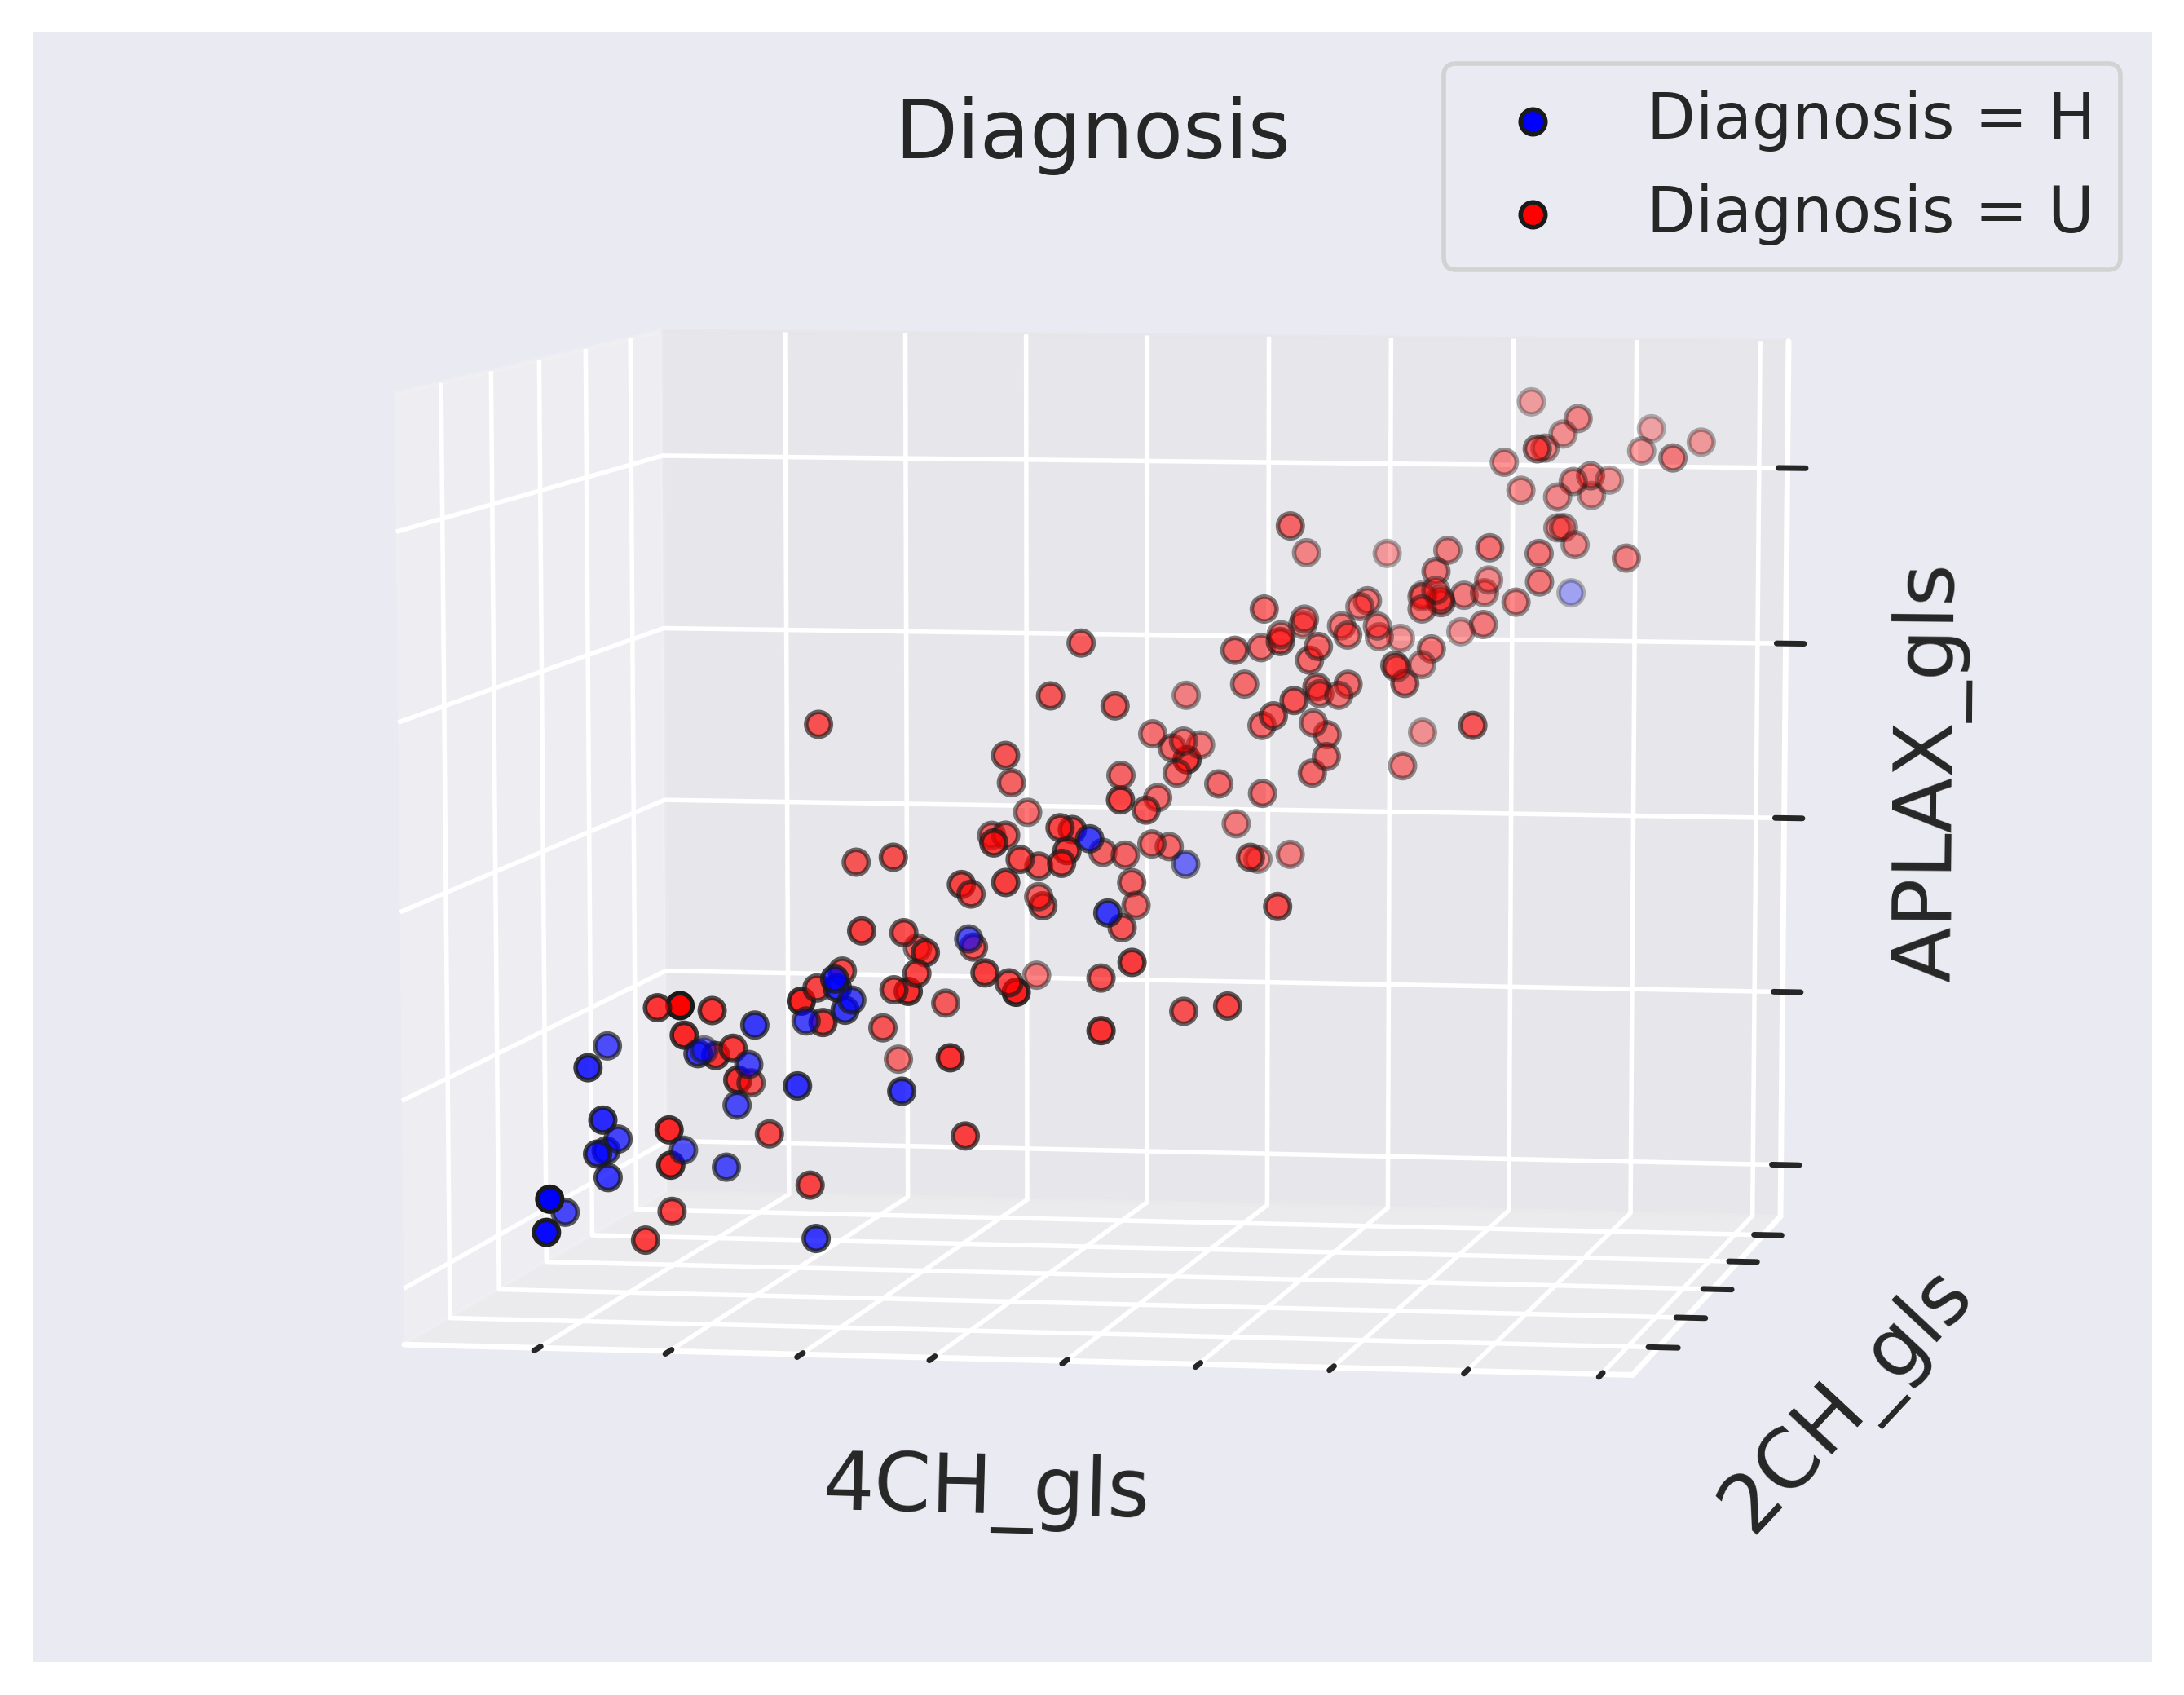
\includegraphics[width=0.99\textwidth]{results/pd/scatter_gls_indication_bin.png}
        \caption{Patient Diagnosis. \textbf{H} stands for \textbf{Healthy}, and \textbf{U} stands for \textbf{Unhealthy}}
        \label{fig:scatter_gls_pd}
    \end{subfigure}
    \begin{subfigure}[b]{0.49\textwidth}
        \centering
        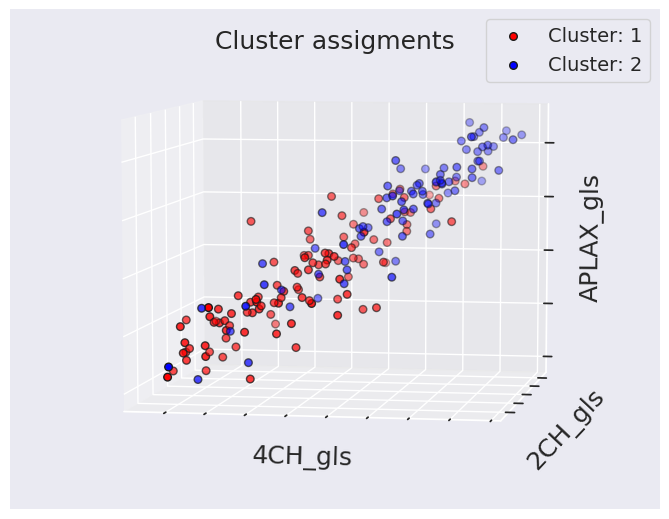
\includegraphics[width=0.99\textwidth]{results/pd/scatter_gls_EF_ward2.png}
        \caption{\textit{GLS-EF Ward/2} cluster assignments.}
        \label{fig:scatter_gls_ef_ward2_ind}
    \end{subfigure}\\
    \begin{subfigure}[b]{0.49\textwidth}
        \centering
        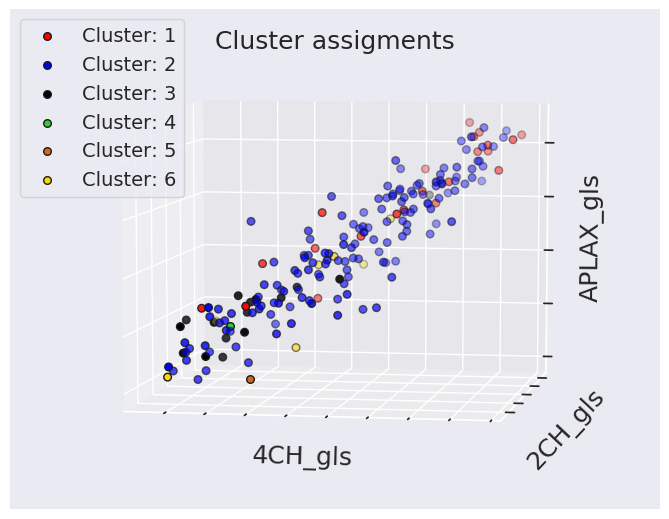
\includegraphics[width=0.99\textwidth]{results/pd/scatter_gls_average6.png}
        \caption{\textit{GLS Average/6} cluster assignments.}
        \label{fig:scatter_gls_average6}
    \end{subfigure}
    \begin{subfigure}[b]{0.49\textwidth}
        \centering
        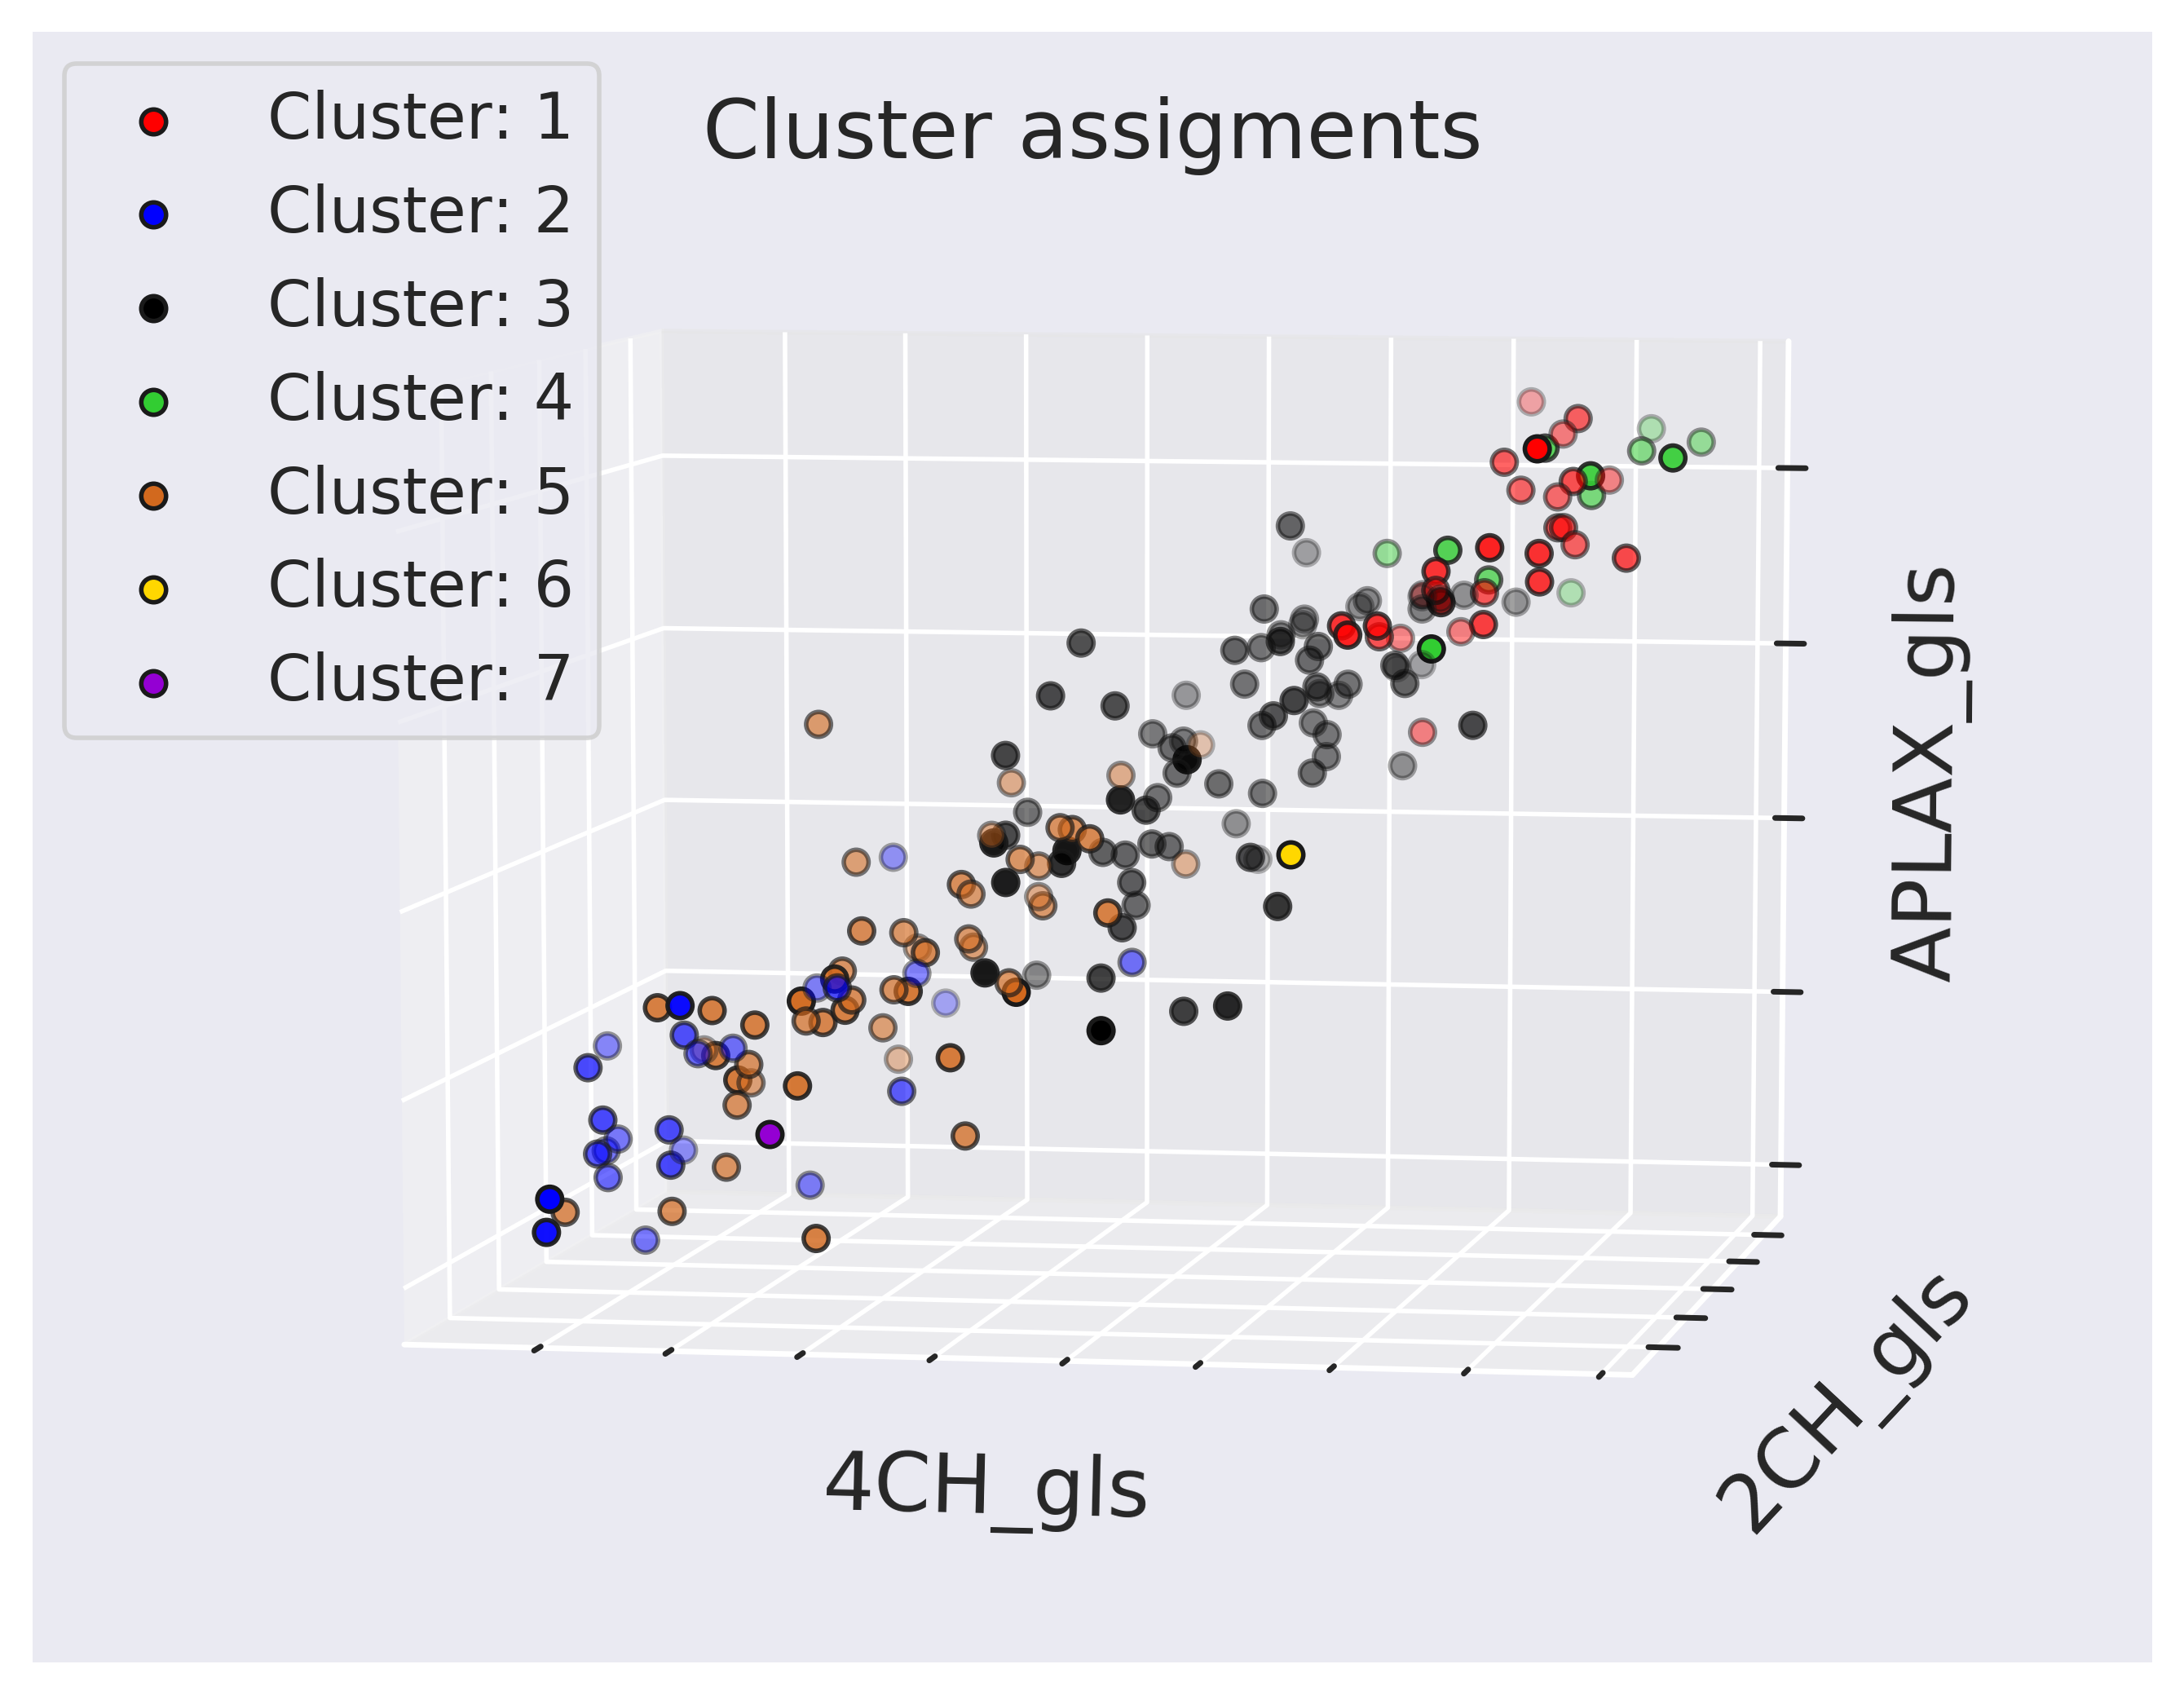
\includegraphics[width=0.99\textwidth]{results/pd/scatter_gls_average7.png}
        \caption{\textit{GLS Average/7} cluster assignments.}
        \label{fig:scatter_gls_average7}
    \end{subfigure}
    \caption{Scatterplot of peak \acrshort{gls} values in each view. Colors in the of the different dots are given by heart failure diagnosis, and cluster assignments of 
             \textit{gls-EF/ward/2}, \textit{average/6} and \textit{average/7} models. Numbers are not included on the axes because the point of the figure is to illustrate the separability 
             of clusters, and patient diagnosis.}
             \label{fig:scatter_gls_ind_cluster_assignments}
\end{figure}

\newpage

\subsection{Artificial Neural Network}

\begin{figure}[H]
    \centering
    %% Creator: Matplotlib, PGF backend
%%
%% To include the figure in your LaTeX document, write
%%   \input{<filename>.pgf}
%%
%% Make sure the required packages are loaded in your preamble
%%   \usepackage{pgf}
%%
%% Figures using additional raster images can only be included by \input if
%% they are in the same directory as the main LaTeX file. For loading figures
%% from other directories you can use the `import` package
%%   \usepackage{import}
%% and then include the figures with
%%   \import{<path to file>}{<filename>.pgf}
%%
%% Matplotlib used the following preamble
%%
\begingroup%
\makeatletter%
\begin{pgfpicture}%
\pgfpathrectangle{\pgfpointorigin}{\pgfqpoint{6.439273in}{2.540000in}}%
\pgfusepath{use as bounding box, clip}%
\begin{pgfscope}%
\pgfsetbuttcap%
\pgfsetmiterjoin%
\definecolor{currentfill}{rgb}{1.000000,1.000000,1.000000}%
\pgfsetfillcolor{currentfill}%
\pgfsetlinewidth{0.000000pt}%
\definecolor{currentstroke}{rgb}{1.000000,1.000000,1.000000}%
\pgfsetstrokecolor{currentstroke}%
\pgfsetdash{}{0pt}%
\pgfpathmoveto{\pgfqpoint{0.000000in}{0.000000in}}%
\pgfpathlineto{\pgfqpoint{6.439273in}{0.000000in}}%
\pgfpathlineto{\pgfqpoint{6.439273in}{2.540000in}}%
\pgfpathlineto{\pgfqpoint{0.000000in}{2.540000in}}%
\pgfpathclose%
\pgfusepath{fill}%
\end{pgfscope}%
\begin{pgfscope}%
\pgfsetbuttcap%
\pgfsetmiterjoin%
\definecolor{currentfill}{rgb}{0.917647,0.917647,0.949020}%
\pgfsetfillcolor{currentfill}%
\pgfsetlinewidth{0.000000pt}%
\definecolor{currentstroke}{rgb}{0.000000,0.000000,0.000000}%
\pgfsetstrokecolor{currentstroke}%
\pgfsetstrokeopacity{0.000000}%
\pgfsetdash{}{0pt}%
\pgfpathmoveto{\pgfqpoint{0.693056in}{0.557870in}}%
\pgfpathlineto{\pgfqpoint{3.156042in}{0.557870in}}%
\pgfpathlineto{\pgfqpoint{3.156042in}{2.242604in}}%
\pgfpathlineto{\pgfqpoint{0.693056in}{2.242604in}}%
\pgfpathclose%
\pgfusepath{fill}%
\end{pgfscope}%
\begin{pgfscope}%
\pgfpathrectangle{\pgfqpoint{0.693056in}{0.557870in}}{\pgfqpoint{2.462986in}{1.684734in}}%
\pgfusepath{clip}%
\pgfsetroundcap%
\pgfsetroundjoin%
\pgfsetlinewidth{1.003750pt}%
\definecolor{currentstroke}{rgb}{1.000000,1.000000,1.000000}%
\pgfsetstrokecolor{currentstroke}%
\pgfsetdash{}{0pt}%
\pgfpathmoveto{\pgfqpoint{0.805010in}{0.557870in}}%
\pgfpathlineto{\pgfqpoint{0.805010in}{2.242604in}}%
\pgfusepath{stroke}%
\end{pgfscope}%
\begin{pgfscope}%
\definecolor{textcolor}{rgb}{0.150000,0.150000,0.150000}%
\pgfsetstrokecolor{textcolor}%
\pgfsetfillcolor{textcolor}%
\pgftext[x=0.805010in,y=0.425926in,,top]{\color{textcolor}\sffamily\fontsize{11.000000}{13.200000}\selectfont \(\displaystyle -0.50\)}%
\end{pgfscope}%
\begin{pgfscope}%
\pgfpathrectangle{\pgfqpoint{0.693056in}{0.557870in}}{\pgfqpoint{2.462986in}{1.684734in}}%
\pgfusepath{clip}%
\pgfsetroundcap%
\pgfsetroundjoin%
\pgfsetlinewidth{1.003750pt}%
\definecolor{currentstroke}{rgb}{1.000000,1.000000,1.000000}%
\pgfsetstrokecolor{currentstroke}%
\pgfsetdash{}{0pt}%
\pgfpathmoveto{\pgfqpoint{1.364779in}{0.557870in}}%
\pgfpathlineto{\pgfqpoint{1.364779in}{2.242604in}}%
\pgfusepath{stroke}%
\end{pgfscope}%
\begin{pgfscope}%
\definecolor{textcolor}{rgb}{0.150000,0.150000,0.150000}%
\pgfsetstrokecolor{textcolor}%
\pgfsetfillcolor{textcolor}%
\pgftext[x=1.364779in,y=0.425926in,,top]{\color{textcolor}\sffamily\fontsize{11.000000}{13.200000}\selectfont \(\displaystyle -0.25\)}%
\end{pgfscope}%
\begin{pgfscope}%
\pgfpathrectangle{\pgfqpoint{0.693056in}{0.557870in}}{\pgfqpoint{2.462986in}{1.684734in}}%
\pgfusepath{clip}%
\pgfsetroundcap%
\pgfsetroundjoin%
\pgfsetlinewidth{1.003750pt}%
\definecolor{currentstroke}{rgb}{1.000000,1.000000,1.000000}%
\pgfsetstrokecolor{currentstroke}%
\pgfsetdash{}{0pt}%
\pgfpathmoveto{\pgfqpoint{1.924549in}{0.557870in}}%
\pgfpathlineto{\pgfqpoint{1.924549in}{2.242604in}}%
\pgfusepath{stroke}%
\end{pgfscope}%
\begin{pgfscope}%
\definecolor{textcolor}{rgb}{0.150000,0.150000,0.150000}%
\pgfsetstrokecolor{textcolor}%
\pgfsetfillcolor{textcolor}%
\pgftext[x=1.924549in,y=0.425926in,,top]{\color{textcolor}\sffamily\fontsize{11.000000}{13.200000}\selectfont \(\displaystyle 0.00\)}%
\end{pgfscope}%
\begin{pgfscope}%
\pgfpathrectangle{\pgfqpoint{0.693056in}{0.557870in}}{\pgfqpoint{2.462986in}{1.684734in}}%
\pgfusepath{clip}%
\pgfsetroundcap%
\pgfsetroundjoin%
\pgfsetlinewidth{1.003750pt}%
\definecolor{currentstroke}{rgb}{1.000000,1.000000,1.000000}%
\pgfsetstrokecolor{currentstroke}%
\pgfsetdash{}{0pt}%
\pgfpathmoveto{\pgfqpoint{2.484318in}{0.557870in}}%
\pgfpathlineto{\pgfqpoint{2.484318in}{2.242604in}}%
\pgfusepath{stroke}%
\end{pgfscope}%
\begin{pgfscope}%
\definecolor{textcolor}{rgb}{0.150000,0.150000,0.150000}%
\pgfsetstrokecolor{textcolor}%
\pgfsetfillcolor{textcolor}%
\pgftext[x=2.484318in,y=0.425926in,,top]{\color{textcolor}\sffamily\fontsize{11.000000}{13.200000}\selectfont \(\displaystyle 0.25\)}%
\end{pgfscope}%
\begin{pgfscope}%
\pgfpathrectangle{\pgfqpoint{0.693056in}{0.557870in}}{\pgfqpoint{2.462986in}{1.684734in}}%
\pgfusepath{clip}%
\pgfsetroundcap%
\pgfsetroundjoin%
\pgfsetlinewidth{1.003750pt}%
\definecolor{currentstroke}{rgb}{1.000000,1.000000,1.000000}%
\pgfsetstrokecolor{currentstroke}%
\pgfsetdash{}{0pt}%
\pgfpathmoveto{\pgfqpoint{3.044088in}{0.557870in}}%
\pgfpathlineto{\pgfqpoint{3.044088in}{2.242604in}}%
\pgfusepath{stroke}%
\end{pgfscope}%
\begin{pgfscope}%
\definecolor{textcolor}{rgb}{0.150000,0.150000,0.150000}%
\pgfsetstrokecolor{textcolor}%
\pgfsetfillcolor{textcolor}%
\pgftext[x=3.044088in,y=0.425926in,,top]{\color{textcolor}\sffamily\fontsize{11.000000}{13.200000}\selectfont \(\displaystyle 0.50\)}%
\end{pgfscope}%
\begin{pgfscope}%
\definecolor{textcolor}{rgb}{0.150000,0.150000,0.150000}%
\pgfsetstrokecolor{textcolor}%
\pgfsetfillcolor{textcolor}%
\pgftext[x=1.924549in,y=0.235185in,,top]{\color{textcolor}\sffamily\fontsize{11.000000}{13.200000}\selectfont DOR}%
\end{pgfscope}%
\begin{pgfscope}%
\pgfpathrectangle{\pgfqpoint{0.693056in}{0.557870in}}{\pgfqpoint{2.462986in}{1.684734in}}%
\pgfusepath{clip}%
\pgfsetroundcap%
\pgfsetroundjoin%
\pgfsetlinewidth{1.003750pt}%
\definecolor{currentstroke}{rgb}{1.000000,1.000000,1.000000}%
\pgfsetstrokecolor{currentstroke}%
\pgfsetdash{}{0pt}%
\pgfpathmoveto{\pgfqpoint{0.693056in}{0.557870in}}%
\pgfpathlineto{\pgfqpoint{3.156042in}{0.557870in}}%
\pgfusepath{stroke}%
\end{pgfscope}%
\begin{pgfscope}%
\definecolor{textcolor}{rgb}{0.150000,0.150000,0.150000}%
\pgfsetstrokecolor{textcolor}%
\pgfsetfillcolor{textcolor}%
\pgftext[x=0.290741in,y=0.505064in,left,base]{\color{textcolor}\sffamily\fontsize{11.000000}{13.200000}\selectfont \(\displaystyle 0.00\)}%
\end{pgfscope}%
\begin{pgfscope}%
\pgfpathrectangle{\pgfqpoint{0.693056in}{0.557870in}}{\pgfqpoint{2.462986in}{1.684734in}}%
\pgfusepath{clip}%
\pgfsetroundcap%
\pgfsetroundjoin%
\pgfsetlinewidth{1.003750pt}%
\definecolor{currentstroke}{rgb}{1.000000,1.000000,1.000000}%
\pgfsetstrokecolor{currentstroke}%
\pgfsetdash{}{0pt}%
\pgfpathmoveto{\pgfqpoint{0.693056in}{0.958997in}}%
\pgfpathlineto{\pgfqpoint{3.156042in}{0.958997in}}%
\pgfusepath{stroke}%
\end{pgfscope}%
\begin{pgfscope}%
\definecolor{textcolor}{rgb}{0.150000,0.150000,0.150000}%
\pgfsetstrokecolor{textcolor}%
\pgfsetfillcolor{textcolor}%
\pgftext[x=0.290741in,y=0.906191in,left,base]{\color{textcolor}\sffamily\fontsize{11.000000}{13.200000}\selectfont \(\displaystyle 0.25\)}%
\end{pgfscope}%
\begin{pgfscope}%
\pgfpathrectangle{\pgfqpoint{0.693056in}{0.557870in}}{\pgfqpoint{2.462986in}{1.684734in}}%
\pgfusepath{clip}%
\pgfsetroundcap%
\pgfsetroundjoin%
\pgfsetlinewidth{1.003750pt}%
\definecolor{currentstroke}{rgb}{1.000000,1.000000,1.000000}%
\pgfsetstrokecolor{currentstroke}%
\pgfsetdash{}{0pt}%
\pgfpathmoveto{\pgfqpoint{0.693056in}{1.360125in}}%
\pgfpathlineto{\pgfqpoint{3.156042in}{1.360125in}}%
\pgfusepath{stroke}%
\end{pgfscope}%
\begin{pgfscope}%
\definecolor{textcolor}{rgb}{0.150000,0.150000,0.150000}%
\pgfsetstrokecolor{textcolor}%
\pgfsetfillcolor{textcolor}%
\pgftext[x=0.290741in,y=1.307318in,left,base]{\color{textcolor}\sffamily\fontsize{11.000000}{13.200000}\selectfont \(\displaystyle 0.50\)}%
\end{pgfscope}%
\begin{pgfscope}%
\pgfpathrectangle{\pgfqpoint{0.693056in}{0.557870in}}{\pgfqpoint{2.462986in}{1.684734in}}%
\pgfusepath{clip}%
\pgfsetroundcap%
\pgfsetroundjoin%
\pgfsetlinewidth{1.003750pt}%
\definecolor{currentstroke}{rgb}{1.000000,1.000000,1.000000}%
\pgfsetstrokecolor{currentstroke}%
\pgfsetdash{}{0pt}%
\pgfpathmoveto{\pgfqpoint{0.693056in}{1.761252in}}%
\pgfpathlineto{\pgfqpoint{3.156042in}{1.761252in}}%
\pgfusepath{stroke}%
\end{pgfscope}%
\begin{pgfscope}%
\definecolor{textcolor}{rgb}{0.150000,0.150000,0.150000}%
\pgfsetstrokecolor{textcolor}%
\pgfsetfillcolor{textcolor}%
\pgftext[x=0.290741in,y=1.708445in,left,base]{\color{textcolor}\sffamily\fontsize{11.000000}{13.200000}\selectfont \(\displaystyle 0.75\)}%
\end{pgfscope}%
\begin{pgfscope}%
\pgfpathrectangle{\pgfqpoint{0.693056in}{0.557870in}}{\pgfqpoint{2.462986in}{1.684734in}}%
\pgfusepath{clip}%
\pgfsetroundcap%
\pgfsetroundjoin%
\pgfsetlinewidth{1.003750pt}%
\definecolor{currentstroke}{rgb}{1.000000,1.000000,1.000000}%
\pgfsetstrokecolor{currentstroke}%
\pgfsetdash{}{0pt}%
\pgfpathmoveto{\pgfqpoint{0.693056in}{2.162379in}}%
\pgfpathlineto{\pgfqpoint{3.156042in}{2.162379in}}%
\pgfusepath{stroke}%
\end{pgfscope}%
\begin{pgfscope}%
\definecolor{textcolor}{rgb}{0.150000,0.150000,0.150000}%
\pgfsetstrokecolor{textcolor}%
\pgfsetfillcolor{textcolor}%
\pgftext[x=0.290741in,y=2.109572in,left,base]{\color{textcolor}\sffamily\fontsize{11.000000}{13.200000}\selectfont \(\displaystyle 1.00\)}%
\end{pgfscope}%
\begin{pgfscope}%
\definecolor{textcolor}{rgb}{0.150000,0.150000,0.150000}%
\pgfsetstrokecolor{textcolor}%
\pgfsetfillcolor{textcolor}%
\pgftext[x=0.235185in,y=1.400237in,,bottom,rotate=90.000000]{\color{textcolor}\sffamily\fontsize{11.000000}{13.200000}\selectfont Occurance}%
\end{pgfscope}%
\begin{pgfscope}%
\pgfpathrectangle{\pgfqpoint{0.693056in}{0.557870in}}{\pgfqpoint{2.462986in}{1.684734in}}%
\pgfusepath{clip}%
\pgfsetbuttcap%
\pgfsetmiterjoin%
\definecolor{currentfill}{rgb}{0.298039,0.447059,0.690196}%
\pgfsetfillcolor{currentfill}%
\pgfsetfillopacity{0.400000}%
\pgfsetlinewidth{1.003750pt}%
\definecolor{currentstroke}{rgb}{1.000000,1.000000,1.000000}%
\pgfsetstrokecolor{currentstroke}%
\pgfsetstrokeopacity{0.400000}%
\pgfsetdash{}{0pt}%
\pgfpathmoveto{\pgfqpoint{0.805010in}{0.557870in}}%
\pgfpathlineto{\pgfqpoint{1.028918in}{0.557870in}}%
\pgfpathlineto{\pgfqpoint{1.028918in}{0.557870in}}%
\pgfpathlineto{\pgfqpoint{0.805010in}{0.557870in}}%
\pgfpathclose%
\pgfusepath{stroke,fill}%
\end{pgfscope}%
\begin{pgfscope}%
\pgfpathrectangle{\pgfqpoint{0.693056in}{0.557870in}}{\pgfqpoint{2.462986in}{1.684734in}}%
\pgfusepath{clip}%
\pgfsetbuttcap%
\pgfsetmiterjoin%
\definecolor{currentfill}{rgb}{0.298039,0.447059,0.690196}%
\pgfsetfillcolor{currentfill}%
\pgfsetfillopacity{0.400000}%
\pgfsetlinewidth{1.003750pt}%
\definecolor{currentstroke}{rgb}{1.000000,1.000000,1.000000}%
\pgfsetstrokecolor{currentstroke}%
\pgfsetstrokeopacity{0.400000}%
\pgfsetdash{}{0pt}%
\pgfpathmoveto{\pgfqpoint{1.028918in}{0.557870in}}%
\pgfpathlineto{\pgfqpoint{1.252825in}{0.557870in}}%
\pgfpathlineto{\pgfqpoint{1.252825in}{0.557870in}}%
\pgfpathlineto{\pgfqpoint{1.028918in}{0.557870in}}%
\pgfpathclose%
\pgfusepath{stroke,fill}%
\end{pgfscope}%
\begin{pgfscope}%
\pgfpathrectangle{\pgfqpoint{0.693056in}{0.557870in}}{\pgfqpoint{2.462986in}{1.684734in}}%
\pgfusepath{clip}%
\pgfsetbuttcap%
\pgfsetmiterjoin%
\definecolor{currentfill}{rgb}{0.298039,0.447059,0.690196}%
\pgfsetfillcolor{currentfill}%
\pgfsetfillopacity{0.400000}%
\pgfsetlinewidth{1.003750pt}%
\definecolor{currentstroke}{rgb}{1.000000,1.000000,1.000000}%
\pgfsetstrokecolor{currentstroke}%
\pgfsetstrokeopacity{0.400000}%
\pgfsetdash{}{0pt}%
\pgfpathmoveto{\pgfqpoint{1.252825in}{0.557870in}}%
\pgfpathlineto{\pgfqpoint{1.476733in}{0.557870in}}%
\pgfpathlineto{\pgfqpoint{1.476733in}{0.557870in}}%
\pgfpathlineto{\pgfqpoint{1.252825in}{0.557870in}}%
\pgfpathclose%
\pgfusepath{stroke,fill}%
\end{pgfscope}%
\begin{pgfscope}%
\pgfpathrectangle{\pgfqpoint{0.693056in}{0.557870in}}{\pgfqpoint{2.462986in}{1.684734in}}%
\pgfusepath{clip}%
\pgfsetbuttcap%
\pgfsetmiterjoin%
\definecolor{currentfill}{rgb}{0.298039,0.447059,0.690196}%
\pgfsetfillcolor{currentfill}%
\pgfsetfillopacity{0.400000}%
\pgfsetlinewidth{1.003750pt}%
\definecolor{currentstroke}{rgb}{1.000000,1.000000,1.000000}%
\pgfsetstrokecolor{currentstroke}%
\pgfsetstrokeopacity{0.400000}%
\pgfsetdash{}{0pt}%
\pgfpathmoveto{\pgfqpoint{1.476733in}{0.557870in}}%
\pgfpathlineto{\pgfqpoint{1.700641in}{0.557870in}}%
\pgfpathlineto{\pgfqpoint{1.700641in}{0.557870in}}%
\pgfpathlineto{\pgfqpoint{1.476733in}{0.557870in}}%
\pgfpathclose%
\pgfusepath{stroke,fill}%
\end{pgfscope}%
\begin{pgfscope}%
\pgfpathrectangle{\pgfqpoint{0.693056in}{0.557870in}}{\pgfqpoint{2.462986in}{1.684734in}}%
\pgfusepath{clip}%
\pgfsetbuttcap%
\pgfsetmiterjoin%
\definecolor{currentfill}{rgb}{0.298039,0.447059,0.690196}%
\pgfsetfillcolor{currentfill}%
\pgfsetfillopacity{0.400000}%
\pgfsetlinewidth{1.003750pt}%
\definecolor{currentstroke}{rgb}{1.000000,1.000000,1.000000}%
\pgfsetstrokecolor{currentstroke}%
\pgfsetstrokeopacity{0.400000}%
\pgfsetdash{}{0pt}%
\pgfpathmoveto{\pgfqpoint{1.700641in}{0.557870in}}%
\pgfpathlineto{\pgfqpoint{1.924549in}{0.557870in}}%
\pgfpathlineto{\pgfqpoint{1.924549in}{0.557870in}}%
\pgfpathlineto{\pgfqpoint{1.700641in}{0.557870in}}%
\pgfpathclose%
\pgfusepath{stroke,fill}%
\end{pgfscope}%
\begin{pgfscope}%
\pgfpathrectangle{\pgfqpoint{0.693056in}{0.557870in}}{\pgfqpoint{2.462986in}{1.684734in}}%
\pgfusepath{clip}%
\pgfsetbuttcap%
\pgfsetmiterjoin%
\definecolor{currentfill}{rgb}{0.298039,0.447059,0.690196}%
\pgfsetfillcolor{currentfill}%
\pgfsetfillopacity{0.400000}%
\pgfsetlinewidth{1.003750pt}%
\definecolor{currentstroke}{rgb}{1.000000,1.000000,1.000000}%
\pgfsetstrokecolor{currentstroke}%
\pgfsetstrokeopacity{0.400000}%
\pgfsetdash{}{0pt}%
\pgfpathmoveto{\pgfqpoint{1.924549in}{0.557870in}}%
\pgfpathlineto{\pgfqpoint{2.148457in}{0.557870in}}%
\pgfpathlineto{\pgfqpoint{2.148457in}{2.162379in}}%
\pgfpathlineto{\pgfqpoint{1.924549in}{2.162379in}}%
\pgfpathclose%
\pgfusepath{stroke,fill}%
\end{pgfscope}%
\begin{pgfscope}%
\pgfpathrectangle{\pgfqpoint{0.693056in}{0.557870in}}{\pgfqpoint{2.462986in}{1.684734in}}%
\pgfusepath{clip}%
\pgfsetbuttcap%
\pgfsetmiterjoin%
\definecolor{currentfill}{rgb}{0.298039,0.447059,0.690196}%
\pgfsetfillcolor{currentfill}%
\pgfsetfillopacity{0.400000}%
\pgfsetlinewidth{1.003750pt}%
\definecolor{currentstroke}{rgb}{1.000000,1.000000,1.000000}%
\pgfsetstrokecolor{currentstroke}%
\pgfsetstrokeopacity{0.400000}%
\pgfsetdash{}{0pt}%
\pgfpathmoveto{\pgfqpoint{2.148457in}{0.557870in}}%
\pgfpathlineto{\pgfqpoint{2.372364in}{0.557870in}}%
\pgfpathlineto{\pgfqpoint{2.372364in}{0.557870in}}%
\pgfpathlineto{\pgfqpoint{2.148457in}{0.557870in}}%
\pgfpathclose%
\pgfusepath{stroke,fill}%
\end{pgfscope}%
\begin{pgfscope}%
\pgfpathrectangle{\pgfqpoint{0.693056in}{0.557870in}}{\pgfqpoint{2.462986in}{1.684734in}}%
\pgfusepath{clip}%
\pgfsetbuttcap%
\pgfsetmiterjoin%
\definecolor{currentfill}{rgb}{0.298039,0.447059,0.690196}%
\pgfsetfillcolor{currentfill}%
\pgfsetfillopacity{0.400000}%
\pgfsetlinewidth{1.003750pt}%
\definecolor{currentstroke}{rgb}{1.000000,1.000000,1.000000}%
\pgfsetstrokecolor{currentstroke}%
\pgfsetstrokeopacity{0.400000}%
\pgfsetdash{}{0pt}%
\pgfpathmoveto{\pgfqpoint{2.372364in}{0.557870in}}%
\pgfpathlineto{\pgfqpoint{2.596272in}{0.557870in}}%
\pgfpathlineto{\pgfqpoint{2.596272in}{0.557870in}}%
\pgfpathlineto{\pgfqpoint{2.372364in}{0.557870in}}%
\pgfpathclose%
\pgfusepath{stroke,fill}%
\end{pgfscope}%
\begin{pgfscope}%
\pgfpathrectangle{\pgfqpoint{0.693056in}{0.557870in}}{\pgfqpoint{2.462986in}{1.684734in}}%
\pgfusepath{clip}%
\pgfsetbuttcap%
\pgfsetmiterjoin%
\definecolor{currentfill}{rgb}{0.298039,0.447059,0.690196}%
\pgfsetfillcolor{currentfill}%
\pgfsetfillopacity{0.400000}%
\pgfsetlinewidth{1.003750pt}%
\definecolor{currentstroke}{rgb}{1.000000,1.000000,1.000000}%
\pgfsetstrokecolor{currentstroke}%
\pgfsetstrokeopacity{0.400000}%
\pgfsetdash{}{0pt}%
\pgfpathmoveto{\pgfqpoint{2.596272in}{0.557870in}}%
\pgfpathlineto{\pgfqpoint{2.820180in}{0.557870in}}%
\pgfpathlineto{\pgfqpoint{2.820180in}{0.557870in}}%
\pgfpathlineto{\pgfqpoint{2.596272in}{0.557870in}}%
\pgfpathclose%
\pgfusepath{stroke,fill}%
\end{pgfscope}%
\begin{pgfscope}%
\pgfpathrectangle{\pgfqpoint{0.693056in}{0.557870in}}{\pgfqpoint{2.462986in}{1.684734in}}%
\pgfusepath{clip}%
\pgfsetbuttcap%
\pgfsetmiterjoin%
\definecolor{currentfill}{rgb}{0.298039,0.447059,0.690196}%
\pgfsetfillcolor{currentfill}%
\pgfsetfillopacity{0.400000}%
\pgfsetlinewidth{1.003750pt}%
\definecolor{currentstroke}{rgb}{1.000000,1.000000,1.000000}%
\pgfsetstrokecolor{currentstroke}%
\pgfsetstrokeopacity{0.400000}%
\pgfsetdash{}{0pt}%
\pgfpathmoveto{\pgfqpoint{2.820180in}{0.557870in}}%
\pgfpathlineto{\pgfqpoint{3.044088in}{0.557870in}}%
\pgfpathlineto{\pgfqpoint{3.044088in}{0.557870in}}%
\pgfpathlineto{\pgfqpoint{2.820180in}{0.557870in}}%
\pgfpathclose%
\pgfusepath{stroke,fill}%
\end{pgfscope}%
\begin{pgfscope}%
\pgfsetrectcap%
\pgfsetmiterjoin%
\pgfsetlinewidth{1.254687pt}%
\definecolor{currentstroke}{rgb}{1.000000,1.000000,1.000000}%
\pgfsetstrokecolor{currentstroke}%
\pgfsetdash{}{0pt}%
\pgfpathmoveto{\pgfqpoint{0.693056in}{0.557870in}}%
\pgfpathlineto{\pgfqpoint{0.693056in}{2.242604in}}%
\pgfusepath{stroke}%
\end{pgfscope}%
\begin{pgfscope}%
\pgfsetrectcap%
\pgfsetmiterjoin%
\pgfsetlinewidth{1.254687pt}%
\definecolor{currentstroke}{rgb}{1.000000,1.000000,1.000000}%
\pgfsetstrokecolor{currentstroke}%
\pgfsetdash{}{0pt}%
\pgfpathmoveto{\pgfqpoint{3.156042in}{0.557870in}}%
\pgfpathlineto{\pgfqpoint{3.156042in}{2.242604in}}%
\pgfusepath{stroke}%
\end{pgfscope}%
\begin{pgfscope}%
\pgfsetrectcap%
\pgfsetmiterjoin%
\pgfsetlinewidth{1.254687pt}%
\definecolor{currentstroke}{rgb}{1.000000,1.000000,1.000000}%
\pgfsetstrokecolor{currentstroke}%
\pgfsetdash{}{0pt}%
\pgfpathmoveto{\pgfqpoint{0.693056in}{0.557870in}}%
\pgfpathlineto{\pgfqpoint{3.156042in}{0.557870in}}%
\pgfusepath{stroke}%
\end{pgfscope}%
\begin{pgfscope}%
\pgfsetrectcap%
\pgfsetmiterjoin%
\pgfsetlinewidth{1.254687pt}%
\definecolor{currentstroke}{rgb}{1.000000,1.000000,1.000000}%
\pgfsetstrokecolor{currentstroke}%
\pgfsetdash{}{0pt}%
\pgfpathmoveto{\pgfqpoint{0.693056in}{2.242604in}}%
\pgfpathlineto{\pgfqpoint{3.156042in}{2.242604in}}%
\pgfusepath{stroke}%
\end{pgfscope}%
\begin{pgfscope}%
\definecolor{textcolor}{rgb}{0.150000,0.150000,0.150000}%
\pgfsetstrokecolor{textcolor}%
\pgfsetfillcolor{textcolor}%
\pgftext[x=1.924549in,y=2.325938in,,base]{\color{textcolor}\sffamily\fontsize{11.000000}{13.200000}\selectfont (a)}%
\end{pgfscope}%
\begin{pgfscope}%
\pgfsetbuttcap%
\pgfsetmiterjoin%
\definecolor{currentfill}{rgb}{0.917647,0.917647,0.949020}%
\pgfsetfillcolor{currentfill}%
\pgfsetlinewidth{0.000000pt}%
\definecolor{currentstroke}{rgb}{0.000000,0.000000,0.000000}%
\pgfsetstrokecolor{currentstroke}%
\pgfsetstrokeopacity{0.000000}%
\pgfsetdash{}{0pt}%
\pgfpathmoveto{\pgfqpoint{3.853056in}{0.557870in}}%
\pgfpathlineto{\pgfqpoint{6.316042in}{0.557870in}}%
\pgfpathlineto{\pgfqpoint{6.316042in}{2.242604in}}%
\pgfpathlineto{\pgfqpoint{3.853056in}{2.242604in}}%
\pgfpathclose%
\pgfusepath{fill}%
\end{pgfscope}%
\begin{pgfscope}%
\pgfpathrectangle{\pgfqpoint{3.853056in}{0.557870in}}{\pgfqpoint{2.462986in}{1.684734in}}%
\pgfusepath{clip}%
\pgfsetroundcap%
\pgfsetroundjoin%
\pgfsetlinewidth{1.003750pt}%
\definecolor{currentstroke}{rgb}{1.000000,1.000000,1.000000}%
\pgfsetstrokecolor{currentstroke}%
\pgfsetdash{}{0pt}%
\pgfpathmoveto{\pgfqpoint{3.965010in}{0.557870in}}%
\pgfpathlineto{\pgfqpoint{3.965010in}{2.242604in}}%
\pgfusepath{stroke}%
\end{pgfscope}%
\begin{pgfscope}%
\definecolor{textcolor}{rgb}{0.150000,0.150000,0.150000}%
\pgfsetstrokecolor{textcolor}%
\pgfsetfillcolor{textcolor}%
\pgftext[x=3.965010in,y=0.425926in,,top]{\color{textcolor}\sffamily\fontsize{11.000000}{13.200000}\selectfont \(\displaystyle 0.00\)}%
\end{pgfscope}%
\begin{pgfscope}%
\pgfpathrectangle{\pgfqpoint{3.853056in}{0.557870in}}{\pgfqpoint{2.462986in}{1.684734in}}%
\pgfusepath{clip}%
\pgfsetroundcap%
\pgfsetroundjoin%
\pgfsetlinewidth{1.003750pt}%
\definecolor{currentstroke}{rgb}{1.000000,1.000000,1.000000}%
\pgfsetstrokecolor{currentstroke}%
\pgfsetdash{}{0pt}%
\pgfpathmoveto{\pgfqpoint{4.524779in}{0.557870in}}%
\pgfpathlineto{\pgfqpoint{4.524779in}{2.242604in}}%
\pgfusepath{stroke}%
\end{pgfscope}%
\begin{pgfscope}%
\definecolor{textcolor}{rgb}{0.150000,0.150000,0.150000}%
\pgfsetstrokecolor{textcolor}%
\pgfsetfillcolor{textcolor}%
\pgftext[x=4.524779in,y=0.425926in,,top]{\color{textcolor}\sffamily\fontsize{11.000000}{13.200000}\selectfont \(\displaystyle 0.25\)}%
\end{pgfscope}%
\begin{pgfscope}%
\pgfpathrectangle{\pgfqpoint{3.853056in}{0.557870in}}{\pgfqpoint{2.462986in}{1.684734in}}%
\pgfusepath{clip}%
\pgfsetroundcap%
\pgfsetroundjoin%
\pgfsetlinewidth{1.003750pt}%
\definecolor{currentstroke}{rgb}{1.000000,1.000000,1.000000}%
\pgfsetstrokecolor{currentstroke}%
\pgfsetdash{}{0pt}%
\pgfpathmoveto{\pgfqpoint{5.084549in}{0.557870in}}%
\pgfpathlineto{\pgfqpoint{5.084549in}{2.242604in}}%
\pgfusepath{stroke}%
\end{pgfscope}%
\begin{pgfscope}%
\definecolor{textcolor}{rgb}{0.150000,0.150000,0.150000}%
\pgfsetstrokecolor{textcolor}%
\pgfsetfillcolor{textcolor}%
\pgftext[x=5.084549in,y=0.425926in,,top]{\color{textcolor}\sffamily\fontsize{11.000000}{13.200000}\selectfont \(\displaystyle 0.50\)}%
\end{pgfscope}%
\begin{pgfscope}%
\pgfpathrectangle{\pgfqpoint{3.853056in}{0.557870in}}{\pgfqpoint{2.462986in}{1.684734in}}%
\pgfusepath{clip}%
\pgfsetroundcap%
\pgfsetroundjoin%
\pgfsetlinewidth{1.003750pt}%
\definecolor{currentstroke}{rgb}{1.000000,1.000000,1.000000}%
\pgfsetstrokecolor{currentstroke}%
\pgfsetdash{}{0pt}%
\pgfpathmoveto{\pgfqpoint{5.644318in}{0.557870in}}%
\pgfpathlineto{\pgfqpoint{5.644318in}{2.242604in}}%
\pgfusepath{stroke}%
\end{pgfscope}%
\begin{pgfscope}%
\definecolor{textcolor}{rgb}{0.150000,0.150000,0.150000}%
\pgfsetstrokecolor{textcolor}%
\pgfsetfillcolor{textcolor}%
\pgftext[x=5.644318in,y=0.425926in,,top]{\color{textcolor}\sffamily\fontsize{11.000000}{13.200000}\selectfont \(\displaystyle 0.75\)}%
\end{pgfscope}%
\begin{pgfscope}%
\pgfpathrectangle{\pgfqpoint{3.853056in}{0.557870in}}{\pgfqpoint{2.462986in}{1.684734in}}%
\pgfusepath{clip}%
\pgfsetroundcap%
\pgfsetroundjoin%
\pgfsetlinewidth{1.003750pt}%
\definecolor{currentstroke}{rgb}{1.000000,1.000000,1.000000}%
\pgfsetstrokecolor{currentstroke}%
\pgfsetdash{}{0pt}%
\pgfpathmoveto{\pgfqpoint{6.204088in}{0.557870in}}%
\pgfpathlineto{\pgfqpoint{6.204088in}{2.242604in}}%
\pgfusepath{stroke}%
\end{pgfscope}%
\begin{pgfscope}%
\definecolor{textcolor}{rgb}{0.150000,0.150000,0.150000}%
\pgfsetstrokecolor{textcolor}%
\pgfsetfillcolor{textcolor}%
\pgftext[x=6.204088in,y=0.425926in,,top]{\color{textcolor}\sffamily\fontsize{11.000000}{13.200000}\selectfont \(\displaystyle 1.00\)}%
\end{pgfscope}%
\begin{pgfscope}%
\definecolor{textcolor}{rgb}{0.150000,0.150000,0.150000}%
\pgfsetstrokecolor{textcolor}%
\pgfsetfillcolor{textcolor}%
\pgftext[x=5.084549in,y=0.235185in,,top]{\color{textcolor}\sffamily\fontsize{11.000000}{13.200000}\selectfont Specificity}%
\end{pgfscope}%
\begin{pgfscope}%
\pgfpathrectangle{\pgfqpoint{3.853056in}{0.557870in}}{\pgfqpoint{2.462986in}{1.684734in}}%
\pgfusepath{clip}%
\pgfsetroundcap%
\pgfsetroundjoin%
\pgfsetlinewidth{1.003750pt}%
\definecolor{currentstroke}{rgb}{1.000000,1.000000,1.000000}%
\pgfsetstrokecolor{currentstroke}%
\pgfsetdash{}{0pt}%
\pgfpathmoveto{\pgfqpoint{3.853056in}{0.634449in}}%
\pgfpathlineto{\pgfqpoint{6.316042in}{0.634449in}}%
\pgfusepath{stroke}%
\end{pgfscope}%
\begin{pgfscope}%
\definecolor{textcolor}{rgb}{0.150000,0.150000,0.150000}%
\pgfsetstrokecolor{textcolor}%
\pgfsetfillcolor{textcolor}%
\pgftext[x=3.450741in,y=0.581642in,left,base]{\color{textcolor}\sffamily\fontsize{11.000000}{13.200000}\selectfont \(\displaystyle 0.00\)}%
\end{pgfscope}%
\begin{pgfscope}%
\pgfpathrectangle{\pgfqpoint{3.853056in}{0.557870in}}{\pgfqpoint{2.462986in}{1.684734in}}%
\pgfusepath{clip}%
\pgfsetroundcap%
\pgfsetroundjoin%
\pgfsetlinewidth{1.003750pt}%
\definecolor{currentstroke}{rgb}{1.000000,1.000000,1.000000}%
\pgfsetstrokecolor{currentstroke}%
\pgfsetdash{}{0pt}%
\pgfpathmoveto{\pgfqpoint{3.853056in}{1.017343in}}%
\pgfpathlineto{\pgfqpoint{6.316042in}{1.017343in}}%
\pgfusepath{stroke}%
\end{pgfscope}%
\begin{pgfscope}%
\definecolor{textcolor}{rgb}{0.150000,0.150000,0.150000}%
\pgfsetstrokecolor{textcolor}%
\pgfsetfillcolor{textcolor}%
\pgftext[x=3.450741in,y=0.964536in,left,base]{\color{textcolor}\sffamily\fontsize{11.000000}{13.200000}\selectfont \(\displaystyle 0.25\)}%
\end{pgfscope}%
\begin{pgfscope}%
\pgfpathrectangle{\pgfqpoint{3.853056in}{0.557870in}}{\pgfqpoint{2.462986in}{1.684734in}}%
\pgfusepath{clip}%
\pgfsetroundcap%
\pgfsetroundjoin%
\pgfsetlinewidth{1.003750pt}%
\definecolor{currentstroke}{rgb}{1.000000,1.000000,1.000000}%
\pgfsetstrokecolor{currentstroke}%
\pgfsetdash{}{0pt}%
\pgfpathmoveto{\pgfqpoint{3.853056in}{1.400237in}}%
\pgfpathlineto{\pgfqpoint{6.316042in}{1.400237in}}%
\pgfusepath{stroke}%
\end{pgfscope}%
\begin{pgfscope}%
\definecolor{textcolor}{rgb}{0.150000,0.150000,0.150000}%
\pgfsetstrokecolor{textcolor}%
\pgfsetfillcolor{textcolor}%
\pgftext[x=3.450741in,y=1.347431in,left,base]{\color{textcolor}\sffamily\fontsize{11.000000}{13.200000}\selectfont \(\displaystyle 0.50\)}%
\end{pgfscope}%
\begin{pgfscope}%
\pgfpathrectangle{\pgfqpoint{3.853056in}{0.557870in}}{\pgfqpoint{2.462986in}{1.684734in}}%
\pgfusepath{clip}%
\pgfsetroundcap%
\pgfsetroundjoin%
\pgfsetlinewidth{1.003750pt}%
\definecolor{currentstroke}{rgb}{1.000000,1.000000,1.000000}%
\pgfsetstrokecolor{currentstroke}%
\pgfsetdash{}{0pt}%
\pgfpathmoveto{\pgfqpoint{3.853056in}{1.783131in}}%
\pgfpathlineto{\pgfqpoint{6.316042in}{1.783131in}}%
\pgfusepath{stroke}%
\end{pgfscope}%
\begin{pgfscope}%
\definecolor{textcolor}{rgb}{0.150000,0.150000,0.150000}%
\pgfsetstrokecolor{textcolor}%
\pgfsetfillcolor{textcolor}%
\pgftext[x=3.450741in,y=1.730325in,left,base]{\color{textcolor}\sffamily\fontsize{11.000000}{13.200000}\selectfont \(\displaystyle 0.75\)}%
\end{pgfscope}%
\begin{pgfscope}%
\pgfpathrectangle{\pgfqpoint{3.853056in}{0.557870in}}{\pgfqpoint{2.462986in}{1.684734in}}%
\pgfusepath{clip}%
\pgfsetroundcap%
\pgfsetroundjoin%
\pgfsetlinewidth{1.003750pt}%
\definecolor{currentstroke}{rgb}{1.000000,1.000000,1.000000}%
\pgfsetstrokecolor{currentstroke}%
\pgfsetdash{}{0pt}%
\pgfpathmoveto{\pgfqpoint{3.853056in}{2.166025in}}%
\pgfpathlineto{\pgfqpoint{6.316042in}{2.166025in}}%
\pgfusepath{stroke}%
\end{pgfscope}%
\begin{pgfscope}%
\definecolor{textcolor}{rgb}{0.150000,0.150000,0.150000}%
\pgfsetstrokecolor{textcolor}%
\pgfsetfillcolor{textcolor}%
\pgftext[x=3.450741in,y=2.113219in,left,base]{\color{textcolor}\sffamily\fontsize{11.000000}{13.200000}\selectfont \(\displaystyle 1.00\)}%
\end{pgfscope}%
\begin{pgfscope}%
\definecolor{textcolor}{rgb}{0.150000,0.150000,0.150000}%
\pgfsetstrokecolor{textcolor}%
\pgfsetfillcolor{textcolor}%
\pgftext[x=3.395185in,y=1.400237in,,bottom,rotate=90.000000]{\color{textcolor}\sffamily\fontsize{11.000000}{13.200000}\selectfont Sensitivity}%
\end{pgfscope}%
\begin{pgfscope}%
\pgfpathrectangle{\pgfqpoint{3.853056in}{0.557870in}}{\pgfqpoint{2.462986in}{1.684734in}}%
\pgfusepath{clip}%
\pgfsetbuttcap%
\pgfsetroundjoin%
\definecolor{currentfill}{rgb}{0.298039,0.447059,0.690196}%
\pgfsetfillcolor{currentfill}%
\pgfsetlinewidth{1.003750pt}%
\definecolor{currentstroke}{rgb}{0.298039,0.447059,0.690196}%
\pgfsetstrokecolor{currentstroke}%
\pgfsetdash{}{0pt}%
\pgfpathmoveto{\pgfqpoint{3.965010in}{2.125798in}}%
\pgfpathcurveto{\pgfqpoint{3.973246in}{2.125798in}}{\pgfqpoint{3.981146in}{2.129070in}}{\pgfqpoint{3.986970in}{2.134894in}}%
\pgfpathcurveto{\pgfqpoint{3.992794in}{2.140718in}}{\pgfqpoint{3.996066in}{2.148618in}}{\pgfqpoint{3.996066in}{2.156854in}}%
\pgfpathcurveto{\pgfqpoint{3.996066in}{2.165091in}}{\pgfqpoint{3.992794in}{2.172991in}}{\pgfqpoint{3.986970in}{2.178814in}}%
\pgfpathcurveto{\pgfqpoint{3.981146in}{2.184638in}}{\pgfqpoint{3.973246in}{2.187911in}}{\pgfqpoint{3.965010in}{2.187911in}}%
\pgfpathcurveto{\pgfqpoint{3.956773in}{2.187911in}}{\pgfqpoint{3.948873in}{2.184638in}}{\pgfqpoint{3.943049in}{2.178814in}}%
\pgfpathcurveto{\pgfqpoint{3.937226in}{2.172991in}}{\pgfqpoint{3.933953in}{2.165091in}}{\pgfqpoint{3.933953in}{2.156854in}}%
\pgfpathcurveto{\pgfqpoint{3.933953in}{2.148618in}}{\pgfqpoint{3.937226in}{2.140718in}}{\pgfqpoint{3.943049in}{2.134894in}}%
\pgfpathcurveto{\pgfqpoint{3.948873in}{2.129070in}}{\pgfqpoint{3.956773in}{2.125798in}}{\pgfqpoint{3.965010in}{2.125798in}}%
\pgfpathclose%
\pgfusepath{stroke,fill}%
\end{pgfscope}%
\begin{pgfscope}%
\pgfsetrectcap%
\pgfsetmiterjoin%
\pgfsetlinewidth{1.254687pt}%
\definecolor{currentstroke}{rgb}{1.000000,1.000000,1.000000}%
\pgfsetstrokecolor{currentstroke}%
\pgfsetdash{}{0pt}%
\pgfpathmoveto{\pgfqpoint{3.853056in}{0.557870in}}%
\pgfpathlineto{\pgfqpoint{3.853056in}{2.242604in}}%
\pgfusepath{stroke}%
\end{pgfscope}%
\begin{pgfscope}%
\pgfsetrectcap%
\pgfsetmiterjoin%
\pgfsetlinewidth{1.254687pt}%
\definecolor{currentstroke}{rgb}{1.000000,1.000000,1.000000}%
\pgfsetstrokecolor{currentstroke}%
\pgfsetdash{}{0pt}%
\pgfpathmoveto{\pgfqpoint{6.316042in}{0.557870in}}%
\pgfpathlineto{\pgfqpoint{6.316042in}{2.242604in}}%
\pgfusepath{stroke}%
\end{pgfscope}%
\begin{pgfscope}%
\pgfsetrectcap%
\pgfsetmiterjoin%
\pgfsetlinewidth{1.254687pt}%
\definecolor{currentstroke}{rgb}{1.000000,1.000000,1.000000}%
\pgfsetstrokecolor{currentstroke}%
\pgfsetdash{}{0pt}%
\pgfpathmoveto{\pgfqpoint{3.853056in}{0.557870in}}%
\pgfpathlineto{\pgfqpoint{6.316042in}{0.557870in}}%
\pgfusepath{stroke}%
\end{pgfscope}%
\begin{pgfscope}%
\pgfsetrectcap%
\pgfsetmiterjoin%
\pgfsetlinewidth{1.254687pt}%
\definecolor{currentstroke}{rgb}{1.000000,1.000000,1.000000}%
\pgfsetstrokecolor{currentstroke}%
\pgfsetdash{}{0pt}%
\pgfpathmoveto{\pgfqpoint{3.853056in}{2.242604in}}%
\pgfpathlineto{\pgfqpoint{6.316042in}{2.242604in}}%
\pgfusepath{stroke}%
\end{pgfscope}%
\begin{pgfscope}%
\definecolor{textcolor}{rgb}{0.150000,0.150000,0.150000}%
\pgfsetstrokecolor{textcolor}%
\pgfsetfillcolor{textcolor}%
\pgftext[x=5.084549in,y=2.325938in,,base]{\color{textcolor}\sffamily\fontsize{11.000000}{13.200000}\selectfont (b)}%
\end{pgfscope}%
\end{pgfpicture}%
\makeatother%
\endgroup%

    \caption{(a) Distribution plot of \acrshort{dor} of all \acrshort{ann} models when trained to classify patient diagnosis.
             (b) Scatter plot of the same models sensitivity, and specificity.}
    \label{fig:dl_ind_dor_sens_spec_dist}
\end{figure}

\begin{table*}
    \centering
    \ra{1.3}
    \begin{tabular}{lrrrr}
        \toprule
        Dataset-model              &  Accuracy &  Sensitivity &  Specificity &  \acrshort{dor} \\
        \midrule
        all-strain/4CH/upsampled   &      0.83 &         0.99 &         0.00 & 0.00 \\
        all-strain/2CH/regular     &      0.85 &         1.00 &         0.00 &  NaN \\
        gls/2CH/regular            &      0.85 &         1.00 &         0.00 &  NaN \\
        rls/2CH/regular            &      0.85 &         1.00 &         0.00 &  NaN \\
        all-strain/2CH/downsampled &      0.85 &         1.00 &         0.00 &  NaN \\
        \bottomrule
    \end{tabular}
    \caption{The accuracy, \acrshort{dor}, sensitivity and specicity scores of the five best performing variations of the \acrshort{ann} in terms of \acrshort{dor}, when trained to predict patient diagnoses.
             The \textbf{Dataset-model} column indicates \textit{Dataset used}$/$\textit{View used}$/$\textit{Whether curve has been upsampled, downsampled or is regular}.}
    \label{tab:dl_hf_dor_sens_spec_dist}
\end{table*}

From the distribution plot in figure \ref{fig:dl_ind_dor_sens_spec_dist} one can see that the collective performance of the different variations of the \acrshort{ann} trained to predict patient diagnosis is terrible. The \acrshort{dor} of all the models are either zero because the number of \acrshort{tn} attained are zero, or not defined because the number of \acrshort{fn} are zero. The sensitivities are all 1, or close to 1, and the specificities are all 0. It is evident that the \acrshort{ann} are not able to generalize the traits of the healthy patients from such a small dataset. The \acrshort{ann} models are will therefore not be discussed further with relation to prediction of patient diagnosis, and are not included in the comparison of the four model groups.

\newpage

\subsection{Peak-value Classifiers}

\begin{figure}[H]
    \centering
    % \includegraphics[width=\textwidth]{results/pvmlc_ind_dor_sens_spec_dist.png}
    %% Creator: Matplotlib, PGF backend
%%
%% To include the figure in your LaTeX document, write
%%   \input{<filename>.pgf}
%%
%% Make sure the required packages are loaded in your preamble
%%   \usepackage{pgf}
%%
%% Figures using additional raster images can only be included by \input if
%% they are in the same directory as the main LaTeX file. For loading figures
%% from other directories you can use the `import` package
%%   \usepackage{import}
%% and then include the figures with
%%   \import{<path to file>}{<filename>.pgf}
%%
%% Matplotlib used the following preamble
%%
\begingroup%
\makeatletter%
\begin{pgfpicture}%
\pgfpathrectangle{\pgfpointorigin}{\pgfqpoint{6.362271in}{2.540000in}}%
\pgfusepath{use as bounding box, clip}%
\begin{pgfscope}%
\pgfsetbuttcap%
\pgfsetmiterjoin%
\definecolor{currentfill}{rgb}{1.000000,1.000000,1.000000}%
\pgfsetfillcolor{currentfill}%
\pgfsetlinewidth{0.000000pt}%
\definecolor{currentstroke}{rgb}{1.000000,1.000000,1.000000}%
\pgfsetstrokecolor{currentstroke}%
\pgfsetdash{}{0pt}%
\pgfpathmoveto{\pgfqpoint{0.000000in}{0.000000in}}%
\pgfpathlineto{\pgfqpoint{6.362271in}{0.000000in}}%
\pgfpathlineto{\pgfqpoint{6.362271in}{2.540000in}}%
\pgfpathlineto{\pgfqpoint{0.000000in}{2.540000in}}%
\pgfpathclose%
\pgfusepath{fill}%
\end{pgfscope}%
\begin{pgfscope}%
\pgfsetbuttcap%
\pgfsetmiterjoin%
\definecolor{currentfill}{rgb}{0.917647,0.917647,0.949020}%
\pgfsetfillcolor{currentfill}%
\pgfsetlinewidth{0.000000pt}%
\definecolor{currentstroke}{rgb}{0.000000,0.000000,0.000000}%
\pgfsetstrokecolor{currentstroke}%
\pgfsetstrokeopacity{0.000000}%
\pgfsetdash{}{0pt}%
\pgfpathmoveto{\pgfqpoint{0.574769in}{0.557870in}}%
\pgfpathlineto{\pgfqpoint{3.058877in}{0.557870in}}%
\pgfpathlineto{\pgfqpoint{3.058877in}{2.242604in}}%
\pgfpathlineto{\pgfqpoint{0.574769in}{2.242604in}}%
\pgfpathclose%
\pgfusepath{fill}%
\end{pgfscope}%
\begin{pgfscope}%
\pgfpathrectangle{\pgfqpoint{0.574769in}{0.557870in}}{\pgfqpoint{2.484109in}{1.684734in}}%
\pgfusepath{clip}%
\pgfsetroundcap%
\pgfsetroundjoin%
\pgfsetlinewidth{1.003750pt}%
\definecolor{currentstroke}{rgb}{1.000000,1.000000,1.000000}%
\pgfsetstrokecolor{currentstroke}%
\pgfsetdash{}{0pt}%
\pgfpathmoveto{\pgfqpoint{0.626035in}{0.557870in}}%
\pgfpathlineto{\pgfqpoint{0.626035in}{2.242604in}}%
\pgfusepath{stroke}%
\end{pgfscope}%
\begin{pgfscope}%
\definecolor{textcolor}{rgb}{0.150000,0.150000,0.150000}%
\pgfsetstrokecolor{textcolor}%
\pgfsetfillcolor{textcolor}%
\pgftext[x=0.626035in,y=0.425926in,,top]{\color{textcolor}\sffamily\fontsize{11.000000}{13.200000}\selectfont \(\displaystyle 0\)}%
\end{pgfscope}%
\begin{pgfscope}%
\pgfpathrectangle{\pgfqpoint{0.574769in}{0.557870in}}{\pgfqpoint{2.484109in}{1.684734in}}%
\pgfusepath{clip}%
\pgfsetroundcap%
\pgfsetroundjoin%
\pgfsetlinewidth{1.003750pt}%
\definecolor{currentstroke}{rgb}{1.000000,1.000000,1.000000}%
\pgfsetstrokecolor{currentstroke}%
\pgfsetdash{}{0pt}%
\pgfpathmoveto{\pgfqpoint{1.464058in}{0.557870in}}%
\pgfpathlineto{\pgfqpoint{1.464058in}{2.242604in}}%
\pgfusepath{stroke}%
\end{pgfscope}%
\begin{pgfscope}%
\definecolor{textcolor}{rgb}{0.150000,0.150000,0.150000}%
\pgfsetstrokecolor{textcolor}%
\pgfsetfillcolor{textcolor}%
\pgftext[x=1.464058in,y=0.425926in,,top]{\color{textcolor}\sffamily\fontsize{11.000000}{13.200000}\selectfont \(\displaystyle 50\)}%
\end{pgfscope}%
\begin{pgfscope}%
\pgfpathrectangle{\pgfqpoint{0.574769in}{0.557870in}}{\pgfqpoint{2.484109in}{1.684734in}}%
\pgfusepath{clip}%
\pgfsetroundcap%
\pgfsetroundjoin%
\pgfsetlinewidth{1.003750pt}%
\definecolor{currentstroke}{rgb}{1.000000,1.000000,1.000000}%
\pgfsetstrokecolor{currentstroke}%
\pgfsetdash{}{0pt}%
\pgfpathmoveto{\pgfqpoint{2.302082in}{0.557870in}}%
\pgfpathlineto{\pgfqpoint{2.302082in}{2.242604in}}%
\pgfusepath{stroke}%
\end{pgfscope}%
\begin{pgfscope}%
\definecolor{textcolor}{rgb}{0.150000,0.150000,0.150000}%
\pgfsetstrokecolor{textcolor}%
\pgfsetfillcolor{textcolor}%
\pgftext[x=2.302082in,y=0.425926in,,top]{\color{textcolor}\sffamily\fontsize{11.000000}{13.200000}\selectfont \(\displaystyle 100\)}%
\end{pgfscope}%
\begin{pgfscope}%
\definecolor{textcolor}{rgb}{0.150000,0.150000,0.150000}%
\pgfsetstrokecolor{textcolor}%
\pgfsetfillcolor{textcolor}%
\pgftext[x=1.816823in,y=0.235185in,,top]{\color{textcolor}\sffamily\fontsize{11.000000}{13.200000}\selectfont DOR}%
\end{pgfscope}%
\begin{pgfscope}%
\pgfpathrectangle{\pgfqpoint{0.574769in}{0.557870in}}{\pgfqpoint{2.484109in}{1.684734in}}%
\pgfusepath{clip}%
\pgfsetroundcap%
\pgfsetroundjoin%
\pgfsetlinewidth{1.003750pt}%
\definecolor{currentstroke}{rgb}{1.000000,1.000000,1.000000}%
\pgfsetstrokecolor{currentstroke}%
\pgfsetdash{}{0pt}%
\pgfpathmoveto{\pgfqpoint{0.574769in}{0.557870in}}%
\pgfpathlineto{\pgfqpoint{3.058877in}{0.557870in}}%
\pgfusepath{stroke}%
\end{pgfscope}%
\begin{pgfscope}%
\definecolor{textcolor}{rgb}{0.150000,0.150000,0.150000}%
\pgfsetstrokecolor{textcolor}%
\pgfsetfillcolor{textcolor}%
\pgftext[x=0.366783in,y=0.505064in,left,base]{\color{textcolor}\sffamily\fontsize{11.000000}{13.200000}\selectfont \(\displaystyle 0\)}%
\end{pgfscope}%
\begin{pgfscope}%
\pgfpathrectangle{\pgfqpoint{0.574769in}{0.557870in}}{\pgfqpoint{2.484109in}{1.684734in}}%
\pgfusepath{clip}%
\pgfsetroundcap%
\pgfsetroundjoin%
\pgfsetlinewidth{1.003750pt}%
\definecolor{currentstroke}{rgb}{1.000000,1.000000,1.000000}%
\pgfsetstrokecolor{currentstroke}%
\pgfsetdash{}{0pt}%
\pgfpathmoveto{\pgfqpoint{0.574769in}{0.922531in}}%
\pgfpathlineto{\pgfqpoint{3.058877in}{0.922531in}}%
\pgfusepath{stroke}%
\end{pgfscope}%
\begin{pgfscope}%
\definecolor{textcolor}{rgb}{0.150000,0.150000,0.150000}%
\pgfsetstrokecolor{textcolor}%
\pgfsetfillcolor{textcolor}%
\pgftext[x=0.366783in,y=0.869725in,left,base]{\color{textcolor}\sffamily\fontsize{11.000000}{13.200000}\selectfont \(\displaystyle 5\)}%
\end{pgfscope}%
\begin{pgfscope}%
\pgfpathrectangle{\pgfqpoint{0.574769in}{0.557870in}}{\pgfqpoint{2.484109in}{1.684734in}}%
\pgfusepath{clip}%
\pgfsetroundcap%
\pgfsetroundjoin%
\pgfsetlinewidth{1.003750pt}%
\definecolor{currentstroke}{rgb}{1.000000,1.000000,1.000000}%
\pgfsetstrokecolor{currentstroke}%
\pgfsetdash{}{0pt}%
\pgfpathmoveto{\pgfqpoint{0.574769in}{1.287192in}}%
\pgfpathlineto{\pgfqpoint{3.058877in}{1.287192in}}%
\pgfusepath{stroke}%
\end{pgfscope}%
\begin{pgfscope}%
\definecolor{textcolor}{rgb}{0.150000,0.150000,0.150000}%
\pgfsetstrokecolor{textcolor}%
\pgfsetfillcolor{textcolor}%
\pgftext[x=0.290741in,y=1.234386in,left,base]{\color{textcolor}\sffamily\fontsize{11.000000}{13.200000}\selectfont \(\displaystyle 10\)}%
\end{pgfscope}%
\begin{pgfscope}%
\pgfpathrectangle{\pgfqpoint{0.574769in}{0.557870in}}{\pgfqpoint{2.484109in}{1.684734in}}%
\pgfusepath{clip}%
\pgfsetroundcap%
\pgfsetroundjoin%
\pgfsetlinewidth{1.003750pt}%
\definecolor{currentstroke}{rgb}{1.000000,1.000000,1.000000}%
\pgfsetstrokecolor{currentstroke}%
\pgfsetdash{}{0pt}%
\pgfpathmoveto{\pgfqpoint{0.574769in}{1.651853in}}%
\pgfpathlineto{\pgfqpoint{3.058877in}{1.651853in}}%
\pgfusepath{stroke}%
\end{pgfscope}%
\begin{pgfscope}%
\definecolor{textcolor}{rgb}{0.150000,0.150000,0.150000}%
\pgfsetstrokecolor{textcolor}%
\pgfsetfillcolor{textcolor}%
\pgftext[x=0.290741in,y=1.599047in,left,base]{\color{textcolor}\sffamily\fontsize{11.000000}{13.200000}\selectfont \(\displaystyle 15\)}%
\end{pgfscope}%
\begin{pgfscope}%
\pgfpathrectangle{\pgfqpoint{0.574769in}{0.557870in}}{\pgfqpoint{2.484109in}{1.684734in}}%
\pgfusepath{clip}%
\pgfsetroundcap%
\pgfsetroundjoin%
\pgfsetlinewidth{1.003750pt}%
\definecolor{currentstroke}{rgb}{1.000000,1.000000,1.000000}%
\pgfsetstrokecolor{currentstroke}%
\pgfsetdash{}{0pt}%
\pgfpathmoveto{\pgfqpoint{0.574769in}{2.016514in}}%
\pgfpathlineto{\pgfqpoint{3.058877in}{2.016514in}}%
\pgfusepath{stroke}%
\end{pgfscope}%
\begin{pgfscope}%
\definecolor{textcolor}{rgb}{0.150000,0.150000,0.150000}%
\pgfsetstrokecolor{textcolor}%
\pgfsetfillcolor{textcolor}%
\pgftext[x=0.290741in,y=1.963708in,left,base]{\color{textcolor}\sffamily\fontsize{11.000000}{13.200000}\selectfont \(\displaystyle 20\)}%
\end{pgfscope}%
\begin{pgfscope}%
\definecolor{textcolor}{rgb}{0.150000,0.150000,0.150000}%
\pgfsetstrokecolor{textcolor}%
\pgfsetfillcolor{textcolor}%
\pgftext[x=0.235185in,y=1.400237in,,bottom,rotate=90.000000]{\color{textcolor}\sffamily\fontsize{11.000000}{13.200000}\selectfont Occurance}%
\end{pgfscope}%
\begin{pgfscope}%
\pgfpathrectangle{\pgfqpoint{0.574769in}{0.557870in}}{\pgfqpoint{2.484109in}{1.684734in}}%
\pgfusepath{clip}%
\pgfsetbuttcap%
\pgfsetmiterjoin%
\definecolor{currentfill}{rgb}{0.298039,0.447059,0.690196}%
\pgfsetfillcolor{currentfill}%
\pgfsetfillopacity{0.400000}%
\pgfsetlinewidth{1.003750pt}%
\definecolor{currentstroke}{rgb}{1.000000,1.000000,1.000000}%
\pgfsetstrokecolor{currentstroke}%
\pgfsetstrokeopacity{0.400000}%
\pgfsetdash{}{0pt}%
\pgfpathmoveto{\pgfqpoint{0.687683in}{0.557870in}}%
\pgfpathlineto{\pgfqpoint{0.913511in}{0.557870in}}%
\pgfpathlineto{\pgfqpoint{0.913511in}{2.162379in}}%
\pgfpathlineto{\pgfqpoint{0.687683in}{2.162379in}}%
\pgfpathclose%
\pgfusepath{stroke,fill}%
\end{pgfscope}%
\begin{pgfscope}%
\pgfpathrectangle{\pgfqpoint{0.574769in}{0.557870in}}{\pgfqpoint{2.484109in}{1.684734in}}%
\pgfusepath{clip}%
\pgfsetbuttcap%
\pgfsetmiterjoin%
\definecolor{currentfill}{rgb}{0.298039,0.447059,0.690196}%
\pgfsetfillcolor{currentfill}%
\pgfsetfillopacity{0.400000}%
\pgfsetlinewidth{1.003750pt}%
\definecolor{currentstroke}{rgb}{1.000000,1.000000,1.000000}%
\pgfsetstrokecolor{currentstroke}%
\pgfsetstrokeopacity{0.400000}%
\pgfsetdash{}{0pt}%
\pgfpathmoveto{\pgfqpoint{0.913511in}{0.557870in}}%
\pgfpathlineto{\pgfqpoint{1.139339in}{0.557870in}}%
\pgfpathlineto{\pgfqpoint{1.139339in}{1.651853in}}%
\pgfpathlineto{\pgfqpoint{0.913511in}{1.651853in}}%
\pgfpathclose%
\pgfusepath{stroke,fill}%
\end{pgfscope}%
\begin{pgfscope}%
\pgfpathrectangle{\pgfqpoint{0.574769in}{0.557870in}}{\pgfqpoint{2.484109in}{1.684734in}}%
\pgfusepath{clip}%
\pgfsetbuttcap%
\pgfsetmiterjoin%
\definecolor{currentfill}{rgb}{0.298039,0.447059,0.690196}%
\pgfsetfillcolor{currentfill}%
\pgfsetfillopacity{0.400000}%
\pgfsetlinewidth{1.003750pt}%
\definecolor{currentstroke}{rgb}{1.000000,1.000000,1.000000}%
\pgfsetstrokecolor{currentstroke}%
\pgfsetstrokeopacity{0.400000}%
\pgfsetdash{}{0pt}%
\pgfpathmoveto{\pgfqpoint{1.139339in}{0.557870in}}%
\pgfpathlineto{\pgfqpoint{1.365167in}{0.557870in}}%
\pgfpathlineto{\pgfqpoint{1.365167in}{0.776667in}}%
\pgfpathlineto{\pgfqpoint{1.139339in}{0.776667in}}%
\pgfpathclose%
\pgfusepath{stroke,fill}%
\end{pgfscope}%
\begin{pgfscope}%
\pgfpathrectangle{\pgfqpoint{0.574769in}{0.557870in}}{\pgfqpoint{2.484109in}{1.684734in}}%
\pgfusepath{clip}%
\pgfsetbuttcap%
\pgfsetmiterjoin%
\definecolor{currentfill}{rgb}{0.298039,0.447059,0.690196}%
\pgfsetfillcolor{currentfill}%
\pgfsetfillopacity{0.400000}%
\pgfsetlinewidth{1.003750pt}%
\definecolor{currentstroke}{rgb}{1.000000,1.000000,1.000000}%
\pgfsetstrokecolor{currentstroke}%
\pgfsetstrokeopacity{0.400000}%
\pgfsetdash{}{0pt}%
\pgfpathmoveto{\pgfqpoint{1.365167in}{0.557870in}}%
\pgfpathlineto{\pgfqpoint{1.590995in}{0.557870in}}%
\pgfpathlineto{\pgfqpoint{1.590995in}{1.068396in}}%
\pgfpathlineto{\pgfqpoint{1.365167in}{1.068396in}}%
\pgfpathclose%
\pgfusepath{stroke,fill}%
\end{pgfscope}%
\begin{pgfscope}%
\pgfpathrectangle{\pgfqpoint{0.574769in}{0.557870in}}{\pgfqpoint{2.484109in}{1.684734in}}%
\pgfusepath{clip}%
\pgfsetbuttcap%
\pgfsetmiterjoin%
\definecolor{currentfill}{rgb}{0.298039,0.447059,0.690196}%
\pgfsetfillcolor{currentfill}%
\pgfsetfillopacity{0.400000}%
\pgfsetlinewidth{1.003750pt}%
\definecolor{currentstroke}{rgb}{1.000000,1.000000,1.000000}%
\pgfsetstrokecolor{currentstroke}%
\pgfsetstrokeopacity{0.400000}%
\pgfsetdash{}{0pt}%
\pgfpathmoveto{\pgfqpoint{1.590995in}{0.557870in}}%
\pgfpathlineto{\pgfqpoint{1.816823in}{0.557870in}}%
\pgfpathlineto{\pgfqpoint{1.816823in}{0.922531in}}%
\pgfpathlineto{\pgfqpoint{1.590995in}{0.922531in}}%
\pgfpathclose%
\pgfusepath{stroke,fill}%
\end{pgfscope}%
\begin{pgfscope}%
\pgfpathrectangle{\pgfqpoint{0.574769in}{0.557870in}}{\pgfqpoint{2.484109in}{1.684734in}}%
\pgfusepath{clip}%
\pgfsetbuttcap%
\pgfsetmiterjoin%
\definecolor{currentfill}{rgb}{0.298039,0.447059,0.690196}%
\pgfsetfillcolor{currentfill}%
\pgfsetfillopacity{0.400000}%
\pgfsetlinewidth{1.003750pt}%
\definecolor{currentstroke}{rgb}{1.000000,1.000000,1.000000}%
\pgfsetstrokecolor{currentstroke}%
\pgfsetstrokeopacity{0.400000}%
\pgfsetdash{}{0pt}%
\pgfpathmoveto{\pgfqpoint{1.816823in}{0.557870in}}%
\pgfpathlineto{\pgfqpoint{2.042651in}{0.557870in}}%
\pgfpathlineto{\pgfqpoint{2.042651in}{0.849599in}}%
\pgfpathlineto{\pgfqpoint{1.816823in}{0.849599in}}%
\pgfpathclose%
\pgfusepath{stroke,fill}%
\end{pgfscope}%
\begin{pgfscope}%
\pgfpathrectangle{\pgfqpoint{0.574769in}{0.557870in}}{\pgfqpoint{2.484109in}{1.684734in}}%
\pgfusepath{clip}%
\pgfsetbuttcap%
\pgfsetmiterjoin%
\definecolor{currentfill}{rgb}{0.298039,0.447059,0.690196}%
\pgfsetfillcolor{currentfill}%
\pgfsetfillopacity{0.400000}%
\pgfsetlinewidth{1.003750pt}%
\definecolor{currentstroke}{rgb}{1.000000,1.000000,1.000000}%
\pgfsetstrokecolor{currentstroke}%
\pgfsetstrokeopacity{0.400000}%
\pgfsetdash{}{0pt}%
\pgfpathmoveto{\pgfqpoint{2.042651in}{0.557870in}}%
\pgfpathlineto{\pgfqpoint{2.268479in}{0.557870in}}%
\pgfpathlineto{\pgfqpoint{2.268479in}{0.630802in}}%
\pgfpathlineto{\pgfqpoint{2.042651in}{0.630802in}}%
\pgfpathclose%
\pgfusepath{stroke,fill}%
\end{pgfscope}%
\begin{pgfscope}%
\pgfpathrectangle{\pgfqpoint{0.574769in}{0.557870in}}{\pgfqpoint{2.484109in}{1.684734in}}%
\pgfusepath{clip}%
\pgfsetbuttcap%
\pgfsetmiterjoin%
\definecolor{currentfill}{rgb}{0.298039,0.447059,0.690196}%
\pgfsetfillcolor{currentfill}%
\pgfsetfillopacity{0.400000}%
\pgfsetlinewidth{1.003750pt}%
\definecolor{currentstroke}{rgb}{1.000000,1.000000,1.000000}%
\pgfsetstrokecolor{currentstroke}%
\pgfsetstrokeopacity{0.400000}%
\pgfsetdash{}{0pt}%
\pgfpathmoveto{\pgfqpoint{2.268479in}{0.557870in}}%
\pgfpathlineto{\pgfqpoint{2.494307in}{0.557870in}}%
\pgfpathlineto{\pgfqpoint{2.494307in}{0.557870in}}%
\pgfpathlineto{\pgfqpoint{2.268479in}{0.557870in}}%
\pgfpathclose%
\pgfusepath{stroke,fill}%
\end{pgfscope}%
\begin{pgfscope}%
\pgfpathrectangle{\pgfqpoint{0.574769in}{0.557870in}}{\pgfqpoint{2.484109in}{1.684734in}}%
\pgfusepath{clip}%
\pgfsetbuttcap%
\pgfsetmiterjoin%
\definecolor{currentfill}{rgb}{0.298039,0.447059,0.690196}%
\pgfsetfillcolor{currentfill}%
\pgfsetfillopacity{0.400000}%
\pgfsetlinewidth{1.003750pt}%
\definecolor{currentstroke}{rgb}{1.000000,1.000000,1.000000}%
\pgfsetstrokecolor{currentstroke}%
\pgfsetstrokeopacity{0.400000}%
\pgfsetdash{}{0pt}%
\pgfpathmoveto{\pgfqpoint{2.494307in}{0.557870in}}%
\pgfpathlineto{\pgfqpoint{2.720135in}{0.557870in}}%
\pgfpathlineto{\pgfqpoint{2.720135in}{0.557870in}}%
\pgfpathlineto{\pgfqpoint{2.494307in}{0.557870in}}%
\pgfpathclose%
\pgfusepath{stroke,fill}%
\end{pgfscope}%
\begin{pgfscope}%
\pgfpathrectangle{\pgfqpoint{0.574769in}{0.557870in}}{\pgfqpoint{2.484109in}{1.684734in}}%
\pgfusepath{clip}%
\pgfsetbuttcap%
\pgfsetmiterjoin%
\definecolor{currentfill}{rgb}{0.298039,0.447059,0.690196}%
\pgfsetfillcolor{currentfill}%
\pgfsetfillopacity{0.400000}%
\pgfsetlinewidth{1.003750pt}%
\definecolor{currentstroke}{rgb}{1.000000,1.000000,1.000000}%
\pgfsetstrokecolor{currentstroke}%
\pgfsetstrokeopacity{0.400000}%
\pgfsetdash{}{0pt}%
\pgfpathmoveto{\pgfqpoint{2.720135in}{0.557870in}}%
\pgfpathlineto{\pgfqpoint{2.945963in}{0.557870in}}%
\pgfpathlineto{\pgfqpoint{2.945963in}{0.630802in}}%
\pgfpathlineto{\pgfqpoint{2.720135in}{0.630802in}}%
\pgfpathclose%
\pgfusepath{stroke,fill}%
\end{pgfscope}%
\begin{pgfscope}%
\pgfsetrectcap%
\pgfsetmiterjoin%
\pgfsetlinewidth{1.254687pt}%
\definecolor{currentstroke}{rgb}{1.000000,1.000000,1.000000}%
\pgfsetstrokecolor{currentstroke}%
\pgfsetdash{}{0pt}%
\pgfpathmoveto{\pgfqpoint{0.574769in}{0.557870in}}%
\pgfpathlineto{\pgfqpoint{0.574769in}{2.242604in}}%
\pgfusepath{stroke}%
\end{pgfscope}%
\begin{pgfscope}%
\pgfsetrectcap%
\pgfsetmiterjoin%
\pgfsetlinewidth{1.254687pt}%
\definecolor{currentstroke}{rgb}{1.000000,1.000000,1.000000}%
\pgfsetstrokecolor{currentstroke}%
\pgfsetdash{}{0pt}%
\pgfpathmoveto{\pgfqpoint{3.058877in}{0.557870in}}%
\pgfpathlineto{\pgfqpoint{3.058877in}{2.242604in}}%
\pgfusepath{stroke}%
\end{pgfscope}%
\begin{pgfscope}%
\pgfsetrectcap%
\pgfsetmiterjoin%
\pgfsetlinewidth{1.254687pt}%
\definecolor{currentstroke}{rgb}{1.000000,1.000000,1.000000}%
\pgfsetstrokecolor{currentstroke}%
\pgfsetdash{}{0pt}%
\pgfpathmoveto{\pgfqpoint{0.574769in}{0.557870in}}%
\pgfpathlineto{\pgfqpoint{3.058877in}{0.557870in}}%
\pgfusepath{stroke}%
\end{pgfscope}%
\begin{pgfscope}%
\pgfsetrectcap%
\pgfsetmiterjoin%
\pgfsetlinewidth{1.254687pt}%
\definecolor{currentstroke}{rgb}{1.000000,1.000000,1.000000}%
\pgfsetstrokecolor{currentstroke}%
\pgfsetdash{}{0pt}%
\pgfpathmoveto{\pgfqpoint{0.574769in}{2.242604in}}%
\pgfpathlineto{\pgfqpoint{3.058877in}{2.242604in}}%
\pgfusepath{stroke}%
\end{pgfscope}%
\begin{pgfscope}%
\definecolor{textcolor}{rgb}{0.150000,0.150000,0.150000}%
\pgfsetstrokecolor{textcolor}%
\pgfsetfillcolor{textcolor}%
\pgftext[x=1.816823in,y=2.325938in,,base]{\color{textcolor}\sffamily\fontsize{11.000000}{13.200000}\selectfont (a)}%
\end{pgfscope}%
\begin{pgfscope}%
\pgfsetbuttcap%
\pgfsetmiterjoin%
\definecolor{currentfill}{rgb}{0.917647,0.917647,0.949020}%
\pgfsetfillcolor{currentfill}%
\pgfsetlinewidth{0.000000pt}%
\definecolor{currentstroke}{rgb}{0.000000,0.000000,0.000000}%
\pgfsetstrokecolor{currentstroke}%
\pgfsetstrokeopacity{0.000000}%
\pgfsetdash{}{0pt}%
\pgfpathmoveto{\pgfqpoint{3.755891in}{0.557870in}}%
\pgfpathlineto{\pgfqpoint{6.240000in}{0.557870in}}%
\pgfpathlineto{\pgfqpoint{6.240000in}{2.242604in}}%
\pgfpathlineto{\pgfqpoint{3.755891in}{2.242604in}}%
\pgfpathclose%
\pgfusepath{fill}%
\end{pgfscope}%
\begin{pgfscope}%
\pgfpathrectangle{\pgfqpoint{3.755891in}{0.557870in}}{\pgfqpoint{2.484109in}{1.684734in}}%
\pgfusepath{clip}%
\pgfsetroundcap%
\pgfsetroundjoin%
\pgfsetlinewidth{1.003750pt}%
\definecolor{currentstroke}{rgb}{1.000000,1.000000,1.000000}%
\pgfsetstrokecolor{currentstroke}%
\pgfsetdash{}{0pt}%
\pgfpathmoveto{\pgfqpoint{3.868805in}{0.557870in}}%
\pgfpathlineto{\pgfqpoint{3.868805in}{2.242604in}}%
\pgfusepath{stroke}%
\end{pgfscope}%
\begin{pgfscope}%
\definecolor{textcolor}{rgb}{0.150000,0.150000,0.150000}%
\pgfsetstrokecolor{textcolor}%
\pgfsetfillcolor{textcolor}%
\pgftext[x=3.868805in,y=0.425926in,,top]{\color{textcolor}\sffamily\fontsize{11.000000}{13.200000}\selectfont \(\displaystyle 0.00\)}%
\end{pgfscope}%
\begin{pgfscope}%
\pgfpathrectangle{\pgfqpoint{3.755891in}{0.557870in}}{\pgfqpoint{2.484109in}{1.684734in}}%
\pgfusepath{clip}%
\pgfsetroundcap%
\pgfsetroundjoin%
\pgfsetlinewidth{1.003750pt}%
\definecolor{currentstroke}{rgb}{1.000000,1.000000,1.000000}%
\pgfsetstrokecolor{currentstroke}%
\pgfsetdash{}{0pt}%
\pgfpathmoveto{\pgfqpoint{4.433376in}{0.557870in}}%
\pgfpathlineto{\pgfqpoint{4.433376in}{2.242604in}}%
\pgfusepath{stroke}%
\end{pgfscope}%
\begin{pgfscope}%
\definecolor{textcolor}{rgb}{0.150000,0.150000,0.150000}%
\pgfsetstrokecolor{textcolor}%
\pgfsetfillcolor{textcolor}%
\pgftext[x=4.433376in,y=0.425926in,,top]{\color{textcolor}\sffamily\fontsize{11.000000}{13.200000}\selectfont \(\displaystyle 0.25\)}%
\end{pgfscope}%
\begin{pgfscope}%
\pgfpathrectangle{\pgfqpoint{3.755891in}{0.557870in}}{\pgfqpoint{2.484109in}{1.684734in}}%
\pgfusepath{clip}%
\pgfsetroundcap%
\pgfsetroundjoin%
\pgfsetlinewidth{1.003750pt}%
\definecolor{currentstroke}{rgb}{1.000000,1.000000,1.000000}%
\pgfsetstrokecolor{currentstroke}%
\pgfsetdash{}{0pt}%
\pgfpathmoveto{\pgfqpoint{4.997946in}{0.557870in}}%
\pgfpathlineto{\pgfqpoint{4.997946in}{2.242604in}}%
\pgfusepath{stroke}%
\end{pgfscope}%
\begin{pgfscope}%
\definecolor{textcolor}{rgb}{0.150000,0.150000,0.150000}%
\pgfsetstrokecolor{textcolor}%
\pgfsetfillcolor{textcolor}%
\pgftext[x=4.997946in,y=0.425926in,,top]{\color{textcolor}\sffamily\fontsize{11.000000}{13.200000}\selectfont \(\displaystyle 0.50\)}%
\end{pgfscope}%
\begin{pgfscope}%
\pgfpathrectangle{\pgfqpoint{3.755891in}{0.557870in}}{\pgfqpoint{2.484109in}{1.684734in}}%
\pgfusepath{clip}%
\pgfsetroundcap%
\pgfsetroundjoin%
\pgfsetlinewidth{1.003750pt}%
\definecolor{currentstroke}{rgb}{1.000000,1.000000,1.000000}%
\pgfsetstrokecolor{currentstroke}%
\pgfsetdash{}{0pt}%
\pgfpathmoveto{\pgfqpoint{5.562516in}{0.557870in}}%
\pgfpathlineto{\pgfqpoint{5.562516in}{2.242604in}}%
\pgfusepath{stroke}%
\end{pgfscope}%
\begin{pgfscope}%
\definecolor{textcolor}{rgb}{0.150000,0.150000,0.150000}%
\pgfsetstrokecolor{textcolor}%
\pgfsetfillcolor{textcolor}%
\pgftext[x=5.562516in,y=0.425926in,,top]{\color{textcolor}\sffamily\fontsize{11.000000}{13.200000}\selectfont \(\displaystyle 0.75\)}%
\end{pgfscope}%
\begin{pgfscope}%
\pgfpathrectangle{\pgfqpoint{3.755891in}{0.557870in}}{\pgfqpoint{2.484109in}{1.684734in}}%
\pgfusepath{clip}%
\pgfsetroundcap%
\pgfsetroundjoin%
\pgfsetlinewidth{1.003750pt}%
\definecolor{currentstroke}{rgb}{1.000000,1.000000,1.000000}%
\pgfsetstrokecolor{currentstroke}%
\pgfsetdash{}{0pt}%
\pgfpathmoveto{\pgfqpoint{6.127086in}{0.557870in}}%
\pgfpathlineto{\pgfqpoint{6.127086in}{2.242604in}}%
\pgfusepath{stroke}%
\end{pgfscope}%
\begin{pgfscope}%
\definecolor{textcolor}{rgb}{0.150000,0.150000,0.150000}%
\pgfsetstrokecolor{textcolor}%
\pgfsetfillcolor{textcolor}%
\pgftext[x=6.127086in,y=0.425926in,,top]{\color{textcolor}\sffamily\fontsize{11.000000}{13.200000}\selectfont \(\displaystyle 1.00\)}%
\end{pgfscope}%
\begin{pgfscope}%
\definecolor{textcolor}{rgb}{0.150000,0.150000,0.150000}%
\pgfsetstrokecolor{textcolor}%
\pgfsetfillcolor{textcolor}%
\pgftext[x=4.997946in,y=0.235185in,,top]{\color{textcolor}\sffamily\fontsize{11.000000}{13.200000}\selectfont Specificity}%
\end{pgfscope}%
\begin{pgfscope}%
\pgfpathrectangle{\pgfqpoint{3.755891in}{0.557870in}}{\pgfqpoint{2.484109in}{1.684734in}}%
\pgfusepath{clip}%
\pgfsetroundcap%
\pgfsetroundjoin%
\pgfsetlinewidth{1.003750pt}%
\definecolor{currentstroke}{rgb}{1.000000,1.000000,1.000000}%
\pgfsetstrokecolor{currentstroke}%
\pgfsetdash{}{0pt}%
\pgfpathmoveto{\pgfqpoint{3.755891in}{0.634449in}}%
\pgfpathlineto{\pgfqpoint{6.240000in}{0.634449in}}%
\pgfusepath{stroke}%
\end{pgfscope}%
\begin{pgfscope}%
\definecolor{textcolor}{rgb}{0.150000,0.150000,0.150000}%
\pgfsetstrokecolor{textcolor}%
\pgfsetfillcolor{textcolor}%
\pgftext[x=3.353576in,y=0.581642in,left,base]{\color{textcolor}\sffamily\fontsize{11.000000}{13.200000}\selectfont \(\displaystyle 0.00\)}%
\end{pgfscope}%
\begin{pgfscope}%
\pgfpathrectangle{\pgfqpoint{3.755891in}{0.557870in}}{\pgfqpoint{2.484109in}{1.684734in}}%
\pgfusepath{clip}%
\pgfsetroundcap%
\pgfsetroundjoin%
\pgfsetlinewidth{1.003750pt}%
\definecolor{currentstroke}{rgb}{1.000000,1.000000,1.000000}%
\pgfsetstrokecolor{currentstroke}%
\pgfsetdash{}{0pt}%
\pgfpathmoveto{\pgfqpoint{3.755891in}{1.017343in}}%
\pgfpathlineto{\pgfqpoint{6.240000in}{1.017343in}}%
\pgfusepath{stroke}%
\end{pgfscope}%
\begin{pgfscope}%
\definecolor{textcolor}{rgb}{0.150000,0.150000,0.150000}%
\pgfsetstrokecolor{textcolor}%
\pgfsetfillcolor{textcolor}%
\pgftext[x=3.353576in,y=0.964536in,left,base]{\color{textcolor}\sffamily\fontsize{11.000000}{13.200000}\selectfont \(\displaystyle 0.25\)}%
\end{pgfscope}%
\begin{pgfscope}%
\pgfpathrectangle{\pgfqpoint{3.755891in}{0.557870in}}{\pgfqpoint{2.484109in}{1.684734in}}%
\pgfusepath{clip}%
\pgfsetroundcap%
\pgfsetroundjoin%
\pgfsetlinewidth{1.003750pt}%
\definecolor{currentstroke}{rgb}{1.000000,1.000000,1.000000}%
\pgfsetstrokecolor{currentstroke}%
\pgfsetdash{}{0pt}%
\pgfpathmoveto{\pgfqpoint{3.755891in}{1.400237in}}%
\pgfpathlineto{\pgfqpoint{6.240000in}{1.400237in}}%
\pgfusepath{stroke}%
\end{pgfscope}%
\begin{pgfscope}%
\definecolor{textcolor}{rgb}{0.150000,0.150000,0.150000}%
\pgfsetstrokecolor{textcolor}%
\pgfsetfillcolor{textcolor}%
\pgftext[x=3.353576in,y=1.347431in,left,base]{\color{textcolor}\sffamily\fontsize{11.000000}{13.200000}\selectfont \(\displaystyle 0.50\)}%
\end{pgfscope}%
\begin{pgfscope}%
\pgfpathrectangle{\pgfqpoint{3.755891in}{0.557870in}}{\pgfqpoint{2.484109in}{1.684734in}}%
\pgfusepath{clip}%
\pgfsetroundcap%
\pgfsetroundjoin%
\pgfsetlinewidth{1.003750pt}%
\definecolor{currentstroke}{rgb}{1.000000,1.000000,1.000000}%
\pgfsetstrokecolor{currentstroke}%
\pgfsetdash{}{0pt}%
\pgfpathmoveto{\pgfqpoint{3.755891in}{1.783131in}}%
\pgfpathlineto{\pgfqpoint{6.240000in}{1.783131in}}%
\pgfusepath{stroke}%
\end{pgfscope}%
\begin{pgfscope}%
\definecolor{textcolor}{rgb}{0.150000,0.150000,0.150000}%
\pgfsetstrokecolor{textcolor}%
\pgfsetfillcolor{textcolor}%
\pgftext[x=3.353576in,y=1.730325in,left,base]{\color{textcolor}\sffamily\fontsize{11.000000}{13.200000}\selectfont \(\displaystyle 0.75\)}%
\end{pgfscope}%
\begin{pgfscope}%
\pgfpathrectangle{\pgfqpoint{3.755891in}{0.557870in}}{\pgfqpoint{2.484109in}{1.684734in}}%
\pgfusepath{clip}%
\pgfsetroundcap%
\pgfsetroundjoin%
\pgfsetlinewidth{1.003750pt}%
\definecolor{currentstroke}{rgb}{1.000000,1.000000,1.000000}%
\pgfsetstrokecolor{currentstroke}%
\pgfsetdash{}{0pt}%
\pgfpathmoveto{\pgfqpoint{3.755891in}{2.166025in}}%
\pgfpathlineto{\pgfqpoint{6.240000in}{2.166025in}}%
\pgfusepath{stroke}%
\end{pgfscope}%
\begin{pgfscope}%
\definecolor{textcolor}{rgb}{0.150000,0.150000,0.150000}%
\pgfsetstrokecolor{textcolor}%
\pgfsetfillcolor{textcolor}%
\pgftext[x=3.353576in,y=2.113219in,left,base]{\color{textcolor}\sffamily\fontsize{11.000000}{13.200000}\selectfont \(\displaystyle 1.00\)}%
\end{pgfscope}%
\begin{pgfscope}%
\definecolor{textcolor}{rgb}{0.150000,0.150000,0.150000}%
\pgfsetstrokecolor{textcolor}%
\pgfsetfillcolor{textcolor}%
\pgftext[x=3.298021in,y=1.400237in,,bottom,rotate=90.000000]{\color{textcolor}\sffamily\fontsize{11.000000}{13.200000}\selectfont Sensitivity}%
\end{pgfscope}%
\begin{pgfscope}%
\pgfpathrectangle{\pgfqpoint{3.755891in}{0.557870in}}{\pgfqpoint{2.484109in}{1.684734in}}%
\pgfusepath{clip}%
\pgfsetbuttcap%
\pgfsetroundjoin%
\definecolor{currentfill}{rgb}{0.298039,0.447059,0.690196}%
\pgfsetfillcolor{currentfill}%
\pgfsetlinewidth{1.003750pt}%
\definecolor{currentstroke}{rgb}{0.298039,0.447059,0.690196}%
\pgfsetstrokecolor{currentstroke}%
\pgfsetdash{}{0pt}%
\pgfpathmoveto{\pgfqpoint{4.160196in}{2.106780in}}%
\pgfpathcurveto{\pgfqpoint{4.168433in}{2.106780in}}{\pgfqpoint{4.176333in}{2.110053in}}{\pgfqpoint{4.182157in}{2.115877in}}%
\pgfpathcurveto{\pgfqpoint{4.187981in}{2.121701in}}{\pgfqpoint{4.191253in}{2.129601in}}{\pgfqpoint{4.191253in}{2.137837in}}%
\pgfpathcurveto{\pgfqpoint{4.191253in}{2.146073in}}{\pgfqpoint{4.187981in}{2.153973in}}{\pgfqpoint{4.182157in}{2.159797in}}%
\pgfpathcurveto{\pgfqpoint{4.176333in}{2.165621in}}{\pgfqpoint{4.168433in}{2.168893in}}{\pgfqpoint{4.160196in}{2.168893in}}%
\pgfpathcurveto{\pgfqpoint{4.151960in}{2.168893in}}{\pgfqpoint{4.144060in}{2.165621in}}{\pgfqpoint{4.138236in}{2.159797in}}%
\pgfpathcurveto{\pgfqpoint{4.132412in}{2.153973in}}{\pgfqpoint{4.129140in}{2.146073in}}{\pgfqpoint{4.129140in}{2.137837in}}%
\pgfpathcurveto{\pgfqpoint{4.129140in}{2.129601in}}{\pgfqpoint{4.132412in}{2.121701in}}{\pgfqpoint{4.138236in}{2.115877in}}%
\pgfpathcurveto{\pgfqpoint{4.144060in}{2.110053in}}{\pgfqpoint{4.151960in}{2.106780in}}{\pgfqpoint{4.160196in}{2.106780in}}%
\pgfpathclose%
\pgfusepath{stroke,fill}%
\end{pgfscope}%
\begin{pgfscope}%
\pgfpathrectangle{\pgfqpoint{3.755891in}{0.557870in}}{\pgfqpoint{2.484109in}{1.684734in}}%
\pgfusepath{clip}%
\pgfsetbuttcap%
\pgfsetroundjoin%
\definecolor{currentfill}{rgb}{0.298039,0.447059,0.690196}%
\pgfsetfillcolor{currentfill}%
\pgfsetlinewidth{1.003750pt}%
\definecolor{currentstroke}{rgb}{0.298039,0.447059,0.690196}%
\pgfsetstrokecolor{currentstroke}%
\pgfsetdash{}{0pt}%
\pgfpathmoveto{\pgfqpoint{4.815826in}{2.031611in}}%
\pgfpathcurveto{\pgfqpoint{4.824063in}{2.031611in}}{\pgfqpoint{4.831963in}{2.034883in}}{\pgfqpoint{4.837787in}{2.040707in}}%
\pgfpathcurveto{\pgfqpoint{4.843610in}{2.046531in}}{\pgfqpoint{4.846883in}{2.054431in}}{\pgfqpoint{4.846883in}{2.062667in}}%
\pgfpathcurveto{\pgfqpoint{4.846883in}{2.070904in}}{\pgfqpoint{4.843610in}{2.078804in}}{\pgfqpoint{4.837787in}{2.084628in}}%
\pgfpathcurveto{\pgfqpoint{4.831963in}{2.090452in}}{\pgfqpoint{4.824063in}{2.093724in}}{\pgfqpoint{4.815826in}{2.093724in}}%
\pgfpathcurveto{\pgfqpoint{4.807590in}{2.093724in}}{\pgfqpoint{4.799690in}{2.090452in}}{\pgfqpoint{4.793866in}{2.084628in}}%
\pgfpathcurveto{\pgfqpoint{4.788042in}{2.078804in}}{\pgfqpoint{4.784770in}{2.070904in}}{\pgfqpoint{4.784770in}{2.062667in}}%
\pgfpathcurveto{\pgfqpoint{4.784770in}{2.054431in}}{\pgfqpoint{4.788042in}{2.046531in}}{\pgfqpoint{4.793866in}{2.040707in}}%
\pgfpathcurveto{\pgfqpoint{4.799690in}{2.034883in}}{\pgfqpoint{4.807590in}{2.031611in}}{\pgfqpoint{4.815826in}{2.031611in}}%
\pgfpathclose%
\pgfusepath{stroke,fill}%
\end{pgfscope}%
\begin{pgfscope}%
\pgfpathrectangle{\pgfqpoint{3.755891in}{0.557870in}}{\pgfqpoint{2.484109in}{1.684734in}}%
\pgfusepath{clip}%
\pgfsetbuttcap%
\pgfsetroundjoin%
\definecolor{currentfill}{rgb}{0.298039,0.447059,0.690196}%
\pgfsetfillcolor{currentfill}%
\pgfsetlinewidth{1.003750pt}%
\definecolor{currentstroke}{rgb}{0.298039,0.447059,0.690196}%
\pgfsetstrokecolor{currentstroke}%
\pgfsetdash{}{0pt}%
\pgfpathmoveto{\pgfqpoint{4.014501in}{2.116177in}}%
\pgfpathcurveto{\pgfqpoint{4.022737in}{2.116177in}}{\pgfqpoint{4.030637in}{2.119449in}}{\pgfqpoint{4.036461in}{2.125273in}}%
\pgfpathcurveto{\pgfqpoint{4.042285in}{2.131097in}}{\pgfqpoint{4.045557in}{2.138997in}}{\pgfqpoint{4.045557in}{2.147233in}}%
\pgfpathcurveto{\pgfqpoint{4.045557in}{2.155469in}}{\pgfqpoint{4.042285in}{2.163369in}}{\pgfqpoint{4.036461in}{2.169193in}}%
\pgfpathcurveto{\pgfqpoint{4.030637in}{2.175017in}}{\pgfqpoint{4.022737in}{2.178290in}}{\pgfqpoint{4.014501in}{2.178290in}}%
\pgfpathcurveto{\pgfqpoint{4.006265in}{2.178290in}}{\pgfqpoint{3.998365in}{2.175017in}}{\pgfqpoint{3.992541in}{2.169193in}}%
\pgfpathcurveto{\pgfqpoint{3.986717in}{2.163369in}}{\pgfqpoint{3.983444in}{2.155469in}}{\pgfqpoint{3.983444in}{2.147233in}}%
\pgfpathcurveto{\pgfqpoint{3.983444in}{2.138997in}}{\pgfqpoint{3.986717in}{2.131097in}}{\pgfqpoint{3.992541in}{2.125273in}}%
\pgfpathcurveto{\pgfqpoint{3.998365in}{2.119449in}}{\pgfqpoint{4.006265in}{2.116177in}}{\pgfqpoint{4.014501in}{2.116177in}}%
\pgfpathclose%
\pgfusepath{stroke,fill}%
\end{pgfscope}%
\begin{pgfscope}%
\pgfpathrectangle{\pgfqpoint{3.755891in}{0.557870in}}{\pgfqpoint{2.484109in}{1.684734in}}%
\pgfusepath{clip}%
\pgfsetbuttcap%
\pgfsetroundjoin%
\definecolor{currentfill}{rgb}{0.298039,0.447059,0.690196}%
\pgfsetfillcolor{currentfill}%
\pgfsetlinewidth{1.003750pt}%
\definecolor{currentstroke}{rgb}{0.298039,0.447059,0.690196}%
\pgfsetstrokecolor{currentstroke}%
\pgfsetdash{}{0pt}%
\pgfpathmoveto{\pgfqpoint{4.014501in}{2.106780in}}%
\pgfpathcurveto{\pgfqpoint{4.022737in}{2.106780in}}{\pgfqpoint{4.030637in}{2.110053in}}{\pgfqpoint{4.036461in}{2.115877in}}%
\pgfpathcurveto{\pgfqpoint{4.042285in}{2.121701in}}{\pgfqpoint{4.045557in}{2.129601in}}{\pgfqpoint{4.045557in}{2.137837in}}%
\pgfpathcurveto{\pgfqpoint{4.045557in}{2.146073in}}{\pgfqpoint{4.042285in}{2.153973in}}{\pgfqpoint{4.036461in}{2.159797in}}%
\pgfpathcurveto{\pgfqpoint{4.030637in}{2.165621in}}{\pgfqpoint{4.022737in}{2.168893in}}{\pgfqpoint{4.014501in}{2.168893in}}%
\pgfpathcurveto{\pgfqpoint{4.006265in}{2.168893in}}{\pgfqpoint{3.998365in}{2.165621in}}{\pgfqpoint{3.992541in}{2.159797in}}%
\pgfpathcurveto{\pgfqpoint{3.986717in}{2.153973in}}{\pgfqpoint{3.983444in}{2.146073in}}{\pgfqpoint{3.983444in}{2.137837in}}%
\pgfpathcurveto{\pgfqpoint{3.983444in}{2.129601in}}{\pgfqpoint{3.986717in}{2.121701in}}{\pgfqpoint{3.992541in}{2.115877in}}%
\pgfpathcurveto{\pgfqpoint{3.998365in}{2.110053in}}{\pgfqpoint{4.006265in}{2.106780in}}{\pgfqpoint{4.014501in}{2.106780in}}%
\pgfpathclose%
\pgfusepath{stroke,fill}%
\end{pgfscope}%
\begin{pgfscope}%
\pgfpathrectangle{\pgfqpoint{3.755891in}{0.557870in}}{\pgfqpoint{2.484109in}{1.684734in}}%
\pgfusepath{clip}%
\pgfsetbuttcap%
\pgfsetroundjoin%
\definecolor{currentfill}{rgb}{0.298039,0.447059,0.690196}%
\pgfsetfillcolor{currentfill}%
\pgfsetlinewidth{1.003750pt}%
\definecolor{currentstroke}{rgb}{0.298039,0.447059,0.690196}%
\pgfsetstrokecolor{currentstroke}%
\pgfsetdash{}{0pt}%
\pgfpathmoveto{\pgfqpoint{4.888674in}{1.984630in}}%
\pgfpathcurveto{\pgfqpoint{4.896910in}{1.984630in}}{\pgfqpoint{4.904810in}{1.987902in}}{\pgfqpoint{4.910634in}{1.993726in}}%
\pgfpathcurveto{\pgfqpoint{4.916458in}{1.999550in}}{\pgfqpoint{4.919731in}{2.007450in}}{\pgfqpoint{4.919731in}{2.015687in}}%
\pgfpathcurveto{\pgfqpoint{4.919731in}{2.023923in}}{\pgfqpoint{4.916458in}{2.031823in}}{\pgfqpoint{4.910634in}{2.037647in}}%
\pgfpathcurveto{\pgfqpoint{4.904810in}{2.043471in}}{\pgfqpoint{4.896910in}{2.046743in}}{\pgfqpoint{4.888674in}{2.046743in}}%
\pgfpathcurveto{\pgfqpoint{4.880438in}{2.046743in}}{\pgfqpoint{4.872538in}{2.043471in}}{\pgfqpoint{4.866714in}{2.037647in}}%
\pgfpathcurveto{\pgfqpoint{4.860890in}{2.031823in}}{\pgfqpoint{4.857618in}{2.023923in}}{\pgfqpoint{4.857618in}{2.015687in}}%
\pgfpathcurveto{\pgfqpoint{4.857618in}{2.007450in}}{\pgfqpoint{4.860890in}{1.999550in}}{\pgfqpoint{4.866714in}{1.993726in}}%
\pgfpathcurveto{\pgfqpoint{4.872538in}{1.987902in}}{\pgfqpoint{4.880438in}{1.984630in}}{\pgfqpoint{4.888674in}{1.984630in}}%
\pgfpathclose%
\pgfusepath{stroke,fill}%
\end{pgfscope}%
\begin{pgfscope}%
\pgfpathrectangle{\pgfqpoint{3.755891in}{0.557870in}}{\pgfqpoint{2.484109in}{1.684734in}}%
\pgfusepath{clip}%
\pgfsetbuttcap%
\pgfsetroundjoin%
\definecolor{currentfill}{rgb}{0.298039,0.447059,0.690196}%
\pgfsetfillcolor{currentfill}%
\pgfsetlinewidth{1.003750pt}%
\definecolor{currentstroke}{rgb}{0.298039,0.447059,0.690196}%
\pgfsetstrokecolor{currentstroke}%
\pgfsetdash{}{0pt}%
\pgfpathmoveto{\pgfqpoint{4.815826in}{1.984630in}}%
\pgfpathcurveto{\pgfqpoint{4.824063in}{1.984630in}}{\pgfqpoint{4.831963in}{1.987902in}}{\pgfqpoint{4.837787in}{1.993726in}}%
\pgfpathcurveto{\pgfqpoint{4.843610in}{1.999550in}}{\pgfqpoint{4.846883in}{2.007450in}}{\pgfqpoint{4.846883in}{2.015687in}}%
\pgfpathcurveto{\pgfqpoint{4.846883in}{2.023923in}}{\pgfqpoint{4.843610in}{2.031823in}}{\pgfqpoint{4.837787in}{2.037647in}}%
\pgfpathcurveto{\pgfqpoint{4.831963in}{2.043471in}}{\pgfqpoint{4.824063in}{2.046743in}}{\pgfqpoint{4.815826in}{2.046743in}}%
\pgfpathcurveto{\pgfqpoint{4.807590in}{2.046743in}}{\pgfqpoint{4.799690in}{2.043471in}}{\pgfqpoint{4.793866in}{2.037647in}}%
\pgfpathcurveto{\pgfqpoint{4.788042in}{2.031823in}}{\pgfqpoint{4.784770in}{2.023923in}}{\pgfqpoint{4.784770in}{2.015687in}}%
\pgfpathcurveto{\pgfqpoint{4.784770in}{2.007450in}}{\pgfqpoint{4.788042in}{1.999550in}}{\pgfqpoint{4.793866in}{1.993726in}}%
\pgfpathcurveto{\pgfqpoint{4.799690in}{1.987902in}}{\pgfqpoint{4.807590in}{1.984630in}}{\pgfqpoint{4.815826in}{1.984630in}}%
\pgfpathclose%
\pgfusepath{stroke,fill}%
\end{pgfscope}%
\begin{pgfscope}%
\pgfpathrectangle{\pgfqpoint{3.755891in}{0.557870in}}{\pgfqpoint{2.484109in}{1.684734in}}%
\pgfusepath{clip}%
\pgfsetbuttcap%
\pgfsetroundjoin%
\definecolor{currentfill}{rgb}{0.298039,0.447059,0.690196}%
\pgfsetfillcolor{currentfill}%
\pgfsetlinewidth{1.003750pt}%
\definecolor{currentstroke}{rgb}{0.298039,0.447059,0.690196}%
\pgfsetstrokecolor{currentstroke}%
\pgfsetdash{}{0pt}%
\pgfpathmoveto{\pgfqpoint{4.815826in}{2.041007in}}%
\pgfpathcurveto{\pgfqpoint{4.824063in}{2.041007in}}{\pgfqpoint{4.831963in}{2.044279in}}{\pgfqpoint{4.837787in}{2.050103in}}%
\pgfpathcurveto{\pgfqpoint{4.843610in}{2.055927in}}{\pgfqpoint{4.846883in}{2.063827in}}{\pgfqpoint{4.846883in}{2.072064in}}%
\pgfpathcurveto{\pgfqpoint{4.846883in}{2.080300in}}{\pgfqpoint{4.843610in}{2.088200in}}{\pgfqpoint{4.837787in}{2.094024in}}%
\pgfpathcurveto{\pgfqpoint{4.831963in}{2.099848in}}{\pgfqpoint{4.824063in}{2.103120in}}{\pgfqpoint{4.815826in}{2.103120in}}%
\pgfpathcurveto{\pgfqpoint{4.807590in}{2.103120in}}{\pgfqpoint{4.799690in}{2.099848in}}{\pgfqpoint{4.793866in}{2.094024in}}%
\pgfpathcurveto{\pgfqpoint{4.788042in}{2.088200in}}{\pgfqpoint{4.784770in}{2.080300in}}{\pgfqpoint{4.784770in}{2.072064in}}%
\pgfpathcurveto{\pgfqpoint{4.784770in}{2.063827in}}{\pgfqpoint{4.788042in}{2.055927in}}{\pgfqpoint{4.793866in}{2.050103in}}%
\pgfpathcurveto{\pgfqpoint{4.799690in}{2.044279in}}{\pgfqpoint{4.807590in}{2.041007in}}{\pgfqpoint{4.815826in}{2.041007in}}%
\pgfpathclose%
\pgfusepath{stroke,fill}%
\end{pgfscope}%
\begin{pgfscope}%
\pgfpathrectangle{\pgfqpoint{3.755891in}{0.557870in}}{\pgfqpoint{2.484109in}{1.684734in}}%
\pgfusepath{clip}%
\pgfsetbuttcap%
\pgfsetroundjoin%
\definecolor{currentfill}{rgb}{0.298039,0.447059,0.690196}%
\pgfsetfillcolor{currentfill}%
\pgfsetlinewidth{1.003750pt}%
\definecolor{currentstroke}{rgb}{0.298039,0.447059,0.690196}%
\pgfsetstrokecolor{currentstroke}%
\pgfsetdash{}{0pt}%
\pgfpathmoveto{\pgfqpoint{4.888674in}{2.031611in}}%
\pgfpathcurveto{\pgfqpoint{4.896910in}{2.031611in}}{\pgfqpoint{4.904810in}{2.034883in}}{\pgfqpoint{4.910634in}{2.040707in}}%
\pgfpathcurveto{\pgfqpoint{4.916458in}{2.046531in}}{\pgfqpoint{4.919731in}{2.054431in}}{\pgfqpoint{4.919731in}{2.062667in}}%
\pgfpathcurveto{\pgfqpoint{4.919731in}{2.070904in}}{\pgfqpoint{4.916458in}{2.078804in}}{\pgfqpoint{4.910634in}{2.084628in}}%
\pgfpathcurveto{\pgfqpoint{4.904810in}{2.090452in}}{\pgfqpoint{4.896910in}{2.093724in}}{\pgfqpoint{4.888674in}{2.093724in}}%
\pgfpathcurveto{\pgfqpoint{4.880438in}{2.093724in}}{\pgfqpoint{4.872538in}{2.090452in}}{\pgfqpoint{4.866714in}{2.084628in}}%
\pgfpathcurveto{\pgfqpoint{4.860890in}{2.078804in}}{\pgfqpoint{4.857618in}{2.070904in}}{\pgfqpoint{4.857618in}{2.062667in}}%
\pgfpathcurveto{\pgfqpoint{4.857618in}{2.054431in}}{\pgfqpoint{4.860890in}{2.046531in}}{\pgfqpoint{4.866714in}{2.040707in}}%
\pgfpathcurveto{\pgfqpoint{4.872538in}{2.034883in}}{\pgfqpoint{4.880438in}{2.031611in}}{\pgfqpoint{4.888674in}{2.031611in}}%
\pgfpathclose%
\pgfusepath{stroke,fill}%
\end{pgfscope}%
\begin{pgfscope}%
\pgfpathrectangle{\pgfqpoint{3.755891in}{0.557870in}}{\pgfqpoint{2.484109in}{1.684734in}}%
\pgfusepath{clip}%
\pgfsetbuttcap%
\pgfsetroundjoin%
\definecolor{currentfill}{rgb}{0.298039,0.447059,0.690196}%
\pgfsetfillcolor{currentfill}%
\pgfsetlinewidth{1.003750pt}%
\definecolor{currentstroke}{rgb}{0.298039,0.447059,0.690196}%
\pgfsetstrokecolor{currentstroke}%
\pgfsetdash{}{0pt}%
\pgfpathmoveto{\pgfqpoint{5.689999in}{1.890668in}}%
\pgfpathcurveto{\pgfqpoint{5.698236in}{1.890668in}}{\pgfqpoint{5.706136in}{1.893941in}}{\pgfqpoint{5.711960in}{1.899765in}}%
\pgfpathcurveto{\pgfqpoint{5.717784in}{1.905589in}}{\pgfqpoint{5.721056in}{1.913489in}}{\pgfqpoint{5.721056in}{1.921725in}}%
\pgfpathcurveto{\pgfqpoint{5.721056in}{1.929961in}}{\pgfqpoint{5.717784in}{1.937861in}}{\pgfqpoint{5.711960in}{1.943685in}}%
\pgfpathcurveto{\pgfqpoint{5.706136in}{1.949509in}}{\pgfqpoint{5.698236in}{1.952781in}}{\pgfqpoint{5.689999in}{1.952781in}}%
\pgfpathcurveto{\pgfqpoint{5.681763in}{1.952781in}}{\pgfqpoint{5.673863in}{1.949509in}}{\pgfqpoint{5.668039in}{1.943685in}}%
\pgfpathcurveto{\pgfqpoint{5.662215in}{1.937861in}}{\pgfqpoint{5.658943in}{1.929961in}}{\pgfqpoint{5.658943in}{1.921725in}}%
\pgfpathcurveto{\pgfqpoint{5.658943in}{1.913489in}}{\pgfqpoint{5.662215in}{1.905589in}}{\pgfqpoint{5.668039in}{1.899765in}}%
\pgfpathcurveto{\pgfqpoint{5.673863in}{1.893941in}}{\pgfqpoint{5.681763in}{1.890668in}}{\pgfqpoint{5.689999in}{1.890668in}}%
\pgfpathclose%
\pgfusepath{stroke,fill}%
\end{pgfscope}%
\begin{pgfscope}%
\pgfpathrectangle{\pgfqpoint{3.755891in}{0.557870in}}{\pgfqpoint{2.484109in}{1.684734in}}%
\pgfusepath{clip}%
\pgfsetbuttcap%
\pgfsetroundjoin%
\definecolor{currentfill}{rgb}{0.298039,0.447059,0.690196}%
\pgfsetfillcolor{currentfill}%
\pgfsetlinewidth{1.003750pt}%
\definecolor{currentstroke}{rgb}{0.298039,0.447059,0.690196}%
\pgfsetstrokecolor{currentstroke}%
\pgfsetdash{}{0pt}%
\pgfpathmoveto{\pgfqpoint{4.597283in}{2.041007in}}%
\pgfpathcurveto{\pgfqpoint{4.605519in}{2.041007in}}{\pgfqpoint{4.613419in}{2.044279in}}{\pgfqpoint{4.619243in}{2.050103in}}%
\pgfpathcurveto{\pgfqpoint{4.625067in}{2.055927in}}{\pgfqpoint{4.628339in}{2.063827in}}{\pgfqpoint{4.628339in}{2.072064in}}%
\pgfpathcurveto{\pgfqpoint{4.628339in}{2.080300in}}{\pgfqpoint{4.625067in}{2.088200in}}{\pgfqpoint{4.619243in}{2.094024in}}%
\pgfpathcurveto{\pgfqpoint{4.613419in}{2.099848in}}{\pgfqpoint{4.605519in}{2.103120in}}{\pgfqpoint{4.597283in}{2.103120in}}%
\pgfpathcurveto{\pgfqpoint{4.589047in}{2.103120in}}{\pgfqpoint{4.581147in}{2.099848in}}{\pgfqpoint{4.575323in}{2.094024in}}%
\pgfpathcurveto{\pgfqpoint{4.569499in}{2.088200in}}{\pgfqpoint{4.566226in}{2.080300in}}{\pgfqpoint{4.566226in}{2.072064in}}%
\pgfpathcurveto{\pgfqpoint{4.566226in}{2.063827in}}{\pgfqpoint{4.569499in}{2.055927in}}{\pgfqpoint{4.575323in}{2.050103in}}%
\pgfpathcurveto{\pgfqpoint{4.581147in}{2.044279in}}{\pgfqpoint{4.589047in}{2.041007in}}{\pgfqpoint{4.597283in}{2.041007in}}%
\pgfpathclose%
\pgfusepath{stroke,fill}%
\end{pgfscope}%
\begin{pgfscope}%
\pgfpathrectangle{\pgfqpoint{3.755891in}{0.557870in}}{\pgfqpoint{2.484109in}{1.684734in}}%
\pgfusepath{clip}%
\pgfsetbuttcap%
\pgfsetroundjoin%
\definecolor{currentfill}{rgb}{0.298039,0.447059,0.690196}%
\pgfsetfillcolor{currentfill}%
\pgfsetlinewidth{1.003750pt}%
\definecolor{currentstroke}{rgb}{0.298039,0.447059,0.690196}%
\pgfsetstrokecolor{currentstroke}%
\pgfsetdash{}{0pt}%
\pgfpathmoveto{\pgfqpoint{4.755987in}{2.029011in}}%
\pgfpathcurveto{\pgfqpoint{4.764223in}{2.029011in}}{\pgfqpoint{4.772123in}{2.032283in}}{\pgfqpoint{4.777947in}{2.038107in}}%
\pgfpathcurveto{\pgfqpoint{4.783771in}{2.043931in}}{\pgfqpoint{4.787044in}{2.051831in}}{\pgfqpoint{4.787044in}{2.060067in}}%
\pgfpathcurveto{\pgfqpoint{4.787044in}{2.068304in}}{\pgfqpoint{4.783771in}{2.076204in}}{\pgfqpoint{4.777947in}{2.082028in}}%
\pgfpathcurveto{\pgfqpoint{4.772123in}{2.087851in}}{\pgfqpoint{4.764223in}{2.091124in}}{\pgfqpoint{4.755987in}{2.091124in}}%
\pgfpathcurveto{\pgfqpoint{4.747751in}{2.091124in}}{\pgfqpoint{4.739851in}{2.087851in}}{\pgfqpoint{4.734027in}{2.082028in}}%
\pgfpathcurveto{\pgfqpoint{4.728203in}{2.076204in}}{\pgfqpoint{4.724931in}{2.068304in}}{\pgfqpoint{4.724931in}{2.060067in}}%
\pgfpathcurveto{\pgfqpoint{4.724931in}{2.051831in}}{\pgfqpoint{4.728203in}{2.043931in}}{\pgfqpoint{4.734027in}{2.038107in}}%
\pgfpathcurveto{\pgfqpoint{4.739851in}{2.032283in}}{\pgfqpoint{4.747751in}{2.029011in}}{\pgfqpoint{4.755987in}{2.029011in}}%
\pgfpathclose%
\pgfusepath{stroke,fill}%
\end{pgfscope}%
\begin{pgfscope}%
\pgfpathrectangle{\pgfqpoint{3.755891in}{0.557870in}}{\pgfqpoint{2.484109in}{1.684734in}}%
\pgfusepath{clip}%
\pgfsetbuttcap%
\pgfsetroundjoin%
\definecolor{currentfill}{rgb}{0.298039,0.447059,0.690196}%
\pgfsetfillcolor{currentfill}%
\pgfsetlinewidth{1.003750pt}%
\definecolor{currentstroke}{rgb}{0.298039,0.447059,0.690196}%
\pgfsetstrokecolor{currentstroke}%
\pgfsetdash{}{0pt}%
\pgfpathmoveto{\pgfqpoint{5.481863in}{2.057908in}}%
\pgfpathcurveto{\pgfqpoint{5.490099in}{2.057908in}}{\pgfqpoint{5.497999in}{2.061181in}}{\pgfqpoint{5.503823in}{2.067005in}}%
\pgfpathcurveto{\pgfqpoint{5.509647in}{2.072829in}}{\pgfqpoint{5.512919in}{2.080729in}}{\pgfqpoint{5.512919in}{2.088965in}}%
\pgfpathcurveto{\pgfqpoint{5.512919in}{2.097201in}}{\pgfqpoint{5.509647in}{2.105101in}}{\pgfqpoint{5.503823in}{2.110925in}}%
\pgfpathcurveto{\pgfqpoint{5.497999in}{2.116749in}}{\pgfqpoint{5.490099in}{2.120021in}}{\pgfqpoint{5.481863in}{2.120021in}}%
\pgfpathcurveto{\pgfqpoint{5.473627in}{2.120021in}}{\pgfqpoint{5.465727in}{2.116749in}}{\pgfqpoint{5.459903in}{2.110925in}}%
\pgfpathcurveto{\pgfqpoint{5.454079in}{2.105101in}}{\pgfqpoint{5.450806in}{2.097201in}}{\pgfqpoint{5.450806in}{2.088965in}}%
\pgfpathcurveto{\pgfqpoint{5.450806in}{2.080729in}}{\pgfqpoint{5.454079in}{2.072829in}}{\pgfqpoint{5.459903in}{2.067005in}}%
\pgfpathcurveto{\pgfqpoint{5.465727in}{2.061181in}}{\pgfqpoint{5.473627in}{2.057908in}}{\pgfqpoint{5.481863in}{2.057908in}}%
\pgfpathclose%
\pgfusepath{stroke,fill}%
\end{pgfscope}%
\begin{pgfscope}%
\pgfpathrectangle{\pgfqpoint{3.755891in}{0.557870in}}{\pgfqpoint{2.484109in}{1.684734in}}%
\pgfusepath{clip}%
\pgfsetbuttcap%
\pgfsetroundjoin%
\definecolor{currentfill}{rgb}{0.298039,0.447059,0.690196}%
\pgfsetfillcolor{currentfill}%
\pgfsetlinewidth{1.003750pt}%
\definecolor{currentstroke}{rgb}{0.298039,0.447059,0.690196}%
\pgfsetstrokecolor{currentstroke}%
\pgfsetdash{}{0pt}%
\pgfpathmoveto{\pgfqpoint{5.320557in}{2.096439in}}%
\pgfpathcurveto{\pgfqpoint{5.328793in}{2.096439in}}{\pgfqpoint{5.336694in}{2.099711in}}{\pgfqpoint{5.342517in}{2.105535in}}%
\pgfpathcurveto{\pgfqpoint{5.348341in}{2.111359in}}{\pgfqpoint{5.351614in}{2.119259in}}{\pgfqpoint{5.351614in}{2.127495in}}%
\pgfpathcurveto{\pgfqpoint{5.351614in}{2.135731in}}{\pgfqpoint{5.348341in}{2.143631in}}{\pgfqpoint{5.342517in}{2.149455in}}%
\pgfpathcurveto{\pgfqpoint{5.336694in}{2.155279in}}{\pgfqpoint{5.328793in}{2.158552in}}{\pgfqpoint{5.320557in}{2.158552in}}%
\pgfpathcurveto{\pgfqpoint{5.312321in}{2.158552in}}{\pgfqpoint{5.304421in}{2.155279in}}{\pgfqpoint{5.298597in}{2.149455in}}%
\pgfpathcurveto{\pgfqpoint{5.292773in}{2.143631in}}{\pgfqpoint{5.289501in}{2.135731in}}{\pgfqpoint{5.289501in}{2.127495in}}%
\pgfpathcurveto{\pgfqpoint{5.289501in}{2.119259in}}{\pgfqpoint{5.292773in}{2.111359in}}{\pgfqpoint{5.298597in}{2.105535in}}%
\pgfpathcurveto{\pgfqpoint{5.304421in}{2.099711in}}{\pgfqpoint{5.312321in}{2.096439in}}{\pgfqpoint{5.320557in}{2.096439in}}%
\pgfpathclose%
\pgfusepath{stroke,fill}%
\end{pgfscope}%
\begin{pgfscope}%
\pgfpathrectangle{\pgfqpoint{3.755891in}{0.557870in}}{\pgfqpoint{2.484109in}{1.684734in}}%
\pgfusepath{clip}%
\pgfsetbuttcap%
\pgfsetroundjoin%
\definecolor{currentfill}{rgb}{0.298039,0.447059,0.690196}%
\pgfsetfillcolor{currentfill}%
\pgfsetlinewidth{1.003750pt}%
\definecolor{currentstroke}{rgb}{0.298039,0.447059,0.690196}%
\pgfsetstrokecolor{currentstroke}%
\pgfsetdash{}{0pt}%
\pgfpathmoveto{\pgfqpoint{5.481863in}{2.019378in}}%
\pgfpathcurveto{\pgfqpoint{5.490099in}{2.019378in}}{\pgfqpoint{5.497999in}{2.022651in}}{\pgfqpoint{5.503823in}{2.028474in}}%
\pgfpathcurveto{\pgfqpoint{5.509647in}{2.034298in}}{\pgfqpoint{5.512919in}{2.042198in}}{\pgfqpoint{5.512919in}{2.050435in}}%
\pgfpathcurveto{\pgfqpoint{5.512919in}{2.058671in}}{\pgfqpoint{5.509647in}{2.066571in}}{\pgfqpoint{5.503823in}{2.072395in}}%
\pgfpathcurveto{\pgfqpoint{5.497999in}{2.078219in}}{\pgfqpoint{5.490099in}{2.081491in}}{\pgfqpoint{5.481863in}{2.081491in}}%
\pgfpathcurveto{\pgfqpoint{5.473627in}{2.081491in}}{\pgfqpoint{5.465727in}{2.078219in}}{\pgfqpoint{5.459903in}{2.072395in}}%
\pgfpathcurveto{\pgfqpoint{5.454079in}{2.066571in}}{\pgfqpoint{5.450806in}{2.058671in}}{\pgfqpoint{5.450806in}{2.050435in}}%
\pgfpathcurveto{\pgfqpoint{5.450806in}{2.042198in}}{\pgfqpoint{5.454079in}{2.034298in}}{\pgfqpoint{5.459903in}{2.028474in}}%
\pgfpathcurveto{\pgfqpoint{5.465727in}{2.022651in}}{\pgfqpoint{5.473627in}{2.019378in}}{\pgfqpoint{5.481863in}{2.019378in}}%
\pgfpathclose%
\pgfusepath{stroke,fill}%
\end{pgfscope}%
\begin{pgfscope}%
\pgfpathrectangle{\pgfqpoint{3.755891in}{0.557870in}}{\pgfqpoint{2.484109in}{1.684734in}}%
\pgfusepath{clip}%
\pgfsetbuttcap%
\pgfsetroundjoin%
\definecolor{currentfill}{rgb}{0.298039,0.447059,0.690196}%
\pgfsetfillcolor{currentfill}%
\pgfsetlinewidth{1.003750pt}%
\definecolor{currentstroke}{rgb}{0.298039,0.447059,0.690196}%
\pgfsetstrokecolor{currentstroke}%
\pgfsetdash{}{0pt}%
\pgfpathmoveto{\pgfqpoint{5.078599in}{2.038643in}}%
\pgfpathcurveto{\pgfqpoint{5.086835in}{2.038643in}}{\pgfqpoint{5.094735in}{2.041916in}}{\pgfqpoint{5.100559in}{2.047740in}}%
\pgfpathcurveto{\pgfqpoint{5.106383in}{2.053563in}}{\pgfqpoint{5.109655in}{2.061464in}}{\pgfqpoint{5.109655in}{2.069700in}}%
\pgfpathcurveto{\pgfqpoint{5.109655in}{2.077936in}}{\pgfqpoint{5.106383in}{2.085836in}}{\pgfqpoint{5.100559in}{2.091660in}}%
\pgfpathcurveto{\pgfqpoint{5.094735in}{2.097484in}}{\pgfqpoint{5.086835in}{2.100756in}}{\pgfqpoint{5.078599in}{2.100756in}}%
\pgfpathcurveto{\pgfqpoint{5.070362in}{2.100756in}}{\pgfqpoint{5.062462in}{2.097484in}}{\pgfqpoint{5.056638in}{2.091660in}}%
\pgfpathcurveto{\pgfqpoint{5.050814in}{2.085836in}}{\pgfqpoint{5.047542in}{2.077936in}}{\pgfqpoint{5.047542in}{2.069700in}}%
\pgfpathcurveto{\pgfqpoint{5.047542in}{2.061464in}}{\pgfqpoint{5.050814in}{2.053563in}}{\pgfqpoint{5.056638in}{2.047740in}}%
\pgfpathcurveto{\pgfqpoint{5.062462in}{2.041916in}}{\pgfqpoint{5.070362in}{2.038643in}}{\pgfqpoint{5.078599in}{2.038643in}}%
\pgfpathclose%
\pgfusepath{stroke,fill}%
\end{pgfscope}%
\begin{pgfscope}%
\pgfpathrectangle{\pgfqpoint{3.755891in}{0.557870in}}{\pgfqpoint{2.484109in}{1.684734in}}%
\pgfusepath{clip}%
\pgfsetbuttcap%
\pgfsetroundjoin%
\definecolor{currentfill}{rgb}{0.298039,0.447059,0.690196}%
\pgfsetfillcolor{currentfill}%
\pgfsetlinewidth{1.003750pt}%
\definecolor{currentstroke}{rgb}{0.298039,0.447059,0.690196}%
\pgfsetstrokecolor{currentstroke}%
\pgfsetdash{}{0pt}%
\pgfpathmoveto{\pgfqpoint{5.320557in}{2.057908in}}%
\pgfpathcurveto{\pgfqpoint{5.328793in}{2.057908in}}{\pgfqpoint{5.336694in}{2.061181in}}{\pgfqpoint{5.342517in}{2.067005in}}%
\pgfpathcurveto{\pgfqpoint{5.348341in}{2.072829in}}{\pgfqpoint{5.351614in}{2.080729in}}{\pgfqpoint{5.351614in}{2.088965in}}%
\pgfpathcurveto{\pgfqpoint{5.351614in}{2.097201in}}{\pgfqpoint{5.348341in}{2.105101in}}{\pgfqpoint{5.342517in}{2.110925in}}%
\pgfpathcurveto{\pgfqpoint{5.336694in}{2.116749in}}{\pgfqpoint{5.328793in}{2.120021in}}{\pgfqpoint{5.320557in}{2.120021in}}%
\pgfpathcurveto{\pgfqpoint{5.312321in}{2.120021in}}{\pgfqpoint{5.304421in}{2.116749in}}{\pgfqpoint{5.298597in}{2.110925in}}%
\pgfpathcurveto{\pgfqpoint{5.292773in}{2.105101in}}{\pgfqpoint{5.289501in}{2.097201in}}{\pgfqpoint{5.289501in}{2.088965in}}%
\pgfpathcurveto{\pgfqpoint{5.289501in}{2.080729in}}{\pgfqpoint{5.292773in}{2.072829in}}{\pgfqpoint{5.298597in}{2.067005in}}%
\pgfpathcurveto{\pgfqpoint{5.304421in}{2.061181in}}{\pgfqpoint{5.312321in}{2.057908in}}{\pgfqpoint{5.320557in}{2.057908in}}%
\pgfpathclose%
\pgfusepath{stroke,fill}%
\end{pgfscope}%
\begin{pgfscope}%
\pgfpathrectangle{\pgfqpoint{3.755891in}{0.557870in}}{\pgfqpoint{2.484109in}{1.684734in}}%
\pgfusepath{clip}%
\pgfsetbuttcap%
\pgfsetroundjoin%
\definecolor{currentfill}{rgb}{0.298039,0.447059,0.690196}%
\pgfsetfillcolor{currentfill}%
\pgfsetlinewidth{1.003750pt}%
\definecolor{currentstroke}{rgb}{0.298039,0.447059,0.690196}%
\pgfsetstrokecolor{currentstroke}%
\pgfsetdash{}{0pt}%
\pgfpathmoveto{\pgfqpoint{5.078599in}{2.086806in}}%
\pgfpathcurveto{\pgfqpoint{5.086835in}{2.086806in}}{\pgfqpoint{5.094735in}{2.090078in}}{\pgfqpoint{5.100559in}{2.095902in}}%
\pgfpathcurveto{\pgfqpoint{5.106383in}{2.101726in}}{\pgfqpoint{5.109655in}{2.109626in}}{\pgfqpoint{5.109655in}{2.117863in}}%
\pgfpathcurveto{\pgfqpoint{5.109655in}{2.126099in}}{\pgfqpoint{5.106383in}{2.133999in}}{\pgfqpoint{5.100559in}{2.139823in}}%
\pgfpathcurveto{\pgfqpoint{5.094735in}{2.145647in}}{\pgfqpoint{5.086835in}{2.148919in}}{\pgfqpoint{5.078599in}{2.148919in}}%
\pgfpathcurveto{\pgfqpoint{5.070362in}{2.148919in}}{\pgfqpoint{5.062462in}{2.145647in}}{\pgfqpoint{5.056638in}{2.139823in}}%
\pgfpathcurveto{\pgfqpoint{5.050814in}{2.133999in}}{\pgfqpoint{5.047542in}{2.126099in}}{\pgfqpoint{5.047542in}{2.117863in}}%
\pgfpathcurveto{\pgfqpoint{5.047542in}{2.109626in}}{\pgfqpoint{5.050814in}{2.101726in}}{\pgfqpoint{5.056638in}{2.095902in}}%
\pgfpathcurveto{\pgfqpoint{5.062462in}{2.090078in}}{\pgfqpoint{5.070362in}{2.086806in}}{\pgfqpoint{5.078599in}{2.086806in}}%
\pgfpathclose%
\pgfusepath{stroke,fill}%
\end{pgfscope}%
\begin{pgfscope}%
\pgfpathrectangle{\pgfqpoint{3.755891in}{0.557870in}}{\pgfqpoint{2.484109in}{1.684734in}}%
\pgfusepath{clip}%
\pgfsetbuttcap%
\pgfsetroundjoin%
\definecolor{currentfill}{rgb}{0.298039,0.447059,0.690196}%
\pgfsetfillcolor{currentfill}%
\pgfsetlinewidth{1.003750pt}%
\definecolor{currentstroke}{rgb}{0.298039,0.447059,0.690196}%
\pgfsetstrokecolor{currentstroke}%
\pgfsetdash{}{0pt}%
\pgfpathmoveto{\pgfqpoint{5.401210in}{2.086806in}}%
\pgfpathcurveto{\pgfqpoint{5.409446in}{2.086806in}}{\pgfqpoint{5.417346in}{2.090078in}}{\pgfqpoint{5.423170in}{2.095902in}}%
\pgfpathcurveto{\pgfqpoint{5.428994in}{2.101726in}}{\pgfqpoint{5.432267in}{2.109626in}}{\pgfqpoint{5.432267in}{2.117863in}}%
\pgfpathcurveto{\pgfqpoint{5.432267in}{2.126099in}}{\pgfqpoint{5.428994in}{2.133999in}}{\pgfqpoint{5.423170in}{2.139823in}}%
\pgfpathcurveto{\pgfqpoint{5.417346in}{2.145647in}}{\pgfqpoint{5.409446in}{2.148919in}}{\pgfqpoint{5.401210in}{2.148919in}}%
\pgfpathcurveto{\pgfqpoint{5.392974in}{2.148919in}}{\pgfqpoint{5.385074in}{2.145647in}}{\pgfqpoint{5.379250in}{2.139823in}}%
\pgfpathcurveto{\pgfqpoint{5.373426in}{2.133999in}}{\pgfqpoint{5.370154in}{2.126099in}}{\pgfqpoint{5.370154in}{2.117863in}}%
\pgfpathcurveto{\pgfqpoint{5.370154in}{2.109626in}}{\pgfqpoint{5.373426in}{2.101726in}}{\pgfqpoint{5.379250in}{2.095902in}}%
\pgfpathcurveto{\pgfqpoint{5.385074in}{2.090078in}}{\pgfqpoint{5.392974in}{2.086806in}}{\pgfqpoint{5.401210in}{2.086806in}}%
\pgfpathclose%
\pgfusepath{stroke,fill}%
\end{pgfscope}%
\begin{pgfscope}%
\pgfpathrectangle{\pgfqpoint{3.755891in}{0.557870in}}{\pgfqpoint{2.484109in}{1.684734in}}%
\pgfusepath{clip}%
\pgfsetbuttcap%
\pgfsetroundjoin%
\definecolor{currentfill}{rgb}{0.298039,0.447059,0.690196}%
\pgfsetfillcolor{currentfill}%
\pgfsetlinewidth{1.003750pt}%
\definecolor{currentstroke}{rgb}{0.298039,0.447059,0.690196}%
\pgfsetstrokecolor{currentstroke}%
\pgfsetdash{}{0pt}%
\pgfpathmoveto{\pgfqpoint{5.885127in}{1.768932in}}%
\pgfpathcurveto{\pgfqpoint{5.893364in}{1.768932in}}{\pgfqpoint{5.901264in}{1.772204in}}{\pgfqpoint{5.907088in}{1.778028in}}%
\pgfpathcurveto{\pgfqpoint{5.912912in}{1.783852in}}{\pgfqpoint{5.916184in}{1.791752in}}{\pgfqpoint{5.916184in}{1.799988in}}%
\pgfpathcurveto{\pgfqpoint{5.916184in}{1.808225in}}{\pgfqpoint{5.912912in}{1.816125in}}{\pgfqpoint{5.907088in}{1.821949in}}%
\pgfpathcurveto{\pgfqpoint{5.901264in}{1.827772in}}{\pgfqpoint{5.893364in}{1.831045in}}{\pgfqpoint{5.885127in}{1.831045in}}%
\pgfpathcurveto{\pgfqpoint{5.876891in}{1.831045in}}{\pgfqpoint{5.868991in}{1.827772in}}{\pgfqpoint{5.863167in}{1.821949in}}%
\pgfpathcurveto{\pgfqpoint{5.857343in}{1.816125in}}{\pgfqpoint{5.854071in}{1.808225in}}{\pgfqpoint{5.854071in}{1.799988in}}%
\pgfpathcurveto{\pgfqpoint{5.854071in}{1.791752in}}{\pgfqpoint{5.857343in}{1.783852in}}{\pgfqpoint{5.863167in}{1.778028in}}%
\pgfpathcurveto{\pgfqpoint{5.868991in}{1.772204in}}{\pgfqpoint{5.876891in}{1.768932in}}{\pgfqpoint{5.885127in}{1.768932in}}%
\pgfpathclose%
\pgfusepath{stroke,fill}%
\end{pgfscope}%
\begin{pgfscope}%
\pgfpathrectangle{\pgfqpoint{3.755891in}{0.557870in}}{\pgfqpoint{2.484109in}{1.684734in}}%
\pgfusepath{clip}%
\pgfsetbuttcap%
\pgfsetroundjoin%
\definecolor{currentfill}{rgb}{0.298039,0.447059,0.690196}%
\pgfsetfillcolor{currentfill}%
\pgfsetlinewidth{1.003750pt}%
\definecolor{currentstroke}{rgb}{0.298039,0.447059,0.690196}%
\pgfsetstrokecolor{currentstroke}%
\pgfsetdash{}{0pt}%
\pgfpathmoveto{\pgfqpoint{4.110764in}{2.115704in}}%
\pgfpathcurveto{\pgfqpoint{4.119000in}{2.115704in}}{\pgfqpoint{4.126900in}{2.118976in}}{\pgfqpoint{4.132724in}{2.124800in}}%
\pgfpathcurveto{\pgfqpoint{4.138548in}{2.130624in}}{\pgfqpoint{4.141820in}{2.138524in}}{\pgfqpoint{4.141820in}{2.146760in}}%
\pgfpathcurveto{\pgfqpoint{4.141820in}{2.154997in}}{\pgfqpoint{4.138548in}{2.162897in}}{\pgfqpoint{4.132724in}{2.168721in}}%
\pgfpathcurveto{\pgfqpoint{4.126900in}{2.174544in}}{\pgfqpoint{4.119000in}{2.177817in}}{\pgfqpoint{4.110764in}{2.177817in}}%
\pgfpathcurveto{\pgfqpoint{4.102528in}{2.177817in}}{\pgfqpoint{4.094628in}{2.174544in}}{\pgfqpoint{4.088804in}{2.168721in}}%
\pgfpathcurveto{\pgfqpoint{4.082980in}{2.162897in}}{\pgfqpoint{4.079707in}{2.154997in}}{\pgfqpoint{4.079707in}{2.146760in}}%
\pgfpathcurveto{\pgfqpoint{4.079707in}{2.138524in}}{\pgfqpoint{4.082980in}{2.130624in}}{\pgfqpoint{4.088804in}{2.124800in}}%
\pgfpathcurveto{\pgfqpoint{4.094628in}{2.118976in}}{\pgfqpoint{4.102528in}{2.115704in}}{\pgfqpoint{4.110764in}{2.115704in}}%
\pgfpathclose%
\pgfusepath{stroke,fill}%
\end{pgfscope}%
\begin{pgfscope}%
\pgfpathrectangle{\pgfqpoint{3.755891in}{0.557870in}}{\pgfqpoint{2.484109in}{1.684734in}}%
\pgfusepath{clip}%
\pgfsetbuttcap%
\pgfsetroundjoin%
\definecolor{currentfill}{rgb}{0.298039,0.447059,0.690196}%
\pgfsetfillcolor{currentfill}%
\pgfsetlinewidth{1.003750pt}%
\definecolor{currentstroke}{rgb}{0.298039,0.447059,0.690196}%
\pgfsetstrokecolor{currentstroke}%
\pgfsetdash{}{0pt}%
\pgfpathmoveto{\pgfqpoint{5.159251in}{2.036157in}}%
\pgfpathcurveto{\pgfqpoint{5.167488in}{2.036157in}}{\pgfqpoint{5.175388in}{2.039430in}}{\pgfqpoint{5.181212in}{2.045254in}}%
\pgfpathcurveto{\pgfqpoint{5.187036in}{2.051078in}}{\pgfqpoint{5.190308in}{2.058978in}}{\pgfqpoint{5.190308in}{2.067214in}}%
\pgfpathcurveto{\pgfqpoint{5.190308in}{2.075450in}}{\pgfqpoint{5.187036in}{2.083350in}}{\pgfqpoint{5.181212in}{2.089174in}}%
\pgfpathcurveto{\pgfqpoint{5.175388in}{2.094998in}}{\pgfqpoint{5.167488in}{2.098270in}}{\pgfqpoint{5.159251in}{2.098270in}}%
\pgfpathcurveto{\pgfqpoint{5.151015in}{2.098270in}}{\pgfqpoint{5.143115in}{2.094998in}}{\pgfqpoint{5.137291in}{2.089174in}}%
\pgfpathcurveto{\pgfqpoint{5.131467in}{2.083350in}}{\pgfqpoint{5.128195in}{2.075450in}}{\pgfqpoint{5.128195in}{2.067214in}}%
\pgfpathcurveto{\pgfqpoint{5.128195in}{2.058978in}}{\pgfqpoint{5.131467in}{2.051078in}}{\pgfqpoint{5.137291in}{2.045254in}}%
\pgfpathcurveto{\pgfqpoint{5.143115in}{2.039430in}}{\pgfqpoint{5.151015in}{2.036157in}}{\pgfqpoint{5.159251in}{2.036157in}}%
\pgfpathclose%
\pgfusepath{stroke,fill}%
\end{pgfscope}%
\begin{pgfscope}%
\pgfpathrectangle{\pgfqpoint{3.755891in}{0.557870in}}{\pgfqpoint{2.484109in}{1.684734in}}%
\pgfusepath{clip}%
\pgfsetbuttcap%
\pgfsetroundjoin%
\definecolor{currentfill}{rgb}{0.298039,0.447059,0.690196}%
\pgfsetfillcolor{currentfill}%
\pgfsetlinewidth{1.003750pt}%
\definecolor{currentstroke}{rgb}{0.298039,0.447059,0.690196}%
\pgfsetstrokecolor{currentstroke}%
\pgfsetdash{}{0pt}%
\pgfpathmoveto{\pgfqpoint{5.723822in}{2.055920in}}%
\pgfpathcurveto{\pgfqpoint{5.732058in}{2.055920in}}{\pgfqpoint{5.739958in}{2.059192in}}{\pgfqpoint{5.745782in}{2.065016in}}%
\pgfpathcurveto{\pgfqpoint{5.751606in}{2.070840in}}{\pgfqpoint{5.754878in}{2.078740in}}{\pgfqpoint{5.754878in}{2.086976in}}%
\pgfpathcurveto{\pgfqpoint{5.754878in}{2.095213in}}{\pgfqpoint{5.751606in}{2.103113in}}{\pgfqpoint{5.745782in}{2.108937in}}%
\pgfpathcurveto{\pgfqpoint{5.739958in}{2.114760in}}{\pgfqpoint{5.732058in}{2.118033in}}{\pgfqpoint{5.723822in}{2.118033in}}%
\pgfpathcurveto{\pgfqpoint{5.715585in}{2.118033in}}{\pgfqpoint{5.707685in}{2.114760in}}{\pgfqpoint{5.701861in}{2.108937in}}%
\pgfpathcurveto{\pgfqpoint{5.696037in}{2.103113in}}{\pgfqpoint{5.692765in}{2.095213in}}{\pgfqpoint{5.692765in}{2.086976in}}%
\pgfpathcurveto{\pgfqpoint{5.692765in}{2.078740in}}{\pgfqpoint{5.696037in}{2.070840in}}{\pgfqpoint{5.701861in}{2.065016in}}%
\pgfpathcurveto{\pgfqpoint{5.707685in}{2.059192in}}{\pgfqpoint{5.715585in}{2.055920in}}{\pgfqpoint{5.723822in}{2.055920in}}%
\pgfpathclose%
\pgfusepath{stroke,fill}%
\end{pgfscope}%
\begin{pgfscope}%
\pgfpathrectangle{\pgfqpoint{3.755891in}{0.557870in}}{\pgfqpoint{2.484109in}{1.684734in}}%
\pgfusepath{clip}%
\pgfsetbuttcap%
\pgfsetroundjoin%
\definecolor{currentfill}{rgb}{0.298039,0.447059,0.690196}%
\pgfsetfillcolor{currentfill}%
\pgfsetlinewidth{1.003750pt}%
\definecolor{currentstroke}{rgb}{0.298039,0.447059,0.690196}%
\pgfsetstrokecolor{currentstroke}%
\pgfsetdash{}{0pt}%
\pgfpathmoveto{\pgfqpoint{5.320557in}{2.075682in}}%
\pgfpathcurveto{\pgfqpoint{5.328793in}{2.075682in}}{\pgfqpoint{5.336694in}{2.078954in}}{\pgfqpoint{5.342517in}{2.084778in}}%
\pgfpathcurveto{\pgfqpoint{5.348341in}{2.090602in}}{\pgfqpoint{5.351614in}{2.098502in}}{\pgfqpoint{5.351614in}{2.106739in}}%
\pgfpathcurveto{\pgfqpoint{5.351614in}{2.114975in}}{\pgfqpoint{5.348341in}{2.122875in}}{\pgfqpoint{5.342517in}{2.128699in}}%
\pgfpathcurveto{\pgfqpoint{5.336694in}{2.134523in}}{\pgfqpoint{5.328793in}{2.137795in}}{\pgfqpoint{5.320557in}{2.137795in}}%
\pgfpathcurveto{\pgfqpoint{5.312321in}{2.137795in}}{\pgfqpoint{5.304421in}{2.134523in}}{\pgfqpoint{5.298597in}{2.128699in}}%
\pgfpathcurveto{\pgfqpoint{5.292773in}{2.122875in}}{\pgfqpoint{5.289501in}{2.114975in}}{\pgfqpoint{5.289501in}{2.106739in}}%
\pgfpathcurveto{\pgfqpoint{5.289501in}{2.098502in}}{\pgfqpoint{5.292773in}{2.090602in}}{\pgfqpoint{5.298597in}{2.084778in}}%
\pgfpathcurveto{\pgfqpoint{5.304421in}{2.078954in}}{\pgfqpoint{5.312321in}{2.075682in}}{\pgfqpoint{5.320557in}{2.075682in}}%
\pgfpathclose%
\pgfusepath{stroke,fill}%
\end{pgfscope}%
\begin{pgfscope}%
\pgfpathrectangle{\pgfqpoint{3.755891in}{0.557870in}}{\pgfqpoint{2.484109in}{1.684734in}}%
\pgfusepath{clip}%
\pgfsetbuttcap%
\pgfsetroundjoin%
\definecolor{currentfill}{rgb}{0.298039,0.447059,0.690196}%
\pgfsetfillcolor{currentfill}%
\pgfsetlinewidth{1.003750pt}%
\definecolor{currentstroke}{rgb}{0.298039,0.447059,0.690196}%
\pgfsetstrokecolor{currentstroke}%
\pgfsetdash{}{0pt}%
\pgfpathmoveto{\pgfqpoint{5.320557in}{2.006514in}}%
\pgfpathcurveto{\pgfqpoint{5.328793in}{2.006514in}}{\pgfqpoint{5.336694in}{2.009786in}}{\pgfqpoint{5.342517in}{2.015610in}}%
\pgfpathcurveto{\pgfqpoint{5.348341in}{2.021434in}}{\pgfqpoint{5.351614in}{2.029334in}}{\pgfqpoint{5.351614in}{2.037571in}}%
\pgfpathcurveto{\pgfqpoint{5.351614in}{2.045807in}}{\pgfqpoint{5.348341in}{2.053707in}}{\pgfqpoint{5.342517in}{2.059531in}}%
\pgfpathcurveto{\pgfqpoint{5.336694in}{2.065355in}}{\pgfqpoint{5.328793in}{2.068627in}}{\pgfqpoint{5.320557in}{2.068627in}}%
\pgfpathcurveto{\pgfqpoint{5.312321in}{2.068627in}}{\pgfqpoint{5.304421in}{2.065355in}}{\pgfqpoint{5.298597in}{2.059531in}}%
\pgfpathcurveto{\pgfqpoint{5.292773in}{2.053707in}}{\pgfqpoint{5.289501in}{2.045807in}}{\pgfqpoint{5.289501in}{2.037571in}}%
\pgfpathcurveto{\pgfqpoint{5.289501in}{2.029334in}}{\pgfqpoint{5.292773in}{2.021434in}}{\pgfqpoint{5.298597in}{2.015610in}}%
\pgfpathcurveto{\pgfqpoint{5.304421in}{2.009786in}}{\pgfqpoint{5.312321in}{2.006514in}}{\pgfqpoint{5.320557in}{2.006514in}}%
\pgfpathclose%
\pgfusepath{stroke,fill}%
\end{pgfscope}%
\begin{pgfscope}%
\pgfpathrectangle{\pgfqpoint{3.755891in}{0.557870in}}{\pgfqpoint{2.484109in}{1.684734in}}%
\pgfusepath{clip}%
\pgfsetbuttcap%
\pgfsetroundjoin%
\definecolor{currentfill}{rgb}{0.298039,0.447059,0.690196}%
\pgfsetfillcolor{currentfill}%
\pgfsetlinewidth{1.003750pt}%
\definecolor{currentstroke}{rgb}{0.298039,0.447059,0.690196}%
\pgfsetstrokecolor{currentstroke}%
\pgfsetdash{}{0pt}%
\pgfpathmoveto{\pgfqpoint{5.481863in}{2.055920in}}%
\pgfpathcurveto{\pgfqpoint{5.490099in}{2.055920in}}{\pgfqpoint{5.497999in}{2.059192in}}{\pgfqpoint{5.503823in}{2.065016in}}%
\pgfpathcurveto{\pgfqpoint{5.509647in}{2.070840in}}{\pgfqpoint{5.512919in}{2.078740in}}{\pgfqpoint{5.512919in}{2.086976in}}%
\pgfpathcurveto{\pgfqpoint{5.512919in}{2.095213in}}{\pgfqpoint{5.509647in}{2.103113in}}{\pgfqpoint{5.503823in}{2.108937in}}%
\pgfpathcurveto{\pgfqpoint{5.497999in}{2.114760in}}{\pgfqpoint{5.490099in}{2.118033in}}{\pgfqpoint{5.481863in}{2.118033in}}%
\pgfpathcurveto{\pgfqpoint{5.473627in}{2.118033in}}{\pgfqpoint{5.465727in}{2.114760in}}{\pgfqpoint{5.459903in}{2.108937in}}%
\pgfpathcurveto{\pgfqpoint{5.454079in}{2.103113in}}{\pgfqpoint{5.450806in}{2.095213in}}{\pgfqpoint{5.450806in}{2.086976in}}%
\pgfpathcurveto{\pgfqpoint{5.450806in}{2.078740in}}{\pgfqpoint{5.454079in}{2.070840in}}{\pgfqpoint{5.459903in}{2.065016in}}%
\pgfpathcurveto{\pgfqpoint{5.465727in}{2.059192in}}{\pgfqpoint{5.473627in}{2.055920in}}{\pgfqpoint{5.481863in}{2.055920in}}%
\pgfpathclose%
\pgfusepath{stroke,fill}%
\end{pgfscope}%
\begin{pgfscope}%
\pgfpathrectangle{\pgfqpoint{3.755891in}{0.557870in}}{\pgfqpoint{2.484109in}{1.684734in}}%
\pgfusepath{clip}%
\pgfsetbuttcap%
\pgfsetroundjoin%
\definecolor{currentfill}{rgb}{0.298039,0.447059,0.690196}%
\pgfsetfillcolor{currentfill}%
\pgfsetlinewidth{1.003750pt}%
\definecolor{currentstroke}{rgb}{0.298039,0.447059,0.690196}%
\pgfsetstrokecolor{currentstroke}%
\pgfsetdash{}{0pt}%
\pgfpathmoveto{\pgfqpoint{5.078599in}{2.075682in}}%
\pgfpathcurveto{\pgfqpoint{5.086835in}{2.075682in}}{\pgfqpoint{5.094735in}{2.078954in}}{\pgfqpoint{5.100559in}{2.084778in}}%
\pgfpathcurveto{\pgfqpoint{5.106383in}{2.090602in}}{\pgfqpoint{5.109655in}{2.098502in}}{\pgfqpoint{5.109655in}{2.106739in}}%
\pgfpathcurveto{\pgfqpoint{5.109655in}{2.114975in}}{\pgfqpoint{5.106383in}{2.122875in}}{\pgfqpoint{5.100559in}{2.128699in}}%
\pgfpathcurveto{\pgfqpoint{5.094735in}{2.134523in}}{\pgfqpoint{5.086835in}{2.137795in}}{\pgfqpoint{5.078599in}{2.137795in}}%
\pgfpathcurveto{\pgfqpoint{5.070362in}{2.137795in}}{\pgfqpoint{5.062462in}{2.134523in}}{\pgfqpoint{5.056638in}{2.128699in}}%
\pgfpathcurveto{\pgfqpoint{5.050814in}{2.122875in}}{\pgfqpoint{5.047542in}{2.114975in}}{\pgfqpoint{5.047542in}{2.106739in}}%
\pgfpathcurveto{\pgfqpoint{5.047542in}{2.098502in}}{\pgfqpoint{5.050814in}{2.090602in}}{\pgfqpoint{5.056638in}{2.084778in}}%
\pgfpathcurveto{\pgfqpoint{5.062462in}{2.078954in}}{\pgfqpoint{5.070362in}{2.075682in}}{\pgfqpoint{5.078599in}{2.075682in}}%
\pgfpathclose%
\pgfusepath{stroke,fill}%
\end{pgfscope}%
\begin{pgfscope}%
\pgfpathrectangle{\pgfqpoint{3.755891in}{0.557870in}}{\pgfqpoint{2.484109in}{1.684734in}}%
\pgfusepath{clip}%
\pgfsetbuttcap%
\pgfsetroundjoin%
\definecolor{currentfill}{rgb}{0.298039,0.447059,0.690196}%
\pgfsetfillcolor{currentfill}%
\pgfsetlinewidth{1.003750pt}%
\definecolor{currentstroke}{rgb}{0.298039,0.447059,0.690196}%
\pgfsetstrokecolor{currentstroke}%
\pgfsetdash{}{0pt}%
\pgfpathmoveto{\pgfqpoint{5.320557in}{2.065801in}}%
\pgfpathcurveto{\pgfqpoint{5.328793in}{2.065801in}}{\pgfqpoint{5.336694in}{2.069073in}}{\pgfqpoint{5.342517in}{2.074897in}}%
\pgfpathcurveto{\pgfqpoint{5.348341in}{2.080721in}}{\pgfqpoint{5.351614in}{2.088621in}}{\pgfqpoint{5.351614in}{2.096857in}}%
\pgfpathcurveto{\pgfqpoint{5.351614in}{2.105094in}}{\pgfqpoint{5.348341in}{2.112994in}}{\pgfqpoint{5.342517in}{2.118818in}}%
\pgfpathcurveto{\pgfqpoint{5.336694in}{2.124642in}}{\pgfqpoint{5.328793in}{2.127914in}}{\pgfqpoint{5.320557in}{2.127914in}}%
\pgfpathcurveto{\pgfqpoint{5.312321in}{2.127914in}}{\pgfqpoint{5.304421in}{2.124642in}}{\pgfqpoint{5.298597in}{2.118818in}}%
\pgfpathcurveto{\pgfqpoint{5.292773in}{2.112994in}}{\pgfqpoint{5.289501in}{2.105094in}}{\pgfqpoint{5.289501in}{2.096857in}}%
\pgfpathcurveto{\pgfqpoint{5.289501in}{2.088621in}}{\pgfqpoint{5.292773in}{2.080721in}}{\pgfqpoint{5.298597in}{2.074897in}}%
\pgfpathcurveto{\pgfqpoint{5.304421in}{2.069073in}}{\pgfqpoint{5.312321in}{2.065801in}}{\pgfqpoint{5.320557in}{2.065801in}}%
\pgfpathclose%
\pgfusepath{stroke,fill}%
\end{pgfscope}%
\begin{pgfscope}%
\pgfpathrectangle{\pgfqpoint{3.755891in}{0.557870in}}{\pgfqpoint{2.484109in}{1.684734in}}%
\pgfusepath{clip}%
\pgfsetbuttcap%
\pgfsetroundjoin%
\definecolor{currentfill}{rgb}{0.298039,0.447059,0.690196}%
\pgfsetfillcolor{currentfill}%
\pgfsetlinewidth{1.003750pt}%
\definecolor{currentstroke}{rgb}{0.298039,0.447059,0.690196}%
\pgfsetstrokecolor{currentstroke}%
\pgfsetdash{}{0pt}%
\pgfpathmoveto{\pgfqpoint{5.481863in}{2.085563in}}%
\pgfpathcurveto{\pgfqpoint{5.490099in}{2.085563in}}{\pgfqpoint{5.497999in}{2.088835in}}{\pgfqpoint{5.503823in}{2.094659in}}%
\pgfpathcurveto{\pgfqpoint{5.509647in}{2.100483in}}{\pgfqpoint{5.512919in}{2.108383in}}{\pgfqpoint{5.512919in}{2.116620in}}%
\pgfpathcurveto{\pgfqpoint{5.512919in}{2.124856in}}{\pgfqpoint{5.509647in}{2.132756in}}{\pgfqpoint{5.503823in}{2.138580in}}%
\pgfpathcurveto{\pgfqpoint{5.497999in}{2.144404in}}{\pgfqpoint{5.490099in}{2.147676in}}{\pgfqpoint{5.481863in}{2.147676in}}%
\pgfpathcurveto{\pgfqpoint{5.473627in}{2.147676in}}{\pgfqpoint{5.465727in}{2.144404in}}{\pgfqpoint{5.459903in}{2.138580in}}%
\pgfpathcurveto{\pgfqpoint{5.454079in}{2.132756in}}{\pgfqpoint{5.450806in}{2.124856in}}{\pgfqpoint{5.450806in}{2.116620in}}%
\pgfpathcurveto{\pgfqpoint{5.450806in}{2.108383in}}{\pgfqpoint{5.454079in}{2.100483in}}{\pgfqpoint{5.459903in}{2.094659in}}%
\pgfpathcurveto{\pgfqpoint{5.465727in}{2.088835in}}{\pgfqpoint{5.473627in}{2.085563in}}{\pgfqpoint{5.481863in}{2.085563in}}%
\pgfpathclose%
\pgfusepath{stroke,fill}%
\end{pgfscope}%
\begin{pgfscope}%
\pgfpathrectangle{\pgfqpoint{3.755891in}{0.557870in}}{\pgfqpoint{2.484109in}{1.684734in}}%
\pgfusepath{clip}%
\pgfsetbuttcap%
\pgfsetroundjoin%
\definecolor{currentfill}{rgb}{0.298039,0.447059,0.690196}%
\pgfsetfillcolor{currentfill}%
\pgfsetlinewidth{1.003750pt}%
\definecolor{currentstroke}{rgb}{0.298039,0.447059,0.690196}%
\pgfsetstrokecolor{currentstroke}%
\pgfsetdash{}{0pt}%
\pgfpathmoveto{\pgfqpoint{5.885127in}{1.759486in}}%
\pgfpathcurveto{\pgfqpoint{5.893364in}{1.759486in}}{\pgfqpoint{5.901264in}{1.762758in}}{\pgfqpoint{5.907088in}{1.768582in}}%
\pgfpathcurveto{\pgfqpoint{5.912912in}{1.774406in}}{\pgfqpoint{5.916184in}{1.782306in}}{\pgfqpoint{5.916184in}{1.790542in}}%
\pgfpathcurveto{\pgfqpoint{5.916184in}{1.798778in}}{\pgfqpoint{5.912912in}{1.806678in}}{\pgfqpoint{5.907088in}{1.812502in}}%
\pgfpathcurveto{\pgfqpoint{5.901264in}{1.818326in}}{\pgfqpoint{5.893364in}{1.821599in}}{\pgfqpoint{5.885127in}{1.821599in}}%
\pgfpathcurveto{\pgfqpoint{5.876891in}{1.821599in}}{\pgfqpoint{5.868991in}{1.818326in}}{\pgfqpoint{5.863167in}{1.812502in}}%
\pgfpathcurveto{\pgfqpoint{5.857343in}{1.806678in}}{\pgfqpoint{5.854071in}{1.798778in}}{\pgfqpoint{5.854071in}{1.790542in}}%
\pgfpathcurveto{\pgfqpoint{5.854071in}{1.782306in}}{\pgfqpoint{5.857343in}{1.774406in}}{\pgfqpoint{5.863167in}{1.768582in}}%
\pgfpathcurveto{\pgfqpoint{5.868991in}{1.762758in}}{\pgfqpoint{5.876891in}{1.759486in}}{\pgfqpoint{5.885127in}{1.759486in}}%
\pgfpathclose%
\pgfusepath{stroke,fill}%
\end{pgfscope}%
\begin{pgfscope}%
\pgfpathrectangle{\pgfqpoint{3.755891in}{0.557870in}}{\pgfqpoint{2.484109in}{1.684734in}}%
\pgfusepath{clip}%
\pgfsetbuttcap%
\pgfsetroundjoin%
\definecolor{currentfill}{rgb}{0.298039,0.447059,0.690196}%
\pgfsetfillcolor{currentfill}%
\pgfsetlinewidth{1.003750pt}%
\definecolor{currentstroke}{rgb}{0.298039,0.447059,0.690196}%
\pgfsetstrokecolor{currentstroke}%
\pgfsetdash{}{0pt}%
\pgfpathmoveto{\pgfqpoint{4.233044in}{2.087988in}}%
\pgfpathcurveto{\pgfqpoint{4.241280in}{2.087988in}}{\pgfqpoint{4.249180in}{2.091260in}}{\pgfqpoint{4.255004in}{2.097084in}}%
\pgfpathcurveto{\pgfqpoint{4.260828in}{2.102908in}}{\pgfqpoint{4.264101in}{2.110808in}}{\pgfqpoint{4.264101in}{2.119044in}}%
\pgfpathcurveto{\pgfqpoint{4.264101in}{2.127281in}}{\pgfqpoint{4.260828in}{2.135181in}}{\pgfqpoint{4.255004in}{2.141005in}}%
\pgfpathcurveto{\pgfqpoint{4.249180in}{2.146829in}}{\pgfqpoint{4.241280in}{2.150101in}}{\pgfqpoint{4.233044in}{2.150101in}}%
\pgfpathcurveto{\pgfqpoint{4.224808in}{2.150101in}}{\pgfqpoint{4.216908in}{2.146829in}}{\pgfqpoint{4.211084in}{2.141005in}}%
\pgfpathcurveto{\pgfqpoint{4.205260in}{2.135181in}}{\pgfqpoint{4.201988in}{2.127281in}}{\pgfqpoint{4.201988in}{2.119044in}}%
\pgfpathcurveto{\pgfqpoint{4.201988in}{2.110808in}}{\pgfqpoint{4.205260in}{2.102908in}}{\pgfqpoint{4.211084in}{2.097084in}}%
\pgfpathcurveto{\pgfqpoint{4.216908in}{2.091260in}}{\pgfqpoint{4.224808in}{2.087988in}}{\pgfqpoint{4.233044in}{2.087988in}}%
\pgfpathclose%
\pgfusepath{stroke,fill}%
\end{pgfscope}%
\begin{pgfscope}%
\pgfpathrectangle{\pgfqpoint{3.755891in}{0.557870in}}{\pgfqpoint{2.484109in}{1.684734in}}%
\pgfusepath{clip}%
\pgfsetbuttcap%
\pgfsetroundjoin%
\definecolor{currentfill}{rgb}{0.298039,0.447059,0.690196}%
\pgfsetfillcolor{currentfill}%
\pgfsetlinewidth{1.003750pt}%
\definecolor{currentstroke}{rgb}{0.298039,0.447059,0.690196}%
\pgfsetstrokecolor{currentstroke}%
\pgfsetdash{}{0pt}%
\pgfpathmoveto{\pgfqpoint{5.180065in}{1.994026in}}%
\pgfpathcurveto{\pgfqpoint{5.188301in}{1.994026in}}{\pgfqpoint{5.196201in}{1.997299in}}{\pgfqpoint{5.202025in}{2.003122in}}%
\pgfpathcurveto{\pgfqpoint{5.207849in}{2.008946in}}{\pgfqpoint{5.211122in}{2.016846in}}{\pgfqpoint{5.211122in}{2.025083in}}%
\pgfpathcurveto{\pgfqpoint{5.211122in}{2.033319in}}{\pgfqpoint{5.207849in}{2.041219in}}{\pgfqpoint{5.202025in}{2.047043in}}%
\pgfpathcurveto{\pgfqpoint{5.196201in}{2.052867in}}{\pgfqpoint{5.188301in}{2.056139in}}{\pgfqpoint{5.180065in}{2.056139in}}%
\pgfpathcurveto{\pgfqpoint{5.171829in}{2.056139in}}{\pgfqpoint{5.163929in}{2.052867in}}{\pgfqpoint{5.158105in}{2.047043in}}%
\pgfpathcurveto{\pgfqpoint{5.152281in}{2.041219in}}{\pgfqpoint{5.149009in}{2.033319in}}{\pgfqpoint{5.149009in}{2.025083in}}%
\pgfpathcurveto{\pgfqpoint{5.149009in}{2.016846in}}{\pgfqpoint{5.152281in}{2.008946in}}{\pgfqpoint{5.158105in}{2.003122in}}%
\pgfpathcurveto{\pgfqpoint{5.163929in}{1.997299in}}{\pgfqpoint{5.171829in}{1.994026in}}{\pgfqpoint{5.180065in}{1.994026in}}%
\pgfpathclose%
\pgfusepath{stroke,fill}%
\end{pgfscope}%
\begin{pgfscope}%
\pgfpathrectangle{\pgfqpoint{3.755891in}{0.557870in}}{\pgfqpoint{2.484109in}{1.684734in}}%
\pgfusepath{clip}%
\pgfsetbuttcap%
\pgfsetroundjoin%
\definecolor{currentfill}{rgb}{0.298039,0.447059,0.690196}%
\pgfsetfillcolor{currentfill}%
\pgfsetlinewidth{1.003750pt}%
\definecolor{currentstroke}{rgb}{0.298039,0.447059,0.690196}%
\pgfsetstrokecolor{currentstroke}%
\pgfsetdash{}{0pt}%
\pgfpathmoveto{\pgfqpoint{4.014501in}{2.116177in}}%
\pgfpathcurveto{\pgfqpoint{4.022737in}{2.116177in}}{\pgfqpoint{4.030637in}{2.119449in}}{\pgfqpoint{4.036461in}{2.125273in}}%
\pgfpathcurveto{\pgfqpoint{4.042285in}{2.131097in}}{\pgfqpoint{4.045557in}{2.138997in}}{\pgfqpoint{4.045557in}{2.147233in}}%
\pgfpathcurveto{\pgfqpoint{4.045557in}{2.155469in}}{\pgfqpoint{4.042285in}{2.163369in}}{\pgfqpoint{4.036461in}{2.169193in}}%
\pgfpathcurveto{\pgfqpoint{4.030637in}{2.175017in}}{\pgfqpoint{4.022737in}{2.178290in}}{\pgfqpoint{4.014501in}{2.178290in}}%
\pgfpathcurveto{\pgfqpoint{4.006265in}{2.178290in}}{\pgfqpoint{3.998365in}{2.175017in}}{\pgfqpoint{3.992541in}{2.169193in}}%
\pgfpathcurveto{\pgfqpoint{3.986717in}{2.163369in}}{\pgfqpoint{3.983444in}{2.155469in}}{\pgfqpoint{3.983444in}{2.147233in}}%
\pgfpathcurveto{\pgfqpoint{3.983444in}{2.138997in}}{\pgfqpoint{3.986717in}{2.131097in}}{\pgfqpoint{3.992541in}{2.125273in}}%
\pgfpathcurveto{\pgfqpoint{3.998365in}{2.119449in}}{\pgfqpoint{4.006265in}{2.116177in}}{\pgfqpoint{4.014501in}{2.116177in}}%
\pgfpathclose%
\pgfusepath{stroke,fill}%
\end{pgfscope}%
\begin{pgfscope}%
\pgfpathrectangle{\pgfqpoint{3.755891in}{0.557870in}}{\pgfqpoint{2.484109in}{1.684734in}}%
\pgfusepath{clip}%
\pgfsetbuttcap%
\pgfsetroundjoin%
\definecolor{currentfill}{rgb}{0.298039,0.447059,0.690196}%
\pgfsetfillcolor{currentfill}%
\pgfsetlinewidth{1.003750pt}%
\definecolor{currentstroke}{rgb}{0.298039,0.447059,0.690196}%
\pgfsetstrokecolor{currentstroke}%
\pgfsetdash{}{0pt}%
\pgfpathmoveto{\pgfqpoint{4.014501in}{2.125573in}}%
\pgfpathcurveto{\pgfqpoint{4.022737in}{2.125573in}}{\pgfqpoint{4.030637in}{2.128845in}}{\pgfqpoint{4.036461in}{2.134669in}}%
\pgfpathcurveto{\pgfqpoint{4.042285in}{2.140493in}}{\pgfqpoint{4.045557in}{2.148393in}}{\pgfqpoint{4.045557in}{2.156629in}}%
\pgfpathcurveto{\pgfqpoint{4.045557in}{2.164865in}}{\pgfqpoint{4.042285in}{2.172766in}}{\pgfqpoint{4.036461in}{2.178589in}}%
\pgfpathcurveto{\pgfqpoint{4.030637in}{2.184413in}}{\pgfqpoint{4.022737in}{2.187686in}}{\pgfqpoint{4.014501in}{2.187686in}}%
\pgfpathcurveto{\pgfqpoint{4.006265in}{2.187686in}}{\pgfqpoint{3.998365in}{2.184413in}}{\pgfqpoint{3.992541in}{2.178589in}}%
\pgfpathcurveto{\pgfqpoint{3.986717in}{2.172766in}}{\pgfqpoint{3.983444in}{2.164865in}}{\pgfqpoint{3.983444in}{2.156629in}}%
\pgfpathcurveto{\pgfqpoint{3.983444in}{2.148393in}}{\pgfqpoint{3.986717in}{2.140493in}}{\pgfqpoint{3.992541in}{2.134669in}}%
\pgfpathcurveto{\pgfqpoint{3.998365in}{2.128845in}}{\pgfqpoint{4.006265in}{2.125573in}}{\pgfqpoint{4.014501in}{2.125573in}}%
\pgfpathclose%
\pgfusepath{stroke,fill}%
\end{pgfscope}%
\begin{pgfscope}%
\pgfpathrectangle{\pgfqpoint{3.755891in}{0.557870in}}{\pgfqpoint{2.484109in}{1.684734in}}%
\pgfusepath{clip}%
\pgfsetbuttcap%
\pgfsetroundjoin%
\definecolor{currentfill}{rgb}{0.298039,0.447059,0.690196}%
\pgfsetfillcolor{currentfill}%
\pgfsetlinewidth{1.003750pt}%
\definecolor{currentstroke}{rgb}{0.298039,0.447059,0.690196}%
\pgfsetstrokecolor{currentstroke}%
\pgfsetdash{}{0pt}%
\pgfpathmoveto{\pgfqpoint{5.107217in}{1.984630in}}%
\pgfpathcurveto{\pgfqpoint{5.115454in}{1.984630in}}{\pgfqpoint{5.123354in}{1.987902in}}{\pgfqpoint{5.129178in}{1.993726in}}%
\pgfpathcurveto{\pgfqpoint{5.135001in}{1.999550in}}{\pgfqpoint{5.138274in}{2.007450in}}{\pgfqpoint{5.138274in}{2.015687in}}%
\pgfpathcurveto{\pgfqpoint{5.138274in}{2.023923in}}{\pgfqpoint{5.135001in}{2.031823in}}{\pgfqpoint{5.129178in}{2.037647in}}%
\pgfpathcurveto{\pgfqpoint{5.123354in}{2.043471in}}{\pgfqpoint{5.115454in}{2.046743in}}{\pgfqpoint{5.107217in}{2.046743in}}%
\pgfpathcurveto{\pgfqpoint{5.098981in}{2.046743in}}{\pgfqpoint{5.091081in}{2.043471in}}{\pgfqpoint{5.085257in}{2.037647in}}%
\pgfpathcurveto{\pgfqpoint{5.079433in}{2.031823in}}{\pgfqpoint{5.076161in}{2.023923in}}{\pgfqpoint{5.076161in}{2.015687in}}%
\pgfpathcurveto{\pgfqpoint{5.076161in}{2.007450in}}{\pgfqpoint{5.079433in}{1.999550in}}{\pgfqpoint{5.085257in}{1.993726in}}%
\pgfpathcurveto{\pgfqpoint{5.091081in}{1.987902in}}{\pgfqpoint{5.098981in}{1.984630in}}{\pgfqpoint{5.107217in}{1.984630in}}%
\pgfpathclose%
\pgfusepath{stroke,fill}%
\end{pgfscope}%
\begin{pgfscope}%
\pgfpathrectangle{\pgfqpoint{3.755891in}{0.557870in}}{\pgfqpoint{2.484109in}{1.684734in}}%
\pgfusepath{clip}%
\pgfsetbuttcap%
\pgfsetroundjoin%
\definecolor{currentfill}{rgb}{0.298039,0.447059,0.690196}%
\pgfsetfillcolor{currentfill}%
\pgfsetlinewidth{1.003750pt}%
\definecolor{currentstroke}{rgb}{0.298039,0.447059,0.690196}%
\pgfsetstrokecolor{currentstroke}%
\pgfsetdash{}{0pt}%
\pgfpathmoveto{\pgfqpoint{4.888674in}{1.984630in}}%
\pgfpathcurveto{\pgfqpoint{4.896910in}{1.984630in}}{\pgfqpoint{4.904810in}{1.987902in}}{\pgfqpoint{4.910634in}{1.993726in}}%
\pgfpathcurveto{\pgfqpoint{4.916458in}{1.999550in}}{\pgfqpoint{4.919731in}{2.007450in}}{\pgfqpoint{4.919731in}{2.015687in}}%
\pgfpathcurveto{\pgfqpoint{4.919731in}{2.023923in}}{\pgfqpoint{4.916458in}{2.031823in}}{\pgfqpoint{4.910634in}{2.037647in}}%
\pgfpathcurveto{\pgfqpoint{4.904810in}{2.043471in}}{\pgfqpoint{4.896910in}{2.046743in}}{\pgfqpoint{4.888674in}{2.046743in}}%
\pgfpathcurveto{\pgfqpoint{4.880438in}{2.046743in}}{\pgfqpoint{4.872538in}{2.043471in}}{\pgfqpoint{4.866714in}{2.037647in}}%
\pgfpathcurveto{\pgfqpoint{4.860890in}{2.031823in}}{\pgfqpoint{4.857618in}{2.023923in}}{\pgfqpoint{4.857618in}{2.015687in}}%
\pgfpathcurveto{\pgfqpoint{4.857618in}{2.007450in}}{\pgfqpoint{4.860890in}{1.999550in}}{\pgfqpoint{4.866714in}{1.993726in}}%
\pgfpathcurveto{\pgfqpoint{4.872538in}{1.987902in}}{\pgfqpoint{4.880438in}{1.984630in}}{\pgfqpoint{4.888674in}{1.984630in}}%
\pgfpathclose%
\pgfusepath{stroke,fill}%
\end{pgfscope}%
\begin{pgfscope}%
\pgfpathrectangle{\pgfqpoint{3.755891in}{0.557870in}}{\pgfqpoint{2.484109in}{1.684734in}}%
\pgfusepath{clip}%
\pgfsetbuttcap%
\pgfsetroundjoin%
\definecolor{currentfill}{rgb}{0.298039,0.447059,0.690196}%
\pgfsetfillcolor{currentfill}%
\pgfsetlinewidth{1.003750pt}%
\definecolor{currentstroke}{rgb}{0.298039,0.447059,0.690196}%
\pgfsetstrokecolor{currentstroke}%
\pgfsetdash{}{0pt}%
\pgfpathmoveto{\pgfqpoint{5.034370in}{2.031611in}}%
\pgfpathcurveto{\pgfqpoint{5.042606in}{2.031611in}}{\pgfqpoint{5.050506in}{2.034883in}}{\pgfqpoint{5.056330in}{2.040707in}}%
\pgfpathcurveto{\pgfqpoint{5.062154in}{2.046531in}}{\pgfqpoint{5.065426in}{2.054431in}}{\pgfqpoint{5.065426in}{2.062667in}}%
\pgfpathcurveto{\pgfqpoint{5.065426in}{2.070904in}}{\pgfqpoint{5.062154in}{2.078804in}}{\pgfqpoint{5.056330in}{2.084628in}}%
\pgfpathcurveto{\pgfqpoint{5.050506in}{2.090452in}}{\pgfqpoint{5.042606in}{2.093724in}}{\pgfqpoint{5.034370in}{2.093724in}}%
\pgfpathcurveto{\pgfqpoint{5.026133in}{2.093724in}}{\pgfqpoint{5.018233in}{2.090452in}}{\pgfqpoint{5.012409in}{2.084628in}}%
\pgfpathcurveto{\pgfqpoint{5.006585in}{2.078804in}}{\pgfqpoint{5.003313in}{2.070904in}}{\pgfqpoint{5.003313in}{2.062667in}}%
\pgfpathcurveto{\pgfqpoint{5.003313in}{2.054431in}}{\pgfqpoint{5.006585in}{2.046531in}}{\pgfqpoint{5.012409in}{2.040707in}}%
\pgfpathcurveto{\pgfqpoint{5.018233in}{2.034883in}}{\pgfqpoint{5.026133in}{2.031611in}}{\pgfqpoint{5.034370in}{2.031611in}}%
\pgfpathclose%
\pgfusepath{stroke,fill}%
\end{pgfscope}%
\begin{pgfscope}%
\pgfpathrectangle{\pgfqpoint{3.755891in}{0.557870in}}{\pgfqpoint{2.484109in}{1.684734in}}%
\pgfusepath{clip}%
\pgfsetbuttcap%
\pgfsetroundjoin%
\definecolor{currentfill}{rgb}{0.298039,0.447059,0.690196}%
\pgfsetfillcolor{currentfill}%
\pgfsetlinewidth{1.003750pt}%
\definecolor{currentstroke}{rgb}{0.298039,0.447059,0.690196}%
\pgfsetstrokecolor{currentstroke}%
\pgfsetdash{}{0pt}%
\pgfpathmoveto{\pgfqpoint{5.180065in}{2.050403in}}%
\pgfpathcurveto{\pgfqpoint{5.188301in}{2.050403in}}{\pgfqpoint{5.196201in}{2.053676in}}{\pgfqpoint{5.202025in}{2.059500in}}%
\pgfpathcurveto{\pgfqpoint{5.207849in}{2.065323in}}{\pgfqpoint{5.211122in}{2.073224in}}{\pgfqpoint{5.211122in}{2.081460in}}%
\pgfpathcurveto{\pgfqpoint{5.211122in}{2.089696in}}{\pgfqpoint{5.207849in}{2.097596in}}{\pgfqpoint{5.202025in}{2.103420in}}%
\pgfpathcurveto{\pgfqpoint{5.196201in}{2.109244in}}{\pgfqpoint{5.188301in}{2.112516in}}{\pgfqpoint{5.180065in}{2.112516in}}%
\pgfpathcurveto{\pgfqpoint{5.171829in}{2.112516in}}{\pgfqpoint{5.163929in}{2.109244in}}{\pgfqpoint{5.158105in}{2.103420in}}%
\pgfpathcurveto{\pgfqpoint{5.152281in}{2.097596in}}{\pgfqpoint{5.149009in}{2.089696in}}{\pgfqpoint{5.149009in}{2.081460in}}%
\pgfpathcurveto{\pgfqpoint{5.149009in}{2.073224in}}{\pgfqpoint{5.152281in}{2.065323in}}{\pgfqpoint{5.158105in}{2.059500in}}%
\pgfpathcurveto{\pgfqpoint{5.163929in}{2.053676in}}{\pgfqpoint{5.171829in}{2.050403in}}{\pgfqpoint{5.180065in}{2.050403in}}%
\pgfpathclose%
\pgfusepath{stroke,fill}%
\end{pgfscope}%
\begin{pgfscope}%
\pgfpathrectangle{\pgfqpoint{3.755891in}{0.557870in}}{\pgfqpoint{2.484109in}{1.684734in}}%
\pgfusepath{clip}%
\pgfsetbuttcap%
\pgfsetroundjoin%
\definecolor{currentfill}{rgb}{0.298039,0.447059,0.690196}%
\pgfsetfillcolor{currentfill}%
\pgfsetlinewidth{1.003750pt}%
\definecolor{currentstroke}{rgb}{0.298039,0.447059,0.690196}%
\pgfsetstrokecolor{currentstroke}%
\pgfsetdash{}{0pt}%
\pgfpathmoveto{\pgfqpoint{5.762847in}{1.843687in}}%
\pgfpathcurveto{\pgfqpoint{5.771083in}{1.843687in}}{\pgfqpoint{5.778983in}{1.846960in}}{\pgfqpoint{5.784807in}{1.852784in}}%
\pgfpathcurveto{\pgfqpoint{5.790631in}{1.858608in}}{\pgfqpoint{5.793904in}{1.866508in}}{\pgfqpoint{5.793904in}{1.874744in}}%
\pgfpathcurveto{\pgfqpoint{5.793904in}{1.882980in}}{\pgfqpoint{5.790631in}{1.890880in}}{\pgfqpoint{5.784807in}{1.896704in}}%
\pgfpathcurveto{\pgfqpoint{5.778983in}{1.902528in}}{\pgfqpoint{5.771083in}{1.905800in}}{\pgfqpoint{5.762847in}{1.905800in}}%
\pgfpathcurveto{\pgfqpoint{5.754611in}{1.905800in}}{\pgfqpoint{5.746711in}{1.902528in}}{\pgfqpoint{5.740887in}{1.896704in}}%
\pgfpathcurveto{\pgfqpoint{5.735063in}{1.890880in}}{\pgfqpoint{5.731791in}{1.882980in}}{\pgfqpoint{5.731791in}{1.874744in}}%
\pgfpathcurveto{\pgfqpoint{5.731791in}{1.866508in}}{\pgfqpoint{5.735063in}{1.858608in}}{\pgfqpoint{5.740887in}{1.852784in}}%
\pgfpathcurveto{\pgfqpoint{5.746711in}{1.846960in}}{\pgfqpoint{5.754611in}{1.843687in}}{\pgfqpoint{5.762847in}{1.843687in}}%
\pgfpathclose%
\pgfusepath{stroke,fill}%
\end{pgfscope}%
\begin{pgfscope}%
\pgfpathrectangle{\pgfqpoint{3.755891in}{0.557870in}}{\pgfqpoint{2.484109in}{1.684734in}}%
\pgfusepath{clip}%
\pgfsetbuttcap%
\pgfsetroundjoin%
\definecolor{currentfill}{rgb}{0.298039,0.447059,0.690196}%
\pgfsetfillcolor{currentfill}%
\pgfsetlinewidth{1.003750pt}%
\definecolor{currentstroke}{rgb}{0.298039,0.447059,0.690196}%
\pgfsetstrokecolor{currentstroke}%
\pgfsetdash{}{0pt}%
\pgfpathmoveto{\pgfqpoint{4.597283in}{2.041007in}}%
\pgfpathcurveto{\pgfqpoint{4.605519in}{2.041007in}}{\pgfqpoint{4.613419in}{2.044279in}}{\pgfqpoint{4.619243in}{2.050103in}}%
\pgfpathcurveto{\pgfqpoint{4.625067in}{2.055927in}}{\pgfqpoint{4.628339in}{2.063827in}}{\pgfqpoint{4.628339in}{2.072064in}}%
\pgfpathcurveto{\pgfqpoint{4.628339in}{2.080300in}}{\pgfqpoint{4.625067in}{2.088200in}}{\pgfqpoint{4.619243in}{2.094024in}}%
\pgfpathcurveto{\pgfqpoint{4.613419in}{2.099848in}}{\pgfqpoint{4.605519in}{2.103120in}}{\pgfqpoint{4.597283in}{2.103120in}}%
\pgfpathcurveto{\pgfqpoint{4.589047in}{2.103120in}}{\pgfqpoint{4.581147in}{2.099848in}}{\pgfqpoint{4.575323in}{2.094024in}}%
\pgfpathcurveto{\pgfqpoint{4.569499in}{2.088200in}}{\pgfqpoint{4.566226in}{2.080300in}}{\pgfqpoint{4.566226in}{2.072064in}}%
\pgfpathcurveto{\pgfqpoint{4.566226in}{2.063827in}}{\pgfqpoint{4.569499in}{2.055927in}}{\pgfqpoint{4.575323in}{2.050103in}}%
\pgfpathcurveto{\pgfqpoint{4.581147in}{2.044279in}}{\pgfqpoint{4.589047in}{2.041007in}}{\pgfqpoint{4.597283in}{2.041007in}}%
\pgfpathclose%
\pgfusepath{stroke,fill}%
\end{pgfscope}%
\begin{pgfscope}%
\pgfpathrectangle{\pgfqpoint{3.755891in}{0.557870in}}{\pgfqpoint{2.484109in}{1.684734in}}%
\pgfusepath{clip}%
\pgfsetbuttcap%
\pgfsetroundjoin%
\definecolor{currentfill}{rgb}{0.298039,0.447059,0.690196}%
\pgfsetfillcolor{currentfill}%
\pgfsetlinewidth{1.003750pt}%
\definecolor{currentstroke}{rgb}{0.298039,0.447059,0.690196}%
\pgfsetstrokecolor{currentstroke}%
\pgfsetdash{}{0pt}%
\pgfpathmoveto{\pgfqpoint{4.755987in}{2.057908in}}%
\pgfpathcurveto{\pgfqpoint{4.764223in}{2.057908in}}{\pgfqpoint{4.772123in}{2.061181in}}{\pgfqpoint{4.777947in}{2.067005in}}%
\pgfpathcurveto{\pgfqpoint{4.783771in}{2.072829in}}{\pgfqpoint{4.787044in}{2.080729in}}{\pgfqpoint{4.787044in}{2.088965in}}%
\pgfpathcurveto{\pgfqpoint{4.787044in}{2.097201in}}{\pgfqpoint{4.783771in}{2.105101in}}{\pgfqpoint{4.777947in}{2.110925in}}%
\pgfpathcurveto{\pgfqpoint{4.772123in}{2.116749in}}{\pgfqpoint{4.764223in}{2.120021in}}{\pgfqpoint{4.755987in}{2.120021in}}%
\pgfpathcurveto{\pgfqpoint{4.747751in}{2.120021in}}{\pgfqpoint{4.739851in}{2.116749in}}{\pgfqpoint{4.734027in}{2.110925in}}%
\pgfpathcurveto{\pgfqpoint{4.728203in}{2.105101in}}{\pgfqpoint{4.724931in}{2.097201in}}{\pgfqpoint{4.724931in}{2.088965in}}%
\pgfpathcurveto{\pgfqpoint{4.724931in}{2.080729in}}{\pgfqpoint{4.728203in}{2.072829in}}{\pgfqpoint{4.734027in}{2.067005in}}%
\pgfpathcurveto{\pgfqpoint{4.739851in}{2.061181in}}{\pgfqpoint{4.747751in}{2.057908in}}{\pgfqpoint{4.755987in}{2.057908in}}%
\pgfpathclose%
\pgfusepath{stroke,fill}%
\end{pgfscope}%
\begin{pgfscope}%
\pgfpathrectangle{\pgfqpoint{3.755891in}{0.557870in}}{\pgfqpoint{2.484109in}{1.684734in}}%
\pgfusepath{clip}%
\pgfsetbuttcap%
\pgfsetroundjoin%
\definecolor{currentfill}{rgb}{0.298039,0.447059,0.690196}%
\pgfsetfillcolor{currentfill}%
\pgfsetlinewidth{1.003750pt}%
\definecolor{currentstroke}{rgb}{0.298039,0.447059,0.690196}%
\pgfsetstrokecolor{currentstroke}%
\pgfsetdash{}{0pt}%
\pgfpathmoveto{\pgfqpoint{5.643169in}{2.038643in}}%
\pgfpathcurveto{\pgfqpoint{5.651405in}{2.038643in}}{\pgfqpoint{5.659305in}{2.041916in}}{\pgfqpoint{5.665129in}{2.047740in}}%
\pgfpathcurveto{\pgfqpoint{5.670953in}{2.053563in}}{\pgfqpoint{5.674225in}{2.061464in}}{\pgfqpoint{5.674225in}{2.069700in}}%
\pgfpathcurveto{\pgfqpoint{5.674225in}{2.077936in}}{\pgfqpoint{5.670953in}{2.085836in}}{\pgfqpoint{5.665129in}{2.091660in}}%
\pgfpathcurveto{\pgfqpoint{5.659305in}{2.097484in}}{\pgfqpoint{5.651405in}{2.100756in}}{\pgfqpoint{5.643169in}{2.100756in}}%
\pgfpathcurveto{\pgfqpoint{5.634932in}{2.100756in}}{\pgfqpoint{5.627032in}{2.097484in}}{\pgfqpoint{5.621208in}{2.091660in}}%
\pgfpathcurveto{\pgfqpoint{5.615385in}{2.085836in}}{\pgfqpoint{5.612112in}{2.077936in}}{\pgfqpoint{5.612112in}{2.069700in}}%
\pgfpathcurveto{\pgfqpoint{5.612112in}{2.061464in}}{\pgfqpoint{5.615385in}{2.053563in}}{\pgfqpoint{5.621208in}{2.047740in}}%
\pgfpathcurveto{\pgfqpoint{5.627032in}{2.041916in}}{\pgfqpoint{5.634932in}{2.038643in}}{\pgfqpoint{5.643169in}{2.038643in}}%
\pgfpathclose%
\pgfusepath{stroke,fill}%
\end{pgfscope}%
\begin{pgfscope}%
\pgfpathrectangle{\pgfqpoint{3.755891in}{0.557870in}}{\pgfqpoint{2.484109in}{1.684734in}}%
\pgfusepath{clip}%
\pgfsetbuttcap%
\pgfsetroundjoin%
\definecolor{currentfill}{rgb}{0.298039,0.447059,0.690196}%
\pgfsetfillcolor{currentfill}%
\pgfsetlinewidth{1.003750pt}%
\definecolor{currentstroke}{rgb}{0.298039,0.447059,0.690196}%
\pgfsetstrokecolor{currentstroke}%
\pgfsetdash{}{0pt}%
\pgfpathmoveto{\pgfqpoint{5.320557in}{2.086806in}}%
\pgfpathcurveto{\pgfqpoint{5.328793in}{2.086806in}}{\pgfqpoint{5.336694in}{2.090078in}}{\pgfqpoint{5.342517in}{2.095902in}}%
\pgfpathcurveto{\pgfqpoint{5.348341in}{2.101726in}}{\pgfqpoint{5.351614in}{2.109626in}}{\pgfqpoint{5.351614in}{2.117863in}}%
\pgfpathcurveto{\pgfqpoint{5.351614in}{2.126099in}}{\pgfqpoint{5.348341in}{2.133999in}}{\pgfqpoint{5.342517in}{2.139823in}}%
\pgfpathcurveto{\pgfqpoint{5.336694in}{2.145647in}}{\pgfqpoint{5.328793in}{2.148919in}}{\pgfqpoint{5.320557in}{2.148919in}}%
\pgfpathcurveto{\pgfqpoint{5.312321in}{2.148919in}}{\pgfqpoint{5.304421in}{2.145647in}}{\pgfqpoint{5.298597in}{2.139823in}}%
\pgfpathcurveto{\pgfqpoint{5.292773in}{2.133999in}}{\pgfqpoint{5.289501in}{2.126099in}}{\pgfqpoint{5.289501in}{2.117863in}}%
\pgfpathcurveto{\pgfqpoint{5.289501in}{2.109626in}}{\pgfqpoint{5.292773in}{2.101726in}}{\pgfqpoint{5.298597in}{2.095902in}}%
\pgfpathcurveto{\pgfqpoint{5.304421in}{2.090078in}}{\pgfqpoint{5.312321in}{2.086806in}}{\pgfqpoint{5.320557in}{2.086806in}}%
\pgfpathclose%
\pgfusepath{stroke,fill}%
\end{pgfscope}%
\begin{pgfscope}%
\pgfpathrectangle{\pgfqpoint{3.755891in}{0.557870in}}{\pgfqpoint{2.484109in}{1.684734in}}%
\pgfusepath{clip}%
\pgfsetbuttcap%
\pgfsetroundjoin%
\definecolor{currentfill}{rgb}{0.298039,0.447059,0.690196}%
\pgfsetfillcolor{currentfill}%
\pgfsetlinewidth{1.003750pt}%
\definecolor{currentstroke}{rgb}{0.298039,0.447059,0.690196}%
\pgfsetstrokecolor{currentstroke}%
\pgfsetdash{}{0pt}%
\pgfpathmoveto{\pgfqpoint{5.643169in}{2.048276in}}%
\pgfpathcurveto{\pgfqpoint{5.651405in}{2.048276in}}{\pgfqpoint{5.659305in}{2.051548in}}{\pgfqpoint{5.665129in}{2.057372in}}%
\pgfpathcurveto{\pgfqpoint{5.670953in}{2.063196in}}{\pgfqpoint{5.674225in}{2.071096in}}{\pgfqpoint{5.674225in}{2.079332in}}%
\pgfpathcurveto{\pgfqpoint{5.674225in}{2.087569in}}{\pgfqpoint{5.670953in}{2.095469in}}{\pgfqpoint{5.665129in}{2.101293in}}%
\pgfpathcurveto{\pgfqpoint{5.659305in}{2.107117in}}{\pgfqpoint{5.651405in}{2.110389in}}{\pgfqpoint{5.643169in}{2.110389in}}%
\pgfpathcurveto{\pgfqpoint{5.634932in}{2.110389in}}{\pgfqpoint{5.627032in}{2.107117in}}{\pgfqpoint{5.621208in}{2.101293in}}%
\pgfpathcurveto{\pgfqpoint{5.615385in}{2.095469in}}{\pgfqpoint{5.612112in}{2.087569in}}{\pgfqpoint{5.612112in}{2.079332in}}%
\pgfpathcurveto{\pgfqpoint{5.612112in}{2.071096in}}{\pgfqpoint{5.615385in}{2.063196in}}{\pgfqpoint{5.621208in}{2.057372in}}%
\pgfpathcurveto{\pgfqpoint{5.627032in}{2.051548in}}{\pgfqpoint{5.634932in}{2.048276in}}{\pgfqpoint{5.643169in}{2.048276in}}%
\pgfpathclose%
\pgfusepath{stroke,fill}%
\end{pgfscope}%
\begin{pgfscope}%
\pgfpathrectangle{\pgfqpoint{3.755891in}{0.557870in}}{\pgfqpoint{2.484109in}{1.684734in}}%
\pgfusepath{clip}%
\pgfsetbuttcap%
\pgfsetroundjoin%
\definecolor{currentfill}{rgb}{0.298039,0.447059,0.690196}%
\pgfsetfillcolor{currentfill}%
\pgfsetlinewidth{1.003750pt}%
\definecolor{currentstroke}{rgb}{0.298039,0.447059,0.690196}%
\pgfsetstrokecolor{currentstroke}%
\pgfsetdash{}{0pt}%
\pgfpathmoveto{\pgfqpoint{5.078599in}{2.057908in}}%
\pgfpathcurveto{\pgfqpoint{5.086835in}{2.057908in}}{\pgfqpoint{5.094735in}{2.061181in}}{\pgfqpoint{5.100559in}{2.067005in}}%
\pgfpathcurveto{\pgfqpoint{5.106383in}{2.072829in}}{\pgfqpoint{5.109655in}{2.080729in}}{\pgfqpoint{5.109655in}{2.088965in}}%
\pgfpathcurveto{\pgfqpoint{5.109655in}{2.097201in}}{\pgfqpoint{5.106383in}{2.105101in}}{\pgfqpoint{5.100559in}{2.110925in}}%
\pgfpathcurveto{\pgfqpoint{5.094735in}{2.116749in}}{\pgfqpoint{5.086835in}{2.120021in}}{\pgfqpoint{5.078599in}{2.120021in}}%
\pgfpathcurveto{\pgfqpoint{5.070362in}{2.120021in}}{\pgfqpoint{5.062462in}{2.116749in}}{\pgfqpoint{5.056638in}{2.110925in}}%
\pgfpathcurveto{\pgfqpoint{5.050814in}{2.105101in}}{\pgfqpoint{5.047542in}{2.097201in}}{\pgfqpoint{5.047542in}{2.088965in}}%
\pgfpathcurveto{\pgfqpoint{5.047542in}{2.080729in}}{\pgfqpoint{5.050814in}{2.072829in}}{\pgfqpoint{5.056638in}{2.067005in}}%
\pgfpathcurveto{\pgfqpoint{5.062462in}{2.061181in}}{\pgfqpoint{5.070362in}{2.057908in}}{\pgfqpoint{5.078599in}{2.057908in}}%
\pgfpathclose%
\pgfusepath{stroke,fill}%
\end{pgfscope}%
\begin{pgfscope}%
\pgfpathrectangle{\pgfqpoint{3.755891in}{0.557870in}}{\pgfqpoint{2.484109in}{1.684734in}}%
\pgfusepath{clip}%
\pgfsetbuttcap%
\pgfsetroundjoin%
\definecolor{currentfill}{rgb}{0.298039,0.447059,0.690196}%
\pgfsetfillcolor{currentfill}%
\pgfsetlinewidth{1.003750pt}%
\definecolor{currentstroke}{rgb}{0.298039,0.447059,0.690196}%
\pgfsetstrokecolor{currentstroke}%
\pgfsetdash{}{0pt}%
\pgfpathmoveto{\pgfqpoint{5.401210in}{2.077174in}}%
\pgfpathcurveto{\pgfqpoint{5.409446in}{2.077174in}}{\pgfqpoint{5.417346in}{2.080446in}}{\pgfqpoint{5.423170in}{2.086270in}}%
\pgfpathcurveto{\pgfqpoint{5.428994in}{2.092094in}}{\pgfqpoint{5.432267in}{2.099994in}}{\pgfqpoint{5.432267in}{2.108230in}}%
\pgfpathcurveto{\pgfqpoint{5.432267in}{2.116466in}}{\pgfqpoint{5.428994in}{2.124366in}}{\pgfqpoint{5.423170in}{2.130190in}}%
\pgfpathcurveto{\pgfqpoint{5.417346in}{2.136014in}}{\pgfqpoint{5.409446in}{2.139287in}}{\pgfqpoint{5.401210in}{2.139287in}}%
\pgfpathcurveto{\pgfqpoint{5.392974in}{2.139287in}}{\pgfqpoint{5.385074in}{2.136014in}}{\pgfqpoint{5.379250in}{2.130190in}}%
\pgfpathcurveto{\pgfqpoint{5.373426in}{2.124366in}}{\pgfqpoint{5.370154in}{2.116466in}}{\pgfqpoint{5.370154in}{2.108230in}}%
\pgfpathcurveto{\pgfqpoint{5.370154in}{2.099994in}}{\pgfqpoint{5.373426in}{2.092094in}}{\pgfqpoint{5.379250in}{2.086270in}}%
\pgfpathcurveto{\pgfqpoint{5.385074in}{2.080446in}}{\pgfqpoint{5.392974in}{2.077174in}}{\pgfqpoint{5.401210in}{2.077174in}}%
\pgfpathclose%
\pgfusepath{stroke,fill}%
\end{pgfscope}%
\begin{pgfscope}%
\pgfpathrectangle{\pgfqpoint{3.755891in}{0.557870in}}{\pgfqpoint{2.484109in}{1.684734in}}%
\pgfusepath{clip}%
\pgfsetbuttcap%
\pgfsetroundjoin%
\definecolor{currentfill}{rgb}{0.298039,0.447059,0.690196}%
\pgfsetfillcolor{currentfill}%
\pgfsetlinewidth{1.003750pt}%
\definecolor{currentstroke}{rgb}{0.298039,0.447059,0.690196}%
\pgfsetstrokecolor{currentstroke}%
\pgfsetdash{}{0pt}%
\pgfpathmoveto{\pgfqpoint{5.320557in}{2.096439in}}%
\pgfpathcurveto{\pgfqpoint{5.328793in}{2.096439in}}{\pgfqpoint{5.336694in}{2.099711in}}{\pgfqpoint{5.342517in}{2.105535in}}%
\pgfpathcurveto{\pgfqpoint{5.348341in}{2.111359in}}{\pgfqpoint{5.351614in}{2.119259in}}{\pgfqpoint{5.351614in}{2.127495in}}%
\pgfpathcurveto{\pgfqpoint{5.351614in}{2.135731in}}{\pgfqpoint{5.348341in}{2.143631in}}{\pgfqpoint{5.342517in}{2.149455in}}%
\pgfpathcurveto{\pgfqpoint{5.336694in}{2.155279in}}{\pgfqpoint{5.328793in}{2.158552in}}{\pgfqpoint{5.320557in}{2.158552in}}%
\pgfpathcurveto{\pgfqpoint{5.312321in}{2.158552in}}{\pgfqpoint{5.304421in}{2.155279in}}{\pgfqpoint{5.298597in}{2.149455in}}%
\pgfpathcurveto{\pgfqpoint{5.292773in}{2.143631in}}{\pgfqpoint{5.289501in}{2.135731in}}{\pgfqpoint{5.289501in}{2.127495in}}%
\pgfpathcurveto{\pgfqpoint{5.289501in}{2.119259in}}{\pgfqpoint{5.292773in}{2.111359in}}{\pgfqpoint{5.298597in}{2.105535in}}%
\pgfpathcurveto{\pgfqpoint{5.304421in}{2.099711in}}{\pgfqpoint{5.312321in}{2.096439in}}{\pgfqpoint{5.320557in}{2.096439in}}%
\pgfpathclose%
\pgfusepath{stroke,fill}%
\end{pgfscope}%
\begin{pgfscope}%
\pgfpathrectangle{\pgfqpoint{3.755891in}{0.557870in}}{\pgfqpoint{2.484109in}{1.684734in}}%
\pgfusepath{clip}%
\pgfsetbuttcap%
\pgfsetroundjoin%
\definecolor{currentfill}{rgb}{0.298039,0.447059,0.690196}%
\pgfsetfillcolor{currentfill}%
\pgfsetlinewidth{1.003750pt}%
\definecolor{currentstroke}{rgb}{0.298039,0.447059,0.690196}%
\pgfsetstrokecolor{currentstroke}%
\pgfsetdash{}{0pt}%
\pgfpathmoveto{\pgfqpoint{5.562516in}{2.077174in}}%
\pgfpathcurveto{\pgfqpoint{5.570752in}{2.077174in}}{\pgfqpoint{5.578652in}{2.080446in}}{\pgfqpoint{5.584476in}{2.086270in}}%
\pgfpathcurveto{\pgfqpoint{5.590300in}{2.092094in}}{\pgfqpoint{5.593572in}{2.099994in}}{\pgfqpoint{5.593572in}{2.108230in}}%
\pgfpathcurveto{\pgfqpoint{5.593572in}{2.116466in}}{\pgfqpoint{5.590300in}{2.124366in}}{\pgfqpoint{5.584476in}{2.130190in}}%
\pgfpathcurveto{\pgfqpoint{5.578652in}{2.136014in}}{\pgfqpoint{5.570752in}{2.139287in}}{\pgfqpoint{5.562516in}{2.139287in}}%
\pgfpathcurveto{\pgfqpoint{5.554280in}{2.139287in}}{\pgfqpoint{5.546379in}{2.136014in}}{\pgfqpoint{5.540556in}{2.130190in}}%
\pgfpathcurveto{\pgfqpoint{5.534732in}{2.124366in}}{\pgfqpoint{5.531459in}{2.116466in}}{\pgfqpoint{5.531459in}{2.108230in}}%
\pgfpathcurveto{\pgfqpoint{5.531459in}{2.099994in}}{\pgfqpoint{5.534732in}{2.092094in}}{\pgfqpoint{5.540556in}{2.086270in}}%
\pgfpathcurveto{\pgfqpoint{5.546379in}{2.080446in}}{\pgfqpoint{5.554280in}{2.077174in}}{\pgfqpoint{5.562516in}{2.077174in}}%
\pgfpathclose%
\pgfusepath{stroke,fill}%
\end{pgfscope}%
\begin{pgfscope}%
\pgfpathrectangle{\pgfqpoint{3.755891in}{0.557870in}}{\pgfqpoint{2.484109in}{1.684734in}}%
\pgfusepath{clip}%
\pgfsetbuttcap%
\pgfsetroundjoin%
\definecolor{currentfill}{rgb}{0.298039,0.447059,0.690196}%
\pgfsetfillcolor{currentfill}%
\pgfsetlinewidth{1.003750pt}%
\definecolor{currentstroke}{rgb}{0.298039,0.447059,0.690196}%
\pgfsetstrokecolor{currentstroke}%
\pgfsetdash{}{0pt}%
\pgfpathmoveto{\pgfqpoint{5.885127in}{1.759299in}}%
\pgfpathcurveto{\pgfqpoint{5.893364in}{1.759299in}}{\pgfqpoint{5.901264in}{1.762572in}}{\pgfqpoint{5.907088in}{1.768395in}}%
\pgfpathcurveto{\pgfqpoint{5.912912in}{1.774219in}}{\pgfqpoint{5.916184in}{1.782119in}}{\pgfqpoint{5.916184in}{1.790356in}}%
\pgfpathcurveto{\pgfqpoint{5.916184in}{1.798592in}}{\pgfqpoint{5.912912in}{1.806492in}}{\pgfqpoint{5.907088in}{1.812316in}}%
\pgfpathcurveto{\pgfqpoint{5.901264in}{1.818140in}}{\pgfqpoint{5.893364in}{1.821412in}}{\pgfqpoint{5.885127in}{1.821412in}}%
\pgfpathcurveto{\pgfqpoint{5.876891in}{1.821412in}}{\pgfqpoint{5.868991in}{1.818140in}}{\pgfqpoint{5.863167in}{1.812316in}}%
\pgfpathcurveto{\pgfqpoint{5.857343in}{1.806492in}}{\pgfqpoint{5.854071in}{1.798592in}}{\pgfqpoint{5.854071in}{1.790356in}}%
\pgfpathcurveto{\pgfqpoint{5.854071in}{1.782119in}}{\pgfqpoint{5.857343in}{1.774219in}}{\pgfqpoint{5.863167in}{1.768395in}}%
\pgfpathcurveto{\pgfqpoint{5.868991in}{1.762572in}}{\pgfqpoint{5.876891in}{1.759299in}}{\pgfqpoint{5.885127in}{1.759299in}}%
\pgfpathclose%
\pgfusepath{stroke,fill}%
\end{pgfscope}%
\begin{pgfscope}%
\pgfpathrectangle{\pgfqpoint{3.755891in}{0.557870in}}{\pgfqpoint{2.484109in}{1.684734in}}%
\pgfusepath{clip}%
\pgfsetbuttcap%
\pgfsetroundjoin%
\definecolor{currentfill}{rgb}{0.298039,0.447059,0.690196}%
\pgfsetfillcolor{currentfill}%
\pgfsetlinewidth{1.003750pt}%
\definecolor{currentstroke}{rgb}{0.298039,0.447059,0.690196}%
\pgfsetstrokecolor{currentstroke}%
\pgfsetdash{}{0pt}%
\pgfpathmoveto{\pgfqpoint{4.110764in}{2.115704in}}%
\pgfpathcurveto{\pgfqpoint{4.119000in}{2.115704in}}{\pgfqpoint{4.126900in}{2.118976in}}{\pgfqpoint{4.132724in}{2.124800in}}%
\pgfpathcurveto{\pgfqpoint{4.138548in}{2.130624in}}{\pgfqpoint{4.141820in}{2.138524in}}{\pgfqpoint{4.141820in}{2.146760in}}%
\pgfpathcurveto{\pgfqpoint{4.141820in}{2.154997in}}{\pgfqpoint{4.138548in}{2.162897in}}{\pgfqpoint{4.132724in}{2.168721in}}%
\pgfpathcurveto{\pgfqpoint{4.126900in}{2.174544in}}{\pgfqpoint{4.119000in}{2.177817in}}{\pgfqpoint{4.110764in}{2.177817in}}%
\pgfpathcurveto{\pgfqpoint{4.102528in}{2.177817in}}{\pgfqpoint{4.094628in}{2.174544in}}{\pgfqpoint{4.088804in}{2.168721in}}%
\pgfpathcurveto{\pgfqpoint{4.082980in}{2.162897in}}{\pgfqpoint{4.079707in}{2.154997in}}{\pgfqpoint{4.079707in}{2.146760in}}%
\pgfpathcurveto{\pgfqpoint{4.079707in}{2.138524in}}{\pgfqpoint{4.082980in}{2.130624in}}{\pgfqpoint{4.088804in}{2.124800in}}%
\pgfpathcurveto{\pgfqpoint{4.094628in}{2.118976in}}{\pgfqpoint{4.102528in}{2.115704in}}{\pgfqpoint{4.110764in}{2.115704in}}%
\pgfpathclose%
\pgfusepath{stroke,fill}%
\end{pgfscope}%
\begin{pgfscope}%
\pgfpathrectangle{\pgfqpoint{3.755891in}{0.557870in}}{\pgfqpoint{2.484109in}{1.684734in}}%
\pgfusepath{clip}%
\pgfsetbuttcap%
\pgfsetroundjoin%
\definecolor{currentfill}{rgb}{0.298039,0.447059,0.690196}%
\pgfsetfillcolor{currentfill}%
\pgfsetlinewidth{1.003750pt}%
\definecolor{currentstroke}{rgb}{0.298039,0.447059,0.690196}%
\pgfsetstrokecolor{currentstroke}%
\pgfsetdash{}{0pt}%
\pgfpathmoveto{\pgfqpoint{4.675334in}{2.046039in}}%
\pgfpathcurveto{\pgfqpoint{4.683570in}{2.046039in}}{\pgfqpoint{4.691470in}{2.049311in}}{\pgfqpoint{4.697294in}{2.055135in}}%
\pgfpathcurveto{\pgfqpoint{4.703118in}{2.060959in}}{\pgfqpoint{4.706391in}{2.068859in}}{\pgfqpoint{4.706391in}{2.077095in}}%
\pgfpathcurveto{\pgfqpoint{4.706391in}{2.085331in}}{\pgfqpoint{4.703118in}{2.093231in}}{\pgfqpoint{4.697294in}{2.099055in}}%
\pgfpathcurveto{\pgfqpoint{4.691470in}{2.104879in}}{\pgfqpoint{4.683570in}{2.108152in}}{\pgfqpoint{4.675334in}{2.108152in}}%
\pgfpathcurveto{\pgfqpoint{4.667098in}{2.108152in}}{\pgfqpoint{4.659198in}{2.104879in}}{\pgfqpoint{4.653374in}{2.099055in}}%
\pgfpathcurveto{\pgfqpoint{4.647550in}{2.093231in}}{\pgfqpoint{4.644278in}{2.085331in}}{\pgfqpoint{4.644278in}{2.077095in}}%
\pgfpathcurveto{\pgfqpoint{4.644278in}{2.068859in}}{\pgfqpoint{4.647550in}{2.060959in}}{\pgfqpoint{4.653374in}{2.055135in}}%
\pgfpathcurveto{\pgfqpoint{4.659198in}{2.049311in}}{\pgfqpoint{4.667098in}{2.046039in}}{\pgfqpoint{4.675334in}{2.046039in}}%
\pgfpathclose%
\pgfusepath{stroke,fill}%
\end{pgfscope}%
\begin{pgfscope}%
\pgfpathrectangle{\pgfqpoint{3.755891in}{0.557870in}}{\pgfqpoint{2.484109in}{1.684734in}}%
\pgfusepath{clip}%
\pgfsetbuttcap%
\pgfsetroundjoin%
\definecolor{currentfill}{rgb}{0.298039,0.447059,0.690196}%
\pgfsetfillcolor{currentfill}%
\pgfsetlinewidth{1.003750pt}%
\definecolor{currentstroke}{rgb}{0.298039,0.447059,0.690196}%
\pgfsetstrokecolor{currentstroke}%
\pgfsetdash{}{0pt}%
\pgfpathmoveto{\pgfqpoint{5.723822in}{2.046039in}}%
\pgfpathcurveto{\pgfqpoint{5.732058in}{2.046039in}}{\pgfqpoint{5.739958in}{2.049311in}}{\pgfqpoint{5.745782in}{2.055135in}}%
\pgfpathcurveto{\pgfqpoint{5.751606in}{2.060959in}}{\pgfqpoint{5.754878in}{2.068859in}}{\pgfqpoint{5.754878in}{2.077095in}}%
\pgfpathcurveto{\pgfqpoint{5.754878in}{2.085331in}}{\pgfqpoint{5.751606in}{2.093231in}}{\pgfqpoint{5.745782in}{2.099055in}}%
\pgfpathcurveto{\pgfqpoint{5.739958in}{2.104879in}}{\pgfqpoint{5.732058in}{2.108152in}}{\pgfqpoint{5.723822in}{2.108152in}}%
\pgfpathcurveto{\pgfqpoint{5.715585in}{2.108152in}}{\pgfqpoint{5.707685in}{2.104879in}}{\pgfqpoint{5.701861in}{2.099055in}}%
\pgfpathcurveto{\pgfqpoint{5.696037in}{2.093231in}}{\pgfqpoint{5.692765in}{2.085331in}}{\pgfqpoint{5.692765in}{2.077095in}}%
\pgfpathcurveto{\pgfqpoint{5.692765in}{2.068859in}}{\pgfqpoint{5.696037in}{2.060959in}}{\pgfqpoint{5.701861in}{2.055135in}}%
\pgfpathcurveto{\pgfqpoint{5.707685in}{2.049311in}}{\pgfqpoint{5.715585in}{2.046039in}}{\pgfqpoint{5.723822in}{2.046039in}}%
\pgfpathclose%
\pgfusepath{stroke,fill}%
\end{pgfscope}%
\begin{pgfscope}%
\pgfpathrectangle{\pgfqpoint{3.755891in}{0.557870in}}{\pgfqpoint{2.484109in}{1.684734in}}%
\pgfusepath{clip}%
\pgfsetbuttcap%
\pgfsetroundjoin%
\definecolor{currentfill}{rgb}{0.298039,0.447059,0.690196}%
\pgfsetfillcolor{currentfill}%
\pgfsetlinewidth{1.003750pt}%
\definecolor{currentstroke}{rgb}{0.298039,0.447059,0.690196}%
\pgfsetstrokecolor{currentstroke}%
\pgfsetdash{}{0pt}%
\pgfpathmoveto{\pgfqpoint{5.401210in}{2.085563in}}%
\pgfpathcurveto{\pgfqpoint{5.409446in}{2.085563in}}{\pgfqpoint{5.417346in}{2.088835in}}{\pgfqpoint{5.423170in}{2.094659in}}%
\pgfpathcurveto{\pgfqpoint{5.428994in}{2.100483in}}{\pgfqpoint{5.432267in}{2.108383in}}{\pgfqpoint{5.432267in}{2.116620in}}%
\pgfpathcurveto{\pgfqpoint{5.432267in}{2.124856in}}{\pgfqpoint{5.428994in}{2.132756in}}{\pgfqpoint{5.423170in}{2.138580in}}%
\pgfpathcurveto{\pgfqpoint{5.417346in}{2.144404in}}{\pgfqpoint{5.409446in}{2.147676in}}{\pgfqpoint{5.401210in}{2.147676in}}%
\pgfpathcurveto{\pgfqpoint{5.392974in}{2.147676in}}{\pgfqpoint{5.385074in}{2.144404in}}{\pgfqpoint{5.379250in}{2.138580in}}%
\pgfpathcurveto{\pgfqpoint{5.373426in}{2.132756in}}{\pgfqpoint{5.370154in}{2.124856in}}{\pgfqpoint{5.370154in}{2.116620in}}%
\pgfpathcurveto{\pgfqpoint{5.370154in}{2.108383in}}{\pgfqpoint{5.373426in}{2.100483in}}{\pgfqpoint{5.379250in}{2.094659in}}%
\pgfpathcurveto{\pgfqpoint{5.385074in}{2.088835in}}{\pgfqpoint{5.392974in}{2.085563in}}{\pgfqpoint{5.401210in}{2.085563in}}%
\pgfpathclose%
\pgfusepath{stroke,fill}%
\end{pgfscope}%
\begin{pgfscope}%
\pgfpathrectangle{\pgfqpoint{3.755891in}{0.557870in}}{\pgfqpoint{2.484109in}{1.684734in}}%
\pgfusepath{clip}%
\pgfsetbuttcap%
\pgfsetroundjoin%
\definecolor{currentfill}{rgb}{0.298039,0.447059,0.690196}%
\pgfsetfillcolor{currentfill}%
\pgfsetlinewidth{1.003750pt}%
\definecolor{currentstroke}{rgb}{0.298039,0.447059,0.690196}%
\pgfsetstrokecolor{currentstroke}%
\pgfsetdash{}{0pt}%
\pgfpathmoveto{\pgfqpoint{5.643169in}{2.026276in}}%
\pgfpathcurveto{\pgfqpoint{5.651405in}{2.026276in}}{\pgfqpoint{5.659305in}{2.029549in}}{\pgfqpoint{5.665129in}{2.035373in}}%
\pgfpathcurveto{\pgfqpoint{5.670953in}{2.041197in}}{\pgfqpoint{5.674225in}{2.049097in}}{\pgfqpoint{5.674225in}{2.057333in}}%
\pgfpathcurveto{\pgfqpoint{5.674225in}{2.065569in}}{\pgfqpoint{5.670953in}{2.073469in}}{\pgfqpoint{5.665129in}{2.079293in}}%
\pgfpathcurveto{\pgfqpoint{5.659305in}{2.085117in}}{\pgfqpoint{5.651405in}{2.088389in}}{\pgfqpoint{5.643169in}{2.088389in}}%
\pgfpathcurveto{\pgfqpoint{5.634932in}{2.088389in}}{\pgfqpoint{5.627032in}{2.085117in}}{\pgfqpoint{5.621208in}{2.079293in}}%
\pgfpathcurveto{\pgfqpoint{5.615385in}{2.073469in}}{\pgfqpoint{5.612112in}{2.065569in}}{\pgfqpoint{5.612112in}{2.057333in}}%
\pgfpathcurveto{\pgfqpoint{5.612112in}{2.049097in}}{\pgfqpoint{5.615385in}{2.041197in}}{\pgfqpoint{5.621208in}{2.035373in}}%
\pgfpathcurveto{\pgfqpoint{5.627032in}{2.029549in}}{\pgfqpoint{5.634932in}{2.026276in}}{\pgfqpoint{5.643169in}{2.026276in}}%
\pgfpathclose%
\pgfusepath{stroke,fill}%
\end{pgfscope}%
\begin{pgfscope}%
\pgfpathrectangle{\pgfqpoint{3.755891in}{0.557870in}}{\pgfqpoint{2.484109in}{1.684734in}}%
\pgfusepath{clip}%
\pgfsetbuttcap%
\pgfsetroundjoin%
\definecolor{currentfill}{rgb}{0.298039,0.447059,0.690196}%
\pgfsetfillcolor{currentfill}%
\pgfsetlinewidth{1.003750pt}%
\definecolor{currentstroke}{rgb}{0.298039,0.447059,0.690196}%
\pgfsetstrokecolor{currentstroke}%
\pgfsetdash{}{0pt}%
\pgfpathmoveto{\pgfqpoint{5.481863in}{2.016395in}}%
\pgfpathcurveto{\pgfqpoint{5.490099in}{2.016395in}}{\pgfqpoint{5.497999in}{2.019668in}}{\pgfqpoint{5.503823in}{2.025491in}}%
\pgfpathcurveto{\pgfqpoint{5.509647in}{2.031315in}}{\pgfqpoint{5.512919in}{2.039215in}}{\pgfqpoint{5.512919in}{2.047452in}}%
\pgfpathcurveto{\pgfqpoint{5.512919in}{2.055688in}}{\pgfqpoint{5.509647in}{2.063588in}}{\pgfqpoint{5.503823in}{2.069412in}}%
\pgfpathcurveto{\pgfqpoint{5.497999in}{2.075236in}}{\pgfqpoint{5.490099in}{2.078508in}}{\pgfqpoint{5.481863in}{2.078508in}}%
\pgfpathcurveto{\pgfqpoint{5.473627in}{2.078508in}}{\pgfqpoint{5.465727in}{2.075236in}}{\pgfqpoint{5.459903in}{2.069412in}}%
\pgfpathcurveto{\pgfqpoint{5.454079in}{2.063588in}}{\pgfqpoint{5.450806in}{2.055688in}}{\pgfqpoint{5.450806in}{2.047452in}}%
\pgfpathcurveto{\pgfqpoint{5.450806in}{2.039215in}}{\pgfqpoint{5.454079in}{2.031315in}}{\pgfqpoint{5.459903in}{2.025491in}}%
\pgfpathcurveto{\pgfqpoint{5.465727in}{2.019668in}}{\pgfqpoint{5.473627in}{2.016395in}}{\pgfqpoint{5.481863in}{2.016395in}}%
\pgfpathclose%
\pgfusepath{stroke,fill}%
\end{pgfscope}%
\begin{pgfscope}%
\pgfpathrectangle{\pgfqpoint{3.755891in}{0.557870in}}{\pgfqpoint{2.484109in}{1.684734in}}%
\pgfusepath{clip}%
\pgfsetbuttcap%
\pgfsetroundjoin%
\definecolor{currentfill}{rgb}{0.298039,0.447059,0.690196}%
\pgfsetfillcolor{currentfill}%
\pgfsetlinewidth{1.003750pt}%
\definecolor{currentstroke}{rgb}{0.298039,0.447059,0.690196}%
\pgfsetstrokecolor{currentstroke}%
\pgfsetdash{}{0pt}%
\pgfpathmoveto{\pgfqpoint{5.643169in}{2.095444in}}%
\pgfpathcurveto{\pgfqpoint{5.651405in}{2.095444in}}{\pgfqpoint{5.659305in}{2.098717in}}{\pgfqpoint{5.665129in}{2.104541in}}%
\pgfpathcurveto{\pgfqpoint{5.670953in}{2.110364in}}{\pgfqpoint{5.674225in}{2.118265in}}{\pgfqpoint{5.674225in}{2.126501in}}%
\pgfpathcurveto{\pgfqpoint{5.674225in}{2.134737in}}{\pgfqpoint{5.670953in}{2.142637in}}{\pgfqpoint{5.665129in}{2.148461in}}%
\pgfpathcurveto{\pgfqpoint{5.659305in}{2.154285in}}{\pgfqpoint{5.651405in}{2.157557in}}{\pgfqpoint{5.643169in}{2.157557in}}%
\pgfpathcurveto{\pgfqpoint{5.634932in}{2.157557in}}{\pgfqpoint{5.627032in}{2.154285in}}{\pgfqpoint{5.621208in}{2.148461in}}%
\pgfpathcurveto{\pgfqpoint{5.615385in}{2.142637in}}{\pgfqpoint{5.612112in}{2.134737in}}{\pgfqpoint{5.612112in}{2.126501in}}%
\pgfpathcurveto{\pgfqpoint{5.612112in}{2.118265in}}{\pgfqpoint{5.615385in}{2.110364in}}{\pgfqpoint{5.621208in}{2.104541in}}%
\pgfpathcurveto{\pgfqpoint{5.627032in}{2.098717in}}{\pgfqpoint{5.634932in}{2.095444in}}{\pgfqpoint{5.643169in}{2.095444in}}%
\pgfpathclose%
\pgfusepath{stroke,fill}%
\end{pgfscope}%
\begin{pgfscope}%
\pgfpathrectangle{\pgfqpoint{3.755891in}{0.557870in}}{\pgfqpoint{2.484109in}{1.684734in}}%
\pgfusepath{clip}%
\pgfsetbuttcap%
\pgfsetroundjoin%
\definecolor{currentfill}{rgb}{0.298039,0.447059,0.690196}%
\pgfsetfillcolor{currentfill}%
\pgfsetlinewidth{1.003750pt}%
\definecolor{currentstroke}{rgb}{0.298039,0.447059,0.690196}%
\pgfsetstrokecolor{currentstroke}%
\pgfsetdash{}{0pt}%
\pgfpathmoveto{\pgfqpoint{5.078599in}{2.055920in}}%
\pgfpathcurveto{\pgfqpoint{5.086835in}{2.055920in}}{\pgfqpoint{5.094735in}{2.059192in}}{\pgfqpoint{5.100559in}{2.065016in}}%
\pgfpathcurveto{\pgfqpoint{5.106383in}{2.070840in}}{\pgfqpoint{5.109655in}{2.078740in}}{\pgfqpoint{5.109655in}{2.086976in}}%
\pgfpathcurveto{\pgfqpoint{5.109655in}{2.095213in}}{\pgfqpoint{5.106383in}{2.103113in}}{\pgfqpoint{5.100559in}{2.108937in}}%
\pgfpathcurveto{\pgfqpoint{5.094735in}{2.114760in}}{\pgfqpoint{5.086835in}{2.118033in}}{\pgfqpoint{5.078599in}{2.118033in}}%
\pgfpathcurveto{\pgfqpoint{5.070362in}{2.118033in}}{\pgfqpoint{5.062462in}{2.114760in}}{\pgfqpoint{5.056638in}{2.108937in}}%
\pgfpathcurveto{\pgfqpoint{5.050814in}{2.103113in}}{\pgfqpoint{5.047542in}{2.095213in}}{\pgfqpoint{5.047542in}{2.086976in}}%
\pgfpathcurveto{\pgfqpoint{5.047542in}{2.078740in}}{\pgfqpoint{5.050814in}{2.070840in}}{\pgfqpoint{5.056638in}{2.065016in}}%
\pgfpathcurveto{\pgfqpoint{5.062462in}{2.059192in}}{\pgfqpoint{5.070362in}{2.055920in}}{\pgfqpoint{5.078599in}{2.055920in}}%
\pgfpathclose%
\pgfusepath{stroke,fill}%
\end{pgfscope}%
\begin{pgfscope}%
\pgfpathrectangle{\pgfqpoint{3.755891in}{0.557870in}}{\pgfqpoint{2.484109in}{1.684734in}}%
\pgfusepath{clip}%
\pgfsetbuttcap%
\pgfsetroundjoin%
\definecolor{currentfill}{rgb}{0.298039,0.447059,0.690196}%
\pgfsetfillcolor{currentfill}%
\pgfsetlinewidth{1.003750pt}%
\definecolor{currentstroke}{rgb}{0.298039,0.447059,0.690196}%
\pgfsetstrokecolor{currentstroke}%
\pgfsetdash{}{0pt}%
\pgfpathmoveto{\pgfqpoint{5.481863in}{2.085563in}}%
\pgfpathcurveto{\pgfqpoint{5.490099in}{2.085563in}}{\pgfqpoint{5.497999in}{2.088835in}}{\pgfqpoint{5.503823in}{2.094659in}}%
\pgfpathcurveto{\pgfqpoint{5.509647in}{2.100483in}}{\pgfqpoint{5.512919in}{2.108383in}}{\pgfqpoint{5.512919in}{2.116620in}}%
\pgfpathcurveto{\pgfqpoint{5.512919in}{2.124856in}}{\pgfqpoint{5.509647in}{2.132756in}}{\pgfqpoint{5.503823in}{2.138580in}}%
\pgfpathcurveto{\pgfqpoint{5.497999in}{2.144404in}}{\pgfqpoint{5.490099in}{2.147676in}}{\pgfqpoint{5.481863in}{2.147676in}}%
\pgfpathcurveto{\pgfqpoint{5.473627in}{2.147676in}}{\pgfqpoint{5.465727in}{2.144404in}}{\pgfqpoint{5.459903in}{2.138580in}}%
\pgfpathcurveto{\pgfqpoint{5.454079in}{2.132756in}}{\pgfqpoint{5.450806in}{2.124856in}}{\pgfqpoint{5.450806in}{2.116620in}}%
\pgfpathcurveto{\pgfqpoint{5.450806in}{2.108383in}}{\pgfqpoint{5.454079in}{2.100483in}}{\pgfqpoint{5.459903in}{2.094659in}}%
\pgfpathcurveto{\pgfqpoint{5.465727in}{2.088835in}}{\pgfqpoint{5.473627in}{2.085563in}}{\pgfqpoint{5.481863in}{2.085563in}}%
\pgfpathclose%
\pgfusepath{stroke,fill}%
\end{pgfscope}%
\begin{pgfscope}%
\pgfpathrectangle{\pgfqpoint{3.755891in}{0.557870in}}{\pgfqpoint{2.484109in}{1.684734in}}%
\pgfusepath{clip}%
\pgfsetbuttcap%
\pgfsetroundjoin%
\definecolor{currentfill}{rgb}{0.298039,0.447059,0.690196}%
\pgfsetfillcolor{currentfill}%
\pgfsetlinewidth{1.003750pt}%
\definecolor{currentstroke}{rgb}{0.298039,0.447059,0.690196}%
\pgfsetstrokecolor{currentstroke}%
\pgfsetdash{}{0pt}%
\pgfpathmoveto{\pgfqpoint{5.885127in}{1.749605in}}%
\pgfpathcurveto{\pgfqpoint{5.893364in}{1.749605in}}{\pgfqpoint{5.901264in}{1.752877in}}{\pgfqpoint{5.907088in}{1.758701in}}%
\pgfpathcurveto{\pgfqpoint{5.912912in}{1.764525in}}{\pgfqpoint{5.916184in}{1.772425in}}{\pgfqpoint{5.916184in}{1.780661in}}%
\pgfpathcurveto{\pgfqpoint{5.916184in}{1.788897in}}{\pgfqpoint{5.912912in}{1.796797in}}{\pgfqpoint{5.907088in}{1.802621in}}%
\pgfpathcurveto{\pgfqpoint{5.901264in}{1.808445in}}{\pgfqpoint{5.893364in}{1.811718in}}{\pgfqpoint{5.885127in}{1.811718in}}%
\pgfpathcurveto{\pgfqpoint{5.876891in}{1.811718in}}{\pgfqpoint{5.868991in}{1.808445in}}{\pgfqpoint{5.863167in}{1.802621in}}%
\pgfpathcurveto{\pgfqpoint{5.857343in}{1.796797in}}{\pgfqpoint{5.854071in}{1.788897in}}{\pgfqpoint{5.854071in}{1.780661in}}%
\pgfpathcurveto{\pgfqpoint{5.854071in}{1.772425in}}{\pgfqpoint{5.857343in}{1.764525in}}{\pgfqpoint{5.863167in}{1.758701in}}%
\pgfpathcurveto{\pgfqpoint{5.868991in}{1.752877in}}{\pgfqpoint{5.876891in}{1.749605in}}{\pgfqpoint{5.885127in}{1.749605in}}%
\pgfpathclose%
\pgfusepath{stroke,fill}%
\end{pgfscope}%
\begin{pgfscope}%
\pgfsetrectcap%
\pgfsetmiterjoin%
\pgfsetlinewidth{1.254687pt}%
\definecolor{currentstroke}{rgb}{1.000000,1.000000,1.000000}%
\pgfsetstrokecolor{currentstroke}%
\pgfsetdash{}{0pt}%
\pgfpathmoveto{\pgfqpoint{3.755891in}{0.557870in}}%
\pgfpathlineto{\pgfqpoint{3.755891in}{2.242604in}}%
\pgfusepath{stroke}%
\end{pgfscope}%
\begin{pgfscope}%
\pgfsetrectcap%
\pgfsetmiterjoin%
\pgfsetlinewidth{1.254687pt}%
\definecolor{currentstroke}{rgb}{1.000000,1.000000,1.000000}%
\pgfsetstrokecolor{currentstroke}%
\pgfsetdash{}{0pt}%
\pgfpathmoveto{\pgfqpoint{6.240000in}{0.557870in}}%
\pgfpathlineto{\pgfqpoint{6.240000in}{2.242604in}}%
\pgfusepath{stroke}%
\end{pgfscope}%
\begin{pgfscope}%
\pgfsetrectcap%
\pgfsetmiterjoin%
\pgfsetlinewidth{1.254687pt}%
\definecolor{currentstroke}{rgb}{1.000000,1.000000,1.000000}%
\pgfsetstrokecolor{currentstroke}%
\pgfsetdash{}{0pt}%
\pgfpathmoveto{\pgfqpoint{3.755891in}{0.557870in}}%
\pgfpathlineto{\pgfqpoint{6.240000in}{0.557870in}}%
\pgfusepath{stroke}%
\end{pgfscope}%
\begin{pgfscope}%
\pgfsetrectcap%
\pgfsetmiterjoin%
\pgfsetlinewidth{1.254687pt}%
\definecolor{currentstroke}{rgb}{1.000000,1.000000,1.000000}%
\pgfsetstrokecolor{currentstroke}%
\pgfsetdash{}{0pt}%
\pgfpathmoveto{\pgfqpoint{3.755891in}{2.242604in}}%
\pgfpathlineto{\pgfqpoint{6.240000in}{2.242604in}}%
\pgfusepath{stroke}%
\end{pgfscope}%
\begin{pgfscope}%
\definecolor{textcolor}{rgb}{0.150000,0.150000,0.150000}%
\pgfsetstrokecolor{textcolor}%
\pgfsetfillcolor{textcolor}%
\pgftext[x=4.997946in,y=2.325938in,,base]{\color{textcolor}\sffamily\fontsize{11.000000}{13.200000}\selectfont (b)}%
\end{pgfscope}%
\end{pgfpicture}%
\makeatother%
\endgroup%

    \caption{(a) Distribution plot of \acrshort{dor} of all PVSC models when trained to classify patient diagnosis.
             (b) Scatter plot of the same models sensitivity, and specificity.}
    \label{fig:pvmlc_ind_dor_sens_spec_dist}
\end{figure}

\begin{table*}
    \centering
    \ra{1.3}
    \begin{tabular}{lrrrr}
        \toprule
        Dataset-model          &  Accuracy &  Sensitivity &  Specificity &  \acrshort{dor} \\
        \midrule
        gls-rls-EF/Ada-Boost   &      0.95 &         0.97 &         0.79 & 138.42 \\
        gls-rls/KNN            &      0.93 &         0.95 &         0.82 &  84.53 \\
        rls-EF/Extra-Trees     &      0.93 &         0.96 &         0.75 &  76.50 \\
        gls-rls-EF/Extra-Trees &      0.93 &         0.97 &         0.71 &  75.00 \\
        gls-rls/Extra-Trees    &      0.93 &         0.97 &         0.71 &  75.00 \\
        \bottomrule
    \end{tabular}
    \caption{The accuracy, \acrshort{dor}, sensitivity and specicity scores of the five best performing PVSC models in terms of \acrshort{dor}, when trained to predict patient diagnosis.
             The \textbf{Dataset-model} column indicates \textit{Dataset used}$/$\textit{Specific machine learning model used}.}
    \label{tab:pvsc_hf_dor_sens_spec_dist}
\end{table*}

From the distribution plot in figure \ref{fig:pvmlc_ind_dor_sens_spec_dist} it might seem like the majority of the \acrshort{dor} scores are close to zero, but in that is due to the shear spread of \acrshort{dor} scores so it should be said explicitly that the lowest \acrshort{dor} score of a PVSC model is 3.68 and is attained by the \textit{gls/Gaussian-Process} model. The spread of \acrshort{dor} is so great that some models attain a \acrshort{dor} close to 100, and one model attains a \acrshort{dor} close to 150. From the scatter plot in figure \ref{fig:pvmlc_ind_dor_sens_spec_dist} one can see that the sensitivity ranges from $0.75$ to 1, and the specificity ranges from close to zero to approximately $0.95$. Among the top five PVSC models in terms of \acrshort{dor} are many different combinations of models, and datasets. Three of the five highest \acrshort{dor} scores are attained by Extra-Trees models, and the top two scores are attained by KNN and Ada Boost classifiers. \textit{gls-rls-EF/Ada-Boost} and \textit{gls-rls/KNN} are the two top PVSC performers with regard to \acrshort{dor}. \textit{gls-rls-EF/Ada-Boost} achieves the highest sensitivity of the two by two points, and \textit{gls-rls/KNN} achieves the highest specificity of the two by three points. Since sensitivity and specificity is weighted equally in this study \textit{gls-rls/KNN} is chosen as the best of the PVSC models trained to identify patient diagnoses.

\newpage

\subsection{Comparisons}

\begin{table*}
    \centering
    \ra{1.3}
    \begin{tabular}{lcccc}
        \toprule
        Dataset-model                                 &  Accuracy &  Sensitivity &  Specificity &  \acrshort{dor} \\
        \midrule
        \textbf{TSC}-gls/all-views/regular/weighted/2 &      0.82 &         0.81 &         0.83 & 21.06 \\
        \textbf{PVC}-rls-EF/complete/2                &      0.77 &         0.74 &         0.93 & 37.61 \\
        \textbf{PVSC}-gls-rls/KNN                     &      0.93 &         0.95 &         0.82 & 84.53 \\
        \midrule
        Dataset-model                                 &  \acrshort{tp} &  \acrshort{tn} &  \acrshort{fp} &  \acrshort{fn} \\
        \midrule
        \textbf{TSC}-gls/all-views/regular/weighted/2 & 136 &  24 &   5 &  31 \\
        \textbf{PVC}-rls-EF/complete/2                & 117 &  27 &   2 &  42 \\
        \textbf{PVSC}-gls-rls/KNN                     & 147 &  23 &  5  &   4 \\
        \bottomrule
    \end{tabular}
    \caption{A table comparing the best contenders within each model group for predicting patient diagnoses. 
             The top table compare the models by their accuracy, sensitivity, specificity and \acrshort{dor}, 
             and the bottom table shows the number of \acrshort{tp}, \acrshort{tn}, \acrshort{fp} and \acrshort{fn} that the different models attain on their respective datasets.}
    \label{tab:pd_compare}
\end{table*}

From the top table in \ref{tab:pd_compare} one can see that there is a significant difference in performance between the three models included for comparison. The \acrshort{tsc} model \textit{gls/all-views/regular/weighted/2} attains the second highest accuracy, sensitivity and specificity of the three models, but also attains the lowest \acrshort{dor}. The \acrshort{tsc} model can also be said to attain the most balanced scores in terms of sensitivity and specificity. The PVC model \textit{rls-EF/complete/2} attains the highest specificity, second highest \acrshort{dor}, but lowest sensitivity and accuracy of the three models. The PVSC model \textit{gls-rls/KNN} attains the highest accuracy, sensitivity and \acrshort{dor} of all the models, but it also achieves the lowest specificity of all the models. However, since the PVSC model is so close to the \acrshort{tsc} model in terms of specificity, and is so much better than the other two models in all other metrics, it is chosen as the best model of identifying patient diagnoses. This can be confirmed from the bottom table in \ref{tab:pd_compare}, where one can see that the \acrshort{pvsc} model only gets one \acrshort{tn} less than the \acrshort{tsc} model, but attains 11 more \acrshort{tp}. 



\newpage